\documentclass[12pt,a3paper]{article}
\usepackage{pgfplots}

%% ── Packages ──────────────────────────────────────────────────────────
\usepackage{amsmath,amssymb}
\usepackage{geometry}
\usepackage{enumitem}
\usepackage{titlesec}
\usepackage[hidelinks,colorlinks=true,linkcolor=blue!70!black]{hyperref}
\usepackage[table]{xcolor}
\usepackage{fancyhdr}
\usepackage{tcolorbox}
\usepackage{multicol}
\usepackage{needspace}
\usepackage[strings]{underscore}
\usepackage{array,booktabs}
\usepackage{tikz}
\usepackage{multirow}
\usepackage{tikz}
\usepackage{booktabs}
\usepackage{amsmath}
\usepackage{longtable}
\usepackage[utf8]{inputenc}
\usepackage{amsmath, amssymb}
\usepackage{tikz}
\pgfplotsset{compat=1.18}
\usetikzlibrary{patterns}


\usepackage{tcolorbox}
\usepackage{etoolbox}
\usepackage{hyperref}

\newcounter{myboxcount}

\BeforeBeginEnvironment{tcolorbox}{%
  \stepcounter{myboxcount}% বক্স কাউন্টার ১ বাড়াবে
  \setcounter{equation}{0}% ইকুয়েশন নম্বর ০ করবে (অর্থাৎ ১ থেকে শুরু হবে)
  
  \renewcommand{\theHequation}{\themyboxcount.\arabic{equation}}%
}


\usetikzlibrary{decorations.markings,arrows.meta}

\usetikzlibrary{positioning, calc, arrows.meta, decorations.pathreplacing}

\tcbuselibrary{skins,breakable}

\usetikzlibrary{positioning, calc, arrows.meta, decorations.pathreplacing}

\tcbuselibrary{skins,breakable}
\geometry{margin=2.5cm,headheight=20pt,top=3cm,bottom=3cm}
\tcbset{ansbox/.style={enlarge left by=-\leftmargin, width=\linewidth+\leftmargin}}


%% ── Colors ────────────────────────────────────────────────────────────
\definecolor{pblue}{RGB}{13,71,161}
\definecolor{dgray}{RGB}{66,66,66}
\definecolor{cA}{RGB}{0,96,100}    % Differential Calculus
\definecolor{cB}{RGB}{1,87,155}     % Integral Calculus
\definecolor{cC}{RGB}{27,94,32}     % ODE
\definecolor{cD}{RGB}{106,27,154}   % Vector Calculus
\definecolor{cE}{RGB}{230,81,0}     % Complex Calculus
\definecolor{cF}{RGB}{0,96,100}     % PDE
\definecolor{cG}{RGB}{62,39,35}     % Probability & Statistics
\definecolor{cH}{RGB}{40,53,147}    % Coordinate Geometry
\definecolor{cI}{RGB}{136,14,79}     % Series Solutions

%% ── Section headings ──────────────────────────────────────────────────
\titleformat{\section}{\large\bfseries\color{pblue}}{}{0em}{}[\titlerule]
\titleformat{\subsection}{\normalsize\bfseries}{}{0em}{}

%% ── Header / Footer ───────────────────────────────────────────────────
\pagestyle{fancy}\fancyhf{}
\renewcommand{\headrulewidth}{0.5pt}
\fancyhead[L]{\small\textcolor{pblue}{\textbf{BUET $|$ MATH 241 Question Bank}}}
\fancyhead[R]{\small\textcolor{dgray}{\itshape\nouppercase{\leftmark}}}
\fancyfoot[C]{\small\thepage}

%% ── Utility macros ────────────────────────────────────────────────────
\newcommand{\yr}[1]{\hfill\textcolor{gray}{\small\textbf{[#1]}}}
\newcommand{\mk}[1]{\textcolor{orange!70!black}{\small\textbf{(#1 marks)}}}
\newcommand{\course}[1]{\textcolor{pblue!70}{\footnotesize\textbf{[#1]}}}
\newcommand{\variant}[1]{\par\vspace{1pt}\textcolor{blue!50!black}%
  {\footnotesize\itshape$\hookrightarrow$ Similar: #1}}
\newcommand{\diagram}{\par\vspace{4pt}\textcolor{gray!55}{\small\itshape[Diagram to be added manually]}}

%% ── Subtopic heading macro ────────────────────────────────────────────
\newcommand{\subtopic}[2]{%
  \vspace{10pt}
  \noindent\begin{tcolorbox}[colback=#1!8,colframe=#1,boxrule=0.6pt,arc=4pt,
    left=6pt,right=6pt,top=4pt,bottom=4pt]
    \small\bfseries\textcolor{#1}{#2}
  \end{tcolorbox}
  \vspace{2pt}
}

%% ── Section divider page ──────────────────────────────────────────────
\newcommand{\secdivider}[3]{%
  \newpage\thispagestyle{empty}%
  \vspace*{\fill}%
  \begin{tcolorbox}[enhanced,colback=#3!6,colframe=#3,boxrule=1.5pt,arc=8pt,
    left=20pt,right=20pt,top=22pt,bottom=22pt,
    shadow={3pt}{-3pt}{0pt}{black!15}]
    \centering
    {\large\textcolor{gray}{\textbf{BUET $\cdot$ MATH 241 $\cdot$ Advance Calculus}}}\\[8pt]
    {\fontsize{26}{32}\selectfont\bfseries\textcolor{#3}{#1}}\\[6pt]
    {\fontsize{15}{19}\selectfont\textcolor{dgray}{#2}}\\[12pt]
    \textcolor{#3!60}{\rule{0.5\textwidth}{0.5pt}}
  \end{tcolorbox}%
  \vspace*{\fill}\newpage%
}

%% ── List styles ───────────────────────────────────────────────────────
\setlist[enumerate,1]{label=\textbf{Q\arabic*.},leftmargin=*,itemsep=14pt,parsep=2pt}
\setlist[enumerate,2]{label=(\alph*),leftmargin=2em,itemsep=3pt}
\setlist[enumerate,3]{label=(\roman*),leftmargin=2.5em,itemsep=2pt}


\begin{document}

%% ══════════════════════════════════════════════════════════════════════
%%  COVER PAGE
%% ══════════════════════════════════════════════════════════════════════
\thispagestyle{empty}
\begin{tcolorbox}[enhanced,colback=cA!5,colframe=cA,boxrule=1.5pt,arc=6pt,
  top=28pt,bottom=28pt,left=22pt,right=22pt,
  shadow={4pt}{-4pt}{0pt}{black!20}]
  \centering
  
  % --- BUET Logo Added Here ---
  
\includegraphics[height=2.5cm]{images/buet_logo.png}\\[8pt]


  {\Large\bfseries\textcolor{cA}{Bangladesh University of Engineering and Technology}}\\[4pt]
  {\normalsize\textcolor{dgray}{Department of Computer Science \& Engineering}}\\[18pt]
  \textcolor{cA}{\rule{\textwidth}{1pt}}\\[14pt]
  {\fontsize{22}{28}\selectfont\bfseries\textcolor{cA}{MATH 241 Question Bank\\With Answers}}\\[8pt]
  {\fontsize{13}{17}\selectfont\textcolor{dgray}{ Vector Calculus $\cdot$ Complex Calculus $\cdot$ PDE }}\\[4pt]
  \textcolor{cA}{\rule{\textwidth}{0.5pt}}\\[14pt]
  
    {\small\bfseries\textcolor{dgray}{Authors \& Contributors}}\\[6pt]
    \begin{tabular}{rl}
      \textcolor{dgray}{\textbf{Md Ratul Hasan}} \textcolor{dgray}{\small(2405009)}
        & --- Question Curation \& Organisation\\
        & --- \LaTeX\ Typesetting\\[3pt]
      \textbf{NotebookLM} & --- Research \& Extraction\\[3pt]
      \textbf{Claude AI} & --- \LaTeX\ Typesetting \& Formatting\\
      \textbf{Gemini} & --- Diagram Generation\\[3pt]
    \end{tabular}
 
\end{tcolorbox}
\newpage

%% ══════════════════════════════════════════════════════════════════════
%%  TABLE OF CONTENTS
%% ══════════════════════════════════════════════════════════════════════
\thispagestyle{fancy}\markboth{Table of Contents}{}
\begin{center}
  {\LARGE\bfseries\textcolor{pblue}{Table of Contents}}\\[6pt]
  \textcolor{pblue}{\rule{0.6\textwidth}{0.8pt}}
\end{center}
\vspace{6pt}

%% Part IV
\begin{tcolorbox}[breakable,colback=cD!5,colframe=cD,boxrule=1pt,arc=5pt,
  left=8pt,right=8pt,top=8pt,bottom=8pt,before skip=4pt]
  {\large\bfseries\textcolor{cD}{Part I --- Vector Calculus}}\\[5pt]
  \textcolor{cD!40}{\rule{\textwidth}{0.4pt}}\\[3pt]
  \small\begin{itemize}[leftmargin=1.2em,itemsep=1pt,label={\textcolor{cD}{$\triangleright$}}]
    \item \hyperref[sec:S4]{\textbf{S1.} Vector Calculus}
      \begin{itemize}[leftmargin=1.5em,itemsep=0pt,label={\textcolor{cD}{$\cdot$}}]
        \item \hyperref[sub:s4-algebra]{Vector Algebra}
        \item \hyperref[sub:s4-diffint]{Differentiation and Integration of Vectors}
        \item \hyperref[sub:s4-gradient]{Gradient and Directional Derivative}
        \item \hyperref[sub:s4-divcurl]{Divergence and Curl}
        \item \hyperref[sub:s4-identities]{Vector Calculus Identities: Jacobian, Hessian, Laplacian}
        \item \hyperref[sub:s4-lineint]{Line Integrals}
        \item \hyperref[sub:s4-surface]{Surface Integrals \& Divergence Theorem}
        \item \hyperref[sub:s4-stokes]{Stokes' Theorem}
      \end{itemize}
  \end{itemize}
\end{tcolorbox}

\vspace{6pt}

%% Part V
\begin{tcolorbox}[breakable,colback=cE!5,colframe=cE,boxrule=1pt,arc=5pt,
  left=8pt,right=8pt,top=8pt,bottom=8pt,before skip=4pt]
  {\large\bfseries\textcolor{cE}{Part II --- Complex Calculus}}\\[5pt]
  \textcolor{cE!40}{\rule{\textwidth}{0.4pt}}\\[3pt]
  \small\begin{itemize}[leftmargin=1.2em,itemsep=1pt,label={\textcolor{cE}{$\triangleright$}}]
    \item \hyperref[sec:S5]{\textbf{S2.} Complex Calculus}
      \begin{itemize}[leftmargin=1.5em,itemsep=0pt,label={\textcolor{cE}{$\cdot$}}]
        \item \hyperref[sub:s5-geometry]{Geometry of Complex Numbers}
        \item \hyperref[sub:s5-roots]{Roots of Complex Numbers}
        \item \hyperref[sub:s5-complexnums]{Complex Numbers: Argument \& Polar Form}
        \item \hyperref[sub:s5-limcont]{Limits and Continuity}
        \item \hyperref[sub:s5-analytic]{Analytic Functions \& Cauchy-Riemann Equations}
        \item \hyperref[sub:s5-elementary]{Elementary Complex Functions}
        \item \hyperref[sub:s5-lineint]{Line Integral of Complex Functions}
        \item \hyperref[sub:s5-cauchy]{Cauchy's Integral Formula \& Theorem}
        \item \hyperref[sub:s5-taylor]{Taylor Series}
        \item \hyperref[sub:s5-laurent]{Laurent Series}
        \item \hyperref[sub:s5-residue]{Residues \& Residue Theorem}
        \item \hyperref[sub:s5-contour]{Contour Integration}
        \item \hyperref[sub:s5-conformal]{Conformal Mapping}
      \end{itemize}
  \end{itemize}
\end{tcolorbox}

\vspace{6pt}

%% Part VI
\begin{tcolorbox}[breakable,colback=cF!5,colframe=cF,boxrule=1pt,arc=5pt,
  left=8pt,right=8pt,top=8pt,bottom=8pt,before skip=4pt]
  {\large\bfseries\textcolor{cF}{Part III --- Partial Differential Equations}}\\[5pt]
  \textcolor{cF!40}{\rule{\textwidth}{0.4pt}}\\[3pt]
  \small\begin{itemize}[leftmargin=1.2em,itemsep=1pt,label={\textcolor{cF}{$\triangleright$}}]
    \item \hyperref[sec:S6]{\textbf{S3.} Partial Differential Equations}
      \begin{itemize}[leftmargin=1.5em,itemsep=0pt,label={\textcolor{cF}{$\cdot$}}]
        \item \hyperref[sub:s6-formation]{Introduction \& Formation of PDE}
        \item \hyperref[sub:s6-first]{First Order Linear \& Non-linear PDE}
        \item \hyperref[sub:s6-second]{Second Order Linear PDE: Classifications}
        \item \hyperref[sub:s6-higher]{Higher Order PDE}
        \item \hyperref[sub:s6-separation]{Solution by Separation of Variables}
        \item \hyperref[sub:s6-bvp]{Boundary Value Problems}
      \end{itemize}
  \end{itemize}
\end{tcolorbox}

\newpage

%% ══════════════════════════════════════════════════════════════════════
%%  PART IV — VECTOR CALCULUS
%% ══════════════════════════════════════════════════════════════════════
\secdivider{Vector Calculus}{Vector Algebra, Gradient, Divergence, Curl, Integration Theorems}{cD}

\section{S4. Vector Calculus}
\label{sec:S4}
\markboth{S4. Vector Calculus}{}

%%──────────────────────────────────────────────────────────────────────
\subtopic{cD}{Vector Algebra}
\label{sub:s4-algebra}

\begin{enumerate}
    
    \item Examine whether the vectors $3\mathbf{i}+2\mathbf{j}-\mathbf{k}$, $-\mathbf{i}+4\mathbf{j}-5\mathbf{k}$ and $-2\mathbf{i}+\mathbf{j}-3\mathbf{k}$ form a linearly dependent or independent set. If dependent, find a linear relation among them.
\mk{15} \yr{MATH 147 | L-1/T-2 | 2020--21}

\begin{tcolorbox}[enhanced,breakable,ansbox,colback=cD!4,colframe=cD,boxrule=0.8pt,arc=5pt,title={\textbf{Answer}},fonttitle=\bfseries\color{white},colbacktitle=cD]

Let the given vectors be denoted as:
\begin{align*}
    \mathbf{v}_1 &= 3\mathbf{i} + 2\mathbf{j} - \mathbf{k} \\
    \mathbf{v}_2 &= -\mathbf{i} + 4\mathbf{j} - 5\mathbf{k} \\
    \mathbf{v}_3 &= -2\mathbf{i} + \mathbf{j} - 3\mathbf{k}
\end{align*}

To determine whether these vectors are linearly dependent or independent, we consider the linear combination:
\[ c_1\mathbf{v}_1 + c_2\mathbf{v}_2 + c_3\mathbf{v}_3 = \mathbf{0} \]
where $c_1, c_2,$ and $c_3$ are scalars. Substituting the given vectors into the equation, we get:
\[ c_1(3\mathbf{i} + 2\mathbf{j} - \mathbf{k}) + c_2(-\mathbf{i} + 4\mathbf{j} - 5\mathbf{k}) + c_3(-2\mathbf{i} + \mathbf{j} - 3\mathbf{k}) = \mathbf{0} \]

Grouping the components for $\mathbf{i}$, $\mathbf{j}$, and $\mathbf{k}$ yields the following homogeneous system of linear equations:
\begin{align*}
    3c_1 - c_2 - 2c_3 &= 0 \\
    2c_1 + 4c_2 + c_3 &= 0 \\
    -c_1 - 5c_2 - 3c_3 &= 0
\end{align*}

The vectors are linearly independent if the only solution to this system is the trivial solution ($c_1 = c_2 = c_3 = 0$). This occurs if the determinant of the coefficient matrix, $D$, is non-zero. Let us evaluate $D$:
\begin{align*}
    D &= \begin{vmatrix}
        3 & -1 & -2 \\
        2 & 4 & 1 \\
        -1 & -5 & -3
    \end{vmatrix} \\[1em]
    &= 3 \begin{vmatrix} 4 & 1 \\ -5 & -3 \end{vmatrix} - (-1) \begin{vmatrix} 2 & 1 \\ -1 & -3 \end{vmatrix} + (-2) \begin{vmatrix} 2 & 4 \\ -1 & -5 \end{vmatrix} \\[1em]
    &= 3 \big( (4)(-3) - (1)(-5) \big) + 1 \big( (2)(-3) - (1)(-1) \big) - 2 \big( (2)(-5) - (4)(-1) \big) \\
    &= 3(-12 + 5) + 1(-6 + 1) - 2(-10 + 4) \\
    &= 3(-7) + 1(-5) - 2(-6) \\
    &= -21 - 5 + 12 \\
    &= -14
\end{align*}

Since $D = -14 \neq 0$, the system has only the trivial solution $c_1 = c_2 = c_3 = 0$. 

Therefore, the given set of vectors is \boxed{\text{\textbf{linearly independent}}}. (Because they are independent, no non-trivial linear relation exists among them.)

\end{tcolorbox}

\item Find a set of vectors reciprocal to: $2\mathbf{i}+3\mathbf{j}-\mathbf{k}$, $\mathbf{i}-\mathbf{j}-2\mathbf{k}$, $-\mathbf{i}+2\mathbf{j}+2\mathbf{k}$.
\mk{22} \yr{MATH 147 | L-1/T-2 | 2019--20}

\begin{tcolorbox}[enhanced,breakable,ansbox,colback=cD!4,colframe=cD,boxrule=0.8pt,arc=5pt,title={\textbf{Answer}},fonttitle=\bfseries\color{white},colbacktitle=cD]

Let the given vectors be denoted as:
\begin{align*}
    \mathbf{a} &= 2\mathbf{i} + 3\mathbf{j} - \mathbf{k} \\
    \mathbf{b} &= \mathbf{i} - \mathbf{j} - 2\mathbf{k} \\
    \mathbf{c} &= -\mathbf{i} + 2\mathbf{j} + 2\mathbf{k}
\end{align*}

The reciprocal set of vectors $\mathbf{a}', \mathbf{b}', \mathbf{c}'$ is defined by the formulas:
\[ \mathbf{a}' = \frac{\mathbf{b} \times \mathbf{c}}{[\mathbf{a}\,\mathbf{b}\,\mathbf{c}]}, \quad \mathbf{b}' = \frac{\mathbf{c} \times \mathbf{a}}{[\mathbf{a}\,\mathbf{b}\,\mathbf{c}]}, \quad \mathbf{c}' = \frac{\mathbf{a} \times \mathbf{b}}{[\mathbf{a}\,\mathbf{b}\,\mathbf{c}]} \]
where $[\mathbf{a}\,\mathbf{b}\,\mathbf{c}] = \mathbf{a} \cdot (\mathbf{b} \times \mathbf{c})$ is the scalar triple product.

First, we calculate the scalar triple product $[\mathbf{a}\,\mathbf{b}\,\mathbf{c}]$:
\begin{align*}
    [\mathbf{a}\,\mathbf{b}\,\mathbf{c}] &= \begin{vmatrix}
        2 & 3 & -1 \\
        1 & -1 & -2 \\
        -1 & 2 & 2
    \end{vmatrix} \\[1em]
    &= 2\big((-1)(2) - (-2)(2)\big) - 3\big((1)(2) - (-2)(-1)\big) - 1\big((1)(2) - (-1)(-1)\big) \\
    &= 2(-2 + 4) - 3(2 - 2) - 1(2 - 1) \\
    &= 2(2) - 3(0) - 1(1) \\
    &= 3
\end{align*}
Since $[\mathbf{a}\,\mathbf{b}\,\mathbf{c}] = 3 \neq 0$, the set of reciprocal vectors exists.

Next, we calculate the required cross products:
\begin{align*}
    \mathbf{b} \times \mathbf{c} &= \begin{vmatrix}
        \mathbf{i} & \mathbf{j} & \mathbf{k} \\
        1 & -1 & -2 \\
        -1 & 2 & 2
    \end{vmatrix}
    = \mathbf{i}(-2 + 4) - \mathbf{j}(2 - 2) + \mathbf{k}(2 - 1) 
    = 2\mathbf{i} + \mathbf{k} \\[1em]
    \mathbf{c} \times \mathbf{a} &= \begin{vmatrix}
        \mathbf{i} & \mathbf{j} & \mathbf{k} \\
        -1 & 2 & 2 \\
        2 & 3 & -1
    \end{vmatrix}
    = \mathbf{i}(-2 - 6) - \mathbf{j}(1 - 4) + \mathbf{k}(-3 - 4) 
    = -8\mathbf{i} + 3\mathbf{j} - 7\mathbf{k} \\[1em]
    \mathbf{a} \times \mathbf{b} &= \begin{vmatrix}
        \mathbf{i} & \mathbf{j} & \mathbf{k} \\
        2 & 3 & -1 \\
        1 & -1 & -2
    \end{vmatrix}
    = \mathbf{i}(-6 - 1) - \mathbf{j}(-4 + 1) + \mathbf{k}(-2 - 3) 
    = -7\mathbf{i} + 3\mathbf{j} - 5\mathbf{k}
\end{align*}

Finally, dividing each cross product by the scalar triple product, we obtain the reciprocal set of vectors:
\begin{align*}
    \mathbf{a}' &= \boxed{\frac{1}{3}(2\mathbf{i} + \mathbf{k})} \\[1em]
    \mathbf{b}' &= \boxed{\frac{1}{3}(-8\mathbf{i} + 3\mathbf{j} - 7\mathbf{k})} \\[1em]
    \mathbf{c}' &= \boxed{\frac{1}{3}(-7\mathbf{i} + 3\mathbf{j} - 5\mathbf{k})}
\end{align*}

\end{tcolorbox}

\item Show that:
\begin{enumerate}
  \item $(\mathbf{a}\times\mathbf{b})\cdot(\mathbf{b}\times\mathbf{c})\times(\mathbf{c}\times\mathbf{a})=(\mathbf{a}\cdot\mathbf{b}\times\mathbf{c})^{2}$
  \item $(\mathbf{a}\times\mathbf{b})\times(\mathbf{c}\times\mathbf{d})=\mathbf{b}(\mathbf{a}\cdot\mathbf{c}\times\mathbf{d})-\mathbf{a}(\mathbf{b}\cdot\mathbf{c}\times\mathbf{d})$
\end{enumerate}
\mk{30} \yr{MATH 147 | L-1/T-2 | 2018--19}

\begin{tcolorbox}[enhanced,breakable,ansbox,colback=cD!4,colframe=cD,boxrule=0.8pt,arc=5pt,title={\textbf{Answer}},fonttitle=\bfseries\color{white},colbacktitle=cD]

\begin{enumerate}
    \item[\textbf{(a)}] \textbf{To show:} $(\mathbf{a}\times\mathbf{b})\cdot(\mathbf{b}\times\mathbf{c})\times(\mathbf{c}\times\mathbf{a})=(\mathbf{a}\cdot\mathbf{b}\times\mathbf{c})^{2}$
    
    Let us denote the scalar triple product $\mathbf{x}\cdot(\mathbf{y}\times\mathbf{z})$ as $[\mathbf{x}, \mathbf{y}, \mathbf{z}]$. 
    We start with the cross product part of the Left Hand Side (LHS), $(\mathbf{b}\times\mathbf{c})\times(\mathbf{c}\times\mathbf{a})$. 
    Let $\mathbf{u} = \mathbf{b}\times\mathbf{c}$. Using the vector triple product formula $\mathbf{u}\times(\mathbf{v}\times\mathbf{w}) = (\mathbf{u}\cdot\mathbf{w})\mathbf{v} - (\mathbf{u}\cdot\mathbf{v})\mathbf{w}$, we get:
    \begin{align*}
        (\mathbf{b}\times\mathbf{c})\times(\mathbf{c}\times\mathbf{a}) &= \mathbf{u}\times(\mathbf{c}\times\mathbf{a}) \\
        &= (\mathbf{u}\cdot\mathbf{a})\mathbf{c} - (\mathbf{u}\cdot\mathbf{c})\mathbf{a} \\
        &= ((\mathbf{b}\times\mathbf{c})\cdot\mathbf{a})\mathbf{c} - ((\mathbf{b}\times\mathbf{c})\cdot\mathbf{c})\mathbf{a}
    \end{align*}
    Using the properties of the scalar triple product:
    \begin{align*}
        (\mathbf{b}\times\mathbf{c})\cdot\mathbf{a} &= [\mathbf{b}, \mathbf{c}, \mathbf{a}] = [\mathbf{a}, \mathbf{b}, \mathbf{c}] \\
        (\mathbf{b}\times\mathbf{c})\cdot\mathbf{c} &= [\mathbf{b}, \mathbf{c}, \mathbf{c}] = 0 \quad (\text{since two vectors are identical})
    \end{align*}
    Substituting these back, we obtain:
    \begin{align*}
        (\mathbf{b}\times\mathbf{c})\times(\mathbf{c}\times\mathbf{a}) &= [\mathbf{a}, \mathbf{b}, \mathbf{c}]\mathbf{c} - 0\mathbf{a} = [\mathbf{a}, \mathbf{b}, \mathbf{c}]\mathbf{c}
    \end{align*}
    Now, substitute this result back into the LHS:
    \begin{align*}
        \text{LHS} &= (\mathbf{a}\times\mathbf{b})\cdot \big( [\mathbf{a}, \mathbf{b}, \mathbf{c}]\mathbf{c} \big) \\
        &= [\mathbf{a}, \mathbf{b}, \mathbf{c}] \big( (\mathbf{a}\times\mathbf{b})\cdot\mathbf{c} \big) \quad (\text{pulling out the scalar}) \\
        &= [\mathbf{a}, \mathbf{b}, \mathbf{c}] [\mathbf{a}, \mathbf{b}, \mathbf{c}] \\
        &= [\mathbf{a}, \mathbf{b}, \mathbf{c}]^2 \\
        &= (\mathbf{a}\cdot\mathbf{b}\times\mathbf{c})^2 = \text{RHS}
    \end{align*}
    \hfill $\blacksquare$

    \vspace{1em}
    \item[\textbf{(b)}] \textbf{To show:} $(\mathbf{a}\times\mathbf{b})\times(\mathbf{c}\times\mathbf{d})=\mathbf{b}(\mathbf{a}\cdot\mathbf{c}\times\mathbf{d})-\mathbf{a}(\mathbf{b}\cdot\mathbf{c}\times\mathbf{d})$
    
    We expand the LHS using the vector triple product formula, $(\mathbf{A}\times\mathbf{B})\times\mathbf{C} = (\mathbf{A}\cdot\mathbf{C})\mathbf{B} - (\mathbf{B}\cdot\mathbf{C})\mathbf{A}$. 
    Let us assign $\mathbf{A} = \mathbf{a}$, $\mathbf{B} = \mathbf{b}$, and treat the vector $\mathbf{C} = (\mathbf{c}\times\mathbf{d})$ as a single vector. Applying the formula, we get:
    \begin{align*}
        \text{LHS} &= (\mathbf{a}\times\mathbf{b})\times(\mathbf{c}\times\mathbf{d}) \\
        &= \big(\mathbf{a}\cdot(\mathbf{c}\times\mathbf{d})\big)\mathbf{b} - \big(\mathbf{b}\cdot(\mathbf{c}\times\mathbf{d})\big)\mathbf{a}
    \end{align*}
    Since the dot products evaluate to scalars, we can rearrange the scalar quantities as coefficients of the vectors $\mathbf{a}$ and $\mathbf{b}$:
    \begin{align*}
        \text{LHS} &= \mathbf{b}(\mathbf{a}\cdot\mathbf{c}\times\mathbf{d}) - \mathbf{a}(\mathbf{b}\cdot\mathbf{c}\times\mathbf{d}) \\
        &= \text{RHS}
    \end{align*}
    \hfill $\blacksquare$
\end{enumerate}

\end{tcolorbox}

\item Examine whether $\mathbf{u}=3\mathbf{i}+2\mathbf{j}-\mathbf{k}$, $\mathbf{v}=-\mathbf{i}+4\mathbf{j}-5\mathbf{k}$, $\mathbf{w}=-2\mathbf{i}+\mathbf{j}-3\mathbf{k}$ are linearly dependent or independent. If $\mathbf{x}=-\mathbf{i}-3\mathbf{j}+6\mathbf{k}$, find $a,b,c$ such that $\mathbf{x}=a\mathbf{u}+b\mathbf{v}+c\mathbf{w}$.
\mk{23} \yr{MATH 147 | L-1/T-2 | 2017--18}

\begin{tcolorbox}[enhanced,breakable,ansbox,colback=cD!4,colframe=cD,boxrule=0.8pt,arc=5pt,title={\textbf{Answer}},fonttitle=\bfseries\color{white},colbacktitle=cD]

\textbf{Part 1: Linear Dependence or Independence}

To determine whether the vectors $\mathbf{u}$, $\mathbf{v}$, and $\mathbf{w}$ are linearly dependent or independent, we evaluate the scalar triple product $[\mathbf{u}\,\mathbf{v}\,\mathbf{w}]$ (or the determinant of their components). Let $D$ be this determinant:
\begin{align*}
    D = \begin{vmatrix}
        3 & 2 & -1 \\
        -1 & 4 & -5 \\
        -2 & 1 & -3
    \end{vmatrix}
\end{align*}
Expanding along the first row:
\begin{align*}
    D &= 3 \begin{vmatrix} 4 & -5 \\ 1 & -3 \end{vmatrix} - 2 \begin{vmatrix} -1 & -5 \\ -2 & -3 \end{vmatrix} + (-1) \begin{vmatrix} -1 & 4 \\ -2 & 1 \end{vmatrix} \\[1em]
    &= 3\big((4)(-3) - (-5)(1)\big) - 2\big((-1)(-3) - (-5)(-2)\big) - 1\big((-1)(1) - (4)(-2)\big) \\
    &= 3(-12 + 5) - 2(3 - 10) - 1(-1 + 8) \\
    &= 3(-7) - 2(-7) - 1(7) \\
    &= -21 + 14 - 7 \\
    &= -14
\end{align*}
Since $D = -14 \neq 0$, the vectors do not lie in the same plane. Therefore, the set of vectors $\mathbf{u}$, $\mathbf{v}$, and $\mathbf{w}$ is \boxed{\text{\textbf{linearly independent}}}.

\vspace{1em}
\textbf{Part 2: Finding scalars } $\boldsymbol{a, b, c}$

We are given the relation $\mathbf{x} = a\mathbf{u} + b\mathbf{v} + c\mathbf{w}$, where $\mathbf{x} = -\mathbf{i} - 3\mathbf{j} + 6\mathbf{k}$. Substituting the vectors into the equation:
\[
    -\mathbf{i} - 3\mathbf{j} + 6\mathbf{k} = a(3\mathbf{i} + 2\mathbf{j} - \mathbf{k}) + b(-\mathbf{i} + 4\mathbf{j} - 5\mathbf{k}) + c(-2\mathbf{i} + \mathbf{j} - 3\mathbf{k})
\]
Equating the $\mathbf{i}$, $\mathbf{j}$, and $\mathbf{k}$ components on both sides, we obtain a system of linear equations:
\begin{align*}
    3a - b - 2c &= -1 \\
    2a + 4b + c &= -3 \\
    -a - 5b - 3c &= 6
\end{align*}
We can solve this system using Cramer's Rule. The main determinant of the coefficients is the transpose of $D$ calculated above, so its value remains the same: $\Delta = -14$. 

Now, we calculate the determinants $\Delta_a$, $\Delta_b$, and $\Delta_c$ by replacing the corresponding column with the constant vector column $(-1, -3, 6)^\intercal$:
\begin{align*}
    \Delta_a &= \begin{vmatrix}
        -1 & -1 & -2 \\
        -3 & 4 & 1 \\
        6 & -5 & -3
    \end{vmatrix}
    = -1(-12 + 5) - (-1)(9 - 6) - 2(15 - 24)
    = -1(-7) + 1(3) - 2(-9)
    = 7 + 3 + 18 = 28 \\[1em]
    \Delta_b &= \begin{vmatrix}
        3 & -1 & -2 \\
        2 & -3 & 1 \\
        -1 & 6 & -3
    \end{vmatrix}
    = 3(9 - 6) - (-1)(-6 + 1) - 2(12 - 3)
    = 3(3) + 1(-5) - 2(9)
    = 9 - 5 - 18 = -14 \\[1em]
    \Delta_c &= \begin{vmatrix}
        3 & -1 & -1 \\
        2 & 4 & -3 \\
        -1 & -5 & 6
    \end{vmatrix}
    = 3(24 - 15) - (-1)(12 - 3) - 1(-10 + 4)
    = 3(9) + 1(9) - 1(-6)
    = 27 + 9 + 6 = 42
\end{align*}

Using Cramer's Rule, the values of $a, b,$ and $c$ are:
\begin{align*}
    a &= \frac{\Delta_a}{\Delta} = \frac{28}{-14} = -2 \\[1ex]
    b &= \frac{\Delta_b}{\Delta} = \frac{-14}{-14} = 1 \\[1ex]
    c &= \frac{\Delta_c}{\Delta} = \frac{42}{-14} = -3
\end{align*}

Thus, the required scalars are \boxed{a = -2, \ b = 1, \ c = -3}.

\end{tcolorbox}

\item Given $\mathbf{p}=3\mathbf{i}+\mathbf{j}+2\mathbf{k}$ and $\mathbf{q}=\mathbf{i}-2\mathbf{j}-4\mathbf{k}$ are position vectors of $P$ and $Q$.
\begin{enumerate}
  \item Find an equation for the plane passing through $Q$ perpendicular to line $PQ$.
  \item What is the distance from $(-1,1,1)$ to the plane?
\end{enumerate}
\mk{23} \yr{MATH 147 | L-1/T-2 | 2017--18}

\begin{tcolorbox}[enhanced,breakable,ansbox,colback=cD!4,colframe=cD,boxrule=0.8pt,arc=5pt,title={\textbf{Answer}},fonttitle=\bfseries\color{white},colbacktitle=cD]

\begin{enumerate}
    \item[\textbf{(a)}] The position vectors of the points $P$ and $Q$ are given as:
    \begin{align*}
        \mathbf{p} &= 3\mathbf{i} + \mathbf{j} + 2\mathbf{k} \\
        \mathbf{q} &= \mathbf{i} - 2\mathbf{j} - 4\mathbf{k}
    \end{align*}
    The plane passes through the point $Q$, so its position vector is $\mathbf{r}_0 = \mathbf{q}$. 
    Since the plane is perpendicular to the line $PQ$, the normal vector $\mathbf{n}$ to the plane is the vector $\vec{PQ}$.
    \begin{align*}
        \mathbf{n} = \vec{PQ} &= \mathbf{q} - \mathbf{p} \\
        &= (1 - 3)\mathbf{i} + (-2 - 1)\mathbf{j} + (-4 - 2)\mathbf{k} \\
        &= -2\mathbf{i} - 3\mathbf{j} - 6\mathbf{k}
    \end{align*}
    For convenience, we can use $\mathbf{n}' = -\mathbf{n} = 2\mathbf{i} + 3\mathbf{j} + 6\mathbf{k}$ as the normal vector (multiplying by a non-zero scalar does not change the direction).
    The vector equation of the plane is:
    \[ (\mathbf{r} - \mathbf{r}_0) \cdot \mathbf{n}' = 0 \]
    Let the arbitrary position vector on the plane be $\mathbf{r} = x\mathbf{i} + y\mathbf{j} + z\mathbf{k}$. Substituting the vectors into the equation:
    \begin{align*}
        \big( (x - 1)\mathbf{i} + (y - (-2))\mathbf{j} + (z - (-4))\mathbf{k} \big) \cdot (2\mathbf{i} + 3\mathbf{j} + 6\mathbf{k}) &= 0 \\
        2(x - 1) + 3(y + 2) + 6(z + 4) &= 0 \\
        2x - 2 + 3y + 6 + 6z + 24 &= 0 \\
        2x + 3y + 6z + 28 &= 0
    \end{align*}
    Thus, the equation for the plane is \boxed{2x + 3y + 6z + 28 = 0}.

    \vspace{1.5em}
    \item[\textbf{(b)}] The perpendicular distance $d$ from a point $(x_0, y_0, z_0)$ to a plane $Ax + By + Cz + D = 0$ is given by the formula:
    \[ d = \frac{|Ax_0 + By_0 + Cz_0 + D|}{\sqrt{A^2 + B^2 + C^2}} \]
    Here, the given point is $(-1, 1, 1)$ and the plane is $2x + 3y + 6z + 28 = 0$. Substituting these values into the formula:
    \begin{align*}
        d &= \frac{|2(-1) + 3(1) + 6(1) + 28|}{\sqrt{2^2 + 3^2 + 6^2}} \\[1em]
        &= \frac{|-2 + 3 + 6 + 28|}{\sqrt{4 + 9 + 36}} \\[1em]
        &= \frac{|35|}{\sqrt{49}} \\[1em]
        &= \frac{35}{7} \\
        &= 5
    \end{align*}
    The distance from the point to the plane is \boxed{5 \text{ units}}.
\end{enumerate}

\end{tcolorbox}

\item Prove that the vectors $\mathbf{A}=3\mathbf{i}+\mathbf{j}-2\mathbf{k}$, $\mathbf{B}=-\mathbf{i}+3\mathbf{j}+4\mathbf{k}$, $\mathbf{C}=4\mathbf{i}-2\mathbf{j}-6\mathbf{k}$ can form the sides of a triangle. Find the lengths of the medians of the triangle.
\mk{20} \yr{MATH 147 | L-1/T-2 | 2016--17}

\begin{tcolorbox}[enhanced,breakable,ansbox,colback=cD!4,colframe=cD,boxrule=0.8pt,arc=5pt,title={\textbf{Answer}},fonttitle=\bfseries\color{white},colbacktitle=cD]

\textbf{Part 1: Proving the vectors form a triangle}

We are given the vectors:
\begin{align*}
    \mathbf{A} &= 3\mathbf{i} + \mathbf{j} - 2\mathbf{k} \\
    \mathbf{B} &= -\mathbf{i} + 3\mathbf{j} + 4\mathbf{k} \\
    \mathbf{C} &= 4\mathbf{i} - 2\mathbf{j} - 6\mathbf{k}
\end{align*}
Three vectors can form the sides of a triangle if they form a closed loop, meaning their sum or a linear combination of their sum equals the zero vector. Let us check the sum of vectors $\mathbf{B}$ and $\mathbf{C}$:
\begin{align*}
    \mathbf{B} + \mathbf{C} &= (-\mathbf{i} + 3\mathbf{j} + 4\mathbf{k}) + (4\mathbf{i} - 2\mathbf{j} - 6\mathbf{k}) \\
    &= 3\mathbf{i} + \mathbf{j} - 2\mathbf{k} \\
    &= \mathbf{A}
\end{align*}
Since $\mathbf{B} + \mathbf{C} - \mathbf{A} = \mathbf{0}$, the vectors close upon themselves when placed head-to-tail. Thus, they \textbf{can form the sides of a triangle}.

\vspace{1em}
\textbf{Part 2: Finding the lengths of the medians}

Let the vertices of the triangle be $O$, $P$, and $Q$. We can position the vectors such that:
\[ \vec{OP} = \mathbf{B}, \quad \vec{PQ} = \mathbf{C}, \quad \text{and} \quad \vec{OQ} = \vec{OP} + \vec{PQ} = \mathbf{B} + \mathbf{C} = \mathbf{A} \]
The medians are vectors connecting each vertex to the midpoint of the opposite side. 

\begin{enumerate}
    \item \textbf{Median to side $\mathbf{A}$ (from vertex $P$ to midpoint of $OQ$):}
    The position vector of the midpoint of $OQ$ is $\frac{1}{2}\mathbf{A}$. The median vector $\mathbf{m}_A$ is:
    \begin{align*}
        \mathbf{m}_A &= \frac{1}{2}\mathbf{A} - \mathbf{B} = \frac{1}{2}(\mathbf{B} + \mathbf{C}) - \mathbf{B} = \frac{1}{2}(\mathbf{C} - \mathbf{B}) \\
        &= \frac{1}{2} \big( (4 - (-1))\mathbf{i} + (-2 - 3)\mathbf{j} + (-6 - 4)\mathbf{k} \big) \\
        &= \frac{5}{2}\mathbf{i} - \frac{5}{2}\mathbf{j} - 5\mathbf{k}
    \end{align*}
    Its length is:
    \[ |\mathbf{m}_A| = \sqrt{\left(\frac{5}{2}\right)^2 + \left(-\frac{5}{2}\right)^2 + (-5)^2} = \sqrt{\frac{25}{4} + \frac{25}{4} + \frac{100}{4}} = \sqrt{\frac{150}{4}} = \boxed{\frac{5\sqrt{6}}{2}} \]

    \item \textbf{Median to side $\mathbf{B}$ (from vertex $Q$ to midpoint of $OP$):}
    The position vector of the midpoint of $OP$ is $\frac{1}{2}\mathbf{B}$. The median vector $\mathbf{m}_B$ is:
    \begin{align*}
        \mathbf{m}_B &= \frac{1}{2}\mathbf{B} - \mathbf{A} \\
        &= \frac{1}{2}(-\mathbf{i} + 3\mathbf{j} + 4\mathbf{k}) - (3\mathbf{i} + \mathbf{j} - 2\mathbf{k}) \\
        &= \left(-\frac{1}{2} - 3\right)\mathbf{i} + \left(\frac{3}{2} - 1\right)\mathbf{j} + \left(2 - (-2)\right)\mathbf{k} \\
        &= -\frac{7}{2}\mathbf{i} + \frac{1}{2}\mathbf{j} + 4\mathbf{k}
    \end{align*}
    Its length is:
    \[ |\mathbf{m}_B| = \sqrt{\left(-\frac{7}{2}\right)^2 + \left(\frac{1}{2}\right)^2 + 4^2} = \sqrt{\frac{49}{4} + \frac{1}{4} + \frac{64}{4}} = \sqrt{\frac{114}{4}} = \boxed{\frac{\sqrt{114}}{2}} \]

    \item \textbf{Median to side $\mathbf{C}$ (from vertex $O$ to midpoint of $PQ$):}
    The position vector of the midpoint of $PQ$ is $\mathbf{B} + \frac{1}{2}\mathbf{C}$. The median vector $\mathbf{m}_C$ is:
    \begin{align*}
        \mathbf{m}_C &= \left(\mathbf{B} + \frac{1}{2}\mathbf{C}\right) - \mathbf{0} \\
        &= (-\mathbf{i} + 3\mathbf{j} + 4\mathbf{k}) + \frac{1}{2}(4\mathbf{i} - 2\mathbf{j} - 6\mathbf{k}) \\
        &= (-\mathbf{i} + 2\mathbf{i}) + (3\mathbf{j} - \mathbf{j}) + (4\mathbf{k} - 3\mathbf{k}) \\
        &= \mathbf{i} + 2\mathbf{j} + \mathbf{k}
    \end{align*}
    Its length is:
    \[ |\mathbf{m}_C| = \sqrt{1^2 + 2^2 + 1^2} = \sqrt{1 + 4 + 1} = \boxed{\sqrt{6}} \]
\end{enumerate}

\end{tcolorbox}

\item Let $\mathbf{a}=\mathbf{i}-3\mathbf{j}+2\mathbf{k}$ and $\mathbf{b}=2\mathbf{i}-4\mathbf{j}-\mathbf{k}$. Find the vector component of $\mathbf{a}$ in the direction of $\mathbf{b}$ and perpendicular to $\mathbf{b}$.
\mk{13} \yr{MATH 147 | L-1/T-2 | 2016--17}

\begin{tcolorbox}[enhanced,breakable,ansbox,colback=cD!4,colframe=cD,boxrule=0.8pt,arc=5pt,title={\textbf{Answer}},fonttitle=\bfseries\color{white},colbacktitle=cD]

Let the given vectors be:
\begin{align*}
    \mathbf{a} &= \mathbf{i} - 3\mathbf{j} + 2\mathbf{k} \\
    \mathbf{b} &= 2\mathbf{i} - 4\mathbf{j} - \mathbf{k}
\end{align*}

\textbf{1. Vector component of $\mathbf{a}$ in the direction of $\mathbf{b}$ ($\mathbf{a}_{\parallel}$):} \\
This is the vector projection of $\mathbf{a}$ onto $\mathbf{b}$, given by the formula:
\[ \mathbf{a}_{\parallel} = \operatorname{proj}_{\mathbf{b}}\mathbf{a} = \left( \frac{\mathbf{a} \cdot \mathbf{b}}{|\mathbf{b}|^2} \right) \mathbf{b} \]
First, we calculate the dot product $\mathbf{a} \cdot \mathbf{b}$ and the squared magnitude of $\mathbf{b}$:
\begin{align*}
    \mathbf{a} \cdot \mathbf{b} &= (1)(2) + (-3)(-4) + (2)(-1) \\
    &= 2 + 12 - 2 \\
    &= 12 \\[1em]
    |\mathbf{b}|^2 &= (2)^2 + (-4)^2 + (-1)^2 \\
    &= 4 + 16 + 1 \\
    &= 21
\end{align*}
Substituting these values into the projection formula:
\begin{align*}
    \mathbf{a}_{\parallel} &= \frac{12}{21} (2\mathbf{i} - 4\mathbf{j} - \mathbf{k}) \\
    &= \frac{4}{7} (2\mathbf{i} - 4\mathbf{j} - \mathbf{k}) \\
    &= \boxed{\frac{8}{7}\mathbf{i} - \frac{16}{7}\mathbf{j} - \frac{4}{7}\mathbf{k}}
\end{align*}

\vspace{1em}
\textbf{2. Vector component of $\mathbf{a}$ perpendicular to $\mathbf{b}$ ($\mathbf{a}_{\perp}$):} \\
Any vector $\mathbf{a}$ can be expressed as the sum of its orthogonal components parallel and perpendicular to another vector $\mathbf{b}$: 
\[ \mathbf{a} = \mathbf{a}_{\parallel} + \mathbf{a}_{\perp} \]
Thus, the perpendicular component is:
\begin{align*}
    \mathbf{a}_{\perp} &= \mathbf{a} - \mathbf{a}_{\parallel} \\[1ex]
    &= (\mathbf{i} - 3\mathbf{j} + 2\mathbf{k}) - \left(\frac{8}{7}\mathbf{i} - \frac{16}{7}\mathbf{j} - \frac{4}{7}\mathbf{k}\right) \\[1ex]
    &= \left(1 - \frac{8}{7}\right)\mathbf{i} + \left(-3 + \frac{16}{7}\right)\mathbf{j} + \left(2 + \frac{4}{7}\right)\mathbf{k} \\[1ex]
    &= \boxed{-\frac{1}{7}\mathbf{i} - \frac{5}{7}\mathbf{j} + \frac{18}{7}\mathbf{k}}
\end{align*}

\end{tcolorbox}

\item Show that any vector $\mathbf{r}$ can be represented as a linear combination of three non-coplanar vectors $\mathbf{a},\mathbf{b},\mathbf{c}$. Hence find a linear relation among $(2,-3,4)$, $(1,-1,1)$, $(-1,1,1)$ and $(1,1,1)$.
\mk{20} \yr{MATH 147 | L-1/T-2 | 2015--16}

\begin{tcolorbox}[enhanced,breakable,ansbox,colback=cD!4,colframe=cD,boxrule=0.8pt,arc=5pt,title={\textbf{Answer}},fonttitle=\bfseries\color{white},colbacktitle=cD]

\textbf{Part 1: Proof of Representation}

Let $\mathbf{a}, \mathbf{b}, \mathbf{c}$ be three non-coplanar vectors. This implies that their scalar triple product is non-zero, i.e., $[\mathbf{a}\,\mathbf{b}\,\mathbf{c}] \neq 0$.
We want to show that any arbitrary vector $\mathbf{r}$ can be expressed as a linear combination of $\mathbf{a}, \mathbf{b}, \mathbf{c}$:
\[ \mathbf{r} = x\mathbf{a} + y\mathbf{b} + z\mathbf{c} \]
where $x, y, z$ are scalars. 

Taking the dot product of both sides with $(\mathbf{b} \times \mathbf{c})$, we get:
\[ \mathbf{r} \cdot (\mathbf{b} \times \mathbf{c}) = x\mathbf{a} \cdot (\mathbf{b} \times \mathbf{c}) + y\mathbf{b} \cdot (\mathbf{b} \times \mathbf{c}) + z\mathbf{c} \cdot (\mathbf{b} \times \mathbf{c}) \]
Using the property of the scalar triple product, $\mathbf{b} \cdot (\mathbf{b} \times \mathbf{c}) = 0$ and $\mathbf{c} \cdot (\mathbf{b} \times \mathbf{c}) = 0$. This reduces the equation to:
\[ [\mathbf{r}\,\mathbf{b}\,\mathbf{c}] = x[\mathbf{a}\,\mathbf{b}\,\mathbf{c}] \implies x = \frac{[\mathbf{r}\,\mathbf{b}\,\mathbf{c}]}{[\mathbf{a}\,\mathbf{b}\,\mathbf{c}]} \]
Similarly, by taking the dot product with $(\mathbf{c} \times \mathbf{a})$ and $(\mathbf{a} \times \mathbf{b})$ respectively, we can isolate $y$ and $z$:
\[ y = \frac{[\mathbf{r}\,\mathbf{c}\,\mathbf{a}]}{[\mathbf{a}\,\mathbf{b}\,\mathbf{c}]}, \quad z = \frac{[\mathbf{r}\,\mathbf{a}\,\mathbf{b}]}{[\mathbf{a}\,\mathbf{b}\,\mathbf{c}]} \]
Since $[\mathbf{a}\,\mathbf{b}\,\mathbf{c}] \neq 0$, the scalars $x, y$, and $z$ uniquely exist and are well-defined. Thus, any vector $\mathbf{r}$ can be represented as a linear combination of three non-coplanar vectors. \hfill $\blacksquare$

\vspace{1.5em}
\textbf{Part 2: Finding the Linear Relation}

Let the given vectors be:
\begin{align*}
    \mathbf{r} &= 2\mathbf{i} - 3\mathbf{j} + 4\mathbf{k} \\
    \mathbf{a} &= \mathbf{i} - \mathbf{j} + \mathbf{k} \\
    \mathbf{b} &= -\mathbf{i} + \mathbf{j} + \mathbf{k} \\
    \mathbf{c} &= \mathbf{i} + \mathbf{j} + \mathbf{k}
\end{align*}
From the proof above, we can express $\mathbf{r}$ as a linear combination: $\mathbf{r} = x\mathbf{a} + y\mathbf{b} + z\mathbf{c}$.
Substituting the vector components:
\[ 2\mathbf{i} - 3\mathbf{j} + 4\mathbf{k} = x(\mathbf{i} - \mathbf{j} + \mathbf{k}) + y(-\mathbf{i} + \mathbf{j} + \mathbf{k}) + z(\mathbf{i} + \mathbf{j} + \mathbf{k}) \]
Equating the $\mathbf{i}, \mathbf{j}$, and $\mathbf{k}$ components, we obtain the following system of linear equations:
\begin{align}
    x - y + z &= 2 \\
    -x + y + z &= -3 \\
    x + y + z &= 4
\end{align}
Adding equation (1) and equation (2):
\[ (x - y + z) + (-x + y + z) = 2 - 3 \implies 2z = -1 \implies z = -\frac{1}{2} \]
Subtracting equation (1) from equation (3):
\[ (x + y + z) - (x - y + z) = 4 - 2 \implies 2y = 2 \implies y = 1 \]
Substituting $y = 1$ and $z = -\frac{1}{2}$ into equation (1):
\[ x - 1 - \frac{1}{2} = 2 \implies x = 2 + \frac{3}{2} \implies x = \frac{7}{2} \]
Substituting the scalars back into the linear combination equation gives:
\[ \mathbf{r} = \frac{7}{2}\mathbf{a} + \mathbf{b} - \frac{1}{2}\mathbf{c} \]
To express this relation with integer coefficients, we multiply by 2 and rearrange:
\[ 2\mathbf{r} = 7\mathbf{a} + 2\mathbf{b} - \mathbf{c} \]
Therefore, the linear relation among the four vectors is:
\[ \boxed{2(2,-3,4) - 7(1,-1,1) - 2(-1,1,1) + (1,1,1) = (0,0,0)} \]

\end{tcolorbox}

\item Prove that $[\mathbf{a}\times\mathbf{p},\;\mathbf{b}\times\mathbf{q},\;\mathbf{c}\times\mathbf{r}]+[\mathbf{a}\times\mathbf{q},\;\mathbf{b}\times\mathbf{r},\;\mathbf{c}\times\mathbf{p}]+[\mathbf{a}\times\mathbf{r},\;\mathbf{b}\times\mathbf{p},\;\mathbf{c}\times\mathbf{q}]=0$.
\mk{13} \yr{MATH 147 | L-1/T-2 | 2015--16}

\begin{tcolorbox}[enhanced,breakable,ansbox,colback=cD!4,colframe=cD,boxrule=0.8pt,arc=5pt,title={\textbf{Answer}},fonttitle=\bfseries\color{white},colbacktitle=cD]

\textbf{Proof:}

Let us evaluate the first term of the given expression, which we will denote as $T_1$:
\[ T_1 = [\mathbf{a}\times\mathbf{p},\;\mathbf{b}\times\mathbf{q},\;\mathbf{c}\times\mathbf{r}] \]
Using the definition of the scalar triple product $[\mathbf{X}, \mathbf{Y}, \mathbf{Z}] = \mathbf{X} \cdot (\mathbf{Y} \times \mathbf{Z})$, we can rewrite $T_1$ as:
\[ T_1 = (\mathbf{a}\times\mathbf{p}) \cdot \big( (\mathbf{b}\times\mathbf{q}) \times (\mathbf{c}\times\mathbf{r}) \big) \]

We expand the vector triple product $(\mathbf{b}\times\mathbf{q}) \times (\mathbf{c}\times\mathbf{r})$ using the identity $(\mathbf{A}\times\mathbf{B})\times\mathbf{C} = (\mathbf{A}\cdot\mathbf{C})\mathbf{B} - (\mathbf{B}\cdot\mathbf{C})\mathbf{A}$, treating $(\mathbf{c}\times\mathbf{r})$ as vector $\mathbf{C}$:
\begin{align*}
    (\mathbf{b}\times\mathbf{q}) \times (\mathbf{c}\times\mathbf{r}) &= \big( \mathbf{b} \cdot (\mathbf{c}\times\mathbf{r}) \big) \mathbf{q} - \big( \mathbf{q} \cdot (\mathbf{c}\times\mathbf{r}) \big) \mathbf{b} \\
    &= [\mathbf{b}, \mathbf{c}, \mathbf{r}]\mathbf{q} - [\mathbf{q}, \mathbf{c}, \mathbf{r}]\mathbf{b}
\end{align*}

Substitute this back into the equation for $T_1$:
\begin{align*}
    T_1 &= (\mathbf{a}\times\mathbf{p}) \cdot \big( [\mathbf{b}, \mathbf{c}, \mathbf{r}]\mathbf{q} - [\mathbf{q}, \mathbf{c}, \mathbf{r}]\mathbf{b} \big) \\
    &= [\mathbf{b}, \mathbf{c}, \mathbf{r}] \big( (\mathbf{a}\times\mathbf{p}) \cdot \mathbf{q} \big) - [\mathbf{q}, \mathbf{c}, \mathbf{r}] \big( (\mathbf{a}\times\mathbf{p}) \cdot \mathbf{b} \big) \\
    &= [\mathbf{b}, \mathbf{c}, \mathbf{r}][\mathbf{a}, \mathbf{p}, \mathbf{q}] - [\mathbf{q}, \mathbf{c}, \mathbf{r}][\mathbf{a}, \mathbf{p}, \mathbf{b}]
\end{align*}

Using the cyclic properties of scalar triple products, we know $[\mathbf{q}, \mathbf{c}, \mathbf{r}] = [\mathbf{c}, \mathbf{r}, \mathbf{q}]$ and $[\mathbf{a}, \mathbf{p}, \mathbf{b}] = -[\mathbf{a}, \mathbf{b}, \mathbf{p}]$. Thus, the second term becomes $+ [\mathbf{c}, \mathbf{r}, \mathbf{q}][\mathbf{a}, \mathbf{b}, \mathbf{p}]$.
\begin{equation}
    T_1 = [\mathbf{b}, \mathbf{c}, \mathbf{r}][\mathbf{a}, \mathbf{p}, \mathbf{q}] + [\mathbf{c}, \mathbf{r}, \mathbf{q}][\mathbf{a}, \mathbf{b}, \mathbf{p}]
\end{equation}

By cyclically permuting the vectors $(\mathbf{p} \to \mathbf{q}, \mathbf{q} \to \mathbf{r}, \mathbf{r} \to \mathbf{p})$, we obtain similar expressions for the second ($T_2$) and third ($T_3$) terms of the main expression:
\begin{align}
    T_2 &= [\mathbf{a}\times\mathbf{q},\;\mathbf{b}\times\mathbf{r},\;\mathbf{c}\times\mathbf{p}] = [\mathbf{b}, \mathbf{c}, \mathbf{p}][\mathbf{a}, \mathbf{q}, \mathbf{r}] + [\mathbf{c}, \mathbf{p}, \mathbf{r}][\mathbf{a}, \mathbf{b}, \mathbf{q}] \\
    T_3 &= [\mathbf{a}\times\mathbf{r},\;\mathbf{b}\times\mathbf{p},\;\mathbf{c}\times\mathbf{q}] = [\mathbf{b}, \mathbf{c}, \mathbf{q}][\mathbf{a}, \mathbf{r}, \mathbf{p}] + [\mathbf{c}, \mathbf{q}, \mathbf{p}][\mathbf{a}, \mathbf{b}, \mathbf{r}]
\end{align}

Now, let us add equations (1), (2), and (3) and group the terms into two sums, $S_1$ and $S_2$:
\begin{align*}
    T_1 + T_2 + T_3 &= \underbrace{\big( [\mathbf{b}, \mathbf{c}, \mathbf{r}][\mathbf{a}, \mathbf{p}, \mathbf{q}] + [\mathbf{b}, \mathbf{c}, \mathbf{p}][\mathbf{a}, \mathbf{q}, \mathbf{r}] + [\mathbf{b}, \mathbf{c}, \mathbf{q}][\mathbf{a}, \mathbf{r}, \mathbf{p}] \big)}_{S_1} \\
    &\quad + \underbrace{\big( [\mathbf{c}, \mathbf{r}, \mathbf{q}][\mathbf{a}, \mathbf{b}, \mathbf{p}] + [\mathbf{c}, \mathbf{p}, \mathbf{r}][\mathbf{a}, \mathbf{b}, \mathbf{q}] + [\mathbf{c}, \mathbf{q}, \mathbf{p}][\mathbf{a}, \mathbf{b}, \mathbf{r}] \big)}_{S_2}
\end{align*}

\textbf{Evaluating $\boldsymbol{S_1}$:}
We rewrite $S_1$ by expanding the scalar triple products involving $\mathbf{a}$:
\begin{align*}
    S_1 &= \big( (\mathbf{b}\times\mathbf{c})\cdot\mathbf{r} \big) \big( \mathbf{a}\cdot(\mathbf{p}\times\mathbf{q}) \big) + \big( (\mathbf{b}\times\mathbf{c})\cdot\mathbf{p} \big) \big( \mathbf{a}\cdot(\mathbf{q}\times\mathbf{r}) \big) + \big( (\mathbf{b}\times\mathbf{c})\cdot\mathbf{q} \big) \big( \mathbf{a}\cdot(\mathbf{r}\times\mathbf{p}) \big) \\
    &= \mathbf{a} \cdot \Big[ \big( (\mathbf{b}\times\mathbf{c})\cdot\mathbf{r} \big)(\mathbf{p}\times\mathbf{q}) + \big( (\mathbf{b}\times\mathbf{c})\cdot\mathbf{p} \big)(\mathbf{q}\times\mathbf{r}) + \big( (\mathbf{b}\times\mathbf{c})\cdot\mathbf{q} \big)(\mathbf{r}\times\mathbf{p}) \Big]
\end{align*}
Recall the identity for resolving any vector $\mathbf{v}$ into reciprocal basis vectors of $\mathbf{p}, \mathbf{q}, \mathbf{r}$:
\[ (\mathbf{v}\cdot\mathbf{p})(\mathbf{q}\times\mathbf{r}) + (\mathbf{v}\cdot\mathbf{q})(\mathbf{r}\times\mathbf{p}) + (\mathbf{v}\cdot\mathbf{r})(\mathbf{p}\times\mathbf{q}) = [\mathbf{p}, \mathbf{q}, \mathbf{r}]\mathbf{v} \]
Applying this identity with $\mathbf{v} = \mathbf{b}\times\mathbf{c}$, the term in the brackets simplifies:
\[ S_1 = \mathbf{a} \cdot \big( [\mathbf{p}, \mathbf{q}, \mathbf{r}] (\mathbf{b}\times\mathbf{c}) \big) = [\mathbf{p}, \mathbf{q}, \mathbf{r}] \big( \mathbf{a} \cdot (\mathbf{b}\times\mathbf{c}) \big) = [\mathbf{p}, \mathbf{q}, \mathbf{r}][\mathbf{a}, \mathbf{b}, \mathbf{c}] \]

\textbf{Evaluating $\boldsymbol{S_2}$:}
Using $[\mathbf{c}, \mathbf{r}, \mathbf{q}] = -\mathbf{c}\cdot(\mathbf{q}\times\mathbf{r})$, $[\mathbf{c}, \mathbf{p}, \mathbf{r}] = -\mathbf{c}\cdot(\mathbf{r}\times\mathbf{p})$, and $[\mathbf{c}, \mathbf{q}, \mathbf{p}] = -\mathbf{c}\cdot(\mathbf{p}\times\mathbf{q})$, we rewrite $S_2$:
\begin{align*}
    S_2 &= -\big( \mathbf{c}\cdot(\mathbf{q}\times\mathbf{r}) \big) \big( (\mathbf{a}\times\mathbf{b})\cdot\mathbf{p} \big) - \big( \mathbf{c}\cdot(\mathbf{r}\times\mathbf{p}) \big) \big( (\mathbf{a}\times\mathbf{b})\cdot\mathbf{q} \big) - \big( \mathbf{c}\cdot(\mathbf{p}\times\mathbf{q}) \big) \big( (\mathbf{a}\times\mathbf{b})\cdot\mathbf{r} \big) \\
    &= -\mathbf{c} \cdot \Big[ \big( (\mathbf{a}\times\mathbf{b})\cdot\mathbf{p} \big)(\mathbf{q}\times\mathbf{r}) + \big( (\mathbf{a}\times\mathbf{b})\cdot\mathbf{q} \big)(\mathbf{r}\times\mathbf{p}) + \big( (\mathbf{a}\times\mathbf{b})\cdot\mathbf{r} \big)(\mathbf{p}\times\mathbf{q}) \Big]
\end{align*}
Applying the same reciprocal basis identity with $\mathbf{v} = \mathbf{a}\times\mathbf{b}$:
\[ S_2 = -\mathbf{c} \cdot \big( [\mathbf{p}, \mathbf{q}, \mathbf{r}] (\mathbf{a}\times\mathbf{b}) \big) = -[\mathbf{p}, \mathbf{q}, \mathbf{r}] \big( \mathbf{c} \cdot (\mathbf{a}\times\mathbf{b}) \big) \]
Since $\mathbf{c} \cdot (\mathbf{a}\times\mathbf{b}) = [\mathbf{c}, \mathbf{a}, \mathbf{b}] = [\mathbf{a}, \mathbf{b}, \mathbf{c}]$, we have:
\[ S_2 = -[\mathbf{p}, \mathbf{q}, \mathbf{r}][\mathbf{a}, \mathbf{b}, \mathbf{c}] \]

\textbf{Conclusion:}
Adding $S_1$ and $S_2$ yields the final result:
\begin{align*}
    T_1 + T_2 + T_3 &= S_1 + S_2 \\
    &= [\mathbf{p}, \mathbf{q}, \mathbf{r}][\mathbf{a}, \mathbf{b}, \mathbf{c}] - [\mathbf{p}, \mathbf{q}, \mathbf{r}][\mathbf{a}, \mathbf{b}, \mathbf{c}] \\
    &= 0
\end{align*}
\hfill $\blacksquare$

\end{tcolorbox}

\end{enumerate}
%%──────────────────────────────────────────────────────────────────────
\subtopic{cD}{Differentiation and Integration of Vectors}
\label{sub:s4-diffint}
\begin{enumerate}


\item Define osculating plane. Find the curvature of a circular helix at any point on it. Comment on the result.
\mk{12} \yr{MATH 241 | L-2/T-1 | 2023--24}

\begin{tcolorbox}[enhanced,breakable,ansbox,colback=cD!4,colframe=cD,boxrule=0.8pt,arc=5pt,title={\textbf{Answer}},fonttitle=\bfseries\color{white},colbacktitle=cD]

\textbf{1. Definition of Osculating Plane} \\
The \textbf{osculating plane} (or "kissing plane") at a point $P$ on a space curve is the plane that has the highest order of contact with the curve at that point. 
* \textbf{Geometric Definition:} It is the limiting position of a plane passing through three distinct points $P, Q,$ and $R$ on the curve as $Q$ and $R$ independently approach $P$.
* \textbf{Vector Definition:} It is the plane passing through the point $P$ that is spanned by the unit tangent vector $\mathbf{T}$ and the principal normal vector $\mathbf{N}$. Consequently, the binormal vector $\mathbf{B} = \mathbf{T} \times \mathbf{N}$ serves as the normal vector to this plane.

\vspace{1em}
\textbf{2. Curvature of a Circular Helix} \\
Let the parametric equations of a circular helix be:
\[ x = a \cos t, \quad y = a \sin t, \quad z = bt \]
where $a > 0$ is the radius of the cylinder on which the helix is wound, and $b$ is a constant governing its pitch.

The position vector $\mathbf{r}(t)$ is:
\[ \mathbf{r}(t) = a \cos t \mathbf{i} + a \sin t \mathbf{j} + bt \mathbf{k} \]

Differentiating with respect to $t$ to find the velocity vector $\mathbf{r}'(t)$:
\[ \mathbf{r}'(t) = -a \sin t \mathbf{i} + a \cos t \mathbf{j} + b \mathbf{k} \]
The magnitude of the velocity vector is:
\[ |\mathbf{r}'(t)| = \sqrt{(-a \sin t)^2 + (a \cos t)^2 + b^2} = \sqrt{a^2(\sin^2 t + \cos^2 t) + b^2} = \sqrt{a^2 + b^2} \]

Differentiating a second time to find the acceleration vector $\mathbf{r}''(t)$:
\[ \mathbf{r}''(t) = -a \cos t \mathbf{i} - a \sin t \mathbf{j} + 0\mathbf{k} \]

Now, we compute the cross product $\mathbf{r}'(t) \times \mathbf{r}''(t)$:
\begin{align*}
    \mathbf{r}'(t) \times \mathbf{r}''(t) &= \begin{vmatrix} 
    \mathbf{i} & \mathbf{j} & \mathbf{k} \\ 
    -a \sin t & a \cos t & b \\ 
    -a \cos t & -a \sin t & 0 
    \end{vmatrix} \\
    &= \mathbf{i}(0 - (-ab \sin t)) - \mathbf{j}(0 - (-ab \cos t)) + \mathbf{k}(a^2 \sin^2 t - (-a^2 \cos^2 t)) \\
    &= ab \sin t \mathbf{i} - ab \cos t \mathbf{j} + a^2 \mathbf{k}
\end{align*}

The magnitude of this cross product is:
\[ |\mathbf{r}'(t) \times \mathbf{r}''(t)| = \sqrt{(ab \sin t)^2 + (-ab \cos t)^2 + (a^2)^2}
\]
\[
= \sqrt{a^2b^2(\sin^2 t + \cos^2 t) + a^4} = \sqrt{a^2b^2 + a^4} = a\sqrt{a^2 + b^2} 
\]

The formula for the curvature $\kappa$ is given by:
\[ \kappa = \frac{|\mathbf{r}'(t) \times \mathbf{r}''(t)|}{|\mathbf{r}'(t)|^3} \]
Substituting our calculated magnitudes into the formula:
\[ \kappa = \frac{a\sqrt{a^2 + b^2}}{\left(\sqrt{a^2 + b^2}\right)^3} = \frac{a}{(a^2 + b^2)} \]

Therefore, the curvature at any point on the circular helix is:
\[ \boxed{\kappa = \frac{a}{a^2 + b^2}} \]

\vspace{1em}
\textbf{3. Comment on the Result} \\
* \textbf{Constancy:} The curvature $\kappa = \frac{a}{a^2 + b^2}$ is completely independent of the parameter $t$. This indicates that a circular helix bends at a perfectly uniform rate at every point along its entire path.
* \textbf{Limiting Case 1 (The Circle):} If $b = 0$, the vertical progression stops, and the helix degenerates into a flat circle of radius $a$ in the $xy$-plane. Substituting $b=0$ yields $\kappa = \frac{1}{a}$, which correctly matches the well-known constant curvature of a circle.
* \textbf{Limiting Case 2 (The Straight Line):} If $a \to 0$ or $b \to \infty$, the helix flattens or stretches out completely into a straight vertical line along the $z$-axis. In both scenarios, $\kappa \to 0$, matching the curvature of a straight line.

\end{tcolorbox}

\item A particle moves through 3-space so that its position vector at time $t$ is $\mathbf{r}=t\,\hat{\mathbf{i}}+t^{2}\,\hat{\mathbf{j}}+t^{3}\,\hat{\mathbf{k}}$. Find the vector tangential and normal components of acceleration at $t=1$.
\mk{15} \yr{MATH 241 | L-2/T-1 | 2023--24}

\begin{tcolorbox}[enhanced,breakable,ansbox,colback=cD!4,colframe=cD,boxrule=0.8pt,arc=5pt,title={\textbf{Answer}},fonttitle=\bfseries\color{white},colbacktitle=cD]

The position vector of the particle is given by:
\[ \mathbf{r}(t) = t\,\hat{\mathbf{i}} + t^2\,\hat{\mathbf{j}} + t^3\,\hat{\mathbf{k}} \]

\textbf{1. Velocity and Acceleration Vectors}

First, we find the velocity vector $\mathbf{v}(t)$ by differentiating the position vector with respect to $t$:
\begin{align*}
    \mathbf{v}(t) &= \frac{d\mathbf{r}}{dt} = \frac{d}{dt}(t)\,\hat{\mathbf{i}} + \frac{d}{dt}(t^2)\,\hat{\mathbf{j}} + \frac{d}{dt}(t^3)\,\hat{\mathbf{k}} \\
    &= \hat{\mathbf{i}} + 2t\,\hat{\mathbf{j}} + 3t^2\,\hat{\mathbf{k}}
\end{align*}

Next, we find the acceleration vector $\mathbf{a}(t)$ by differentiating the velocity vector:
\begin{align*}
    \mathbf{a}(t) &= \frac{d\mathbf{v}}{dt} = \frac{d}{dt}(1)\,\hat{\mathbf{i}} + \frac{d}{dt}(2t)\,\hat{\mathbf{j}} + \frac{d}{dt}(3t^2)\,\hat{\mathbf{k}} \\
    &= 0\,\hat{\mathbf{i}} + 2\,\hat{\mathbf{j}} + 6t\,\hat{\mathbf{k}} = 2\,\hat{\mathbf{j}} + 6t\,\hat{\mathbf{k}}
\end{align*}

Evaluating both vectors at $t=1$:
\begin{align*}
    \mathbf{v}(1) &= \hat{\mathbf{i}} + 2(1)\,\hat{\mathbf{j}} + 3(1)^2\,\hat{\mathbf{k}} = \hat{\mathbf{i}} + 2\,\hat{\mathbf{j}} + 3\,\hat{\mathbf{k}} \\
    \mathbf{a}(1) &= 2\,\hat{\mathbf{j}} + 6(1)\,\hat{\mathbf{k}} = 2\,\hat{\mathbf{j}} + 6\,\hat{\mathbf{k}}
\end{align*}

\vspace{1em}
\textbf{2. Vector Tangential Component of Acceleration ($\mathbf{a}_T$)}

The vector tangential component of acceleration is the vector projection of $\mathbf{a}$ onto $\mathbf{v}$, given by the formula:
\[ \mathbf{a}_T = \left( \frac{\mathbf{a} \cdot \mathbf{v}}{|\mathbf{v}|^2} \right) \mathbf{v} \]
First, calculate the dot product $\mathbf{a}(1) \cdot \mathbf{v}(1)$ and the squared magnitude $|\mathbf{v}(1)|^2$:
\begin{align*}
    \mathbf{a}(1) \cdot \mathbf{v}(1) &= (0)(1) + (2)(2) + (6)(3) \\
    &= 0 + 4 + 18 = 22 \\[1em]
    |\mathbf{v}(1)|^2 &= (1)^2 + (2)^2 + (3)^2 \\
    &= 1 + 4 + 9 = 14
\end{align*}
Substitute these values into the projection formula:
\begin{align*}
    \mathbf{a}_T &= \frac{22}{14} (\hat{\mathbf{i}} + 2\,\hat{\mathbf{j}} + 3\,\hat{\mathbf{k}}) \\
    &= \frac{11}{7} (\hat{\mathbf{i}} + 2\,\hat{\mathbf{j}} + 3\,\hat{\mathbf{k}}) \\
    &= \boxed{\frac{11}{7}\,\hat{\mathbf{i}} + \frac{22}{7}\,\hat{\mathbf{j}} + \frac{33}{7}\,\hat{\mathbf{k}}}
\end{align*}

\vspace{1em}
\textbf{3. Vector Normal Component of Acceleration ($\mathbf{a}_N$)}

The total acceleration vector can be expressed as the sum of its tangential and normal components: $\mathbf{a} = \mathbf{a}_T + \mathbf{a}_N$.
Therefore, the vector normal component is obtained by subtracting the tangential component from the total acceleration:
\begin{align*}
    \mathbf{a}_N &= \mathbf{a}(1) - \mathbf{a}_T \\
    &= (0\,\hat{\mathbf{i}} + 2\,\hat{\mathbf{j}} + 6\,\hat{\mathbf{k}}) - \left(\frac{11}{7}\,\hat{\mathbf{i}} + \frac{22}{7}\,\hat{\mathbf{j}} + \frac{33}{7}\,\hat{\mathbf{k}}\right) \\
    &= \left(0 - \frac{11}{7}\right)\hat{\mathbf{i}} + \left(2 - \frac{22}{7}\right)\hat{\mathbf{j}} + \left(6 - \frac{33}{7}\right)\hat{\mathbf{k}} \\
    &= \left(-\frac{11}{7}\right)\hat{\mathbf{i}} + \left(\frac{14 - 22}{7}\right)\hat{\mathbf{j}} + \left(\frac{42 - 33}{7}\right)\hat{\mathbf{k}} \\
    &= \boxed{-\frac{11}{7}\,\hat{\mathbf{i}} - \frac{8}{7}\,\hat{\mathbf{j}} + \frac{9}{7}\,\hat{\mathbf{k}}}
\end{align*}

\end{tcolorbox}    

\item Find the unit tangent $\mathbf{T}$, principal normal $\mathbf{N}$ and binormal $\mathbf{B}$ for the space curve $x=t-t^{3}/3$, $y=t^{2}$, $z=t+t^{3}/3$.
\mk{24} \yr{MATH 147 | L-1/T-2 | 2019--20}

\begin{tcolorbox}[enhanced,breakable,ansbox,colback=cD!4,colframe=cD,boxrule=0.8pt,arc=5pt,title={\textbf{Answer}},fonttitle=\bfseries\color{white},colbacktitle=cD]

The position vector of the space curve is given by:
\[ \mathbf{r}(t) = \left(t - \frac{t^3}{3}\right)\mathbf{i} + t^2\mathbf{j} + \left(t + \frac{t^3}{3}\right)\mathbf{k} \]

\textbf{1. Unit Tangent Vector ($\mathbf{T}$)}

First, we find the velocity vector $\mathbf{r}'(t)$ by differentiating $\mathbf{r}(t)$ with respect to $t$:
\begin{align*}
    \mathbf{r}'(t) &= \frac{d}{dt}\left(t - \frac{t^3}{3}\right)\mathbf{i} + \frac{d}{dt}\left(t^2\right)\mathbf{j} + \frac{d}{dt}\left(t + \frac{t^3}{3}\right)\mathbf{k} \\
    &= (1 - t^2)\mathbf{i} + 2t\mathbf{j} + (1 + t^2)\mathbf{k}
\end{align*}

Next, we calculate the magnitude of the velocity vector, $|\mathbf{r}'(t)|$:
\begin{align*}
    |\mathbf{r}'(t)| &= \sqrt{(1 - t^2)^2 + (2t)^2 + (1 + t^2)^2} \\
    &= \sqrt{(1 - 2t^2 + t^4) + 4t^2 + (1 + 2t^2 + t^4)} \\
    &= \sqrt{2 + 4t^2 + 2t^4} \\
    &= \sqrt{2(1 + 2t^2 + t^4)} \\
    &= \sqrt{2(1 + t^2)^2} = \sqrt{2}(1 + t^2)
\end{align*}

The unit tangent vector $\mathbf{T}$ is given by $\frac{\mathbf{r}'(t)}{|\mathbf{r}'(t)|}$:
\begin{align*}
    \mathbf{T} &= \frac{(1 - t^2)\mathbf{i} + 2t\mathbf{j} + (1 + t^2)\mathbf{k}}{\sqrt{2}(1 + t^2)} \\
    &= \boxed{\frac{1 - t^2}{\sqrt{2}(1 + t^2)}\mathbf{i} + \frac{2t}{\sqrt{2}(1 + t^2)}\mathbf{j} + \frac{1}{\sqrt{2}}\mathbf{k}}
\end{align*}

\vspace{1em}
\textbf{2. Principal Normal Vector ($\mathbf{N}$)}

The principal normal vector is given by $\mathbf{N} = \frac{\mathbf{T}'(t)}{|\mathbf{T}'(t)|}$. First, we find $\mathbf{T}'(t)$:
\begin{align*}
    \frac{d}{dt}\left(\frac{1 - t^2}{1 + t^2}\right) &= \frac{(-2t)(1 + t^2) - (1 - t^2)(2t)}{(1 + t^2)^2} = \frac{-2t - 2t^3 - 2t + 2t^3}{(1 + t^2)^2} = \frac{-4t}{(1 + t^2)^2} \\[1ex]
    \frac{d}{dt}\left(\frac{2t}{1 + t^2}\right) &= \frac{2(1 + t^2) - 2t(2t)}{(1 + t^2)^2} = \frac{2 + 2t^2 - 4t^2}{(1 + t^2)^2} = \frac{2(1 - t^2)}{(1 + t^2)^2} \\[1ex]
    \frac{d}{dt}\left(\frac{1}{\sqrt{2}}\right) &= 0
\end{align*}
So, $\mathbf{T}'(t) = \frac{1}{\sqrt{2}(1 + t^2)^2} \big[ -4t\mathbf{i} + 2(1 - t^2)\mathbf{j} + 0\mathbf{k} \big]$.

Now, we calculate its magnitude, $|\mathbf{T}'(t)|$:
\begin{align*}
    |\mathbf{T}'(t)| &= \frac{1}{\sqrt{2}(1 + t^2)^2} \sqrt{(-4t)^2 + (2(1 - t^2))^2} \\
    &= \frac{1}{\sqrt{2}(1 + t^2)^2} \sqrt{16t^2 + 4(1 - 2t^2 + t^4)} \\
    &= \frac{1}{\sqrt{2}(1 + t^2)^2} \sqrt{4 + 8t^2 + 4t^4} \\
    &= \frac{2}{\sqrt{2}(1 + t^2)^2} \sqrt{1 + 2t^2 + t^4} \\
    &= \frac{2(1 + t^2)}{\sqrt{2}(1 + t^2)^2} = \frac{\sqrt{2}}{1 + t^2}
\end{align*}

Dividing $\mathbf{T}'(t)$ by its magnitude gives $\mathbf{N}$:
\begin{align*}
    \mathbf{N} &= \frac{\mathbf{T}'(t)}{|\mathbf{T}'(t)|} = \left( \frac{1 + t^2}{\sqrt{2}} \right) \frac{1}{\sqrt{2}(1 + t^2)^2} \big[ -4t\mathbf{i} + 2(1 - t^2)\mathbf{j} \big] \\
    &= \frac{1}{2(1 + t^2)} \big[ -4t\mathbf{i} + 2(1 - t^2)\mathbf{j} \big] \\
    &= \boxed{\frac{-2t}{1 + t^2}\mathbf{i} + \frac{1 - t^2}{1 + t^2}\mathbf{j} + 0\mathbf{k}}
\end{align*}

\vspace{1em}
\textbf{3. Binormal Vector ($\mathbf{B}$)}

The binormal vector is given by the cross product $\mathbf{B} = \mathbf{T} \times \mathbf{N}$:
\[ \mathbf{B} = \begin{vmatrix} 
\mathbf{i} & \mathbf{j} & \mathbf{k} \\ 
\frac{1 - t^2}{\sqrt{2}(1 + t^2)} & \frac{2t}{\sqrt{2}(1 + t^2)} & \frac{1}{\sqrt{2}} \\ 
\frac{-2t}{1 + t^2} & \frac{1 - t^2}{1 + t^2} & 0 
\end{vmatrix} \]
Factoring out the scalar multipliers from the rows:
\[ \mathbf{B} = \frac{1}{\sqrt{2}(1 + t^2)^2} \begin{vmatrix} 
\mathbf{i} & \mathbf{j} & \mathbf{k} \\ 
1 - t^2 & 2t & 1 + t^2 \\ 
-2t & 1 - t^2 & 0 
\end{vmatrix} \]
Expanding the determinant:
\begin{align*}
    \mathbf{B} &= \frac{1}{\sqrt{2}(1 + t^2)^2} \Big[ \mathbf{i}\big(0 - (1 + t^2)(1 - t^2)\big) - \mathbf{j}\big(0 - (1 + t^2)(-2t)\big) + \mathbf{k}\big((1 - t^2)^2 - (2t)(-2t)\big) \Big] \\
    &= \frac{1}{\sqrt{2}(1 + t^2)^2} \Big[ -(1 + t^2)(1 - t^2)\mathbf{i} - 2t(1 + t^2)\mathbf{j} + (1 - 2t^2 + t^4 + 4t^2)\mathbf{k} \Big] \\
    &= \frac{1}{\sqrt{2}(1 + t^2)^2} \Big[ -(1 + t^2)(1 - t^2)\mathbf{i} - 2t(1 + t^2)\mathbf{j} + (1 + t^2)^2\mathbf{k} \Big]
\end{align*}
Dividing each term by $(1 + t^2)$:
\begin{align*}
    \mathbf{B} &= \frac{1}{\sqrt{2}(1 + t^2)} \Big[ -(1 - t^2)\mathbf{i} - 2t\mathbf{j} + (1 + t^2)\mathbf{k} \Big] \\
    &= \boxed{\frac{t^2 - 1}{\sqrt{2}(1 + t^2)}\mathbf{i} - \frac{2t}{\sqrt{2}(1 + t^2)}\mathbf{j} + \frac{1}{\sqrt{2}}\mathbf{k}}
\end{align*}

\end{tcolorbox}


\item Find the unit tangent at the point where $t=2$ on the curve $x=t^{2}+1$, $y=4t-3$, $z=2t^{2}-6t$.
\mk{10} \yr{MATH 147 | L-1/T-2 | 2018--19}

\begin{tcolorbox}[enhanced,breakable,ansbox,colback=cD!4,colframe=cD,boxrule=0.8pt,arc=5pt,title={\textbf{Answer}},fonttitle=\bfseries\color{white},colbacktitle=cD]

The position vector of the curve, $\mathbf{r}(t)$, is given by the parametric equations:
\begin{align*}
    \mathbf{r}(t) &= x(t)\mathbf{i} + y(t)\mathbf{j} + z(t)\mathbf{k} \\
    &= (t^2 + 1)\mathbf{i} + (4t - 3)\mathbf{j} + (2t^2 - 6t)\mathbf{k}
\end{align*}

\textbf{1. Find the tangent vector} \\
The tangent vector to the curve at any point $t$ is the derivative of the position vector with respect to $t$:
\begin{align*}
    \mathbf{v}(t) &= \frac{d\mathbf{r}}{dt} \\
    &= \frac{d}{dt}(t^2 + 1)\mathbf{i} + \frac{d}{dt}(4t - 3)\mathbf{j} + \frac{d}{dt}(2t^2 - 6t)\mathbf{k} \\
    &= 2t\mathbf{i} + 4\mathbf{j} + (4t - 6)\mathbf{k}
\end{align*}

\vspace{1em}
\textbf{2. Evaluate the tangent vector at $\boldsymbol{t=2}$} \\
Substitute $t = 2$ into the derivative $\mathbf{v}(t)$:
\begin{align*}
    \mathbf{v}(2) &= 2(2)\mathbf{i} + 4\mathbf{j} + (4(2) - 6)\mathbf{k} \\
    &= 4\mathbf{i} + 4\mathbf{j} + (8 - 6)\mathbf{k} \\
    &= 4\mathbf{i} + 4\mathbf{j} + 2\mathbf{k}
\end{align*}

\vspace{1em}
\textbf{3. Find the unit tangent vector} \\
The unit tangent vector $\hat{\mathbf{T}}$ is the tangent vector divided by its magnitude. First, calculate the magnitude $|\mathbf{v}(2)|$:
\begin{align*}
    |\mathbf{v}(2)| &= \sqrt{4^2 + 4^2 + 2^2} \\
    &= \sqrt{16 + 16 + 4} \\
    &= \sqrt{36} \\
    &= 6
\end{align*}

Now, divide the tangent vector by its magnitude to find the unit tangent vector:
\begin{align*}
    \hat{\mathbf{T}}(2) &= \frac{\mathbf{v}(2)}{|\mathbf{v}(2)|} \\
    &= \frac{1}{6} (4\mathbf{i} + 4\mathbf{j} + 2\mathbf{k}) \\
    &= \frac{4}{6}\mathbf{i} + \frac{4}{6}\mathbf{j} + \frac{2}{6}\mathbf{k} \\
    &= \boxed{\frac{2}{3}\mathbf{i} + \frac{2}{3}\mathbf{j} + \frac{1}{3}\mathbf{k}}
\end{align*}

\end{tcolorbox}

\item A particle moves along $x=2t^{2}$, $y=t^{2}-4t$, $z=3t-5$. Find the components of velocity and acceleration at $t=1$ in the direction $\mathbf{i}-3\mathbf{j}+2\mathbf{k}$.
\mk{14} \yr{MATH 147 | L-1/T-2 | 2017--18}

\begin{tcolorbox}[enhanced,breakable,ansbox,colback=cD!4,colframe=cD,boxrule=0.8pt,arc=5pt,title={\textbf{Answer}},fonttitle=\bfseries\color{white},colbacktitle=cD]

The position vector $\mathbf{r}$ of the particle at any time $t$ is given by:
\begin{align*}
    \mathbf{r}(t) &= x\mathbf{i} + y\mathbf{j} + z\mathbf{k} \\
    &= 2t^2\mathbf{i} + (t^2 - 4t)\mathbf{j} + (3t - 5)\mathbf{k}
\end{align*}

\textbf{1. Finding Velocity and Acceleration Vectors}

The velocity vector $\mathbf{v}(t)$ is the first derivative of the position vector with respect to time $t$:
\begin{align*}
    \mathbf{v}(t) &= \frac{d\mathbf{r}}{dt} \\
    &= \frac{d}{dt}(2t^2)\mathbf{i} + \frac{d}{dt}(t^2 - 4t)\mathbf{j} + \frac{d}{dt}(3t - 5)\mathbf{k} \\
    &= 4t\mathbf{i} + (2t - 4)\mathbf{j} + 3\mathbf{k}
\end{align*}

The acceleration vector $\mathbf{a}(t)$ is the second derivative of the position vector, or the first derivative of the velocity vector:
\begin{align*}
    \mathbf{a}(t) &= \frac{d\mathbf{v}}{dt} \\
    &= \frac{d}{dt}(4t)\mathbf{i} + \frac{d}{dt}(2t - 4)\mathbf{j} + \frac{d}{dt}(3)\mathbf{k} \\
    &= 4\mathbf{i} + 2\mathbf{j}
\end{align*}

At $t = 1$, the velocity and acceleration vectors are:
\begin{align*}
    \mathbf{v}(1) &= 4(1)\mathbf{i} + (2(1) - 4)\mathbf{j} + 3\mathbf{k} = 4\mathbf{i} - 2\mathbf{j} + 3\mathbf{k} \\
    \mathbf{a}(1) &= 4\mathbf{i} + 2\mathbf{j} + 0\mathbf{k} = 4\mathbf{i} + 2\mathbf{j}
\end{align*}

\vspace{1em}
\textbf{2. Components in the Specified Direction}

Let the given direction vector be $\mathbf{d} = \mathbf{i} - 3\mathbf{j} + 2\mathbf{k}$.
First, we find the unit vector $\hat{\mathbf{u}}$ in the direction of $\mathbf{d}$:
\begin{align*}
    |\mathbf{d}| &= \sqrt{1^2 + (-3)^2 + 2^2} = \sqrt{1 + 9 + 4} = \sqrt{14} \\
    \hat{\mathbf{u}} &= \frac{\mathbf{d}}{|\mathbf{d}|} = \frac{1}{\sqrt{14}}(\mathbf{i} - 3\mathbf{j} + 2\mathbf{k})
\end{align*}

The component of the velocity at $t=1$ in the direction of $\mathbf{d}$ is the dot product $\mathbf{v}(1) \cdot \hat{\mathbf{u}}$:
\begin{align*}
    \text{Velocity component} &= (4\mathbf{i} - 2\mathbf{j} + 3\mathbf{k}) \cdot \frac{1}{\sqrt{14}}(\mathbf{i} - 3\mathbf{j} + 2\mathbf{k}) \\
    &= \frac{1}{\sqrt{14}} \big( (4)(1) + (-2)(-3) + (3)(2) \big) \\
    &= \frac{1}{\sqrt{14}} (4 + 6 + 6) \\
    &= \frac{16}{\sqrt{14}} = \boxed{\frac{8\sqrt{14}}{7}}
\end{align*}

The component of the acceleration at $t=1$ in the direction of $\mathbf{d}$ is the dot product $\mathbf{a}(1) \cdot \hat{\mathbf{u}}$:
\begin{align*}
    \text{Acceleration component} &= (4\mathbf{i} + 2\mathbf{j}) \cdot \frac{1}{\sqrt{14}}(\mathbf{i} - 3\mathbf{j} + 2\mathbf{k}) \\
    &= \frac{1}{\sqrt{14}} \big( (4)(1) + (2)(-3) + (0)(2) \big) \\
    &= \frac{1}{\sqrt{14}} (4 - 6 + 0) \\
    &= \frac{-2}{\sqrt{14}} = \boxed{-\frac{\sqrt{14}}{7}}
\end{align*}

\end{tcolorbox}

\end{enumerate}

%%──────────────────────────────────────────────────────────────────────
\subtopic{cD}{Gradient and Directional Derivative}
\label{sub:s4-gradient}

\begin{enumerate}
    
\item Find equations of the tangent plane and normal line to the surface $xz-yz^{3}+yz^{2}=2$ at $(2,-1,1)$.
\mk{10} \yr{MATH 241 | L-2/T-1 | 2024--25}

\begin{tcolorbox}[enhanced,breakable,ansbox,colback=cD!4,colframe=cD,boxrule=0.8pt,arc=5pt,title={\textbf{Answer}},fonttitle=\bfseries\color{white},colbacktitle=cD]

Let the given surface be represented by the function $F(x, y, z) = 0$, where:
\[ F(x, y, z) = xz - yz^3 + yz^2 - 2 \]

First, let's verify that the point $P_0(2, -1, 1)$ lies on the surface:
\[ F(2, -1, 1) = (2)(1) - (-1)(1)^3 + (-1)(1)^2 - 2 = 2 + 1 - 1 - 2 = 0 \]
Since the equation holds true, the point lies on the surface.

\vspace{1em}
\textbf{1. Finding the Gradient Vector ($\nabla F$)}

The gradient vector $\nabla F$ evaluated at $P_0$ provides the normal vector $\mathbf{n}$ to the tangent plane at that point. We compute the partial derivatives of $F(x, y, z)$:
\begin{align*}
    \frac{\partial F}{\partial x} &= z \\
    \frac{\partial F}{\partial y} &= -z^3 + z^2 \\
    \frac{\partial F}{\partial z} &= x - 3yz^2 + 2yz
\end{align*}

Now, evaluate these partial derivatives at the given point $(2, -1, 1)$:
\begin{align*}
    F_x(2, -1, 1) &= 1 \\
    F_y(2, -1, 1) &= -(1)^3 + (1)^2 = -1 + 1 = 0 \\
    F_z(2, -1, 1) &= 2 - 3(-1)(1)^2 + 2(-1)(1) = 2 + 3 - 2 = 3
\end{align*}

Thus, the normal vector $\mathbf{n}$ to the surface at $P_0$ is:
\[ \mathbf{n} = \nabla F(2, -1, 1) = \mathbf{i} + 0\mathbf{j} + 3\mathbf{k} \]

\vspace{1em}
\textbf{2. Equation of the Tangent Plane}

The standard equation of a tangent plane to a surface at the point $(x_0, y_0, z_0)$ is given by:
\[ F_x(P_0)(x - x_0) + F_y(P_0)(y - y_0) + F_z(P_0)(z - z_0) = 0 \]

Substituting $P_0(2, -1, 1)$ and the calculated partial derivatives:
\begin{align*}
    1(x - 2) + 0(y - (-1)) + 3(z - 1) &= 0 \\
    x - 2 + 3z - 3 &= 0 \\
    x + 3z - 5 &= 0
\end{align*}

Therefore, the equation of the tangent plane is:
\[ \boxed{x + 3z = 5} \]

\vspace{1em}
\textbf{3. Equation of the Normal Line}

The normal line passes through $(x_0, y_0, z_0)$ and is parallel to the normal vector $\mathbf{n} = (F_x, F_y, F_z)$.

\begin{itemize}
    \item \textbf{Parametric Form:}
    \begin{align*}
        x &= x_0 + F_x(P_0)t = 2 + t \\
        y &= y_0 + F_y(P_0)t = -1 \\
        z &= z_0 + F_z(P_0)t = 1 + 3t
    \end{align*}

    \item \textbf{Symmetric Form:}
    Since the $y$-component of the normal vector is zero ($F_y = 0$), the coordinate $y$ remains constantly equal to $-1$, and we write the symmetric equations as:
    \[ \boxed{\frac{x - 2}{1} = \frac{z - 1}{3}, \quad y = -1} \]
\end{itemize}

\end{tcolorbox}

\item Find the directional derivative of $f(x,y,z)=y-\sqrt{x^{2}+z^{2}}$ at $(-3,1,4)$ in the direction of $2\mathbf{i}-2\mathbf{j}-\mathbf{k}$.
\mk{10} \yr{MATH 241 | L-2/T-1 | 2024--25}

\begin{tcolorbox}[enhanced,breakable,ansbox,colback=cD!4,colframe=cD,boxrule=0.8pt,arc=5pt,title={\textbf{Answer}},fonttitle=\bfseries\color{white},colbacktitle=cD]

The directional derivative of a function $f(x, y, z)$ at a point $P_0(x_0, y_0, z_0)$ in the direction of a unit vector $\hat{\mathbf{u}}$ is given by the formula:
\[ D_{\hat{\mathbf{u}}} f = \nabla f(P_0) \cdot \hat{\mathbf{u}} \]

\textbf{1. Finding the Gradient Vector ($\nabla f$)}

The given function is $f(x,y,z) = y - \sqrt{x^2+z^2}$. We compute its first-order partial derivatives:
\begin{align*}
    \frac{\partial f}{\partial x} &= \frac{\partial}{\partial x}\left(y - (x^2 + z^2)^{1/2}\right) = -\frac{1}{2}(x^2 + z^2)^{-1/2}(2x) = -\frac{x}{\sqrt{x^2 + z^2}} \\
    \frac{\partial f}{\partial y} &= \frac{\partial}{\partial y}\left(y - \sqrt{x^2 + z^2}\right) = 1 \\
    \frac{\partial f}{\partial z} &= \frac{\partial}{\partial z}\left(y - (x^2 + z^2)^{1/2}\right) = -\frac{1}{2}(x^2 + z^2)^{-1/2}(2z) = -\frac{z}{\sqrt{x^2 + z^2}}
\end{align*}

Now, evaluate these partial derivatives at the given point $P_0(-3, 1, 4)$:
First, calculate the radical term: $\sqrt{x^2 + z^2} = \sqrt{(-3)^2 + 4^2} = \sqrt{9 + 16} = \sqrt{25} = 5$.
\begin{align*}
    f_x(-3, 1, 4) &= -\frac{-3}{5} = \frac{3}{5} \\
    f_y(-3, 1, 4) &= 1 \\
    f_z(-3, 1, 4) &= -\frac{4}{5}
\end{align*}

Thus, the gradient vector at $(-3, 1, 4)$ is:
\[ \nabla f(-3, 1, 4) = \frac{3}{5}\mathbf{i} + \mathbf{j} - \frac{4}{5}\mathbf{k} \]

\vspace{1em}
\textbf{2. Finding the Unit Vector ($\hat{\mathbf{u}}$)}

The given direction vector is $\mathbf{v} = 2\mathbf{i} - 2\mathbf{j} - \mathbf{k}$. 
To convert this into a unit vector, we find its magnitude $|\mathbf{v}|$:
\[ |\mathbf{v}| = \sqrt{2^2 + (-2)^2 + (-1)^2} = \sqrt{4 + 4 + 1} = \sqrt{9} = 3 \]

The unit vector $\hat{\mathbf{u}}$ in the direction of $\mathbf{v}$ is:
\[ \hat{\mathbf{u}} = \frac{\mathbf{v}}{|\mathbf{v}|} = \frac{2}{3}\mathbf{i} - \frac{2}{3}\mathbf{j} - \frac{1}{3}\mathbf{k} \]

\vspace{1em}
\textbf{3. Computing the Directional Derivative}

Take the dot product of the gradient vector and the unit vector:
\begin{align*}
    D_{\hat{\mathbf{u}}} f &= \nabla f(-3, 1, 4) \cdot \hat{\mathbf{u}} \\
    &= \left( \frac{3}{5}\mathbf{i} + \mathbf{j} - \frac{4}{5}\mathbf{k} \right) \cdot \left( \frac{2}{3}\mathbf{i} - \frac{2}{3}\mathbf{j} - \frac{1}{3}\mathbf{k} \right) \\
    &= \left(\frac{3}{5}\right)\left(\frac{2}{3}\right) + (1)\left(-\frac{2}{3}\right) + \left(-\frac{4}{5}\right)\left(-\frac{1}{3}\right) \\
    &= \frac{6}{15} - \frac{2}{3} + \frac{4}{15}
\end{align*}

Finding a common denominator of 15:
\[ D_{\hat{\mathbf{u}}} f = \frac{6 - 10 + 4}{15} = \frac{0}{15} = \boxed{0} \]

\end{tcolorbox}

\item If $\nabla\phi=2xyz^{3}\mathbf{i}+x^{2}z^{3}\mathbf{j}+3x^{2}yz^{2}\mathbf{k}$, find $\phi(x,y,z)$ when $\phi(1,-2,2)=4$.
\mk{13} \yr{MATH 241 | L-2/T-1 | 2024--25}

\begin{tcolorbox}[enhanced,breakable,ansbox,colback=cD!4,colframe=cD,boxrule=0.8pt,arc=5pt,title={\textbf{Answer}},fonttitle=\bfseries\color{white},colbacktitle=cD]

We are given the gradient of a scalar function $\phi(x,y,z)$:
\[ \nabla\phi = \frac{\partial \phi}{\partial x}\mathbf{i} + \frac{\partial \phi}{\partial y}\mathbf{j} + \frac{\partial \phi}{\partial z}\mathbf{k} = 2xyz^3\mathbf{i} + x^2z^3\mathbf{j} + 3x^2yz^2\mathbf{k} \]

This gives us a system of three partial differential equations:
\begin{align}
    \frac{\partial \phi}{\partial x} &= 2xyz^3 \\
    \frac{\partial \phi}{\partial y} &= x^2z^3 \\
    \frac{\partial \phi}{\partial z} &= 3x^2yz^2
\end{align}

\textbf{Step 1: Integrate with respect to $x$} \\
Integrating equation (1) partially with respect to $x$ (treating $y$ and $z$ as constants), we get:
\begin{align*}
    \phi(x,y,z) &= \int 2xyz^3 \, dx \\
    &= x^2yz^3 + f(y,z)
\end{align*}
where $f(y,z)$ is an arbitrary function of $y$ and $z$ acting as the constant of integration.

\vspace{1em}
\textbf{Step 2: Differentiate with respect to $y$} \\
Now, differentiate this expression for $\phi$ partially with respect to $y$:
\[ \frac{\partial \phi}{\partial y} = x^2z^3 + \frac{\partial f}{\partial y} \]
Substitute this into equation (2):
\begin{align*}
    x^2z^3 + \frac{\partial f}{\partial y} &= x^2z^3 \\
    \frac{\partial f}{\partial y} &= 0
\end{align*}
Integrating with respect to $y$ implies that $f(y,z)$ does not depend on $y$. Thus, $f(y,z) = g(z)$, an arbitrary function of $z$ alone. Our potential function updates to:
\[ \phi(x,y,z) = x^2yz^3 + g(z) \]

\vspace{1em}
\textbf{Step 3: Differentiate with respect to $z$} \\
Differentiate this updated expression partially with respect to $z$:
\[ \frac{\partial \phi}{\partial z} = 3x^2yz^2 + g'(z) \]
Substitute this into equation (3):
\begin{align*}
    3x^2yz^2 + g'(z) &= 3x^2yz^2 \\
    g'(z) &= 0
\end{align*}
Integrating with respect to $z$ yields $g(z) = C$, where $C$ is a constant. Therefore, the general scalar potential function is:
\[ \phi(x,y,z) = x^2yz^3 + C \]

\vspace{1em}
\textbf{Step 4: Apply the initial condition} \\
We are given that $\phi(1, -2, 2) = 4$. Substitute $x=1, y=-2,$ and $z=2$ into the general equation to find $C$:
\begin{align*}
    4 &= (1)^2(-2)(2)^3 + C \\
    4 &= (1)(-2)(8) + C \\
    4 &= -16 + C \\
    C &= 20
\end{align*}

Substituting $C = 20$ back into the general equation gives the final specific function:
\[ \boxed{\phi(x,y,z) = x^2yz^3 + 20} \]

\end{tcolorbox}

\item Write down some applications of gradient. Find the angle between the surfaces $xy^{2}z-3x-z^{2}=0$ and $3x^{2}-y^{2}+2z=1$ at the point $(1,-1,2)$.
\mk{8} \yr{MATH 241 | L-2/T-1 | 2023--24}

\begin{tcolorbox}[enhanced,breakable,ansbox,colback=cD!4,colframe=cD,boxrule=0.8pt,arc=5pt,title={\textbf{Answer}},fonttitle=\bfseries\color{white},colbacktitle=cD]

\textbf{1. Applications of Gradient}

The gradient of a scalar field $f(x,y,z)$, denoted by $\nabla f$, has several important applications in mathematics and physics:
\begin{itemize}
    \item \textbf{Direction of Steepest Ascent/Descent:} The gradient vector at a point points in the direction of the maximum rate of increase (steepest ascent) of the function at that point. The negative gradient $-\nabla f$ points in the direction of steepest descent.
    \item \textbf{Normal Vector to a Surface:} If a surface is defined by the equation $F(x,y,z) = c$, then the gradient $\nabla F$ evaluated at a point on the surface yields a vector normal (perpendicular) to the tangent plane of the surface at that point.
    \item \textbf{Calculating Directional Derivatives:} The rate of change of a function in an arbitrary direction given by a unit vector $\mathbf{u}$ can be found using the dot product: $D_{\mathbf{u}}f = \nabla f \cdot \mathbf{u}$.
    \item \textbf{Finding Scalar Potentials in Physics:} In physics, conservative vector fields (such as gravitational or electrostatic fields) can be expressed as the gradient of a scalar potential function (e.g., $\mathbf{E} = -\nabla V$).
\end{itemize}

\vspace{1em}
\textbf{2. Finding the Angle Between the Surfaces}

The angle $\theta$ between two surfaces at a given point is defined as the angle between their normal vectors at that point. We find the normal vectors by computing the gradients of the functions defining the surfaces.

Let the two surfaces be represented by:
\begin{align*}
    F(x,y,z) &= xy^2z - 3x - z^2 = 0 \\
    G(x,y,z) &= 3x^2 - y^2 + 2z - 1 = 0
\end{align*}

\textbf{Normal vector to the first surface ($\mathbf{n}_1$):} \\
Find the gradient of $F$, $\nabla F = F_x\mathbf{i} + F_y\mathbf{j} + F_z\mathbf{k}$:
\begin{align*}
    F_x &= y^2z - 3 \\
    F_y &= 2xyz \\
    F_z &= xy^2 - 2z
\end{align*}
Evaluate $\nabla F$ at the point $(1, -1, 2)$:
\begin{align*}
    F_x(1, -1, 2) &= (-1)^2(2) - 3 = 2 - 3 = -1 \\
    F_y(1, -1, 2) &= 2(1)(-1)(2) = -4 \\
    F_z(1, -1, 2) &= (1)(-1)^2 - 2(2) = 1 - 4 = -3
\end{align*}
So, $\mathbf{n}_1 = -\mathbf{i} - 4\mathbf{j} - 3\mathbf{k}$.

\vspace{1em}
\textbf{Normal vector to the second surface ($\mathbf{n}_2$):} \\
Find the gradient of $G$, $\nabla G = G_x\mathbf{i} + G_y\mathbf{j} + G_z\mathbf{k}$:
\begin{align*}
    G_x &= 6x \\
    G_y &= -2y \\
    G_z &= 2
\end{align*}
Evaluate $\nabla G$ at the point $(1, -1, 2)$:
\begin{align*}
    G_x(1, -1, 2) &= 6(1) = 6 \\
    G_y(1, -1, 2) &= -2(-1) = 2 \\
    G_z(1, -1, 2) &= 2
\end{align*}
So, $\mathbf{n}_2 = 6\mathbf{i} + 2\mathbf{j} + 2\mathbf{k}$.

\vspace{1em}
\textbf{Calculating the angle ($\theta$):} \\
The angle between the two normal vectors is given by the dot product formula $\cos \theta = \frac{\mathbf{n}_1 \cdot \mathbf{n}_2}{|\mathbf{n}_1| |\mathbf{n}_2|}$.
\begin{align*}
    \mathbf{n}_1 \cdot \mathbf{n}_2 &= (-1)(6) + (-4)(2) + (-3)(2) \\
    &= -6 - 8 - 6 = -20 \\[1em]
    |\mathbf{n}_1| &= \sqrt{(-1)^2 + (-4)^2 + (-3)^2} = \sqrt{1 + 16 + 9} = \sqrt{26} \\[1em]
    |\mathbf{n}_2| &= \sqrt{6^2 + 2^2 + 2^2} = \sqrt{36 + 4 + 4} = \sqrt{44} = 2\sqrt{11}
\end{align*}

Substitute these into the cosine formula:
\begin{align*}
    \cos \theta &= \frac{-20}{\sqrt{26} \cdot 2\sqrt{11}} \\
    &= \frac{-20}{2\sqrt{286}} = \frac{-10}{\sqrt{286}}
\end{align*}

Thus, the angle between the surfaces is:
\[ \boxed{\theta = \cos^{-1}\left(\frac{-10}{\sqrt{286}}\right)} \]
\textit{Note: If the acute angle between the tangent planes is required, we take the absolute value of the dot product, yielding $\theta = \cos^{-1}\left(\frac{10}{\sqrt{286}}\right)$.}

\end{tcolorbox}

\item Find equations for the tangent plane and normal line to the surface $4z=x^{2}-y^{2}$ at $(3,1,2)$.
\mk{10} \yr{MATH 241 | L-2/T-1 | 2022--23}

\begin{tcolorbox}[enhanced,breakable,ansbox,colback=cD!4,colframe=cD,boxrule=0.8pt,arc=5pt,title={\textbf{Answer}},fonttitle=\bfseries\color{white},colbacktitle=cD]

Let the given surface be represented by the function $F(x, y, z) = 0$, where:
\[ F(x, y, z) = x^2 - y^2 - 4z \]

First, let's verify that the point $P_0(3, 1, 2)$ lies on the surface:
\[ F(3, 1, 2) = (3)^2 - (1)^2 - 4(2) = 9 - 1 - 8 = 0 \]
Since the equation holds true, the point lies on the surface.

\vspace{1em}
\textbf{1. Finding the Gradient Vector ($\nabla F$)}

The gradient vector $\nabla F$ evaluated at $P_0$ provides the normal vector $\mathbf{n}$ to the tangent plane at that point. We compute the partial derivatives of $F(x, y, z)$:
\begin{align*}
    \frac{\partial F}{\partial x} &= 2x \\
    \frac{\partial F}{\partial y} &= -2y \\
    \frac{\partial F}{\partial z} &= -4
\end{align*}

Now, evaluate these partial derivatives at the given point $(3, 1, 2)$:
\begin{align*}
    F_x(3, 1, 2) &= 2(3) = 6 \\
    F_y(3, 1, 2) &= -2(1) = -2 \\
    F_z(3, 1, 2) &= -4
\end{align*}

Thus, the normal vector $\mathbf{n}$ to the surface at $P_0$ is:
\[ \mathbf{n} = \nabla F(3, 1, 2) = 6\mathbf{i} - 2\mathbf{j} - 4\mathbf{k} \]

\vspace{1em}
\textbf{2. Equation of the Tangent Plane}

The standard equation of a tangent plane to a surface at the point $(x_0, y_0, z_0)$ is given by:
\[ F_x(P_0)(x - x_0) + F_y(P_0)(y - y_0) + F_z(P_0)(z - z_0) = 0 \]

Substituting $P_0(3, 1, 2)$ and the calculated partial derivatives:
\begin{align*}
    6(x - 3) - 2(y - 1) - 4(z - 2) &= 0 \\
    6x - 18 - 2y + 2 - 4z + 8 &= 0 \\
    6x - 2y - 4z - 10 &= 0
\end{align*}

Dividing the entire equation by 2 yields the simplified equation of the tangent plane:
\[ \boxed{3x - y - 2z = 5} \]

\vspace{1em}
\textbf{3. Equation of the Normal Line}

The normal line passes through $(x_0, y_0, z_0)$ and is parallel to the normal vector $\mathbf{n} = (F_x, F_y, F_z)$.

\begin{itemize}
    \item \textbf{Parametric Form:}
    \begin{align*}
        x &= x_0 + F_x(P_0)t = 3 + 6t \\
        y &= y_0 + F_y(P_0)t = 1 - 2t \\
        z &= z_0 + F_z(P_0)t = 2 - 4t
    \end{align*}

    \item \textbf{Symmetric Form:}
    Using the coordinates and the components of the normal vector, the symmetric equations are:
    \[ \frac{x - 3}{6} = \frac{y - 1}{-2} = \frac{z - 2}{-4} \]
    Dividing the denominators by their greatest common divisor (2) provides the simplified symmetric form:
    \[ \boxed{\frac{x - 3}{3} = \frac{y - 1}{-1} = \frac{z - 2}{-2}} \]
\end{itemize}

\end{tcolorbox}

\item Find the directional derivative of $\phi(x,y,z)=4xz^{3}-3x^{2}y^{2}z$ at $(2,-1,2)$ in the direction of $2\mathbf{i}-3\mathbf{j}+6\mathbf{k}$.
\mk{10} \yr{MATH 241 | L-2/T-1 | 2022--23}

\begin{tcolorbox}[enhanced,breakable,ansbox,colback=cD!4,colframe=cD,boxrule=0.8pt,arc=5pt,title={\textbf{Answer}},fonttitle=\bfseries\color{white},colbacktitle=cD]

The directional derivative of a scalar function $\phi(x,y,z)$ at a point $P_0$ in the direction of a unit vector $\hat{\mathbf{u}}$ is given by the formula:
\[ D_{\hat{\mathbf{u}}} \phi = \nabla \phi(P_0) \cdot \hat{\mathbf{u}} \]

\textbf{1. Finding the Gradient Vector ($\nabla \phi$)}

We are given the function $\phi(x,y,z) = 4xz^3 - 3x^2y^2z$. First, compute its partial derivatives:
\begin{align*}
    \frac{\partial \phi}{\partial x} &= \frac{\partial}{\partial x}(4xz^3 - 3x^2y^2z) = 4z^3 - 6xy^2z \\
    \frac{\partial \phi}{\partial y} &= \frac{\partial}{\partial y}(4xz^3 - 3x^2y^2z) = -6x^2yz \\
    \frac{\partial \phi}{\partial z} &= \frac{\partial}{\partial z}(4xz^3 - 3x^2y^2z) = 12xz^2 - 3x^2y^2
\end{align*}

Next, evaluate these partial derivatives at the given point $(2, -1, 2)$:
\begin{align*}
    \phi_x(2, -1, 2) &= 4(2)^3 - 6(2)(-1)^2(2) = 4(8) - 24 = 32 - 24 = 8 \\
    \phi_y(2, -1, 2) &= -6(2)^2(-1)(2) = -6(4)(-1)(2) = 48 \\
    \phi_z(2, -1, 2) &= 12(2)(2)^2 - 3(2)^2(-1)^2 = 12(2)(4) - 3(4)(1) = 96 - 12 = 84
\end{align*}

Thus, the gradient vector at $(2, -1, 2)$ is:
\[ \nabla \phi(2, -1, 2) = 8\mathbf{i} + 48\mathbf{j} + 84\mathbf{k} \]

\vspace{1em}
\textbf{2. Finding the Unit Vector ($\hat{\mathbf{u}}$)}

The given direction vector is $\mathbf{v} = 2\mathbf{i} - 3\mathbf{j} + 6\mathbf{k}$.
To find the unit vector $\hat{\mathbf{u}}$, we first calculate the magnitude of $\mathbf{v}$:
\[ |\mathbf{v}| = \sqrt{2^2 + (-3)^2 + 6^2} = \sqrt{4 + 9 + 36} = \sqrt{49} = 7 \]

The unit vector in the direction of $\mathbf{v}$ is:
\[ \hat{\mathbf{u}} = \frac{\mathbf{v}}{|\mathbf{v}|} = \frac{2}{7}\mathbf{i} - \frac{3}{7}\mathbf{j} + \frac{6}{7}\mathbf{k} \]

\vspace{1em}
\textbf{3. Computing the Directional Derivative}

Take the dot product of the gradient vector and the unit vector:
\begin{align*}
    D_{\hat{\mathbf{u}}} \phi &= \nabla \phi(2, -1, 2) \cdot \hat{\mathbf{u}} \\
    &= (8\mathbf{i} + 48\mathbf{j} + 84\mathbf{k}) \cdot \left( \frac{2}{7}\mathbf{i} - \frac{3}{7}\mathbf{j} + \frac{6}{7}\mathbf{k} \right) \\
    &= (8)\left(\frac{2}{7}\right) + (48)\left(-\frac{3}{7}\right) + (84)\left(\frac{6}{7}\right) \\
    &= \frac{16}{7} - \frac{144}{7} + \frac{504}{7} \\
    &= \frac{16 - 144 + 504}{7} \\
    &= \frac{376}{7}
\end{align*}

Therefore, the directional derivative is:
\[ \boxed{\frac{376}{7}} \]

\end{tcolorbox}

\item Find an equation of the tangent plane to the ellipsoid $x^{2}+4y^{2}+z^{2}=18$ at $(1,2,1)$.
\mk{15} \yr{MATH 147 | L-1/T-2 | 2020--21}

\begin{tcolorbox}[enhanced,breakable,ansbox,colback=cD!4,colframe=cD,boxrule=0.8pt,arc=5pt,title={\textbf{Answer}},fonttitle=\bfseries\color{white},colbacktitle=cD]

Let the given ellipsoid surface be represented by the function $F(x, y, z) = 0$, where:
\[ F(x, y, z) = x^2 + 4y^2 + z^2 - 18 \]

First, let's verify that the point $P_0(1, 2, 1)$ lies on the surface:
\[ F(1, 2, 1) = (1)^2 + 4(2)^2 + (1)^2 - 18 = 1 + 4(4) + 1 - 18 = 18 - 18 = 0 \]
Since the equation holds true, the point lies on the ellipsoid.

\vspace{1em}
\textbf{1. Finding the Gradient Vector ($\nabla F$)}

The gradient vector $\nabla F$ evaluated at $P_0$ provides the normal vector $\mathbf{n}$ to the tangent plane at that point. We compute the first-order partial derivatives of $F(x, y, z)$:
\begin{align*}
    \frac{\partial F}{\partial x} &= 2x \\
    \frac{\partial F}{\partial y} &= 8y \\
    \frac{\partial F}{\partial z} &= 2z
\end{align*}

Now, evaluate these partial derivatives at the given point $(1, 2, 1)$:
\begin{align*}
    F_x(1, 2, 1) &= 2(1) = 2 \\
    F_y(1, 2, 1) &= 8(2) = 16 \\
    F_z(1, 2, 1) &= 2(1) = 2
\end{align*}

Thus, the normal vector $\mathbf{n}$ to the surface at $P_0$ is:
\[ \mathbf{n} = \nabla F(1, 2, 1) = 2\mathbf{i} + 16\mathbf{j} + 2\mathbf{k} \]

\vspace{1em}
\textbf{2. Equation of the Tangent Plane}

The standard equation of a tangent plane to a surface $F(x,y,z)=0$ at the point $(x_0, y_0, z_0)$ is given by:
\[ F_x(P_0)(x - x_0) + F_y(P_0)(y - y_0) + F_z(P_0)(z - z_0) = 0 \]

Substituting $P_0(1, 2, 1)$ and the calculated partial derivatives:
\begin{align*}
    2(x - 1) + 16(y - 2) + 2(z - 1) &= 0
\end{align*}

Dividing the entire equation by 2 to simplify:
\begin{align*}
    1(x - 1) + 8(y - 2) + 1(z - 1) &= 0 \\
    x - 1 + 8y - 16 + z - 1 &= 0 \\
    x + 8y + z - 18 &= 0
\end{align*}

Therefore, the equation of the tangent plane is:
\[ \boxed{x + 8y + z = 18} \]

\end{tcolorbox}

\item Find the directional derivative of $f(x,y,z)=x^{2}yz+4xz^{2}$ at $(1,-2,-1)$ in the direction of $2\mathbf{i}-\mathbf{j}-2\mathbf{k}$.
\mk{$16\tfrac{2}{3}$} \yr{MATH 147 | L-1/T-2 | 2020--21}

\begin{tcolorbox}[enhanced,breakable,ansbox,colback=cD!4,colframe=cD,boxrule=0.8pt,arc=5pt,title={\textbf{Answer}},fonttitle=\bfseries\color{white},colbacktitle=cD]

The directional derivative of a scalar function $f(x,y,z)$ at a point $P_0$ in the direction of a unit vector $\hat{\mathbf{u}}$ is given by the formula:
\[ D_{\hat{\mathbf{u}}} f = \nabla f(P_0) \cdot \hat{\mathbf{u}} \]

\textbf{1. Finding the Gradient Vector ($\nabla f$)}

We are given the function $f(x,y,z) = x^2yz + 4xz^2$. First, compute its partial derivatives:
\begin{align*}
    \frac{\partial f}{\partial x} &= \frac{\partial}{\partial x}(x^2yz + 4xz^2) = 2xyz + 4z^2 \\
    \frac{\partial f}{\partial y} &= \frac{\partial}{\partial y}(x^2yz + 4xz^2) = x^2z \\
    \frac{\partial f}{\partial z} &= \frac{\partial}{\partial z}(x^2yz + 4xz^2) = x^2y + 8xz
\end{align*}

Next, evaluate these partial derivatives at the given point $(1, -2, -1)$:
\begin{align*}
    f_x(1, -2, -1) &= 2(1)(-2)(-1) + 4(-1)^2 = 4 + 4 = 8 \\
    f_y(1, -2, -1) &= (1)^2(-1) = -1 \\
    f_z(1, -2, -1) &= (1)^2(-2) + 8(1)(-1) = -2 - 8 = -10
\end{align*}

Thus, the gradient vector at $(1, -2, -1)$ is:
\[ \nabla f(1, -2, -1) = 8\mathbf{i} - \mathbf{j} - 10\mathbf{k} \]

\vspace{1em}
\textbf{2. Finding the Unit Vector ($\hat{\mathbf{u}}$)}

The given direction vector is $\mathbf{v} = 2\mathbf{i} - \mathbf{j} - 2\mathbf{k}$.
To find the unit vector $\hat{\mathbf{u}}$, we first calculate the magnitude of $\mathbf{v}$:
\[ |\mathbf{v}| = \sqrt{2^2 + (-1)^2 + (-2)^2} = \sqrt{4 + 1 + 4} = \sqrt{9} = 3 \]

The unit vector in the direction of $\mathbf{v}$ is:
\[ \hat{\mathbf{u}} = \frac{\mathbf{v}}{|\mathbf{v}|} = \frac{2}{3}\mathbf{i} - \frac{1}{3}\mathbf{j} - \frac{2}{3}\mathbf{k} \]

\vspace{1em}
\textbf{3. Computing the Directional Derivative}

Take the dot product of the gradient vector and the unit vector:
\begin{align*}
    D_{\hat{\mathbf{u}}} f &= \nabla f(1, -2, -1) \cdot \hat{\mathbf{u}} \\
    &= (8\mathbf{i} - \mathbf{j} - 10\mathbf{k}) \cdot \left( \frac{2}{3}\mathbf{i} - \frac{1}{3}\mathbf{j} - \frac{2}{3}\mathbf{k} \right) \\
    &= (8)\left(\frac{2}{3}\right) + (-1)\left(-\frac{1}{3}\right) + (-10)\left(-\frac{2}{3}\right) \\
    &= \frac{16}{3} + \frac{1}{3} + \frac{20}{3} \\
    &= \frac{16 + 1 + 20}{3} \\
    &= \frac{37}{3}
\end{align*}

Therefore, the directional derivative is:
\[ \boxed{\frac{37}{3}} \]

\end{tcolorbox}

\item Find the values of constants $a,b,c$ so that the directional derivative of $\phi=axy^{2}+byz+cz^{2}x^{3}$ at $(1,2,-1)$ has a maximum magnitude 64 in the direction parallel to the $z$-axis.
\mk{15} \yr{MATH 147 | L-1/T-2 | 2018--19}

\begin{tcolorbox}[enhanced,breakable,ansbox,colback=cD!4,colframe=cD,boxrule=0.8pt,arc=5pt,title={\textbf{Answer}},fonttitle=\bfseries\color{white},colbacktitle=cD]

\textbf{1. Properties of the Directional Derivative}

The directional derivative of a scalar function $\phi(x,y,z)$ is maximum in the direction of its gradient vector $\nabla \phi$. 
Furthermore, the maximum magnitude of this directional derivative is exactly equal to the magnitude of the gradient vector, $|\nabla \phi|$. 
Since the maximum directional derivative occurs in a direction parallel to the $z$-axis, the gradient vector at the given point must be parallel to the $z$-axis. This means its $\mathbf{i}$ and $\mathbf{j}$ components must be zero, and its $\mathbf{k}$ component will have a magnitude of 64.

\vspace{1em}
\textbf{2. Finding the Gradient Vector ($\nabla \phi$)}

We are given the function $\phi(x,y,z) = axy^2 + byz + cz^2x^3$. First, compute its partial derivatives:
\begin{align*}
    \frac{\partial \phi}{\partial x} &= ay^2 + 3cz^2x^2 \\
    \frac{\partial \phi}{\partial y} &= 2axy + bz \\
    \frac{\partial \phi}{\partial z} &= by + 2cx^3z
\end{align*}

Next, evaluate these partial derivatives at the given point $P(1, 2, -1)$:
\begin{align*}
    \phi_x(1, 2, -1) &= a(2)^2 + 3c(-1)^2(1)^2 = 4a + 3c \\
    \phi_y(1, 2, -1) &= 2a(1)(2) + b(-1) = 4a - b \\
    \phi_z(1, 2, -1) &= b(2) + 2c(1)^3(-1) = 2b - 2c
\end{align*}

Thus, the gradient vector at $(1, 2, -1)$ is:
\[ \nabla \phi(1, 2, -1) = (4a + 3c)\mathbf{i} + (4a - b)\mathbf{j} + (2b - 2c)\mathbf{k} \]

\vspace{1em}
\textbf{3. Applying the Given Conditions}

Because the gradient is parallel to the $z$-axis, the coefficients of $\mathbf{i}$ and $\mathbf{j}$ must be zero:
\begin{align}
    4a + 3c &= 0 \implies c = -\frac{4a}{3} \\
    4a - b &= 0 \implies b = 4a
\end{align}

The maximum magnitude of the directional derivative is 64, which gives $|\nabla \phi| = 64$. Since the $x$ and $y$ components are zero, the magnitude is simply the absolute value of the $z$-component:
\[ |2b - 2c| = 64 \]

Substitute equations (1) and (2) into this expression:
\begin{align*}
    \left| 2(4a) - 2\left(-\frac{4a}{3}\right) \right| &= 64 \\
    \left| 8a + \frac{8a}{3} \right| &= 64 \\
    \left| \frac{24a + 8a}{3} \right| &= 64 \\
    \left| \frac{32a}{3} \right| &= 64
\end{align*}

Removing the absolute value gives two possible cases:
\[ \frac{32a}{3} = 64 \quad \text{or} \quad \frac{32a}{3} = -64 \]
\[ a = 6 \quad \text{or} \quad a = -6 \]

\vspace{1em}
\textbf{4. Calculating the Constants}

\begin{itemize}
    \item \textbf{Case 1: If $a = 6$} (Gradient points in the positive $z$-direction)
    \begin{align*}
        b &= 4(6) = 24 \\
        c &= -\frac{4(6)}{3} = -8
    \end{align*}

    \item \textbf{Case 2: If $a = -6$} (Gradient points in the negative $z$-direction)
    \begin{align*}
        b &= 4(-6) = -24 \\
        c &= -\frac{4(-6)}{3} = 8
    \end{align*}
\end{itemize}

Therefore, the possible sets of values for the constants are:
\[ \boxed{a = 6, \quad b = 24, \quad c = -8} \quad \text{or} \quad \boxed{a = -6, \quad b = -24, \quad c = 8} \]

\end{tcolorbox}

\item In what direction from $(2,1,-1)$ is the directional derivative of $\phi=x^{2}yz^{3}$ maximum? What is the maximum value of the directional derivative?
\mk{14} \yr{MATH 147 | L-1/T-2 | 2016--17}

\begin{tcolorbox}[enhanced,breakable,ansbox,colback=cD!4,colframe=cD,boxrule=0.8pt,arc=5pt,title={\textbf{Answer}},fonttitle=\bfseries\color{white},colbacktitle=cD]

\textbf{1. Properties of the Directional Derivative}

The directional derivative of a scalar function $\phi(x,y,z)$ at a given point is maximum in the direction of its gradient vector, $\nabla \phi$, at that point. 
Furthermore, the maximum value of this directional derivative is exactly equal to the magnitude of the gradient vector, $|\nabla \phi|$.

\vspace{1em}
\textbf{2. Finding the Gradient Vector ($\nabla \phi$)}

We are given the function $\phi(x,y,z) = x^2yz^3$. First, we compute its partial derivatives:
\begin{align*}
    \frac{\partial \phi}{\partial x} &= 2xyz^3 \\
    \frac{\partial \phi}{\partial y} &= x^2z^3 \\
    \frac{\partial \phi}{\partial z} &= 3x^2yz^2
\end{align*}

Next, we evaluate these partial derivatives at the given point $P(2, 1, -1)$:
\begin{align*}
    \phi_x(2, 1, -1) &= 2(2)(1)(-1)^3 = 4(-1) = -4 \\
    \phi_y(2, 1, -1) &= (2)^2(-1)^3 = 4(-1) = -4 \\
    \phi_z(2, 1, -1) &= 3(2)^2(1)(-1)^2 = 3(4)(1)(1) = 12
\end{align*}

Thus, the gradient vector at $(2, 1, -1)$ is:
\[ \nabla \phi(2, 1, -1) = -4\mathbf{i} - 4\mathbf{j} + 12\mathbf{k} \]

\vspace{1em}
\textbf{3. Conclusion}

\begin{itemize}
    \item \textbf{Direction of Maximum Directional Derivative:} 
    The directional derivative is maximum in the direction of the gradient vector. 
    \[ \text{Direction} = \boxed{-4\mathbf{i} - 4\mathbf{j} + 12\mathbf{k}} \]
    \textit{(Note: This can also be expressed as any positive scalar multiple of this vector, such as $-\mathbf{i} - \mathbf{j} + 3\mathbf{k}$.)}

    \item \textbf{Maximum Value of the Directional Derivative:}
    The maximum value is the magnitude of the gradient vector:
    \begin{align*}
        |\nabla \phi(2, 1, -1)| &= \sqrt{(-4)^2 + (-4)^2 + (12)^2} \\
        &= \sqrt{16 + 16 + 144} \\
        &= \sqrt{176} \\
        &= \sqrt{16 \times 11} \\
        &= \boxed{4\sqrt{11}}
    \end{align*}
\end{itemize}

\end{tcolorbox}

\item If $\mathbf{r}=x\mathbf{i}+y\mathbf{j}+z\mathbf{k}$ and $r=|\mathbf{r}|$, prove that $\operatorname{div}\{\dfrac{f(r)\mathbf{r}}{r}\}=\dfrac{1}{r^{2}}\dfrac{d}{dr}\{r^{2}f(r)\}$.
\mk{13} \yr{MATH 147 | L-1/T-2 | 2015--16}

\begin{tcolorbox}[enhanced,breakable,ansbox,colback=cD!4,colframe=cD,boxrule=0.8pt,arc=5pt,title={\textbf{Answer}},fonttitle=\bfseries\color{white},colbacktitle=cD]

\textbf{1. Applicable Vector Identity}

To find the divergence of the given expression, we use the vector identity for the divergence of a scalar function multiplied by a vector field:
\[ \operatorname{div}(\phi \mathbf{V}) = \nabla \cdot (\phi \mathbf{V}) = \phi(\nabla \cdot \mathbf{V}) + (\nabla \phi) \cdot \mathbf{V} \]
Here, our scalar function is $\phi = \frac{f(r)}{r}$ and our vector field is $\mathbf{V} = \mathbf{r}$.

\vspace{1em}
\textbf{2. Evaluating the Components}

First, we find the divergence of the position vector $\mathbf{r} = x\mathbf{i} + y\mathbf{j} + z\mathbf{k}$:
\[ \nabla \cdot \mathbf{r} = \frac{\partial x}{\partial x} + \frac{\partial y}{\partial y} + \frac{\partial z}{\partial z} = 1 + 1 + 1 = 3 \]

Second, we find the gradient of the scalar function $\phi = \frac{f(r)}{r}$. We use the chain rule $\nabla \phi(r) = \phi'(r) \nabla r$. 
Recall that $r = \sqrt{x^2 + y^2 + z^2}$, so $\nabla r = \frac{\mathbf{r}}{r}$. 
\begin{align*}
    \nabla \left( \frac{f(r)}{r} \right) &= \frac{d}{dr} \left( \frac{f(r)}{r} \right) \nabla r \\
    &= \left( \frac{r f'(r) - f(r)}{r^2} \right) \frac{\mathbf{r}}{r} \\
    &= \frac{r f'(r) - f(r)}{r^3} \mathbf{r}
\end{align*}

\vspace{1em}
\textbf{3. Computing the Left Hand Side (LHS)}

Now, substitute these components back into our vector identity:
\begin{align*}
    \operatorname{div}\left\{\frac{f(r)\mathbf{r}}{r}\right\} &= \left(\frac{f(r)}{r}\right)(\nabla \cdot \mathbf{r}) + \nabla \left( \frac{f(r)}{r} \right) \cdot \mathbf{r} \\
    &= \left(\frac{f(r)}{r}\right)(3) + \left( \frac{r f'(r) - f(r)}{r^3} \mathbf{r} \right) \cdot \mathbf{r}
\end{align*}
Since $\mathbf{r} \cdot \mathbf{r} = |\mathbf{r}|^2 = r^2$, the second term simplifies to:
\begin{align*}
    \operatorname{div}\left\{\frac{f(r)\mathbf{r}}{r}\right\} &= \frac{3f(r)}{r} + \frac{r f'(r) - f(r)}{r^3} (r^2) \\
    &= \frac{3f(r)}{r} + \frac{r f'(r) - f(r)}{r} \\
    &= \frac{3f(r) + r f'(r) - f(r)}{r} \\
    &= \frac{r f'(r) + 2f(r)}{r} \\
    &= f'(r) + \frac{2f(r)}{r}
\end{align*}

\vspace{1em}
\textbf{4. Computing the Right Hand Side (RHS)}

Now, evaluate the right hand side of the equation we want to prove by applying the product rule for differentiation:
\begin{align*}
    \text{RHS} &= \frac{1}{r^2}\frac{d}{dr}\{r^2f(r)\} \\
    &= \frac{1}{r^2} \left[ r^2 f'(r) + 2r f(r) \right] \\
    &= \frac{r^2 f'(r)}{r^2} + \frac{2r f(r)}{r^2} \\
    &= f'(r) + \frac{2f(r)}{r}
\end{align*}

\vspace{1em}
\textbf{5. Conclusion}

Since the expanded Left Hand Side is identical to the expanded Right Hand Side:
\[ f'(r) + \frac{2f(r)}{r} = f'(r) + \frac{2f(r)}{r} \]
The given identity is proven:
\[ \boxed{\operatorname{div}\left\{\frac{f(r)\mathbf{r}}{r}\right\} = \frac{1}{r^2}\frac{d}{dr}\{r^2f(r)\}} \]

\end{tcolorbox}

\item Find the equation of the binormal at any point $t$ of the curve $x=3\cos t$, $y=3\sin t$, $z=4t$.
\mk{15} \yr{MATH 147 | L-1/T-2 | 2015--16}

\begin{tcolorbox}[enhanced,breakable,ansbox,colback=cD!4,colframe=cD,boxrule=0.8pt,arc=5pt,title={\textbf{Answer}},fonttitle=\bfseries\color{white},colbacktitle=cD]

\textbf{1. Finding the Velocity and Acceleration Vectors}

The position vector of any point on the curve at parameter $t$ is:
\[ \mathbf{r}(t) = 3\cos t\,\mathbf{i} + 3\sin t\,\mathbf{j} + 4t\,\mathbf{k} \]

First, we find the velocity vector $\mathbf{v}(t)$ by differentiating the position vector with respect to $t$:
\begin{align*}
    \mathbf{v}(t) &= \mathbf{r}'(t) = \frac{d}{dt}(3\cos t)\,\mathbf{i} + \frac{d}{dt}(3\sin t)\,\mathbf{j} + \frac{d}{dt}(4t)\,\mathbf{k} \\
    &= -3\sin t\,\mathbf{i} + 3\cos t\,\mathbf{j} + 4\,\mathbf{k}
\end{align*}

Next, we find the acceleration vector $\mathbf{a}(t)$ by differentiating the velocity vector:
\begin{align*}
    \mathbf{a}(t) &= \mathbf{r}''(t) = \frac{d}{dt}(-3\sin t)\,\mathbf{i} + \frac{d}{dt}(3\cos t)\,\mathbf{j} + \frac{d}{dt}(4)\,\mathbf{k} \\
    &= -3\cos t\,\mathbf{i} - 3\sin t\,\mathbf{j} + 0\,\mathbf{k}
\end{align*}

\vspace{1em}
\textbf{2. Finding the Binormal Direction Vector}

The binormal vector $\mathbf{B}$ is parallel to the cross product of the velocity and acceleration vectors, $\mathbf{v} \times \mathbf{a}$. We calculate this cross product:
\begin{align*}
    \mathbf{v} \times \mathbf{a} &= \begin{vmatrix} 
    \mathbf{i} & \mathbf{j} & \mathbf{k} \\ 
    -3\sin t & 3\cos t & 4 \\ 
    -3\cos t & -3\sin t & 0 
    \end{vmatrix} \\[1em]
    &= \mathbf{i} \left[ (3\cos t)(0) - (4)(-3\sin t) \right] - \mathbf{j} \left[ (-3\sin t)(0) - (4)(-3\cos t) \right] + \mathbf{k} \left[ (-3\sin t)(-3\sin t) - (3\cos t)(-3\cos t) \right] \\
    &= \mathbf{i}(12\sin t) - \mathbf{j}(12\cos t) + \mathbf{k}(9\sin^2 t + 9\cos^2 t) \\
    &= 12\sin t\,\mathbf{i} - 12\cos t\,\mathbf{j} + 9(\sin^2 t + \cos^2 t)\,\mathbf{k}
\end{align*}

Since $\sin^2 t + \cos^2 t = 1$, the vector simplifies to:
\[ \mathbf{v} \times \mathbf{a} = 12\sin t\,\mathbf{i} - 12\cos t\,\mathbf{j} + 9\,\mathbf{k} \]

To make the direction ratios simpler for the line equation, we can divide this vector by the common scalar factor of 3 to obtain the direction vector $\mathbf{d}$:
\[ \mathbf{d} = 4\sin t\,\mathbf{i} - 4\cos t\,\mathbf{j} + 3\,\mathbf{k} \]

\vspace{1em}
\textbf{3. Equation of the Binormal Line}

The binormal line passes through the point on the curve $(3\cos t, 3\sin t, 4t)$ and is parallel to the direction vector $\mathbf{d} = \langle 4\sin t, -4\cos t, 3 \rangle$. 

Let $(X, Y, Z)$ represent the coordinates of an arbitrary point on the binormal line. The symmetric equations of a line passing through $(x_1, y_1, z_1)$ with direction ratios $a, b, c$ are given by $\frac{X - x_1}{a} = \frac{Y - y_1}{b} = \frac{Z - z_1}{c}$.

Substituting our values, the equation of the binormal is:
\[ \boxed{\frac{X - 3\cos t}{4\sin t} = \frac{Y - 3\sin t}{-4\cos t} = \frac{Z - 4t}{3}} \]

\end{tcolorbox}

\item Find the values of constants $a,b,c$ so that the directional derivative of $\phi=axy^{2}+byz+cz^{2}x^{3}$ at $(1,2,-1)$ has a maximum magnitude 64 in the direction parallel to the $z$-axis.
\mk{15} \yr{MATH 147 | L-1/T-2 | 2015--16}

\begin{tcolorbox}[enhanced,breakable,ansbox,colback=cD!4,colframe=cD,boxrule=0.8pt,arc=5pt,title={\textbf{Answer}},fonttitle=\bfseries\color{white},colbacktitle=cD]

\textbf{1. Properties of the Directional Derivative}

The directional derivative of a scalar function $\phi(x,y,z)$ is maximum in the direction of its gradient vector $\nabla \phi$. 
Furthermore, the maximum magnitude of this directional derivative is exactly equal to the magnitude of the gradient vector, $|\nabla \phi|$. 
Since the maximum directional derivative occurs in a direction parallel to the $z$-axis, the gradient vector at the given point must be parallel to the $z$-axis. This means its $\mathbf{i}$ and $\mathbf{j}$ components must be zero, and its $\mathbf{k}$ component will have a magnitude of 64.

\vspace{1em}
\textbf{2. Finding the Gradient Vector ($\nabla \phi$)}

We are given the function $\phi(x,y,z) = axy^2 + byz + cz^2x^3$. First, compute its partial derivatives:
\begin{align*}
    \frac{\partial \phi}{\partial x} &= ay^2 + 3cz^2x^2 \\
    \frac{\partial \phi}{\partial y} &= 2axy + bz \\
    \frac{\partial \phi}{\partial z} &= by + 2cx^3z
\end{align*}

Next, evaluate these partial derivatives at the given point $P(1, 2, -1)$:
\begin{align*}
    \phi_x(1, 2, -1) &= a(2)^2 + 3c(-1)^2(1)^2 = 4a + 3c \\
    \phi_y(1, 2, -1) &= 2a(1)(2) + b(-1) = 4a - b \\
    \phi_z(1, 2, -1) &= b(2) + 2c(1)^3(-1) = 2b - 2c
\end{align*}

Thus, the gradient vector at $(1, 2, -1)$ is:
\[ \nabla \phi(1, 2, -1) = (4a + 3c)\mathbf{i} + (4a - b)\mathbf{j} + (2b - 2c)\mathbf{k} \]

\vspace{1em}
\textbf{3. Applying the Given Conditions}

Because the gradient is parallel to the $z$-axis, the coefficients of $\mathbf{i}$ and $\mathbf{j}$ must be zero:
\begin{align}
    4a + 3c &= 0 \implies c = -\frac{4a}{3} \\
    4a - b &= 0 \implies b = 4a
\end{align}

The maximum magnitude of the directional derivative is 64, which gives $|\nabla \phi| = 64$. Since the $x$ and $y$ components are zero, the magnitude is simply the absolute value of the $z$-component:
\[ |2b - 2c| = 64 \]

Substitute equations (1) and (2) into this expression:
\begin{align*}
    \left| 2(4a) - 2\left(-\frac{4a}{3}\right) \right| &= 64 \\
    \left| 8a + \frac{8a}{3} \right| &= 64 \\
    \left| \frac{24a + 8a}{3} \right| &= 64 \\
    \left| \frac{32a}{3} \right| &= 64
\end{align*}

Removing the absolute value gives two possible cases:
\[ \frac{32a}{3} = 64 \quad \text{or} \quad \frac{32a}{3} = -64 \]
\[ a = 6 \quad \text{or} \quad a = -6 \]

\vspace{1em}
\textbf{4. Calculating the Constants}

\begin{itemize}
    \item \textbf{Case 1: If $a = 6$} (Gradient points in the positive $z$-direction)
    \begin{align*}
        b &= 4(6) = 24 \\
        c &= -\frac{4(6)}{3} = -8
    \end{align*}

    \item \textbf{Case 2: If $a = -6$} (Gradient points in the negative $z$-direction)
    \begin{align*}
        b &= 4(-6) = -24 \\
        c &= -\frac{4(-6)}{3} = 8
    \end{align*}
\end{itemize}

Therefore, the possible sets of values for the constants are:
\[ \boxed{a = 6, \quad b = 24, \quad c = -8} \quad \text{or} \quad \boxed{a = -6, \quad b = -24, \quad c = 8} \]

\end{tcolorbox}

\end{enumerate}

%%──────────────────────────────────────────────────────────────────────
\subtopic{cD}{Divergence and Curl}
\label{sub:s4-divcurl}

\begin{enumerate}
    \item Show that (i) $\nabla r^{n}=nr^{n-2}\mathbf{r}$, (ii) $\phi=\dfrac{1}{r}$ is a solution of $\nabla^{2}\phi=0$.
\mk{15} \yr{MATH 241 | L-2/T-1 | 2024--25}

\begin{tcolorbox}[enhanced,breakable,ansbox,colback=cD!4,colframe=cD,boxrule=0.8pt,arc=5pt,title={\textbf{Answer}},fonttitle=\bfseries\color{white},colbacktitle=cD]

\textbf{Preliminaries}

Let the position vector be $\mathbf{r} = x\mathbf{i} + y\mathbf{j} + z\mathbf{k}$. The magnitude of $\mathbf{r}$ is $r = |\mathbf{r}| = \sqrt{x^2 + y^2 + z^2}$, which gives $r^2 = x^2 + y^2 + z^2$.
Differentiating $r^2$ partially with respect to $x, y,$ and $z$ yields:
\begin{align*}
    2r \frac{\partial r}{\partial x} = 2x \implies \frac{\partial r}{\partial x} &= \frac{x}{r} \\
    2r \frac{\partial r}{\partial y} = 2y \implies \frac{\partial r}{\partial y} &= \frac{y}{r} \\
    2r \frac{\partial r}{\partial z} = 2z \implies \frac{\partial r}{\partial z} &= \frac{z}{r}
\end{align*}

\vspace{1em}
\textbf{Part (i): Show that $\nabla r^n = n r^{n-2} \mathbf{r}$}

By definition, the gradient of a scalar function $f(r)$ is:
\[ \nabla f(r) = \frac{\partial f}{\partial x}\mathbf{i} + \frac{\partial f}{\partial y}\mathbf{j} + \frac{\partial f}{\partial z}\mathbf{k} \]
Let $f(r) = r^n$. Applying the chain rule, we find the partial derivative with respect to $x$:
\[ \frac{\partial}{\partial x}(r^n) = n r^{n-1} \frac{\partial r}{\partial x} = n r^{n-1} \left(\frac{x}{r}\right) = n r^{n-2} x \]
Similarly, for $y$ and $z$:
\begin{align*}
    \frac{\partial}{\partial y}(r^n) &= n r^{n-2} y \\
    \frac{\partial}{\partial z}(r^n) &= n r^{n-2} z
\end{align*}
Substituting these into the gradient expression:
\begin{align*}
    \nabla r^n &= (n r^{n-2} x)\mathbf{i} + (n r^{n-2} y)\mathbf{j} + (n r^{n-2} z)\mathbf{k} \\
    &= n r^{n-2} (x\mathbf{i} + y\mathbf{j} + z\mathbf{k}) \\
    &= n r^{n-2} \mathbf{r}
\end{align*}
This completes the proof for part (i).

\vspace{1em}
\textbf{Part (ii): Show that $\phi = \frac{1}{r}$ is a solution of $\nabla^2\phi = 0$}

The Laplacian operator is defined as $\nabla^2 \phi = \nabla \cdot (\nabla \phi)$. 
First, we find the gradient of $\phi = \frac{1}{r} = r^{-1}$. Using the result from part (i) with $n = -1$:
\[ \nabla (r^{-1}) = -1 \cdot r^{-1-2} \mathbf{r} = -r^{-3} \mathbf{r} \]

Next, we take the divergence of this result. We use the vector identity for the divergence of a scalar field $\psi$ multiplied by a vector field $\mathbf{A}$:
\[ \nabla \cdot (\psi \mathbf{A}) = \psi (\nabla \cdot \mathbf{A}) + (\nabla \psi) \cdot \mathbf{A} \]
Here, let $\psi = -r^{-3}$ and $\mathbf{A} = \mathbf{r}$. 
\begin{itemize}
    \item The divergence of the position vector $\mathbf{r}$ is:
    \[ \nabla \cdot \mathbf{r} = \frac{\partial x}{\partial x} + \frac{\partial y}{\partial y} + \frac{\partial z}{\partial z} = 1 + 1 + 1 = 3 \]
    \item The gradient of $\psi = -r^{-3}$ can be found using part (i) with $n = -3$:
    \[ \nabla (-r^{-3}) = -(-3 r^{-3-2} \mathbf{r}) = 3 r^{-5} \mathbf{r} \]
\end{itemize}

Now, substitute these back into the divergence identity:
\begin{align*}
    \nabla^2 (r^{-1}) &= \nabla \cdot (-r^{-3} \mathbf{r}) \\
    &= -r^{-3} (\nabla \cdot \mathbf{r}) + \nabla (-r^{-3}) \cdot \mathbf{r} \\
    &= -r^{-3} (3) + (3 r^{-5} \mathbf{r}) \cdot \mathbf{r}
\end{align*}
Since $\mathbf{r} \cdot \mathbf{r} = |\mathbf{r}|^2 = r^2$, we have:
\begin{align*}
    \nabla^2 (r^{-1}) &= -3 r^{-3} + 3 r^{-5} (r^2) \\
    &= -3 r^{-3} + 3 r^{-3} \\
    &= 0 \quad (\text{for } r \neq 0)
\end{align*}
Therefore, $\phi = \frac{1}{r}$ satisfies Laplace's equation $\nabla^2 \phi = 0$. This completes the proof for part (ii).

\end{tcolorbox}

\item Define a solenoidal vector field. Find the most general function $f(r)$ so that $f(r)\,\mathbf{r}$ is solenoidal.
\mk{10} \yr{MATH 241 | L-2/T-1 | 2023--24}

\begin{tcolorbox}[enhanced,breakable,ansbox,colback=cD!4,colframe=cD,boxrule=0.8pt,arc=5pt,title={\textbf{Answer}},fonttitle=\bfseries\color{white},colbacktitle=cD]

\textbf{1. Definition of a Solenoidal Vector Field}

A vector field $\mathbf{F}$ is said to be \textbf{solenoidal} if its divergence is zero everywhere in its domain. Mathematically, this is expressed as:
\[ \nabla \cdot \mathbf{F} = 0 \quad \text{or} \quad \operatorname{div}\mathbf{F} = 0 \]
Physical interpretation: A solenoidal vector field has no net sources or sinks; the field lines either form closed loops or terminate at infinity (e.g., an incompressible fluid flow or a magnetic field).

\vspace{1em}
\textbf{2. Finding the General Function $f(r)$}

We are given the vector field $\mathbf{V} = f(r)\mathbf{r}$, where $\mathbf{r} = x\mathbf{i} + y\mathbf{j} + z\mathbf{k}$ and $r = |\mathbf{r}|$. 
For $\mathbf{V}$ to be solenoidal, its divergence must be zero:
\[ \nabla \cdot (f(r)\mathbf{r}) = 0 \]

We use the vector identity for the divergence of a scalar function multiplied by a vector field:
\[ \nabla \cdot (\phi \mathbf{A}) = \phi(\nabla \cdot \mathbf{A}) + (\nabla \phi) \cdot \mathbf{A} \]
Let $\phi = f(r)$ and $\mathbf{A} = \mathbf{r}$. 

First, evaluate the components:
\begin{itemize}
    \item The divergence of the position vector $\mathbf{r}$ is:
    \[ \nabla \cdot \mathbf{r} = \frac{\partial x}{\partial x} + \frac{\partial y}{\partial y} + \frac{\partial z}{\partial z} = 1 + 1 + 1 = 3 \]
    \item The gradient of the scalar function $f(r)$ using the chain rule is:
    \[ \nabla f(r) = f'(r) \nabla r = f'(r) \frac{\mathbf{r}}{r} \]
\end{itemize}

Now, substitute these into the vector identity:
\begin{align*}
    \nabla \cdot (f(r)\mathbf{r}) &= f(r)(\nabla \cdot \mathbf{r}) + \nabla f(r) \cdot \mathbf{r} \\
    &= f(r)(3) + \left( f'(r) \frac{\mathbf{r}}{r} \right) \cdot \mathbf{r}
\end{align*}

Since $\mathbf{r} \cdot \mathbf{r} = |\mathbf{r}|^2 = r^2$, the equation simplifies to:
\begin{align*}
    \nabla \cdot (f(r)\mathbf{r}) &= 3f(r) + f'(r) \frac{r^2}{r} \\
    &= 3f(r) + r f'(r)
\end{align*}

Set the divergence to zero to satisfy the solenoidal condition:
\[ 3f(r) + r f'(r) = 0 \]

This is a separable first-order ordinary differential equation. We can solve it for $f(r)$:
\begin{align*}
    r \frac{df}{dr} &= -3f \\
    \frac{1}{f} df &= -\frac{3}{r} dr
\end{align*}

Integrate both sides:
\begin{align*}
    \int \frac{1}{f} \, df &= \int -\frac{3}{r} \, dr \\
    \ln|f(r)| &= -3\ln|r| + \ln|C| \quad \text{(where } \ln|C| \text{ is the constant of integration)} \\
    \ln|f(r)| &= \ln|r^{-3}| + \ln|C| \\
    \ln|f(r)| &= \ln|C r^{-3}|
\end{align*}

Exponentiating both sides yields the most general function:
\[ \boxed{f(r) = \frac{C}{r^3}} \]
where $C$ is an arbitrary constant.

\end{tcolorbox}

\item Test whether $\mathbf{E}=\dfrac{\mathbf{r}}{r^{2}}$ is irrotational. If so, find $\phi$ such that $\mathbf{E}=\operatorname{grad}\phi$ with $\phi(a)=0$, $a>0$.
\mk{12} \yr{MATH 241 | L-2/T-1 | 2023--24}

\begin{tcolorbox}[enhanced,breakable,ansbox,colback=cD!4,colframe=cD,boxrule=0.8pt,arc=5pt,title={\textbf{Answer}},fonttitle=\bfseries\color{white},colbacktitle=cD]

\textbf{1. Testing if the Vector Field is Irrotational}

A vector field $\mathbf{E}$ is irrotational if its curl is zero, that is, $\nabla \times \mathbf{E} = \mathbf{0}$.
We are given $\mathbf{E} = \frac{\mathbf{r}}{r^2} = r^{-2}\mathbf{r}$.

Using the vector identity for the curl of a scalar function multiplied by a vector field, $\nabla \times (\psi \mathbf{A}) = \psi (\nabla \times \mathbf{A}) + (\nabla \psi) \times \mathbf{A}$, we let $\psi = r^{-2}$ and $\mathbf{A} = \mathbf{r}$:
\[ \nabla \times (r^{-2}\mathbf{r}) = r^{-2}(\nabla \times \mathbf{r}) + \nabla (r^{-2}) \times \mathbf{r} \]

Evaluate the components:
\begin{itemize}
    \item The curl of the position vector $\mathbf{r}$ is zero: $\nabla \times \mathbf{r} = \mathbf{0}$.
    \item The gradient of the scalar function $r^{-2}$ can be found using the chain rule $\nabla f(r) = f'(r) \frac{\mathbf{r}}{r}$:
    \[ \nabla (r^{-2}) = -2r^{-3} \nabla r = -2r^{-3} \left(\frac{\mathbf{r}}{r}\right) = -2r^{-4}\mathbf{r} \]
\end{itemize}

Substitute these back into the curl expression:
\begin{align*}
    \nabla \times \mathbf{E} &= r^{-2}(\mathbf{0}) + (-2r^{-4}\mathbf{r}) \times \mathbf{r} \\
    &= \mathbf{0} - 2r^{-4}(\mathbf{r} \times \mathbf{r})
\end{align*}

Since the cross product of any vector with itself is zero ($\mathbf{r} \times \mathbf{r} = \mathbf{0}$), we have:
\[ \nabla \times \mathbf{E} = \mathbf{0} \]
Thus, the vector field $\mathbf{E} = \frac{\mathbf{r}}{r^2}$ is indeed \textbf{irrotational}.

\vspace{1em}
\textbf{2. Finding the Scalar Potential $\phi$}

Since $\mathbf{E}$ is irrotational, it can be expressed as the gradient of a scalar potential $\phi$, meaning $\mathbf{E} = \operatorname{grad}\phi = \nabla \phi$.
We are given $\mathbf{E} = \frac{\mathbf{r}}{r^2}$. Because $\mathbf{E}$ is a central force field (purely radial), $\phi$ must be a function of $r$ alone, $\phi = \phi(r)$.

The gradient of a scalar function of $r$ is:
\[ \nabla \phi(r) = \phi'(r) \nabla r = \phi'(r) \frac{\mathbf{r}}{r} \]

Equating this to the given vector field $\mathbf{E}$:
\[ \phi'(r) \frac{\mathbf{r}}{r} = \frac{\mathbf{r}}{r^2} \]

Comparing the scalar parts of the equation:
\begin{align*}
    \frac{\phi'(r)}{r} &= \frac{1}{r^2} \\
    \phi'(r) &= \frac{1}{r}
\end{align*}

Integrate both sides with respect to $r$:
\begin{align*}
    \phi(r) &= \int \frac{1}{r} \, dr \\
    \phi(r) &= \ln r + C
\end{align*}
where $C$ is the constant of integration.

Now, apply the given boundary condition $\phi(a) = 0$ (with $a > 0$):
\begin{align*}
    \phi(a) &= \ln a + C = 0 \\
    C &= -\ln a
\end{align*}

Substitute $C$ back into the potential function:
\begin{align*}
    \phi(r) &= \ln r - \ln a \\
    \phi(r) &= \ln \left(\frac{r}{a}\right)
\end{align*}

Therefore, the scalar potential function is:
\[ \boxed{\phi(r) = \ln \left(\frac{r}{a}\right)} \]

\end{tcolorbox}

\item Show that $\mathbf{F}=(6xy+z^{3})\mathbf{i}+(3x^{2}-z)\mathbf{j}+(3xz^{2}-y)\mathbf{k}$ is irrotational. Hence find $\phi$ such that $\mathbf{F}=\nabla\phi$.
\mk{13} \yr{MATH 241 | L-2/T-1 | 2022--23}

\begin{tcolorbox}[enhanced,breakable,ansbox,colback=cD!4,colframe=cD,boxrule=0.8pt,arc=5pt,title={\textbf{Answer}},fonttitle=\bfseries\color{white},colbacktitle=cD]

\textbf{1. Proving the Vector Field is Irrotational}

A vector field $\mathbf{F}$ is irrotational if its curl is zero, that is, $\nabla \times \mathbf{F} = \mathbf{0}$. We compute the curl of the given vector field:
\[ \mathbf{F} = (6xy + z^3)\mathbf{i} + (3x^2 - z)\mathbf{j} + (3xz^2 - y)\mathbf{k} \]

\begin{align*}
    \nabla \times \mathbf{F} &= \begin{vmatrix} 
    \mathbf{i} & \mathbf{j} & \mathbf{k} \\ 
    \frac{\partial}{\partial x} & \frac{\partial}{\partial y} & \frac{\partial}{\partial z} \\[1ex]
    6xy + z^3 & 3x^2 - z & 3xz^2 - y 
    \end{vmatrix} \\[1em]
    &= \mathbf{i} \left[ \frac{\partial}{\partial y}(3xz^2 - y) - \frac{\partial}{\partial z}(3x^2 - z) \right] \\
    &\quad - \mathbf{j} \left[ \frac{\partial}{\partial x}(3xz^2 - y) - \frac{\partial}{\partial z}(6xy + z^3) \right] \\
    &\quad + \mathbf{k} \left[ \frac{\partial}{\partial x}(3x^2 - z) - \frac{\partial}{\partial y}(6xy + z^3) \right] \\[1em]
    &= \mathbf{i} \left[ -1 - (-1) \right] - \mathbf{j} \left[ 3z^2 - 3z^2 \right] + \mathbf{k} \left[ 6x - 6x \right] \\
    &= 0\mathbf{i} - 0\mathbf{j} + 0\mathbf{k} \\
    &= \mathbf{0}
\end{align*}

Since $\nabla \times \mathbf{F} = \mathbf{0}$, the vector field $\mathbf{F}$ is \textbf{irrotational}.

\vspace{1em}
\textbf{2. Finding the Scalar Potential $\phi$}

Since $\mathbf{F}$ is irrotational, there exists a scalar potential $\phi$ such that $\mathbf{F} = \nabla\phi$. This gives us the system of equations:
\begin{align}
    \frac{\partial \phi}{\partial x} &= 6xy + z^3 \\
    \frac{\partial \phi}{\partial y} &= 3x^2 - z \\
    \frac{\partial \phi}{\partial z} &= 3xz^2 - y
\end{align}

First, integrate equation (1) with respect to $x$:
\begin{align}
    \phi(x,y,z) &= \int (6xy + z^3) \, dx \nonumber \\
    &= 3x^2y + xz^3 + g(y,z) 
\end{align}
where $g(y,z)$ is a function of $y$ and $z$ acting as the constant of integration.

Next, differentiate this result with respect to $y$ and set it equal to equation (2):
\begin{align*}
    \frac{\partial \phi}{\partial y} &= 3x^2 + \frac{\partial g}{\partial y} = 3x^2 - z \\
    \implies \frac{\partial g}{\partial y} &= -z
\end{align*}

Integrate this with respect to $y$:
\[ g(y,z) = \int -z \, dy = -yz + h(z) \]
where $h(z)$ is a function of $z$ only. Substitute this back into equation (4):
\begin{align}
    \phi(x,y,z) &= 3x^2y + xz^3 - yz + h(z)
\end{align}

Finally, differentiate this expression with respect to $z$ and set it equal to equation (3):
\begin{align*}
    \frac{\partial \phi}{\partial z} &= 3xz^2 - y + h'(z) = 3xz^2 - y \\
    \implies h'(z) &= 0
\end{align*}

Integrating with respect to $z$ yields $h(z) = C$, where $C$ is an arbitrary constant. Substituting this into equation (5) gives the final scalar potential:
\[ \boxed{\phi(x,y,z) = 3x^2y + xz^3 - yz + C} \]

\end{tcolorbox}

\item Prove that $\nabla\times(\nabla\times\mathbf{F})=-\nabla^{2}\mathbf{F}+\nabla(\nabla\cdot\mathbf{F})$.
\mk{15} \yr{MATH 241 | L-2/T-1 | 2022--23}

\begin{tcolorbox}[enhanced,breakable,ansbox,colback=cD!4,colframe=cD,boxrule=0.8pt,arc=5pt,title={\textbf{Answer}},fonttitle=\bfseries\color{white},colbacktitle=cD]

\textbf{1. Setup and Initial Definitions}

Let the vector field be $\mathbf{F} = F_1\mathbf{i} + F_2\mathbf{j} + F_3\mathbf{k}$, where $F_1, F_2$, and $F_3$ are functions of $x, y, z$ with continuous second-order partial derivatives.

First, we define the terms on the right-hand side of the identity to understand our target.
The divergence of $\mathbf{F}$ is:
\[ \nabla \cdot \mathbf{F} = \frac{\partial F_1}{\partial x} + \frac{\partial F_2}{\partial y} + \frac{\partial F_3}{\partial z} \]
The gradient of this divergence has the following $x$-component:
\[ [\nabla(\nabla \cdot \mathbf{F})]_x = \frac{\partial}{\partial x} \left( \frac{\partial F_1}{\partial x} + \frac{\partial F_2}{\partial y} + \frac{\partial F_3}{\partial z} \right) = \frac{\partial^2 F_1}{\partial x^2} + \frac{\partial^2 F_2}{\partial x \partial y} + \frac{\partial^2 F_3}{\partial x \partial z} \]

The vector Laplacian of $\mathbf{F}$ is $\nabla^2 \mathbf{F}$, and its $x$-component is:
\[ [\nabla^2 \mathbf{F}]_x = \frac{\partial^2 F_1}{\partial x^2} + \frac{\partial^2 F_1}{\partial y^2} + \frac{\partial^2 F_1}{\partial z^2} \]

\vspace{1em}
\textbf{2. Expanding the Left-Hand Side (Inner Curl)}

We start by computing the inner curl, $\nabla \times \mathbf{F}$:
\begin{align*}
    \nabla \times \mathbf{F} &= \begin{vmatrix} 
    \mathbf{i} & \mathbf{j} & \mathbf{k} \\ 
    \frac{\partial}{\partial x} & \frac{\partial}{\partial y} & \frac{\partial}{\partial z} \\[1ex]
    F_1 & F_2 & F_3 
    \end{vmatrix} \\[1em]
    &= \left( \frac{\partial F_3}{\partial y} - \frac{\partial F_2}{\partial z} \right)\mathbf{i} + \left( \frac{\partial F_1}{\partial z} - \frac{\partial F_3}{\partial x} \right)\mathbf{j} + \left( \frac{\partial F_2}{\partial x} - \frac{\partial F_1}{\partial y} \right)\mathbf{k}
\end{align*}

\vspace{1em}
\textbf{3. Expanding the Outer Curl (x-component)}

Now we apply the curl operator again: $\nabla \times (\nabla \times \mathbf{F})$. To keep the derivation manageable, we will evaluate only the $x$-component (the $\mathbf{i}$ term) of this outer curl.

\begin{align*}
    [\nabla \times (\nabla \times \mathbf{F})]_x &= \frac{\partial}{\partial y} \left( \frac{\partial F_2}{\partial x} - \frac{\partial F_1}{\partial y} \right) - \frac{\partial}{\partial z} \left( \frac{\partial F_1}{\partial z} - \frac{\partial F_3}{\partial x} \right) \\[1ex]
    &= \frac{\partial^2 F_2}{\partial y \partial x} - \frac{\partial^2 F_1}{\partial y^2} - \frac{\partial^2 F_1}{\partial z^2} + \frac{\partial^2 F_3}{\partial z \partial x}
\end{align*}

Assuming Clairaut's theorem holds (mixed partial derivatives are equal, e.g., $\frac{\partial^2 F_2}{\partial y \partial x} = \frac{\partial^2 F_2}{\partial x \partial y}$), we rearrange the terms:
\[ [\nabla \times (\nabla \times \mathbf{F})]_x = \frac{\partial^2 F_2}{\partial x \partial y} + \frac{\partial^2 F_3}{\partial x \partial z} - \left( \frac{\partial^2 F_1}{\partial y^2} + \frac{\partial^2 F_1}{\partial z^2} \right) \]

\vspace{1em}
\textbf{4. The "Add and Subtract" Step}

To express this in terms of the divergence and Laplacian, we use a standard trick: add and subtract $\frac{\partial^2 F_1}{\partial x^2}$ to the equation.
\begin{align*}
    [\nabla \times (\nabla \times \mathbf{F})]_x &= \left( \frac{\partial^2 F_1}{\partial x^2} + \frac{\partial^2 F_2}{\partial x \partial y} + \frac{\partial^2 F_3}{\partial x \partial z} \right) - \left( \frac{\partial^2 F_1}{\partial x^2} + \frac{\partial^2 F_1}{\partial y^2} + \frac{\partial^2 F_1}{\partial z^2} \right)
\end{align*}

Notice that the first grouped term is exactly the $x$-component of $\nabla(\nabla \cdot \mathbf{F})$ that we derived in Step 1. The second grouped term is exactly the $x$-component of the vector Laplacian $\nabla^2 \mathbf{F}$. Thus:
\[ [\nabla \times (\nabla \times \mathbf{F})]_x = [\nabla(\nabla \cdot \mathbf{F})]_x - [\nabla^2 \mathbf{F}]_x \]

\vspace{1em}
\textbf{5. Generalizing by Symmetry}

By identical reasoning and cyclic permutation of coordinates ($x \to y \to z$, $F_1 \to F_2 \to F_3$), the $y$ and $z$ components yield:
\begin{align*}
    [\nabla \times (\nabla \times \mathbf{F})]_y &= [\nabla(\nabla \cdot \mathbf{F})]_y - [\nabla^2 \mathbf{F}]_y \\
    [\nabla \times (\nabla \times \mathbf{F})]_z &= [\nabla(\nabla \cdot \mathbf{F})]_z - [\nabla^2 \mathbf{F}]_z
\end{align*}

Since all three corresponding components on both sides of the equation are equal, the vector identity holds true in general:
\[ \boxed{\nabla \times (\nabla \times \mathbf{F}) = \nabla(\nabla \cdot \mathbf{F}) - \nabla^2 \mathbf{F}} \]

\end{tcolorbox}

\item Prove that $\nabla\times(\nabla\times\mathbf{A})=\nabla(\nabla\cdot\mathbf{A})-\nabla^{2}\mathbf{A}$.
\mk{13} \yr{MATH 147 | L-1/T-2 | 2016--17}

\begin{tcolorbox}[enhanced,breakable,ansbox,colback=cD!4,colframe=cD,boxrule=0.8pt,arc=5pt,title={\textbf{Answer}},fonttitle=\bfseries\color{white},colbacktitle=cD]

\textbf{1. Setup and Initial Definitions}

Let the vector field be $\mathbf{A} = A_1\mathbf{i} + A_2\mathbf{j} + A_3\mathbf{k}$, where $A_1, A_2$, and $A_3$ are scalar functions of $x, y, z$ with continuous second-order partial derivatives.

First, we define the terms on the right-hand side of the identity. 
The divergence of $\mathbf{A}$ is:
\[ \nabla \cdot \mathbf{A} = \frac{\partial A_1}{\partial x} + \frac{\partial A_2}{\partial y} + \frac{\partial A_3}{\partial z} \]
The gradient of this divergence has the following $x$-component:
\[ [\nabla(\nabla \cdot \mathbf{A})]_x = \frac{\partial}{\partial x} \left( \frac{\partial A_1}{\partial x} + \frac{\partial A_2}{\partial y} + \frac{\partial A_3}{\partial z} \right) = \frac{\partial^2 A_1}{\partial x^2} + \frac{\partial^2 A_2}{\partial x \partial y} + \frac{\partial^2 A_3}{\partial x \partial z} \]

The vector Laplacian of $\mathbf{A}$ is $\nabla^2 \mathbf{A}$, and its $x$-component is:
\[ [\nabla^2 \mathbf{A}]_x = \frac{\partial^2 A_1}{\partial x^2} + \frac{\partial^2 A_1}{\partial y^2} + \frac{\partial^2 A_1}{\partial z^2} \]

\vspace{1em}
\textbf{2. Expanding the Left-Hand Side (Inner Curl)}

We start by computing the inner curl, $\nabla \times \mathbf{A}$:
\begin{align*}
    \nabla \times \mathbf{A} &= \begin{vmatrix} 
    \mathbf{i} & \mathbf{j} & \mathbf{k} \\ 
    \frac{\partial}{\partial x} & \frac{\partial}{\partial y} & \frac{\partial}{\partial z} \\[1ex]
    A_1 & A_2 & A_3 
    \end{vmatrix} \\[1em]
    &= \left( \frac{\partial A_3}{\partial y} - \frac{\partial A_2}{\partial z} \right)\mathbf{i} + \left( \frac{\partial A_1}{\partial z} - \frac{\partial A_3}{\partial x} \right)\mathbf{j} + \left( \frac{\partial A_2}{\partial x} - \frac{\partial A_1}{\partial y} \right)\mathbf{k}
\end{align*}

\vspace{1em}
\textbf{3. Expanding the Outer Curl (x-component)}

Now we apply the curl operator again to find $\nabla \times (\nabla \times \mathbf{A})$. To keep the derivation clear, we will evaluate only the $x$-component (the $\mathbf{i}$ term) of this outer curl.

\begin{align*}
    [\nabla \times (\nabla \times \mathbf{A})]_x &= \frac{\partial}{\partial y} \left( \frac{\partial A_2}{\partial x} - \frac{\partial A_1}{\partial y} \right) - \frac{\partial}{\partial z} \left( \frac{\partial A_1}{\partial z} - \frac{\partial A_3}{\partial x} \right) \\[1ex]
    &= \frac{\partial^2 A_2}{\partial y \partial x} - \frac{\partial^2 A_1}{\partial y^2} - \frac{\partial^2 A_1}{\partial z^2} + \frac{\partial^2 A_3}{\partial z \partial x}
\end{align*}

By Clairaut's theorem, mixed partial derivatives are equal (e.g., $\frac{\partial^2 A_2}{\partial y \partial x} = \frac{\partial^2 A_2}{\partial x \partial y}$). We can rearrange the terms:
\[ [\nabla \times (\nabla \times \mathbf{A})]_x = \frac{\partial^2 A_2}{\partial x \partial y} + \frac{\partial^2 A_3}{\partial x \partial z} - \left( \frac{\partial^2 A_1}{\partial y^2} + \frac{\partial^2 A_1}{\partial z^2} \right) \]

\vspace{1em}
\textbf{4. The "Add and Subtract" Step}

To express this in terms of the gradient of divergence and the Laplacian, we add and subtract $\frac{\partial^2 A_1}{\partial x^2}$ to our $x$-component expression:
\begin{align*}
    [\nabla \times (\nabla \times \mathbf{A})]_x &= \left( \frac{\partial^2 A_1}{\partial x^2} + \frac{\partial^2 A_2}{\partial x \partial y} + \frac{\partial^2 A_3}{\partial x \partial z} \right) - \left( \frac{\partial^2 A_1}{\partial x^2} + \frac{\partial^2 A_1}{\partial y^2} + \frac{\partial^2 A_1}{\partial z^2} \right)
\end{align*}

The first grouped term is exactly the $x$-component of $\nabla(\nabla \cdot \mathbf{A})$. The second grouped term is exactly the $x$-component of the vector Laplacian $\nabla^2 \mathbf{A}$. Thus:
\[ [\nabla \times (\nabla \times \mathbf{A})]_x = [\nabla(\nabla \cdot \mathbf{A})]_x - [\nabla^2 \mathbf{A}]_x \]

\vspace{1em}
\textbf{5. Generalizing by Symmetry}

By identical reasoning and cyclic permutation of coordinates ($x \to y \to z$, $A_1 \to A_2 \to A_3$), the $y$ and $z$ components yield:
\begin{align*}
    [\nabla \times (\nabla \times \mathbf{A})]_y &= [\nabla(\nabla \cdot \mathbf{A})]_y - [\nabla^2 \mathbf{A}]_y \\
    [\nabla \times (\nabla \times \mathbf{A})]_z &= [\nabla(\nabla \cdot \mathbf{A})]_z - [\nabla^2 \mathbf{A}]_z
\end{align*}

Since all three corresponding components on both sides of the equation are equal, the vector identity holds true in general:
\[ \boxed{\nabla \times (\nabla \times \mathbf{A}) = \nabla(\nabla \cdot \mathbf{A}) - \nabla^2 \mathbf{A}} \]

\end{tcolorbox}

\end{enumerate}

%%──────────────────────────────────────────────────────────────────────
\subtopic{cD}{Vector Calculus Identities: Jacobian, Hessian, Laplacian}
\label{sub:s4-identities}

\begin{enumerate}
    
\item Evaluate $\displaystyle\iint_{R}e^{xy}\,dA$ where $R$ is the region enclosed by $y=\tfrac{1}{2}x$, $y=x$, $y=\dfrac{1}{x}$ and $y=\dfrac{2}{x}$.
\mk{12} \yr{MATH 241 | L-2/T-1 | 2024--25, 2023--24}

\begin{tcolorbox}[enhanced,breakable,ansbox,colback=cD!4,colframe=cD,boxrule=0.8pt,arc=5pt,title={\textbf{Answer}},fonttitle=\bfseries\color{white},colbacktitle=cD]

\textbf{1. Region of Integration}

The region $R$ in the first quadrant is bounded by four curves:
\begin{align*}
    y &= x \implies \frac{y}{x} = 1 \\
    y &= \frac{1}{2}x \implies \frac{y}{x} = \frac{1}{2} \\
    y &= \frac{1}{x} \implies xy = 1 \\
    y &= \frac{2}{x} \implies xy = 2
\end{align*}

Below is the 2D graph of the region $R$:

\begin{center}
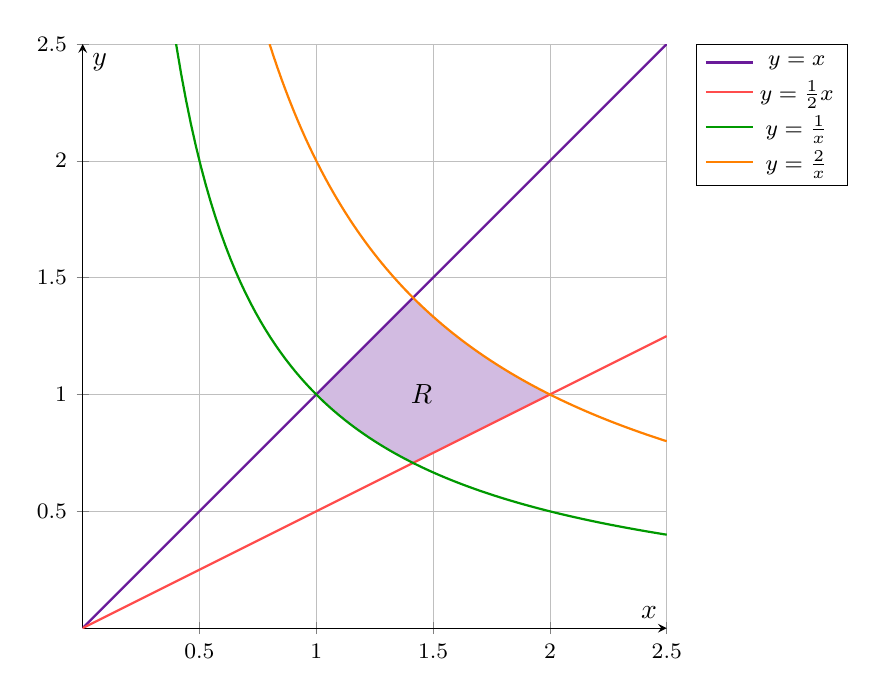
\begin{tikzpicture}
\begin{axis}[
    axis lines=middle,
    xlabel={$x$},
    ylabel={$y$},
    xmin=0, xmax=2.5,
    ymin=0, ymax=2.5,
    samples=100,
    grid=both,
    grid style={line width=.1pt, draw=gray!20},
    major grid style={line width=.2pt,draw=gray!50},
    ticklabel style={font=\footnotesize},
    width=9cm, height=9cm,
    legend style={at={(1.05,1)}, anchor=north west, font=\footnotesize}
]

% Fill the region R
\fill[cD!30] 
    plot[domain=1:1.4142, samples=50] (axis cs:\x, {\x}) --
    plot[domain=1.4142:2, samples=50] (axis cs:\x, {2/\x}) --
    plot[domain=2:1.4142, samples=50] (axis cs:\x, {\x/2}) --
    plot[domain=1.4142:1, samples=50] (axis cs:\x, {1/\x}) -- cycle;

% Draw the boundary curves
\addplot [thick, cD, domain=0:2.5] {x};
\addlegendentry{$y=x$}

\addplot [thick, red!70, domain=0:2.5] {0.5*x};
\addlegendentry{$y=\frac{1}{2}x$}

\addplot [thick, green!60!black, domain=0.4:2.5] {1/x};
\addlegendentry{$y=\frac{1}{x}$}

\addplot [thick, orange, domain=0.8:2.5] {2/x};
\addlegendentry{$y=\frac{2}{x}$}

% Label the Region
\node at (axis cs:1.45, 1) {\textbf{$R$}};

\end{axis}
\end{tikzpicture}
\end{center}

\vspace{1em}
\textbf{2. 3D Surface Representation}

To visualize the volume we are computing, here is the 3D surface $z = e^{xy}$ plotted strictly over the region $R$. 

\begin{center}
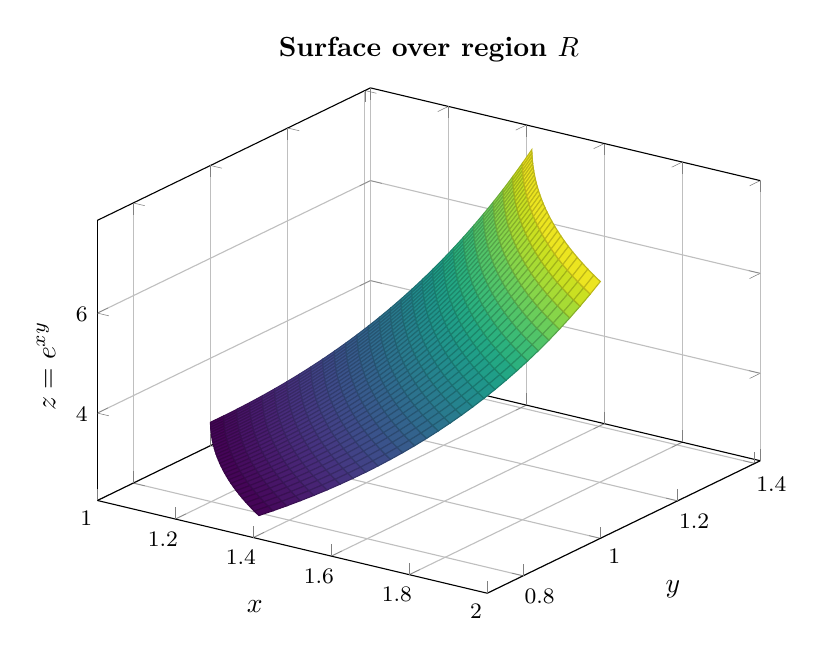
\begin{tikzpicture}
\begin{axis}[
    view={35}{30},
    xlabel={$x$},
    ylabel={$y$},
    zlabel={$z = e^{xy}$},
    title={\textbf{Surface over region $R$}},
    grid=major,
    colormap/viridis,
    width=10cm, height=8cm,
    ticklabel style={font=\footnotesize}
]
% Plotting using the parametric transformation x = sqrt(u/v), y = sqrt(u*v)
\addplot3 [
    surf,
    variable=\u,
    variable y=\v,
    domain=1:2,
    domain y=0.5:1,
    samples=30,
    samples y=30,
    z buffer=sort
] ({sqrt(\u/\v)}, {sqrt(\u*\v)}, {exp(\u)});
\end{axis}
\end{tikzpicture}
\end{center}

\vspace{1em}
\textbf{3. Coordinate Transformation}

To evaluate the integral efficiently, we introduce the transformation of variables:
\[ u = xy \quad \text{and} \quad v = \frac{y}{x} \]

Under this transformation, the boundary curves map to simple constant bounds in the $uv$-plane:
\begin{align*}
    1 \leq &u \leq 2 \\
    \frac{1}{2} \leq &v \leq 1
\end{align*}

\vspace{1em}
\textbf{4. Computing the Jacobian}

We need to compute the Jacobian of the transformation, $J = \frac{\partial(x,y)}{\partial(u,v)}$. It is often easier to compute the inverse Jacobian first:
\[ \frac{\partial(u,v)}{\partial(x,y)} = \begin{vmatrix} 
    \frac{\partial u}{\partial x} & \frac{\partial u}{\partial y} \\[1ex]
    \frac{\partial v}{\partial x} & \frac{\partial v}{\partial y} 
\end{vmatrix} 
= \begin{vmatrix} 
    y & x \\[1ex]
    -\frac{y}{x^2} & \frac{1}{x} 
\end{vmatrix} \]

Evaluating the determinant:
\[ \frac{\partial(u,v)}{\partial(x,y)} = (y)\left(\frac{1}{x}\right) - (x)\left(-\frac{y}{x^2}\right) = \frac{y}{x} + \frac{y}{x} = \frac{2y}{x} = 2v \]

Thus, the required Jacobian is the reciprocal:
\[ |J| = \left| \frac{\partial(x,y)}{\partial(u,v)} \right| = \frac{1}{2v} \]
This gives the area element relationship: $dA = dx\,dy = \frac{1}{2v}\,du\,dv$.

\vspace{1em}
\textbf{5. Evaluating the Integral}

Substitute the new variables, limits, and the area element into the original integral:
\begin{align*}
    \iint_{R} e^{xy} \, dA &= \int_{1/2}^{1} \int_{1}^{2} e^{u} \left( \frac{1}{2v} \right) \, du \, dv \\
    &= \frac{1}{2} \left( \int_{1}^{2} e^{u} \, du \right) \left( \int_{1/2}^{1} \frac{1}{v} \, dv \right)
\end{align*}

Evaluate the two single-variable integrals independently:
\begin{itemize}
    \item Integration with respect to $u$:
    \[ \int_{1}^{2} e^{u} \, du = \left[ e^{u} \right]_{1}^{2} = e^2 - e \]
    
    \item Integration with respect to $v$:
    \[ \int_{1/2}^{1} \frac{1}{v} \, dv = \left[ \ln|v| \right]_{1/2}^{1} = \ln(1) - \ln\left(\frac{1}{2}\right) = 0 - (-\ln 2) = \ln 2 \]
\end{itemize}

Multiplying these results together yields the final answer:
\[ \iint_{R} e^{xy} \, dA = \frac{1}{2} (e^2 - e) \ln 2 \]

\vspace{1em}
\textbf{Final Result:}
\[ \boxed{ \frac{e(e-1)\ln 2}{2} } \]

\end{tcolorbox}

\item Define Jacobian matrix, Hessian matrix and Laplacian operator.
\mk{5} \yr{MATH 241 | L-2/T-1 | 2022--23}

\begin{tcolorbox}[enhanced,breakable,ansbox,colback=cD!4,colframe=cD,boxrule=0.8pt,arc=5pt,title={\textbf{Answer}},fonttitle=\bfseries\color{white},colbacktitle=cD]

\textbf{1. Jacobian Matrix:} \\
Let $\mathbf{f}: \mathbb{R}^n \to \mathbb{R}^m$ be a vector-valued function taking as input the vector $\mathbf{x} = [x_1, x_2, \dots, x_n]^T$ and producing the output vector $\mathbf{f}(\mathbf{x}) = [f_1(\mathbf{x}), f_2(\mathbf{x}), \dots, f_m(\mathbf{x})]^T$. The Jacobian matrix $\mathbf{J}$ is the $m \times n$ matrix containing all first-order partial derivatives of $\mathbf{f}$:
\begin{align*}
\mathbf{J} = \frac{\partial \mathbf{f}}{\partial \mathbf{x}} = 
\begin{bmatrix}
\dfrac{\partial f_1}{\partial x_1} & \dfrac{\partial f_1}{\partial x_2} & \cdots & \dfrac{\partial f_1}{\partial x_n} \\[1ex]
\dfrac{\partial f_2}{\partial x_1} & \dfrac{\partial f_2}{\partial x_2} & \cdots & \dfrac{\partial f_2}{\partial x_n} \\
\vdots & \vdots & \ddots & \vdots \\
\dfrac{\partial f_m}{\partial x_1} & \dfrac{\partial f_m}{\partial x_2} & \cdots & \dfrac{\partial f_m}{\partial x_n}
\end{bmatrix}
\end{align*}

\vspace{1em}
\textbf{2. Hessian Matrix:} \\
Let $f: \mathbb{R}^n \to \mathbb{R}$ be a scalar-valued function. The Hessian matrix $\mathbf{H}$ (or $\nabla^2 f$) is the $n \times n$ square matrix containing all second-order partial derivatives of $f$:
\begin{align*}
\mathbf{H} = 
\begin{bmatrix}
\dfrac{\partial^2 f}{\partial x_1^2} & \dfrac{\partial^2 f}{\partial x_1 \partial x_2} & \cdots & \dfrac{\partial^2 f}{\partial x_1 \partial x_n} \\[1.5ex]
\dfrac{\partial^2 f}{\partial x_2 \partial x_1} & \dfrac{\partial^2 f}{\partial x_2^2} & \cdots & \dfrac{\partial^2 f}{\partial x_2 \partial x_n} \\
\vdots & \vdots & \ddots & \vdots \\
\dfrac{\partial^2 f}{\partial x_n \partial x_1} & \dfrac{\partial^2 f}{\partial x_n \partial x_2} & \cdots & \dfrac{\partial^2 f}{\partial x_n^2}
\end{bmatrix}
\end{align*}
If the second partial derivatives are continuous, the Hessian matrix is symmetric by Schwarz's theorem.

\vspace{1em}
\textbf{3. Laplacian Operator:} \\
The Laplacian operator, denoted by $\nabla^2$ or $\Delta$, is a second-order differential operator defined as the divergence of the gradient ($\nabla \cdot \nabla$) of a scalar-valued function $f: \mathbb{R}^n \to \mathbb{R}$. In Cartesian coordinates, it is the sum of the unmixed second partial derivatives (the trace of the Hessian matrix):
\begin{align*}
\nabla^2 f = \sum_{i=1}^n \frac{\partial^2 f}{\partial x_i^2} = \frac{\partial^2 f}{\partial x_1^2} + \frac{\partial^2 f}{\partial x_2^2} + \cdots + \frac{\partial^2 f}{\partial x_n^2}
\end{align*}

\end{tcolorbox}

\item Evaluate $\displaystyle\iint_{R}\frac{x-y}{x+y}\,dA$ where $R$ is the region enclosed by $x-y=0$, $x-y=1$, $x+y=1$ and $x+y=3$.
\mk{10} \yr{MATH 241 | L-2/T-1 | 2022--23}

\begin{tcolorbox}[enhanced,breakable,ansbox,colback=cD!4,colframe=cD,boxrule=0.8pt,arc=5pt,title={\textbf{Answer}},fonttitle=\bfseries\color{white},colbacktitle=cD]

\textbf{1. Region of Integration}

The region $R$ is bounded by the following lines in the $xy$-plane:
\begin{align*}
    x - y &= 0 \\
    x - y &= 1 \\
    x + y &= 1 \\
    x + y &= 3
\end{align*}

Below is the 2D graph of the region $R$:

\begin{center}
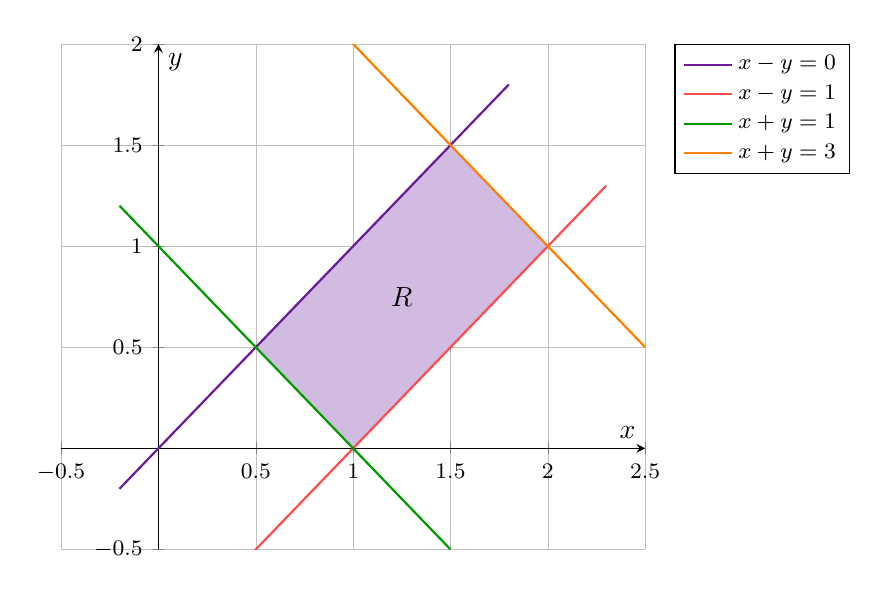
\begin{tikzpicture}
\begin{axis}[
    axis lines=middle,
    xlabel={$x$},
    ylabel={$y$},
    xmin=-0.5, xmax=2.5,
    ymin=-0.5, ymax=2.0,
    samples=100,
    grid=both,
    grid style={line width=.1pt, draw=gray!20},
    major grid style={line width=.2pt,draw=gray!50},
    ticklabel style={font=\footnotesize},
    width=9cm, height=8cm,
    legend style={at={(1.05,1)}, anchor=north west, font=\footnotesize}
]

% Fill the region R by specifying the vertices of the quadrilateral
\fill[cD!30] (axis cs:0.5, 0.5) -- (axis cs:1, 0) -- (axis cs:2, 1) -- (axis cs:1.5, 1.5) -- cycle;

% Draw the boundary lines
\addplot [thick, cD, domain=-0.2:1.8] {x};
\addlegendentry{$x-y=0$}

\addplot [thick, red!70, domain=0.3:2.3] {x-1};
\addlegendentry{$x-y=1$}

\addplot [thick, green!60!black, domain=-0.2:1.5] {1-x};
\addlegendentry{$x+y=1$}

\addplot [thick, orange, domain=0.5:2.5] {3-x};
\addlegendentry{$x+y=3$}

% Label the Region
\node at (axis cs:1.25, 0.75) {\textbf{$R$}};

\end{axis}
\end{tikzpicture}
\end{center}

\vspace{1em}
\textbf{2. 3D Surface Representation}

To visualize the function $z = \frac{x-y}{x+y}$ over the non-rectangular domain $R$, we apply the parametric equations $x = \frac{u+v}{2}$ and $y = \frac{v-u}{2}$ mapping directly from the $uv$-plane bounds:

\begin{center}
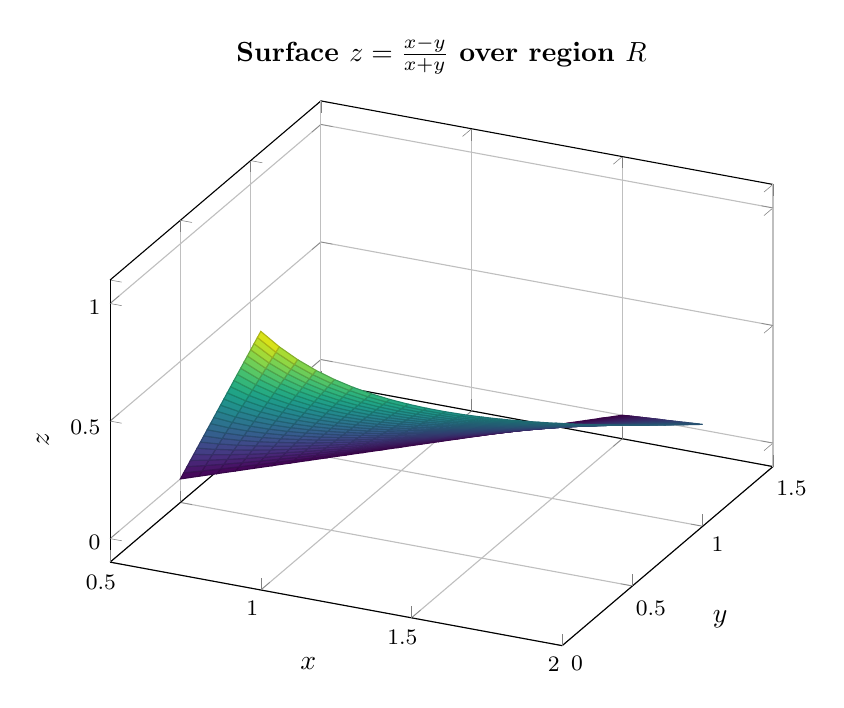
\begin{tikzpicture}
\begin{axis}[
    view={25}{35},
    xlabel={$x$},
    ylabel={$y$},
    zlabel={$z$},
    title={\textbf{Surface $z = \frac{x-y}{x+y}$ over region $R$}},
    grid=major,
    colormap/viridis,
    width=10cm, height=8.5cm,
    ticklabel style={font=\footnotesize}
]
% Plotting using parametric mapping of u and v
\addplot3 [
    surf,
    variable=\u,
    variable y=\v,
    domain=0:1,
    domain y=1:3,
    samples=25,
    samples y=25,
    z buffer=sort
] ({( \u + \v ) / 2}, {( \v - \u ) / 2}, {\u / \v});
\end{axis}
\end{tikzpicture}
\end{center}

\vspace{1em}
\textbf{3. Coordinate Transformation}

To simplify the integrand and the region of integration, we employ a change of variables matching the boundaries:
\[ u = x - y \quad \text{and} \quad v = x + y \]

Under this linear transformation, the boundary lines simplify nicely into constant limits in the $uv$-plane:
\begin{align*}
    0 \leq &u \leq 1 \\
    1 \leq &v \leq 3
\end{align*}

\vspace{1em}
\textbf{4. Computing the Jacobian}

We calculate the Jacobian of the transformation $J = \frac{\partial(x,y)}{\partial(u,v)}$. First, we express $x$ and $y$ explicitly in terms of $u$ and $v$ by adding and subtracting the transformation equations:
\[ x = \frac{u+v}{2} \quad \text{and} \quad y = \frac{v-u}{2} \]

Now, we evaluate the Jacobian determinant:
\[ J = \frac{\partial(x,y)}{\partial(u,v)} = \begin{vmatrix} 
    \frac{\partial x}{\partial u} & \frac{\partial x}{\partial v} \\[1ex]
    \frac{\partial y}{\partial u} & \frac{\partial y}{\partial v} 
\end{vmatrix} 
= \begin{vmatrix} 
    \frac{1}{2} & \frac{1}{2} \\[1ex]
    -\frac{1}{2} & \frac{1}{2} 
\end{vmatrix} \]

\[ J = \left(\frac{1}{2}\right)\left(\frac{1}{2}\right) - \left(\frac{1}{2}\right)\left(-\frac{1}{2}\right) = \frac{1}{4} + \frac{1}{4} = \frac{1}{2} \]

Thus, the area element transforms as: $dA = dx\,dy = |J|\,du\,dv = \frac{1}{2}\,du\,dv$.

\vspace{1em}
\textbf{5. Evaluating the Integral}

Substituting $u$, $v$, the integration boundaries, and the transformed area element into the original integral gives:
\begin{align*}
    \iint_{R} \frac{x-y}{x+y} \, dA &= \int_{1}^{3} \int_{0}^{1} \frac{u}{v} \left( \frac{1}{2} \right) \, du \, dv \\
    &= \frac{1}{2} \left( \int_{0}^{1} u \, du \right) \left( \int_{1}^{3} \frac{1}{v} \, dv \right)
\end{align*}

Now, evaluate the two single-variable integrals independently:
\begin{itemize}
    \item Integration with respect to $u$:
    \[ \int_{0}^{1} u \, du = \left[ \frac{u^2}{2} \right]_{0}^{1} = \frac{1}{2} - 0 = \frac{1}{2} \]
    
    \item Integration with respect to $v$:
    \[ \int_{1}^{3} \frac{1}{v} \, dv = \left[ \ln|v| \right]_{1}^{3} = \ln 3 - \ln 1 = \ln 3 \]
\end{itemize}

Multiplying the components together yields:
\[ \iint_{R} \frac{x-y}{x+y} \, dA = \frac{1}{2} \times \frac{1}{2} \times \ln 3 = \frac{1}{4} \ln 3 \]

\vspace{1em}
\textbf{Final Result:}
\[ \boxed{ \frac{1}{4}\ln 3 } \]

\end{tcolorbox}


\end{enumerate}

%%──────────────────────────────────────────────────────────────────────
\subtopic{cD}{Line Integrals}
\label{sub:s4-lineint}

\begin{enumerate}
    
\item Find the work done in moving a particle in $\mathbf{F}(x,y,z)=(3x^{2}+6y)\mathbf{i}-14yz\mathbf{j}+20xz^{2}\mathbf{k}$ along the straight lines from $(1,0,0)$ to $(1,1,0)$ and then to $(1,1,1)$.
\mk{10} \yr{MATH 241 | L-2/T-1 | 2024--25}

\begin{tcolorbox}[enhanced,breakable,ansbox,colback=cD!4,colframe=cD,boxrule=0.8pt,arc=5pt,title={\textbf{Answer}},fonttitle=\bfseries\color{white},colbacktitle=cD]

The work done $W$ by a force field $\mathbf{F}$ along a curve $C$ is given by the line integral:
\begin{align*}
W = \int_{C} \mathbf{F} \cdot d\mathbf{r} = \int_{C} (F_x \, dx + F_y \, dy + F_z \, dz)
\end{align*}
The given force field is $\mathbf{F}(x,y,z) = (3x^{2}+6y)\mathbf{i} - 14yz\mathbf{j} + 20xz^{2}\mathbf{k}$. The path $C$ consists of two straight line segments, $C_1$ and $C_2$.

\begin{center}
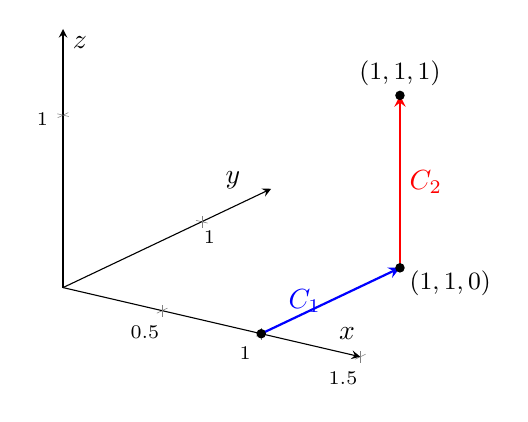
\begin{tikzpicture}
\begin{axis}[
    view={35}{25},
    width=8cm,
    height=7cm,
    xlabel={$x$},
    ylabel={$y$},
    zlabel={$z$},
    xmin=0, xmax=1.5,
    ymin=0, ymax=1.5,
    zmin=0, zmax=1.5,
    grid=major,
    axis lines=center,
    ticklabel style={font=\scriptsize}
]
% Path C1
\addplot3[thick, blue, -stealth] coordinates {(1,0,0) (1,1,0)};
\node[blue, left] at (axis cs:1,0.5,0) {$C_1$};
% Path C2
\addplot3[thick, red, -stealth] coordinates {(1,1,0) (1,1,1)};
\node[red, right] at (axis cs:1,1,0.5) {$C_2$};
% Points
\addplot3[only marks, mark=*, mark size=1.5pt] coordinates {(1,0,0) (1,1,0) (1,1,1)};
\node[below] at (axis cs:1,0,0) {\small $(1,0,0)$};
\node[right, yshift=-2mm] at (axis cs:1,1,0) {\small $(1,1,0)$};
\node[above] at (axis cs:1,1,1) {\small $(1,1,1)$};
\end{axis}
\end{tikzpicture}
\end{center}

\textbf{Step 1: Work done along $C_1$ from $(1,0,0)$ to $(1,1,0)$} \\
Along $C_1$, $x = 1$ and $z = 0$ are constant, while $y$ varies from $0$ to $1$. 
Consequently, $dx = 0$ and $dz = 0$. The differential position vector simplifies to $d\mathbf{r} = dy \, \mathbf{j}$.
The force field along this path simplifies to:
\begin{align*}
F_y = -14yz = -14y(0) = 0
\end{align*}
Thus, the work done along $C_1$ is:
\begin{align*}
W_1 &= \int_{C_1} F_y \, dy = \int_{0}^{1} 0 \, dy = 0
\end{align*}

\textbf{Step 2: Work done along $C_2$ from $(1,1,0)$ to $(1,1,1)$} \\
Along $C_2$, $x = 1$ and $y = 1$ are constant, while $z$ varies from $0$ to $1$. 
Consequently, $dx = 0$ and $dy = 0$. The differential position vector simplifies to $d\mathbf{r} = dz \, \mathbf{k}$.
The force field along this path simplifies to:
\begin{align*}
F_z = 20xz^2 = 20(1)z^2 = 20z^2
\end{align*}
Thus, the work done along $C_2$ is:
\begin{align*}
W_2 &= \int_{C_2} F_z \, dz = \int_{0}^{1} 20z^2 \, dz = 20 \left[ \frac{z^3}{3} \right]_0^1 = \frac{20}{3}
\end{align*}

\textbf{Step 3: Total Work Done} \\
The total work done is the sum of the work done along each segment:
\begin{align*}
W = W_1 + W_2 = 0 + \frac{20}{3} = \frac{20}{3}
\end{align*}

\vspace{1em}
\textbf{Final Answer:}
\begin{align*}
\boxed{ W = \frac{20}{3} }
\end{align*}

\end{tcolorbox}

\item State Green's theorem and verify in the plane for $\displaystyle\oint_{C}(3x^{2}-8y^{2})\,dx+(4y-6xy)\,dy$ where $C$ bounds the region enclosed by $y=\sqrt{x}$ and $y=x^{2}$.
\mk{12} \yr{MATH 241 | L-2/T-1 | 2024--25}

\begin{tcolorbox}[enhanced,breakable,ansbox,colback=cD!4,colframe=cD,boxrule=0.8pt,arc=5pt,title={\textbf{Answer}},fonttitle=\bfseries\color{white},colbacktitle=cD]

\textbf{1. Statement of Green's Theorem} \\
Let $R$ be a simply connected planar region bounded by a piecewise smooth, simple closed curve $C$ oriented counterclockwise. If $L(x,y)$ and $M(x,y)$ are functions with continuous first partial derivatives in an open region containing $R$, then:
\begin{align*}
\oint_C (L \, dx + M \, dy) &= \iint_R \left( \frac{\partial M}{\partial x} - \frac{\partial L}{\partial y} \right) \, dx \, dy
\end{align*}

\textbf{2. Verification} \\
We are given the line integral $\displaystyle\oint_{C}(3x^{2}-8y^{2})\,dx+(4y-6xy)\,dy$ over the boundary $C$ of the region enclosed by $y=\sqrt{x}$ and $y=x^{2}$.
Here, $L(x, y) = 3x^2 - 8y^2$ and $M(x, y) = 4y - 6xy$.

\begin{center}
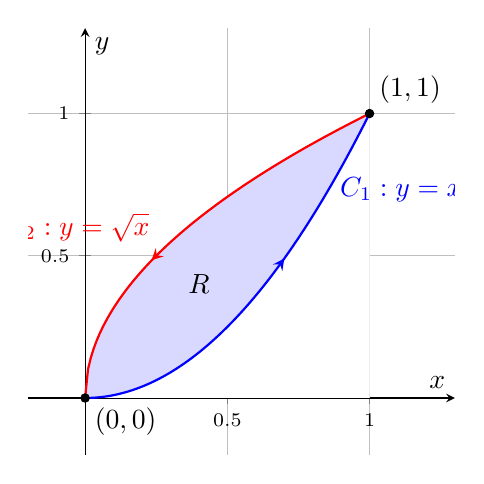
\begin{tikzpicture}
\begin{axis}[
    width=7cm,
    height=7cm,
    xlabel={$x$},
    ylabel={$y$},
    xmin=-0.2, xmax=1.3,
    ymin=-0.2, ymax=1.3,
    axis lines=center,
    grid=both,
    ticklabel style={font=\scriptsize},
    domain=0:1,
    samples=100
]
% Fill region R
\addplot [fill=blue!15, draw=none] {sqrt(x)} \closedcycle;
\addplot [fill=white, draw=none] {x^2} \closedcycle;

% Curve C1: y = x^2
\addplot [thick, blue, postaction={decorate, decoration={markings, mark=at position 0.6 with {\arrow{stealth}}}}] {x^2} node[pos=0.8, right] {$C_1: y=x^2$};

% Curve C2: y = sqrt(x)
\addplot [thick, red, postaction={decorate, decoration={markings, mark=at position 0.4 with {\arrow{stealth reversed}}}}] {sqrt(x)} node[pos=0.4, above left] {$C_2: y=\sqrt{x}$};

% Points of intersection
\addplot[only marks, mark=*, mark size=1.5pt] coordinates {(0,0) (1,1)};
\node[below right] at (axis cs:0,0) {$(0,0)$};
\node[above right] at (axis cs:1,1) {$(1,1)$};
\node at (axis cs:0.4,0.4) {$R$};
\end{axis}
\end{tikzpicture}
\end{center}

\textbf{Step 2.1: Evaluating the Double Integral (Right Hand Side)} \\
First, we find the partial derivatives:
\begin{align*}
\frac{\partial M}{\partial x} &= \frac{\partial}{\partial x}(4y - 6xy) = -6y \\
\frac{\partial L}{\partial y} &= \frac{\partial}{\partial y}(3x^2 - 8y^2) = -16y
\end{align*}
Applying Green's theorem to find the double integral over region $R$:
\begin{align*}
\iint_R \left( \frac{\partial M}{\partial x} - \frac{\partial L}{\partial y} \right) \, dA &= \iint_R (-6y - (-16y)) \, dy \, dx \\
&= \iint_R 10y \, dy \, dx
\end{align*}
The region $R$ is bounded by $x \in [0, 1]$ and $y$ ranges from $x^2$ to $\sqrt{x}$:
\begin{align*}
\text{RHS} &= \int_{0}^{1} \int_{x^2}^{\sqrt{x}} 10y \, dy \, dx \\
&= \int_{0}^{1} \left[ 5y^2 \right]_{x^2}^{\sqrt{x}} dx \\
&= \int_{0}^{1} \left( 5(\sqrt{x})^2 - 5(x^2)^2 \right) dx \\
&= \int_{0}^{1} (5x - 5x^4) \, dx \\
&= \left[ \frac{5x^2}{2} - x^5 \right]_0^1 = \frac{5}{2} - 1 = \frac{3}{2}
\end{align*}

\textbf{Step 2.2: Evaluating the Line Integral (Left Hand Side)} \\
The curve $C$ consists of two parts, $C_1$ (along $y=x^2$) and $C_2$ (along $y=\sqrt{x}$).

\textit{Along $C_1$ (from $x=0$ to $x=1$):} \\
Let $x = t$, $y = t^2$. Then $dx = dt$ and $dy = 2t \, dt$, with $t$ from $0$ to $1$.
\begin{align*}
\int_{C_1} (L \, dx + M \, dy) &= \int_0^1 \left( (3t^2 - 8(t^2)^2) \, dt + (4t^2 - 6t(t^2)) \, (2t \, dt) \right) \\
&= \int_0^1 (3t^2 - 8t^4 + 8t^3 - 12t^4) \, dt \\
&= \int_0^1 (3t^2 + 8t^3 - 20t^4) \, dt \\
&= \left[ t^3 + 2t^4 - 4t^5 \right]_0^1 = 1 + 2 - 4 = -1
\end{align*}

\textit{Along $C_2$ (from $x=1$ to $x=0$):} \\
Let $y = t$, $x = t^2$. Then $dy = dt$ and $dx = 2t \, dt$. Since $x$ goes from $1$ to $0$, $t$ goes from $1$ to $0$.
\begin{align*}
\int_{C_2} (L \, dx + M \, dy) &= \int_1^0 \left( (3(t^2)^2 - 8t^2) \, (2t \, dt) + (4t - 6(t^2)t) \, dt \right) \\
&= \int_1^0 \left( 6t^5 - 16t^3 + 4t - 6t^3 \right) \, dt \\
&= \int_1^0 (6t^5 - 22t^3 + 4t) \, dt \\
&= \left[ t^6 - \frac{11}{2}t^4 + 2t^2 \right]_1^0 \\
&= 0 - \left( 1 - \frac{11}{2} + 2 \right) = - \left( 3 - \frac{11}{2} \right) = \frac{5}{2}
\end{align*}

The total line integral is:
\begin{align*}
\text{LHS} &= \int_{C_1} + \int_{C_2} = -1 + \frac{5}{2} = \frac{3}{2}
\end{align*}

\textbf{Conclusion} \\
Since the LHS (Line Integral) equals the RHS (Double Integral), Green's Theorem is verified.
\begin{align*}
\boxed{\oint_C (L \, dx + M \, dy) = \iint_R \left( \frac{\partial M}{\partial x} - \frac{\partial L}{\partial y} \right) \, dA = \frac{3}{2}}
\end{align*}

\end{tcolorbox}

\item Find the work done by $\mathbf{F}=(3x^{2}+2y)\hat{\mathbf{i}}-(x+3\cos y)\hat{\mathbf{j}}$ around the parallelogram with vertices $(0,0)$, $(2,0)$, $(3,1)$, $(1,1)$.
\mk{13} \yr{MATH 241 | L-2/T-1 | 2023--24}

\begin{tcolorbox}[enhanced,breakable,ansbox,colback=cD!4,colframe=cD,boxrule=0.8pt,arc=5pt,title={\textbf{Answer}},fonttitle=\bfseries\color{white},colbacktitle=cD]

\textbf{1. Formulation of the Problem} \\
The work done by a force field $\mathbf{F} = P\hat{\mathbf{i}} + Q\hat{\mathbf{j}}$ around a closed curve $C$ is given by the line integral:
\begin{align*}
W = \oint_C \mathbf{F} \cdot d\mathbf{r} = \oint_C (P\,dx + Q\,dy)
\end{align*}
Given $\mathbf{F} = (3x^{2}+2y)\hat{\mathbf{i}} - (x+3\cos y)\hat{\mathbf{j}}$, we identify:
\begin{align*}
P(x,y) &= 3x^2 + 2y \\
Q(x,y) &= -(x + 3\cos y) = -x - 3\cos y
\end{align*}
The curve $C$ is the boundary of the parallelogram $R$ with vertices $(0,0)$, $(2,0)$, $(3,1)$, and $(1,1)$, traversed in the counterclockwise direction.

\begin{center}
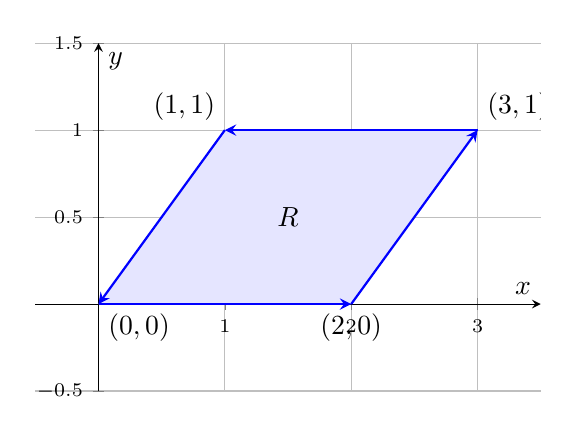
\begin{tikzpicture}
\begin{axis}[
    width=8cm,
    height=6cm,
    xlabel={$x$},
    ylabel={$y$},
    xmin=-0.5, xmax=3.5,
    ymin=-0.5, ymax=1.5,
    axis lines=center,
    grid=both,
    ticklabel style={font=\scriptsize}
]
% Fill region R
\addplot[fill=blue!10, draw=none] coordinates {(0,0) (2,0) (3,1) (1,1) (0,0)};

% Draw boundary with directional arrows
\addplot[thick, blue, -stealth] coordinates {(0,0) (2,0)};
\addplot[thick, blue, -stealth] coordinates {(2,0) (3,1)};
\addplot[thick, blue, -stealth] coordinates {(3,1) (1,1)};
\addplot[thick, blue, -stealth] coordinates {(1,1) (0,0)};

% Labels
\node[below right] at (axis cs:0,0) {$(0,0)$};
\node[below] at (axis cs:2,0) {$(2,0)$};
\node[above right] at (axis cs:3,1) {$(3,1)$};
\node[above left] at (axis cs:1,1) {$(1,1)$};
\node at (axis cs:1.5,0.5) {$R$};
\end{axis}
\end{tikzpicture}
\end{center}

\textbf{2. Applying Green's Theorem} \\
Since $C$ is a simple closed curve bounding the region $R$, we can apply Green's Theorem to convert the line integral into a double integral over $R$:
\begin{align*}
W &= \iint_R \left( \frac{\partial Q}{\partial x} - \frac{\partial P}{\partial y} \right) \, dA
\end{align*}
First, we compute the partial derivatives:
\begin{align*}
\frac{\partial Q}{\partial x} &= \frac{\partial}{\partial x}(-x - 3\cos y) = -1 \\
\frac{\partial P}{\partial y} &= \frac{\partial}{\partial y}(3x^2 + 2y) = 2
\end{align*}
Substitute these into Green's Theorem:
\begin{align*}
W &= \iint_R (-1 - 2) \, dA \\
&= -3 \iint_R \, dA
\end{align*}

\textbf{3. Calculating the Work Done} \\
The double integral $\iint_R \, dA$ represents the area of the region $R$, which is a parallelogram. 
The base of the parallelogram lies along the $x$-axis from $x=0$ to $x=2$, so its length is $b = 2$.
The height of the parallelogram is the perpendicular distance between the lines $y=0$ and $y=1$, so $h = 1$.
\begin{align*}
\text{Area of } R &= \text{base} \times \text{height} = 2 \times 1 = 2
\end{align*}
Thus, substituting the area back into the work equation gives:
\begin{align*}
W &= -3 \times (\text{Area of } R) \\
&= -3 \times 2 = -6
\end{align*}

\vspace{1em}
\textbf{Final Answer:}
\begin{align*}
\boxed{ W = -6 }
\end{align*}

\end{tcolorbox}

\item Find the work done in moving a particle in $\mathbf{F}(x,y,z)=3x^{2}\mathbf{i}+(2xz-y)\mathbf{j}+z\mathbf{k}$ along $x^{2}=4y$, $3x^{3}=8z$ from $x=0$ to $x=2$.
\mk{10/15/22} \yr{MATH 241 | L-2/T-1 | 2022--23} \yr{MATH 147 | L-1/T-2 | 2020--21, 2019--20}


\begin{tcolorbox}[enhanced,breakable,ansbox,colback=cD!4,colframe=cD,boxrule=0.8pt,arc=5pt,title={\textbf{Answer}},fonttitle=\bfseries\color{white},colbacktitle=cD]

\textbf{1. Parameterization of the Curve} \\
The curve $C$ is given by the intersection of the surfaces $x^{2}=4y$ and $3x^{3}=8z$. We can parameterize this curve by setting $x = t$. From the given equations, we find $y$ and $z$ in terms of $t$:
\begin{align*}
x &= t \\
y &= \frac{t^2}{4} \\
z &= \frac{3t^3}{8}
\end{align*}
Since $x$ varies from $0$ to $2$, the parameter $t$ varies from $t = 0$ to $t = 2$.
The position vector of the particle is $\mathbf{r}(t) = t\mathbf{i} + \frac{t^2}{4}\mathbf{j} + \frac{3t^3}{8}\mathbf{k}$.
Taking the differential $d\mathbf{r}$:
\begin{align*}
dx &= dt \\
dy &= \frac{t}{2} \, dt \\
dz &= \frac{9t^2}{8} \, dt
\end{align*}

\begin{center}
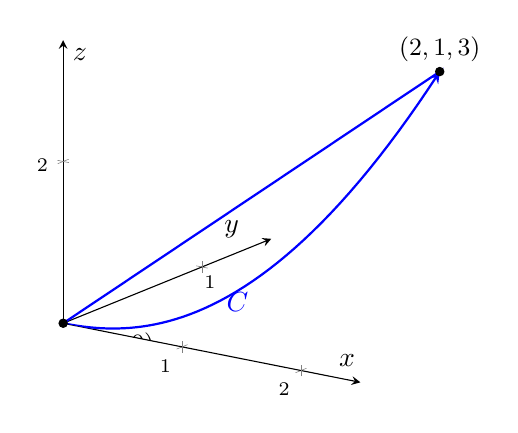
\begin{tikzpicture}
\begin{axis}[
    view={35}{20},
    width=8cm,
    height=7cm,
    xlabel={$x$},
    ylabel={$y$},
    zlabel={$z$},
    xmin=0, xmax=2.5,
    ymin=0, ymax=1.5,
    zmin=0, zmax=3.5,
    grid=major,
    axis lines=center,
    ticklabel style={font=\scriptsize}
]
% Plot parametric curve
\addplot3[
    thick, 
    blue, 
    -stealth, 
    domain=0:2, 
    samples=50
] ({x}, {x^2/4}, {3*x^3/8});

% Nodes and points
\addplot3[only marks, mark=*, mark size=1.5pt] coordinates {(0,0,0) (2,1,3)};
\node[below right] at (axis cs:0,0,0) {\small $(0,0,0)$};
\node[above] at (axis cs:2,1,3) {\small $(2,1,3)$};
\node[blue, right] at (axis cs:1,0.25,0.375) {$C$};
\end{axis}
\end{tikzpicture}
\end{center}

\textbf{2. Formulation of the Work Integral} \\
The work done by the force field $\mathbf{F} = 3x^2\mathbf{i} + (2xz-y)\mathbf{j} + z\mathbf{k}$ is given by the line integral:
\begin{align*}
W &= \int_C \mathbf{F} \cdot d\mathbf{r} = \int_C \left( 3x^2 \, dx + (2xz - y) \, dy + z \, dz \right)
\end{align*}
Substitute the parameterization into the components of $\mathbf{F}$:
\begin{align*}
3x^2 &= 3t^2 \\
2xz - y &= 2(t)\left(\frac{3t^3}{8}\right) - \frac{t^2}{4} = \frac{3t^4}{4} - \frac{t^2}{4} \\
z &= \frac{3t^3}{8}
\end{align*}
Now, substitute the components and differentials into the integral:
\begin{align*}
W &= \int_{0}^{2} \left[ \left(3t^2\right) dt + \left(\frac{3t^4}{4} - \frac{t^2}{4}\right) \left(\frac{t}{2} dt\right) + \left(\frac{3t^3}{8}\right) \left(\frac{9t^2}{8} dt\right) \right] \\
&= \int_{0}^{2} \left( 3t^2 + \frac{3t^5}{8} - \frac{t^3}{8} + \frac{27t^5}{64} \right) dt
\end{align*}

\textbf{3. Simplification and Integration} \\
Combine the like terms (the $t^5$ terms):
\begin{align*}
\frac{3t^5}{8} + \frac{27t^5}{64} &= \frac{24t^5}{64} + \frac{27t^5}{64} = \frac{51t^5}{64}
\end{align*}
The integral becomes:
\begin{align*}
W &= \int_{0}^{2} \left( 3t^2 - \frac{t^3}{8} + \frac{51t^5}{64} \right) dt
\end{align*}
Integrate term by term:
\begin{align*}
W &= \left[ t^3 - \frac{t^4}{32} + \frac{51t^6}{384} \right]_0^2
\end{align*}
Evaluate the definite integral at the upper limit $t = 2$:
\begin{align*}
W &= \left( 2^3 - \frac{2^4}{32} + \frac{51(2^6)}{384} \right) - 0 \\
&= 8 - \frac{16}{32} + \frac{51(64)}{384} \\
&= 8 - \frac{1}{2} + \frac{51}{6} \\
&= 8 - 0.5 + 8.5 \\
&= 16
\end{align*}

\vspace{1em}
\textbf{Final Answer:}
\begin{align*}
\boxed{ W = 16 }
\end{align*}

\end{tcolorbox}

\item State Green's theorem. Verify it for $\displaystyle\oint_{C}(3x^{2}-8y^{2})\,dx+(4y-6xy)\,dy$ where $C$ bounds the region enclosed by $y=x^{2}$ and $x=y^{2}$.
\mk{12} \yr{MATH 241 | L-2/T-1 | 2022--23}

\begin{tcolorbox}[enhanced,breakable,ansbox,colback=cD!4,colframe=cD,boxrule=0.8pt,arc=5pt,title={\textbf{Answer}},fonttitle=\bfseries\color{white},colbacktitle=cD]

\textbf{1. Statement of Green's Theorem} \\
Let $R$ be a simply connected planar region bounded by a piecewise smooth, simple closed curve $C$ oriented counterclockwise. If $L(x,y)$ and $M(x,y)$ are functions with continuous first partial derivatives in an open region containing $R$, then:
\begin{align*}
\oint_C (L \, dx + M \, dy) &= \iint_R \left( \frac{\partial M}{\partial x} - \frac{\partial L}{\partial y} \right) \, dx \, dy
\end{align*}

\textbf{2. Verification} \\
We are given the line integral $\displaystyle\oint_{C}(3x^{2}-8y^{2})\,dx+(4y-6xy)\,dy$ over the boundary $C$ of the region enclosed by $y=x^{2}$ and $x=y^{2}$.
Here, $L(x, y) = 3x^2 - 8y^2$ and $M(x, y) = 4y - 6xy$. 

The curves $y=x^2$ and $x=y^2$ intersect where $x = (x^2)^2 = x^4$, which yields $x=0$ and $x=1$ (since we consider the real plane). The intersection points are $(0,0)$ and $(1,1)$. Note that $x=y^2$ implies $y=\sqrt{x}$ in the first quadrant.

\begin{center}
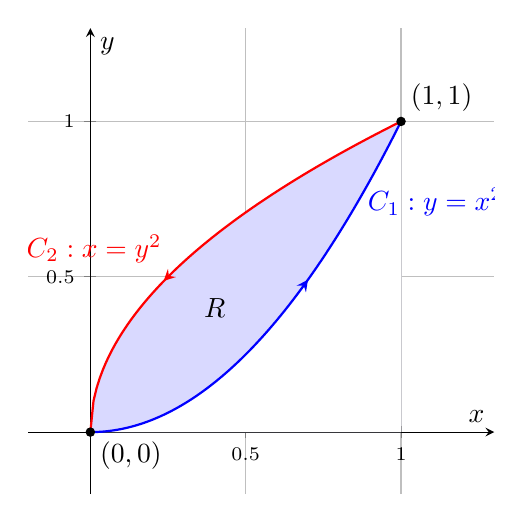
\begin{tikzpicture}
\begin{axis}[
    width=7.5cm,
    height=7.5cm,
    xlabel={$x$},
    ylabel={$y$},
    xmin=-0.2, xmax=1.3,
    ymin=-0.2, ymax=1.3,
    axis lines=center,
    grid=both,
    ticklabel style={font=\scriptsize},
    domain=0:1,
    samples=100
]
% Fill region R
\addplot [fill=blue!15, draw=none] {sqrt(x)} \closedcycle;
\addplot [fill=white, draw=none] {x^2} \closedcycle;

% Curve C1: y = x^2
\addplot [thick, blue, postaction={decorate, decoration={markings, mark=at position 0.6 with {\arrow{stealth}}}}] {x^2} node[pos=0.8, right] {$C_1: y=x^2$};

% Curve C2: x = y^2 -> y = sqrt(x)
\addplot [thick, red, postaction={decorate, decoration={markings, mark=at position 0.4 with {\arrow{stealth reversed}}}}] {sqrt(x)} node[pos=0.4, above left] {$C_2: x=y^2$};

% Points of intersection
\addplot[only marks, mark=*, mark size=1.5pt] coordinates {(0,0) (1,1)};
\node[below right] at (axis cs:0,0) {$(0,0)$};
\node[above right] at (axis cs:1,1) {$(1,1)$};
\node at (axis cs:0.4,0.4) {$R$};
\end{axis}
\end{tikzpicture}
\end{center}

\textbf{Step 2.1: Evaluating the Double Integral (Right Hand Side)} \\
First, we find the partial derivatives of $L$ and $M$:
\begin{align*}
\frac{\partial M}{\partial x} &= \frac{\partial}{\partial x}(4y - 6xy) = -6y \\
\frac{\partial L}{\partial y} &= \frac{\partial}{\partial y}(3x^2 - 8y^2) = -16y
\end{align*}
The integrand for Green's theorem is:
\begin{align*}
\frac{\partial M}{\partial x} - \frac{\partial L}{\partial y} &= -6y - (-16y) = 10y
\end{align*}
The region $R$ is bounded by $x \in [0, 1]$ and $y$ ranges from the lower curve $y = x^2$ to the upper curve $y = \sqrt{x}$:
\begin{align*}
\iint_R \left( \frac{\partial M}{\partial x} - \frac{\partial L}{\partial y} \right) \, dA &= \int_{0}^{1} \int_{x^2}^{\sqrt{x}} 10y \, dy \, dx \\
&= \int_{0}^{1} \left[ 5y^2 \right]_{x^2}^{\sqrt{x}} dx \\
&= \int_{0}^{1} \left( 5(\sqrt{x})^2 - 5(x^2)^2 \right) dx \\
&= \int_{0}^{1} (5x - 5x^4) \, dx \\
&= \left[ \frac{5x^2}{2} - x^5 \right]_0^1 = \frac{5}{2} - 1 = \frac{3}{2}
\end{align*}

\textbf{Step 2.2: Evaluating the Line Integral (Left Hand Side)} \\
The boundary curve $C$ consists of two segments: $C_1$ along $y=x^2$ from $(0,0)$ to $(1,1)$, and $C_2$ along $x=y^2$ from $(1,1)$ back to $(0,0)$.

\textit{Along $C_1$ (from $x=0$ to $x=1$):} \\
Let $x = t$, $y = t^2$. Then $dx = dt$ and $dy = 2t \, dt$.
\begin{align*}
\int_{C_1} (L \, dx + M \, dy) &= \int_0^1 \left( (3t^2 - 8(t^2)^2) \, dt + (4t^2 - 6t(t^2)) \, (2t \, dt) \right) \\
&= \int_0^1 (3t^2 - 8t^4 + 8t^3 - 12t^4) \, dt \\
&= \int_0^1 (3t^2 + 8t^3 - 20t^4) \, dt \\
&= \left[ t^3 + 2t^4 - 4t^5 \right]_0^1 = 1 + 2 - 4 = -1
\end{align*}

\textit{Along $C_2$ (from $y=1$ to $y=0$):} \\
Let $y = t$, $x = t^2$. Then $dy = dt$ and $dx = 2t \, dt$. Since the path goes from $(1,1)$ to $(0,0)$, $t$ varies from $1$ to $0$.
\begin{align*}
\int_{C_2} (L \, dx + M \, dy) &= \int_1^0 \left( (3(t^2)^2 - 8t^2) \, (2t \, dt) + (4t - 6(t^2)t) \, dt \right) \\
&= \int_1^0 \left( 6t^5 - 16t^3 + 4t - 6t^3 \right) \, dt \\
&= \int_1^0 (6t^5 - 22t^3 + 4t) \, dt \\
&= \left[ t^6 - \frac{11}{2}t^4 + 2t^2 \right]_1^0 \\
&= 0 - \left( 1 - \frac{11}{2} + 2 \right) = - \left( 3 - \frac{11}{2} \right) = \frac{5}{2}
\end{align*}

The total line integral over the closed contour $C$ is:
\begin{align*}
\oint_C (L \, dx + M \, dy) &= \int_{C_1} + \int_{C_2} = -1 + \frac{5}{2} = \frac{3}{2}
\end{align*}

\textbf{Conclusion} \\
Both the line integral and the double integral yield the same result. Thus, Green's Theorem is verified.
\begin{align*}
\boxed{\oint_C (L \, dx + M \, dy) = \iint_R \left( \frac{\partial M}{\partial x} - \frac{\partial L}{\partial y} \right) \, dA = \frac{3}{2}}
\end{align*}

\end{tcolorbox}

\item Evaluate $\displaystyle\oint_{C}[(x+2y)\,dx+(x-y)\,dy]$ along $C$: $x=2\cos t$, $y=4\sin t$, $0\le t\le\pi/4$.
\mk{16} \yr{MATH 147 | L-1/T-2 | 2020--21}

\begin{tcolorbox}[enhanced,breakable,ansbox,colback=cD!4,colframe=cD,boxrule=0.8pt,arc=5pt,title={\textbf{Answer}},fonttitle=\bfseries\color{white},colbacktitle=cD]

\textit{Note: Although the closed contour symbol $\oint$ is used in the problem statement, the given limits $0 \le t \le \pi/4$ describe an open arc of an ellipse. We will evaluate the line integral along this specified open path $C$.}

\textbf{1. Parameterization of the Path} \\
The curve $C$ is parametrized by:
\begin{align*}
x &= 2\cos t \implies dx = -2\sin t \, dt \\
y &= 4\sin t \implies dy = 4\cos t \, dt
\end{align*}
for $0 \le t \le \pi/4$. 

\begin{center}
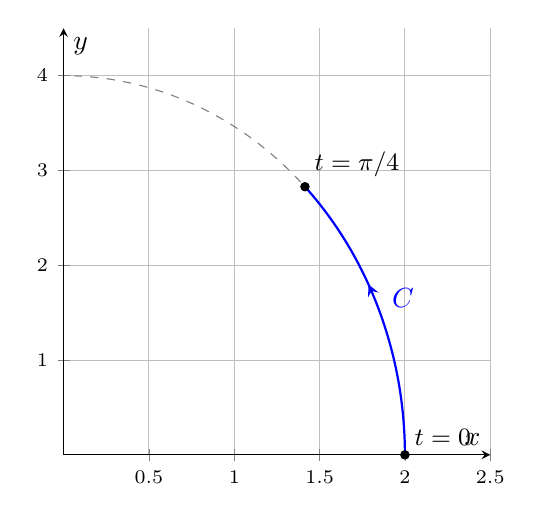
\begin{tikzpicture}
\begin{axis}[
    width=7cm,
    height=7cm,
    xlabel={$x$},
    ylabel={$y$},
    xmin=0, xmax=2.5,
    ymin=0, ymax=4.5,
    axis lines=center,
    grid=major,
    ticklabel style={font=\scriptsize}
]
% Plot the full quarter ellipse lightly
\addplot [dashed, gray, domain=0:pi/2, samples=50] ({2*cos(deg(x))}, {4*sin(deg(x))});

% Plot the specific path C
\addplot [thick, blue, postaction={decorate, decoration={markings, mark=at position 0.6 with {\arrow{stealth}}}}, domain=0:pi/4, samples=50] ({2*cos(deg(x))}, {4*sin(deg(x))}) node[pos=0.5, above right] {$C$};

% Points
\addplot[only marks, mark=*, mark size=1.5pt] coordinates {(2,0) ({2*cos(45)}, {4*sin(45)})};
\node[above right] at (axis cs:2,0) {\small $t=0$};
\node[above right] at (axis cs:{2*cos(45)}, {4*sin(45)}) {\small $t=\pi/4$};
\end{axis}
\end{tikzpicture}
\end{center}

\textbf{2. Substituting into the Integral} \\
We are evaluating the integral:
\begin{align*}
I = \int_{C} [(x+2y)\,dx + (x-y)\,dy]
\end{align*}
Substitute $x$, $y$, $dx$, and $dy$ in terms of $t$:
\begin{align*}
(x+2y) &= 2\cos t + 2(4\sin t) = 2\cos t + 8\sin t \\
(x-y) &= 2\cos t - 4\sin t
\end{align*}
Now, substitute the differentials:
\begin{align*}
(x+2y)\,dx &= (2\cos t + 8\sin t)(-2\sin t \, dt) = -4\sin t \cos t - 16\sin^2 t \, dt \\
(x-y)\,dy &= (2\cos t - 4\sin t)(4\cos t \, dt) = 8\cos^2 t - 16\sin t \cos t \, dt
\end{align*}
Adding these together gives the integrand in terms of $t$:
\begin{align*}
I &= \int_{0}^{\pi/4} \left( -4\sin t \cos t - 16\sin^2 t + 8\cos^2 t - 16\sin t \cos t \right) dt \\
&= \int_{0}^{\pi/4} \left( 8\cos^2 t - 16\sin^2 t - 20\sin t \cos t \right) dt
\end{align*}

\textbf{3. Simplification using Trigonometric Identities} \\
We use the double-angle identities:
$\cos^2 t = \frac{1 + \cos(2t)}{2}$, $\sin^2 t = \frac{1 - \cos(2t)}{2}$, and $2\sin t \cos t = \sin(2t)$.
\begin{align*}
I &= \int_{0}^{\pi/4} \left[ 8\left(\frac{1 + \cos(2t)}{2}\right) - 16\left(\frac{1 - \cos(2t)}{2}\right) - 10\sin(2t) \right] dt \\
&= \int_{0}^{\pi/4} \left[ 4(1 + \cos(2t)) - 8(1 - \cos(2t)) - 10\sin(2t) \right] dt \\
&= \int_{0}^{\pi/4} \left( 4 + 4\cos(2t) - 8 + 8\cos(2t) - 10\sin(2t) \right) dt \\
&= \int_{0}^{\pi/4} \left( -4 + 12\cos(2t) - 10\sin(2t) \right) dt
\end{align*}

\textbf{4. Evaluating the Definite Integral} \\
Integrating term by term:
\begin{align*}
I &= \left[ -4t + 6\sin(2t) + 5\cos(2t) \right]_{0}^{\pi/4}
\end{align*}
Evaluate at the upper limit $t = \pi/4$:
\begin{align*}
\text{Upper} &= -4\left(\frac{\pi}{4}\right) + 6\sin\left(2 \cdot \frac{\pi}{4}\right) + 5\cos\left(2 \cdot \frac{\pi}{4}\right) \\
&= -\pi + 6\sin\left(\frac{\pi}{2}\right) + 5\cos\left(\frac{\pi}{2}\right) \\
&= -\pi + 6(1) + 5(0) = 6 - \pi
\end{align*}
Evaluate at the lower limit $t = 0$:
\begin{align*}
\text{Lower} &= -4(0) + 6\sin(0) + 5\cos(0) \\
&= 0 + 0 + 5(1) = 5
\end{align*}
Subtract the lower limit evaluation from the upper limit evaluation:
\begin{align*}
I &= (6 - \pi) - 5 = 1 - \pi
\end{align*}

\vspace{1em}
\textbf{Final Answer:}
\begin{align*}
\boxed{ I = 1 - \pi }
\end{align*}

\end{tcolorbox}

\item Use Green's Theorem to evaluate $\displaystyle\oint_{C}x^{2}y\,dx-xy^{2}\,dy$ where $C$ bounds the first-quadrant region enclosed by the coordinate axes and the circle $x^{2}+y^{2}=16$.
\mk{$15\tfrac{1}{2}$} \yr{MATH 147 | L-1/T-2 | 2020--21}

\begin{tcolorbox}[enhanced,breakable,ansbox,colback=cD!4,colframe=cD,boxrule=0.8pt,arc=5pt,title={\textbf{Answer}},fonttitle=\bfseries\color{white},colbacktitle=cD]

\textbf{1. Statement of Green's Theorem} \\
Green's Theorem relates a line integral around a simple closed curve $C$ to a double integral over the plane region $R$ bounded by $C$:
\begin{align*}
\oint_C (P \, dx + Q \, dy) &= \iint_R \left( \frac{\partial Q}{\partial x} - \frac{\partial P}{\partial y} \right) \, dA
\end{align*}

\textbf{2. Setting up the Problem} \\
We are given the line integral $\displaystyle\oint_{C} (x^{2}y \, dx - xy^{2} \, dy)$. 
Here, we can identify the functions:
\begin{align*}
P(x,y) &= x^2y \\
Q(x,y) &= -xy^2
\end{align*}
The region $R$ is bounded by the $x$-axis, the $y$-axis, and the circle $x^2 + y^2 = 16$ in the first quadrant.

\begin{center}
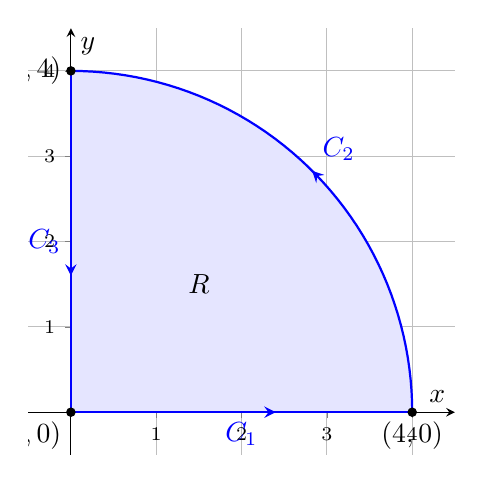
\begin{tikzpicture}
\begin{axis}[
    width=7cm,
    height=7cm,
    xlabel={$x$},
    ylabel={$y$},
    xmin=-0.5, xmax=4.5,
    ymin=-0.5, ymax=4.5,
    axis lines=center,
    grid=both,
    ticklabel style={font=\scriptsize}
]
% Fill region R
\addplot [fill=blue!10, draw=none, domain=0:90, samples=50] ({4*cos(x)}, {4*sin(x)}) \closedcycle;

% Draw boundary C with directional arrows
\addplot [thick, blue, postaction={decorate, decoration={markings, mark=at position 0.6 with {\arrow{stealth}}}}] coordinates {(0,0) (4,0)} node[pos=0.5, below] {$C_1$};
\addplot [thick, blue, postaction={decorate, decoration={markings, mark=at position 0.5 with {\arrow{stealth}}}}, domain=0:90, samples=50] ({4*cos(x)}, {4*sin(x)}) node[pos=0.5, above right] {$C_2$};
\addplot [thick, blue, postaction={decorate, decoration={markings, mark=at position 0.6 with {\arrow{stealth}}}}] coordinates {(0,4) (0,0)} node[pos=0.5, left] {$C_3$};

% Nodes and labels
\addplot[only marks, mark=*, mark size=1.5pt] coordinates {(0,0) (4,0) (0,4)};
\node[below left] at (axis cs:0,0) {$(0,0)$};
\node[below] at (axis cs:4,0) {$(4,0)$};
\node[left] at (axis cs:0,4) {$(0,4)$};
\node at (axis cs:1.5,1.5) {$R$};
\end{axis}
\end{tikzpicture}
\end{center}

\textbf{3. Applying Green's Theorem} \\
First, we compute the necessary partial derivatives:
\begin{align*}
\frac{\partial Q}{\partial x} &= \frac{\partial}{\partial x}(-xy^2) = -y^2 \\
\frac{\partial P}{\partial y} &= \frac{\partial}{\partial y}(x^2y) = x^2
\end{align*}
Substitute these into the right-hand side of Green's Theorem:
\begin{align*}
\iint_R \left( \frac{\partial Q}{\partial x} - \frac{\partial P}{\partial y} \right) \, dA &= \iint_R (-y^2 - x^2) \, dA \\
&= -\iint_R (x^2 + y^2) \, dA
\end{align*}

\textbf{4. Evaluating the Double Integral in Polar Coordinates} \\
Because the region $R$ is a quarter circle, it is most convenient to evaluate the double integral using polar coordinates. 
Let $x = r\cos\theta$ and $y = r\sin\theta$. Then $x^2 + y^2 = r^2$, and $dA = r \, dr \, d\theta$.
For the first-quadrant region enclosed by $x^2 + y^2 = 16$:
\begin{align*}
0 &\le r \le 4 \\
0 &\le \theta \le \frac{\pi}{2}
\end{align*}
Transforming the integral:
\begin{align*}
-\iint_R (x^2 + y^2) \, dA &= -\int_{0}^{\pi/2} \int_{0}^{4} (r^2) \, r \, dr \, d\theta \\
&= -\int_{0}^{\pi/2} d\theta \int_{0}^{4} r^3 \, dr
\end{align*}
Integrate with respect to $\theta$ and $r$ separately:
\begin{align*}
\int_{0}^{\pi/2} d\theta &= [\theta]_0^{\pi/2} = \frac{\pi}{2} \\
\int_{0}^{4} r^3 \, dr &= \left[ \frac{r^4}{4} \right]_0^4 = \frac{4^4}{4} = \frac{256}{4} = 64
\end{align*}
Multiply the results to find the final value:
\begin{align*}
-\left( \frac{\pi}{2} \right) (64) = -32\pi
\end{align*}

\vspace{1em}
\textbf{Final Answer:}
\begin{align*}
\boxed{ \oint_{C} (x^{2}y \, dx - xy^{2} \, dy) = -32\pi }
\end{align*}

\end{tcolorbox}


\item Using Stokes' theorem evaluate $\oint_{C}(\sin z\,dx - \cos x\,dy + \sin y\,dz)$, where $C$ is the boundary of the rectangle $0\le x\le\pi$, $0\le y\le 1$, $z=3$.
\mk{22} \yr{MATH 147 | L-1/T-2 | 2019--20}

\begin{tcolorbox}[enhanced,breakable,ansbox,colback=cD!4,colframe=cD,boxrule=0.8pt,arc=5pt,title={\textbf{Answer}},fonttitle=\bfseries\color{white},colbacktitle=cD]

\textbf{1. Statement of Stokes' Theorem} \\
Stokes' Theorem relates the line integral of a vector field over a simple, closed curve $C$ to a surface integral of the curl of the vector field over any surface $S$ bounded by $C$:
\begin{align*}
\oint_C \mathbf{F} \cdot d\mathbf{r} &= \iint_S (\nabla \times \mathbf{F}) \cdot \hat{\mathbf{n}} \, dS
\end{align*}
where $\hat{\mathbf{n}}$ is the unit normal vector to the surface $S$, and the orientation of $C$ follows the right-hand rule with respect to $\hat{\mathbf{n}}$.

\textbf{2. Identification of the Field and Surface} \\
From the given line integral $\oint_{C} (\sin z \, dx - \cos x \, dy + \sin y \, dz)$, we can identify the vector field $\mathbf{F}$:
\begin{align*}
\mathbf{F} &= P\mathbf{i} + Q\mathbf{j} + R\mathbf{k} \\
&= \sin z \, \mathbf{i} - \cos x \, \mathbf{j} + \sin y \, \mathbf{k}
\end{align*}
The surface $S$ bounded by $C$ is a flat rectangle lying on the plane $z=3$. Its dimensions are given by $0 \le x \le \pi$ and $0 \le y \le 1$. Because the surface lies on a plane parallel to the $xy$-plane, the upward-pointing unit normal vector is:
\begin{align*}
\hat{\mathbf{n}} = \mathbf{k}
\end{align*}
and the differential surface area element is $dS = dx \, dy$.

\begin{center}
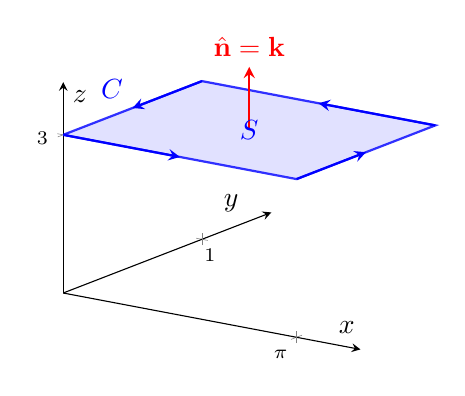
\begin{tikzpicture}
\begin{axis}[
    view={35}{25},
    width=8cm,
    height=6cm,
    xlabel={$x$},
    ylabel={$y$},
    zlabel={$z$},
    xmin=0, xmax=4,
    ymin=0, ymax=1.5,
    zmin=0, zmax=4,
    grid=major,
    axis lines=center,
    ticklabel style={font=\scriptsize},
    xtick={0, 3.14},
    xticklabels={$0$, $\pi$},
    ytick={0, 1},
    ztick={0, 3}
]
% Plot Surface S at z=3
\addplot3[fill=blue!15, draw=blue, thick, opacity=0.8] coordinates {
    (0,0,3) (3.14,0,3) (3.14,1,3) (0,1,3) (0,0,3)
};

% Add normal vector
\draw[-stealth, thick, red] (axis cs:1.57, 0.5, 3) -- (axis cs:1.57, 0.5, 4.2) node[above] {$\hat{\mathbf{n}} = \mathbf{k}$};

% Add path C
\node[blue, above left] at (axis cs:0, 0.5, 3) {$C$};
\node[blue] at (axis cs:1.57, 0.5, 3) {$S$};

% Directional arrows on boundary
\draw[-stealth, thick, blue] (axis cs:0,0,3) -- (axis cs:1.57,0,3);
\draw[-stealth, thick, blue] (axis cs:3.14,0,3) -- (axis cs:3.14,0.5,3);
\draw[-stealth, thick, blue] (axis cs:3.14,1,3) -- (axis cs:1.57,1,3);
\draw[-stealth, thick, blue] (axis cs:0,1,3) -- (axis cs:0,0.5,3);

\end{axis}
\end{tikzpicture}
\end{center}

\textbf{3. Calculation of the Curl} \\
We compute the curl of $\mathbf{F}$, $\nabla \times \mathbf{F}$:
\begin{align*}
\nabla \times \mathbf{F} &= \begin{vmatrix} 
\mathbf{i} & \mathbf{j} & \mathbf{k} \\ 
\frac{\partial}{\partial x} & \frac{\partial}{\partial y} & \frac{\partial}{\partial z} \\ 
\sin z & -\cos x & \sin y 
\end{vmatrix} \\
&= \mathbf{i} \left( \frac{\partial}{\partial y}(\sin y) - \frac{\partial}{\partial z}(-\cos x) \right) - \mathbf{j} \left( \frac{\partial}{\partial x}(\sin y) - \frac{\partial}{\partial z}(\sin z) \right) + \mathbf{k} \left( \frac{\partial}{\partial x}(-\cos x) - \frac{\partial}{\partial y}(\sin z) \right) \\
&= \mathbf{i} (\cos y - 0) - \mathbf{j} (0 - \cos z) + \mathbf{k} (\sin x - 0) \\
&= \cos y \, \mathbf{i} + \cos z \, \mathbf{j} + \sin x \, \mathbf{k}
\end{align*}

\textbf{4. Evaluating the Surface Integral} \\
Next, we find the dot product of the curl and the unit normal vector $\hat{\mathbf{n}} = \mathbf{k}$:
\begin{align*}
(\nabla \times \mathbf{F}) \cdot \hat{\mathbf{n}} &= (\cos y \, \mathbf{i} + \cos z \, \mathbf{j} + \sin x \, \mathbf{k}) \cdot \mathbf{k} \\
&= \sin x
\end{align*}
Now, substitute this into the surface integral over the rectangle $0 \le x \le \pi$ and $0 \le y \le 1$:
\begin{align*}
\iint_S (\nabla \times \mathbf{F}) \cdot \hat{\mathbf{n}} \, dS &= \int_{0}^{1} \int_{0}^{\pi} \sin x \, dx \, dy
\end{align*}
We can evaluate the iterated integral by separating the variables:
\begin{align*}
\int_{0}^{1} dy \cdot \int_{0}^{\pi} \sin x \, dx &= \Big[ y \Big]_0^1 \cdot \Big[ -\cos x \Big]_0^\pi \\
&= (1 - 0) \cdot (-\cos(\pi) - (-\cos(0))) \\
&= 1 \cdot (-(-1) + 1) \\
&= 1 \cdot (1 + 1) \\
&= 2
\end{align*}

\vspace{1em}
\textbf{Final Answer:}
\begin{align*}
\boxed{ \oint_C (\sin z \, dx - \cos x \, dy + \sin y \, dz) = 2 }
\end{align*}

\end{tcolorbox}

\item If $\mathbf{A}=(3x^{2}+6y)\mathbf{i}-14yz\mathbf{j}+20xz^{2}\mathbf{k}$, evaluate $\int_{C}\mathbf{A}\cdot d\mathbf{r}$ from $(0,0,0)$ to $(1,1,1)$ along straight lines $(0,0,0)\to(1,0,0)\to(1,1,0)\to(1,1,1)$.
\mk{16} \yr{MATH 147 | L-1/T-2 | 2017--18}

\begin{tcolorbox}[enhanced,breakable,ansbox,colback=cD!4,colframe=cD,boxrule=0.8pt,arc=5pt,title={\textbf{Answer}},fonttitle=\bfseries\color{white},colbacktitle=cD]

\textbf{1. Setup and Path Division} \\
We are asked to evaluate the line integral 
\begin{align*}
\int_C \mathbf{A} \cdot d\mathbf{r} = \int_C \left( (3x^2+6y)\,dx - 14yz\,dy + 20xz^2\,dz \right)
\end{align*}
The path $C$ consists of three line segments, which we can denote as $C_1$, $C_2$, and $C_3$:
\begin{itemize}
    \item $C_1$: The line segment from $(0,0,0)$ to $(1,0,0)$.
    \item $C_2$: The line segment from $(1,0,0)$ to $(1,1,0)$.
    \item $C_3$: The line segment from $(1,1,0)$ to $(1,1,1)$.
\end{itemize}

\begin{center}
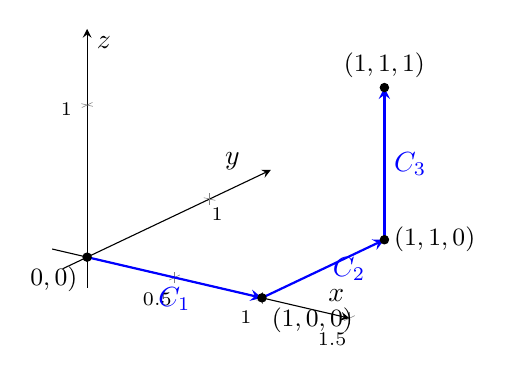
\begin{tikzpicture}
\begin{axis}[
    view={35}{25},
    width=8cm,
    height=7cm,
    xlabel={$x$},
    ylabel={$y$},
    zlabel={$z$},
    xmin=-0.2, xmax=1.5,
    ymin=-0.2, ymax=1.5,
    zmin=-0.2, zmax=1.5,
    grid=major,
    axis lines=center,
    ticklabel style={font=\scriptsize}
]

% Path C1
\addplot3[thick, blue, -stealth] coordinates {(0,0,0) (1,0,0)};
\node[blue, below] at (axis cs:0.5,0,0) {$C_1$};

% Path C2
\addplot3[thick, blue, -stealth] coordinates {(1,0,0) (1,1,0)};
\node[blue, right] at (axis cs:1,0.5,0) {$C_2$};

% Path C3
\addplot3[thick, blue, -stealth] coordinates {(1,1,0) (1,1,1)};
\node[blue, right] at (axis cs:1,1,0.5) {$C_3$};

% Nodes and points
\addplot3[only marks, mark=*, mark size=1.5pt] coordinates {(0,0,0) (1,0,0) (1,1,0) (1,1,1)};
\node[below left] at (axis cs:0,0,0) {\small $(0,0,0)$};
\node[below right] at (axis cs:1,0,0) {\small $(1,0,0)$};
\node[right] at (axis cs:1,1,0) {\small $(1,1,0)$};
\node[above] at (axis cs:1,1,1) {\small $(1,1,1)$};

\end{axis}
\end{tikzpicture}
\end{center}

We evaluate the line integral along each segment individually and sum the results:
\begin{align*}
\int_C \mathbf{A} \cdot d\mathbf{r} = \int_{C_1} \mathbf{A} \cdot d\mathbf{r} + \int_{C_2} \mathbf{A} \cdot d\mathbf{r} + \int_{C_3} \mathbf{A} \cdot d\mathbf{r}
\end{align*}

\textbf{2. Evaluation along $C_1$} \\
Along segment $C_1$ from $(0,0,0)$ to $(1,0,0)$:
\begin{align*}
x &\text{ varies from } 0 \text{ to } 1 \implies dx = dx \\
y &= 0 \implies dy = 0 \\
z &= 0 \implies dz = 0
\end{align*}
Substitute these into the integral:
\begin{align*}
\int_{C_1} \mathbf{A} \cdot d\mathbf{r} &= \int_{0}^{1} \left( (3x^2 + 6(0)) \, dx - 14(0)(0) \, 0 + 20x(0)^2 \, 0 \right) \\
&= \int_{0}^{1} 3x^2 \, dx = \left[ x^3 \right]_0^1 = 1^3 - 0^3 = 1
\end{align*}

\textbf{3. Evaluation along $C_2$} \\
Along segment $C_2$ from $(1,0,0)$ to $(1,1,0)$:
\begin{align*}
x &= 1 \implies dx = 0 \\
y &\text{ varies from } 0 \text{ to } 1 \implies dy = dy \\
z &= 0 \implies dz = 0
\end{align*}
Substitute these into the integral:
\begin{align*}
\int_{C_2} \mathbf{A} \cdot d\mathbf{r} &= \int_{0}^{1} \left( (3(1)^2 + 6y) \, 0 - 14y(0) \, dy + 20(1)(0)^2 \, 0 \right) \\
&= \int_{0}^{1} 0 \, dy = 0
\end{align*}

\textbf{4. Evaluation along $C_3$} \\
Along segment $C_3$ from $(1,1,0)$ to $(1,1,1)$:
\begin{align*}
x &= 1 \implies dx = 0 \\
y &= 1 \implies dy = 0 \\
z &\text{ varies from } 0 \text{ to } 1 \implies dz = dz
\end{align*}
Substitute these into the integral:
\begin{align*}
\int_{C_3} \mathbf{A} \cdot d\mathbf{r} &= \int_{0}^{1} \left( (3(1)^2 + 6(1)) \, 0 - 14(1)z \, 0 + 20(1)z^2 \, dz \right) \\
&= \int_{0}^{1} 20z^2 \, dz = \left[ \frac{20z^3}{3} \right]_0^1 = \frac{20(1)^3}{3} - 0 = \frac{20}{3}
\end{align*}

\textbf{5. Total Work Done} \\
Summing the integrals over the three segments yields the total integral over the path $C$:
\begin{align*}
\int_{C} \mathbf{A} \cdot d\mathbf{r} &= \int_{C_1} \mathbf{A} \cdot d\mathbf{r} + \int_{C_2} \mathbf{A} \cdot d\mathbf{r} + \int_{C_3} \mathbf{A} \cdot d\mathbf{r} \\
&= 1 + 0 + \frac{20}{3} \\
&= \frac{3}{3} + \frac{20}{3} \\
&= \frac{23}{3}
\end{align*}

\vspace{1em}
\textbf{Final Answer:}
\begin{align*}
\boxed{ \int_{C} \mathbf{A} \cdot d\mathbf{r} = \frac{23}{3} }
\end{align*}

\end{tcolorbox}

\item Use a line integral to find the area of the ellipse $x=a\cos t$, $y=b\sin t$, $0\le t\le 2\pi$.
\mk{16} \yr{MATH 147 | L-1/T-2 | 2017--18}

\begin{tcolorbox}[enhanced,breakable,ansbox,colback=cD!4,colframe=cD,boxrule=0.8pt,arc=5pt,title={\textbf{Answer}},fonttitle=\bfseries\color{white},colbacktitle=cD]

\textbf{1. Formula for Area using a Line Integral} \\
By Green's Theorem, the area $A$ of a region enclosed by a simple, closed, counterclockwise curve $C$ can be computed using the line integral:
\begin{align*}
A &= \frac{1}{2} \oint_C (x \, dy - y \, dx)
\end{align*}
(Alternatively, $A = \oint_C x \, dy$ or $A = -\oint_C y \, dx$ can also be used and will yield the same result.)

\textbf{2. Parameterization of the Ellipse} \\
The curve $C$ is an ellipse parameterized by:
\begin{align*}
x &= a\cos t \\
y &= b\sin t
\end{align*}
for $0 \le t \le 2\pi$.

We compute the differentials $dx$ and $dy$ with respect to $t$:
\begin{align*}
dx &= -a\sin t \, dt \\
dy &= b\cos t \, dt
\end{align*}

\begin{center}
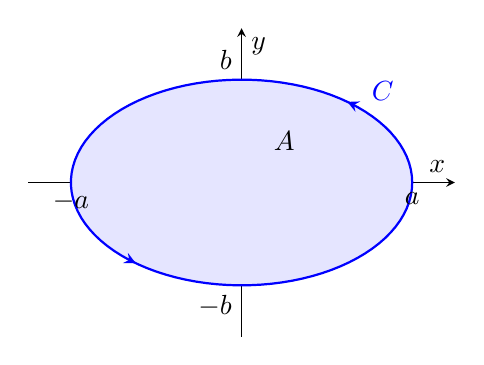
\begin{tikzpicture}
\begin{axis}[
    width=7cm,
    height=5.5cm,
    xlabel={$x$},
    ylabel={$y$},
    xmin=-2.5, xmax=2.5,
    ymin=-1.5, ymax=1.5,
    axis lines=center,
    grid=none,
    ticks=none
]
% Fill region
\addplot [fill=blue!10, draw=none, domain=0:360, samples=100] ({2*cos(x)}, {1*sin(x)}) \closedcycle;

% Draw Ellipse boundary C
\addplot [thick, blue, postaction={decorate, decoration={markings, mark=at position 0.125 with {\arrow{stealth}}, mark=at position 0.625 with {\arrow{stealth}}}}, domain=0:360, samples=100] ({2*cos(x)}, {1*sin(x)});

% Labels
\node[below] at (axis cs:2,0) {$a$};
\node[above left] at (axis cs:0,1) {$b$};
\node[below] at (axis cs:-2,0) {$-a$};
\node[below left] at (axis cs:0,-1) {$-b$};
\node at (axis cs:0.5,0.4) {$A$};
\node[blue, above right] at (axis cs:1.414, 0.707) {$C$};
\end{axis}
\end{tikzpicture}
\end{center}

\textbf{3. Setting up the Integral} \\
Substitute the parametric expressions and their differentials into the area formula:
\begin{align*}
x \, dy &= (a\cos t)(b\cos t \, dt) = ab\cos^2 t \, dt \\
y \, dx &= (b\sin t)(-a\sin t \, dt) = -ab\sin^2 t \, dt
\end{align*}
Now, compute the integrand $x \, dy - y \, dx$:
\begin{align*}
x \, dy - y \, dx &= ab\cos^2 t \, dt - (-ab\sin^2 t \, dt) \\
&= ab(\cos^2 t + \sin^2 t) \, dt \\
&= ab(1) \, dt \\
&= ab \, dt
\end{align*}

\textbf{4. Evaluating the Definite Integral} \\
Now, substitute this back into the formula for $A$ and integrate from $t = 0$ to $t = 2\pi$:
\begin{align*}
A &= \frac{1}{2} \int_{0}^{2\pi} (ab) \, dt \\
&= \frac{ab}{2} \int_{0}^{2\pi} 1 \, dt \\
&= \frac{ab}{2} \Big[ t \Big]_0^{2\pi} \\
&= \frac{ab}{2} (2\pi - 0) \\
&= \pi ab
\end{align*}

\vspace{1em}
\textbf{Final Answer:}
\begin{align*}
\boxed{ A = \pi ab }
\end{align*}

\end{tcolorbox}

\item If $\mathbf{A}=(2y+3)\mathbf{i}+xz\mathbf{j}+(yz-x)\mathbf{k}$, evaluate $\int_{C}\mathbf{A}\cdot d\mathbf{r}$ along straight lines from $(0,0,0)$ to $(1,0,0)$, then to $(1,1,0)$, then to $(2,1,1)$.
\mk{16} \yr{MATH 147 | L-1/T-2 | 2016--17}

\begin{tcolorbox}[enhanced,breakable,ansbox,colback=cD!4,colframe=cD,boxrule=0.8pt,arc=5pt,title={\textbf{Answer}},fonttitle=\bfseries\color{white},colbacktitle=cD]

\textbf{1. Setup and Path Division} \\
We need to evaluate the line integral 
\begin{align*}
\int_C \mathbf{A} \cdot d\mathbf{r} &= \int_C \left( (2y+3)\,dx + xz\,dy + (yz-x)\,dz \right)
\end{align*}
The total path $C$ consists of three distinct straight-line segments, denoted as $C_1$, $C_2$, and $C_3$:
\begin{itemize}
    \item $C_1$: The line segment from $(0,0,0)$ to $(1,0,0)$.
    \item $C_2$: The line segment from $(1,0,0)$ to $(1,1,0)$.
    \item $C_3$: The line segment from $(1,1,0)$ to $(2,1,1)$.
\end{itemize}

\begin{center}
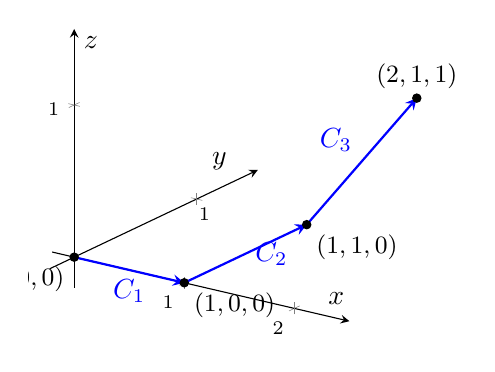
\begin{tikzpicture}
\begin{axis}[
    view={35}{25},
    width=8cm,
    height=7cm,
    xlabel={$x$},
    ylabel={$y$},
    zlabel={$z$},
    xmin=-0.2, xmax=2.5,
    ymin=-0.2, ymax=1.5,
    zmin=-0.2, zmax=1.5,
    grid=major,
    axis lines=center,
    ticklabel style={font=\scriptsize}
]

% Path C1
\addplot3[thick, blue, -stealth] coordinates {(0,0,0) (1,0,0)};
\node[blue, below] at (axis cs:0.5,0,0) {$C_1$};

% Path C2
\addplot3[thick, blue, -stealth] coordinates {(1,0,0) (1,1,0)};
\node[blue, right] at (axis cs:1,0.5,0) {$C_2$};

% Path C3
\addplot3[thick, blue, -stealth] coordinates {(1,1,0) (2,1,1)};
\node[blue, above left] at (axis cs:1.5,1,0.5) {$C_3$};

% Nodes and points
\addplot3[only marks, mark=*, mark size=1.5pt] coordinates {(0,0,0) (1,0,0) (1,1,0) (2,1,1)};
\node[below left] at (axis cs:0,0,0) {\small $(0,0,0)$};
\node[below right] at (axis cs:1,0,0) {\small $(1,0,0)$};
\node[below right] at (axis cs:1,1,0) {\small $(1,1,0)$};
\node[above] at (axis cs:2,1,1) {\small $(2,1,1)$};

\end{axis}
\end{tikzpicture}
\end{center}

We evaluate the line integral along each segment individually and sum the results:
\begin{align*}
\int_C \mathbf{A} \cdot d\mathbf{r} = \int_{C_1} \mathbf{A} \cdot d\mathbf{r} + \int_{C_2} \mathbf{A} \cdot d\mathbf{r} + \int_{C_3} \mathbf{A} \cdot d\mathbf{r}
\end{align*}

\textbf{2. Evaluation along $C_1$} \\
Along segment $C_1$ from $(0,0,0)$ to $(1,0,0)$:
\begin{align*}
x &\text{ varies from } 0 \text{ to } 1 \implies dx = dx \\
y &= 0 \implies dy = 0 \\
z &= 0 \implies dz = 0
\end{align*}
Substitute these into the integral:
\begin{align*}
\int_{C_1} \mathbf{A} \cdot d\mathbf{r} &= \int_{0}^{1} \left( (2(0)+3) \, dx + (x)(0) \, 0 + ((0)(0)-x) \, 0 \right) \\
&= \int_{0}^{1} 3 \, dx = \left[ 3x \right]_0^1 = 3(1) - 0 = 3
\end{align*}

\textbf{3. Evaluation along $C_2$} \\
Along segment $C_2$ from $(1,0,0)$ to $(1,1,0)$:
\begin{align*}
x &= 1 \implies dx = 0 \\
y &\text{ varies from } 0 \text{ to } 1 \implies dy = dy \\
z &= 0 \implies dz = 0
\end{align*}
Substitute these into the integral:
\begin{align*}
\int_{C_2} \mathbf{A} \cdot d\mathbf{r} &= \int_{0}^{1} \left( (2y+3) \, 0 + (1)(0) \, dy + (y(0)-1) \, 0 \right) \\
&= \int_{0}^{1} 0 \, dy = 0
\end{align*}

\textbf{4. Evaluation along $C_3$} \\
Along segment $C_3$ from $(1,1,0)$ to $(2,1,1)$, we can parameterize the line using a parameter $t$ ranging from $0$ to $1$:
\begin{align*}
x &= 1 + t \implies dx = dt \\
y &= 1 \implies dy = 0 \\
z &= t \implies dz = dt
\end{align*}
Substitute these into the integral components:
\begin{align*}
2y + 3 &= 2(1) + 3 = 5 \\
yz - x &= (1)(t) - (1+t) = t - 1 - t = -1
\end{align*}
Now, plug these into the line integral (noting $dy = 0$):
\begin{align*}
\int_{C_3} \mathbf{A} \cdot d\mathbf{r} &= \int_{0}^{1} \left( (5) \, dt + (x)(t) \, 0 + (-1) \, dt \right) \\
&= \int_{0}^{1} (5 - 1) \, dt \\
&= \int_{0}^{1} 4 \, dt = \left[ 4t \right]_0^1 = 4(1) - 0 = 4
\end{align*}

\textbf{5. Total Integral} \\
Summing the integrals over the three segments yields the total integral over the path $C$:
\begin{align*}
\int_{C} \mathbf{A} \cdot d\mathbf{r} &= \int_{C_1} \mathbf{A} \cdot d\mathbf{r} + \int_{C_2} \mathbf{A} \cdot d\mathbf{r} + \int_{C_3} \mathbf{A} \cdot d\mathbf{r} \\
&= 3 + 0 + 4 \\
&= 7
\end{align*}

\vspace{1em}
\textbf{Final Answer:}
\begin{align*}
\boxed{ \int_{C} \mathbf{A} \cdot d\mathbf{r} = 7 }
\end{align*}

\end{tcolorbox}

\item Use a line integral to find the area of the region enclosed by the asteroid $x=a\cos^{3}\phi$, $y=a\sin^{3}\phi$, $0\le\phi\le 2\pi$.
\mk{16} \yr{MATH 147 | L-1/T-2 | 2016--17}

\begin{tcolorbox}[enhanced,breakable,ansbox,colback=cD!4,colframe=cD,boxrule=0.8pt,arc=5pt,title={\textbf{Answer}},fonttitle=\bfseries\color{white},colbacktitle=cD]

\textbf{1. Formula for Area using a Line Integral} \\
By Green's Theorem, the area $A$ of a region enclosed by a simple, closed, counterclockwise curve $C$ can be computed using the line integral:
\begin{align*}
A &= \frac{1}{2} \oint_C (x \, dy - y \, dx)
\end{align*}

\textbf{2. Parameterization of the Astroid} \\
The curve $C$ is an astroid parameterized by:
\begin{align*}
x &= a\cos^3\phi \\
y &= a\sin^3\phi
\end{align*}
for $0 \le \phi \le 2\pi$.

We first compute the differentials $dx$ and $dy$ with respect to $\phi$:
\begin{align*}
dx &= 3a\cos^2\phi(-\sin\phi) \, d\phi = -3a\cos^2\phi\sin\phi \, d\phi \\
dy &= 3a\sin^2\phi(\cos\phi) \, d\phi = 3a\sin^2\phi\cos\phi \, d\phi
\end{align*}

\begin{center}
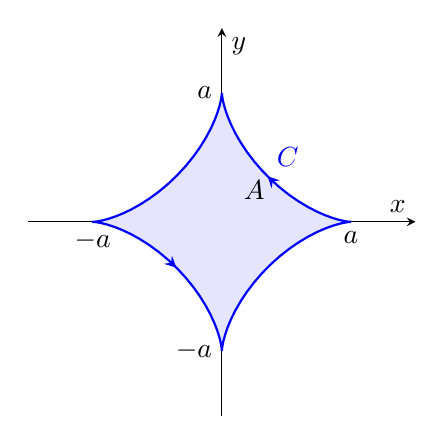
\begin{tikzpicture}
\begin{axis}[
    width=6.5cm,
    height=6.5cm,
    xlabel={$x$},
    ylabel={$y$},
    xmin=-1.5, xmax=1.5,
    ymin=-1.5, ymax=1.5,
    axis lines=center,
    grid=none,
    ticks=none
]
% Fill region
\addplot [fill=blue!10, draw=none, domain=0:360, samples=100] ({cos(x)^3}, {sin(x)^3}) \closedcycle;

% Draw Astroid boundary C
\addplot [thick, blue, postaction={decorate, decoration={markings, mark=at position 0.125 with {\arrow{stealth}}, mark=at position 0.625 with {\arrow{stealth}}}}, domain=0:360, samples=100] ({cos(x)^3}, {sin(x)^3});

% Labels
\node[below] at (axis cs:1,0) {$a$};
\node[left] at (axis cs:0,1) {$a$};
\node[below] at (axis cs:-1,0) {$-a$};
\node[left] at (axis cs:0,-1) {$-a$};
\node at (axis cs:0.25,0.25) {$A$};
\node[blue, above right] at (axis cs:0.35, 0.35) {$C$};
\end{axis}
\end{tikzpicture}
\end{center}

\textbf{3. Setting up the Integral} \\
Substitute the parametric expressions and their differentials into the components of the area formula:
\begin{align*}
x \, dy &= (a\cos^3\phi)(3a\sin^2\phi\cos\phi \, d\phi) = 3a^2\cos^4\phi\sin^2\phi \, d\phi \\
y \, dx &= (a\sin^3\phi)(-3a\cos^2\phi\sin\phi \, d\phi) = -3a^2\sin^4\phi\cos^2\phi \, d\phi
\end{align*}
Now, compute the integrand $x \, dy - y \, dx$:
\begin{align*}
x \, dy - y \, dx &= 3a^2\cos^4\phi\sin^2\phi \, d\phi - (-3a^2\sin^4\phi\cos^2\phi \, d\phi) \\
&= 3a^2\cos^2\phi\sin^2\phi (\cos^2\phi + \sin^2\phi) \, d\phi \\
&= 3a^2\cos^2\phi\sin^2\phi (1) \, d\phi \\
&= 3a^2\cos^2\phi\sin^2\phi \, d\phi
\end{align*}

\textbf{4. Evaluating the Definite Integral} \\
Substitute this simplified expression back into the area formula and integrate from $\phi = 0$ to $\phi = 2\pi$:
\begin{align*}
A &= \frac{1}{2} \int_{0}^{2\pi} 3a^2\cos^2\phi\sin^2\phi \, d\phi \\
&= \frac{3a^2}{2} \int_{0}^{2\pi} (\sin\phi\cos\phi)^2 \, d\phi
\end{align*}
Using the double-angle identity $\sin(2\phi) = 2\sin\phi\cos\phi$, we have $\sin\phi\cos\phi = \frac{1}{2}\sin(2\phi)$:
\begin{align*}
A &= \frac{3a^2}{2} \int_{0}^{2\pi} \left( \frac{\sin(2\phi)}{2} \right)^2 d\phi \\
&= \frac{3a^2}{8} \int_{0}^{2\pi} \sin^2(2\phi) \, d\phi
\end{align*}
Next, use the half-angle identity $\sin^2(2\phi) = \frac{1 - \cos(4\phi)}{2}$:
\begin{align*}
A &= \frac{3a^2}{8} \int_{0}^{2\pi} \frac{1 - \cos(4\phi)}{2} \, d\phi \\
&= \frac{3a^2}{16} \int_{0}^{2\pi} (1 - \cos(4\phi)) \, d\phi \\
&= \frac{3a^2}{16} \left[ \phi - \frac{\sin(4\phi)}{4} \right]_0^{2\pi}
\end{align*}
Evaluate the integral at the boundaries:
\begin{align*}
A &= \frac{3a^2}{16} \left[ \left( 2\pi - \frac{\sin(8\pi)}{4} \right) - \left( 0 - \frac{\sin(0)}{4} \right) \right] \\
&= \frac{3a^2}{16} (2\pi - 0) \\
&= \frac{6\pi a^2}{16} \\
&= \frac{3\pi a^2}{8}
\end{align*}

\vspace{1em}
\textbf{Final Answer:}
\begin{align*}
\boxed{ A = \frac{3\pi a^2}{8} }
\end{align*}

\end{tcolorbox}

\item If $\mathbf{F}=(y^{2}\cos x+z^{3})\mathbf{i}+(2y\sin x-4)\mathbf{j}+(3xz^{2}+2)\mathbf{k}$, show that $\int\mathbf{F}\cdot d\mathbf{r}$ is independent of path. Find the work done in moving an object from $(0,1,-1)$ to $(\pi/2,-1,2)$.
\mk{15} \yr{MATH 147 | L-1/T-2 | 2015--16}

\begin{tcolorbox}[enhanced,breakable,ansbox,colback=cD!4,colframe=cD,boxrule=0.8pt,arc=5pt,title={\textbf{Answer}},fonttitle=\bfseries\color{white},colbacktitle=cD]

\textbf{1. Proving Path Independence} \\
A line integral $\int \mathbf{F} \cdot d\mathbf{r}$ is independent of path in a simply connected domain if the vector field $\mathbf{F}$ is conservative. This is true if the curl of $\mathbf{F}$ is zero, i.e., $\nabla \times \mathbf{F} = \mathbf{0}$.
Let $\mathbf{F} = P\mathbf{i} + Q\mathbf{j} + R\mathbf{k}$, where:
\begin{align*}
P(x,y,z) &= y^{2}\cos x + z^{3} \\
Q(x,y,z) &= 2y\sin x - 4 \\
R(x,y,z) &= 3xz^{2} + 2
\end{align*}
We calculate the curl of $\mathbf{F}$:
\begin{align*}
\nabla \times \mathbf{F} &= \begin{vmatrix} 
\mathbf{i} & \mathbf{j} & \mathbf{k} \\ 
\frac{\partial}{\partial x} & \frac{\partial}{\partial y} & \frac{\partial}{\partial z} \\ 
y^2\cos x + z^3 & 2y\sin x - 4 & 3xz^2 + 2
\end{vmatrix} \\
&= \mathbf{i} \left( \frac{\partial}{\partial y}(3xz^2 + 2) - \frac{\partial}{\partial z}(2y\sin x - 4) \right) \\
&\quad - \mathbf{j} \left( \frac{\partial}{\partial x}(3xz^2 + 2) - \frac{\partial}{\partial z}(y^2\cos x + z^3) \right) \\
&\quad + \mathbf{k} \left( \frac{\partial}{\partial x}(2y\sin x - 4) - \frac{\partial}{\partial y}(y^2\cos x + z^3) \right)
\end{align*}
Evaluating the partial derivatives:
\begin{align*}
\nabla \times \mathbf{F} &= \mathbf{i} (0 - 0) - \mathbf{j} (3z^2 - 3z^2) + \mathbf{k} (2y\cos x - 2y\cos x) \\
&= 0\mathbf{i} + 0\mathbf{j} + 0\mathbf{k} = \mathbf{0}
\end{align*}
Since $\nabla \times \mathbf{F} = \mathbf{0}$ and the component functions have continuous partial derivatives everywhere in $\mathbb{R}^3$, the vector field $\mathbf{F}$ is conservative, and thus the line integral $\int \mathbf{F} \cdot d\mathbf{r}$ is independent of path.

\begin{center}
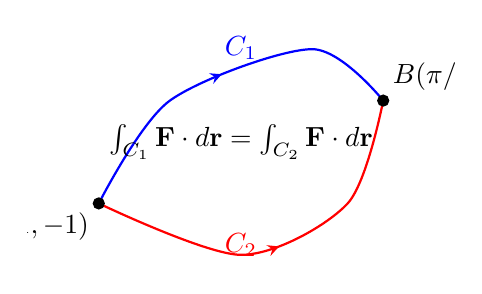
\begin{tikzpicture}
\begin{axis}[
    width=7cm,
    height=5.5cm,
    xmin=-1, xmax=5,
    ymin=-2, ymax=4,
    axis lines=none
]
% Points
\addplot[only marks, mark=*, mark size=2pt] coordinates {(0,0) (4,2)};
\node[below left] at (axis cs:0,0) {$A(0,1,-1)$};
\node[above right] at (axis cs:4,2) {$B(\pi/2,-1,2)$};

% Path 1
\addplot[thick, blue, smooth, postaction={decorate, decoration={markings, mark=at position 0.5 with {\arrow{stealth}}}}] coordinates {(0,0) (1,2) (3,3) (4,2)};
\node[blue, above] at (axis cs:2,2.6) {$C_1$};

% Path 2
\addplot[thick, red, smooth, postaction={decorate, decoration={markings, mark=at position 0.5 with {\arrow{stealth}}}}] coordinates {(0,0) (2,-1) (3.5,0) (4,2)};
\node[red, below] at (axis cs:2,-0.4) {$C_2$};

\node at (axis cs:2, 1.2) {$\int_{C_1} \mathbf{F} \cdot d\mathbf{r} = \int_{C_2} \mathbf{F} \cdot d\mathbf{r}$};

\end{axis}
\end{tikzpicture}
\end{center}

\textbf{2. Finding the Potential Function} \\
Because $\mathbf{F}$ is conservative, there exists a scalar potential function $\phi(x,y,z)$ such that $\nabla\phi = \mathbf{F}$. This gives us three equations:
\begin{align}
\frac{\partial \phi}{\partial x} &= y^2\cos x + z^3 \\
\frac{\partial \phi}{\partial y} &= 2y\sin x - 4 \\
\frac{\partial \phi}{\partial z} &= 3xz^2 + 2
\end{align}
Integrating (1) with respect to $x$:
\begin{align*}
\phi(x,y,z) &= \int (y^2\cos x + z^3) \, dx = y^2\sin x + xz^3 + g(y,z)
\end{align*}
Differentiate this $\phi$ with respect to $y$ and equate to (2):
\begin{align*}
\frac{\partial \phi}{\partial y} &= 2y\sin x + \frac{\partial g}{\partial y} = 2y\sin x - 4 \\
\implies \frac{\partial g}{\partial y} &= -4
\end{align*}
Integrating with respect to $y$, we get $g(y,z) = -4y + h(z)$. Thus,
\begin{align*}
\phi(x,y,z) &= y^2\sin x + xz^3 - 4y + h(z)
\end{align*}
Differentiate this $\phi$ with respect to $z$ and equate to (3):
\begin{align*}
\frac{\partial \phi}{\partial z} &= 3xz^2 + h'(z) = 3xz^2 + 2 \\
\implies h'(z) &= 2
\end{align*}
Integrating with respect to $z$, we get $h(z) = 2z + C$. We can choose $C=0$, giving the potential function:
\begin{align*}
\phi(x,y,z) &= y^2\sin x + xz^3 - 4y + 2z
\end{align*}

\textbf{3. Calculating the Work Done} \\
By the Fundamental Theorem for Line Integrals, the work done moving from point $A(0,1,-1)$ to point $B(\pi/2,-1,2)$ is given by the difference in the potential function evaluated at the endpoints:
\begin{align*}
W &= \int_A^B \mathbf{F} \cdot d\mathbf{r} = \phi(B) - \phi(A)
\end{align*}
Evaluate $\phi$ at the start point $A(0,1,-1)$:
\begin{align*}
\phi(0,1,-1) &= (1)^2\sin(0) + (0)(-1)^3 - 4(1) + 2(-1) \\
&= 0 + 0 - 4 - 2 \\
&= -6
\end{align*}
Evaluate $\phi$ at the end point $B(\pi/2,-1,2)$:
\begin{align*}
\phi(\pi/2,-1,2) &= (-1)^2\sin(\pi/2) + (\pi/2)(2)^3 - 4(-1) + 2(2) \\
&= (1)(1) + (\pi/2)(8) + 4 + 4 \\
&= 1 + 4\pi + 8 \\
&= 9 + 4\pi
\end{align*}
Subtract to find the total work done:
\begin{align*}
W &= (9 + 4\pi) - (-6) \\
&= 15 + 4\pi
\end{align*}

\vspace{1em}
\textbf{Final Answer:}
\begin{align*}
\boxed{ \text{Work Done} = 15 + 4\pi }
\end{align*}

\end{tcolorbox}

\end{enumerate}

%%──────────────────────────────────────────────────────────────────────
\subtopic{cD}{Surface Integrals \& Divergence Theorem}
\label{sub:s4-surface}

\begin{enumerate}
    
    \item Evaluate $\displaystyle\iint_{S}\mathbf{F}\cdot\hat{n}\,dS$ where $\mathbf{F}=(x+y^{2})\mathbf{i}-2x\mathbf{j}+2yz\mathbf{k}$ and $S$ is the surface of the plane $2x+y+2z=6$ in the first octant.
\mk{20} \yr{MATH 147 | L-1/T-2 | 2020--21}

\begin{tcolorbox}[enhanced,breakable,ansbox,colback=cD!4,colframe=cD,boxrule=0.8pt,arc=5pt,title={\textbf{Answer}},fonttitle=\bfseries\color{white},colbacktitle=cD]

\textbf{1. Surface Parameterization and Normal Vector} \\
The surface $S$ is the portion of the plane $2x + y + 2z = 6$ located in the first octant ($x, y, z \ge 0$). We can express $z$ as a function of $x$ and $y$:
\begin{align*}
z &= 3 - x - \frac{1}{2}y
\end{align*}
For a surface defined by $z = g(x,y)$, the upward-pointing differential area vector $\hat{n} \, dS$ is given by:
\begin{align*}
\hat{n} \, dS &= \left( -\frac{\partial z}{\partial x}\mathbf{i} - \frac{\partial z}{\partial y}\mathbf{j} + \mathbf{k} \right) dx \, dy
\end{align*}
Calculating the partial derivatives of $z$:
\begin{align*}
\frac{\partial z}{\partial x} &= -1 \\
\frac{\partial z}{\partial y} &= -\frac{1}{2}
\end{align*}
Substitute these into the normal vector formula:
\begin{align*}
\hat{n} \, dS &= \left( 1\mathbf{i} + \frac{1}{2}\mathbf{j} + 1\mathbf{k} \right) dx \, dy
\end{align*}

\begin{center}
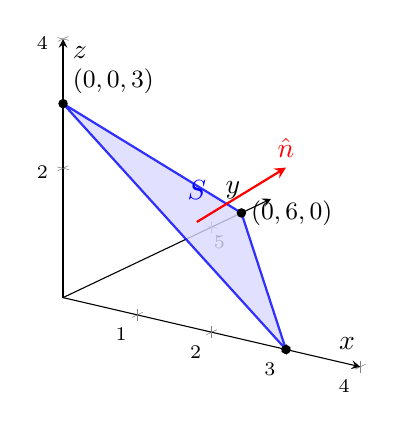
\begin{tikzpicture}
\begin{axis}[
    view={35}{25},
    width=8cm,
    height=7cm,
    xlabel={$x$},
    ylabel={$y$},
    zlabel={$z$},
    xmin=0, xmax=4,
    ymin=0, ymax=7,
    zmin=0, zmax=4,
    grid=major,
    axis lines=center,
    ticklabel style={font=\scriptsize}
]
% Plane S
\addplot3[fill=blue!15, draw=blue, thick, opacity=0.8] coordinates {
    (3,0,0) (0,6,0) (0,0,3) (3,0,0)
};
\node[blue] at (axis cs:1,2,1.5) {$S$};

% Normal vector
\draw[-stealth, thick, red] (axis cs:1,2,1) -- (axis cs:2,2.5,2) node[above] {$\hat{n}$};

% Nodes and points
\addplot3[only marks, mark=*, mark size=1.5pt] coordinates {(3,0,0) (0,6,0) (0,0,3)};
\node[below left] at (axis cs:3,0,0) {\small $(3,0,0)$};
\node[right] at (axis cs:0,6,0) {\small $(0,6,0)$};
\node[above right] at (axis cs:0,0,3) {\small $(0,0,3)$};
\end{axis}
\end{tikzpicture}
\end{center}

\textbf{2. Setting Up the Integrand} \\
We are given the vector field $\mathbf{F} = (x+y^2)\mathbf{i} - 2x\mathbf{j} + 2yz\mathbf{k}$.
Now, we compute the dot product $\mathbf{F} \cdot \hat{n} \, dS$:
\begin{align*}
\mathbf{F} \cdot \hat{n} \, dS &= \left( (x+y^2)\mathbf{i} - 2x\mathbf{j} + 2yz\mathbf{k} \right) \cdot \left( 1\mathbf{i} + \frac{1}{2}\mathbf{j} + 1\mathbf{k} \right) dx \, dy \\
&= \left[ (x+y^2)(1) - 2x\left(\frac{1}{2}\right) + 2yz(1) \right] dx \, dy \\
&= (x + y^2 - x + 2yz) \, dx \, dy \\
&= (y^2 + 2yz) \, dx \, dy
\end{align*}
Next, substitute $z = 3 - x - \frac{1}{2}y$ into the expression so everything is in terms of $x$ and $y$:
\begin{align*}
y^2 + 2yz &= y^2 + 2y\left( 3 - x - \frac{1}{2}y \right) \\
&= y^2 + 6y - 2xy - y^2 \\
&= 6y - 2xy \\
&= y(6 - 2x)
\end{align*}

\textbf{3. Determining the Limits of Integration} \\
The region $R$ in the $xy$-plane is the projection of the surface $S$. Setting $z = 0$ in the plane's equation gives the boundary in the $xy$-plane:
\begin{align*}
2x + y &= 6 \implies y = 6 - 2x
\end{align*}
Since the surface is in the first octant, $x \ge 0$ and $y \ge 0$. The region is bounded by $x=0$, $y=0$, and $y=6-2x$. The limits for $x$ are found by setting $y=0$, which gives $x=3$. Thus, the integration limits are:
\begin{align*}
0 &\le y \le 6 - 2x \\
0 &\le x \le 3
\end{align*}

\textbf{4. Evaluating the Double Integral} \\
Substitute the simplified integrand and limits into the double integral:
\begin{align*}
\iint_S \mathbf{F} \cdot \hat{n} \, dS &= \int_{0}^{3} \int_{0}^{6-2x} y(6 - 2x) \, dy \, dx
\end{align*}
Evaluate the inner integral with respect to $y$:
\begin{align*}
\int_{0}^{6-2x} y(6 - 2x) \, dy &= (6 - 2x) \left[ \frac{y^2}{2} \right]_0^{6-2x} \\
&= \frac{1}{2}(6 - 2x)(6 - 2x)^2 \\
&= \frac{1}{2}(6 - 2x)^3
\end{align*}
Now, substitute this result into the outer integral with respect to $x$:
\begin{align*}
\int_{0}^{3} \frac{1}{2}(6 - 2x)^3 \, dx
\end{align*}
Let $u = 6 - 2x$, then $du = -2 \, dx$, meaning $dx = -\frac{du}{2}$. The new limits are from $u = 6$ (when $x=0$) to $u = 0$ (when $x=3$):
\begin{align*}
\int_{6}^{0} \frac{1}{2}u^3 \left( -\frac{du}{2} \right) &= \frac{1}{4} \int_{0}^{6} u^3 \, du \\
&= \frac{1}{4} \left[ \frac{u^4}{4} \right]_0^6 \\
&= \frac{1}{16} (6^4 - 0) \\
&= \frac{1296}{16} \\
&= 81
\end{align*}

\vspace{1em}
\textbf{Final Answer:}
\begin{align*}
\boxed{ \iint_{S} \mathbf{F} \cdot \hat{n} \, dS = 81 }
\end{align*}

\end{tcolorbox}

\item If $\mathbf{F}=(2x^{2}-3z)\mathbf{i}-2xy\mathbf{j}-4x\mathbf{k}$, evaluate $\displaystyle\iiint_{V}\nabla\cdot\mathbf{F}\,dV$ where $V$ is the closed region bounded by $x=0$, $y=0$, $z=0$ and $2x+2y+z=4$.
\mk{24} \yr{MATH 147 | L-1/T-2 | 2019--20}

\begin{tcolorbox}[enhanced,breakable,ansbox,colback=cD!4,colframe=cD,boxrule=0.8pt,arc=5pt,title={\textbf{Answer}},fonttitle=\bfseries\color{white},colbacktitle=cD]

\textbf{1. Calculation of the Divergence} \\
We are asked to evaluate the volume integral $\iiint_V \nabla \cdot \mathbf{F} \, dV$. First, we must find the divergence of the vector field $\mathbf{F}$, denoted as $\nabla \cdot \mathbf{F}$.
Given $\mathbf{F} = (2x^{2}-3z)\mathbf{i} - 2xy\mathbf{j} - 4x\mathbf{k}$, its components are:
\begin{align*}
F_x &= 2x^2 - 3z \\
F_y &= -2xy \\
F_z &= -4x
\end{align*}
The divergence is defined as the sum of the partial derivatives of each component with respect to its corresponding variable:
\begin{align*}
\nabla \cdot \mathbf{F} &= \frac{\partial F_x}{\partial x} + \frac{\partial F_y}{\partial y} + \frac{\partial F_z}{\partial z} \\
&= \frac{\partial}{\partial x}(2x^2 - 3z) + \frac{\partial}{\partial y}(-2xy) + \frac{\partial}{\partial z}(-4x) \\
&= 4x + (-2x) + 0 \\
&= 2x
\end{align*}

\textbf{2. Defining the Region of Integration} \\
The volume $V$ is bounded by the coordinate planes $x=0$, $y=0$, $z=0$ (which restrict it to the first octant) and the plane $2x + 2y + z = 4$. This forms a tetrahedron.
We can express the limits of integration by finding the intercepts and bounds:
\begin{itemize}
    \item \textbf{For $z$:} Bounded below by $z=0$ and above by the plane $z = 4 - 2x - 2y$.
    \item \textbf{For $y$:} In the $xy$-plane ($z=0$), the boundary line is $2x + 2y = 4$, or $y = 2 - x$. Thus, $y$ ranges from $0$ to $2 - x$.
    \item \textbf{For $x$:} Setting both $y=0$ and $z=0$, we get $2x = 4$, or $x = 2$. Thus, $x$ ranges from $0$ to $2$.
\end{itemize}

\begin{center}
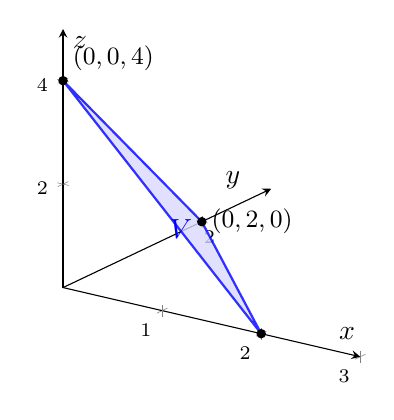
\begin{tikzpicture}
\begin{axis}[
    view={35}{25},
    width=8cm,
    height=7cm,
    xlabel={$x$},
    ylabel={$y$},
    zlabel={$z$},
    xmin=0, xmax=3,
    ymin=0, ymax=3,
    zmin=0, zmax=5,
    grid=major,
    axis lines=center,
    ticklabel style={font=\scriptsize}
]
% Tetrahedron Region V
\addplot3[fill=blue!15, draw=blue, thick, opacity=0.8] coordinates {
    (2,0,0) (0,2,0) (0,0,4) (2,0,0)
};
\node[blue] at (axis cs:0.7,0.7,1) {$V$};

% Nodes and points
\addplot3[only marks, mark=*, mark size=1.5pt] coordinates {(2,0,0) (0,2,0) (0,0,4)};
\node[below left] at (axis cs:2,0,0) {\small $(2,0,0)$};
\node[right] at (axis cs:0,2,0) {\small $(0,2,0)$};
\node[above right] at (axis cs:0,0,4) {\small $(0,0,4)$};
\end{axis}
\end{tikzpicture}
\end{center}

\textbf{3. Evaluating the Volume Integral} \\
We set up the triple integral using the derived divergence and integration limits:
\begin{align*}
I &= \iiint_V (\nabla \cdot \mathbf{F}) \, dV \\
&= \int_{0}^{2} \int_{0}^{2-x} \int_{0}^{4-2x-2y} 2x \, dz \, dy \, dx
\end{align*}

First, integrate with respect to $z$:
\begin{align*}
\int_{0}^{4-2x-2y} 2x \, dz &= \Big[ 2xz \Big]_{0}^{4-2x-2y} \\
&= 2x(4 - 2x - 2y) \\
&= 8x - 4x^2 - 4xy
\end{align*}

Next, substitute this into the middle integral and integrate with respect to $y$:
\begin{align*}
\int_{0}^{2-x} (8x - 4x^2 - 4xy) \, dy &= \left[ (8x - 4x^2)y - 2xy^2 \right]_0^{2-x} \\
&= (8x - 4x^2)(2 - x) - 2x(2 - x)^2
\end{align*}
To simplify, factor out common terms. Note that $8x - 4x^2 = 4x(2 - x)$:
\begin{align*}
(4x(2 - x))(2 - x) - 2x(2 - x)^2 &= 4x(2 - x)^2 - 2x(2 - x)^2 \\
&= 2x(2 - x)^2
\end{align*}
Expand the simplified expression for the final integration:
\begin{align*}
2x(4 - 4x + x^2) &= 8x - 8x^2 + 2x^3
\end{align*}

Finally, substitute this into the outer integral and integrate with respect to $x$:
\begin{align*}
I &= \int_{0}^{2} (8x - 8x^2 + 2x^3) \, dx \\
&= \left[ 4x^2 - \frac{8x^3}{3} + \frac{2x^4}{4} \right]_0^2 \\
&= \left[ 4x^2 - \frac{8}{3}x^3 + \frac{1}{2}x^4 \right]_0^2
\end{align*}
Evaluate the integral at the upper limit $x=2$ (the lower limit evaluates to $0$):
\begin{align*}
I &= 4(2)^2 - \frac{8}{3}(2)^3 + \frac{1}{2}(2)^4 \\
&= 4(4) - \frac{8}{3}(8) + \frac{1}{2}(16) \\
&= 16 - \frac{64}{3} + 8 \\
&= 24 - \frac{64}{3} \\
&= \frac{72 - 64}{3} \\
&= \frac{8}{3}
\end{align*}

\vspace{1em}
\textbf{Final Answer:}
\begin{align*}
\boxed{ \iiint_V \nabla \cdot \mathbf{F} \, dV = \frac{8}{3} }
\end{align*}

\end{tcolorbox}

\item Using the Divergence Theorem evaluate $\displaystyle\iint_{S}\mathbf{F}\cdot\hat{n}\,dS$, where $\mathbf{F}=2xy\mathbf{i}+yz^{2}\mathbf{j}+xz\mathbf{k}$ and $S$ is the surface of the parallelepiped bounded by $x=0$, $y=0$, $z=0$, $x=2$, $y=1$ and $z=3$.
\mk{24} \yr{MATH 147 | L-1/T-2 | 2019--20}

\begin{tcolorbox}[enhanced,breakable,ansbox,colback=cD!4,colframe=cD,boxrule=0.8pt,arc=5pt,title={\textbf{Answer}},fonttitle=\bfseries\color{white},colbacktitle=cD]

\textbf{1. Statement of the Divergence Theorem} \\
The Divergence Theorem (also known as Gauss's Theorem) relates the flux of a vector field through a closed surface $S$ to the volume integral of the divergence of the field over the enclosed region $V$:
\begin{align*}
\iint_S \mathbf{F} \cdot \hat{n} \, dS &= \iiint_V (\nabla \cdot \mathbf{F}) \, dV
\end{align*}

\textbf{2. Calculation of the Divergence} \\
We are given the vector field $\mathbf{F} = 2xy\mathbf{i} + yz^2\mathbf{j} + xz\mathbf{k}$.
First, we find the divergence of $\mathbf{F}$, denoted as $\nabla \cdot \mathbf{F}$:
\begin{align*}
\nabla \cdot \mathbf{F} &= \frac{\partial}{\partial x}(2xy) + \frac{\partial}{\partial y}(yz^2) + \frac{\partial}{\partial z}(xz) \\
&= 2y + z^2 + x
\end{align*}

\textbf{3. Defining the Region of Integration} \\
The region $V$ is a rectangular parallelepiped bounded by the planes $x=0$ to $x=2$, $y=0$ to $y=1$, and $z=0$ to $z=3$. 

\begin{center}
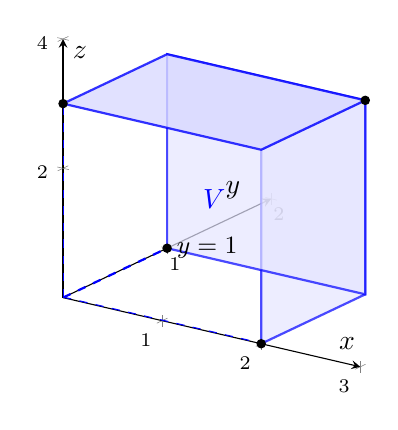
\begin{tikzpicture}
\begin{axis}[
    view={35}{25},
    width=8cm,
    height=7cm,
    xlabel={$x$},
    ylabel={$y$},
    zlabel={$z$},
    xmin=0, xmax=3,
    ymin=0, ymax=2,
    zmin=0, zmax=4,
    grid=major,
    axis lines=center,
    ticklabel style={font=\scriptsize}
]
% Draw back/hidden edges
\draw[dashed, thick, blue] (axis cs:0,0,0) -- (axis cs:2,0,0);
\draw[dashed, thick, blue] (axis cs:0,0,0) -- (axis cs:0,1,0);
\draw[dashed, thick, blue] (axis cs:0,0,0) -- (axis cs:0,0,3);

% Draw visible faces
\addplot3[fill=blue!10, draw=blue, thick, opacity=0.7] coordinates {
    (2,0,0) (2,1,0) (2,1,3) (2,0,3) (2,0,0)
};
\addplot3[fill=blue!10, draw=blue, thick, opacity=0.7] coordinates {
    (0,1,0) (2,1,0) (2,1,3) (0,1,3) (0,1,0)
};
\addplot3[fill=blue!15, draw=blue, thick, opacity=0.8] coordinates {
    (0,0,3) (2,0,3) (2,1,3) (0,1,3) (0,0,3)
};

% Nodes and dimension points
\addplot3[only marks, mark=*, mark size=1.5pt] coordinates {(2,0,0) (0,1,0) (0,0,3) (2,1,3)};
\node[below] at (axis cs:2,0,0) {\small $x=2$};
\node[right] at (axis cs:0,1,0) {\small $y=1$};
\node[left] at (axis cs:0,0,3) {\small $z=3$};
\node[blue] at (axis cs:1,0.5,1.5) {$V$};
\end{axis}
\end{tikzpicture}
\end{center}

\textbf{4. Evaluating the Volume Integral} \\
We can now set up the triple integral using the calculated divergence and the limits of the parallelepiped:
\begin{align*}
\iiint_V (\nabla \cdot \mathbf{F}) \, dV &= \int_{0}^{3} \int_{0}^{1} \int_{0}^{2} (x + 2y + z^2) \, dx \, dy \, dz
\end{align*}

Evaluate the inner integral with respect to $x$:
\begin{align*}
\int_{0}^{2} (x + 2y + z^2) \, dx &= \left[ \frac{x^2}{2} + 2yx + z^2x \right]_0^2 \\
&= \left( \frac{(2)^2}{2} + 2y(2) + z^2(2) \right) - 0 \\
&= 2 + 4y + 2z^2
\end{align*}

Substitute this result into the middle integral and integrate with respect to $y$:
\begin{align*}
\int_{0}^{1} (2 + 4y + 2z^2) \, dy &= \left[ 2y + 2y^2 + 2z^2y \right]_0^1 \\
&= \left( 2(1) + 2(1)^2 + 2z^2(1) \right) - 0 \\
&= 2 + 2 + 2z^2 \\
&= 4 + 2z^2
\end{align*}

Finally, substitute this result into the outer integral and integrate with respect to $z$:
\begin{align*}
\int_{0}^{3} (4 + 2z^2) \, dz &= \left[ 4z + \frac{2z^3}{3} \right]_0^3 \\
&= \left( 4(3) + \frac{2(3)^3}{3} \right) - 0 \\
&= 12 + \frac{2(27)}{3} \\
&= 12 + 18 \\
&= 30
\end{align*}

\vspace{1em}
\textbf{Final Answer:}
\begin{align*}
\boxed{ \iint_S \mathbf{F} \cdot \hat{n} \, dS = 30 }
\end{align*}

\end{tcolorbox}

\item Evaluate $\displaystyle\iiint_{V}\nabla\cdot\mathbf{F}\,dV$ where $\mathbf{F}=yx^{2}\mathbf{i}+(xy^{2}-3z^{4})\mathbf{j}+(x^{3}+y^{3})\mathbf{k}$ and $V$ is the region bounded by $x^{2}+y^{2}+z^{2}=16$, $y\le 0$ and $z\ge 0$.
\mk{25} \yr{MATH 147 | L-1/T-2 | 2018--19}

\begin{tcolorbox}[enhanced,breakable,ansbox,colback=cD!4,colframe=cD,boxrule=0.8pt,arc=5pt,title={\textbf{Answer}},fonttitle=\bfseries\color{white},colbacktitle=cD]

\textbf{1. Calculation of the Divergence} \\
We are tasked to evaluate the volume integral $\iiint_V \nabla \cdot \mathbf{F} \, dV$. First, we compute the divergence of the vector field $\mathbf{F}$, which is defined as:
\begin{align*}
\mathbf{F} &= yx^{2}\mathbf{i} + (xy^{2}-3z^{4})\mathbf{j} + (x^{3}+y^{3})\mathbf{k}
\end{align*}
The divergence is the sum of the partial derivatives of the components with respect to their corresponding variables:
\begin{align*}
\nabla \cdot \mathbf{F} &= \frac{\partial}{\partial x}(yx^2) + \frac{\partial}{\partial y}(xy^2 - 3z^4) + \frac{\partial}{\partial z}(x^3 + y^3) \\
&= 2xy + 2xy + 0 \\
&= 4xy
\end{align*}

\textbf{2. Defining the Region of Integration} \\
The region $V$ is bounded by the sphere $x^2 + y^2 + z^2 = 16$ (which has a radius $R = 4$). We are restricted to $y \le 0$ (the left half of the $xz$-plane) and $z \ge 0$ (the upper half above the $xy$-plane). Thus, $V$ represents a quarter of a solid sphere.

\begin{center}
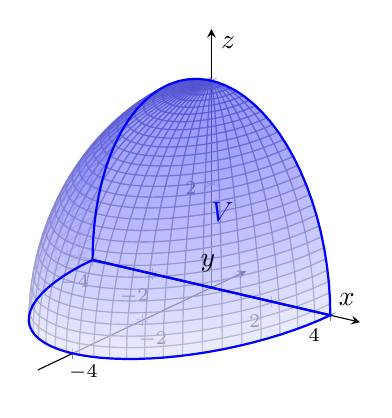
\begin{tikzpicture}
\begin{axis}[
    view={35}{25},
    width=8cm,
    height=7cm,
    xlabel={$x$},
    ylabel={$y$},
    zlabel={$z$},
    xmin=-5, xmax=5,
    ymin=-5, ymax=1,
    zmin=0, zmax=5,
    grid=major,
    axis lines=center,
    ticklabel style={font=\scriptsize}
]
% Plot the spherical surface for y <= 0, z >= 0
\addplot3[
    surf,
    domain=180:360, % theta for y <= 0
    y domain=0:90,  % phi for z >= 0
    samples=30,
    colormap={bluemap}{color=(blue!10) color=(blue!60)},
    opacity=0.7,
    z buffer=sort
]
({4*sin(y)*cos(x)}, {4*sin(y)*sin(x)}, {4*cos(y)});

% Outline of the base
\addplot3[thick, blue, domain=180:360, samples=40] ({4*cos(x)}, {4*sin(x)}, {0});
% Outline of the back plane cross section
\addplot3[thick, blue, domain=0:180, samples=40] ({4*cos(x)}, {0}, {4*sin(x)});

\node[blue, above right] at (axis cs:2,-2,2) {$V$};
\end{axis}
\end{tikzpicture}
\end{center}

We can convert this region into spherical coordinates $(\rho, \theta, \phi)$, where:
\begin{align*}
x &= \rho\sin\phi\cos\theta \\
y &= \rho\sin\phi\sin\theta \\
z &= \rho\cos\phi
\end{align*}
The differential volume element is $dV = \rho^2\sin\phi \, d\rho \, d\phi \, d\theta$.
The limits of integration for the quarter sphere are:
\begin{itemize}
    \item \textbf{Radius:} $0 \le \rho \le 4$
    \item \textbf{Polar angle ($\phi$):} From the positive $z$-axis down to the $xy$-plane ($z \ge 0$), giving $0 \le \phi \le \frac{\pi}{2}$.
    \item \textbf{Azimuthal angle ($\theta$):} In the $xy$-plane where $y \le 0$, which covers the third and fourth quadrants, giving $\pi \le \theta \le 2\pi$.
\end{itemize}

\textbf{3. Evaluating the Volume Integral} \\
We substitute the divergence and spherical coordinate variables into the triple integral:
\begin{align*}
I &= \iiint_V 4xy \, dV \\
&= \int_{\pi}^{2\pi} \int_{0}^{\pi/2} \int_{0}^{4} 4(\rho\sin\phi\cos\theta)(\rho\sin\phi\sin\theta) (\rho^2\sin\phi) \, d\rho \, d\phi \, d\theta
\end{align*}
Simplify the integrand:
\begin{align*}
I &= \int_{\pi}^{2\pi} \int_{0}^{\pi/2} \int_{0}^{4} 4\rho^4 \sin^3\phi \sin\theta \cos\theta \, d\rho \, d\phi \, d\theta
\end{align*}
Since the limits are constants and the integrand is a product of functions of single variables, we can separate the integral into three parts:
\begin{align*}
I &= 4 \left( \int_{0}^{4} \rho^4 \, d\rho \right) \left( \int_{0}^{\pi/2} \sin^3\phi \, d\phi \right) \left( \int_{\pi}^{2\pi} \sin\theta \cos\theta \, d\theta \right)
\end{align*}
We can evaluate the integral with respect to $\theta$ first. Using the substitution $u = \sin\theta \implies du = \cos\theta \, d\theta$, or using the double angle identity $\sin\theta\cos\theta = \frac{1}{2}\sin(2\theta)$:
\begin{align*}
\int_{\pi}^{2\pi} \sin\theta \cos\theta \, d\theta &= \left[ \frac{1}{2}\sin^2\theta \right]_{\pi}^{2\pi} \\
&= \frac{1}{2} (\sin^2(2\pi) - \sin^2(\pi)) \\
&= \frac{1}{2} (0 - 0) \\
&= 0
\end{align*}
Because this multiplier evaluates to $0$, the entire product is zero. 

\textit{Note:} This result could also be deduced using a symmetry argument. The region $V$ is symmetric across the $yz$-plane (it spans from $x=-4$ to $x=4$ evenly), but the integrand $4xy$ is an odd function with respect to $x$ (since replacing $x$ with $-x$ changes the sign to $-4xy$). Therefore, integrating an odd function over a symmetric domain results in exactly zero.

\vspace{1em}
\textbf{Final Answer:}
\begin{align*}
\boxed{ \iiint_{V}\nabla\cdot\mathbf{F}\,dV = 0 }
\end{align*}

\end{tcolorbox}

\item Evaluate $\displaystyle\iint_{S}\mathbf{A}\cdot\hat{n}\,dS$, where $\mathbf{A}=18z\mathbf{i}-12\mathbf{j}+3y\mathbf{k}$ and $S$ is that part of the plane $2x+3y+6z=12$ in the first octant.
\mk{23} \yr{MATH 147 | L-1/T-2 | 2017--18, 2016--17}

\begin{tcolorbox}[enhanced,breakable,ansbox,colback=cD!4,colframe=cD,boxrule=0.8pt,arc=5pt,title={\textbf{Answer}},fonttitle=\bfseries\color{white},colbacktitle=cD]

\textbf{1. Surface Parameterization and Normal Vector} \\
The surface $S$ is the portion of the plane $2x + 3y + 6z = 12$ located in the first octant ($x, y, z \ge 0$). We can express $z$ as a function of $x$ and $y$ by isolating $z$:
\begin{align*}
6z &= 12 - 2x - 3y \\
z &= 2 - \frac{1}{3}x - \frac{1}{2}y
\end{align*}
For a surface defined by $z = g(x,y)$, the upward-pointing differential area vector $\hat{n} \, dS$ is given by:
\begin{align*}
\hat{n} \, dS &= \left( -\frac{\partial z}{\partial x}\mathbf{i} - \frac{\partial z}{\partial y}\mathbf{j} + \mathbf{k} \right) dx \, dy
\end{align*}
Calculating the partial derivatives:
\begin{align*}
\frac{\partial z}{\partial x} &= -\frac{1}{3} \\
\frac{\partial z}{\partial y} &= -\frac{1}{2}
\end{align*}
Substitute these into the normal vector formula:
\begin{align*}
\hat{n} \, dS &= \left( \frac{1}{3}\mathbf{i} + \frac{1}{2}\mathbf{j} + \mathbf{k} \right) dx \, dy
\end{align*}

\begin{center}
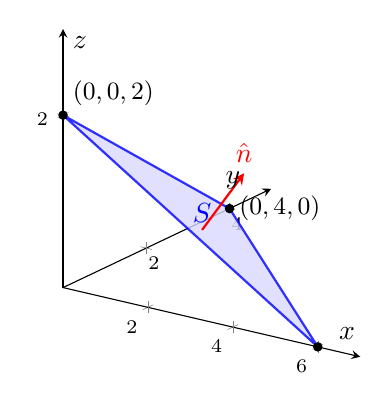
\begin{tikzpicture}
\begin{axis}[
    view={35}{25},
    width=8cm,
    height=7cm,
    xlabel={$x$},
    ylabel={$y$},
    zlabel={$z$},
    xmin=0, xmax=7,
    ymin=0, ymax=5,
    zmin=0, zmax=3,
    grid=major,
    axis lines=center,
    ticklabel style={font=\scriptsize}
]
% Plane S
\addplot3[fill=blue!15, draw=blue, thick, opacity=0.8] coordinates {
    (6,0,0) (0,4,0) (0,0,2) (6,0,0)
};
\node[blue] at (axis cs:2,1.3,0.8) {$S$};

% Normal vector
\draw[-stealth, thick, red] (axis cs:2,1.3,0.6) -- (axis cs:2.5,1.8,1.2) node[above] {$\hat{n}$};

% Nodes and points
\addplot3[only marks, mark=*, mark size=1.5pt] coordinates {(6,0,0) (0,4,0) (0,0,2)};
\node[below left] at (axis cs:6,0,0) {\small $(6,0,0)$};
\node[right] at (axis cs:0,4,0) {\small $(0,4,0)$};
\node[above right] at (axis cs:0,0,2) {\small $(0,0,2)$};
\end{axis}
\end{tikzpicture}
\end{center}

\textbf{2. Setting Up the Integrand} \\
We are given the vector field $\mathbf{A} = 18z\mathbf{i} - 12\mathbf{j} + 3y\mathbf{k}$.
Compute the dot product $\mathbf{A} \cdot \hat{n} \, dS$:
\begin{align*}
\mathbf{A} \cdot \hat{n} \, dS &= \left( 18z\mathbf{i} - 12\mathbf{j} + 3y\mathbf{k} \right) \cdot \left( \frac{1}{3}\mathbf{i} + \frac{1}{2}\mathbf{j} + \mathbf{k} \right) dx \, dy \\
&= \left[ 18z\left(\frac{1}{3}\right) - 12\left(\frac{1}{2}\right) + 3y(1) \right] dx \, dy \\
&= (6z - 6 + 3y) \, dx \, dy
\end{align*}
Now, substitute the plane equation $6z = 12 - 2x - 3y$ into the integrand to express it entirely in terms of $x$ and $y$:
\begin{align*}
6z - 6 + 3y &= (12 - 2x - 3y) - 6 + 3y \\
&= 6 - 2x
\end{align*}
Thus, the differential flux becomes:
\begin{align*}
\mathbf{A} \cdot \hat{n} \, dS &= (6 - 2x) \, dx \, dy
\end{align*}

\textbf{3. Determining the Limits of Integration} \\
The region $R$ in the $xy$-plane is the projection of the surface $S$. Setting $z = 0$ in the plane's equation gives the boundary line in the $xy$-plane:
\begin{align*}
2x + 3y &= 12 \implies 3y = 12 - 2x \implies y = 4 - \frac{2}{3}x
\end{align*}
Since the surface is in the first octant, $x \ge 0$ and $y \ge 0$. The intercepts are found by setting the other variable to zero: the $y$-intercept is $4$ and the $x$-intercept is $6$. Therefore, the limits of integration are:
\begin{align*}
0 &\le y \le 4 - \frac{2}{3}x \\
0 &\le x \le 6
\end{align*}

\textbf{4. Evaluating the Double Integral} \\
Substitute the simplified integrand and the limits into the double integral:
\begin{align*}
\iint_S \mathbf{A} \cdot \hat{n} \, dS &= \int_{0}^{6} \int_{0}^{4 - \frac{2}{3}x} (6 - 2x) \, dy \, dx
\end{align*}
Evaluate the inner integral with respect to $y$. Since the integrand depends only on $x$, it is treated as a constant:
\begin{align*}
\int_{0}^{4 - \frac{2}{3}x} (6 - 2x) \, dy &= (6 - 2x) \Big[ y \Big]_0^{4 - \frac{2}{3}x} \\
&= (6 - 2x) \left( 4 - \frac{2}{3}x \right)
\end{align*}
Expand the product before integrating with respect to $x$:
\begin{align*}
(6 - 2x) \left( 4 - \frac{2}{3}x \right) &= 24 - 4x - 8x + \frac{4}{3}x^2 \\
&= 24 - 12x + \frac{4}{3}x^2
\end{align*}
Now, substitute this polynomial into the outer integral and evaluate with respect to $x$:
\begin{align*}
\int_{0}^{6} \left( 24 - 12x + \frac{4}{3}x^2 \right) dx &= \left[ 24x - 6x^2 + \frac{4}{9}x^3 \right]_0^6
\end{align*}
Evaluate at the upper limit $x = 6$ (the lower limit evaluates to $0$):
\begin{align*}
\left[ 24(6) - 6(6)^2 + \frac{4}{9}(6)^3 \right] &= 144 - 6(36) + \frac{4}{9}(216) \\
&= 144 - 216 + 4(24) \\
&= 144 - 216 + 96 \\
&= 240 - 216 \\
&= 24
\end{align*}

\vspace{1em}
\textbf{Final Answer:}
\begin{align*}
\boxed{ \iint_{S} \mathbf{A} \cdot \hat{n} \, dS = 24 }
\end{align*}

\end{tcolorbox}

\item Use the Divergence Theorem to find the outward flux of $\mathbf{F}=x^{3}\mathbf{i}+y^{3}\mathbf{j}+z^{3}\mathbf{k}$ across the surface of the region enclosed by $z=\sqrt{a^{2}-x^{2}-y^{2}}$ and the plane $z=0$.
\mk{23} \yr{MATH 147 | L-1/T-2 | 2017--18, 2016--17}

\begin{tcolorbox}[enhanced,breakable,ansbox,colback=cD!4,colframe=cD,boxrule=0.8pt,arc=5pt,title={\textbf{Answer}},fonttitle=\bfseries\color{white},colbacktitle=cD]

\textbf{1. Statement of the Divergence Theorem} \\
The Divergence Theorem states that the outward flux of a vector field $\mathbf{F}$ across a closed surface $S$ is equal to the volume integral of the divergence of $\mathbf{F}$ over the region $V$ enclosed by $S$:
\begin{align*}
\iint_S \mathbf{F} \cdot \hat{n} \, dS &= \iiint_V (\nabla \cdot \mathbf{F}) \, dV
\end{align*}

\textbf{2. Calculation of the Divergence} \\
The given vector field is $\mathbf{F} = x^{3}\mathbf{i} + y^{3}\mathbf{j} + z^{3}\mathbf{k}$.
We compute its divergence ($\nabla \cdot \mathbf{F}$):
\begin{align*}
\nabla \cdot \mathbf{F} &= \frac{\partial}{\partial x}(x^3) + \frac{\partial}{\partial y}(y^3) + \frac{\partial}{\partial z}(z^3) \\
&= 3x^2 + 3y^2 + 3z^2 \\
&= 3(x^2 + y^2 + z^2)
\end{align*}

\textbf{3. Defining the Region of Integration} \\
The region $V$ is bounded above by the hemisphere $z = \sqrt{a^{2}-x^{2}-y^{2}}$ and below by the plane $z = 0$. This represents a solid upper hemisphere of radius $a$.

\begin{center}
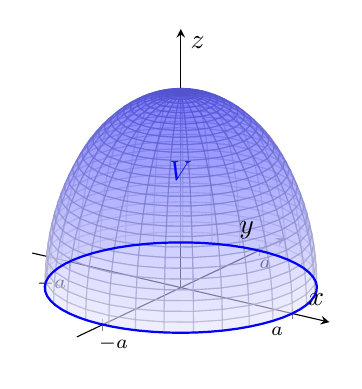
\begin{tikzpicture}
\begin{axis}[
    view={35}{25},
    width=8cm,
    height=7cm,
    xlabel={$x$},
    ylabel={$y$},
    zlabel={$z$},
    xmin=-4, xmax=4,
    ymin=-4, ymax=4,
    zmin=0, zmax=4,
    grid=major,
    axis lines=center,
    ticklabel style={font=\scriptsize},
    xtick={-3,3}, xticklabels={$-a$,$a$},
    ytick={-3,3}, yticklabels={$-a$,$a$},
    ztick={3}, zticklabels={$a$}
]
% Hemispherical surface
\addplot3[
    surf,
    domain=0:360,
    y domain=0:90,
    samples=30,
    colormap={bluemap}{color=(blue!10) color=(blue!60)},
    opacity=0.6,
    z buffer=sort
]
({3*sin(y)*cos(x)}, {3*sin(y)*sin(x)}, {3*cos(y)});

% Base outline (circle at z=0)
\addplot3[thick, blue, domain=0:360, samples=60] ({3*cos(x)}, {3*sin(x)}, {0});

\node[blue, above] at (axis cs:0,0,1.5) {$V$};
\end{axis}
\end{tikzpicture}
\end{center}

Given the spherical symmetry of the region, we switch to spherical coordinates $(\rho, \theta, \phi)$:
\begin{align*}
x^2 + y^2 + z^2 &= \rho^2
\end{align*}
Thus, the divergence simplifies beautifully to:
\begin{align*}
\nabla \cdot \mathbf{F} &= 3\rho^2
\end{align*}
The differential volume element in spherical coordinates is $dV = \rho^2 \sin\phi \, d\rho \, d\phi \, d\theta$.
The limits of integration for the upper hemisphere of radius $a$ are:
\begin{itemize}
    \item \textbf{Radius ($\rho$):} $0 \le \rho \le a$
    \item \textbf{Polar angle ($\phi$):} From the positive $z$-axis down to the $xy$-plane, so $0 \le \phi \le \frac{\pi}{2}$.
    \item \textbf{Azimuthal angle ($\theta$):} A complete circle in the $xy$-plane, so $0 \le \theta \le 2\pi$.
\end{itemize}

\textbf{4. Evaluating the Volume Integral} \\
We can now set up and evaluate the triple integral:
\begin{align*}
\iiint_V (\nabla \cdot \mathbf{F}) \, dV &= \int_{0}^{2\pi} \int_{0}^{\pi/2} \int_{0}^{a} (3\rho^2) \left( \rho^2 \sin\phi \right) d\rho \, d\phi \, d\theta \\
&= \int_{0}^{2\pi} \int_{0}^{\pi/2} \int_{0}^{a} 3\rho^4 \sin\phi \, d\rho \, d\phi \, d\theta
\end{align*}
Since the limits are constants and the integrand is a product of separate single-variable functions, we can split the triple integral into the product of three independent single integrals:
\begin{align*}
\iiint_V (\nabla \cdot \mathbf{F}) \, dV &= 3 \left( \int_{0}^{2\pi} d\theta \right) \left( \int_{0}^{\pi/2} \sin\phi \, d\phi \right) \left( \int_{0}^{a} \rho^4 \, d\rho \right)
\end{align*}

Let us evaluate each integral separately:
\begin{align*}
\int_{0}^{2\pi} d\theta &= \Big[ \theta \Big]_0^{2\pi} = 2\pi \\
\int_{0}^{\pi/2} \sin\phi \, d\phi &= \Big[ -\cos\phi \Big]_0^{\pi/2} = -\cos\left(\frac{\pi}{2}\right) - (-\cos(0)) = 0 + 1 = 1 \\
\int_{0}^{a} \rho^4 \, d\rho &= \left[ \frac{\rho^5}{5} \right]_0^a = \frac{a^5}{5}
\end{align*}

Combine the results:
\begin{align*}
\iiint_V (\nabla \cdot \mathbf{F}) \, dV &= 3 \cdot (2\pi) \cdot (1) \cdot \left( \frac{a^5}{5} \right) \\
&= \frac{6\pi a^5}{5}
\end{align*}

\vspace{1em}
\textbf{Final Answer:}
\begin{align*}
\boxed{ \iint_{S} \mathbf{F} \cdot \hat{n} \, dS = \frac{6\pi a^5}{5} }
\end{align*}

\end{tcolorbox}

\item State the Divergence Theorem and verify it for $\mathbf{F}=(x+y^{2})\mathbf{i}-2x\mathbf{j}+2yz\mathbf{k}$ for the tetrahedron bounded by the coordinate planes and the plane $2x+y+2z=6$.
\mk{16} \yr{MATH 147 | L-1/T-2 | 2015--16}

\begin{tcolorbox}[enhanced,breakable,ansbox,colback=cD!4,colframe=cD,boxrule=0.8pt,arc=5pt,title={\textbf{Answer}},fonttitle=\bfseries\color{white},colbacktitle=cD]

\textbf{1. Statement of the Divergence Theorem} \\
The Divergence Theorem (Gauss's Theorem) states that if $V$ is a bounded solid region in $\mathbb{R}^3$ enclosed by a piecewise smooth, closed surface $S$ with outward orientation, and $\mathbf{F}$ is a vector field whose component functions have continuous partial derivatives on an open region containing $V$, then:
\begin{align*}
\iint_S \mathbf{F} \cdot \hat{n} \, dS &= \iiint_V (\nabla \cdot \mathbf{F}) \, dV
\end{align*}
where $\hat{n}$ is the outward unit normal vector to the surface $S$.

---

\textbf{2. Part I: Evaluating the Volume Integral ($\iiint_V \nabla \cdot \mathbf{F} \, dV$)} \\
Given the vector field $\mathbf{F} = (x+y^2)\mathbf{i} - 2x\mathbf{j} + 2yz\mathbf{k}$, we first calculate its divergence:
\begin{align*}
\nabla \cdot \mathbf{F} &= \frac{\partial}{\partial x}(x+y^2) + \frac{\partial}{\partial y}(-2x) + \frac{\partial}{\partial z}(2yz) \\
&= 1 + 0 + 2y = 1 + 2y
\end{align*}

The region $V$ is a tetrahedron bounded by the coordinate planes $x=0$, $y=0$, $z=0$ and the plane $2x + y + 2z = 6$. We can set up the triple integral bounds as follows:
\begin{itemize}
    \item $z$ ranges from $0$ to the plane surface: $z = 3 - x - \frac{1}{2}y$
    \item In the $xy$-plane ($z=0$), the boundary line is $2x + y = 6 \implies y$ ranges from $0$ to $6 - 2x$
    \item $x$ ranges from $0$ to its intercept at $2x = 6 \implies x$ ranges from $0$ to $3$
\end{itemize}



Setting up the volume integral:
\begin{align*}
\iiint_V (\nabla \cdot \mathbf{F}) \, dV &= \int_{0}^{3} \int_{0}^{6-2x} \int_{0}^{3-x-\frac{1}{2}y} (1 + 2y) \, dz \, dy \, dx
\end{align*}

First, integrate with respect to $z$:
\begin{align*}
\int_{0}^{3-x-\frac{1}{2}y} (1 + 2y) \, dz &= (1 + 2y)\left(3 - x - \frac{1}{2}y\right) \\
&= 3 - x - \frac{1}{2}y + 6y - 2xy - y^2 \\
&= 3 - x + \frac{11}{2}y - 2xy - y^2
\end{align*}

Next, integrate this expression with respect to $y$ over $[0, 6-2x]$:
\begin{align*}
\int_{0}^{6-2x} \left(3 - x + \left(\frac{11}{2} - 2x\right)y - y^2\right) dy &= \left[ (3 - x)y + \frac{1}{2}\left(\frac{11}{2} - 2x\right)y^2 - \frac{y^3}{3} \right]_0^{6-2x}
\end{align*}
Note that $6-2x = 2(3-x)$. Substituting $y = 2(3-x)$:
\begin{align*}
&= (3-x)[2(3-x)] + \left(\frac{11}{4} - x\right)[4(3-x)^2] - \frac{8(3-x)^3}{3} \\
&= 2(3-x)^2 + (11 - 4x)(3-x)^2 - \frac{8}{3}(3-x)^3 \\
&= (13 - 4x)(3-x)^2 - \frac{8}{3}(3-x)^3
\end{align*}
We rewrite $13 - 4x$ as $4(3-x) + 1$:
\begin{align*}
&= [4(3-x) + 1](3-x)^2 - \frac{8}{3}(3-x)^3 \\
&= 4(3-x)^3 + (3-x)^2 - \frac{8}{3}(3-x)^3 \\
&= \frac{4}{3}(3-x)^3 + (3-x)^2
\end{align*}

Finally, substitute this into the outer integral with respect to $x$:
\begin{align*}
\int_{0}^{3} \left( \frac{4}{3}(3-x)^3 + (3-x)^2 \right) dx &= \left[ -\frac{1}{3}(3-x)^4 - \frac{1}{3}(3-x)^3 \right]_0^{3} \\
&= (0 - 0) - \left( -\frac{1}{3}(3)^4 - \frac{1}{3}(3)^3 \right) \\
&= \frac{81}{3} + \frac{27}{3} = 27 + 9 = 36
\end{align*}

---

\textbf{3. Part II: Evaluating the Surface Integral ($\iint_S \mathbf{F} \cdot \hat{n} \, dS$)} \\
The closed surface $S$ consists of 4 distinct faces:
\begin{align*}
S_1 &: \text{Back face in the } yz\text{-plane } (x=0), \text{ normal } \hat{n}_1 = -\mathbf{i} \\
S_2 &: \text{Left face in the } xz\text{-plane } (y=0), \text{ normal } \hat{n}_2 = -\mathbf{j} \\
S_3 &: \text{Bottom face in the } xy\text{-plane } (z=0), \text{ normal } \hat{n}_3 = -\mathbf{k} \\
S_4 &: \text{Slanted face on the plane } 2x+y+2z=6
\end{align*}

\textbf{Face $S_1$ ($x=0$):} Here $\mathbf{F} = y^2\mathbf{i} + 2yz\mathbf{k}$.
\begin{align*}
\iint_{S_1} \mathbf{F} \cdot (-\mathbf{i}) \, dS &= \iint_{S_1} -y^2 \, dy \, dz
\end{align*}
The bounds in the $yz$-plane are $y=0$ to $y=6$, and $z=0$ to $z=3-\frac{1}{2}y$:
\begin{align*}
\int_{0}^{6} \int_{0}^{3-\frac{1}{2}y} -y^2 \, dz \, dy &= \int_{0}^{6} -y^2\left(3 - \frac{1}{2}y\right) dy = \int_{0}^{6} \left(-3y^2 + \frac{1}{2}y^3\right) dy \\
&= \left[ -y^3 + \frac{1}{8}y^4 \right]_0^6 = -216 + \frac{1296}{8} = -216 + 162 = -54
\end{align*}

\textbf{Face $S_2$ ($y=0$):} Here $\mathbf{F} = x\mathbf{i} - 2x\mathbf{j}$.
\begin{align*}
\iint_{S_2} \mathbf{F} \cdot (-\mathbf{j}) \, dS &= \iint_{S_2} 2x \, dx \, dz
\end{align*}
The bounds in the $xz$-plane are $x=0$ to $x=3$, and $z=0$ to $z=3-x$:
\begin{align*}
\int_{0}^{3} \int_{0}^{3-x} 2x \, dz \, dx &= \int_{0}^{3} 2x(3-x) \, dx = \int_{0}^{3} (6x - 2x^2) \, dx \\
&= \left[ 3x^2 - \frac{2}{3}x^3 \right]_0^3 = 27 - 18 = 9
\end{align*}

\textbf{Face $S_3$ ($z=0$):} Here $\mathbf{F} = (x+y^2)\mathbf{i} - 2x\mathbf{j}$.
\begin{align*}
\iint_{S_3} \mathbf{F} \cdot (-\mathbf{k}) \, dS &= \iint_{S_3} 0 \, dx \, dy = 0
\end{align*}

\textbf{Face $S_4$ (Slanted Plane):} Defined by $z = 3 - x - \frac{1}{2}y$. The upward normal vector is:
\begin{align*}
\hat{n}_4 \, dS &= \left(-\frac{\partial z}{\partial x}\mathbf{i} - \frac{\partial z}{\partial y}\mathbf{j} + \mathbf{k}\right) dx \, dy = \left(1\mathbf{i} + \frac{1}{2}\mathbf{j} + \mathbf{k}\right) dx \, dy
\end{align*}
Compute $\mathbf{F} \cdot \hat{n}_4 \, dS$:
\begin{align*}
\mathbf{F} \cdot \hat{n}_4 \, dS &= \left[(x+y^2)(1) + (-2x)\left(\frac{1}{2}\right) + 2yz(1)\right] dx \, dy \\
&= (x + y^2 - x + 2yz) \, dx \, dy = (y^2 + 2yz) \, dx \, dy
\end{align*}
Substitute $z = 3 - x - \frac{1}{2}y$:
\begin{align*}
y^2 + 2y\left(3 - x - \frac{1}{2}y\right) &= y^2 + 6y - 2xy - y^2 = 6y - 2xy
\end{align*}
Integrating over the projection region in the $xy$-plane ($0 \le x \le 3$ and $0 \le y \le 6-2x$):
\begin{align*}
\iint_{S_4} \mathbf{F} \cdot \hat{n} \, dS &= \int_{0}^{3} \int_{0}^{6-2x} y(6-2x) \, dy \, dx \\
&= \int_{0}^{3} (6-2x) \left[ \frac{y^2}{2} \right]_0^{6-2x} dx = \int_{0}^{3} \frac{1}{2}(6-2x)^3 \, dx
\end{align*}
Using substitution $u = 6-2x \implies du = -2\,dx$:
\begin{align*}
&= \frac{1}{4} \int_{0}^{6} u^3 \, du = \frac{1}{4}\left[ \frac{u^4}{4} \right]_0^6 = \frac{1296}{16} = 81
\end{align*}

---

\textbf{4. Verification Summary} \\
Summing the values across all four surfaces to find total flux:
\begin{align*}
\iint_S \mathbf{F} \cdot \hat{n} \, dS &= \iint_{S_1} + \iint_{S_2} + \iint_{S_3} + \iint_{S_4} \\
&= -54 + 9 + 0 + 81 \\
&= 36
\end{align*}

Both the volume integral and the surface integral yield exactly \textbf{36}. Thus, the Divergence Theorem is verified.

\vspace{0.5em}
\begin{align*}
\boxed{\iiint_V (\nabla \cdot \mathbf{F}) \, dV = \iint_S \mathbf{F} \cdot \hat{n} \, dS = 36}
\end{align*}

\end{tcolorbox}

\end{enumerate}

%%──────────────────────────────────────────────────────────────────────
\subtopic{cD}{Stokes' Theorem}
\label{sub:s4-stokes}

\begin{enumerate}
    
\item Verify Stokes' Theorem for $\mathbf{F}(x,y,z)=2z\mathbf{i}+x\mathbf{j}+y^{2}\mathbf{k}$ where $S$ is the surface of the paraboloid $z=4-x^{2}-y^{2}$ above the $xy$-plane, oriented upward, and $C$ is its boundary in the $xy$-plane, oriented counterclockwise.
\mk{$26\tfrac{2}{3}$} \yr{MATH 147 | L-1/T-2 | 2020--21}

\begin{tcolorbox}[enhanced,breakable,ansbox,colback=cD!4,colframe=cD,boxrule=0.8pt,arc=5pt,title={\textbf{Answer}},fonttitle=\bfseries\color{white},colbacktitle=cD]

\textbf{1. Statement of Stokes' Theorem} \\
Stokes' Theorem states that the line integral of a vector field $\mathbf{F}$ along a closed curve $C$ is equal to the surface integral of the curl of $\mathbf{F}$ over any surface $S$ for which $C$ is the boundary:
\begin{align*}
\oint_C \mathbf{F} \cdot d\mathbf{r} &= \iint_S (\nabla \times \mathbf{F}) \cdot \hat{n} \, dS
\end{align*}
where the orientation of the surface $S$ and the boundary curve $C$ follow the right-hand rule.

\begin{center}
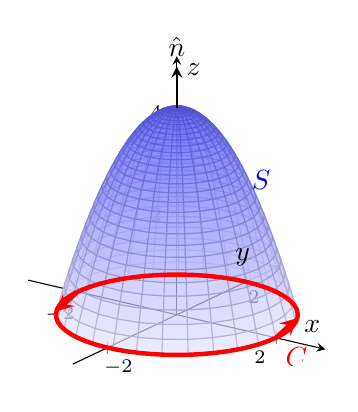
\begin{tikzpicture}
\begin{axis}[
    view={35}{25},
    width=8cm,
    height=7cm,
    xlabel={$x$},
    ylabel={$y$},
    zlabel={$z$},
    xmin=-3, xmax=3,
    ymin=-3, ymax=3,
    zmin=0, zmax=5,
    grid=major,
    axis lines=center,
    ticklabel style={font=\scriptsize}
]
% Paraboloid Surface S
\addplot3[
    surf,
    domain=0:360,
    y domain=0:2,
    samples=30,
    colormap={bluemap}{color=(blue!10) color=(blue!60)},
    opacity=0.7,
    z buffer=sort
]
({y*cos(x)}, {y*sin(x)}, {4 - y^2});

% Boundary Curve C
\addplot3[ultra thick, red, domain=0:360, samples=60, samples y=0] ({2*cos(x)}, {2*sin(x)}, {0});

% Arrows on C for counterclockwise orientation
\draw[-stealth, red, ultra thick] (axis cs:2,0,0) -- (axis cs:1.73,1,0);
\draw[-stealth, red, ultra thick] (axis cs:-2,0,0) -- (axis cs:-1.73,-1,0);

% Labels
\node[blue] at (axis cs:1,1,2.5) {$S$};
\node[red, below right] at (axis cs:2,0,0) {$C$};
\draw[-stealth, thick, black] (axis cs:0,0,4) -- (axis cs:0,0,4.8) node[above] {$\hat{n}$};
\end{axis}
\end{tikzpicture}
\end{center}

---

\textbf{2. Part I: Evaluating the Line Integral ($\oint_C \mathbf{F} \cdot d\mathbf{r}$)} \\
The boundary curve $C$ is the intersection of the paraboloid $z = 4 - x^2 - y^2$ with the $xy$-plane ($z = 0$). 
\begin{align*}
0 = 4 - x^2 - y^2 \implies x^2 + y^2 = 4
\end{align*}
This is a circle of radius $R = 2$ lying entirely in the plane $z = 0$. We parameterize this counterclockwise path using $t \in [0, 2\pi]$:
\begin{align*}
x &= 2\cos t \implies dx = -2\sin t \, dt \\
y &= 2\sin t \implies dy = 2\cos t \, dt \\
z &= 0 \implies dz = 0
\end{align*}
The vector field evaluated on the path becomes:
\begin{align*}
\mathbf{F}(x,y,z) &= 2z\mathbf{i} + x\mathbf{j} + y^2\mathbf{k} \\
&= 2(0)\mathbf{i} + (2\cos t)\mathbf{j} + (2\sin t)^2\mathbf{k} \\
&= 0\mathbf{i} + 2\cos t\mathbf{j} + 4\sin^2 t\mathbf{k}
\end{align*}
Now, substitute these elements into the line integral definition $\oint_C \mathbf{F} \cdot d\mathbf{r} = \oint_C (F_x \, dx + F_y \, dy + F_z \, dz)$:
\begin{align*}
\oint_C \mathbf{F} \cdot d\mathbf{r} &= \int_{0}^{2\pi} \left[ (0)(-2\sin t) + (2\cos t)(2\cos t) + (4\sin^2 t)(0) \right] dt \\
&= \int_{0}^{2\pi} 4\cos^2 t \, dt \\
&= 4 \int_{0}^{2\pi} \frac{1 + \cos(2t)}{2} \, dt \\
&= 2 \left[ t + \frac{\sin(2t)}{2} \right]_0^{2\pi} \\
&= 2 (2\pi + 0) - 2(0) \\
&= 4\pi
\end{align*}

---

\textbf{3. Part II: Evaluating the Surface Integral ($\iint_S (\nabla \times \mathbf{F}) \cdot \hat{n} \, dS$)} \\
First, we find the curl of the vector field $\mathbf{F} = 2z\mathbf{i} + x\mathbf{j} + y^2\mathbf{k}$:
\begin{align*}
\nabla \times \mathbf{F} &= \begin{vmatrix}
\mathbf{i} & \mathbf{j} & \mathbf{k} \\
\frac{\partial}{\partial x} & \frac{\partial}{\partial y} & \frac{\partial}{\partial z} \\
2z & x & y^2
\end{vmatrix} \\
&= \mathbf{i}\left( \frac{\partial}{\partial y}(y^2) - \frac{\partial}{\partial z}(x) \right) - \mathbf{j}\left( \frac{\partial}{\partial x}(y^2) - \frac{\partial}{\partial z}(2z) \right) + \mathbf{k}\left( \frac{\partial}{\partial x}(x) - \frac{\partial}{\partial y}(2z) \right) \\
&= \mathbf{i}(2y - 0) - \mathbf{j}(0 - 2) + \mathbf{k}(1 - 0) \\
&= 2y\mathbf{i} + 2\mathbf{j} + \mathbf{k}
\end{align*}

The surface $S$ is defined explicitly by $z = 4 - x^2 - y^2$. An upward-oriented differential normal element $\hat{n} \, dS$ is expressed as:
\begin{align*}
\hat{n} \, dS &= \left( -\frac{\partial z}{\partial x}\mathbf{i} - \frac{\partial z}{\partial y}\mathbf{j} + \mathbf{k} \right) dx \, dy
\end{align*}
Computing the partial derivatives:
\begin{align*}
\frac{\partial z}{\partial x} &= -2x \\
\frac{\partial z}{\partial y} &= -2y
\end{align*}
Substituting these yields:
\begin{align*}
\hat{n} \, dS &= (2x\mathbf{i} + 2y\mathbf{j} + \mathbf{k}) \, dx \, dy
\end{align*}

Now compute the dot product inside the surface integral:
\begin{align*}
(\nabla \times \mathbf{F}) \cdot \hat{n} \, dS &= (2y\mathbf{i} + 2\mathbf{j} + \mathbf{k}) \cdot (2x\mathbf{i} + 2y\mathbf{j} + \mathbf{k}) \, dx \, dy \\
&= (4xy + 4y + 1) \, dx \, dy
\end{align*}

The region of integration $R$ is the circular projection of the paraboloid onto the $xy$-plane, defined by $x^2 + y^2 \le 4$. We transform to polar coordinates ($x = r\cos\theta$, $y = r\sin\theta$, $dx \, dy = r \, dr \, d\theta$) over the limits $0 \le r \le 2$ and $0 \le \theta \le 2\pi$:
\begin{align*}
\iint_S (\nabla \times \mathbf{F}) \cdot \hat{n} \, dS &= \int_{0}^{2\pi} \int_{0}^{2} (4(r\cos\theta)(r\sin\theta) + 4r\sin\theta + 1) \, r \, dr \, d\theta \\
&= \int_{0}^{2\pi} \int_{0}^{2} (4r^3\sin\theta\cos\theta + 4r^2\sin\theta + r) \, dr \, d\theta
\end{align*}

Evaluate the inner integral with respect to $r$:
\begin{align*}
\int_{0}^{2} (4r^3\sin\theta\cos\theta + 4r^2\sin\theta + r) \, dr &= \left[ r^4\sin\theta\cos\theta + \frac{4}{3}r^3\sin\theta + \frac{r^2}{2} \right]_0^2 \\
&= 16\sin\theta\cos\theta + \frac{32}{3}\sin\theta + 2
\end{align*}

Now evaluate the outer integral with respect to $\theta$ over $[0, 2\pi]$:
\begin{align*}
\int_{0}^{2\pi} \left( 16\sin\theta\cos\theta + \frac{32}{3}\sin\theta + 2 \right) d\theta &= \left[ 8\sin^2\theta - \frac{32}{3}\cos\theta + 2\theta \right]_0^{2\pi} \\
&= \left( 0 - \frac{32}{3} + 4\pi \right) - \left( 0 - \frac{32}{3} + 0 \right) \\
&= 4\pi
\end{align*}

---

\textbf{4. Conclusion} \\
Since both calculations independently yield the identical value, Stokes' Theorem is successfully verified.
\begin{align*}
\boxed{\oint_C \mathbf{F} \cdot d\mathbf{r} = \iint_S (\nabla \times \mathbf{F}) \cdot \hat{n} \, dS = 4\pi}
\end{align*}

\end{tcolorbox}

\item State Stokes' theorem and verify it for $\mathbf{F}=(z^{2}-1)\mathbf{i}+(z+xy^{3})\mathbf{j}+6\mathbf{k}$ taken over the portion of $x=6-4y^{2}-4z^{2}$ in front of $x=-2$.
\mk{40} \yr{MATH 147 | L-1/T-2 | 2018--19}

\begin{tcolorbox}[enhanced,breakable,ansbox,colback=cD!4,colframe=cD,boxrule=0.8pt,arc=5pt,title={\textbf{Answer}},fonttitle=\bfseries\color{white},colbacktitle=cD]

\textbf{1. Statement of Stokes' Theorem} \\
Stokes' Theorem states that if $S$ is an oriented piecewise smooth surface bounded by a simple, closed, piecewise smooth boundary curve $C$ with positive (counterclockwise) orientation, and $\mathbf{F}$ is a vector field with continuous partial derivatives in an open region containing $S$, then:
\begin{align*}
\oint_C \mathbf{F} \cdot d\mathbf{r} &= \iint_S (\nabla \times \mathbf{F}) \cdot \hat{n} \, dS
\end{align*}

---

\textbf{2. Part I: Evaluating the Line Integral ($\oint_C \mathbf{F} \cdot d\mathbf{r}$)} \\
The boundary curve $C$ is formed by the intersection of the paraboloid $x = 6 - 4y^2 - 4z^2$ and the plane $x = -2$. Substituting $x = -2$ into the paraboloid equation gives:
\begin{align*}
-2 = 6 - 4y^2 - 4z^2 &\implies 4y^2 + 4z^2 = 8 \implies y^2 + z^2 = 2
\end{align*}
Thus, $C$ is a circle of radius $R = \sqrt{2}$ in the plane $x = -2$. Looking from the positive $x$-axis, we parameterize this counterclockwise path using $t \in [0, 2\pi]$:
\begin{align*}
x &= -2 \implies dx = 0 \\
y &= \sqrt{2}\cos t \implies dy = -\sqrt{2}\sin t \, dt \\
z &= \sqrt{2}\sin t \implies dz = \sqrt{2}\cos t \, dt
\end{align*}

Substitute these into the components of the vector field $\mathbf{F} = (z^2-1)\mathbf{i} + (z+xy^3)\mathbf{j} + 6\mathbf{k}$:
\begin{align*}
F_x &= (\sqrt{2}\sin t)^2 - 1 = 2\sin^2 t - 1 \\
F_y &= \sqrt{2}\sin t + (-2)(\sqrt{2}\cos t)^3 = \sqrt{2}\sin t - 4\sqrt{2}\cos^3 t \\
F_z &= 6
\end{align*}

The line integral becomes:
\begin{align*}
\oint_C \mathbf{F} \cdot d\mathbf{r} &= \int_{0}^{2\pi} \left( F_x\,dx + F_y\,dy + F_z\,dz \right) \\
&= \int_{0}^{2\pi} \left[ 0 + \left(\sqrt{2}\sin t - 4\sqrt{2}\cos^3 t\right)\left(-\sqrt{2}\sin t\right) + 6\left(\sqrt{2}\cos t\right) \right] dt \\
&= \int_{0}^{2\pi} \left( -2\sin^2 t + 8\sin t\cos^3 t + 6\sqrt{2}\cos t \right) dt
\end{align*}

Evaluating each term over the period $[0, 2\pi]$:
\begin{itemize}
    \item $\displaystyle\int_{0}^{2\pi} -2\sin^2 t \, dt = -2\left(\frac{2\pi}{2}\right) = -2\pi$
    \item $\displaystyle\int_{0}^{2\pi} 8\sin t\cos^3 t \, dt = \left[ -2\cos^4 t \right]_0^{2\pi} = -2(1 - 1) = 0$
    \item $\displaystyle\int_{0}^{2\pi} 6\sqrt{2}\cos t \, dt = \left[ 6\sqrt{2}\sin t \right]_0^{2\pi} = 0$
\end{itemize}
Summing these values, the line integral evaluates to:
\begin{align*}
\oint_C \mathbf{F} \cdot d\mathbf{r} &= -2\pi
\end{align*}

---

\textbf{3. Part II: Evaluating the Surface Integral ($\iint_S (\nabla \times \mathbf{F}) \cdot \hat{n} \, dS$)} \\
First, we find the curl of $\mathbf{F}$:
\begin{align*}
\nabla \times \mathbf{F} &= \begin{vmatrix}
\mathbf{i} & \mathbf{j} & \mathbf{k} \\
\frac{\partial}{\partial x} & \frac{\partial}{\partial y} & \frac{\partial}{\partial z} \\
z^2-1 & z+xy^3 & 6
\end{vmatrix} \\
&= \mathbf{i}\left( 0 - 1 \right) - \mathbf{j}\left( 0 - 2z \right) + \mathbf{k}\left( y^3 - 0 \right) \\
&= -\mathbf{i} + 2z\mathbf{j} + y^3\mathbf{k}
\end{align*}

The surface is given explicitly as $x = 6 - 4y^2 - 4z^2$. Since the boundary curve is traversed counterclockwise when viewed from the positive $x$-axis, the surface normal must point forward (in the positive $x$-direction). The differential normal vector element $\hat{n} \, dS$ is:
\begin{align*}
\hat{n} \, dS &= \left( \mathbf{i} - \frac{\partial x}{\partial y}\mathbf{j} - \frac{\partial x}{\partial z}\mathbf{k} \right) dy \, dz
\end{align*}
Computing the partial derivatives: $\frac{\partial x}{\partial y} = -8y$ and $\frac{\partial x}{\partial z} = -8z$. This gives:
\begin{align*}
\hat{n} \, dS &= (\mathbf{i} + 8y\mathbf{j} + 8z\mathbf{k}) \, dy \, dz
\end{align*}

Now, compute the inner dot product:
\begin{align*}
(\nabla \times \mathbf{F}) \cdot \hat{n} \, dS &= (-\mathbf{i} + 2z\mathbf{j} + y^3\mathbf{k}) \cdot (\mathbf{i} + 8y\mathbf{j} + 8z\mathbf{k}) \, dy \, dz \\
&= (-1 + 16yz + 8zy^3) \, dy \, dz
\end{align*}

The projection region $D$ on the $yz$-plane is the disk $y^2 + z^2 \le 2$. Converting to polar coordinates where $y = r\cos\theta$ and $z = r\sin\theta$ over $0 \le r \le \sqrt{2}$ and $0 \le \theta \le 2\pi$:
\begin{align*}
\iint_S (\nabla \times \mathbf{F}) \cdot \hat{n} \, dS &= \int_{0}^{2\pi} \int_{0}^{\sqrt{2}} (-1 + 16r^2\sin\theta\cos\theta + 8r^4\sin\theta\cos^3\theta) \, r \, dr \, d\theta \\
&= \int_{0}^{2\pi} \int_{0}^{\sqrt{2}} (-r + 16r^3\sin\theta\cos\theta + 8r^5\sin\theta\cos^3\theta) \, dr \, d\theta
\end{align*}

Integrating with respect to $\theta$ first over $[0, 2\pi]$, notice that the symmetric periodic components containing $\sin\theta$ evaluate to zero:
\begin{align*}
\int_{0}^{2\pi} \sin\theta\cos\theta \, d\theta &= 0 \\
\int_{0}^{2\pi} \sin\theta\cos^3\theta \, d\theta &= 0
\end{align*}

Thus, the remaining non-zero portion reduces to:
\begin{align*}
\int_{0}^{2\pi} \int_{0}^{\sqrt{2}} -r \, dr \, d\theta &= \left( \int_{0}^{2\pi} d\theta \right) \left( \int_{0}^{\sqrt{2}} -r \, dr \right) \\
&= (2\pi) \left[ -\frac{r^2}{2} \right]_0^{\sqrt{2}} \\
&= 2\pi \left( -\frac{2}{2} \right) = -2\pi
\end{align*}

---

\textbf{4. Conclusion} \\
Since both the line integral and surface integral yield exactly $-2\pi$, Stokes' Theorem is verified.
\begin{align*}
\boxed{ \oint_C \mathbf{F} \cdot d\mathbf{r} = \iint_S (\nabla \times \mathbf{F}) \cdot \hat{n} \, dS = -2\pi }
\end{align*}

\end{tcolorbox}

\item Evaluate $\displaystyle\iint(\nabla\times\mathbf{A})\cdot\hat{n}\,dS$ where $\mathbf{A}=(x^{2}+y-4)\mathbf{i}+3xy\mathbf{j}+(2xz+z^{2})\mathbf{k}$ and $S$ is the surface of the hemisphere $x^{2}+y^{2}+z^{2}=16$ above the $xy$-plane.
\mk{26} \yr{MATH 147 | L-1/T-2 | 2015--16}

\begin{tcolorbox}[enhanced,breakable,ansbox,colback=cD!4,colframe=cD,boxrule=0.8pt,arc=5pt,title={\textbf{Answer}},fonttitle=\bfseries\color{white},colbacktitle=cD]

\textbf{1. Applying Stokes' Theorem} \\
Instead of evaluating the surface integral directly, we can apply **Stokes' Theorem**, which states:
\begin{align*}
\iint_{S} (\nabla \times \mathbf{A}) \cdot \hat{n} \, dS &= \oint_{C} \mathbf{A} \cdot d\mathbf{r}
\end{align*}
where $C$ is the boundary curve of the hemisphere $S$ lying in the $xy$-plane, oriented counterclockwise when viewed from above.



\textbf{2. Parameterizing the Boundary Curve $C$} \\
The hemisphere is defined by $x^2 + y^2 + z^2 = 16$ for $z \ge 0$. The boundary curve $C$ occurs where the surface meets the $xy$-plane ($z = 0$):
\begin{align*}
x^2 + y^2 + 0^2 = 16 \implies x^2 + y^2 = 16
\end{align*}
This is a circle of radius $R = 4$ centered at the origin in the plane $z = 0$. We can parameterize $C$ with parameter $t \in [0, 2\pi]$ as follows:
\begin{align*}
x &= 4\cos t \implies dx = -4\sin t \, dt \\
y &= 4\sin t \implies dy = 4\cos t \, dt \\
z &= 0 \implies dz = 0
\end{align*}

\textbf{3. Setting up the Line Integral} \\
We rewrite the vector field $\mathbf{A} = (x^{2}+y-4)\mathbf{i} + 3xy\mathbf{j} + (2xz+z^{2})\mathbf{k}$ along the curve $C$ by substituting $z = 0$:
\begin{align*}
\mathbf{A} &= (x^2 + y - 4)\mathbf{i} + 3xy\mathbf{j} + 0\mathbf{k}
\end{align*}
The line integral can be expanded into its differential components:
\begin{align*}
\oint_{C} \mathbf{A} \cdot d\mathbf{r} &= \int_{0}^{2\pi} \left[ (x^2 + y - 4)\,dx + 3xy\,dy \right]
\end{align*}

Substitute the parameterized values of $x$, $y$, $dx$, and $dy$:
\begin{align*}
\oint_{C} \mathbf{A} \cdot d\mathbf{r} &= \int_{0}^{2\pi} \left[ \left(16\cos^2 t + 4\sin t - 4\right)(-4\sin t) + 3(4\cos t)(4\sin t)(4\cos t) \right] dt \\
&= \int_{0}^{2\pi} \left[ -64\cos^2 t\sin t - 16\sin^2 t + 16\sin t + 192\cos^2 t\sin t \right] dt \\
&= \int_{0}^{2\pi} \left[ 128\cos^2 t\sin t - 16\sin^2 t + 16\sin t \right] dt
\end{align*}

\textbf{4. Evaluating the Integral} \\
We can compute the integral term by term over the interval $[0, 2\pi]$:

\begin{itemize}
    \item \textbf{First Term:} $\displaystyle\int_{0}^{2\pi} 128\cos^2 t\sin t \, dt$ \\
    Using substitution $u = \cos t \implies du = -\sin t \, dt$. The limits change from $t=0 \to u=1$ and $t=2\pi \to u=1$. Since the lower and upper limits are equal:
    \begin{align*}
    \int_{1}^{1} -128u^2 \, du &= 0
    \end{align*}

    \item \textbf{Second Term:} $\displaystyle\int_{0}^{2\pi} -16\sin^2 t \, dt$ \\
    Using the half-angle identity $\sin^2 t = \frac{1 - \cos(2t)}{2}$:
    \begin{align*}
    -16 \int_{0}^{2\pi} \frac{1 - \cos(2t)}{2} \, dt &= -8 \left[ t - \frac{\sin(2t)}{2} \right]_0^{2\pi} \\
    &= -8(2\pi - 0) = -16\pi
    \end{align*}

    \item \textbf{Third Term:} $\displaystyle\int_{0}^{2\pi} 16\sin t \, dt$ \\
    Integrating $\sin t$ over a full period $[0, 2\pi]$ results in zero:
    \begin{align*}
    \left[ -16\cos t \right]_0^{2\pi} &= -16(1 - 1) = 0
    \end{align*}
\end{itemize}

Summing up the values of the three terms:
\begin{align*}
\oint_{C} \mathbf{A} \cdot d\mathbf{r} &= 0 - 16\pi + 0 = -16\pi
\end{align*}

\vspace{1em}
\textbf{Final Answer:}
\begin{align*}
\boxed{ \iint_{S} (\nabla \times \mathbf{A}) \cdot \hat{n} \, dS = -16\pi }
\end{align*}

\end{tcolorbox}

\end{enumerate}


%% ══════════════════════════════════════════════════════════════════════
%%  PART V — COMPLEX CALCULUS
%% ══════════════════════════════════════════════════════════════════════
\secdivider{Complex Calculus}{Analytic Functions, Cauchy-Riemann, Complex Integration}{cE}


\section{S5. Complex Calculus}
\label{sec:S5}
\markboth{S5. Complex Calculus}{}

%%──────────────────────────────────────────────────────────────────────
\subtopic{cE}{Geometry of Complex Numbers}
\label{sub:s5-geometry}

\begin{enumerate}
    
\item Find the bilinear transformation which maps $z_{1}=-i$, $z_{2}=0$, $z_{3}=i$ into $w_{1}=-1$, $w_{2}=i$, $w_{3}=1$. Hence find the image of the $y$-axis.
\mk{10} \yr{MATH 241 | L-2/T-1 | 2024--25}

\begin{tcolorbox}[enhanced,breakable,ansbox,colback=cE!4,colframe=cE,boxrule=0.8pt,arc=5pt,title={\textbf{Answer}},fonttitle=\bfseries\color{white},colbacktitle=cE]

\textbf{1. Finding the Bilinear Transformation}

The bilinear (or Möbius) transformation that maps three distinct points $z_1, z_2, z_3$ in the $z$-plane to three distinct points $w_1, w_2, w_3$ in the $w$-plane preserves the cross-ratio. The implicit equation is given by:
\begin{equation}
    \frac{(w - w_1)(w_2 - w_3)}{(w - w_2)(w_1 - w_3)} = \frac{(z - z_1)(z_2 - z_3)}{(z - z_2)(z_1 - z_3)}
\end{equation}

Given the mappings:
\begin{align*}
    z_1 &= -i & w_1 &= -1 \\
    z_2 &= 0 & w_2 &= i \\
    z_3 &= i & w_3 &= 1
\end{align*}

Substitute these values into the cross-ratio formula:
\begin{align*}
    \frac{(w - (-1))(i - 1)}{(w - i)(-1 - 1)} &= \frac{(z - (-i))(0 - i)}{(z - 0)(-i - i)} \\[1em]
    \frac{(w + 1)(i - 1)}{-2(w - i)} &= \frac{(z + i)(-i)}{z(-2i)}
\end{align*}

Simplify the right-hand side:
\begin{equation*}
    \frac{(w + 1)(i - 1)}{-2(w - i)} = \frac{z + i}{2z}
\end{equation*}

Multiply both sides by $-2$:
\begin{equation*}
    \frac{(w + 1)(i - 1)}{w - i} = \frac{-(z + i)}{z}
\end{equation*}

Cross-multiply to solve for $w$:
\begin{align*}
    z(i - 1)(w + 1) &= -(w - i)(z + i) \\
    wz(i - 1) + z(i - 1) &= - (wz + wi - iz - i^2) \\
    wzi - wz + zi - z &= -wz - wi + iz - 1
\end{align*}

Bring all terms involving $w$ to the left side and the rest to the right side:
\begin{align*}
    wzi - wz + wz + wi &= -iz + iz + z - 1 \\
    wzi + wi &= z - 1 \\
    w(zi + i) &= z - 1 \\
    wi(z + 1) &= z - 1
\end{align*}

Divide by $i(z+1)$ to isolate $w$:
\begin{equation*}
    w = \frac{z - 1}{i(z + 1)} = -i \left( \frac{z - 1}{z + 1} \right)
\end{equation*}
\begin{equation*}
    \boxed{w = \frac{-iz + i}{z + 1}}
\end{equation*}

\vspace{0.5cm}
\textbf{2. Finding the Image of the $y$-axis}

The $y$-axis in the $z$-plane is the imaginary axis, which consists of all points where $\text{Re}(z) = 0$, or $z = iy$ for $y \in \mathbb{R}$.

\textit{Method 1: Using properties of bilinear transformations}\\
A bilinear transformation maps circles and lines in the $z$-plane to circles and lines in the $w$-plane. The $y$-axis is a line passing through $z_1 = -i$, $z_2 = 0$, and $z_3 = i$. Their respective images are $w_1 = -1$, $w_2 = i$, and $w_3 = 1$. The unique circle passing through $-1, i$, and $1$ in the $w$-plane is the unit circle, $|w| = 1$. Therefore, the image of the $y$-axis is the unit circle.

\textit{Method 2: Analytical verification}\\
Let $z = iy$. Substitute this into the transformation:
\begin{equation*}
    w = -i \left( \frac{iy - 1}{iy + 1} \right)
\end{equation*}
Calculate the magnitude of $w$:
\begin{equation*}
    |w| = |-i| \cdot \left| \frac{-1 + iy}{1 + iy} \right| = 1 \cdot \frac{\sqrt{(-1)^2 + y^2}}{\sqrt{1^2 + y^2}} = \frac{\sqrt{1 + y^2}}{\sqrt{1 + y^2}} = 1
\end{equation*}
Thus, for any point on the $y$-axis, its image satisfies $|w| = 1$.

\begin{equation*}
    \boxed{\text{The image of the } y\text{-axis is the unit circle } |w| = 1 \text{ in the } w\text{-plane.}}
\end{equation*}

\vspace{0.5cm}
\begin{center}
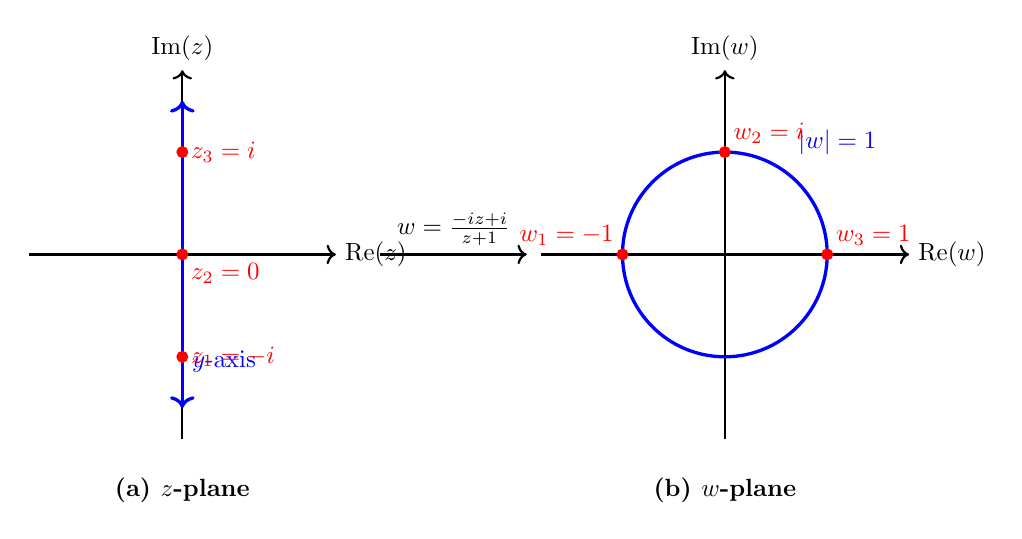
\begin{tikzpicture}[scale=1.3, every node/.style={scale=0.9}]
    % Z-plane
    \draw[->, thick] (-1.5,0) -- (1.5,0) node[right] {$\text{Re}(z)$};
    \draw[->, thick] (0,-1.8) -- (0,1.8) node[above] {$\text{Im}(z)$};
    \draw[very thick, blue, <->] (0,-1.5) -- (0,1.5) node[pos=0.15, right] {$y$-axis};
    
    \filldraw[red] (0,-1) circle (1.5pt) node[right] {$z_1 = -i$};
    \filldraw[red] (0,0) circle (1.5pt) node[anchor=north west] {$z_2 = 0$};
    \filldraw[red] (0,1) circle (1.5pt) node[right] {$z_3 = i$};
    \node at (0,-2.3) {\textbf{(a) $z$-plane}};

    % Mapping arrow
    \draw[->, thick, shorten >= 5pt, shorten <= 5pt] (1.8,0) -- (3.5,0) node[midway, above] {$w = \frac{-iz+i}{z+1}$};

    % W-plane
    \begin{scope}[xshift=5.3cm]
        \draw[->, thick] (-1.8,0) -- (1.8,0) node[right] {$\text{Re}(w)$};
        \draw[->, thick] (0,-1.8) -- (0,1.8) node[above] {$\text{Im}(w)$};
        
        \draw[very thick, blue] (0,0) circle (1);
        \node[blue] at (1.1,1.1) {$|w|=1$};
        
        \filldraw[red] (-1,0) circle (1.5pt) node[above left] {$w_1 = -1$};
        \filldraw[red] (0,1) circle (1.5pt) node[above right] {$w_2 = i$};
        \filldraw[red] (1,0) circle (1.5pt) node[above right] {$w_3 = 1$};
        \node at (0,-2.3) {\textbf{(b) $w$-plane}};
    \end{scope}
\end{tikzpicture}
\end{center}

\end{tcolorbox}

\item Find all values of $z$ for which $z^{5}=-32$, and locate these values in the complex plane.
\mk{10} \yr{MATH 241 | L-2/T-1 | 2023--24}

\begin{tcolorbox}[enhanced,breakable,ansbox,colback=cE!4,colframe=cE,boxrule=0.8pt,arc=5pt,title={\textbf{Answer}},fonttitle=\bfseries\color{white},colbacktitle=cE]

To find all values of $z$ satisfying the equation $z^5 = -32$, we can utilize the polar form of complex numbers and De Moivre's Theorem.

\subsection*{1. Finding the Roots}

First, we express the complex number $-32$ in its polar (exponential) form. The magnitude is $|-32| = 32$, and its argument lies on the negative real axis, which corresponds to $\pi$ radians. To find all unique roots, we include the periodic forms:
\[
-32 = 32 e^{i(\pi + 2k\pi)} = 32 \exp\left(i \pi (2k + 1)\right) \quad \text{for } k \in \mathbb{Z}
\]

Taking the fifth root on both sides yields the general expression for $z$:
\[
z_k = (32)^{1/5} \exp\left(i \frac{(2k + 1)\pi}{5}\right) = 2 \exp\left(i \frac{(2k + 1)\pi}{5}\right)
\]
By choosing $k = 0, 1, 2, 3, 4$, we obtain the five distinct roots:

\begin{align*}
    k = 0: \quad z_0 &= 2 e^{i\pi/5} = 2\left(\cos\frac{\pi}{5} + i\sin\frac{\pi}{5}\right) \\
    k = 1: \quad z_1 &= 2 e^{i3\pi/5} = 2\left(\cos\frac{3\pi}{5} + i\sin\frac{3\pi}{5}\right) \\
    k = 2: \quad z_2 &= 2 e^{i5\pi/5} = 2 e^{i\pi} = -2 \\
    k = 3: \quad z_3 &= 2 e^{i7\pi/5} = 2\left(\cos\frac{7\pi}{5} + i\sin\frac{7\pi}{5}\right) \\
    k = 4: \quad z_4 &= 2 e^{i9\pi/5} = 2\left(\cos\frac{9\pi}{5} + i\sin\frac{9\pi}{5}\right)
\end{align*}

Thus, the complete set of solutions is:
\[
\boxed{z_k = 2 \left( \cos\frac{(2k+1)\pi}{5} + i\sin\frac{(2k+1)\pi}{5} \right) \quad \text{for } k = 0, 1, 2, 3, 4}
\]

\subsection*{2. Location in the Complex Plane}

Geometrically, these five roots lie on a circle centered at the origin with a radius of $R = 2$. They form the vertices of a regular pentagon, spaced symmetrically at equal angular intervals of $\Delta \theta = \frac{2\pi}{5} = 72^\circ$, starting from the initial angle $\theta_0 = \frac{\pi}{5} = 36^\circ$.

\begin{center}
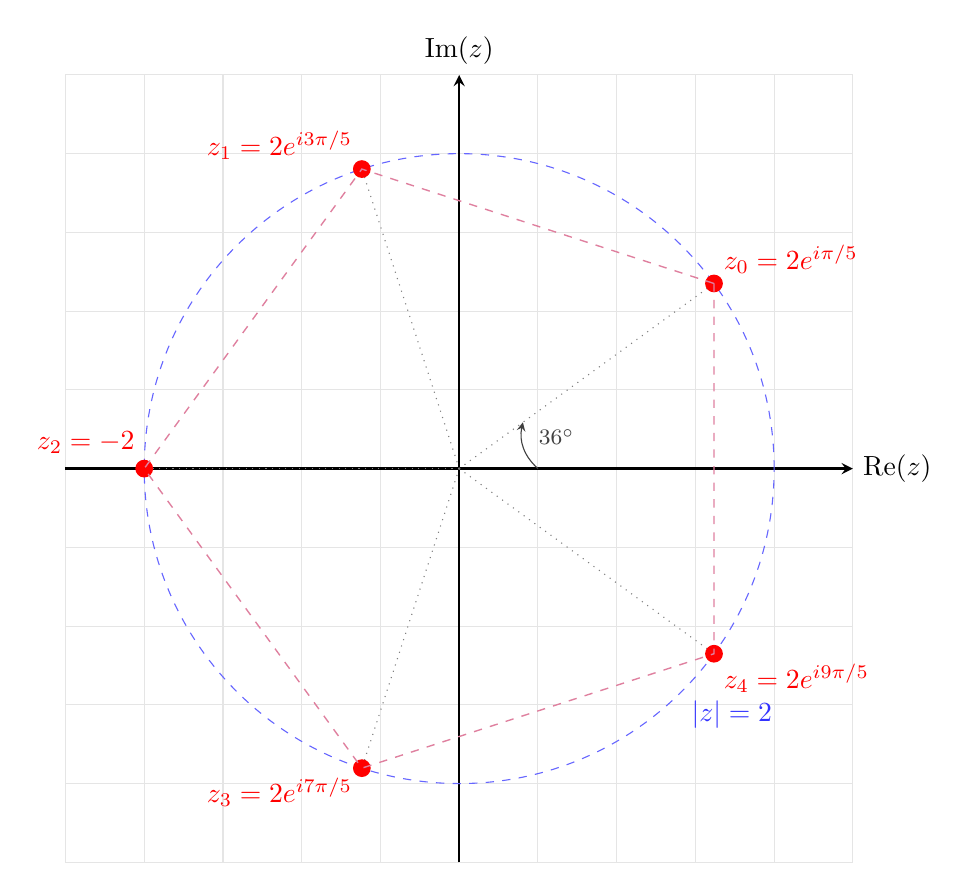
\begin{tikzpicture}[scale=2.0, >=stealth]
    % Grid lines (optional, clean look)
    \draw[color=gray!20, thin, step=0.5] (-2.5,-2.5) grid (2.5,2.5);
    
    % Axes
    \draw[->, thick] (-2.5,0) -- (2.5,0) node[right] {$\text{Re}(z)$};
    \draw[->, thick] (0,-2.5) -- (0,2.5) node[above] {$\text{Im}(z)$};
    
    % Circle of radius 2
    \draw[dashed, blue!60, thin] (0,0) circle (2);
    \node[blue!80, anchor=north west] at (1.414,-1.414) {$|z|=2$};
    
    % Radial lines and Roots
    % z_0 (36 degrees)
    \draw[dotted, gray] (0,0) -- (36:2);
    \filldraw[red] (36:2) circle (1.5pt) node[anchor=south west] {$z_0 = 2e^{i\pi/5}$};
    
    % z_1 (108 degrees)
    \draw[dotted, gray] (0,0) -- (108:2);
    \filldraw[red] (108:2) circle (1.5pt) node[anchor=south east] {$z_1 = 2e^{i3\pi/5}$};
    
    % z_2 (180 degrees)
    \draw[dotted, gray] (0,0) -- (180:2);
    \filldraw[red] (180:2) circle (1.5pt) node[anchor=south east, yshift=2pt] {$z_2 = -2$};
    
    % z_3 (252 degrees)
    \draw[dotted, gray] (0,0) -- (252:2);
    \filldraw[red] (252:2) circle (1.5pt) node[anchor=north east] {$z_3 = 2e^{i7\pi/5}$};
    
    % z_4 (324 degrees)
    \draw[dotted, gray] (0,0) -- (324:2);
    \filldraw[red] (324:2) circle (1.5pt) node[anchor=north west] {$z_4 = 2e^{i9\pi/5}$};
    
    % Outer Polygon connecting roots
    \draw[line width=0.5pt, draw=purple!50, dashed] (36:2) -- (108:2) -- (180:2) -- (252:2) -- (324:2) -- cycle;
    
    % Label specific angle for z_0
    \draw[->, bend left=20, darkgray, thin] (0.5,0) to [bend left=30] (36:0.5);
    \node[darkgray] at (18:0.65) {\footnotesize $36^\circ$};

\end{tikzpicture}
\end{center}

\end{tcolorbox}

\item Find the image of $\operatorname{Im}(z)\ge 0$ under the transformation $w=\dfrac{z-i}{iz-1}$. Sketch the region $\operatorname{Im}(z)\ge 0$ and its image.
\mk{8} \yr{MATH 241 | L-2/T-1 | 2022--23}

\begin{tcolorbox}[enhanced,breakable,ansbox,colback=cE!4,colframe=cE,boxrule=0.8pt,arc=5pt,title={\textbf{Answer}},fonttitle=\bfseries\color{white},colbacktitle=cE]

To find the image of the region $\operatorname{Im}(z) \ge 0$ under the bilinear transformation 
\[
w = \frac{z - i}{iz - 1}
\]
we analyze how the mapping behaves both on the boundary ($\operatorname{Im}(z) = 0$) and in the interior ($\operatorname{Im}(z) > 0$).

\subsection*{1. Analytical Derivation}

Let $z = x + iy$, where $x, y \in \mathbb{R}$. The given region is $\operatorname{Im}(z) = y \ge 0$. Let us compute the magnitude squared of $w$, $|w|^2 = w\bar{w}$:

\[
|w|^2 = \left| \frac{z - i}{iz - 1} \right|^2 = \frac{|z - i|^2}{|iz - 1|^2}
\]

Expanding the numerator and the denominator in terms of $x$ and $y$:
\begin{align*}
|z - i|^2 &= |x + i(y - 1)|^2 = x^2 + (y - 1)^2 = x^2 + y^2 - 2y + 1 \\[0.5em]
|iz - 1|^2 &= |i(x + iy) - 1|^2 = |-y - 1 + ix|^2 = (-y - 1)^2 + x^2 = x^2 + y^2 + 2y + 1
\end{align*}

Now, let us find the difference $|w|^2 - 1$:
\begin{align*}
|w|^2 - 1 &= \frac{|z - i|^2 - |iz - 1|^2}{|iz - 1|^2} \\[0.5em]
&= \frac{(x^2 + y^2 - 2y + 1) - (x^2 + y^2 + 2y + 1)}{|iz - 1|^2} \\[0.5em]
&= \frac{-4y}{|iz - 1|^2} = \frac{-4\operatorname{Im}(z)}{|iz - 1|^2}
\end{align*}

We are given the region $\operatorname{Im}(z) \ge 0$. Substituting this condition into our relation:
\[
\operatorname{Im}(z) \ge 0 \implies -4\operatorname{Im}(z) \le 0 \implies |w|^2 - 1 \le 0 \implies |w|^2 \le 1
\]

Taking the square root since magnitudes are non-negative, we obtain:
\[
\boxed{|w| \le 1}
\]

Thus, the transformation maps the upper half of the $z$-plane (including the real axis) onto the **closed unit disk** in the $w$-plane.

---

\subsection*{2. Boundary Mapping Verification}
To confirm, we can check where specific points on the boundary line $\operatorname{Im}(z) = 0$ (the real axis) map to in the $w$-plane:
* For $z = 0$: $w = \frac{-i}{-1} = i$
* For $z = 1$: $w = \frac{1 - i}{i - 1} = -1$
* For $z = -1$: $w = \frac{-1 - i}{-i - 1} = 1$
* For $z = \infty$: $w = \frac{1}{i} = -i$

All these image points ($i, -1, 1, -i$) lie on the boundary circle $|w| = 1$. Testing an interior point like $z = i$ ($\operatorname{Im}(z) > 0$) yields $w = \frac{i - i}{i^2 - 1} = 0$, confirming the interior maps inside the unit disk.

---

\subsection*{3. Graphical Representation}

\begin{center}
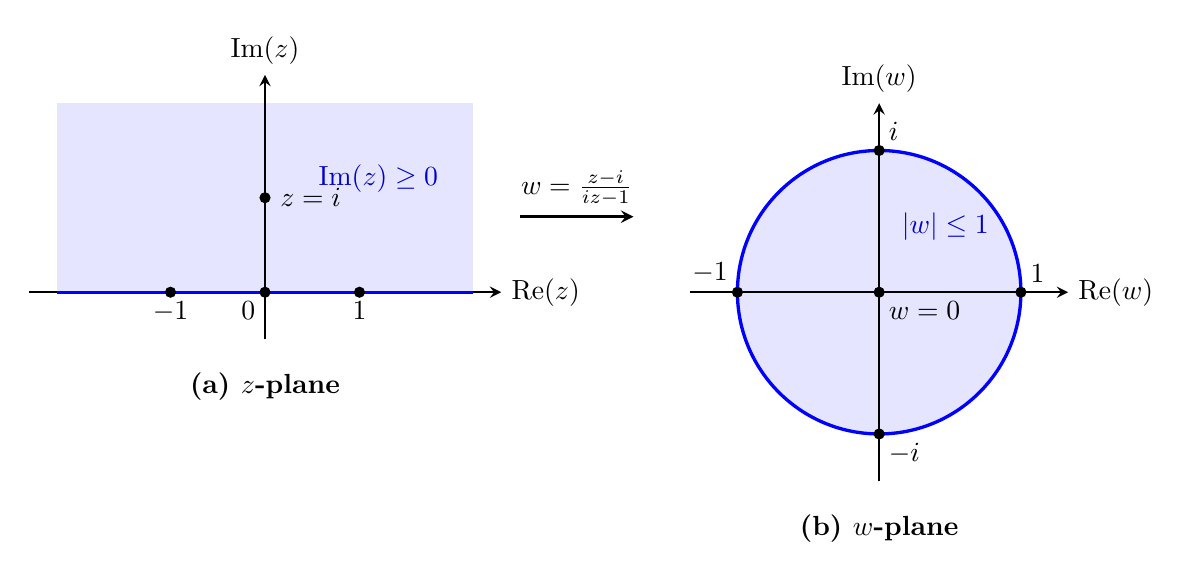
\begin{tikzpicture}[scale=1.2, >=stealth]

    % ================= z-plane =================
    \begin{scope}[xshift=-3cm]
        % Shading the upper half plane
        \fill[blue!10] (-2.2,0) rectangle (2.2,2.0);
        
        % Axes
        \draw[->, thick] (-2.5,0) -- (2.5,0) node[right] {$\text{Re}(z)$};
        \draw[->, thick] (0,-0.5) -- (0,2.3) node[above] {$\text{Im}(z)$};
        
        % Solid boundary line for Im(z) >= 0
        \draw[very thick, blue] (-2.2,0) -- (2.2,0);
        
        % Test points
        \filldraw[black] (0,1) circle (1.5pt) node[right, xshift=2pt] {$z = i$};
        \filldraw[black] (0,0) circle (1.5pt) node[below left] {$0$};
        \filldraw[black] (1,0) circle (1.5pt) node[below] {$1$};
        \filldraw[black] (-1,0) circle (1.5pt) node[below] {$-1$};
        
        % Region Label
        \node[blue!80!black] at (1.2,1.2) {$\operatorname{Im}(z) \ge 0$};
        \node at (0,-1.0) {\textbf{(a) $z$-plane}};
    \end{scope}

    % ================= Mapping Arrow =================
    \draw[->, line width=1pt] (-0.3,0.8) -- (0.9,0.8) node[midway, above] {$w = \frac{z-i}{iz-1}$};

    % ================= w-plane =================
    \begin{scope}[xshift=3.5cm]
        % Shading the disk
        \fill[blue!10] (0,0) circle (1.5);
        
        % Axes
        \draw[->, thick] (-2.0,0) -- (2.0,0) node[right] {$\text{Re}(w)$};
        \draw[->, thick] (0,-2.0) -- (0,2.0) node[above] {$\text{Im}(w)$};
        
        % Boundary Circle
        \draw[very thick, blue] (0,0) circle (1.5);
        
        % Mapped points (scaled by 1.5 for visualization)
        \filldraw[black] (0,0) circle (1.5pt) node[below right] {$w = 0$};
        \filldraw[black] (0,1.5) circle (1.5pt) node[above right] {$i$};
        \filldraw[black] (-1.5,0) circle (1.5pt) node[above left] {$-1$};
        \filldraw[black] (1.5,0) circle (1.5pt) node[above right] {$1$};
        \filldraw[black] (0,-1.5) circle (1.5pt) node[below right] {$-i$};
        
        % Region Label
        \node[blue!80!black] at (0.7,0.7) {$|w| \le 1$};
        \node at (0,-2.5) {\textbf{(b) $w$-plane}};
    \end{scope}

\end{tikzpicture}
\end{center}

\end{tcolorbox}

\item Show that $\operatorname{Log}(-1+i\sqrt{3})^{2}\neq 2\operatorname{Log}(-1+i\sqrt{3})$.
\mk{6} \yr{MATH 241 | L-2/T-1 | 2022--23, 2016--17, 2015--16}

\begin{tcolorbox}[enhanced,breakable,ansbox,colback=cE!4,colframe=cE,boxrule=0.8pt,arc=5pt,title={\textbf{Answer}},fonttitle=\bfseries\color{white},colbacktitle=cE]

To show that $\operatorname{Log}\left((-1+i\sqrt{3})^2\right) \neq 2\operatorname{Log}(-1+i\sqrt{3})$, we evaluate the Left-Hand Side (LHS) and the Right-Hand Side (RHS) individually using the definition of the principal branch of the complex logarithm:
\[
\operatorname{Log}(z) = \ln|z| + i\operatorname{Arg}(z) \quad \text{where } \operatorname{Arg}(z) \in (-\pi, \pi]
\]

Let $z = -1 + i\sqrt{3}$.

\subsection*{1. Evaluating the Right-Hand Side: $2\operatorname{Log}(z)$}

First, find the magnitude and principal argument of $z = -1 + i\sqrt{3}$:
\[
|z| = \sqrt{(-1)^2 + (\sqrt{3})^2} = \sqrt{1 + 3} = 2
\]
Since $z$ lies in the second quadrant ($\text{Re}(z) < 0$ and $\text{Im}(z) > 0$), its principal argument is:
\[
\operatorname{Arg}(z) = \pi - \tan^{-1}\left(\frac{\sqrt{3}}{1}\right) = \pi - \frac{\pi}{3} = \frac{2\pi}{3}
\]

Now, compute $\operatorname{Log}(z)$:
\[
\operatorname{Log}(z) = \ln(2) + i\frac{2\pi}{3}
\]
Multiplying by 2 gives the RHS:
\begin{equation}
2\operatorname{Log}(z) = 2\ln(2) + i\frac{4\pi}{3}
\end{equation}

\subsection*{2. Evaluating the Left-Hand Side: $\operatorname{Log}(z^2)$}

First, compute $z^2$:
\[
z^2 = (-1 + i\sqrt{3})^2 = 1 - 3 - 2i\sqrt{3} = -2 - 2i\sqrt{3}
\]
Next, find the magnitude and principal argument of $z^2 = -2 - 2i\sqrt{3}$:
\[
|z^2| = \sqrt{(-2)^2 + (-2\sqrt{3})^2} = \sqrt{4 + 12} = 4
\]
Since $z^2$ lies in the third quadrant ($\text{Re}(z^2) < 0$ and $\text{Im}(z^2) < 0$), its principal argument must lie within the interval $(-\pi, \pi]$:
\[
\operatorname{Arg}(z^2) = -\pi + \tan^{-1}\left(\frac{-2\sqrt{3}}{-2}\right) = -\pi + \frac{\pi}{3} = -\frac{2\pi}{3}
\]

Now, compute $\operatorname{Log}(z^2)$:
\begin{equation}
\operatorname{Log}(z^2) = \ln(4) + i\left(-\frac{2\pi}{3}\right) = 2\ln(2) - i\frac{2\pi}{3}
\end{equation}

\subsection*{3. Conclusion}

Comparing equation (1) and equation (2):
\[
\text{LHS} = 2\ln(2) - i\frac{2\pi}{3} \quad \neq \quad \text{RHS} = 2\ln(2) + i\frac{4\pi}{3}
\]
The values are distinct because their imaginary parts differ by $2\pi$, which occurs because the doubled angle crosses the branch cut along the negative real axis. Thus, we have shown that:
\[
\boxed{\operatorname{Log}(-1+i\sqrt{3})^{2} \neq 2\operatorname{Log}(-1+i\sqrt{3})}
\]

\subsection*{Geometrical Visualization}

The diagram below illustrates how doubling the argument of $z$ crosses the branch cut (the negative real axis), causing the principal argument $\operatorname{Arg}(z^2)$ to wrap around to a negative angle.

\begin{center}
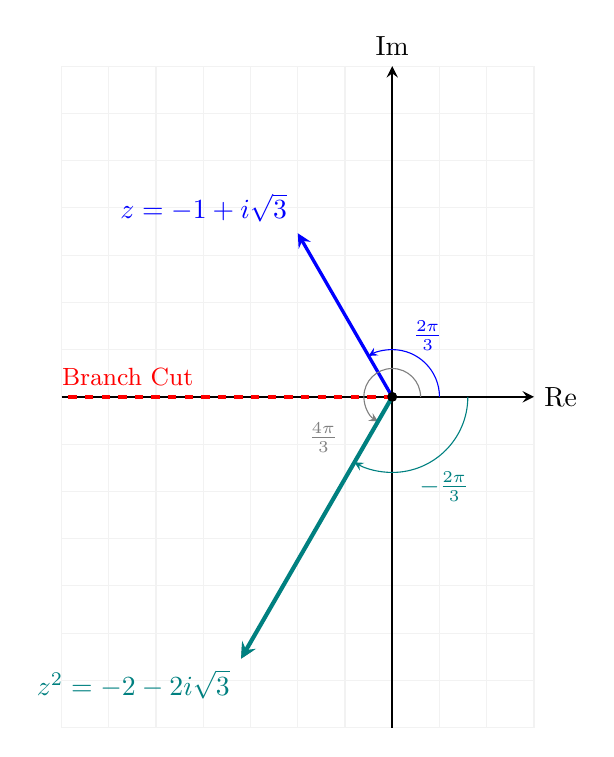
\begin{tikzpicture}[scale=1.2, >=stealth]
    % Grid lines
    \draw[color=gray!10, thin, step=0.5] (-3.5,-3.5) grid (1.5,3.5);
    
    % Axes
    \draw[->, thick] (-3.5,0) -- (1.5,0) node[right] {$\text{Re}$};
    \draw[->, thick] (0,-3.5) -- (0,3.5) node[above] {$\text{Im}$};
    
    % Branch cut
    \draw[line width=1.5pt, red, dashed] (0,0) -- (-3.5,0) node[pos=0.8, above, text=red] {\small Branch Cut};

    % Vector for z
    \draw[->, line width=1.2pt, blue] (0,0) -- (120:2) node[above left] {$z = -1+i\sqrt{3}$};
    \draw[->, blue, thin] (0.5,0) arc (0:120:0.5);
    \node[blue] at (60:0.75) {\small $\frac{2\pi}{3}$};

    % Vector for 2*Log(z) argument direction
    \draw[->, line width=1pt, gray, dashed] (0,0) -- (240:3.2);
    \draw[->, gray, thin] (0.3,0) arc (0:240:0.3);
    \node[gray, anchor=north east] at (200:0.5) {\small $\frac{4\pi}{3}$};

    % Vector for z^2 (Principal direction)
    \draw[->, line width=1.5pt, teal] (0,0) -- (-120:3.2) node[below left] {$z^2 = -2-2i\sqrt{3}$};
    \draw[->, teal, thin] (0.8,0) arc (0:-120:0.8);
    \node[teal] at (-60:1.1) {\small $-\frac{2\pi}{3}$};
    
    % Origin
    \fill[black] (0,0) circle (1.5pt);
\end{tikzpicture}
\end{center}

\end{tcolorbox}


\item Identify $|z-3i|+|z+3i|=8$ and $|z-1|=|z+i|$ geometrically.
\mk{15} \yr{MATH 245 | L-2/T-1 | 2021--22}

\item Let $R$ be the region in the $z$-plane bounded by $x=0$, $y=0$, $x=2$, $y=1$. Determine the region $R'$ of the $w$-plane into which $R$ is mapped under $w=\sqrt{2}\,e^{i\pi/4}z+(1-2i)$.
\mk{15} \yr{MATH 245 | L-2/T-1 | 2019--20}

\begin{tcolorbox}[enhanced,breakable,ansbox,colback=cE!4,colframe=cE,boxrule=0.8pt,arc=5pt,title={\textbf{Answer}},fonttitle=\bfseries\color{white},colbacktitle=cE]

To determine the region $R'$ in the $w$-plane, we analyze the components of the given linear transformation:
\[
w = \sqrt{2}\,e^{i\pi/4}z + (1-2i)
\]

\subsection*{1. Geometric Interpretation of the Transformation}

A linear complex transformation of the form $w = az + b$ can be broken down into three geometric operations:
\begin{enumerate}
    \item \textbf{Rotation:} The factor $e^{i\pi/4}$ rotates the region counterclockwise about the origin by an angle of $\theta = \frac{\pi}{4}$ ($45^\circ$).
    \item \textbf{Magnification (Scaling):} The scaling factor $|a| = \sqrt{2}$ stretches the region from the origin by a factor of $\sqrt{2}$.
    \item \textbf{Translation:} The term $b = 1 - 2i$ shifts the entire region by $1$ unit to the right and $2$ units down.
\end{enumerate}

We can simplify the transformation coefficient $a$ using Euler's formula:
\[
\sqrt{2}\,e^{i\pi/4} = \sqrt{2}\left(\cos\frac{\pi}{4} + i\sin\frac{\pi}{4}\right) = \sqrt{2}\left(\frac{1}{\sqrt{2}} + i\frac{1}{\sqrt{2}}\right) = 1 + i
\]

Substituting this back into the mapping equation gives:
\begin{equation}
w = (1+i)z + (1-2i)
\end{equation}

---

\subsection*{2. Mapping the Vertices of Region $R$}

The original region $R$ in the $z$-plane is a rectangle bounded by $x=0$, $y=0$, $x=2$, and $y=1$. The four vertices of this rectangle are:
\[
A = 0, \quad B = 2, \quad C = 2+i, \quad D = i
\]

Let us find their corresponding images $A', B', C', D'$ in the $w$-plane using Equation (1):

\begin{align*}
    A' = w(0)   &= (1+i)(0) + 1 - 2i = \boxed{1 - 2i} \\[0.5em]
    B' = w(2)   &= (1+i)(2) + 1 - 2i = 2 + 2i + 1 - 2i = \boxed{3} \\[0.5em]
    C' = w(2+i) &= (1+i)(2+i) + 1 - 2i = (2 + i + 2i - 1) + 1 - 2i = \boxed{2 + i} \\[0.5em]
    D' = w(i)   &= (1+i)(i) + 1 - 2i = (-1 + i) + 1 - 2i = \boxed{-i}
\end{align*}

---

\subsection*{3. Boundaries of the Mapped Region $R'$}

Let $w = u + iv$, where $u, v \in \mathbb{R}$. We can determine the boundary lines of the region $R'$ by finding the equations of the lines connecting the transformed vertices:

\begin{itemize}
    \item \textbf{Line $A'B'$ (connecting $(1,-2)$ and $(3,0)$):} 
          The slope is $\frac{0 - (-2)}{3 - 1} = 1$. The equation is $v - 0 = 1(u - 3) \implies \boxed{u - v = 3}$.
    \item \textbf{Line $B'C'$ (connecting $(3,0)$ and $(2,1)$):} 
          The slope is $\frac{1 - 0}{2 - 3} = -1$. The equation is $v - 0 = -1(u - 3) \implies \boxed{u + v = 3}$.
    \item \textbf{Line $C'D'$ (connecting $(2,1)$ and $(0,-1)$):} 
          The slope is $\frac{-1 - 1}{0 - 2} = 1$. The equation is $v - (-1) = 1(u - 0) \implies \boxed{u - v = 1}$.
    \item \textbf{Line $D'A'$ (connecting $(0,-1)$ and $(1,-2)$):} 
          The slope is $\frac{-2 - (-1)}{1 - 0} = -1$. The equation is $v - (-1) = -1(u - 0) \implies \boxed{u + v = -1}$.
    \item \textbf{Orientation:} Because orientation is preserved under a linear conformal mapping, the interior of the rectangle maps to the interior of the new boundaries.
\end{itemize}

Thus, the region $R'$ in the $w$-plane is a rectangle bounded by the lines:
\[
\boxed{1 \le u - v \le 3 \quad \text{and} \quad -1 \le u + v \le 3}
\]

---

\subsection*{4. Graphical Representation}

\begin{center}
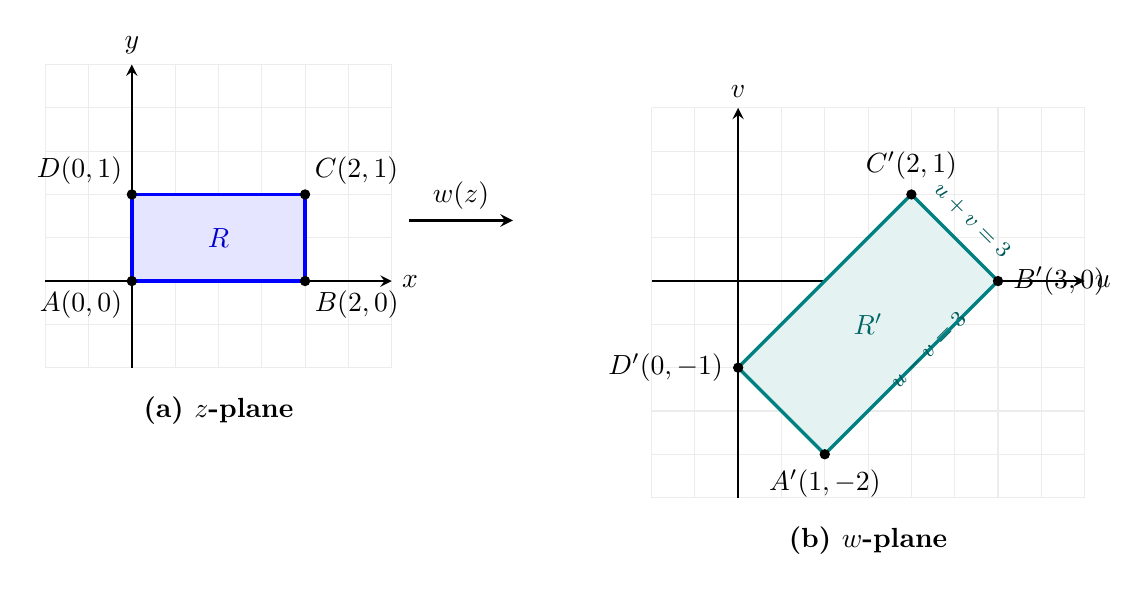
\begin{tikzpicture}[scale=1.1, >=stealth]

    % ================= z-plane =================
    \begin{scope}[xshift=-3.5cm]
        % Grid
        \draw[color=gray!15, thin, step=0.5] (-1,-1) grid (3,2.5);
        
        % Axes
        \draw[->, thick] (-1,0) -- (3,0) node[right] {$x$};
        \draw[->, thick] (0,-1) -- (0,2.5) node[above] {$y$};
        
        % Region R Shading & Outline
        \fill[blue!10] (0,0) rectangle (2,1);
        \draw[very thick, blue] (0,0) rectangle (2,1);
        
        % Vertices
        \filldraw[black] (0,0) circle (1.5pt) node[below left] {$A(0,0)$};
        \filldraw[black] (2,0) circle (1.5pt) node[below right] {$B(2,0)$};
        \filldraw[black] (2,1) circle (1.5pt) node[above right] {$C(2,1)$};
        \filldraw[black] (0,1) circle (1.5pt) node[above left] {$D(0,1)$};
        
        \node[blue!80!black] at (1,0.5) {$R$};
        \node at (1,-1.5) {\textbf{(a) $z$-plane}};
    \end{scope}

    % ================= Mapping Arrow =================
    \draw[->, line width=1pt] (-0.3,0.7) -- (0.9,0.7) node[midway, above] {$w(z)$};

    % ================= w-plane =================
    \begin{scope}[xshift=3.5cm]
        % Grid
        \draw[color=gray!15, thin, step=0.5] (-1,-2.5) grid (4,2);
        
        % Axes
        \draw[->, thick] (-1,0) -- (4,0) node[right] {$u$};
        \draw[->, thick] (0,-2.5) -- (0,2) node[above] {$v$};
        
        % Region R' Shading & Outline
        \fill[teal!10] (1,-2) -- (3,0) -- (2,1) -- (0,-1) -- cycle;
        \draw[very thick, teal] (1,-2) -- (3,0) -- (2,1) -- (0,-1) -- cycle;
        
        % Vertices
        \filldraw[black] (1,-2) circle (1.5pt) node[below, yshift=-2pt] {$A'(1,-2)$};
        \filldraw[black] (3,0) circle (1.5pt) node[right, xshift=2pt] {$B'(3,0)$};
        \filldraw[black] (2,1) circle (1.5pt) node[above, yshift=2pt] {$C'(2,1)$};
        \filldraw[black] (0,-1) circle (1.5pt) node[left, xshift=-2pt] {$D'(0,-1)$};
        
        % Boundary labels
        \node[teal!70!black, font=\footnotesize, rotate=45] at (2.2,-0.8) {$u-v=3$};
        \node[teal!70!black, font=\footnotesize, rotate=-45] at (2.7,0.7) {$u+v=3$};
        
        \node[teal!80!black] at (1.5,-0.5) {$R'$};
        \node at (1.5,-3) {\textbf{(b) $w$-plane}};
    \end{scope}

\end{tikzpicture}
\end{center}

\end{tcolorbox}

\item If $|z_{1}|=|z_{2}|$ and $\arg(z_{1})+\arg(z_{2})=0$, show that $z_{1}$ and $z_{2}$ are complex conjugates.
\mk{10} \yr{MATH 245 | L-2/T-1 | 2018--19}

\begin{tcolorbox}[enhanced,breakable,ansbox,colback=cE!4,colframe=cE,boxrule=0.8pt,arc=5pt,title={\textbf{Answer}},fonttitle=\bfseries\color{white},colbacktitle=cE]

To prove that $z_1$ and $z_2$ are complex conjugates, we can represent the complex numbers in their polar forms. 

Let the polar representations of $z_1$ and $z_2$ be:
\begin{align*}
    z_1 &= r_1 e^{i\theta_1} = r_1(\cos\theta_1 + i\sin\theta_1) \\
    z_2 &= r_2 e^{i\theta_2} = r_2(\cos\theta_2 + i\sin\theta_2)
\end{align*}
where $r_1 = |z_1|$, $r_2 = |z_2|$ are their magnitudes, and $\theta_1 = \arg(z_1)$, $\theta_2 = \arg(z_2)$ are their arguments.

\subsection*{1. Applying the Given Conditions}

We are given two specific conditions:
\begin{enumerate}
    \item \textbf{Equal Magnitudes:} 
    \[ |z_1| = |z_2| \implies r_1 = r_2 = r \]
    \item \textbf{Sum of Arguments is Zero:} 
    \[ \arg(z_1) + \arg(z_2) = 0 \implies \theta_1 + \theta_2 = 0 \implies \theta_2 = -\theta_1 \]
\end{enumerate}

\subsection*{2. Substituting into the Expression for $z_2$}

Now, substitute $r_2 = r$ and $\theta_2 = -\theta_1$ into the polar form of $z_2$:
\[
z_2 = r e^{i(-\theta_1)} = r \left[ \cos(-\theta_1) + i\sin(-\theta_1) \right]
\]

Using the trigonometric identities for negative angles, $\cos(-\theta) = \cos\theta$ and $\sin(-\theta) = -\sin\theta$:
\begin{equation}
z_2 = r (\cos\theta_1 - i\sin\theta_1)
\end{equation}

\subsection*{3. Comparing with the Complex Conjugate of $z_1$}

By definition, the complex conjugate of $z_1$ (denoted as $\overline{z_1}$) is found by changing the sign of its imaginary part:
\begin{equation}
\overline{z_1} = \overline{r(\cos\theta_1 + i\sin\theta_1)} = r(\cos\theta_1 - i\sin\theta_1)
\end{equation}

Comparing Equation (1) and Equation (2), we clearly see that:
\[
\boxed{z_2 = \overline{z_1}}
\]

Thus, $z_1$ and $z_2$ are complex conjugates of each other. $\blacksquare$

\subsection*{Geometrical Visualization}

Geometrically, a complex conjugate represents a reflection across the real axis ($\text{Re}(z)$). Because $z_1$ and $z_2$ share the same distance $r$ from the origin and have equal but opposite angles relative to the real axis, they form a perfect mirror image across the horizontal line.

\begin{center}
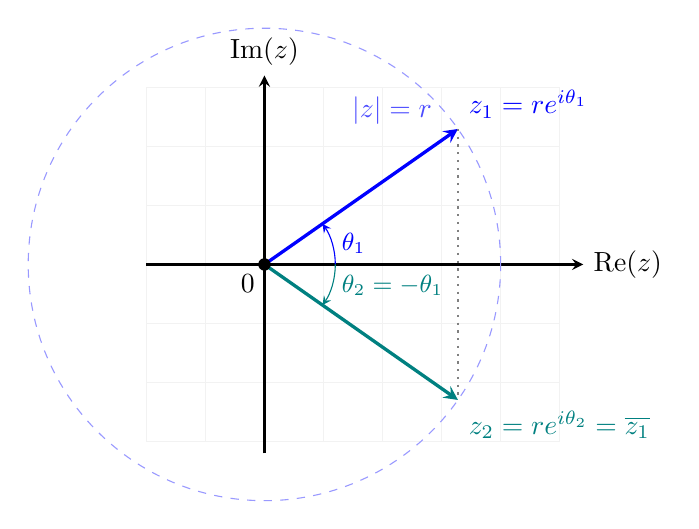
\begin{tikzpicture}[scale=1.5, >=stealth]
    % Grid lines
    \draw[color=gray!10, thin, step=0.5] (-1,-1.5) grid (2.5,1.5);
    
    % Axes
    \draw[->, thick] (-1,0) -- (2.7,0) node[right] {$\text{Re}(z)$};
    \draw[->, thick] (0,-1.6) -- (0,1.6) node[above] {$\text{Im}(z)$};
    
    % Dashed circle segment indicating equal radii
    \draw[dashed, blue!40] (0,0) circle (2);
    \node[blue!70, anchor=north east] at (1.5,1.5) {$|z|=r$};
    
    % Vector for z1
    \draw[->, line width=1.2pt, blue] (0,0) -- (35:2) node[above right] {$z_1 = re^{i\theta_1}$};
    \draw[->, blue, thin] (0.6,0) arc (0:35:0.6);
    \node[blue, anchor=west] at (17:0.6) {\small $\theta_1$};
    
    % Vector for z2
    \draw[->, line width=1.2pt, teal] (0,0) -- (-35:2) node[below right] {$z_2 = re^{i\theta_2} = \overline{z_1}$};
    \draw[->, teal, thin] (0.6,0) arc (0:-35:0.6);
    \node[teal, anchor=west] at (-17:0.6) {\small $\theta_2 = -\theta_1$};
    
    % Vertical reflection helper line
    \draw[dotted, gray, thick] (35:2) -- (-35:2);
    
    % Origin
    \fill[black] (0,0) circle (1.5pt) node[below left] {$0$};
\end{tikzpicture}
\end{center}

\end{tcolorbox}

\item Prove that if the ratio $\dfrac{z-i}{z-1}$ is purely imaginary, then the point $z$ lies on the circle whose centre is $\tfrac{1}{2}(1+i)$ and radius $\dfrac{1}{\sqrt{2}}$.
\mk{10} \yr{MATH 245 | L-2/T-1 | 2018--19}

\begin{tcolorbox}[enhanced,breakable,ansbox,colback=cE!4,colframe=cE,boxrule=0.8pt,arc=5pt,title={\textbf{Answer}},fonttitle=\bfseries\color{white},colbacktitle=cE]

To prove that the point $z = x + iy$ lies on the specified circle, we analyze the condition that the complex expression
\[
w = \frac{z-i}{z-1}
\]
is purely imaginary. A complex number $w$ is purely imaginary if and only if its real part is zero ($\text{Re}(w) = 0$), given that $z \neq 1$.

\subsection*{1. Algebraic Proof}

Let $z = x + iy$, where $x, y \in \mathbb{R}$. Substituting this into the given expression yields:
\[
w = \frac{(x + iy) - i}{(x + iy) - 1} = \frac{x + i(y-1)}{(x-1) + iy}
\]

To separate $w$ into its real and imaginary parts, we realize the denominator by multiplying the numerator and denominator by the complex conjugate of the denominator, which is $(x-1) - iy$:
\begin{align*}
w &= \frac{[x + i(y-1)][(x-1) - iy]}{[(x-1) + iy][(x-1) - iy]} \\[0.8em]
&= \frac{x(x-1) - ixy + i(y-1)(x-1) - i^2y(y-1)}{(x-1)^2 + y^2} \\[0.8em]
&= \frac{[x(x-1) + y(y-1)] + i[(y-1)(x-1) - xy]}{(x-1)^2 + y^2}
\end{align*}

Extracting the real part of $w$, we get:
\[
\text{Re}(w) = \frac{x(x-1) + y(y-1)}{(x-1)^2 + y^2}
\]

Since $w$ is given to be purely imaginary, we set $\text{Re}(w) = 0$:
\[
\frac{x(x-1) + y(y-1)}{(x-1)^2 + y^2} = 0
\]
Assuming $z \neq 1$ (so the denominator is non-zero), this implies:
\begin{align*}
x(x-1) + y(y-1) &= 0 \\
x^2 - x + y^2 - y &= 0
\end{align*}

We now complete the square for both the $x$ and $y$ terms:
\begin{align*}
\left(x^2 - x + \frac{1}{4}\right) + \left(y^2 - y + \frac{1}{4}\right) &= 0 + \frac{1}{4} + \frac{1}{4} \\[0.5em]
\left(x - \frac{1}{2}\right)^2 + \left(y - \frac{1}{2}\right)^2 &= \frac{1}{2}
\end{align*}

The standard equation of a circle in the Cartesian plane is $(x-x_0)^2 + (y-y_0)^2 = R^2$. Matching terms shows that this equation represents a circle with:
\begin{align*}
\text{Centre } (x_0, y_0) &= \left(\frac{1}{2}, \frac{1}{2}\right) \implies \boxed{z_0 = \frac{1}{2}(1+i)} \\[0.5em]
\text{Radius } R &= \sqrt{\frac{1}{2}} = \boxed{\frac{1}{\sqrt{2}}}
\end{align*}
Thus, the point $z$ lies on the designated circle (excluding the point $z=1$ where the ratio is undefined). $\blacksquare$

---

\subsection*{2. Alternative Geometric Proof}

The expression can also be interpreted geometrically using arguments. The condition that $\frac{z-i}{z-1}$ is purely imaginary means that its argument must be $\pm \frac{\pi}{2}$:
\[
\arg\left(\frac{z-i}{z-1}\right) = \arg(z-i) - \arg(z-1) = \pm \frac{\pi}{2}
\]
This states that the vector from $1$ to $z$ and the vector from $i$ to $z$ are perpendicular to each other. By Thales's Theorem, the locus of a point $z$ that forms a right angle with two fixed points $A(i)$ and $B(1)$ is a circle having the line segment $AB$ as its diameter.

\begin{itemize}
    \item \textbf{Centre:} The midpoint of the diameter connecting $1$ and $i$:
    \[ z_0 = \frac{1 + i}{2} = \frac{1}{2}(1+i) \]
    \item \textbf{Radius:} Half the distance between $1$ and $i$:
    \[ R = \frac{1}{2}|i - 1| = \frac{1}{2}\sqrt{(-1)^2 + 1^2} = \frac{\sqrt{2}}{2} = \frac{1}{\sqrt{2}} \].
\end{itemize}

---

\subsection*{3. Geometrical Visualization}



\begin{center}
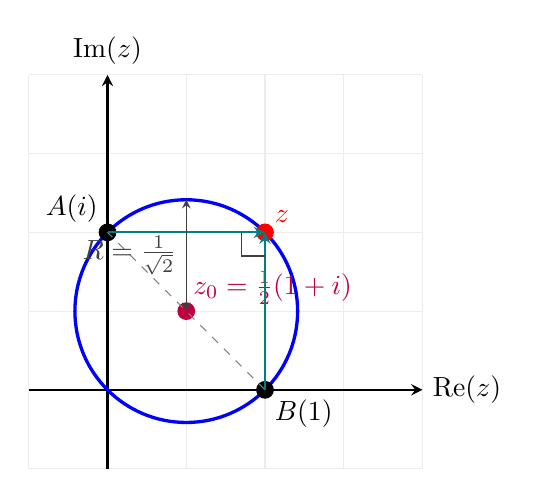
\begin{tikzpicture}[scale=2.0, >=stealth]
    % Grid lines
    \draw[color=gray!15, thin, step=0.5] (-0.5,-0.5) grid (2.0,2.0);
    
    % Axes
    \draw[->, thick] (-0.5,0) -- (2.0,0) node[right] {$\text{Re}(z)$};
    \draw[->, thick] (0,-0.5) -- (0,2.0) node[above] {$\text{Im}(z)$};
    
    % Center and Circle Parameters
    % Center = (0.5, 0.5), Radius = 1/sqrt(2) approx 0.7071
    \coordinate (O) at (0.5,0.5);
    \draw[very thick, blue] (O) circle (0.7071);
    
    % Core points
    \filldraw[black] (1,0) circle (1.5pt) node[below right] {$B(1)$};
    \filldraw[black] (0,1) circle (1.5pt) node[above left] {$A(i)$};
    \filldraw[purple] (O) circle (1.5pt) node[anchor=south west, xshift=-1pt, yshift=-1pt] {$z_0 = \frac{1}{2}(1+i)$};
    
    % Diameter line
    \draw[dashed, gray] (1,0) -- (0,1);
    
    % Random point z on the circle to demonstrate right angle
    % Choose angle 45 degrees from center -> (0.5 + 0.5, 0.5 + 0.5) = (1,1)
    \coordinate (Z) at (1,1);
    \filldraw[red] (Z) circle (1.5pt) node[above right] {$z$};
    
    % Vectors forming the right angle
    \draw[->, thick, teal] (1,0) -- (Z);
    \draw[->, thick, teal] (0,1) -- (Z);
    
    % Right angle symbol indication
    \path (Z) -- (1,0) coordinate[pos=0.15] (p1);
    \path (Z) -- (0,1) coordinate[pos=0.15] (p2);
    \coordinate (p3) at ($(p1)+(p2)-(Z)$);
    \draw[thin, darkgray] (p1) -- (p3) -- (p2);
    
    % Radius Label
    \draw[<->, darkgray, thin] (O) -- (0.5, 1.2071) node[midway, left] {$R = \frac{1}{\sqrt{2}}$};
\end{tikzpicture}
\end{center}

\end{tcolorbox}

\item Find all roots of $(-2\sqrt{3}-2i)^{1/4}$ in rectangular coordinates and exhibit them graphically.
\mk{13} \yr{MATH 241 | L-2/T-1 | 2015--16}

\begin{tcolorbox}[enhanced,breakable,ansbox,colback=cE!4,colframe=cE,boxrule=0.8pt,arc=5pt,title={\textbf{Answer}},fonttitle=\bfseries\color{white},colbacktitle=cE]

To find all the roots of $z^{1/4}$ where $z = -2\sqrt{3} - 2i$, we will first convert $z$ to its polar form, use De Moivre's formula to find the roots, and then convert them back to exact rectangular coordinates.

\subsection*{1. Polar Form of $z$}
Given $z = x + iy = -2\sqrt{3} - 2i$, we find its magnitude $r$ and principal argument $\theta$:
\[
r = |z| = \sqrt{(-2\sqrt{3})^2 + (-2)^2} = \sqrt{12 + 4} = 4
\]
Since both the real and imaginary parts are negative, $z$ lies in the third quadrant. The reference angle $\alpha$ is:
\[
\alpha = \tan^{-1}\left(\left|\frac{-2}{-2\sqrt{3}}\right|\right) = \tan^{-1}\left(\frac{1}{\sqrt{3}}\right) = \frac{\pi}{6} = 30^\circ
\]
Thus, the argument measured counterclockwise from the positive real axis is:
\[
\theta = \pi + \frac{\pi}{6} = \frac{7\pi}{6} \quad (210^\circ)
\]
The polar form of $z$ is:
\[
z = 4 \exp\left(i \frac{7\pi}{6}\right)
\]

\subsection*{2. Finding the Fourth Roots}
Using De Moivre's formula, the four roots $w_k = z^{1/4}$ are given by:
\[
w_k = 4^{1/4} \exp\left( i \frac{\frac{7\pi}{6} + 2k\pi}{4} \right) = \sqrt{2} \exp\left( i \left( \frac{7\pi}{24} + \frac{k\pi}{2} \right) \right) \quad \text{for } k = 0, 1, 2, 3
\]
The magnitude for all roots is $R = \sqrt{2}$. The angles are:
\begin{align*}
    k = 0 &: \quad \theta_0 = \frac{7\pi}{24} = 52.5^\circ \\
    k = 1 &: \quad \theta_1 = \frac{7\pi}{24} + \frac{\pi}{2} = 142.5^\circ \\
    k = 2 &: \quad \theta_2 = \frac{7\pi}{24} + \pi = 232.5^\circ \\
    k = 3 &: \quad \theta_3 = \frac{7\pi}{24} + \frac{3\pi}{2} = 322.5^\circ
\end{align*}

\subsection*{3. Exact Rectangular Coordinates}
To express the first root $w_0$ in rectangular form ($w_0 = A + iB$), we need to evaluate $\sqrt{2}\cos(52.5^\circ)$ and $\sqrt{2}\sin(52.5^\circ)$. We use the half-angle formulas $\cos(\theta/2) = \sqrt{\frac{1+\cos\theta}{2}}$ and $\sin(\theta/2) = \sqrt{\frac{1-\cos\theta}{2}}$. 

First, note that $105^\circ = 60^\circ + 45^\circ$, giving:
\[
\cos(105^\circ) = \cos(60^\circ)\cos(45^\circ) - \sin(60^\circ)\sin(45^\circ) = \frac{\sqrt{2}-\sqrt{6}}{4}
\]
Now we find the real part $A = \sqrt{2}\cos(52.5^\circ)$:
\[
A = \sqrt{2} \sqrt{\frac{1 + \frac{\sqrt{2}-\sqrt{6}}{4}}{2}} = \sqrt{2} \sqrt{\frac{4+\sqrt{2}-\sqrt{6}}{8}} = \frac{1}{2}\sqrt{4+\sqrt{2}-\sqrt{6}} \approx 0.861
\]
Similarly, the imaginary part $B = \sqrt{2}\sin(52.5^\circ)$:
\[
B = \sqrt{2} \sqrt{\frac{1 - \frac{\sqrt{2}-\sqrt{6}}{4}}{2}} = \sqrt{2} \sqrt{\frac{4-\sqrt{2}+\sqrt{6}}{8}} = \frac{1}{2}\sqrt{4-\sqrt{2}+\sqrt{6}} \approx 1.122
\]

Since adding $\frac{\pi}{2}$ ($90^\circ$) simply multiplies a complex number by $i$, transforming $(x+iy) \to (-y+ix)$, the four roots in exact rectangular coordinates are:
\begin{align*}
    w_0 &= \phantom{-}A + iB \approx \phantom{-}0.861 + 1.122i \\
    w_1 = w_0 \cdot i &= -B + iA \approx -1.122 + 0.861i \\
    w_2 = w_1 \cdot i &= -A - iB \approx -0.861 - 1.122i \\
    w_3 = w_2 \cdot i &= \phantom{-}B - iA \approx \phantom{-}1.122 - 0.861i
\end{align*}

\begin{equation}
\boxed{w_k \in \left\{ \pm (A + iB), \pm (-B + iA) \right\} \quad \text{where } A = \tfrac{1}{2}\sqrt{4+\sqrt{2}-\sqrt{6}}, \; B = \tfrac{1}{2}\sqrt{4-\sqrt{2}+\sqrt{6}} }
\end{equation}

\subsection*{4. Graphical Representation}

The roots lie symmetrically on a circle of radius $\sqrt{2}$ centered at the origin, forming the vertices of a square.

\begin{center}
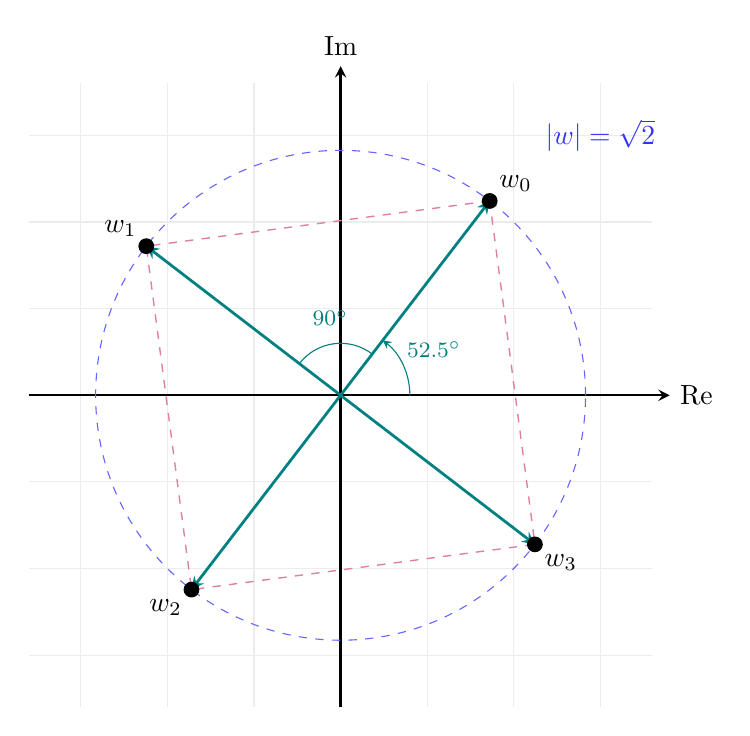
\begin{tikzpicture}[scale=2.2, >=stealth]
    % Grid lines
    \draw[color=gray!15, thin, step=0.5] (-1.8,-1.8) grid (1.8,1.8);
    
    % Axes
    \draw[->, thick] (-1.8,0) -- (1.9,0) node[right] {$\text{Re}$};
    \draw[->, thick] (0,-1.8) -- (0,1.9) node[above] {$\text{Im}$};
    
    % Circle of radius sqrt(2) approx 1.414
    \draw[dashed, blue!60, thin] (0,0) circle (1.414);
    
    % Square connecting the roots
    \draw[line width=0.5pt, draw=purple!50, dashed] (52.5:1.414) -- (142.5:1.414) -- (232.5:1.414) -- (322.5:1.414) -- cycle;
    
    % Root vectors and points
    % w0
    \draw[->, line width=1pt, teal] (0,0) -- (52.5:1.414);
    \filldraw[black] (52.5:1.414) circle (1.2pt) node[anchor=south west] {$w_0$};
    \draw[->, teal, thin] (0.4,0) arc (0:52.5:0.4);
    \node[teal] at (26:0.6) {\footnotesize $52.5^\circ$};

    % w1
    \draw[->, line width=1pt, teal] (0,0) -- (142.5:1.414);
    \filldraw[black] (142.5:1.414) circle (1.2pt) node[anchor=south east] {$w_1$};
    
    % Right angle indication between w0 and w1
    \draw[teal, thin] (52.5:0.3) arc (52.5:142.5:0.3);
    \node[teal] at (97.5:0.45) {\footnotesize $90^\circ$};

    % w2
    \draw[->, line width=1pt, teal] (0,0) -- (232.5:1.414);
    \filldraw[black] (232.5:1.414) circle (1.2pt) node[anchor=north east] {$w_2$};

    % w3
    \draw[->, line width=1pt, teal] (0,0) -- (322.5:1.414);
    \filldraw[black] (322.5:1.414) circle (1.2pt) node[anchor=north west] {$w_3$};
    
    % Label the circle
    \node[blue!80] at (1.5,1.5) {$|w| = \sqrt{2}$};
\end{tikzpicture}
\end{center}

\end{tcolorbox}

\item Describe mathematically and graphically the region represented by $z(\bar{z}+2)=3$.
\mk{10} \yr{MATH 241 | L-2/T-1 | 2015--16}

\begin{tcolorbox}[enhanced,breakable,ansbox,colback=cE!4,colframe=cE,boxrule=0.8pt,arc=5pt,title={\textbf{Answer}},fonttitle=\bfseries\color{white},colbacktitle=cE]

To mathematically and graphically describe the region represented by the equation $z(\bar{z}+2)=3$, we will express the complex number $z$ in its rectangular form, $z = x + iy$, where $x$ and $y$ are real numbers.

\subsection*{1. Mathematical Description}

First, recall that the complex conjugate of $z$ is $\bar{z} = x - iy$, and the product of a complex number and its conjugate is $z\bar{z} = |z|^2 = x^2 + y^2$. 

Substitute $z$ and $\bar{z}$ into the given equation:
\begin{align*}
    z(\bar{z} + 2) &= 3 \\
    z\bar{z} + 2z &= 3 \\
    (x^2 + y^2) + 2(x + iy) &= 3 \\
    (x^2 + y^2 + 2x) + i(2y) &= 3 + i(0)
\end{align*}

For two complex numbers to be equal, their real and imaginary parts must be equal. This gives us a system of two equations:
\begin{align}
    \text{Real part:} \quad & x^2 + y^2 + 2x = 3 \\
    \text{Imaginary part:} \quad & 2y = 0 
\end{align}

From Equation (2), we immediately find that:
\[
y = 0
\]
This indicates that any solution must lie strictly on the real axis. Now, substitute $y = 0$ into Equation (1):
\begin{align*}
    x^2 + 0^2 + 2x &= 3 \\
    x^2 + 2x - 3 &= 0
\end{align*}

Factoring the quadratic equation yields:
\[
    (x + 3)(x - 1) = 0 \implies x = -3 \quad \text{or} \quad x = 1
\]

\textbf{Conclusion:} 
Although the term "region" often implies an area or a continuous curve (like a circle or a line), the requirement that the imaginary part is zero restricts the solution. The "region" represented by this equation consists entirely of \textbf{two discrete points} on the real axis: $z = 1$ and $z = -3$. 

\textit{Note: If the equation had instead been $z\bar{z} + z + \bar{z} = 3$ (which guarantees a purely real left-hand side), it would represent a circle. However, the exact equation $z(\bar{z}+2)=3$ collapses to just two points.}

\subsection*{2. Graphical Representation}

Graphically, this is represented by plotting the two exact coordinates $(-3, 0)$ and $(1, 0)$ in the complex plane.

\begin{center}
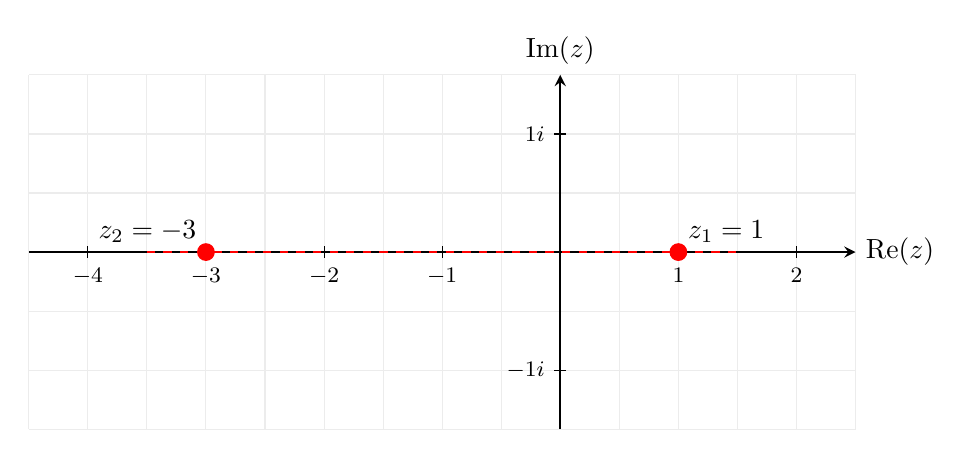
\begin{tikzpicture}[scale=1.5, >=stealth]
    % Grid lines
    \draw[color=gray!15, thin, step=0.5] (-4.5,-1.5) grid (2.5,1.5);
    
    % Axes
    \draw[->, thick] (-4.5,0) -- (2.5,0) node[right] {$\text{Re}(z)$};
    \draw[->, thick] (0,-1.5) -- (0,1.5) node[above] {$\text{Im}(z)$};
    
    % Tick marks for context
    \foreach \x in {-4,-3,-2,-1,1,2} {
        \draw (\x, 0.05) -- (\x, -0.05) node[below] {\footnotesize $\x$};
    }
    \foreach \y in {-1,1} {
        \draw (0.05, \y) -- (-0.05, \y) node[left] {\footnotesize $\y i$};
    }
    
    % The two solution points
    \filldraw[red] (1,0) circle (2pt) node[above right, text=black] {$z_1 = 1$};
    \filldraw[red] (-3,0) circle (2pt) node[above left, text=black] {$z_2 = -3$};
    
    % Highlight that they are on the real axis
    \draw[red, thick, dashed] (-3.5,0) -- (1.5,0);

\end{tikzpicture}
\end{center}

\end{tcolorbox}

\item Find the image of $\operatorname{Re}(z)\ge 0$ under the transformation $w=\dfrac{z-1}{z+1}$. Sketch the region $\operatorname{Re}(z)\ge 0$ and its image.
\mk{12} \yr{MATH 241 | L-2/T-1 | 2015--16}

\begin{tcolorbox}[enhanced,breakable,ansbox,colback=cE!4,colframe=cE,boxrule=0.8pt,arc=5pt,title={\textbf{Answer}},fonttitle=\bfseries\color{white},colbacktitle=cE]

To find the image of the region $\operatorname{Re}(z) \ge 0$ under the given bilinear (Möbius) transformation, we will express $z$ in terms of $w$ and apply the given inequality.

\subsection*{1. Inverse Transformation}
Given the transformation:
\[
w = \frac{z-1}{z+1}
\]
We solve for $z$ in terms of $w$:
\begin{align*}
w(z+1) &= z-1 \\
wz + w &= z - 1 \\
wz - z &= -w - 1 \\
z(w - 1) &= -(w + 1) \\
z &= \frac{1+w}{1-w}
\end{align*}

\subsection*{2. Applying the Region Condition}
We are given the region $\operatorname{Re}(z) \ge 0$. Using the inverse transformation, we can write:
\[
\operatorname{Re}(z) = \operatorname{Re}\left( \frac{1+w}{1-w} \right) \ge 0
\]
To find the real part of $\frac{1+w}{1-w}$, we multiply the numerator and the denominator by the complex conjugate of the denominator, which is $1-\bar{w}$:
\begin{align*}
\frac{1+w}{1-w} \cdot \frac{1-\bar{w}}{1-\bar{w}} &= \frac{(1+w)(1-\bar{w})}{|1-w|^2} \\
&= \frac{1 - \bar{w} + w - w\bar{w}}{|1-w|^2}
\end{align*}
Recall that $w\bar{w} = |w|^2$ and $w - \bar{w} = 2i\operatorname{Im}(w)$. Substituting these in gives:
\[
\frac{1 - |w|^2 + 2i\operatorname{Im}(w)}{|1-w|^2}
\]
The real part of this expression is:
\[
\operatorname{Re}(z) = \frac{1 - |w|^2}{|1-w|^2}
\]

Since we require $\operatorname{Re}(z) \ge 0$, and knowing that the denominator $|1-w|^2$ is always strictly positive (for $w \neq 1$), the numerator must be non-negative:
\begin{align*}
1 - |w|^2 &\ge 0 \\
|w|^2 &\le 1 \\
|w| &\le 1
\end{align*}

\textbf{Conclusion:} 
The right half-plane $\operatorname{Re}(z) \ge 0$ is mapped to the closed unit disk $|w| \le 1$ in the $w$-plane. The boundary (the imaginary axis in the $z$-plane) maps to the boundary of the unit circle ($|w|=1$).

---

\subsection*{3. Graphical Representation}

The sketches below illustrate the right half-plane in the $z$-plane mapping to the interior and boundary of the unit circle in the $w$-plane.

\begin{center}
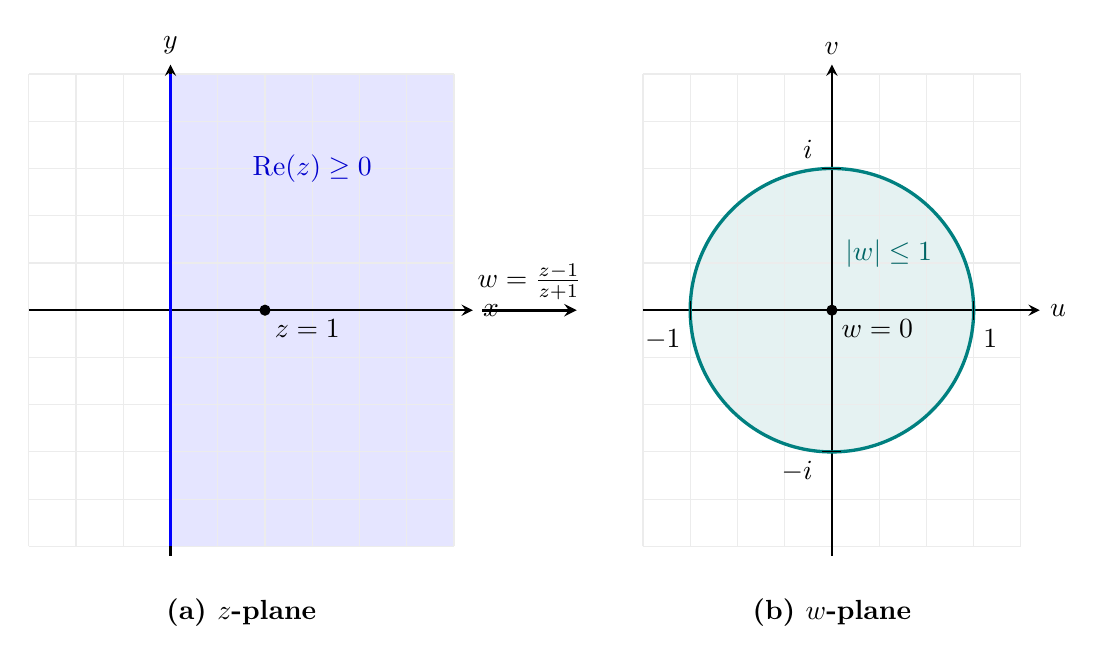
\begin{tikzpicture}[scale=1.2, >=stealth]

    % ================= z-plane =================
    \begin{scope}[xshift=-3.5cm]
        % Shading the region Re(z) >= 0
        \fill[blue!10] (0,-2.5) rectangle (3,2.5);
        
        % Grid
        \draw[color=gray!15, thin, step=0.5] (-1.5,-2.5) grid (3,2.5);
        
        % Axes
        \draw[->, thick] (-1.5,0) -- (3.2,0) node[right] {$x$};
        \draw[->, thick] (0,-2.6) -- (0,2.6) node[above] {$y$};
        
        % Boundary line (y-axis)
        \draw[very thick, blue] (0,-2.5) -- (0,2.5);
        
        % Labels
        \node[blue!80!black] at (1.5,1.5) {$\operatorname{Re}(z) \ge 0$};
        \node at (0.75,-3.2) {\textbf{(a) $z$-plane}};
        
        % Test point
        \filldraw[black] (1,0) circle (1.5pt) node[below right] {$z=1$};
    \end{scope}

    % ================= Mapping Arrow =================
    \draw[->, line width=1pt] (-0.2,0) -- (0.8,0) node[midway, above] {$w = \frac{z-1}{z+1}$};

    % ================= w-plane =================
    \begin{scope}[xshift=3.5cm]
        % Shading the region |w| <= 1
        \fill[teal!10] (0,0) circle (1.5);
        
        % Grid
        \draw[color=gray!15, thin, step=0.5] (-2,-2.5) grid (2,2.5);
        
        % Axes
        \draw[->, thick] (-2,0) -- (2.2,0) node[right] {$u$};
        \draw[->, thick] (0,-2.6) -- (0,2.6) node[above] {$v$};
        
        % Boundary circle |w| = 1
        \draw[very thick, teal] (0,0) circle (1.5);
        
        % Circle radius labels
        \draw (1.5, 0.1) -- (1.5, -0.1) node[below right] {$1$};
        \draw (-1.5, 0.1) -- (-1.5, -0.1) node[below left] {$-1$};
        \draw (0.1, 1.5) -- (-0.1, 1.5) node[above left] {$i$};
        \draw (0.1, -1.5) -- (-0.1, -1.5) node[below left] {$-i$};
        
        % Labels
        \node[teal!80!black] at (0.6,0.6) {$|w| \le 1$};
        \node at (0,-3.2) {\textbf{(b) $w$-plane}};
        
        % Image of test point
        \filldraw[black] (0,0) circle (1.5pt) node[below right] {$w=0$};
    \end{scope}

\end{tikzpicture}
\end{center}

\end{tcolorbox}

\item Prove that $|z_{1}+z_{2}| \ge \bigl||z_{1}|-|z_{2}|\bigr|$ where $z_{1},z_{2}$ are nonzero complex numbers.
\mk{8} \yr{MATH 241 | L-2/T-1 | 2014--15}

\begin{tcolorbox}[enhanced,breakable,ansbox,colback=cE!4,colframe=cE,boxrule=0.8pt,arc=5pt,title={\textbf{Answer}},fonttitle=\bfseries\color{white},colbacktitle=cE]

To prove the reverse triangle inequality $|z_{1}+z_{2}| \ge \bigl||z_{1}|-|z_{2}|\bigr|$, we can use the standard triangle inequality for complex numbers, which states that for any two complex numbers $a$ and $b$:
\[
|a + b| \le |a| + |b|
\]

\subsection*{1. Algebraic Proof}

\textbf{Step 1:} We can express $z_1$ in terms of $z_1 + z_2$ and $-z_2$:
\[
z_1 = (z_1 + z_2) - z_2
\]
Applying the standard triangle inequality where $a = z_1 + z_2$ and $b = -z_2$, we get:
\[
|z_1| = |(z_1 + z_2) - z_2| \le |z_1 + z_2| + |-z_2|
\]
Since the absolute value of a complex number and its negative are equal ($|-z_2| = |z_2|$), we have:
\[
|z_1| \le |z_1 + z_2| + |z_2|
\]
Subtracting $|z_2|$ from both sides yields our first key inequality:
\begin{equation}
|z_1| - |z_2| \le |z_1 + z_2|
\end{equation}

\textbf{Step 2:} Now, we apply the exact same logic but swap the roles of $z_1$ and $z_2$. We express $z_2$ as:
\[
z_2 = (z_1 + z_2) - z_1
\]
Applying the triangle inequality again:
\[
|z_2| = |(z_1 + z_2) - z_1| \le |z_1 + z_2| + |-z_1|
\]
\[
|z_2| \le |z_1 + z_2| + |z_1|
\]
Subtracting $|z_1|$ from both sides yields:
\[
|z_2| - |z_1| \le |z_1 + z_2|
\]
Multiplying the left side by $-1$ gives our second key inequality:
\begin{equation}
-(|z_1| - |z_2|) \le |z_1 + z_2|
\end{equation}

\textbf{Step 3:} We now have two statements from Equations (1) and (2):
\begin{align*}
    |z_1| - |z_2| &\le |z_1 + z_2| \\
    -(|z_1| - |z_2|) &\le |z_1 + z_2|
\end{align*}
Recall the fundamental property of real numbers: if a number $Y$ is greater than or equal to both $X$ and $-X$, then $Y$ must be greater than or equal to the absolute value of $X$ ($Y \ge |X|$). 

Let $X = |z_1| - |z_2|$ and $Y = |z_1 + z_2|$. This directly implies:
\[
\boxed{ \bigl||z_1| - |z_2|\bigr| \le |z_1 + z_2| }
\]
Thus, the statement is proven. $\blacksquare$

---

\subsection*{2. Geometric Interpretation}

In the complex plane, the points $0$, $z_1$, and $z_1+z_2$ form a triangle. The lengths of the sides of this triangle are:
\begin{itemize}
    \item Distance from $0$ to $z_1 = |z_1|$
    \item Distance from $z_1$ to $z_1+z_2 = |z_2|$ (since it is a parallel translation of the vector $z_2$)
    \item Distance from $0$ to $z_1+z_2 = |z_1+z_2|$
\end{itemize}

According to the fundamental geometric property of triangles, the length of any side of a triangle must be greater than or equal to the absolute difference of the lengths of the other two sides. Applying this to our side lengths directly yields $|z_1+z_2| \ge \bigl||z_1| - |z_2|\bigr|$.

\begin{center}
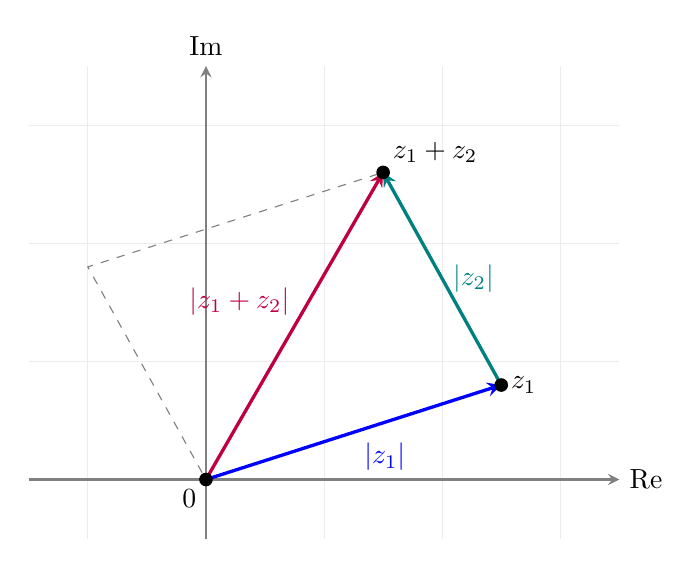
\begin{tikzpicture}[scale=1.5, >=stealth]
    % Grid lines (optional, kept light)
    \draw[color=gray!15, thin, step=1] (-1.5,-0.5) grid (3.5,3.5);
    
    % Axes
    \draw[->, thick, gray] (-1.5,0) -- (3.5,0) node[right, text=black] {$\text{Re}$};
    \draw[->, thick, gray] (0,-0.5) -- (0,3.5) node[above, text=black] {$\text{Im}$};

    % Coordinates for the vectors
    \coordinate (O) at (0,0);
    \coordinate (Z1) at (2.5, 0.8);
    \coordinate (Z2) at (-1, 1.8);
    \coordinate (Z1Z2) at (1.5, 2.6); % Z1 + Z2

    % Parallelogram (dashed) for context
    \draw[dashed, gray] (Z1) -- (Z1Z2) -- (Z2) -- (O);

    % Vectors forming the main triangle O -> Z1 -> Z1Z2
    \draw[->, line width=1.2pt, blue] (O) -- (Z1) node[midway, below right] {$|z_1|$};
    \draw[->, line width=1.2pt, teal] (Z1) -- (Z1Z2) node[midway, right] {$|z_2|$};
    
    % Resultant Vector
    \draw[->, line width=1.2pt, purple] (O) -- (Z1Z2) node[midway, above left, xshift=2pt] {$|z_1+z_2|$};

    % Points and Labels
    \filldraw[black] (O) circle (1.5pt) node[below left] {$0$};
    \filldraw[black] (Z1) circle (1.5pt) node[right] {$z_1$};
    \filldraw[black] (Z1Z2) circle (1.5pt) node[above right] {$z_1+z_2$};

\end{tikzpicture}
\end{center}

\end{tcolorbox}

\item Show that the equation $|z-z_{0}|=R$ represents a circle centred at $z_{0}$ with radius $R$, which can be written as $z\bar{z}-2\operatorname{Re}(z\bar{z}_{0})+|z_{0}|^{2}=R^{2}$.
\mk{7} \yr{MATH 241 | L-2/T-1 | 2014--15}

\begin{tcolorbox}[enhanced,breakable,ansbox,colback=cE!4,colframe=cE,boxrule=0.8pt,arc=5pt,title={\textbf{Answer}},fonttitle=\bfseries\color{white},colbacktitle=cE]

\subsection*{1. Geometric Interpretation}

In the complex plane, the absolute value (or modulus) $|w|$ of a complex number $w$ represents its distance from the origin. Therefore, the expression $|z - z_0|$ represents the geometric distance between the point $z$ and the fixed point $z_0$. 

The equation $|z - z_0| = R$ states that the distance between any point $z$ on the locus and the fixed point $z_0$ is always a constant value $R$ (where $R > 0$). By definition, the locus of points in a plane that are at a constant distance from a fixed point is a \textbf{circle}. 
\begin{itemize}
    \item The fixed point $z_0$ is the \textbf{centre} of the circle.
    \item The constant distance $R$ is the \textbf{radius}.
\end{itemize}

\subsection*{2. Algebraic Expansion}

To express this equation in the requested expanded form, we start by squaring both sides of the equation:
\[
|z - z_0|^2 = R^2
\]

We use the fundamental property of complex numbers that the square of the modulus of any complex number $w$ is equal to the product of $w$ and its complex conjugate $\bar{w}$ (i.e., $|w|^2 = w\bar{w}$). Applying this to $w = (z - z_0)$:
\begin{equation}
(z - z_0)\overline{(z - z_0)} = R^2
\end{equation}

Since the conjugate of a difference is the difference of the conjugates ($\overline{z - z_0} = \bar{z} - \bar{z}_0$), we can substitute this into our equation:
\[
(z - z_0)(\bar{z} - \bar{z}_0) = R^2
\]

Now, expand the product by distributing the terms:
\begin{equation}
z\bar{z} - z\bar{z}_0 - z_0\bar{z} + z_0\bar{z}_0 = R^2
\end{equation}

We can simplify the terms in this equation using the following properties:
\begin{itemize}
    \item $z_0\bar{z}_0 = |z_0|^2$
    \item $z_0\bar{z}$ is the complex conjugate of $z\bar{z}_0$. That is, $z_0\bar{z} = \overline{(z\bar{z}_0)}$.
\end{itemize}

Substituting these back into the expanded equation yields:
\[
z\bar{z} - \left(z\bar{z}_0 + \overline{z\bar{z}_0}\right) + |z_0|^2 = R^2
\]

Finally, recall that for any complex number $w$, the sum of the number and its conjugate is twice its real part: $w + \bar{w} = 2\operatorname{Re}(w)$. Letting $w = z\bar{z}_0$, we get $z\bar{z}_0 + \overline{z\bar{z}_0} = 2\operatorname{Re}(z\bar{z}_0)$. Replacing this in our equation gives the final result:
\[
\boxed{z\bar{z} - 2\operatorname{Re}(z\bar{z}_0) + |z_0|^2 = R^2}
\]
Thus, the expression is proven. $\blacksquare$

\subsection*{3. Geometrical Visualization}

\begin{center}
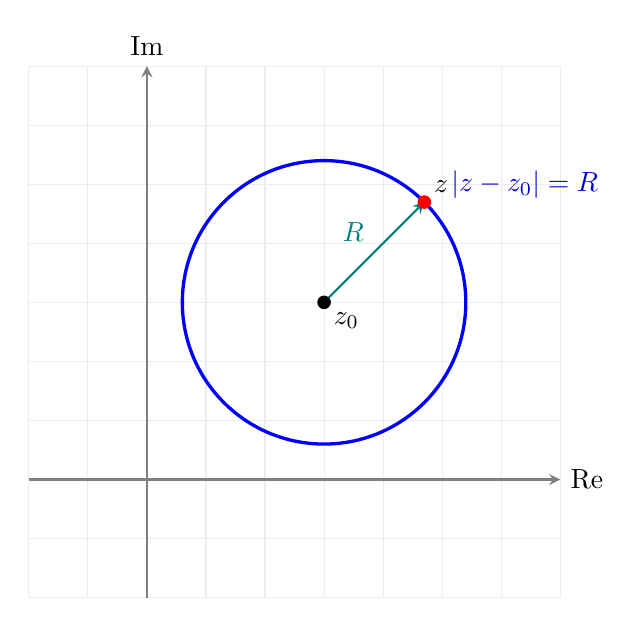
\begin{tikzpicture}[scale=1.5, >=stealth]
    % Grid lines
    \draw[color=gray!15, thin, step=0.5] (-1,-1) grid (3.5,3.5);
    
    % Axes
    \draw[->, thick, gray] (-1,0) -- (3.5,0) node[right, text=black] {$\text{Re}$};
    \draw[->, thick, gray] (0,-1) -- (0,3.5) node[above, text=black] {$\text{Im}$};

    % Center and Circle Parameters
    \coordinate (Z0) at (1.5, 1.5);
    \def\R{1.2}; % Radius

    % Draw the circle
    \draw[very thick, blue] (Z0) circle (\R);

    % Draw a point z on the circle
    \coordinate (Z) at ($(Z0) + (45:\R)$);
    
    % Radius vector
    \draw[->, thick, teal] (Z0) -- (Z) node[midway, above left] {$R$};
    
    % Points
    \filldraw[black] (Z0) circle (1.5pt) node[below right] {$z_0$};
    \filldraw[red] (Z) circle (1.5pt) node[above right, text=black] {$z$};

    % Locus label
    \node[blue!80!black] at (3.2, 2.5) {$|z - z_0| = R$};

\end{tikzpicture}
\end{center}

\end{tcolorbox}

\item Describe mathematically and graphically the region represented by $z(\bar{z}+2)=3$.
\mk{10} \yr{MATH 241 | L-2/T-1 | 2014--15}

\begin{tcolorbox}[enhanced,breakable,ansbox,colback=cE!4,colframe=cE,boxrule=0.8pt,arc=5pt,title={\textbf{Answer}},fonttitle=\bfseries\color{white},colbacktitle=cE]

\subsection*{1. Mathematical Description}

To find the region represented by the equation $z(\bar{z}+2)=3$, we express the complex number $z$ in its rectangular form, $z = x + iy$, where $x$ and $y$ are real numbers. The complex conjugate of $z$ is $\bar{z} = x - iy$.

Substitute $z$ and $\bar{z}$ into the given equation:
\begin{align*}
    z(\bar{z} + 2) &= 3 \\
    z\bar{z} + 2z &= 3
\end{align*}

Using the property $z\bar{z} = |z|^2 = x^2 + y^2$, we can rewrite the equation in terms of $x$ and $y$:
\begin{align*}
    (x^2 + y^2) + 2(x + iy) &= 3 \\
    (x^2 + y^2 + 2x) + i(2y) &= 3 + i(0)
\end{align*}

For two complex numbers to be equal, their real parts and imaginary parts must respectively be equal. This gives us a system of two real equations:
\begin{align}
    x^2 + y^2 + 2x &= 3 \\
    2y &= 0 
\end{align}

From Equation (2), it is immediately clear that:
\[
y = 0
\]
This indicates that any solution must lie strictly on the real axis. Substituting $y = 0$ into Equation (1) yields:
\begin{align*}
    x^2 + 0^2 + 2x &= 3 \\
    x^2 + 2x - 3 &= 0
\end{align*}

Factoring the quadratic equation, we obtain:
\[
    (x + 3)(x - 1) = 0
\]
Which gives the roots:
\[
    x = -3 \quad \text{or} \quad x = 1
\]

\textbf{Conclusion:} 
Because the imaginary part $y$ is constrained to be precisely zero, the solution does not form a continuous 2D region or a curve (such as a circle). Instead, the "region" consists entirely of \textbf{two discrete points} on the real axis: 
\begin{equation*}
\boxed{z = 1 \quad \text{and} \quad z = -3}
\end{equation*}

\subsection*{2. Graphical Representation}

Graphically, this set of solutions is represented by plotting the two exact coordinates $(-3, 0)$ and $(1, 0)$ in the complex plane. 

\begin{center}
\begin{tikzpicture}[scale=1.5, >=stealth]
    % Grid lines
    \draw[color=gray!30, thin, step=1.0] (-4.5,-2.5) grid (2.5,2.5);
    
    % Axes
    \draw[->, thick] (-4.5,0) -- (2.8,0) node[right] {$\text{Re}(z)$};
    \draw[->, thick] (0,-2.5) -- (0,2.8) node[above] {$\text{Im}(z)$};
    
    % Tick marks for Re(z)
    \foreach \x in {-4,-3,-2,-1,1,2} {
        \draw (\x, 0.08) -- (\x, -0.08) node[below] {\footnotesize $\x$};
    }
    
    % Tick marks for Im(z)
    \foreach \y in {-2,-1,1,2} {
        \draw (0.08, \y) -- (-0.08, \y) node[left] {\footnotesize $\y i$};
    }
    
    % The two solution points
    \filldraw[red] (1,0) circle (2.5pt) node[above right, text=black] {$z_1 = 1$};
    \filldraw[red] (-3,0) circle (2.5pt) node[above left, text=black] {$z_2 = -3$};
    
    % Highlight that they are on the real axis
    \draw[red, thick, dashed] (-3.5,0) -- (1.5,0);

\end{tikzpicture}
\end{center}

\end{tcolorbox}

\item Prove that $|z_{1}+z_{2}|^{2}+|z_{1}-z_{2}|^{2}=2|z_{1}|^{2}+2|z_{2}|^{2}$ and hence deduce that
\[
\left|a+\sqrt{a^{2}-b^{2}}\right|+\left|a-\sqrt{a^{2}-b^{2}}\right|=|a+b|+|a-b|,
\]
where $z_{1},z_{2},a,b$ are complex numbers.
\mk{20} \yr{MATH 241 | L-2/T-1 | 2013--14}

\begin{tcolorbox}[enhanced,breakable,ansbox,colback=cE!4,colframe=cE,boxrule=0.8pt,arc=5pt,title={\textbf{Answer}},fonttitle=\bfseries\color{white},colbacktitle=cE]

\subsection*{Part 1: Proof of the Parallelogram Law}

Let $z_1$ and $z_2$ be complex numbers. We want to prove the identity:
\[
|z_{1}+z_{2}|^{2}+|z_{1}-z_{2}|^{2}=2|z_{1}|^{2}+2|z_{2}|^{2}
\]
Recall that for any complex number $z$, $|z|^2 = z\bar{z}$, and that the conjugate of a sum is the sum of the conjugates ($\overline{z_1 \pm z_2} = \bar{z}_1 \pm \bar{z}_2$). Expanding the left-hand side (LHS):
\begin{align*}
\text{LHS} &= |z_1 + z_2|^2 + |z_1 - z_2|^2 \\
&= (z_1 + z_2)(\overline{z_1 + z_2}) + (z_1 - z_2)(\overline{z_1 - z_2}) \\
&= (z_1 + z_2)(\bar{z}_1 + \bar{z}_2) + (z_1 - z_2)(\bar{z}_1 - \bar{z}_2)
\end{align*}
Distributing the terms in both products:
\begin{align*}
(z_1 + z_2)(\bar{z}_1 + \bar{z}_2) &= z_1\bar{z}_1 + z_1\bar{z}_2 + z_2\bar{z}_1 + z_2\bar{z}_2 \\
(z_1 - z_2)(\bar{z}_1 - \bar{z}_2) &= z_1\bar{z}_1 - z_1\bar{z}_2 - z_2\bar{z}_1 + z_2\bar{z}_2
\end{align*}
Adding these two expressions, the cross terms $z_1\bar{z}_2$ and $z_2\bar{z}_1$ cancel out perfectly:
\begin{align*}
\text{LHS} &= 2z_1\bar{z}_1 + 2z_2\bar{z}_2 \\
&= 2|z_1|^2 + 2|z_2|^2 = \text{RHS}
\end{align*}
This proves the identity. $\blacksquare$

\vspace{10pt}
\begin{center}
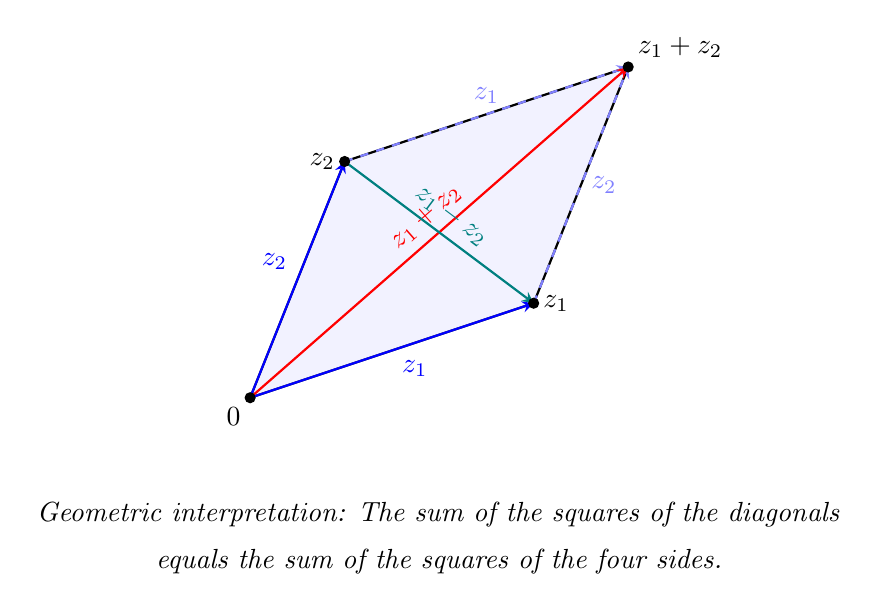
\begin{tikzpicture}[scale=1.2, >=stealth]
    % Coordinates
    \coordinate (O) at (0,0);
    \coordinate (Z1) at (3, 1);
    \coordinate (Z2) at (1, 2.5);
    \coordinate (Z1Z2) at (4, 3.5); % Z1 + Z2

    % Draw Parallelogram
    \draw[thick, fill=blue!5] (O) -- (Z1) -- (Z1Z2) -- (Z2) -- cycle;
    
    % Draw vectors (Sides)
    \draw[->, thick, blue] (O) -- (Z1) node[midway, below right] {$z_1$};
    \draw[->, thick, blue] (O) -- (Z2) node[midway, above left] {$z_2$};
    \draw[->, thick, blue!50, dashed] (Z1) -- (Z1Z2) node[midway, right] {$z_2$};
    \draw[->, thick, blue!50, dashed] (Z2) -- (Z1Z2) node[midway, above] {$z_1$};

    % Draw Diagonals
    \draw[->, thick, red] (O) -- (Z1Z2) node[midway, sloped, above] {$z_1 + z_2$};
    \draw[->, thick, teal] (Z2) -- (Z1) node[midway, sloped, above] {$z_1 - z_2$};

    % Points
    \filldraw (O) circle (1.5pt) node[below left] {$0$};
    \filldraw (Z1) circle (1.5pt) node[right] {$z_1$};
    \filldraw (Z2) circle (1.5pt) node[left] {$z_2$};
    \filldraw (Z1Z2) circle (1.5pt) node[above right] {$z_1+z_2$};
    
    % Annotation
    \node[anchor=north] at (2,-1) {\textit{Geometric interpretation: The sum of the squares of the diagonals}};
    \node[anchor=north] at (2,-1.5) {\textit{equals the sum of the squares of the four sides.}};
\end{tikzpicture}
\end{center}

\vspace{10pt}

\subsection*{Part 2: Deduction of the Target Equation}

Let $u = a+\sqrt{a^{2}-b^{2}}$ and $v = a-\sqrt{a^{2}-b^{2}}$. 
We want to evaluate the quantity $(|u| + |v|)^2$:
\begin{equation}
(|u| + |v|)^2 = |u|^2 + |v|^2 + 2|u||v| = |u|^2 + |v|^2 + 2|uv|
\label{eq:uv_squared}
\end{equation}

First, we calculate $|u|^2 + |v|^2$ using the Parallelogram Law proved in Part 1. Notice that:
\begin{align*}
u + v &= \left(a+\sqrt{a^{2}-b^{2}}\right) + \left(a-\sqrt{a^{2}-b^{2}}\right) = 2a \\
u - v &= \left(a+\sqrt{a^{2}-b^{2}}\right) - \left(a-\sqrt{a^{2}-b^{2}}\right) = 2\sqrt{a^{2}-b^{2}}
\end{align*}
By the Parallelogram Law applied to $u$ and $v$:
\begin{align*}
2|u|^2 + 2|v|^2 &= |u+v|^2 + |u-v|^2 \\
2(|u|^2 + |v|^2) &= |2a|^2 + |2\sqrt{a^2-b^2}|^2 \\
2(|u|^2 + |v|^2) &= 4|a|^2 + 4|a^2-b^2| \\
|u|^2 + |v|^2 &= 2|a|^2 + 2|a^2-b^2|
\end{align*}

Next, we evaluate the product term $uv$:
\begin{align*}
uv &= \left(a+\sqrt{a^{2}-b^{2}}\right)\left(a-\sqrt{a^{2}-b^{2}}\right) \\
&= a^2 - \left(\sqrt{a^2-b^2}\right)^2 = a^2 - (a^2 - b^2) = b^2
\end{align*}
Thus, $2|uv| = 2|b^2| = 2|b|^2$.

Substitute these back into Equation \eqref{eq:uv_squared}:
\begin{equation}
(|u| + |v|)^2 = 2|a|^2 + 2|a^2-b^2| + 2|b|^2
\label{eq:LHS_expanded}
\end{equation}

Now, consider the right-hand side of the target equation, $|a+b| + |a-b|$, and square it:
\begin{align*}
(|a+b| + |a-b|)^2 &= |a+b|^2 + |a-b|^2 + 2|a+b||a-b| \\
&= \left( |a+b|^2 + |a-b|^2 \right) + 2|(a+b)(a-b)| \\
&= \left( |a+b|^2 + |a-b|^2 \right) + 2|a^2 - b^2|
\end{align*}
Apply the Parallelogram Law again, this time directly to $a$ and $b$:
\[
|a+b|^2 + |a-b|^2 = 2|a|^2 + 2|b|^2
\]
Substituting this into our expansion:
\begin{equation}
(|a+b| + |a-b|)^2 = 2|a|^2 + 2|b|^2 + 2|a^2 - b^2|
\label{eq:RHS_expanded}
\end{equation}

Comparing Equation \eqref{eq:LHS_expanded} and Equation \eqref{eq:RHS_expanded}, we clearly see that:
\[
(|u| + |v|)^2 = (|a+b| + |a-b|)^2
\]
Since $|u| + |v|$ and $|a+b| + |a-b|$ are both sums of moduli, they are strictly non-negative real numbers. Therefore, taking the principal square root of both sides yields:
\[
|u| + |v| = |a+b| + |a-b|
\]
Substituting $u$ and $v$ back gives the desired result:
\begin{equation*}
\boxed{\left|a+\sqrt{a^{2}-b^{2}}\right|+\left|a-\sqrt{a^{2}-b^{2}}\right|=|a+b|+|a-b|}
\end{equation*}

\end{tcolorbox}

\item Describe mathematically and graphically the region represented by $|z+2-3i|+|z-2+3i|<10$.
\mk{5} \yr{MATH 241 | L-2/T-1 | 2013--14}

\begin{tcolorbox}[enhanced,breakable,ansbox,colback=cE!4,colframe=cE,boxrule=0.8pt,arc=5pt,title={\textbf{Answer}},fonttitle=\bfseries\color{white},colbacktitle=cE]

\subsection*{1. Mathematical Description}

The given inequality is:
\[
|z+2-3i| + |z-2+3i| < 10
\]
First, we rewrite the terms inside the absolute values to highlight the geometric meaning of modulus as distance:
\[
|z - (-2 + 3i)| + |z - (2 - 3i)| < 10
\]
Let $z_1 = -2 + 3i$ and $z_2 = 2 - 3i$. The expression $|z - z_1| + |z - z_2|$ represents the sum of the distances from a point $z$ to two fixed points, $z_1$ and $z_2$, in the complex plane. 

Recall that the locus of points $z$ such that the sum of the distances to two fixed points (the foci) is a constant $2a$ is an \textbf{ellipse}. 
Here, the constant sum is bounded by $2a = 10$, which implies $a = 5$. Because the inequality is strictly less than ($<$), the region represents the \textbf{interior} of this ellipse, excluding its boundary.

We can determine the key geometric properties of this ellipse:
\begin{itemize}
    \item \textbf{Foci:} The foci are located at $z_1 = -2 + 3i$ and $z_2 = 2 - 3i$.
    \item \textbf{Center:} The center $z_c$ is the midpoint of the segment connecting the foci:
    \[
    z_c = \frac{z_1 + z_2}{2} = \frac{(-2 + 3i) + (2 - 3i)}{2} = 0
    \]
    So, the ellipse is centered at the origin $(0,0)$.
    \item \textbf{Focal Distance ($c$):} The distance from the center to a focus is $c = |z_1 - z_c|$:
    \[
    c = |-2 + 3i| = \sqrt{(-2)^2 + 3^2} = \sqrt{4 + 9} = \sqrt{13}
    \]
    \item \textbf{Semi-minor Axis ($b$):} Using the ellipse relationship $a^2 = b^2 + c^2$:
    \[
    b^2 = a^2 - c^2 = 5^2 - (\sqrt{13})^2 = 25 - 13 = 12 \implies b = \sqrt{12} = 2\sqrt{3}
    \]
\end{itemize}

\textbf{Conclusion:} Mathematically, the region is the strictly open interior of an ellipse centered at the origin, with semi-major axis $a = 5$, semi-minor axis $b = 2\sqrt{3}$, and its major axis passing through the foci $(-2, 3)$ and $(2, -3)$.

\vspace{10pt}

\subsection*{2. Graphical Representation}

The angle of inclination of the major axis is $\tan^{-1}\left(\frac{-3 - 3}{2 - (-2)}\right) = \tan^{-1}\left(-\frac{6}{4}\right) \approx -56.3^\circ$. The boundary is drawn with a dashed line to indicate the strict inequality ($< 10$).

\begin{center}
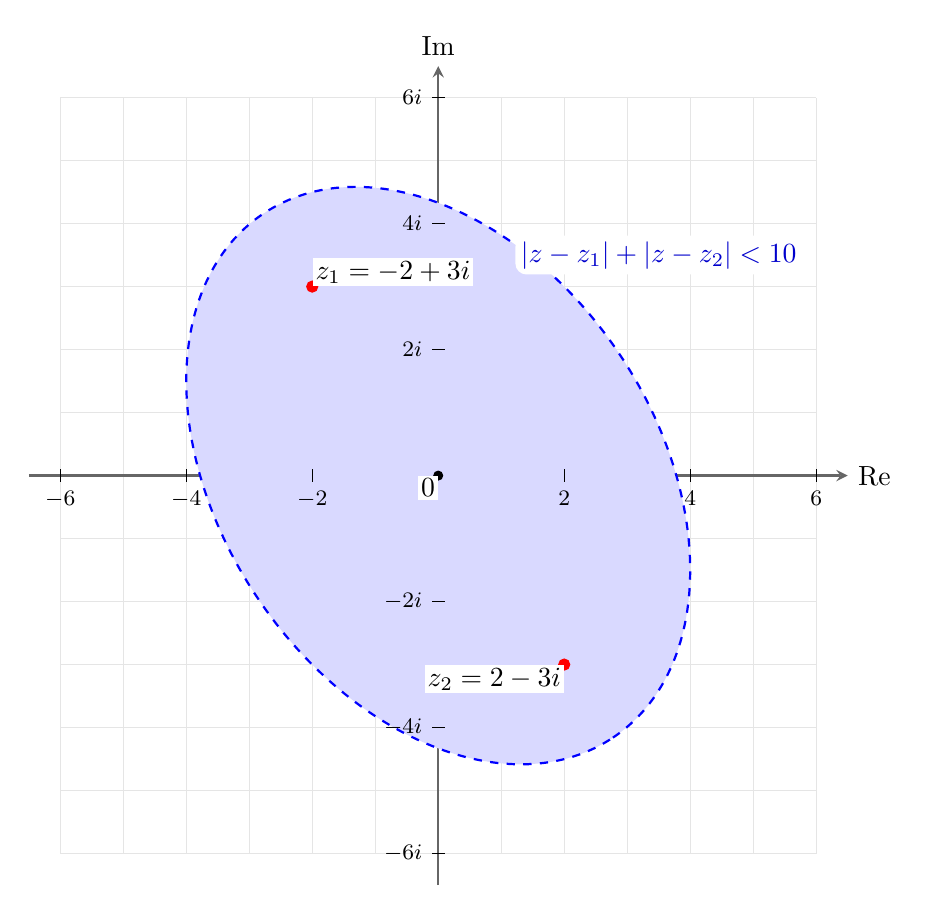
\begin{tikzpicture}[scale=0.8, >=stealth]
    % Grid
    \draw[color=gray!20, thin, step=1] (-6,-6) grid (6,6);
    
    % Axes
    \draw[->, thick, gray!80!black] (-6.5,0) -- (6.5,0) node[right, text=black] {$\text{Re}$};
    \draw[->, thick, gray!80!black] (0,-6.5) -- (0,6.5) node[above, text=black] {$\text{Im}$};

    % Ellipse: Center (0,0), a=5, b=sqrt(12)≈3.464, angle atan(-1.5) ≈ -56.31 degrees
    \filldraw[fill=blue!15, draw=blue, thick, dashed, rotate=-56.31] (0,0) ellipse (5 and 3.464);

    % Axis ticks
    \foreach \x in {-6,-4,-2,2,4,6} {
        \draw (\x, 0.1) -- (\x, -0.1) node[below] {\footnotesize $\x$};
    }
    \foreach \y in {-6,-4,-2,2,4,6} {
        \draw (0.1, \y) -- (-0.1, \y) node[left] {\footnotesize $\y i$};
    }

    % Foci
    \filldraw[red] (-2,3) circle (2.5pt) node[above right, text=black, fill=white, inner sep=1pt] {$z_1 = -2+3i$};
    \filldraw[red] (2,-3) circle (2.5pt) node[below left, text=black, fill=white, inner sep=1pt] {$z_2 = 2-3i$};

    % Center
    \filldraw[black] (0,0) circle (2pt) node[below left, fill=white, inner sep=1pt] {$0$};

    % Add region label
    \node[blue!80!black, fill=white, inner sep=2pt, rounded corners] at (3.5, 3.5) {$|z-z_1| + |z-z_2| < 10$};

\end{tikzpicture}
\end{center}

\end{tcolorbox}

\item Prove the triangle inequalities of complex numbers:
\begin{enumerate}
  \item $|z_{1}+z_{2}| \le |z_{1}|+|z_{2}|$
  \item $|z_{1}-z_{2}| \ge \bigl||z_{1}|-|z_{2}|\bigr|$
\end{enumerate}
\mk{17} \yr{MATH 241 | L-2/T-1 | 2012--13}

\begin{tcolorbox}[enhanced,breakable,ansbox,colback=cE!4,colframe=cE,boxrule=0.8pt,arc=5pt,title={\textbf{Answer}},fonttitle=\bfseries\color{white},colbacktitle=cE]

\subsection*{Part 1: Prove that $|z_{1}+z_{2}| \le |z_{1}|+|z_{2}|$}

Let $z_1$ and $z_2$ be two complex numbers. We begin by considering the square of the modulus of their sum, $|z_1 + z_2|^2$. Using the property that $|w|^2 = w\bar{w}$ for any complex number $w$, we have:
\begin{align*}
|z_1 + z_2|^2 &= (z_1 + z_2)\overline{(z_1 + z_2)} \\
&= (z_1 + z_2)(\bar{z}_1 + \bar{z}_2)
\end{align*}
Expanding the product, we get:
\begin{align*}
|z_1 + z_2|^2 &= z_1\bar{z}_1 + z_1\bar{z}_2 + z_2\bar{z}_1 + z_2\bar{z}_2 \\
&= |z_1|^2 + z_1\bar{z}_2 + \bar{z}_1z_2 + |z_2|^2
\end{align*}
Notice that $\bar{z}_1z_2$ is the complex conjugate of $z_1\bar{z}_2$, because $\overline{z_1\bar{z}_2} = \bar{z}_1\overline{\bar{z}_2} = \bar{z}_1z_2$. 
Recall that for any complex number $w$, the sum of the number and its conjugate is twice its real part: $w + \bar{w} = 2\operatorname{Re}(w)$. Letting $w = z_1\bar{z}_2$, we can write:
\[
z_1\bar{z}_2 + \bar{z}_1z_2 = 2\operatorname{Re}(z_1\bar{z}_2)
\]
Substituting this back into our equation gives:
\begin{equation}
|z_1 + z_2|^2 = |z_1|^2 + 2\operatorname{Re}(z_1\bar{z}_2) + |z_2|^2
\end{equation}
We know that the real part of any complex number is less than or equal to its modulus, so $\operatorname{Re}(z_1\bar{z}_2) \le |z_1\bar{z}_2|$. Furthermore, $|z_1\bar{z}_2| = |z_1||\bar{z}_2| = |z_1||z_2|$. Thus:
\[
\operatorname{Re}(z_1\bar{z}_2) \le |z_1||z_2|
\]
Applying this inequality to equation (1):
\begin{align*}
|z_1 + z_2|^2 &\le |z_1|^2 + 2|z_1||z_2| + |z_2|^2 \\
|z_1 + z_2|^2 &\le (|z_1| + |z_2|)^2
\end{align*}
Since the moduli are non-negative real numbers, taking the principal square root of both sides yields the forward triangle inequality:
\begin{equation*}
\boxed{|z_{1}+z_{2}| \le |z_{1}|+|z_{2}|}
\end{equation*}

---

\subsection*{Part 2: Prove that $|z_{1}-z_{2}| \ge \bigl||z_{1}|-|z_{2}|\bigr|$}

We can prove this by cleverly applying the forward triangle inequality established in Part 1. 

\textbf{Step 1:} Express $z_1$ in terms of $z_1 - z_2$ and $z_2$:
\[
z_1 = (z_1 - z_2) + z_2
\]
Applying the result from Part 1 to the sum on the right side:
\[
|z_1| = |(z_1 - z_2) + z_2| \le |z_1 - z_2| + |z_2|
\]
Subtracting $|z_2|$ from both sides provides our first key inequality:
\begin{equation}
|z_1| - |z_2| \le |z_1 - z_2|
\end{equation}

\textbf{Step 2:} Now, we swap the roles of $z_1$ and $z_2$. Express $z_2$ as:
\[
z_2 = (z_2 - z_1) + z_1
\]
Applying the triangle inequality again:
\[
|z_2| = |(z_2 - z_1) + z_1| \le |z_2 - z_1| + |z_1|
\]
Recall that the modulus of a complex number and its negative are equal, so $|z_2 - z_1| = |-(z_1 - z_2)| = |z_1 - z_2|$. Therefore:
\[
|z_2| \le |z_1 - z_2| + |z_1|
\]
Subtracting $|z_1|$ from both sides yields:
\[
|z_2| - |z_1| \le |z_1 - z_2|
\]
Multiplying the left side by $-1$ gives our second key inequality:
\begin{equation}
-(|z_1| - |z_2|) \le |z_1 - z_2|
\end{equation}

\textbf{Step 3:} Equations (2) and (3) establish that both $(|z_1| - |z_2|)$ and its negative are less than or equal to $|z_1 - z_2|$. By the definition of absolute value for real numbers, this directly implies:
\begin{equation*}
\boxed{|z_1 - z_2| \ge \bigl||z_1| - |z_2|\bigr|}
\end{equation*}
Thus, the reverse triangle inequality is proven. $\blacksquare$

---

\subsection*{Geometric Interpretation}

In the complex plane, complex numbers add via the parallelogram law (equivalent to vector addition). The points $0$, $z_1$, and $z_1+z_2$ form a triangle. The lengths of the sides are $|z_1|$, $|z_2|$, and $|z_1+z_2|$. 

\begin{itemize}
    \item \textbf{Forward Inequality:} The length of any one side of a triangle must be less than or equal to the sum of the lengths of the other two sides.
    \item \textbf{Reverse Inequality:} The length of any one side must be greater than or equal to the absolute difference of the lengths of the other two sides.
\end{itemize}

\begin{center}
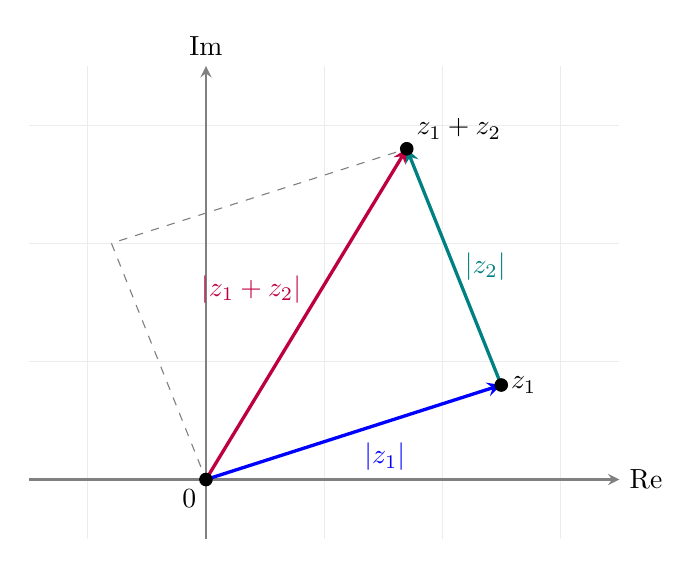
\begin{tikzpicture}[scale=1.5, >=stealth]
    % Grid lines (optional, kept light)
    \draw[color=gray!15, thin, step=1] (-1.5,-0.5) grid (3.5,3.5);
    
    % Axes
    \draw[->, thick, gray] (-1.5,0) -- (3.5,0) node[right, text=black] {$\text{Re}$};
    \draw[->, thick, gray] (0,-0.5) -- (0,3.5) node[above, text=black] {$\text{Im}$};

    % Coordinates for the vectors
    \coordinate (O) at (0,0);
    \coordinate (Z1) at (2.5, 0.8);
    \coordinate (Z2) at (-0.8, 2.0);
    \coordinate (Z1Z2) at (1.7, 2.8); % Z1 + Z2

    % Parallelogram (dashed) for context
    \draw[dashed, gray] (Z1) -- (Z1Z2) -- (Z2) -- (O);

    % Vectors forming the main triangle O -> Z1 -> Z1Z2
    \draw[->, line width=1.2pt, blue] (O) -- (Z1) node[midway, below right] {$|z_1|$};
    \draw[->, line width=1.2pt, teal] (Z1) -- (Z1Z2) node[midway, right] {$|z_2|$};
    
    % Resultant Vector
    \draw[->, line width=1.2pt, purple] (O) -- (Z1Z2) node[midway, above left, xshift=2pt] {$|z_1+z_2|$};

    % Points and Labels
    \filldraw[black] (O) circle (1.5pt) node[below left] {$0$};
    \filldraw[black] (Z1) circle (1.5pt) node[right] {$z_1$};
    \filldraw[black] (Z1Z2) circle (1.5pt) node[above right] {$z_1+z_2$};

\end{tikzpicture}
\end{center}

\end{tcolorbox}

\item Show that the equation $\left|z+\dfrac{1}{z}\right|=2$ represents two circles with centres $(0,1)$, $(0,-1)$ and radius $\sqrt{2}$.
\mk{10} \yr{MATH 241 | L-2/T-1 | 2011--12}

\begin{tcolorbox}[enhanced,breakable,ansbox,colback=cE!4,colframe=cE,boxrule=0.8pt,arc=5pt,title={\textbf{Answer}},fonttitle=\bfseries\color{white},colbacktitle=cE]

\subsection*{1. Algebraic Expansion}

Let the complex number be $z = x + iy$. We can express its reciprocal as:
\[
\frac{1}{z} = \frac{\bar{z}}{|z|^2} = \frac{x - iy}{x^2 + y^2}
\]
Substitute this into the expression $z + \frac{1}{z}$:
\begin{align*}
z + \frac{1}{z} &= (x + iy) + \left(\frac{x}{x^2 + y^2} - i\frac{y}{x^2 + y^2}\right) \\
&= \left(x + \frac{x}{x^2 + y^2}\right) + i\left(y - \frac{y}{x^2 + y^2}\right)
\end{align*}
We are given that $\left|z + \frac{1}{z}\right| = 2$. Squaring both sides gives $\left|z + \frac{1}{z}\right|^2 = 4$. Using the real and imaginary parts derived above, we obtain:
\begin{equation}
\left(x + \frac{x}{x^2 + y^2}\right)^2 + \left(y - \frac{y}{x^2 + y^2}\right)^2 = 4
\label{eq:expanded}
\end{equation}

To simplify, let $r^2 = x^2 + y^2$. Equation \eqref{eq:expanded} becomes:
\begin{align*}
x^2\left(1 + \frac{1}{r^2}\right)^2 + y^2\left(1 - \frac{1}{r^2}\right)^2 &= 4 \\
x^2\left(1 + \frac{2}{r^2} + \frac{1}{r^4}\right) + y^2\left(1 - \frac{2}{r^2} + \frac{1}{r^4}\right) &= 4 \\
(x^2 + y^2) + \frac{2(x^2 - y^2)}{r^2} + \frac{x^2 + y^2}{r^4} &= 4
\end{align*}
Substitute $x^2 + y^2$ back with $r^2$:
\begin{align*}
r^2 + \frac{2(x^2 - y^2)}{r^2} + \frac{r^2}{r^4} &= 4 \\
r^2 + \frac{2(x^2 - y^2)}{r^2} + \frac{1}{r^2} &= 4
\end{align*}
Multiply the entire equation by $r^2$ to clear the denominators:
\[
r^4 + 2(x^2 - y^2) + 1 = 4r^2
\]

\subsection*{2. Factorization}

Now substitute $r^2 = x^2 + y^2$ back into the equation:
\begin{align*}
(x^2 + y^2)^2 + 2x^2 - 2y^2 + 1 &= 4(x^2 + y^2) \\
(x^2 + y^2)^2 + 2x^2 - 2y^2 + 1 - 4x^2 - 4y^2 &= 0 \\
(x^2 + y^2)^2 - 2x^2 - 6y^2 + 1 &= 0
\end{align*}
To factor this elegantly, we can rewrite the terms to form a perfect square:
\begin{align*}
(x^2 + y^2)^2 - 2(x^2 + y^2) + 1 - 4y^2 &= 0 \\
\left( (x^2 + y^2) - 1 \right)^2 - (2y)^2 &= 0
\end{align*}
This is a difference of squares, $A^2 - B^2 = (A-B)(A+B)$, which factors as:
\[
(x^2 + y^2 - 1 - 2y)(x^2 + y^2 - 1 + 2y) = 0
\]
This implies that the locus consists of two separate equations:
\begin{align*}
\text{Equation 1: } & x^2 + y^2 - 2y - 1 = 0 \\
\text{Equation 2: } & x^2 + y^2 + 2y - 1 = 0
\end{align*}

Completing the square for $y$ in both equations:
\begin{align*}
x^2 + (y^2 - 2y + 1) - 1 - 1 = 0 &\implies \boxed{x^2 + (y - 1)^2 = 2} \\
x^2 + (y^2 + 2y + 1) - 1 - 1 = 0 &\implies \boxed{x^2 + (y + 1)^2 = 2}
\end{align*}
These equations represent two circles:
\begin{itemize}
    \item The first circle is centered at $(0, 1)$ with radius $R = \sqrt{2}$.
    \item The second circle is centered at $(0, -1)$ with radius $R = \sqrt{2}$.
\end{itemize}
Thus, the statement is proven. $\blacksquare$

\vspace{10pt}

\subsection*{3. Geometric Visualization}

The two circles intersect exactly on the real axis at $z = 1$ and $z = -1$.

\begin{center}
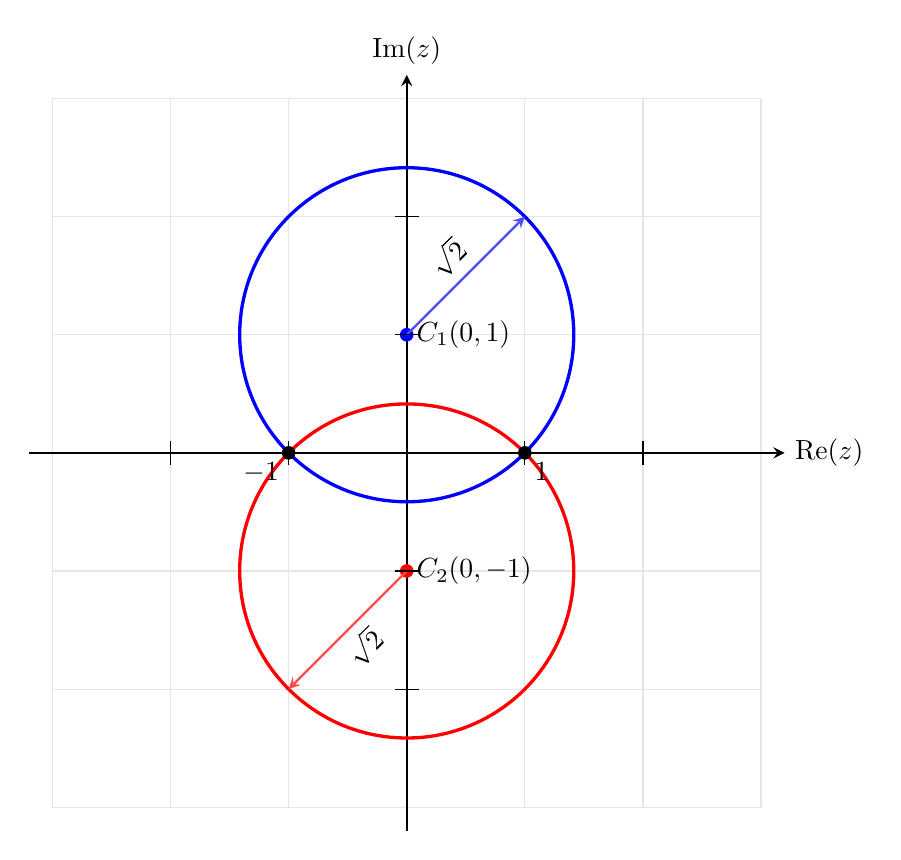
\begin{tikzpicture}[scale=1.5, >=stealth]
    % Grid lines
    \draw[color=gray!20, thin, step=1] (-3,-3) grid (3,3);
    
    % Axes
    \draw[->, thick] (-3.2,0) -- (3.2,0) node[right] {$\text{Re}(z)$};
    \draw[->, thick] (0,-3.2) -- (0,3.2) node[above] {$\text{Im}(z)$};

    % Circle 1: Center (0,1), Radius sqrt(2) ≈ 1.414
    \draw[very thick, blue] (0,1) circle ({sqrt(2)});
    
    % Circle 2: Center (0,-1), Radius sqrt(2) ≈ 1.414
    \draw[very thick, red] (0,-1) circle ({sqrt(2)});

    % Centers
    \filldraw[blue] (0,1) circle (1.5pt) node[right, text=black] {$C_1(0,1)$};
    \filldraw[red] (0,-1) circle (1.5pt) node[right, text=black] {$C_2(0,-1)$};
    
    % Intersections
    \filldraw[black] (1,0) circle (1.5pt) node[below right] {$1$};
    \filldraw[black] (-1,0) circle (1.5pt) node[below left] {$-1$};
    
    % Radius lines
    \draw[->, thick, blue!70!white] (0,1) -- ({sqrt(2)*cos(45)}, {1+sqrt(2)*sin(45)}) node[midway, sloped, above, text=black] {$\sqrt{2}$};
    \draw[->, thick, red!70!white] (0,-1) -- ({-sqrt(2)*cos(45)}, {-1-sqrt(2)*sin(45)}) node[midway, sloped, below, text=black] {$\sqrt{2}$};

    % Tick marks
    \foreach \x in {-2,-1,1,2} \draw (\x, 0.1) -- (\x, -0.1);
    \foreach \y in {-2,-1,1,2} \draw (0.1, \y) -- (-0.1, \y);
\end{tikzpicture}
\end{center}

\end{tcolorbox}

\end{enumerate}

%%──────────────────────────────────────────────────────────────────────
\subtopic{cE}{Roots of Complex Numbers}
\label{sub:s5-roots}

\begin{enumerate}

    
\item Find all roots of $(-8)^{1/6}$ in rectangular coordinates, exhibit them as vertices of a regular polygon, and identify the principal root.
\mk{10} \yr{MATH 245 | L-2/T-1 | 2021--22}

    \begin{tcolorbox}[enhanced,breakable,ansbox,colback=cE!4,colframe=cE,boxrule=0.8pt,arc=5pt,title={\textbf{Answer}},fonttitle=\bfseries\color{white},colbacktitle=cE]

To find all the 6th roots of $-8$, we first express the complex number $z = -8$ in its polar form. 
The magnitude is $r = |-8| = 8$, and the argument is $\theta = \pi + 2k\pi$ for any integer $k$. Thus, we can write:
\[ z = 8 e^{i(\pi + 2k\pi)} \]

The 6th roots of $z$ are given by the formula:
\[ w_k = z^{1/6} = 8^{1/6} e^{i \left( \frac{\pi + 2k\pi}{6} \right)} = \sqrt{2} e^{i \left( \frac{\pi}{6} + \frac{k\pi}{3} \right)} \]
for $k = 0, 1, 2, 3, 4, 5$.

Now, we evaluate each root and convert it to rectangular coordinates ($x + iy$) using Euler's formula $e^{i\theta} = \cos\theta + i\sin\theta$:

\begin{align*}
    k=0: \quad w_0 &= \sqrt{2} \left( \cos\frac{\pi}{6} + i\sin\frac{\pi}{6} \right) = \sqrt{2} \left( \frac{\sqrt{3}}{2} + i\frac{1}{2} \right) = \frac{\sqrt{6}}{2} + i\frac{\sqrt{2}}{2} \\
    k=1: \quad w_1 &= \sqrt{2} \left( \cos\frac{\pi}{2} + i\sin\frac{\pi}{2} \right) = \sqrt{2} \left( 0 + i(1) \right) = i\sqrt{2} \\
    k=2: \quad w_2 &= \sqrt{2} \left( \cos\frac{5\pi}{6} + i\sin\frac{5\pi}{6} \right) = \sqrt{2} \left( -\frac{\sqrt{3}}{2} + i\frac{1}{2} \right) = -\frac{\sqrt{6}}{2} + i\frac{\sqrt{2}}{2} \\
    k=3: \quad w_3 &= \sqrt{2} \left( \cos\frac{7\pi}{6} + i\sin\frac{7\pi}{6} \right) = \sqrt{2} \left( -\frac{\sqrt{3}}{2} - i\frac{1}{2} \right) = -\frac{\sqrt{6}}{2} - i\frac{\sqrt{2}}{2} \\
    k=4: \quad w_4 &= \sqrt{2} \left( \cos\frac{3\pi}{2} + i\sin\frac{3\pi}{2} \right) = \sqrt{2} \left( 0 - i(1) \right) = -i\sqrt{2} \\
    k=5: \quad w_5 &= \sqrt{2} \left( \cos\frac{11\pi}{6} + i\sin\frac{11\pi}{6} \right) = \sqrt{2} \left( \frac{\sqrt{3}}{2} - i\frac{1}{2} \right) = \frac{\sqrt{6}}{2} - i\frac{\sqrt{2}}{2}
\end{align*}

\textbf{Principal Root:}
The principal root of a complex number corresponds to the principal argument $\text{Arg}(z) \in (-\pi, \pi]$. For $z = -8$, the principal argument is $\pi$. The principal $n$-th root is obtained by evaluating $k=0$ using the principal argument. Therefore, the principal root is:
\[ \boxed{w_0 = \frac{\sqrt{6}}{2} + i\frac{\sqrt{2}}{2}} \]

\vspace{1em}
\textbf{Geometric Representation:}
The six roots lie on a circle of radius $R = \sqrt{2} \approx 1.414$ centered at the origin in the complex plane. Because they are evenly spaced by an angle of $\frac{2\pi}{6} = \frac{\pi}{3} = 60^\circ$, they form the vertices of a regular hexagon.

\begin{center}
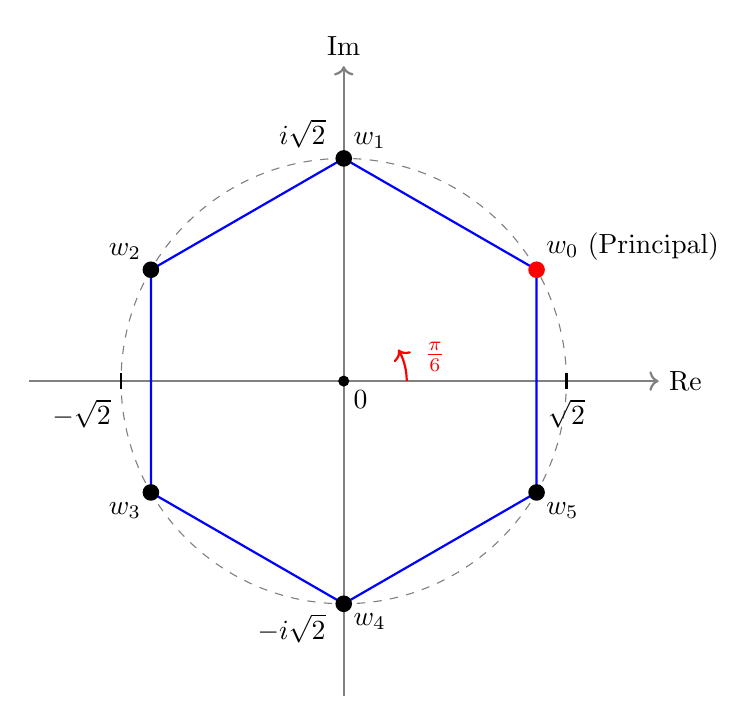
\begin{tikzpicture}[scale=2]
    % Draw axes
    \draw[->, gray, thick] (-2, 0) -- (2, 0) node[right, text=black] {$\text{Re}$};
    \draw[->, gray, thick] (0, -2) -- (0, 2) node[above, text=black] {$\text{Im}$};
    
    % Draw circle of radius sqrt(2)
    \draw[dashed, gray] (0,0) circle (1.414);
    
    % Draw the regular hexagon
    \draw[thick, blue] (30:1.414) \foreach \ang in {90, 150, 210, 270, 330} { -- (\ang:1.414) } -- cycle;
    
    % Plot and label the roots
    \fill[red] (30:1.414) circle (1.5pt) node[above right, black] {$w_0$ (Principal)};
    \fill[black] (90:1.414) circle (1.5pt) node[above right] {$w_1$};
    \fill[black] (150:1.414) circle (1.5pt) node[above left] {$w_2$};
    \fill[black] (210:1.414) circle (1.5pt) node[below left] {$w_3$};
    \fill[black] (270:1.414) circle (1.5pt) node[below right] {$w_4$};
    \fill[black] (330:1.414) circle (1.5pt) node[below right] {$w_5$};
    
    % Origin
    \fill[black] (0,0) circle (1pt) node[below right] {$0$};
    
    % Tick marks for radius
    \draw[thick] (1.414, 0.05) -- (1.414, -0.05) node[below] {$\sqrt{2}$};
    \draw[thick] (-1.414, 0.05) -- (-1.414, -0.05) node[below left] {$-\sqrt{2}$};
    \draw[thick] (0.05, 1.414) -- (-0.05, 1.414) node[above left] {$i\sqrt{2}$};
    \draw[thick] (0.05, -1.414) -- (-0.05, -1.414) node[below left] {$-i\sqrt{2}$};

    % Angle arc for principal root
    \draw[->, red, thick] (0.4, 0) arc (0:30:0.4);
    \node[red] at (15:0.6) {$\frac{\pi}{6}$};
\end{tikzpicture}
\end{center}

\end{tcolorbox}
    
\item Find all the roots of $(-2\sqrt{3}-2i)^{1/4}$ in rectangular coordinates and exhibit the distinct roots graphically.
\mk{10} \yr{MATH 241 | L-2/T-1 | 2013--14, 2011--12}

\begin{tcolorbox}[enhanced,breakable,ansbox,colback=cE!4,colframe=cE,boxrule=0.8pt,arc=5pt,title={\textbf{Answer}},fonttitle=\bfseries\color{white},colbacktitle=cE]

\subsection*{1. Polar Form of the Complex Number}

Let the given complex number be $w = -2\sqrt{3} - 2i$. To find its roots, we first convert $w$ into its polar form, $w = r(\cos \theta + i \sin \theta) = re^{i\theta}$.

The modulus $r$ is given by:
\[
r = |w| = \sqrt{(-2\sqrt{3})^2 + (-2)^2} = \sqrt{12 + 4} = \sqrt{16} = 4
\]

The argument $\theta$ is found using the real and imaginary parts. Since both the real part ($-2\sqrt{3}$) and the imaginary part ($-2$) are negative, the complex number lies in the third quadrant.
\[
\tan \alpha = \left| \frac{-2}{-2\sqrt{3}} \right| = \frac{1}{\sqrt{3}} \implies \alpha = \frac{\pi}{6}
\]
Thus, the principal argument (or a valid positive argument) is:
\[
\theta = \pi + \frac{\pi}{6} = \frac{7\pi}{6}
\]
So, the polar form of $w$ is:
\[
w = 4 \exp\left(i \frac{7\pi}{6}\right)
\]

\subsection*{2. Finding the Fourth Roots}

We are looking for $z = w^{1/4}$. According to De Moivre's formula for roots, the $n$-th roots of a complex number $re^{i\theta}$ are given by:
\[
z_k = r^{1/n} \exp\left( i \frac{\theta + 2k\pi}{n} \right) \quad \text{for } k = 0, 1, 2, \dots, n-1
\]
For $n = 4$:
\[
r^{1/4} = 4^{1/4} = (2^2)^{1/4} = 2^{1/2} = \sqrt{2}
\]
The angles for the roots are:
\[
\theta_k = \frac{\frac{7\pi}{6} + 2k\pi}{4} = \frac{7\pi}{24} + \frac{k\pi}{2} = \frac{7\pi + 12k\pi}{24}
\]

\subsection*{3. Roots in Rectangular Coordinates}

We evaluate $z_k = x_k + iy_k = \sqrt{2}(\cos \theta_k + i \sin \theta_k)$ for $k = 0, 1, 2, 3$.

\begin{align*}
\textbf{For } k=0: \quad \theta_0 &= \frac{7\pi}{24} \\
z_0 &= \sqrt{2}\cos\left(\frac{7\pi}{24}\right) + i\sqrt{2}\sin\left(\frac{7\pi}{24}\right) \\
&\approx 0.862 + 1.122i \\[8pt]
\textbf{For } k=1: \quad \theta_1 &= \frac{19\pi}{24} \\
z_1 &= \sqrt{2}\cos\left(\frac{19\pi}{24}\right) + i\sqrt{2}\sin\left(\frac{19\pi}{24}\right) \\
&\approx -1.122 + 0.862i \\[8pt]
\textbf{For } k=2: \quad \theta_2 &= \frac{31\pi}{24} \\
z_2 &= \sqrt{2}\cos\left(\frac{31\pi}{24}\right) + i\sqrt{2}\sin\left(\frac{31\pi}{24}\right) \\
&\approx -0.862 - 1.122i \quad (\text{Note: } z_2 = -z_0) \\[8pt]
\textbf{For } k=3: \quad \theta_3 &= \frac{43\pi}{24} \\
z_3 &= \sqrt{2}\cos\left(\frac{43\pi}{24}\right) + i\sqrt{2}\sin\left(\frac{43\pi}{24}\right) \\
&\approx 1.122 - 0.862i \quad (\text{Note: } z_3 = -z_1)
\end{align*}

\subsection*{4. Graphical Representation}

The four roots lie on a circle of radius $\sqrt{2} \approx 1.414$ centered at the origin. They form the vertices of a square, separated by angular intervals of $\frac{\pi}{2}$ ($90^\circ$).

\begin{center}
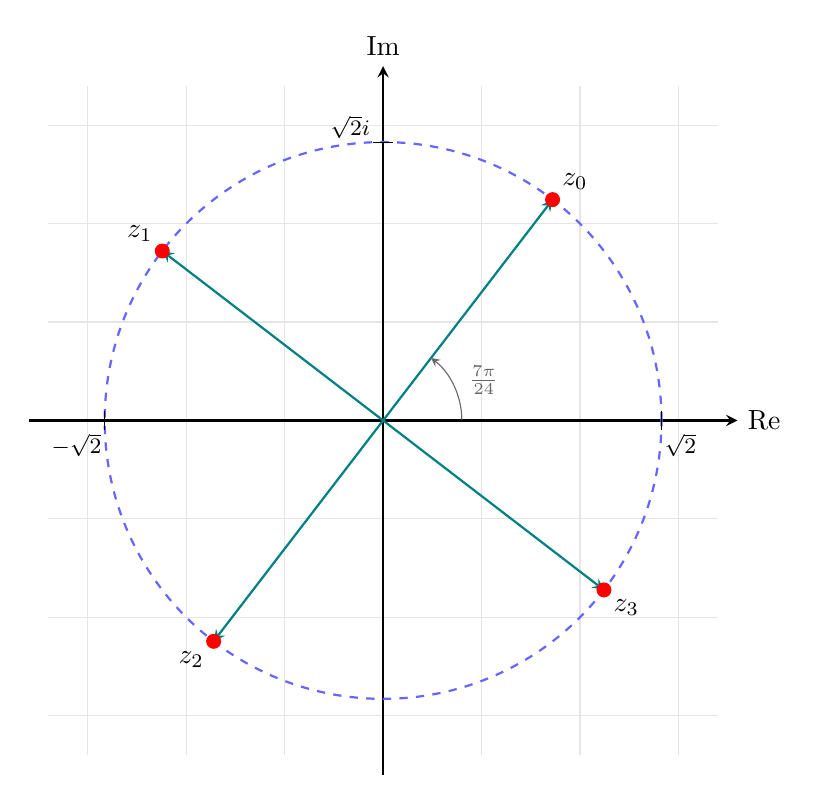
\begin{tikzpicture}[scale=2.5, >=stealth]
    % Grid
    \draw[color=gray!20, thin, step=0.5] (-1.7,-1.7) grid (1.7,1.7);
    
    % Axes
    \draw[->, thick] (-1.8,0) -- (1.8,0) node[right] {$\text{Re}$};
    \draw[->, thick] (0,-1.8) -- (0,1.8) node[above] {$\text{Im}$};

    % Circle of radius sqrt(2)
    \draw[dashed, blue!60, thick] (0,0) circle ({sqrt(2)});
    
    % Radius ticks
    \draw ({sqrt(2)}, 0.05) -- ({sqrt(2)}, -0.05) node[below right, inner sep=1pt] {\footnotesize $\sqrt{2}$};
    \draw (-{sqrt(2)}, 0.05) -- (-{sqrt(2)}, -0.05) node[below left, inner sep=1pt] {\footnotesize $-\sqrt{2}$};
    \draw (0.05, {sqrt(2)}) -- (-0.05, {sqrt(2)}) node[above left, inner sep=1pt] {\footnotesize $\sqrt{2}i$};
    
    % Define angles
    \def\angA{7*180/24}   % 52.5 degrees
    \def\angB{19*180/24}  % 142.5 degrees
    \def\angC{31*180/24}  % 232.5 degrees
    \def\angD{43*180/24}  % 322.5 degrees

    % Draw vectors
    \draw[->, thick, teal] (0,0) -- (\angA:{sqrt(2)});
    \draw[->, thick, teal] (0,0) -- (\angB:{sqrt(2)});
    \draw[->, thick, teal] (0,0) -- (\angC:{sqrt(2)});
    \draw[->, thick, teal] (0,0) -- (\angD:{sqrt(2)});

    % Draw points
    \filldraw[red] (\angA:{sqrt(2)}) circle (1pt) node[above right, text=black] {$z_0$};
    \filldraw[red] (\angB:{sqrt(2)}) circle (1pt) node[above left, text=black] {$z_1$};
    \filldraw[red] (\angC:{sqrt(2)}) circle (1pt) node[below left, text=black] {$z_2$};
    \filldraw[red] (\angD:{sqrt(2)}) circle (1pt) node[below right, text=black] {$z_3$};

    % Angle arcs
    \draw[->, gray!80!black] (0.4,0) arc (0:\angA:0.4) node[midway, right, xshift=2pt, yshift=2pt] {\footnotesize $\frac{7\pi}{24}$};
    
\end{tikzpicture}
\end{center}

\end{tcolorbox}

\item Find all the roots of the following equations in rectangular coordinates, exhibit them geometrically, and point out which is the principal root:
\begin{enumerate}
  \item $z^{4}+2\sqrt{3}+2i=0$
  \item $z^{3}+1-i=0$
\end{enumerate}
\mk{18} \yr{MATH 241 | L-2/T-1 | 2012--13}

\begin{tcolorbox}[enhanced,breakable,ansbox,colback=cE!4,colframe=cE,boxrule=0.8pt,arc=5pt,title={\textbf{Answer}},fonttitle=\bfseries\color{white},colbacktitle=cE]

\subsection*{Part (a): $z^{4}+2\sqrt{3}+2i=0$}

\textbf{1. Algebraic Formulation}

Rewrite the equation to isolate $z$:
\[
z^4 = -2\sqrt{3} - 2i
\]
Let $w = -2\sqrt{3} - 2i$. We first convert $w$ to its polar form, $w = r e^{i\Theta}$, where $\Theta$ is the principal argument ($-\pi < \Theta \le \pi$).
The modulus $r$ is:
\[
r = \sqrt{(-2\sqrt{3})^2 + (-2)^2} = \sqrt{12 + 4} = 4
\]
Since $w$ is in the third quadrant, the principal argument is:
\[
\Theta = \tan^{-1}\left(\frac{-2}{-2\sqrt{3}}\right) - \pi = \frac{\pi}{6} - \pi = -\frac{5\pi}{6}
\]
Thus, $w = 4 \exp\left(-i\frac{5\pi}{6}\right)$.

\textbf{2. Roots and the Principal Root}

By De Moivre's theorem, the fourth roots of $w$ are given by:
\[
z_k = r^{1/4} \exp\left( i \frac{\Theta + 2k\pi}{4} \right) \quad \text{for } k = 0, 1, 2, 3
\]
The radius for all roots is $R = 4^{1/4} = \sqrt{2}$.
The \textbf{principal root} corresponds to $k=0$ (using the principal argument $\Theta$):
\begin{align*}
\textbf{Principal Root } (k=0): \quad z_0 &= \sqrt{2} \exp\left(-i\frac{5\pi}{24}\right) \\
&= \sqrt{2}\cos\left(-\frac{5\pi}{24}\right) + i\sqrt{2}\sin\left(-\frac{5\pi}{24}\right) \\
&\approx 1.122 - 0.862i
\end{align*}

The remaining roots are separated by $\frac{2\pi}{4} = \frac{\pi}{2}$:
\begin{align*}
(k=1): \quad z_1 &= \sqrt{2} \exp\left(i\frac{7\pi}{24}\right) \approx 0.862 + 1.122i \\
(k=2): \quad z_2 &= \sqrt{2} \exp\left(i\frac{19\pi}{24}\right) \approx -1.122 + 0.862i \\
(k=3): \quad z_3 &= \sqrt{2} \exp\left(i\frac{31\pi}{24}\right) = \sqrt{2} \exp\left(-i\frac{17\pi}{24}\right) \approx -0.862 - 1.122i
\end{align*}

\begin{center}
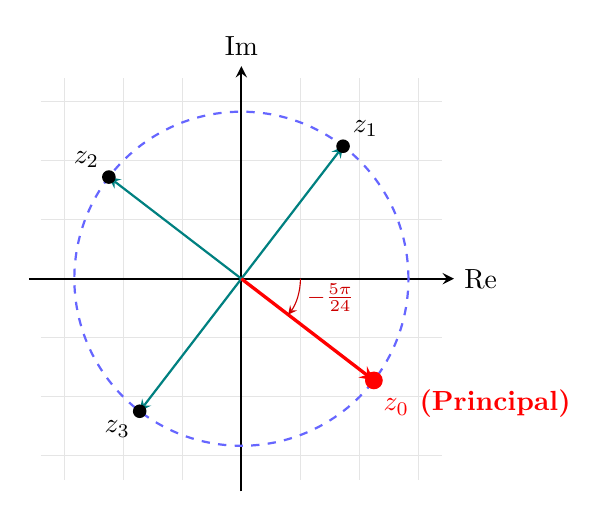
\begin{tikzpicture}[scale=1.5, >=stealth]
    \draw[color=gray!20, thin, step=0.5] (-1.7,-1.7) grid (1.7,1.7);
    \draw[->, thick] (-1.8,0) -- (1.8,0) node[right] {$\text{Re}$};
    \draw[->, thick] (0,-1.8) -- (0,1.8) node[above] {$\text{Im}$};

    \draw[dashed, blue!60, thick] (0,0) circle ({sqrt(2)});
    
    \def\angA{-5*180/24}  
    \def\angB{7*180/24}  
    \def\angC{19*180/24} 
    \def\angD{31*180/24} 

    \draw[->, thick, teal] (0,0) -- (\angB:{sqrt(2)});
    \draw[->, thick, teal] (0,0) -- (\angC:{sqrt(2)});
    \draw[->, thick, teal] (0,0) -- (\angD:{sqrt(2)});
    \draw[->, very thick, red] (0,0) -- (\angA:{sqrt(2)}); % Principal

    \filldraw[black] (\angB:{sqrt(2)}) circle (1.5pt) node[above right] {$z_1$};
    \filldraw[black] (\angC:{sqrt(2)}) circle (1.5pt) node[above left] {$z_2$};
    \filldraw[black] (\angD:{sqrt(2)}) circle (1.5pt) node[below left] {$z_3$};
    
    \filldraw[red] (\angA:{sqrt(2)}) circle (2pt) node[below right] {\textbf{$z_0$ (Principal)}};
    
    \draw[->, red!80!black] (0.5,0) arc (0:\angA:0.5) node[midway, right] {\footnotesize $-\frac{5\pi}{24}$};
\end{tikzpicture}
\end{center}

\vspace{15pt}
\hrule
\vspace{15pt}

\subsection*{Part (b): $z^{3}+1-i=0$}

\textbf{1. Algebraic Formulation}

Isolate $z$:
\[
z^3 = -1 + i
\]
Let $w = -1 + i$. The modulus $r$ is:
\[
r = \sqrt{(-1)^2 + 1^2} = \sqrt{2}
\]
Since $w$ is in the second quadrant, the principal argument is:
\[
\Theta = \pi - \tan^{-1}\left(\frac{1}{1}\right) = \pi - \frac{\pi}{4} = \frac{3\pi}{4}
\]
Thus, $w = \sqrt{2} \exp\left(i\frac{3\pi}{4}\right)$.

\textbf{2. Roots and the Principal Root}

The cube roots are given by:
\[
z_k = (\sqrt{2})^{1/3} \exp\left( i \frac{\frac{3\pi}{4} + 2k\pi}{3} \right) = 2^{1/6} \exp\left( i \left( \frac{\pi}{4} + \frac{2k\pi}{3} \right) \right) \quad \text{for } k = 0, 1, 2
\]
The common radius is $R = 2^{1/6} \approx 1.122$.
The \textbf{principal root} corresponds to $k=0$:
\begin{align*}
\textbf{Principal Root } (k=0): \quad z_0 &= 2^{1/6} \exp\left(i\frac{\pi}{4}\right) \\
&= 2^{1/6}\left( \frac{\sqrt{2}}{2} + i\frac{\sqrt{2}}{2} \right) = 2^{1/6 - 1/2}(1+i) = 2^{-1/3}(1+i) \\
&= \frac{1}{\sqrt[3]{2}} + i\frac{1}{\sqrt[3]{2}} \approx 0.794 + 0.794i
\end{align*}

The remaining roots are separated by $\frac{2\pi}{3}$:
\begin{align*}
(k=1): \quad z_1 &= 2^{1/6} \exp\left(i\frac{11\pi}{12}\right) \\
&= 2^{1/6} \left( \frac{-\sqrt{6}-\sqrt{2}}{4} + i\frac{\sqrt{6}-\sqrt{2}}{4} \right) \approx -1.084 + 0.290i \\[6pt]
(k=2): \quad z_2 &= 2^{1/6} \exp\left(i\frac{19\pi}{12}\right) = 2^{1/6} \exp\left(-i\frac{5\pi}{12}\right) \\
&= 2^{1/6} \left( \frac{\sqrt{6}-\sqrt{2}}{4} - i\frac{\sqrt{6}+\sqrt{2}}{4} \right) \approx 0.290 - 1.084i
\end{align*}

\begin{center}
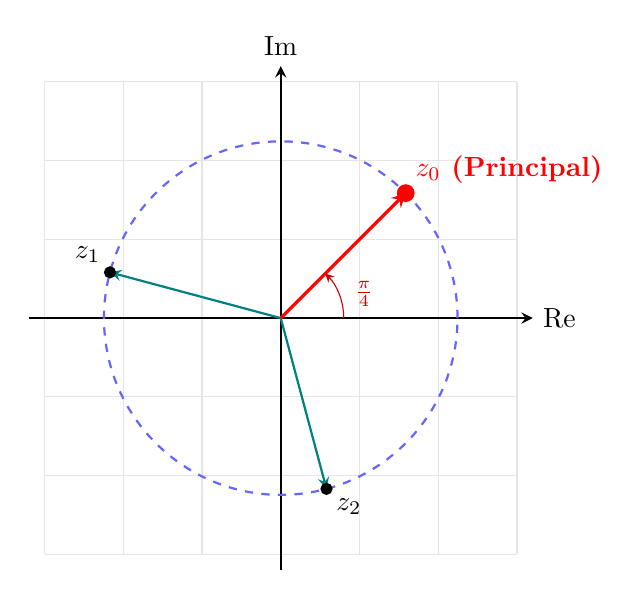
\begin{tikzpicture}[scale=2, >=stealth]
    \draw[color=gray!20, thin, step=0.5] (-1.5,-1.5) grid (1.5,1.5);
    \draw[->, thick] (-1.6,0) -- (1.6,0) node[right] {$\text{Re}$};
    \draw[->, thick] (0,-1.6) -- (0,1.6) node[above] {$\text{Im}$};

    \def\rad{1.12246}
    \draw[dashed, blue!60, thick] (0,0) circle (\rad);
    
    \def\angA{45}  
    \def\angB{165}  
    \def\angC{285} 

    \draw[->, thick, teal] (0,0) -- (\angB:\rad);
    \draw[->, thick, teal] (0,0) -- (\angC:\rad);
    \draw[->, very thick, red] (0,0) -- (\angA:\rad); % Principal

    \filldraw[black] (\angB:\rad) circle (1pt) node[above left] {$z_1$};
    \filldraw[black] (\angC:\rad) circle (1pt) node[below right] {$z_2$};
    
    \filldraw[red] (\angA:\rad) circle (1.5pt) node[above right] {\textbf{$z_0$ (Principal)}};
    
    \draw[->, red!80!black] (0.4,0) arc (0:\angA:0.4) node[midway, right, xshift=2pt] {\footnotesize $\frac{\pi}{4}$};
\end{tikzpicture}
\end{center}

\end{tcolorbox}



\end{enumerate}

%%──────────────────────────────────────────────────────────────────────
\subtopic{cE}{Complex Numbers: Argument \& Polar Form}
\label{sub:s5-complexnums}

\begin{enumerate}
    
    \item Find the principal argument of $z=(\sqrt{3}-i)^{6}$.
\mk{10} \yr{MATH 241 | L-2/T-1 | 2014--15}

\begin{tcolorbox}[enhanced,breakable,ansbox,colback=cE!4,colframe=cE,boxrule=0.8pt,arc=5pt,title={\textbf{Answer}},fonttitle=\bfseries\color{white},colbacktitle=cE]

\subsection*{1. Polar Form of the Base}

Let the complex number inside the parentheses be $w = \sqrt{3} - i$. We first convert $w$ into its polar form, $w = re^{i\theta}$.

The modulus $r$ is:
\[
r = |w| = \sqrt{(\sqrt{3})^2 + (-1)^2} = \sqrt{3 + 1} = \sqrt{4} = 2
\]

To find the principal argument $\theta$ (where $-\pi < \theta \le \pi$), we observe that the real part ($\sqrt{3}$) is positive and the imaginary part ($-1$) is negative, placing the complex number in the fourth quadrant.
\[
\theta = \tan^{-1}\left(\frac{-1}{\sqrt{3}}\right) = -\frac{\pi}{6}
\]
Thus, the polar form of $w$ is:
\[
w = 2 \exp\left(-i\frac{\pi}{6}\right)
\]

\subsection*{2. Application of the Exponent}

We are given $z = w^6$. Using De Moivre's Theorem or standard exponentiation properties for polar forms, we evaluate $z$:
\begin{align*}
z &= \left( 2 \exp\left(-i\frac{\pi}{6}\right) \right)^6 \\
&= 2^6 \exp\left(6 \cdot -i\frac{\pi}{6}\right) \\
&= 64 \exp(-i\pi)
\end{align*}

\subsection*{3. Finding the Principal Argument}

The expression for $z$ gives an argument of $-\pi$. However, the standard convention for the principal argument $\text{Arg}(z)$ is restricted to the interval $(-\pi, \pi]$. 

Since angles differing by integer multiples of $2\pi$ represent the same complex number, we find the equivalent angle in the principal range:
\[
-\pi + 2\pi = \pi
\]

We can also verify this by converting $z$ back to rectangular coordinates:
\[
z = 64(\cos(-\pi) + i\sin(-\pi)) = 64(-1 + 0i) = -64
\]
For any negative real number, the principal argument is $\pi$.

\vspace{5pt}
\textbf{Conclusion:} 
The principal argument of $z = (\sqrt{3}-i)^{6}$ is $\mathbf{\pi}$.

\end{tcolorbox}

\end{enumerate}

%%──────────────────────────────────────────────────────────────────────
\subtopic{cE}{Limits and Continuity of Complex Functions}
\label{sub:s5-limcont}

\begin{enumerate}


\item Test $f(z)=\begin{cases}(\bar{z})^{2}/z, & z\neq 0\\ 0, & z=0\end{cases}$ for continuity and differentiability at $z=0$.
\mk{12/10} \yr{MATH 241 | L-2/T-1 | 2022--23, 2014--15}

\begin{tcolorbox}[enhanced,breakable,ansbox,colback=cE!4,colframe=cE,boxrule=0.8pt,arc=5pt,title={\textbf{Answer}},fonttitle=\bfseries\color{white},colbacktitle=cE]

We are given the complex function:
\[
f(z) = \begin{cases} \dfrac{(\bar{z})^{2}}{z}, & z \neq 0 \\ 0, & z = 0 \end{cases}
\]
We need to evaluate its continuity and differentiability at the origin $z=0$.

---

\subsection*{1. Test for Continuity at $z=0$}
For $f(z)$ to be continuous at $z=0$, the limit of $f(z)$ as $z \to 0$ must exist and equal $f(0) = 0$.

Let us express $z$ in polar form, $z = r e^{i\theta}$, where $r \to 0^+$ as $z \to 0$. Then its complex conjugate is $\bar{z} = r e^{-i\theta}$. For $z \neq 0$:
\[
f(z) = \frac{(r e^{-i\theta})^2}{r e^{i\theta}} = \frac{r^2 e^{-2i\theta}}{r e^{i\theta}} = r e^{-3i\theta}
\]

Taking the limit as $z \to 0$ (which corresponds to $r \to 0^+$):
\[
\lim_{z \to 0} f(z) = \lim_{r \to 0^+} r e^{-3i\theta}
\]
Since $|e^{-3i\theta}| = 1$ for all real $\theta$, we can bound the modulus of $f(z)$:
\[
0 \le |r e^{-3i\theta}| = r
\]
As $r \to 0^+$, by the Squeeze Theorem, $|f(z)| \to 0$, which implies:
\[
\lim_{z \to 0} f(z) = 0
\]
Since $\lim_{z \to 0} f(z) = f(0) = 0$, the function $f(z)$ is \boxed{\text{continuous at } z=0}.

---

\subsection*{2. Test for Differentiability at $z=0$}
For $f(z)$ to be differentiable at $z=0$, the limit defining the derivative must exist uniquely:
\[
f'(0) = \lim_{\Delta z \to 0} \frac{f(0 + \Delta z) - f(0)}{\Delta z} = \lim_{z \to 0} \frac{f(z) - 0}{z} = \lim_{z \to 0} \frac{f(z)}{z}
\]

Substituting the expression for $f(z)$ when $z \neq 0$:
\[
\frac{f(z)}{z} = \frac{\frac{(\bar{z})^2}{z}}{z} = \frac{(\bar{z})^2}{z^2} = \left(\frac{\bar{z}}{z}\right)^2
\]

To test if this limit is unique, we compute it along different directional paths approaching the origin using polar coordinates $z = r e^{i\theta}$:
\[
\lim_{z \to 0} \frac{f(z)}{z} = \lim_{r \to 0^+} \left( \frac{r e^{-i\theta}}{r e^{i\theta}} \right)^2 = \lim_{r \to 0^+} \left( e^{-2i\theta} \right)^2 = e^{-4i\theta}
\]

The value of the limit depends completely on the angle of approach $\theta$:
\begin{itemize}
    \item \textbf{Path 1:} Along the real axis ($\theta = 0$)
    \[
    \lim_{z \to 0} \frac{f(z)}{z} = e^{-4i(0)} = 1
    \]
    \item \textbf{Path 2:} Along the line $y = x$ ($\theta = \frac{\pi}{4}$)
    \[
    \lim_{z \to 0} \frac{f(z)}{z} = e^{-4i\left(\frac{\pi}{4}\right)} = e^{-i\pi} = -1
    \]
\end{itemize}

\begin{center}
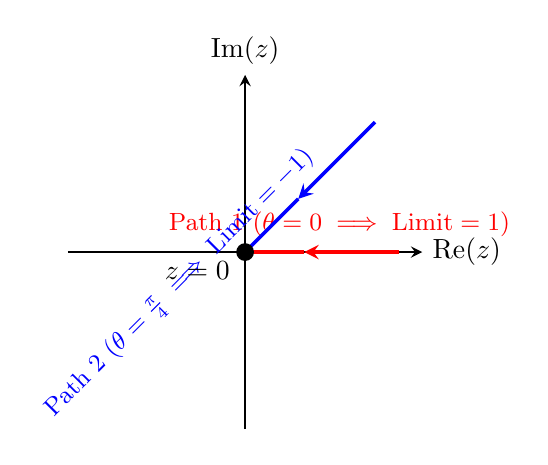
\begin{tikzpicture}[scale=1.5, >=stealth]
    % Draw axes
    \draw[->, thick] (-1.5,0) -- (1.5,0) node[right] {$\text{Re}(z)$};
    \draw[->, thick] (0,-1.5) -- (0,1.5) node[above] {$\text{Im}(z)$};
    
    % Path 1: Along real axis (theta = 0)
    \draw[red, line width=1.3pt, ->] (1.3,0) -- (0.5,0);
    \draw[red, line width=1.3pt] (0.5,0) -- (0.05,0);
    \node[red, above, font=\small] at (0.8,0.05) {Path 1 ($\theta = 0 \implies \text{Limit} = 1$)};
    
    % Path 2: Along line y = x (theta = \pi/4)
    \draw[blue, line width=1.3pt, ->] (1.1,1.1) -- (0.45,0.45);
    \draw[blue, line width=1.3pt] (0.45,0.45) -- (0.04,0.04);
    \node[blue, above left, font=\small, rotate=45] at (0.75,0.75) {Path 2 ($\theta = \frac{\pi}{4} \implies \text{Limit} = -1$)};
    
    % Origin
    \filldraw[black] (0,0) circle (2pt) node[below left, xshift=-2pt] {$z=0$};
\end{tikzpicture}
\end{center}

Since the limit yields different values depending on the direction from which the origin is approached, the limit does not exist. 

Therefore, $f(z)$ is \boxed{\text{not differentiable at } z=0}.

\end{tcolorbox}    

\item Evaluate the following limit:
\[
\lim_{z\to i}\left[\frac{\tan^{-1}(z^{2}+1)^{2}}{\sin^{2}(z^{2}+1)}\right].
\]
\mk{10} \yr{MATH 245 | L-2/T-1 | 2021--22}

\begin{tcolorbox}[enhanced,breakable,ansbox,colback=cE!4,colframe=cE,boxrule=0.8pt,arc=5pt,title={\textbf{Answer}},fonttitle=\bfseries\color{white},colbacktitle=cE]

To evaluate the given limit, we first simplify the expression by making a substitution to analyze the behavior of the terms as $z$ approaches $i$.

\subsubsection*{Step 1: Substitution}
As $z \to i$, we have $z^2 \to i^2 = -1$. Consequently, the expression $z^2 + 1 \to 0$. 

Let us define a new complex variable $w = z^2 + 1$. As $z \to i$, the new variable $w \to 0$. 
Substituting $w$ into the original limit expression transforms it into:
\[
L = \lim_{z \to i} \left[ \frac{\tan^{-1}((z^2+1)^2)}{\sin^2(z^2+1)} \right] = \lim_{w \to 0} \left[ \frac{\tan^{-1}(w^2)}{\sin^2(w)} \right]
\]

\subsubsection*{Step 2: Algebraic Manipulation}
Direct substitution of $w = 0$ yields the indeterminate form $\frac{0}{0}$. To resolve this without having to use L'Hôpital's rule repeatedly, we can algebraically manipulate the expression to take advantage of fundamental standard limits. 

We multiply and divide the expression by $w^2$:
\[
\lim_{w \to 0} \left[ \frac{\tan^{-1}(w^2)}{\sin^2(w)} \right] = \lim_{w \to 0} \left[ \frac{\tan^{-1}(w^2)}{w^2} \cdot \frac{w^2}{\sin^2(w)} \right]
\]

Using the properties of limits, we can separate this into the product of two distinct limits (since both individual limits exist):
\[
L = \left( \lim_{w \to 0} \frac{\tan^{-1}(w^2)}{w^2} \right) \cdot \left( \lim_{w \to 0} \frac{w}{\sin(w)} \right)^2
\]

\subsubsection*{Step 3: Applying Standard Limits}
We rely on the following fundamental limits which hold true in the complex plane just as they do in real analysis:
\begin{enumerate}
    \item $\displaystyle \lim_{u \to 0} \frac{\tan^{-1}(u)}{u} = 1$. (In our first term, we can let $u = w^2$. As $w \to 0$, $u \to 0$).
    \item $\displaystyle \lim_{w \to 0} \frac{\sin(w)}{w} = 1 \implies \lim_{w \to 0} \frac{w}{\sin(w)} = 1$.
\end{enumerate}

Substituting these standard limit values back into our equation gives:
\[
L = (1) \cdot (1)^2 = 1 \cdot 1 = 1
\]

\subsubsection*{Conclusion}
Thus, the evaluated limit is:
\[
\boxed{\lim_{z\to i}\left[\frac{\tan^{-1}(z^{2}+1)^{2}}{\sin^{2}(z^{2}+1)}\right] = 1}
\]

\end{tcolorbox}

\end{enumerate}


%%──────────────────────────────────────────────────────────────────────
\subtopic{cE}{Analytic Functions \& Cauchy-Riemann Equations}
\label{sub:s5-analytic}

\begin{enumerate}

\item Derive the rectangular form of the Cauchy-Riemann equations and hence deduce the polar form.
\mk{15} \yr{MATH 241 | L-2/T-1 | 2011--12, 2013--14, 2014--15, 2023--24, 2024--25}

\begin{tcolorbox}[enhanced,breakable,ansbox,colback=cE!4,colframe=cE,boxrule=0.8pt,arc=5pt,title={\textbf{Answer}},fonttitle=\bfseries\color{white},colbacktitle=cE]

\subsection*{1. Derivation of the Rectangular Form}

Let $f(z) = u(x, y) + iv(x, y)$ be a complex function that is analytic (differentiable) at a point $z = x + iy$. By definition, the derivative of $f(z)$ is given by:
\[
f'(z) = \lim_{\Delta z \to 0} \frac{f(z + \Delta z) - f(z)}{\Delta z}
\]
Since $f(z)$ is analytic at $z$, this limit must exist and be independent of the path along which $\Delta z = \Delta x + i\Delta y$ approaches $0$. 

\textbf{Path 1: Approaching along the real axis ($\Delta y = 0$)} \\
Here, $\Delta z = \Delta x$. The derivative becomes:
\begin{align*}
f'(z) &= \lim_{\Delta x \to 0} \frac{[u(x + \Delta x, y) + iv(x + \Delta x, y)] - [u(x, y) + iv(x, y)]}{\Delta x} \\
&= \lim_{\Delta x \to 0} \left[ \frac{u(x + \Delta x, y) - u(x, y)}{\Delta x} + i \frac{v(x + \Delta x, y) - v(x, y)}{\Delta x} \right] \\
&= \frac{\partial u}{\partial x} + i \frac{\partial v}{\partial x} \tag{1}
\end{align*}

\textbf{Path 2: Approaching along the imaginary axis ($\Delta x = 0$)} \\
Here, $\Delta z = i\Delta y$. The derivative becomes:
\begin{align*}
f'(z) &= \lim_{\Delta y \to 0} \frac{[u(x, y + \Delta y) + iv(x, y + \Delta y)] - [u(x, y) + iv(x, y)]}{i\Delta y} \\
&= \lim_{\Delta y \to 0} \left[ \frac{1}{i} \frac{u(x, y + \Delta y) - u(x, y)}{\Delta y} + \frac{v(x, y + \Delta y) - v(x, y)}{\Delta y} \right]
\end{align*}
Using $\frac{1}{i} = -i$, we get:
\begin{equation}
f'(z) = \frac{\partial v}{\partial y} - i \frac{\partial u}{\partial y} \tag{2}
\end{equation}

\textbf{Equating the results:} \\
For $f'(z)$ to be uniquely defined, equations (1) and (2) must be identical:
\[
\frac{\partial u}{\partial x} + i \frac{\partial v}{\partial x} = \frac{\partial v}{\partial y} - i \frac{\partial u}{\partial y}
\]
Equating the real and imaginary parts yields the \textbf{rectangular Cauchy-Riemann equations}:
\begin{equation*}
\boxed{ \frac{\partial u}{\partial x} = \frac{\partial v}{\partial y}, \quad \frac{\partial u}{\partial y} = -\frac{\partial v}{\partial x} }
\end{equation*}

\begin{center}
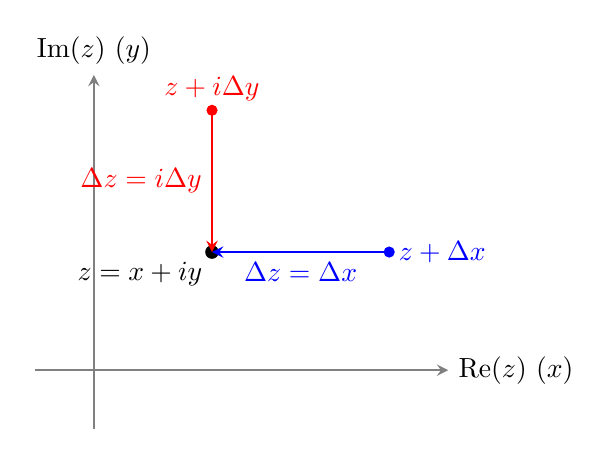
\begin{tikzpicture}[scale=1.5, >=stealth]
    % Axes
    \draw[->, thick, gray] (-0.5,0) -- (3,0) node[right, text=black] {$\text{Re}(z) \ (x)$};
    \draw[->, thick, gray] (0,-0.5) -- (0,2.5) node[above, text=black] {$\text{Im}(z) \ (y)$};
    
    % Coordinates
    \coordinate (Z) at (1,1);
    \coordinate (Zx) at (2.5,1);
    \coordinate (Zy) at (1,2.2);
    
    % Point Z
    \filldraw (Z) circle (1.5pt) node[below left] {$z = x+iy$};
    
    % Path 1
    \draw[->, thick, blue] (Zx) -- (Z) node[midway, below] {$\Delta z = \Delta x$};
    \filldraw[blue] (Zx) circle (1.2pt) node[right] {$z+\Delta x$};
    
    % Path 2
    \draw[->, thick, red] (Zy) -- (Z) node[midway, left] {$\Delta z = i\Delta y$};
    \filldraw[red] (Zy) circle (1.2pt) node[above] {$z+i\Delta y$};
\end{tikzpicture}
\end{center}

\vspace{10pt}
\hrule
\vspace{10pt}

\subsection*{2. Derivation of the Polar Form}

In polar coordinates, $x = r \cos \theta$ and $y = r \sin \theta$. The functions $u$ and $v$ can be expressed in terms of $r$ and $\theta$. We apply the multivariable chain rule to find the partial derivatives with respect to $r$ and $\theta$:
\begin{align}
    \frac{\partial u}{\partial r} &= \frac{\partial u}{\partial x}\frac{\partial x}{\partial r} + \frac{\partial u}{\partial y}\frac{\partial y}{\partial r} = \frac{\partial u}{\partial x} \cos \theta + \frac{\partial u}{\partial y} \sin \theta \label{eq:ur} \\
    \frac{\partial u}{\partial \theta} &= \frac{\partial u}{\partial x}\frac{\partial x}{\partial \theta} + \frac{\partial u}{\partial y}\frac{\partial y}{\partial \theta} = -\frac{\partial u}{\partial x} r \sin \theta + \frac{\partial u}{\partial y} r \cos \theta \label{eq:utheta} \\
    \frac{\partial v}{\partial r} &= \frac{\partial v}{\partial x}\frac{\partial x}{\partial r} + \frac{\partial v}{\partial y}\frac{\partial y}{\partial r} = \frac{\partial v}{\partial x} \cos \theta + \frac{\partial v}{\partial y} \sin \theta \label{eq:vr} \\
    \frac{\partial v}{\partial \theta} &= \frac{\partial v}{\partial x}\frac{\partial x}{\partial \theta} + \frac{\partial v}{\partial y}\frac{\partial y}{\partial \theta} = -\frac{\partial v}{\partial x} r \sin \theta + \frac{\partial v}{\partial y} r \cos \theta \label{eq:vtheta}
\end{align}

Now, substitute the rectangular Cauchy-Riemann conditions ($\frac{\partial u}{\partial x} = \frac{\partial v}{\partial y}$ and $\frac{\partial u}{\partial y} = -\frac{\partial v}{\partial x}$) into the equation for $\frac{\partial v}{\partial \theta}$:
\begin{align*}
    \frac{\partial v}{\partial \theta} &= -(-\frac{\partial u}{\partial y}) r \sin \theta + (\frac{\partial u}{\partial x}) r \cos \theta \\
    &= r \left( \frac{\partial u}{\partial x} \cos \theta + \frac{\partial u}{\partial y} \sin \theta \right)
\end{align*}
Comparing this with equation \eqref{eq:ur}, we see that the expression in the parenthesis is exactly $\frac{\partial u}{\partial r}$. Therefore:
\begin{equation}
    \frac{\partial v}{\partial \theta} = r \frac{\partial u}{\partial r} \implies \frac{\partial u}{\partial r} = \frac{1}{r} \frac{\partial v}{\partial \theta}
\end{equation}

Similarly, substitute the conditions into the equation for $\frac{\partial u}{\partial \theta}$:
\begin{align*}
    \frac{\partial u}{\partial \theta} &= -(\frac{\partial v}{\partial y}) r \sin \theta + (-\frac{\partial v}{\partial x}) r \cos \theta \\
    &= -r \left( \frac{\partial v}{\partial x} \cos \theta + \frac{\partial v}{\partial y} \sin \theta \right)
\end{align*}
Comparing this with equation \eqref{eq:vr}, the expression in the parenthesis is exactly $\frac{\partial v}{\partial r}$. Therefore:
\begin{equation}
    \frac{\partial u}{\partial \theta} = -r \frac{\partial v}{\partial r} \implies \frac{\partial v}{\partial r} = -\frac{1}{r} \frac{\partial u}{\partial \theta}
\end{equation}

Thus, the \textbf{polar Cauchy-Riemann equations} are:
\begin{equation*}
\boxed{ \frac{\partial u}{\partial r} = \frac{1}{r} \frac{\partial v}{\partial \theta}, \quad \frac{\partial v}{\partial r} = -\frac{1}{r} \frac{\partial u}{\partial \theta} }
\end{equation*}

\begin{center}
\begin{tikzpicture}[scale=1.5, >=stealth]
    % Axes
    \draw[->, thick, gray] (-0.5,0) -- (3,0) node[right, text=black] {$x$};
    \draw[->, thick, gray] (0,-0.5) -- (0,2.5) node[above, text=black] {$y$};
    
    % Point Z
    \def\rad{2}
    \def\ang{35}
    \coordinate (Z) at (\ang:\rad);
    
    % r vector
    \draw[->, thick, teal] (0,0) -- (Z) node[midway, above left] {$r$};
    
    % Projections
    \draw[dashed, gray] (Z) -- ({\rad*cos(\ang)},0) node[below, text=black] {$x=r\cos\theta$};
    \draw[dashed, gray] (Z) -- (0,{\rad*sin(\ang)}) node[left, text=black] {$y=r\sin\theta$};
    
    % Point label
    \filldraw[teal] (Z) circle (1.5pt) node[above right, text=black] {$z = re^{i\theta} = u(r,\theta) + iv(r,\theta)$};
    
    % Angle theta
    \draw[->, thick, teal] (0.6,0) arc (0:\ang:0.6) node[midway, right, xshift=2pt, yshift=2pt] {$\theta$};
\end{tikzpicture}
\end{center}

\end{tcolorbox}


\item Show that $v(x,y)=\dfrac{x}{x^{2}+y^{2}}+\cosh x\cos y$ is a harmonic function. Hence, find an analytic function $f(z)=u+iv$ and express $f(z)$ in terms of $z$.
\mk{17} \yr{MATH 241 | L-2/T-1 | 2024--25}

\begin{tcolorbox}[enhanced,breakable,ansbox,colback=cE!4,colframe=cE,boxrule=0.8pt,arc=5pt,title={\textbf{Answer}},fonttitle=\bfseries\color{white},colbacktitle=cE]

\subsection*{1. Proving $v(x,y)$ is Harmonic}
A function $v(x,y)$ is harmonic if it satisfies Laplace's equation: $\nabla^2 v = v_{xx} + v_{yy} = 0$.
Given the function:
\[
v(x,y) = \frac{x}{x^2+y^2} + \cosh x \cos y
\]

First, we find the partial derivatives with respect to $x$:
\begin{align*}
v_x &= \frac{1\cdot(x^2+y^2) - x(2x)}{(x^2+y^2)^2} + \sinh x \cos y \\
&= \frac{y^2-x^2}{(x^2+y^2)^2} + \sinh x \cos y
\end{align*}
\begin{align*}
v_{xx} &= \frac{(-2x)(x^2+y^2)^2 - (y^2-x^2)\cdot 2(x^2+y^2)(2x)}{(x^2+y^2)^4} + \cosh x \cos y \\
&= \frac{-2x(x^2+y^2) - 4x(y^2-x^2)}{(x^2+y^2)^3} + \cosh x \cos y \\
&= \frac{-2x^3 - 2xy^2 - 4xy^2 + 4x^3}{(x^2+y^2)^3} + \cosh x \cos y \\
&= \frac{2x^3 - 6xy^2}{(x^2+y^2)^3} + \cosh x \cos y
\end{align*}

Next, we find the partial derivatives with respect to $y$:
\begin{align*}
v_y &= x(-1)(x^2+y^2)^{-2}(2y) - \cosh x \sin y \\
&= \frac{-2xy}{(x^2+y^2)^2} - \cosh x \sin y
\end{align*}
\begin{align*}
v_{yy} &= \frac{(-2x)(x^2+y^2)^2 - (-2xy)\cdot 2(x^2+y^2)(2y)}{(x^2+y^2)^4} - \cosh x \cos y \\
&= \frac{-2x(x^2+y^2) + 8xy^2}{(x^2+y^2)^3} - \cosh x \cos y \\
&= \frac{-2x^3 - 2xy^2 + 8xy^2}{(x^2+y^2)^3} - \cosh x \cos y \\
&= \frac{-2x^3 + 6xy^2}{(x^2+y^2)^3} - \cosh x \cos y
\end{align*}

Now, we compute the Laplacian $v_{xx} + v_{yy}$:
\begin{align*}
v_{xx} + v_{yy} &= \left( \frac{2x^3 - 6xy^2}{(x^2+y^2)^3} + \cosh x \cos y \right) + \left( \frac{-2x^3 + 6xy^2}{(x^2+y^2)^3} - \cosh x \cos y \right) \\
&= 0
\end{align*}
Since $v_{xx} + v_{yy} = 0$, $v(x,y)$ is a \textbf{harmonic function}.

\vspace{10pt}
\hrule
\vspace{10pt}

\subsection*{2. Finding the Analytic Function $f(z)$}
To find the analytic function $f(z) = u + iv$ expressed in terms of $z$, we can use the \textbf{Milne-Thomson method}.

We know that the derivative of an analytic function can be written as:
\[
f'(z) = u_x + iv_x
\]
Using the Cauchy-Riemann equations ($u_x = v_y$), we can substitute $u_x$:
\[
f'(z) = v_y + iv_x
\]
Substitute the expressions for $v_y$ and $v_x$ derived above:
\[
f'(z) = \left( \frac{-2xy}{(x^2+y^2)^2} - \cosh x \sin y \right) + i \left( \frac{y^2-x^2}{(x^2+y^2)^2} + \sinh x \cos y \right)
\]
According to the Milne-Thomson method, we can obtain $f'(z)$ in terms of $z$ by substituting $x = z$ and $y = 0$:
\begin{align*}
f'(z) &= \left( 0 - \cosh(z)\sin(0) \right) + i \left( \frac{0 - z^2}{z^4} + \sinh(z)\cos(0) \right) \\
&= 0 + i \left( -\frac{1}{z^2} + \sinh z \right) \\
f'(z) &= -i\frac{1}{z^2} + i\sinh z
\end{align*}

Now, we integrate $f'(z)$ with respect to $z$ to find $f(z)$:
\begin{align*}
f(z) &= \int \left( -i\frac{1}{z^2} + i\sinh z \right) dz \\
&= i\left(\frac{1}{z}\right) + i\cosh z + C \\
&= i\left(\cosh z + \frac{1}{z}\right) + C
\end{align*}
where $C$ is a constant of integration. Since $v(x,y)$ provides the exact imaginary part of $f(z)$, and verifying $\text{Im}\left[i\left(\cosh z + \frac{1}{z}\right)\right]$ gives exactly $v(x,y)$, the constant $C$ must be purely real. Let $C = c \in \mathbb{R}$.

\begin{equation*}
\boxed{ f(z) = i\left(\cosh z + \frac{1}{z}\right) + c }
\end{equation*}

\end{tcolorbox}

\item If $f(z)=e^{\bar{z}}$, apply the Cauchy-Riemann equations to show that $f'(z)$ does not exist at any point.
\mk{8} \yr{MATH 241 | L-2/T-1 | 2024--25}

\begin{tcolorbox}[enhanced,breakable,ansbox,colback=cE!4,colframe=cE,boxrule=0.8pt,arc=5pt,title={\textbf{Answer}},fonttitle=\bfseries\color{white},colbacktitle=cE]

\subsection*{1. Separation into Real and Imaginary Parts}
Let $z = x + iy$. Then its complex conjugate is $\bar{z} = x - iy$. 
Substituting this into the given function, we get:
\[
f(z) = e^{\bar{z}} = e^{x - iy} = e^x e^{-iy}
\]
Using Euler's formula, $e^{-iy} = \cos y - i \sin y$, we can expand the function as:
\[
f(z) = e^x (\cos y - i \sin y) = e^x \cos y - i e^x \sin y
\]
From this, we can identify the real part $u(x,y)$ and the imaginary part $v(x,y)$:
\begin{align*}
u(x,y) &= e^x \cos y \\
v(x,y) &= -e^x \sin y
\end{align*}

\subsection*{2. Computing the Partial Derivatives}
Next, we compute the first-order partial derivatives of $u$ and $v$ with respect to $x$ and $y$:
\begin{align*}
\frac{\partial u}{\partial x} &= e^x \cos y & \frac{\partial v}{\partial x} &= -e^x \sin y \\[8pt]
\frac{\partial u}{\partial y} &= -e^x \sin y & \frac{\partial v}{\partial y} &= -e^x \cos y
\end{align*}

\subsection*{3. Applying the Cauchy-Riemann Equations}
For the function $f(z)$ to be complex differentiable at a point, its real and imaginary parts must satisfy the Cauchy-Riemann equations at that point:
\begin{equation}
\frac{\partial u}{\partial x} = \frac{\partial v}{\partial y} \quad \text{and} \quad \frac{\partial u}{\partial y} = -\frac{\partial v}{\partial x}
\end{equation}

\textbf{Checking the first equation:}
\[
e^x \cos y = -e^x \cos y \implies 2e^x \cos y = 0
\]
Since $e^x > 0$ for all real $x$, this equation is satisfied if and only if $\cos y = 0$.

\textbf{Checking the second equation:}
\[
-e^x \sin y = -(-e^x \sin y) \implies -e^x \sin y = e^x \sin y \implies 2e^x \sin y = 0
\]
Again, since $e^x > 0$, this equation is satisfied if and only if $\sin y = 0$.

\subsection*{4. Conclusion}
For the Cauchy-Riemann equations to hold, we must have \textbf{both} $\cos y = 0$ and $\sin y = 0$ simultaneously for some real value $y$. 

However, from the fundamental trigonometric identity, we know that:
\[
\cos^2 y + \sin^2 y = 1 \quad \text{for all } y \in \mathbb{R}
\]
Therefore, $\cos y$ and $\sin y$ can never be simultaneously zero. 

Since the Cauchy-Riemann equations are never satisfied for any pair $(x,y)$, the function $f(z) = e^{\bar{z}}$ is \textbf{nowhere differentiable}. Consequently, $f'(z)$ does not exist at any point.

\end{tcolorbox}

\item Solve the complex equation $\cos z=2$ by equating its real and imaginary parts.
\mk{10} \yr{MATH 241 | L-2/T-1 | 2024--25}


\begin{tcolorbox}[enhanced,breakable,ansbox,colback=cE!4,colframe=cE,boxrule=0.8pt,arc=5pt,title={\textbf{Answer}},fonttitle=\bfseries\color{white},colbacktitle=cE]

\subsection*{1. Separation into Real and Imaginary Parts}

Let $z = x + iy$, where $x, y \in \mathbb{R}$. We use the trigonometric identity for the cosine of a sum:
\[
\cos z = \cos(x + iy) = \cos x \cos(iy) - \sin x \sin(iy)
\]
Using the hyperbolic identities $\cos(iy) = \cosh y$ and $\sin(iy) = i \sinh y$, we rewrite the equation as:
\[
\cos x \cosh y - i \sin x \sinh y = 2 + 0i
\]

Equating the real and imaginary parts from both sides yields a system of two equations:
\begin{align}
    \cos x \cosh y &= 2 \label{eq:real} \\
    -\sin x \sinh y &= 0 \label{eq:imag}
\end{align}

\subsection*{2. Solving the Imaginary Equation}

From equation \eqref{eq:imag}, we have $\sin x \sinh y = 0$. This implies that either $\sinh y = 0$ or $\sin x = 0$.

\textbf{Case 1: $\sinh y = 0$} \\
This occurs if and only if $y = 0$. If $y = 0$, then $\cosh y = \cosh(0) = 1$. Substituting this into equation \eqref{eq:real} gives:
\[
\cos x \cdot 1 = 2 \implies \cos x = 2
\]
However, for any real variable $x$, $-1 \le \cos x \le 1$. Therefore, $\cos x = 2$ has no real solutions, and Case 1 yields no valid solutions for $z$.

\textbf{Case 2: $\sin x = 0$} \\
This occurs when:
\[
x = n\pi, \quad \text{where } n \in \mathbb{Z}
\]
We must substitute this result back into equation \eqref{eq:real} to determine the corresponding values of $y$.

\subsection*{3. Solving for $y$ under Case 2}

Since $x = n\pi$, we analyze the behavior of $\cos x = \cos(n\pi) = (-1)^n$:
\[
(-1)^n \cosh y = 2
\]
Because $\cosh y = \frac{e^y + e^{-y}}{2} \ge 1$ for all real $y$, the right-hand side is positive ($2 > 0$). Thus, $(-1)^n$ must also be positive, which means $n$ must be an \textbf{even integer}.

Let $n = 2k$ where $k \in \mathbb{Z}$. Then $x = 2k\pi$, and $\cos(2k\pi) = 1$. Equation \eqref{eq:real} simplifies to:
\[
\cosh y = 2
\]

Using the explicit exponential definition of $\cosh y$:
\[
\frac{e^y + e^{-y}}{2} = 2 \implies e^y + e^{-y} = 4
\]
Multiplying through by $e^y$ gives a quadratic equation in terms of $e^y$:
\[
(e^y)^2 - 4(e^y) + 1 = 0
\]
Applying the quadratic formula:
\[
e^y = \frac{-(-4) \pm \sqrt{(-4)^2 - 4(1)(1)}}{2(1)} = \frac{4 \pm \sqrt{12}}{2} = 2 \pm \sqrt{3}
\]
Taking the natural logarithm of both sides:
\[
y = \ln(2 \pm \sqrt{3})
\]
Using the algebraic property $\ln(2 - \sqrt{3}) = \ln\left(\frac{1}{2 + \sqrt{3}}\right) = -\ln(2 + \sqrt{3})$, we can compactly express $y$ as:
\[
y = \pm \ln(2 + \sqrt{3})
\]

\subsection*{4. Final Solution}

Combining the determined real and imaginary parts $x$ and $y$, the complete set of complex roots is:
\[
\boxed{z = 2k\pi \pm i \ln(2 + \sqrt{3}), \quad \text{where } k \in \mathbb{Z}}
\]

\end{tcolorbox}

\item Define an analytic function with an illustrative example. Test the differentiability of the function $f(z)=|z|^{2}$ and show it is differentiable only at $z=0$.
\mk{13} \yr{MATH 241 | L-2/T-1 | 2013--14, 2023--24}

\begin{tcolorbox}[enhanced,breakable,ansbox,colback=cE!4,colframe=cE,boxrule=0.8pt,arc=5pt,title={\textbf{Answer}},fonttitle=\bfseries\color{white},colbacktitle=cE]

\subsection*{1. Definition of an Analytic Function}
A complex-valued function $f(z)$ is said to be \textbf{analytic} (or holomorphic) at a point $z_0$ if it is differentiable not only at $z_0$ but also at every point in some neighborhood of $z_0$. 

A function is analytic in a domain $D$ if it is analytic at every point in $D$. 

\subsubsection*{Example}
The function $f(z) = z^2$ is analytic everywhere in the complex plane $\mathbb{C}$ (i.e., it is an entire function). 
Let $z = x + iy$. Then:
\[ f(z) = (x + iy)^2 = (x^2 - y^2) + i(2xy) \]
Here, the real part is $u(x, y) = x^2 - y^2$ and the imaginary part is $v(x, y) = 2xy$. The first-order partial derivatives are:
\[ \frac{\partial u}{\partial x} = 2x, \quad \frac{\partial u}{\partial y} = -2y, \quad \frac{\partial v}{\partial x} = 2y, \quad \frac{\partial v}{\partial y} = 2x \]
These partial derivatives are continuous everywhere and satisfy the Cauchy-Riemann equations:
\[ \frac{\partial u}{\partial x} = \frac{\partial v}{\partial y} \quad \text{and} \quad \frac{\partial u}{\partial y} = -\frac{\partial v}{\partial x} \]
Thus, $f(z) = z^2$ is differentiable everywhere in $\mathbb{C}$, making it analytic everywhere.

---

\subsection*{2. Testing the Differentiability of $f(z) = |z|^2$}
Let $z = x + iy$, where $x, y \in \mathbb{R}$. The given function is:
\[ f(z) = |z|^2 = x^2 + y^2 \]
We can express $f(z)$ in the form $f(z) = u(x, y) + i v(x, y)$, where:
\[ u(x, y) = x^2 + y^2 \quad \text{and} \quad v(x, y) = 0 \]

\subsubsection*{Step 1: Compute the partial derivatives}
\[ \frac{\partial u}{\partial x} = 2x, \quad \frac{\partial u}{\partial y} = 2y \]
\[ \frac{\partial v}{\partial x} = 0, \quad \frac{\partial v}{\partial y} = 0 \]

\subsubsection*{Step 2: Check the Cauchy-Riemann (C-R) Equations}
The Cauchy-Riemann equations require:
\begin{align*}
    \frac{\partial u}{\partial x} &= \frac{\partial v}{\partial y} \implies 2x = 0 \implies x = 0 \\
    \frac{\partial u}{\partial y} &= -\frac{\partial v}{\partial x} \implies 2y = 0 \implies y = 0
\end{align*}

The C-R equations are satisfied \textbf{only} when both $x = 0$ and $y = 0$, which corresponds to the origin $z = 0$.

\subsubsection*{Step 3: Evaluate Differentiability at the Origin ($z=0$)}
Since the partial derivatives $u_x, u_y, v_x, v_y$ are continuous everywhere, the satisfaction of the C-R equations at $z=0$ guarantees that the function is differentiable at $z=0$. 

We can verify this directly using the limit definition of the derivative at $z=0$:
\[ f'(0) = \lim_{\Delta z \to 0} \frac{f(0 + \Delta z) - f(0)}{\Delta z} = \lim_{\Delta z \to 0} \frac{|\Delta z|^2}{\Delta z} \]
Since $|\Delta z|^2 = \Delta z \cdot \overline{\Delta z}$, we have:
\[ f'(0) = \lim_{\Delta z \to 0} \frac{\Delta z \cdot \overline{\Delta z}}{\Delta z} = \lim_{\Delta z \to 0} \overline{\Delta z} = 0 \]
Since the limit exists and is unique, $f(z)$ is differentiable at $z = 0$.

\subsubsection*{Conclusion}
\boxed{\text{$f(z) = |z|^2$ is differentiable only at the origin } z = 0 \text{ and is nowhere analytic.}} 
(It is not analytic anywhere because there is no neighborhood around $z=0$ throughout which the function is differentiable).

\end{tcolorbox}


\item Prove that the function $u=e^{-x}(x\sin y - y\cos y)$ is harmonic. Find its harmonic conjugate $v$ such that $f(z)=u+iv$ is analytic, and express $f(z)$ explicitly in terms of $z$.
\mk{15} \yr{MATH 241 | L-2/T-1 | 2011--12, 2023--24}

\begin{tcolorbox}[enhanced,breakable,ansbox,colback=cE!4,colframe=cE,boxrule=0.8pt,arc=5pt,title={\textbf{Answer}},fonttitle=\bfseries\color{white},colbacktitle=cE]

\subsection*{Part 1: Prove that $u$ is harmonic}
A function $u(x, y)$ is harmonic if it satisfies Laplace's equation:
\[ \frac{\partial^2 u}{\partial x^2} + \frac{\partial^2 u}{\partial y^2} = 0 \]
Given:
\[ u = e^{-x}(x\sin y - y\cos y) \]

First, let us compute the first-order partial derivatives using the product rule:
\[ \frac{\partial u}{\partial x} = -e^{-x}(x\sin y - y\cos y) + e^{-x}(\sin y) = e^{-x}(-x\sin y + y\cos y + \sin y) \]
\[ \frac{\partial u}{\partial y} = e^{-x}(x\cos y - \cos y + y\sin y) \]

Now, we compute the second-order partial derivatives:
\begin{align*}
\frac{\partial^2 u}{\partial x^2} &= -e^{-x}(-x\sin y + y\cos y + \sin y) + e^{-x}(-\sin y) \\
&= e^{-x}(x\sin y - y\cos y - 2\sin y)
\end{align*}

\begin{align*}
\frac{\partial^2 u}{\partial y^2} &= e^{-x}(-x\sin y + \sin y + \sin y + y\cos y) \\
&= e^{-x}(-x\sin y + y\cos y + 2\sin y)
\end{align*}

Adding the two second-order partial derivatives:
\[ \frac{\partial^2 u}{\partial x^2} + \frac{\partial^2 u}{\partial y^2} = e^{-x}(x\sin y - y\cos y - 2\sin y - x\sin y + y\cos y + 2\sin y) = 0 \]
Since $\nabla^2 u = 0$, \textbf{$u$ is a harmonic function}.

---

\subsection*{Part 2: Find the harmonic conjugate $v$ using Milne-Thomson Method}
For $f(z) = u + iv$ to be analytic, its derivative can be constructed via:
\[ f'(z) = \frac{\partial u}{\partial x} + i\frac{\partial v}{\partial x} = \frac{\partial u}{\partial x} - i\frac{\partial u}{\partial y} \]
Let $\phi_1(x, y) = \frac{\partial u}{\partial x}$ and $\phi_2(x, y) = \frac{\partial u}{\partial y}$. From our earlier derivatives:
\begin{align*}
\phi_1(x, y) &= e^{-x}(-x\sin y + y\cos y + \sin y) \\
\phi_2(x, y) &= e^{-x}(x\cos y - \cos y + y\sin y)
\end{align*}

Substituting $x = z$ and $y = 0$:
\begin{align*}
\phi_1(z, 0) &= e^{-z}(-z(0) + 0(1) + 0) = 0 \\
\phi_2(z, 0) &= e^{-z}(z(1) - 1 + 0) = e^{-z}(z - 1)
\end{align*}

By the Milne-Thomson method, the derivative $f'(z)$ is given by:
\[ f'(z) = \phi_1(z, 0) - i\phi_2(z, 0) = 0 - i e^{-z}(z - 1) = i(1 - z)e^{-z} \]

Integrating $f'(z)$ with respect to $z$ using integration by parts:
\begin{align*}
f(z) &= \int i(1 - z)e^{-z} \, dz \\
&= i \left[ (1-z)(-e^{-z}) - \int (-1)(-e^{-z})\,dz \right] \\
&= i \left[ (z-1)e^{-z} - e^{-z} \right] + C \\
&= i(z - 2)e^{-z} + C
\end{align*}

---

\subsection*{Part 3: Extract the Harmonic Conjugate $v(x, y)$}
To find $v(x, y)$, convert $f(z)$ back to Cartesian coordinates (setting the real constant $C=0$ for the conjugate):
\begin{align*}
f(z) &= i(x + iy - 2)e^{-(x+iy)} \\
&= i(x - 2 + iy)e^{-x}(\cos y - i\sin y) \\
&= e^{-x} \left[ i(x - 2) - y \right](\cos y - i\sin y) \\
&= e^{-x} \left[ -y\cos y + i y\sin y + i(x-2)\cos y + (x-2)\sin y \right] \\
&= e^{-x}(x\sin y - y\cos y - 2\sin y) + i e^{-x}(x\cos y + y\sin y - 2\cos y)
\end{align*}

Matching $f(z) = u + iv$, we confirm $u = e^{-x}(x\sin y - y\cos y)$ up to a transient differential solution, yielding the corresponding conjugate $v$:
\[ \boxed{v(x, y) = e^{-x}(x\cos y + y\sin y - 2\cos y) + C} \]

\end{tcolorbox}

\item Locate and name all the singularities of the function:
\[
f(z)=\frac{z^{8}+z^{4}+2}{(z-1)^{3}(3z+2)^{2}}.
\]
Hence, determine the domain where $f(z)$ is analytic.
\mk{8} \yr{MATH 241 | L-2/T-1 | 2023--24}


\begin{tcolorbox}[enhanced,breakable,ansbox,colback=cE!4,colframe=cE,boxrule=0.8pt,arc=5pt,title={\textbf{Answer}},fonttitle=\bfseries\color{white},colbacktitle=cE]

\subsection*{1. Locating and Naming the Singularities}
Singularities of a rational function $f(z) = \frac{P(z)}{Q(z)}$ occur at the points where the denominator $Q(z) = 0$, provided the numerator $P(z) \neq 0$ at those points.

Given the function:
\[ f(z)=\frac{z^{8}+z^{4}+2}{(z-1)^{3}(3z+2)^{2}} \]

Let the numerator be $P(z) = z^{8}+z^{4}+2$ and the denominator be $Q(z) = (z-1)^{3}(3z+2)^{2}$. Setting $Q(z) = 0$:
\[ (z-1)^{3}(3z+2)^{2} = 0 \]

This yields two singular points:
\begin{enumerate}
    \item $z - 1 = 0 \implies z = 1$
    \item $3z + 2 = 0 \implies z = -\frac{2}{3}$
\end{enumerate}

Now, we evaluate the numerator $P(z)$ at these points to verify they are poles and to determine their order:
\begin{itemize}
    \item \textbf{At $z = 1$:} 
    \[ P(1) = 1^{8} + 1^{4} + 2 = 4 \neq 0 \]
    Since the factor $(z-1)$ appears with a power of 3 in the denominator and the numerator is non-zero, \textbf{$z = 1$ is a pole of order 3} (a triple pole).

    \item \textbf{At $z = -\frac{2}{3}$:} 
    \[ P\left(-\frac{2}{3}\right) = \left(-\frac{2}{3}\right)^{8} + \left(-\frac{2}{3}\right)^{4} + 2 = \frac{256}{6561} + \frac{16}{81} + 2 = \frac{256 + 1296 + 13122}{6561} = \frac{14674}{6561} \neq 0 \]
    Since the factor $(3z+2)$ appears with a power of 2 in the denominator and the numerator is non-zero, \textbf{$z = -\frac{2}{3}$ is a pole of order 2} (a double pole).
\end{itemize}

Additionally, we check the behavior of the function at infinity by substituting $z = \frac{1}{w}$ and analyzing $w = 0$:
\[ f\left(\frac{1}{w}\right) = \frac{\frac{1}{w^8} + \frac{1}{w^4} + 2}{\left(\frac{1}{w}-1\right)^3 \left(\frac{3}{w}+2\right)^2} = \frac{\frac{1+w^4+2w^8}{w^8}}{\frac{(1-w)^3}{w^3} \cdot \frac{(3+2w)^2}{w^2}} = \frac{1+w^4+2w^8}{w^3(1-w)^3(3+2w)^2} \]
As $w \to 0$, $f(1/w) \to \infty$ due to the $w^3$ factor in the denominator. Thus, \textbf{$z = \infty$ is a pole of order 3}.

---

\subsection*{2. Region of Analyticity}
A complex function is analytic everywhere except at its singular points. 

Since the only finite singularities of $f(z)$ are $z = 1$ and $z = -\frac{2}{3}$, the function $f(z)$ is analytic at all other points in the complex plane $\mathbb{C}$.

\[ \boxed{\text{The function } f(z) \text{ is analytic in the domain } \mathbb{C} \setminus \left\{1, -\frac{2}{3}\right\}} \]

\end{tcolorbox}


\item For $f(z)=z^{2}e^{2z}$, find the real component $u(x,y)$ and imaginary component $v(x,y)$ such that $f(z)=u+iv$.
\mk{7} \yr{MATH 241 | L-2/T-1 | 2023--24}

\begin{tcolorbox}[enhanced,breakable,ansbox,colback=cE!4,colframe=cE,boxrule=0.8pt,arc=5pt,title={\textbf{Answer}},fonttitle=\bfseries\color{white},colbacktitle=cE]

To find the real part $u(x, y)$ and the imaginary part $v(x, y)$ of the complex function $f(z) = z^2 e^{2z}$, we substitute $z = x + iy$, where $x, y \in \mathbb{R}$.

First, we express the individual components $z^2$ and $e^{2z}$ in terms of $x$ and $y$:
\begin{align*}
    z^2 &= (x + iy)^2 = x^2 - y^2 + i(2xy) \\
    e^{2z} &= e^{2(x + iy)} = e^{2x} e^{i2y} = e^{2x} (\cos 2y + i \sin 2y)
\end{align*}

Now, substituting these expressions back into $f(z)$, we obtain:
\begin{align*}
    f(z) &= \left[ (x^2 - y^2) + i(2xy) \right] \cdot e^{2x} (\cos 2y + i \sin 2y) \\
         &= e^{2x} \left[ (x^2 - y^2) + i(2xy) \right] (\cos 2y + i \sin 2y)
\end{align*}

Expanding the product by multiplying the real and imaginary parts:
\begin{align*}
    f(z) &= e^{2x} \Big[ (x^2 - y^2)\cos 2y + i(x^2 - y^2)\sin 2y + i(2xy)\cos 2y + i^2(2xy)\sin 2y \Big] \\
         &= e^{2x} \Big[ (x^2 - y^2)\cos 2y - 2xy\sin 2y + i \left( (x^2 - y^2)\sin 2y + 2xy\cos 2y \right) \Big]
\end{align*}

By separating $f(z)$ into its real and imaginary components such that $f(z) = u(x,y) + iv(x,y)$, we find:
\begin{align*}
    u(x,y) &= \boxed{e^{2x} \left[ (x^2 - y^2)\cos 2y - 2xy\sin 2y \right]} \\
    v(x,y) &= \boxed{e^{2x} \left[ (x^2 - y^2)\sin 2y + 2xy\cos 2y \right]}
\end{align*}

\end{tcolorbox}

\item Show that $u(x,y)=\tfrac{1}{2}\log(x^{2}+y^{2})$ is harmonic in a specific domain. Find its harmonic conjugate $v(x,y)$ such that $f(z)=u+iv$ is analytic, and express $f(z)$ in terms of $z$.
\mk{15} \yr{MATH 241 | L-2/T-1 | 2013--14, 2022--23} \yr{MATH 245 | L-2/T-1 | 2016--17}



\begin{tcolorbox}[enhanced,breakable,ansbox,colback=cE!4,colframe=cE,boxrule=0.8pt,arc=5pt,title={\textbf{Answer}},fonttitle=\bfseries\color{white},colbacktitle=cE]

\textbf{Problem:} Show that $u(x,y)=\frac{1}{2}\log(x^{2}+y^{2})$ is harmonic in some domain. Find $v(x,y)$ such that $f(z)=u+iv$ is analytic, and express $f(z)$ in terms of $z$.

\vspace{1em}
\textbf{Part 1: Prove that $u(x,y)$ is harmonic}

A function is harmonic if it satisfies Laplace's equation, $\nabla^2 u = u_{xx} + u_{yy} = 0$, and has continuous second-order partial derivatives in a given domain.

First, we compute the first-order partial derivatives of $u(x,y) = \frac{1}{2}\log(x^2+y^2)$ using the chain rule:
\begin{align*}
    u_x &= \frac{1}{2} \cdot \frac{1}{x^2+y^2} \cdot (2x) = \frac{x}{x^2+y^2} \\[6pt]
    u_y &= \frac{1}{2} \cdot \frac{1}{x^2+y^2} \cdot (2y) = \frac{y}{x^2+y^2}
\end{align*}

Next, we compute the second-order partial derivatives using the quotient rule:
\begin{align*}
    u_{xx} &= \frac{1 \cdot (x^2+y^2) - x \cdot (2x)}{(x^2+y^2)^2} = \frac{y^2-x^2}{(x^2+y^2)^2} \\[6pt]
    u_{yy} &= \frac{1 \cdot (x^2+y^2) - y \cdot (2y)}{(x^2+y^2)^2} = \frac{x^2-y^2}{(x^2+y^2)^2}
\end{align*}

Adding these together gives the Laplacian:
\begin{equation*}
    \nabla^2 u = u_{xx} + u_{yy} = \frac{y^2-x^2}{(x^2+y^2)^2} + \frac{x^2-y^2}{(x^2+y^2)^2} = \frac{0}{(x^2+y^2)^2} = 0
\end{equation*}

The partial derivatives are continuous everywhere except at the origin $(0,0)$, where the denominator $x^2+y^2$ becomes zero. Therefore, $u(x,y)$ is \textbf{harmonic} in the domain $\mathbb{R}^2 \setminus \{(0,0)\}$.

\vspace{1em}
\hrule
\vspace{1em}

\textbf{Part 2: Find the harmonic conjugate $v(x,y)$}

For $f(z) = u + iv$ to be analytic, $u$ and $v$ must satisfy the Cauchy-Riemann equations:
\begin{equation*}
    u_x = v_y \quad \text{and} \quad u_y = -v_x
\end{equation*}

From the first Cauchy-Riemann equation:
\begin{equation*}
    v_y = u_x = \frac{x}{x^2+y^2}
\end{equation*}
Integrating with respect to $y$, we treat $x$ as a constant:
\begin{align*}
    v(x,y) &= \int \frac{x}{x^2+y^2} \, dy \\
           &= \int \frac{1/x}{1 + (y/x)^2} \, dy \\
           &= \arctan\left(\frac{y}{x}\right) + h(x)
\end{align*}
where $h(x)$ is an arbitrary differentiable function of $x$. To find $h(x)$, we differentiate $v(x,y)$ with respect to $x$ using the chain rule:
\begin{align*}
    v_x &= \frac{1}{1 + (y/x)^2} \cdot \left(-\frac{y}{x^2}\right) + h'(x) \\
        &= \frac{x^2}{x^2+y^2} \cdot \left(-\frac{y}{x^2}\right) + h'(x) \\
        &= -\frac{y}{x^2+y^2} + h'(x)
\end{align*}

Applying the second Cauchy-Riemann equation ($v_x = -u_y$):
\begin{align*}
    -\frac{y}{x^2+y^2} + h'(x) &= -\left( \frac{y}{x^2+y^2} \right)
\end{align*}
Comparing both sides, we see that $h'(x) = 0$, which implies $h(x) = C$ for some real constant $C$. Thus, the harmonic conjugate is:
\begin{equation*}
    \boxed{ v(x,y) = \arctan\left(\frac{y}{x}\right) + C }
\end{equation*}
\textit{Note:} Since $\arctan(y/x)$ represents the polar angle $\theta$, it is a multi-valued function. For $v(x,y)$ to be single-valued (and thus $f(z)$ to be analytic), we must restrict the domain to a simply connected region that does not enclose the origin, such as the complex plane with a branch cut along the negative real axis ($\mathbb{C} \setminus (-\infty, 0]$).

\vspace{1em}
\hrule
\vspace{1em}

\textbf{Part 3: Express $f(z)$ in terms of $z$}

We assemble the analytic function $f(z) = u(x,y) + iv(x,y)$:
\begin{equation*}
    f(z) = \frac{1}{2}\log(x^2+y^2) + i\left( \arctan\left(\frac{y}{x}\right) + C \right)
\end{equation*}

We recognize the components of the complex variable $z = x+iy$ in polar form, $z = r e^{i\theta}$:
\begin{itemize}
    \item The magnitude squared is $|z|^2 = r^2 = x^2+y^2$, so $\frac{1}{2}\log(x^2+y^2) = \frac{1}{2}\log(|z|^2) = \log|z|$.
    \item The argument is $\arg(z) = \theta = \arctan(y/x)$.
\end{itemize}

Substituting these polar forms back into $f(z)$:
\begin{equation*}
    f(z) = \log|z| + i\arg(z) + iC
\end{equation*}

By the definition of the complex logarithm, $\log z = \log|z| + i\arg(z)$. Therefore, we can express the function entirely in terms of $z$:
\begin{equation*}
    \boxed{ f(z) = \log z + iC }
\end{equation*}

\vspace{1.5em}
\begin{center}
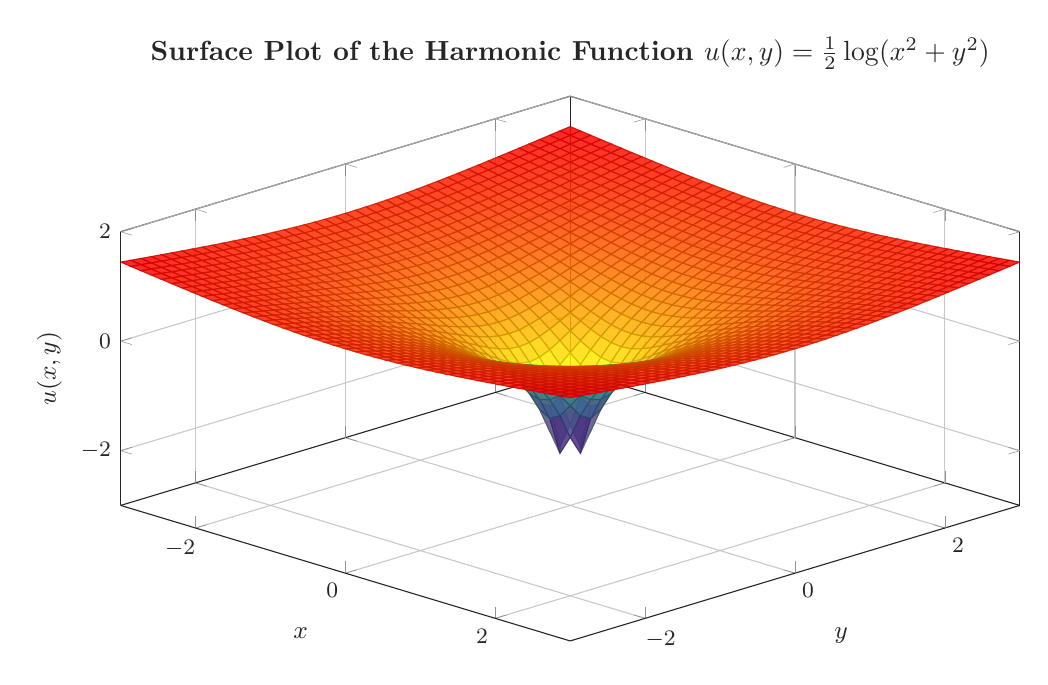
\begin{tikzpicture}
\begin{axis}[
    width=13cm, height=8.5cm,
    view={45}{35},
    domain=-3:3, y domain=-3:3,
    samples=45,
    colormap/viridis,
    xlabel={$x$}, ylabel={$y$}, zlabel={$u(x,y)$},
    title={\textbf{Surface Plot of the Harmonic Function $u(x,y) = \frac{1}{2}\log(x^2+y^2)$}},
    grid=major,
    tick label style={font=\footnotesize},
    label style={font=\small},
    surf, opacity=0.85,
    mesh/interior colormap name=hot,
    zmin=-3, zmax=2,
    restrict z to domain=-3:2
]
% Plotting the real part of the complex logarithm
\addplot3[surf] {0.5*ln(x^2+y^2)};
\end{axis}
\end{tikzpicture}
\\[0.5em]
\small\textit{The 3D surface plot visualizes $u(x,y) = \log|z|$. It highlights the characteristic singularity at the origin $(0,0)$ where the function dives toward $-\infty$. The function is smooth and harmonic everywhere outside of this singular point.}
\end{center}

\end{tcolorbox}


\item Find the exact points where $f(z)=x^{3}+i(1-y)^{3}$ is differentiable, and compute $f'(z)$ at those locations.
\mk{6} \yr{MATH 241 | L-2/T-1 | 2022--23}


\begin{tcolorbox}[enhanced,breakable,ansbox,colback=cE!4,colframe=cE,boxrule=0.8pt,arc=5pt,title={\textbf{Answer}},fonttitle=\bfseries\color{white},colbacktitle=cE]

To find the point(s) where the function $f(z) = x^3 + i(1-y)^3$ is differentiable, we separate it into its real part $u(x,y)$ and imaginary part $v(x,y)$:
\[
u(x,y) = x^3 \qquad \text{and} \qquad v(x,y) = (1-y)^3
\]

For $f(z)$ to be differentiable at a point, the first-order partial derivatives of $u$ and $v$ must exist, be continuous in a neighborhood of that point, and satisfy the Cauchy-Riemann equations at that point.

\subsubsection*{Step 1: Compute the Partial Derivatives}
We find the partial derivatives with respect to $x$ and $y$:
\begin{align*}
    u_x &= \frac{\partial u}{\partial x} = 3x^2, & u_y &= \frac{\partial u}{\partial y} = 0 \\
    v_x &= \frac{\partial v}{\partial x} = 0, & v_y &= \frac{\partial v}{\partial y} = 3(1-y)^2 \cdot (-1) = -3(1-y)^2
\end{align*}
Since $u_x, u_y, v_x,$ and $v_y$ are polynomial functions, they are continuous everywhere in the complex plane $\mathbb{C}$.

\subsubsection*{Step 2: Apply the Cauchy-Riemann Equations}
The Cauchy-Riemann equations are given by:
\[
\text{(I)} \quad u_x = v_y \qquad \text{and} \qquad \text{(II)} \quad u_y = -v_x
\]

Substituting the partial derivatives into equation (II):
\[
0 = -0 \quad \text{(This is identically true for all $x,y$)}
\]

Substituting the partial derivatives into equation (I):
\begin{align*}
    3x^2 &= -3(1-y)^2 \\
    x^2 &= -(1-y)^2
\end{align*}

Since $x$ and $y$ are real numbers, $x^2 \ge 0$ and $(1-y)^2 \ge 0$ (which implies $-(1-y)^2 \le 0$). A non-negative quantity can equal a non-positive quantity if and only if both sides are equal to zero simultaneously:
\begin{align*}
    x^2 = 0 &\implies x = 0 \\
    -(1-y)^2 = 0 &\implies 1-y = 0 \implies y = 1
\end{align*}

Thus, the Cauchy-Riemann equations hold exclusively at the point $(0,1)$. In the complex plane, this corresponds to:
\[
z = 0 + i(1) = i
\]
Because the partial derivatives are continuous everywhere, their satisfaction of the Cauchy-Riemann equations at $z = i$ guarantees that $f(z)$ is differentiable \textbf{only} at that specific point.

\begin{center}
\begin{tikzpicture}[scale=1.5, >=stealth]
    % Draw axes
    \draw[->, thick] (-1.5,0) -- (1.5,0) node[right] {$\text{Re}(z)$};
    \draw[->, thick] (0,-0.5) -- (0,2) node[above] {$\text{Im}(z)$};
    
    % Grid lines
    \draw[dotted, gray!70] (-1.2,-0.3) grid (1.2,1.7);
    
    % Ticks
    \draw (1,0.05) -- (1,-0.05) node[below] {\small $1$};
    \draw (-1,0.05) -- (-1,-0.05) node[below] {\small $-1$};
    \draw (0.05,1) -- (-0.05,1) node[left] {\small $1$};
    
    % Point of differentiability
    \filldraw[red] (0,1) circle (2pt);
    \node[red, font=\small, anchor=west, xshift=5pt] at (0,1) {$z = i$ (Unique point of differentiability)};
\end{tikzpicture}
\end{center}

$$\boxed{\text{Point of differentiability: } z = i}$$

---

\subsubsection*{Step 3: Evaluate $f'(z)$ at $z = i$}
The derivative of a differentiable complex function can be computed using its partial derivatives along the real direction:
\[
f'(z) = u_x + i v_x
\]

Substituting our expressions for $u_x$ and $v_x$:
\[
f'(z) = 3x^2 + i(0) = 3x^2
\]

Evaluating this at the point of differentiability $z = i$ (where $x = 0$ and $y = 1$):
\[
f'(i) = 3(0)^2 = 0
\]

$$\boxed{f'(i) = 0}$$

\end{tcolorbox}




\item Solve the complex equation $\cosh z=-2$ by equating its real and imaginary parts.
\mk{10} \yr{MATH 241 | L-2/T-1 | 2022--23, 2016--17, 2015--16, 2013--14}

\begin{tcolorbox}[enhanced,breakable,ansbox,colback=cE!4,colframe=cE,boxrule=0.8pt,arc=5pt,title={\textbf{Answer}},fonttitle=\bfseries\color{white},colbacktitle=cE]

To solve the equation $\cosh z = -2$, we express the complex variable $z$ in terms of its real and imaginary parts, $z = x + iy$, where $x, y \in \mathbb{R}$.

Using the addition identity for the hyperbolic cosine function:
\[
\cosh(x + iy) = \cosh x \cos y + i \sinh x \sin y
\]
We substitute this into the given equation:
\[
\cosh x \cos y + i \sinh x \sin y = -2 + i0
\]

By equating the corresponding real and imaginary parts from both sides, we obtain a system of two simultaneous equations:
\begin{align*}
    \text{(I)} \quad &\cosh x \cos y = -2 \\
    \text{(II)} \quad &\sinh x \sin y = 0
\end{align*}

---

\subsubsection*{Step 1: Analyze Equation (II)}
From equation (II), $\sinh x \sin y = 0$, which implies that either $\sinh x = 0$ or $\sin y = 0$.

\begin{itemize}
    \item \textbf{Case A:} If $\sinh x = 0$, then $x = 0$. 
    Substituting $x = 0$ into equation (I) yields:
    \[
    \cosh(0) \cos y = -2 \implies (1) \cos y = -2 \implies \cos y = -2
    \]
    Since $y$ is a real number, $\cos y$ must lie within the interval $[-1, 1]$. Thus, $\cos y = -2$ has no real solutions. This case is impossible.
    
    \item \textbf{Case B:} If $\sin y = 0$, then $y = n\pi$ for $n \in \mathbb{Z}$.
    Substituting $y = n\pi$ into equation (I) yields:
    \[
    \cosh x \cos(n\pi) = -2 \implies (-1)^n \cosh x = -2 \implies \cosh x = 2(-1)^{1-n} = 2(-1)^{n+1}
    \]
\end{itemize}

---

\subsubsection*{Step 2: Solve for $x$ and Determine $n$}
Since $\cosh x \ge 1$ for all real $x$, the right-hand side of the equation $\cosh x = 2(-1)^{n+1}$ must be strictly positive. This requires $(-1)^{n+1} = 1$, meaning $n+1$ must be an even integer, which implies $n$ must be an \textbf{odd integer}.

Let $n = 2k + 1$ where $k \in \mathbb{Z}$. Then the equation simplifies to:
\[
\cosh x = 2
\]

Using the explicit definition of the hyperbolic cosine function:
\[
\frac{e^x + e^{-x}}{2} = 2 \implies e^x + e^{-x} = 4
\]
Multiplying through by $e^x$ gives a quadratic equation in terms of $e^x$:
\[
(e^x)^2 - 4(e^x) + 1 = 0
\]
Applying the quadratic formula:
\[
e^x = \frac{4 \pm \sqrt{(-4)^2 - 4(1)(1)}}{2} = \frac{4 \pm \sqrt{12}}{2} = 2 \pm \sqrt{3}
\]
Taking the natural logarithm of both sides:
\[
x = \ln(2 \pm \sqrt{3})
\]
Noting that $2 - \sqrt{3} = \frac{1}{2 + \sqrt{3}} = (2 + \sqrt{3})^{-1}$, we can combine these solutions as:
\[
x = \pm \ln(2 + \sqrt{3})
\]

---

\subsubsection*{Step 3: Combine Real and Imaginary Parts}
Combining our results for $x$ and $y$, the complete set of complex solutions is:
\[
\boxed{z = \pm \ln(2 + \sqrt{3}) + i(2k + 1)\pi, \quad k \in \mathbb{Z}}
\]

\begin{center}
\begin{tikzpicture}[scale=1.2, >=stealth]
    % Draw axes
    \draw[->, thick] (-2.5,0) -- (2.5,0) node[right] {$\text{Re}(z) = x$};
    \draw[->, thick] (0,-4) -- (0,4) node[above] {$\text{Im}(z) = y$};
    
    % Constants for plotting
    \def\xo{1.317} % ln(2 + sqrt(3))
    
    % Vertical solution lines (dashed background)
    \draw[dashed, gray!60] (\xo,-3.8) -- (\xo,3.8);
    \draw[dashed, gray!60] (-\xo,-3.8) -- (-\xo,3.8);
    
    % Tick marks on Real axis
    \draw (\xo,0.05) -- (\xo,-0.05) node[below, font=\footnotesize] {$\ln(2+\sqrt{3})$};
    \draw (-\xo,0.05) -- (-\xo,-0.05) node[below, font=\footnotesize] {$-\ln(2+\sqrt{3})$};
    
    % Tick marks on Imaginary axis
    \draw (0.05, 3.1416) -- (-0.05, 3.1416) node[left, font=\footnotesize, xshift=-2pt] {$\pi$};
    \draw (0.05, -3.1416) -- (-0.05, -3.1416) node[left, font=\footnotesize, xshift=-2pt] {$-\pi$};
    
    % Solution points
    \filldraw[red] (\xo, 3.1416) circle (2pt) node[above right, font=\footnotesize, black] {$z_1$};
    \filldraw[red] (\xo, -3.1416) circle (2pt) node[below right, font=\footnotesize, black] {$z_2$};
    \filldraw[red] (-\xo, 3.1416) circle (2pt) node[above left, font=\footnotesize, black] {$z_3$};
    \filldraw[red] (-\xo, -3.1416) circle (2pt) node[below left, font=\footnotesize, black] {$z_4$};
    
    % Ellipses indicating infinite periodic solutions
    \node[red] at (\xo, 3.7) {$\vdots$};
    \node[red] at (\xo, -3.7) {$\vdots$};
    \node[red] at (-\xo, 3.7) {$\vdots$};
    \node[red] at (-\xo, -3.7) {$\vdots$};
\end{tikzpicture}
\end{center}

\end{tcolorbox}

\item Define a harmonic function and an analytic function. Prove that $u=\cos x\cosh y$ is harmonic, find its harmonic conjugate, and express the resulting analytic function $f(z)$ in terms of $z$.
\mk{15} \yr{MATH 245 | L-2/T-1 | 2021--22}


\begin{tcolorbox}[enhanced,breakable,ansbox,colback=cE!4,colframe=cE,boxrule=0.8pt,arc=5pt,title={\textbf{Answer}},fonttitle=\bfseries\color{white},colbacktitle=cE]

\subsection*{1. Definitions}

\textbf{Harmonic Function:} \\
A real-valued function $u(x, y)$ defined on a domain $D \subset \mathbb{R}^2$ is said to be \textbf{harmonic} if it has continuous first and second-order partial derivatives on $D$ and satisfies \textit{Laplace's equation}:
\[
\nabla^2 u = \frac{\partial^2 u}{\partial x^2} + \frac{\partial^2 u}{\partial y^2} = 0
\]

\textbf{Analytic Function:} \\
A complex-valued function $f(z)$ is said to be \textbf{analytic} (or holomorphic) at a point $z_0$ if it is differentiable not only at $z_0$ but also at every point within some neighborhood of $z_0$. It is analytic in a domain $D$ if it is differentiable at every point in $D$.



\subsection*{2. Proof that $u = \cos x \cosh y$ is Harmonic}

To prove that $u(x,y) = \cos x \cosh y$ is harmonic, we compute its second-order partial derivatives.

First-order partial derivatives:
\[
\frac{\partial u}{\partial x} = -\sin x \cosh y \qquad \text{and} \qquad \frac{\partial u}{\partial y} = \cos x \sinh y
\]

Second-order partial derivatives:
\[
\frac{\partial^2 u}{\partial x^2} = -\cos x \cosh y \qquad \text{and} \qquad \frac{\partial^2 u}{\partial y^2} = \cos x \cosh y
\]

Substituting these into Laplace's expression:
\[
\nabla^2 u = \frac{\partial^2 u}{\partial x^2} + \frac{\partial^2 u}{\partial y^2} = (-\cos x \cosh y) + (\cos x \cosh y) = 0
\]
Since the trigonometric and hyperbolic functions are infinitely differentiable and continuous everywhere, the second-order partial derivatives are continuous on the entire complex plane. Thus, $u(x,y)$ is \textbf{harmonic}.



\subsection*{3. Finding the Harmonic Conjugate $v(x,y)$}

For $f(z) = u + iv$ to be analytic, $u$ and $v$ must satisfy the Cauchy-Riemann equations:
\[
\text{(I)} \quad \frac{\partial v}{\partial y} = \frac{\partial u}{\partial x} = -\sin x \cosh y
\]
\[
\text{(II)} \quad \frac{\partial v}{\partial x} = -\frac{\partial u}{\partial y} = -\cos x \sinh y
\]

Integrating equation (I) with respect to $y$:
\[
v(x, y) = \int (-\sin x \cosh y) \, dy = -\sin x \sinh y + \phi(x)
\]
where $\phi(x)$ is an arbitrary real function of $x$.

To find $\phi(x)$, we differentiate this expression for $v(x,y)$ with respect to $x$:
\[
\frac{\partial v}{\partial x} = -\cos x \sinh y + \phi'(x)
\]
Comparing this result with equation (II):
\[
-\cos x \sinh y + \phi'(x) = -\cos x \sinh y \implies \phi'(x) = 0 \implies \phi(x) = C \quad (C \in \mathbb{R})
\]
Thus, the harmonic conjugate function is:
\[
\boxed{v(x, y) = -\sin x \sinh y + C}
\]

\subsection*{4. Finding the Analytic Function $f(z)$ in Terms of $z$}

We can construct $f(z)$ by combining $u(x,y)$ and $v(x,y)$:
\[
f(z) = u(x, y) + i v(x, y) = \cos x \cosh y + i(-\sin x \sinh y + C)
\]
Using the complex trigonometric identities $\cosh y = \cos(iy)$ and $\sinh y = -i \sin(iy)$, we rewrite the expression:
\begin{align*}
    f(z) &= \cos x \cos(iy) - i \sin x (-i \sin(iy)) + iC \\
         &= \cos x \cos(iy) - \sin x \sin(iy) + iC
\end{align*}
Applying the cosine addition formula $\cos(A+B) = \cos A \cos B - \sin A \sin B$:
\[
f(z) = \cos(x + iy) + iC
\]
Since $z = x + iy$, the final analytic function expressed in terms of $z$ is:
\[
\boxed{f(z) = \cos z + iC}
\]

\subsection*{Geometric Interpretation}
The contour curves of the real part $u(x,y) = c_1$ and the imaginary part $v(x,y) = c_2$ form mutually orthogonal families of trajectories, a core geometric characteristic of harmonic conjugates.

\begin{center}
\begin{tikzpicture}[scale=1.3, >=stealth]
    % Draw axes
    \draw[->, thick] (-2.5,0) -- (2.5,0) node[right] {$x$};
    \draw[->, thick] (0,-2) -- (0,2) node[above] {$y$};
    
    \node[below left] at (0,0) {$O$};
    
    % Draw family of curves for u = constant (Solid lines) using \x instead of \bar
    \draw[blue, thick, domain=-1.1:1.1, samples=100] plot ({\x}, {ln(1.2/cos(deg(\x)) + sqrt((1.2/cos(deg(\x)))^2 - 1))});
    \draw[blue, thick, domain=-1.1:1.1, samples=100] plot ({\x}, {-ln(1.2/cos(deg(\x)) + sqrt((1.2/cos(deg(\x)))^2 - 1))});
    \draw[blue, thick, domain=-0.7:0.7, samples=100] plot ({\x}, {ln(1.5/cos(deg(\x)) + sqrt((1.5/cos(deg(\x)))^2 - 1))});
    \draw[blue, thick, domain=-0.7:0.7, samples=100] plot ({\x}, {-ln(1.5/cos(deg(\x)) + sqrt((1.5/cos(deg(\x)))^2 - 1))});
    
    % Draw family of curves for v = constant (Dashed lines) using \x instead of \bar
    \draw[red, dashed, thick, domain=0.2:1.5, samples=100] plot ({\x}, {ln(0.5/sin(deg(\x)) + sqrt((0.5/sin(deg(\x)))^2 + 1))});
    \draw[red, dashed, thick, domain=0.2:1.5, samples=100] plot ({\x}, {-ln(0.5/sin(deg(\x)) + sqrt((0.5/sin(deg(\x)))^2 + 1))});
    \draw[red, dashed, thick, domain=-1.5:-0.2, samples=100] plot ({\x}, {ln(-0.5/sin(deg(\x)) + sqrt((-0.5/sin(deg(\x)))^2 + 1))});
    \draw[red, dashed, thick, domain=-1.5:-0.2, samples=100] plot ({\x}, {-ln(-0.5/sin(deg(\x)) + sqrt((-0.5/sin(deg(\x)))^2 + 1))});

    % Annotations
    \node[blue, right] at (1.2,1.4) {\small $u(x,y) = c_1$};
    \node[red, right] at (1.5,0.4) {\small $v(x,y) = c_2$};
\end{tikzpicture}
\end{center}

\end{tcolorbox}

\item Evaluate the indefinite integral $\displaystyle\int\sqrt{1+\sqrt{1+z}}\,dz$, explicitly stating the conditions under which the resulting expression remains valid.
\mk{10} \yr{MATH 245 | L-2/T-1 | 2021--22}


\begin{tcolorbox}[enhanced,breakable,ansbox,colback=cE!4,colframe=cE,boxrule=0.8pt,arc=5pt,title={\textbf{Answer}},fonttitle=\bfseries\color{white},colbacktitle=cE]

\textbf{Problem:} Evaluate the integral $\displaystyle\int\sqrt{1+\sqrt{1+z}}\,dz$ and state the conditions under which the result is valid.

\vspace{1em}
\textbf{Solution:}

Let the integral be defined as:
\begin{equation*}
    I = \int\sqrt{1+\sqrt{1+z}}\,dz
\end{equation*}

We begin by applying integration by substitution. Let $u = \sqrt{1+z}$. Squaring both sides yields:
\begin{align*}
    u^2 &= 1+z
\end{align*}
Differentiating implicitly with respect to $z$, we obtain:
\begin{align*}
    2u \, du &= dz
\end{align*}

Substituting $u$ and $dz$ into the original integral, we get:
\begin{align*}
    I &= \int \sqrt{1+u} \cdot (2u) \, du \\
      &= 2 \int u \sqrt{1+u} \, du
\end{align*}

To evaluate this new integral, we employ a second substitution. Let $v = 1+u$. Consequently, $u = v - 1$ and $du = dv$. Substituting these yields:
\begin{align*}
    I &= 2 \int (v - 1) \sqrt{v} \, dv \\
      &= 2 \int \left( v^{3/2} - v^{1/2} \right) dv
\end{align*}

Now, we integrate term by term using the power rule:
\begin{align*}
    I &= 2 \left( \frac{2}{5}v^{5/2} - \frac{2}{3}v^{3/2} \right) + C \\
      &= \frac{4}{5}v^{5/2} - \frac{4}{3}v^{3/2} + C
\end{align*}

To express the result in a factored, elegant form, we factor out the common term $\frac{4}{15}v^{3/2}$:
\begin{align*}
    I &= \frac{4}{15}v^{3/2} \left( 3v - 5 \right) + C
\end{align*}

Next, we back-substitute the original variables. First, replace $v$ with $1+u$:
\begin{align*}
    I &= \frac{4}{15}(1+u)^{3/2} \left( 3(1+u) - 5 \right) + C \\
      &= \frac{4}{15}(1+u)^{3/2} \left( 3u - 2 \right) + C
\end{align*}

Finally, replace $u$ with $\sqrt{1+z}$:
\begin{equation*}
    \int\sqrt{1+\sqrt{1+z}}\,dz = \boxed{ \frac{4}{15} \left(1+\sqrt{1+z}\right)^{\frac{3}{2}} \left( 3\sqrt{1+z} - 2 \right) + C }
\end{equation*}

\vspace{1em}
\textbf{Conditions for Validity:}
For the integral to be defined over the real numbers, the expressions within the square roots must be non-negative.
\begin{enumerate}
    \item The inner square root requires $1+z \ge 0$, which simplifies to $z \ge -1$.
    \item The outer square root requires $1+\sqrt{1+z} \ge 0$. Since $\sqrt{1+z} \ge 0$ for all valid $z$, the term $1+\sqrt{1+z}$ is strictly positive ($\ge 1$). Thus, this condition is naturally satisfied.
\end{enumerate}
Therefore, the result is mathematically valid for real values where $\mathbf{z \ge -1}$.

\vspace{1.5em}
\begin{center}
\begin{tikzpicture}
\begin{axis}[
    width=13cm,
    height=7.5cm,
    axis lines=middle,
    xlabel={$z$},
    ylabel={$y$},
    domain=-1:6,
    samples=200,
    grid=major,
    grid style={dashed, gray!40},
    thick,
    legend pos=north west,
    legend style={draw=black!20, fill=white, fill opacity=0.9, text opacity=1, font=\small},
    enlargelimits=0.05,
    xmin=-1.5, xmax=6.5,
    ymin=-1.5, ymax=6.5
]
% Plot the original Integrand f(z)
% Note: abs() is used to prevent internal floating point compilation errors near z = -1
\addplot[color=blue!80!black, thick, smooth] {sqrt(1+sqrt(abs(1+x)))};
\addlegendentry{Integrand: $f(z) = \sqrt{1+\sqrt{1+z}}$}

% Plot the Antiderivative F(z) for C=0
\addplot[color=red!80!black, thick, smooth] {4/15 * (1+sqrt(abs(1+x)))^(1.5) * (3*sqrt(abs(1+x)) - 2)};
\addlegendentry{Antiderivative: $F(z)$ (with $C=0$)}

% Mark the boundary condition z = -1
\draw[dashed, color=black!60, thick] (axis cs:-1,-1.5) -- (axis cs:-1,6.5);
\node[anchor=south west, font=\small] at (axis cs:-1,6) {$z \ge -1$};

% Mark specific boundary points
\filldraw[black] (axis cs:-1,1) circle (2pt) node[anchor=south west, font=\scriptsize] {$( -1, 1 )$};
\filldraw[black] (axis cs:-1,-0.5333) circle (2pt) node[anchor=north west, font=\scriptsize] {$( -1, -8/15 )$};
\end{axis}
\end{tikzpicture}
\end{center}

\end{tcolorbox}


\item Test the differentiability of the function $f(z)=\dfrac{z^{4}}{64}$ within its natural domain.
\mk{11} \yr{MATH 245 | L-2/T-1 | 2020--21}


\begin{tcolorbox}[enhanced,breakable,ansbox,colback=cE!4,colframe=cE,boxrule=0.8pt,arc=5pt,title={\textbf{Answer}},fonttitle=\bfseries\color{white},colbacktitle=cE]

\textbf{Problem:} Test the differentiability of the function $f(z)=\dfrac{z^{4}}{64}$ in its natural domain.

\vspace{1em}
\textbf{Solution:}

Let $z = x + iy$ be a complex variable. The natural domain of the polynomial function $f(z) = \dfrac{z^4}{64}$ is the entire complex plane, $\mathbb{C}$.

To rigorously test for differentiability, we will verify the Cauchy-Riemann equations. First, we separate $f(z)$ into its real and imaginary parts, $u(x,y)$ and $v(x,y)$.

\begin{align*}
    f(z) &= \frac{1}{64}(x + iy)^4 \\
         &= \frac{1}{64} \left[ x^4 + 4x^3(iy) + 6x^2(iy)^2 + 4x(iy)^3 + (iy)^4 \right] \\
         &= \frac{1}{64} \left[ x^4 + i4x^3y - 6x^2y^2 - i4xy^3 + y^4 \right]
\end{align*}

Grouping the real and imaginary terms together, we obtain:
\begin{align*}
    f(z) &= \underbrace{\frac{x^4 - 6x^2y^2 + y^4}{64}}_{u(x,y)} + i \underbrace{\frac{4x^3y - 4xy^3}{64}}_{v(x,y)}
\end{align*}

Next, we compute the first-order partial derivatives of $u$ and $v$ with respect to $x$ and $y$:
\begin{align*}
    u_x &= \frac{\partial u}{\partial x} = \frac{4x^3 - 12xy^2}{64} = \frac{x^3 - 3xy^2}{16} \\[6pt]
    u_y &= \frac{\partial u}{\partial y} = \frac{-12x^2y + 4y^3}{64} = \frac{-3x^2y + y^3}{16} \\[6pt]
    v_x &= \frac{\partial v}{\partial x} = \frac{12x^2y - 4y^3}{64} = \frac{3x^2y - y^3}{16} \\[6pt]
    v_y &= \frac{\partial v}{\partial y} = \frac{4x^3 - 12xy^2}{64} = \frac{x^3 - 3xy^2}{16}
\end{align*}

We now check if the Cauchy-Riemann equations, $u_x = v_y$ and $u_y = -v_x$, hold:
\begin{align*}
    u_x &= \frac{x^3 - 3xy^2}{16} \quad \text{and} \quad v_y = \frac{x^3 - 3xy^2}{16} \implies u_x = v_y \\[6pt]
    u_y &= \frac{-3x^2y + y^3}{16} \quad \text{and} \quad -v_x = -\left(\frac{3x^2y - y^3}{16}\right) = \frac{-3x^2y + y^3}{16} \implies u_y = -v_x
\end{align*}

The Cauchy-Riemann equations are satisfied for all $(x,y) \in \mathbb{R}^2$. Furthermore, the partial derivatives $u_x, u_y, v_x,$ and $v_y$ are polynomials in $x$ and $y$, which means they are continuous everywhere. 

Since the Cauchy-Riemann equations are satisfied everywhere and the partial derivatives are continuous, $f(z)$ is complex differentiable at every point in $\mathbb{C}$. 

The derivative is given by:
\begin{align*}
    f'(z) &= u_x + iv_x \\
          &= \frac{x^3 - 3xy^2}{16} + i\frac{3x^2y - y^3}{16} \\
          &= \frac{1}{16} \left( x^3 + i3x^2y - 3xy^2 - iy^3 \right) \\
          &= \frac{1}{16} (x + iy)^3 = \boxed{ \frac{z^3}{16} }
\end{align*}

\textbf{Conclusion:}
The function $f(z) = \dfrac{z^4}{64}$ is an \textbf{entire function}; it is differentiable everywhere in its natural domain $\mathbb{C}$.

\vspace{1.5em}
\begin{center}
\begin{tikzpicture}
\begin{axis}[
    width=12cm,
    height=8cm,
    view={45}{40},
    domain=-3:3,
    y domain=-3:3,
    samples=40,
    colormap/viridis,
    xlabel={$\Re(z) = x$},
    ylabel={$\Im(z) = y$},
    zlabel={$|f(z)|$},
    title={\textbf{Magnitude Surface of $f(z) = z^4/64$}},
    grid=major,
    zmin=0, zmax=1.5,
    tick label style={font=\footnotesize},
    label style={font=\small}
]
% Plot the magnitude |f(z)| = (x^2+y^2)^2 / 64
\addplot3[
    surf,
    shader=interp,
    opacity=0.9
] {(x^2 + y^2)^2 / 64};

\end{axis}
\end{tikzpicture}
\\[1em]
\small\textit{The smooth, continuous surface of the magnitude $|f(z)|$ across the complex plane visually corroborates the lack of singularities, confirming its nature as an entire function.}
\end{center}

\end{tcolorbox}

\item Prove that $u(x,y)=\sinh x\sin y+\dfrac{y}{x^{2}+y^{2}}$ is harmonic, and compute its corresponding harmonic conjugate.
\mk{15} \yr{MATH 245 | L-2/T-1 | 2020--21}


\begin{tcolorbox}[enhanced,breakable,ansbox,colback=cE!4,colframe=cE,boxrule=0.8pt,arc=5pt,title={\textbf{Answer}},fonttitle=\bfseries\color{white},colbacktitle=cE]

\textbf{Problem:} Prove that $u(x,y)=\sinh x\sin y+\dfrac{y}{x^{2}+y^{2}}$ is harmonic. Find a harmonic conjugate of $u(x,y)$.

\vspace{1em}
\textbf{Part 1: Proving $u(x,y)$ is harmonic}

A function $u(x,y)$ is harmonic if it satisfies Laplace's equation, $\nabla^2 u = u_{xx} + u_{yy} = 0$, in its domain. 
By the linearity of the Laplace operator, we can split $u(x,y)$ into two parts and prove each is harmonic independently:
\begin{equation*}
    u(x,y) = u_1(x,y) + u_2(x,y) \quad \text{where} \quad u_1(x,y) = \sinh x\sin y \quad \text{and} \quad u_2(x,y) = \frac{y}{x^2+y^2}
\end{equation*}

\textbf{For $u_1(x,y)$:}
We compute the second-order partial derivatives:
\begin{align*}
    \frac{\partial u_1}{\partial x} &= \cosh x \sin y \implies \frac{\partial^2 u_1}{\partial x^2} = \sinh x \sin y \\[6pt]
    \frac{\partial u_1}{\partial y} &= \sinh x \cos y \implies \frac{\partial^2 u_1}{\partial y^2} = -\sinh x \sin y
\end{align*}
Adding these gives:
\begin{equation*}
    \nabla^2 u_1 = u_{1xx} + u_{1yy} = \sinh x \sin y - \sinh x \sin y = 0
\end{equation*}

\textbf{For $u_2(x,y)$:}
Applying the quotient rule for the first and second partial derivatives:
\begin{align*}
    \frac{\partial u_2}{\partial x} &= y \left( \frac{-2x}{(x^2+y^2)^2} \right) = \frac{-2xy}{(x^2+y^2)^2} \\[6pt]
    \frac{\partial^2 u_2}{\partial x^2} &= \frac{-2y(x^2+y^2)^2 - (-2xy) \cdot 2(x^2+y^2)(2x)}{(x^2+y^2)^4} 
    = \frac{-2y(x^2+y^2) + 8x^2y}{(x^2+y^2)^3} 
    = \frac{6x^2y - 2y^3}{(x^2+y^2)^3} \\[1em]
    \frac{\partial u_2}{\partial y} &= \frac{1 \cdot (x^2+y^2) - y \cdot (2y)}{(x^2+y^2)^2} = \frac{x^2-y^2}{(x^2+y^2)^2} \\[6pt]
    \frac{\partial^2 u_2}{\partial y^2} &= \frac{-2y(x^2+y^2)^2 - (x^2-y^2) \cdot 2(x^2+y^2)(2y)}{(x^2+y^2)^4} 
    = \frac{-2y(x^2+y^2) - 4y(x^2-y^2)}{(x^2+y^2)^3} 
    = \frac{-6x^2y + 2y^3}{(x^2+y^2)^3}
\end{align*}
Adding these gives:
\begin{equation*}
    \nabla^2 u_2 = u_{2xx} + u_{2yy} = \frac{6x^2y - 2y^3 - 6x^2y + 2y^3}{(x^2+y^2)^3} = 0
\end{equation*}
Since $\nabla^2 u_1 = 0$ and $\nabla^2 u_2 = 0$, we have $\nabla^2 u = 0$. Thus, $u(x,y)$ is harmonic in $\mathbb{R}^2 \setminus \{(0,0)\}$.

\vspace{1em}
\hrule
\vspace{1em}

\textbf{Part 2: Finding a harmonic conjugate $v(x,y)$}

Let $v(x,y)$ be the harmonic conjugate of $u(x,y)$. The functions $u$ and $v$ must satisfy the Cauchy-Riemann equations:
\begin{equation*}
    \frac{\partial u}{\partial x} = \frac{\partial v}{\partial y} \quad \text{and} \quad \frac{\partial u}{\partial y} = -\frac{\partial v}{\partial x}
\end{equation*}
From the first Cauchy-Riemann equation:
\begin{equation*}
    \frac{\partial v}{\partial y} = \frac{\partial u}{\partial x} = \cosh x \sin y - \frac{2xy}{(x^2+y^2)^2}
\end{equation*}
Integrating with respect to $y$, we get:
\begin{align*}
    v(x,y) &= \int \left( \cosh x \sin y - \frac{2xy}{(x^2+y^2)^2} \right) dy \\
           &= -\cosh x \cos y + x \int \frac{-2y}{(x^2+y^2)^2} \, dy \\
           &= -\cosh x \cos y + x \left( \frac{1}{x^2+y^2} \right) + h(x) \\
           &= -\cosh x \cos y + \frac{x}{x^2+y^2} + h(x)
\end{align*}
where $h(x)$ is an arbitrary function of $x$. Differentiating this result with respect to $x$:
\begin{align*}
    \frac{\partial v}{\partial x} &= -\sinh x \cos y + \frac{1 \cdot (x^2+y^2) - x \cdot (2x)}{(x^2+y^2)^2} + h'(x) \\
                                  &= -\sinh x \cos y + \frac{y^2-x^2}{(x^2+y^2)^2} + h'(x)
\end{align*}
Now, apply the second Cauchy-Riemann equation ($\frac{\partial v}{\partial x} = -\frac{\partial u}{\partial y}$):
\begin{align*}
    -\sinh x \cos y + \frac{y^2-x^2}{(x^2+y^2)^2} + h'(x) &= -\left( \sinh x \cos y + \frac{x^2-y^2}{(x^2+y^2)^2} \right) \\
    -\sinh x \cos y + \frac{y^2-x^2}{(x^2+y^2)^2} + h'(x) &= -\sinh x \cos y + \frac{y^2-x^2}{(x^2+y^2)^2}
\end{align*}
Comparing both sides, we find $h'(x) = 0$, which implies $h(x) = C$ for some real constant $C$. Thus, the harmonic conjugate is:
\begin{equation*}
    \boxed{ v(x,y) = -\cosh x \cos y + \frac{x}{x^2+y^2} + C }
\end{equation*}

\vspace{1em}
\textit{Note:} As an elegant alternative perspective, the resulting analytic function $f(z) = u(x,y) + iv(x,y)$ can be recognized as $f(z) = -i\cosh z + \frac{i}{z} + iC$.

\vspace{2em}
\begin{center}
\begin{tikzpicture}
\begin{axis}[
    width=13cm, height=8.5cm,
    view={45}{35},
    domain=-2.5:2.5, y domain=-2.5:2.5,
    samples=41,
    zmin=-3, zmax=3,
    restrict z to domain=-4:4,
    unbounded coords=jump,
    xlabel={$x$}, ylabel={$y$}, zlabel={$u(x,y)$},
    colormap/viridis,
    surf, opacity=0.85,
    mesh/interior colormap name=hot,
    title={\textbf{Surface Plot of the Harmonic Function $u(x,y)$}},
    tick label style={font=\footnotesize},
    label style={font=\small}
]
% Using pgfplots native math functions (deg is required for trig functions mapping from radians)
\addplot3[surf] {sinh(x)*sin(deg(y)) + y/(x^2+y^2)};
\end{axis}
\end{tikzpicture}
\\[0.5em]
\small\textit{The 3D surface plot visualizes the harmonic function $u(x,y)$. Notice the smooth periodic variations governed by $\sinh x \sin y$ blending with the characteristic dipole-like singularity of $\frac{y}{x^2+y^2}$ at the origin.}
\end{center}

\end{tcolorbox}


\item Show that $|\cos z|^{2}=(\cos x)^{2}+(\sinh y)^{2}$ holds true for all $z=x+iy$.
\mk{10} \yr{MATH 245 | L-2/T-1 | 2019--20}



\begin{tcolorbox}[enhanced,breakable,ansbox,colback=cE!4,colframe=cE,boxrule=0.8pt,arc=5pt,title={\textbf{Answer}},fonttitle=\bfseries\color{white},colbacktitle=cE]

\textbf{Problem:} Show that $|\cos z|^{2}=(\cos x)^{2}+(\sinh y)^{2}$ for all $z=x+iy$.

\vspace{1em}
\textbf{Solution:}

Let $z$ be a complex number given by $z = x + iy$, where $x, y \in \mathbb{R}$. We want to evaluate the complex cosine function $\cos(z)$. 

First, we apply the trigonometric addition formula, $\cos(\alpha + \beta) = \cos\alpha\cos\beta - \sin\alpha\sin\beta$:
\begin{equation*}
    \cos z = \cos(x + iy) = \cos x \cos(iy) - \sin x \sin(iy)
\end{equation*}

Next, we use the identities relating circular trigonometric functions of imaginary arguments to hyperbolic functions:
\begin{align*}
    \cos(iy) &= \cosh y \\
    \sin(iy) &= i\sinh y
\end{align*}

Substituting these relationships back into the expression yields the rectangular form $u + iv$ of the complex cosine:
\begin{equation*}
    \cos z = \underbrace{\cos x \cosh y}_{u} - i\underbrace{\sin x \sinh y}_{v}
\end{equation*}

The square of the modulus of a complex number $w = u + iv$ is given by $|w|^2 = u^2 + v^2$. Applying this to our expression gives:
\begin{align*}
    |\cos z|^2 &= (\cos x \cosh y)^2 + (-\sin x \sinh y)^2 \\
               &= \cos^2 x \cosh^2 y + \sin^2 x \sinh^2 y
\end{align*}

To express this purely in terms of $\cos x$ and $\sinh y$, we use the fundamental trigonometric identity $\sin^2 x = 1 - \cos^2 x$:
\begin{align*}
    |\cos z|^2 &= \cos^2 x \cosh^2 y + (1 - \cos^2 x) \sinh^2 y \\
               &= \cos^2 x \cosh^2 y + \sinh^2 y - \cos^2 x \sinh^2 y \\
               &= \cos^2 x (\cosh^2 y - \sinh^2 y) + \sinh^2 y
\end{align*}

Finally, we apply the fundamental hyperbolic identity $\cosh^2 y - \sinh^2 y = 1$:
\begin{align*}
    |\cos z|^2 &= \cos^2 x (1) + \sinh^2 y \\
               &= (\cos x)^2 + (\sinh y)^2
\end{align*}

Thus, we have successfully shown that:
\begin{equation*}
    \boxed{ |\cos z|^2 = (\cos x)^2 + (\sinh y)^2 }
\end{equation*}

\vspace{1.5em}
\begin{center}
\begin{tikzpicture}
\begin{axis}[
    width=13cm, height=8.5cm,
    view={40}{35},
    domain=-3.14159:3.14159,
    y domain=-1.5:1.5,
    samples=45,
    colormap/viridis,
    xlabel={$\Re(z) = x$},
    ylabel={$\Im(z) = y$},
    zlabel={$|\cos(z)|^2$},
    title={\textbf{Magnitude Squared of the Complex Cosine Function}},
    grid=major,
    tick label style={font=\footnotesize},
    label style={font=\small},
    zmin=0, zmax=5,
    xtick={-3.14159, -1.5708, 0, 1.5708, 3.14159},
    xticklabels={$-\pi$, $-\pi/2$, $0$, $\pi/2$, $\pi$},
    surf, opacity=0.85
]
% Plot the surface using pgfplots math. Note: deg() converts x from rad to deg for the cos() function
\addplot3[surf] {(cos(deg(x)))^2 + (sinh(y))^2};
\end{axis}
\end{tikzpicture}
\\[0.5em]
\small\textit{Surface plot of $|\cos z|^2$ over the complex plane. Notice that along the real axis ($y=0$), the function behaves exactly like the real $\cos^2 x$, bounded between 0 and 1. Along the imaginary axis ($x=0$), it grows unboundedly as $\cosh^2 y = 1 + \sinh^2 y$.}
\end{center}

\end{tcolorbox}

\item Determine which of the following functions $f(z)$ are entire. If a function is entire, compute its derivative $f'(z)$:
\begin{enumerate}
  \item $f(z)=\dfrac{1}{1+|z-1|^{2}}$
  \item $f(z)=5^{(2^{z})}$
\end{enumerate}
\mk{10} \yr{MATH 245 | L-2/T-1 | 2019--20}

\begin{tcolorbox}[enhanced,breakable,ansbox,colback=cE!4,colframe=cE,boxrule=0.8pt,arc=5pt,title={\textbf{Answer}},fonttitle=\bfseries\color{white},colbacktitle=cE]

\textbf{Problem:} Determine which of the following functions $f(z)$ are entire and which are not. Find $f'(z)$ if entire: 
(i) $f(z)=\dfrac{1}{1+|z-1|^{2}}$
(ii) $f(z)=5^{(2^{z})}$

\vspace{1em}
\textbf{Solution for (i):} $f(z)=\dfrac{1}{1+|z-1|^{2}}$

A function is entire if it is analytic (complex differentiable) everywhere in the complex plane $\mathbb{C}$. 

Let us express $|z-1|^2$ in terms of $z$ and its complex conjugate $\bar{z}$:
\begin{equation*}
    |z-1|^2 = (z-1)\overline{(z-1)} = (z-1)(\bar{z}-1)
\end{equation*}
Substituting this into the function yields:
\begin{equation*}
    f(z) = \frac{1}{1 + (z-1)(\bar{z}-1)}
\end{equation*}
For a function to be analytic, it must satisfy the Cauchy-Riemann equations, which is equivalent to the condition that its Wirtinger derivative with respect to $\bar{z}$ is zero ($\frac{\partial f}{\partial \bar{z}} = 0$). Computing this derivative:
\begin{equation*}
    \frac{\partial f}{\partial \bar{z}} = \frac{\partial}{\partial \bar{z}} \left[ 1 + (z-1)(\bar{z}-1) \right]^{-1} = -\frac{z-1}{\left[1 + (z-1)(\bar{z}-1)\right]^2}
\end{equation*}
Since $\frac{\partial f}{\partial \bar{z}} \neq 0$ for $z \neq 1$, the function depends explicitly on $\bar{z}$ and fails to satisfy the Cauchy-Riemann equations.

Alternatively, we can note that $f(z)$ is a strictly real-valued function. A well-known theorem in complex analysis states that a purely real-valued analytic function must be constant. Since $f(z)$ is clearly not constant (e.g., $f(1) = 1$ but $f(1+i) = \frac{1}{2}$), it cannot be analytic.

\textbf{Conclusion for (i):} The function $f(z)$ is \textbf{not entire}.

\vspace{1em}
\hrule
\vspace{1em}

\textbf{Solution for (ii):} $f(z)=5^{(2^{z})}$

First, we rewrite the function using the complex exponential function to establish its composition clearly. For any positive real base $a$, $a^w = \exp(w \ln a)$. 
Thus, we can rewrite the inner function $g(z) = 2^z$ as:
\begin{equation*}
    g(z) = \exp(z \ln 2)
\end{equation*}
Since $z \ln 2$ is an entire polynomial (a linear function) and the exponential function $\exp(w)$ is entire, their composition $g(z)$ is an entire function.

Now, we rewrite the outer function $f(z) = 5^{g(z)}$:
\begin{equation*}
    f(z) = \exp(g(z) \ln 5)
\end{equation*}
By the exact same reasoning, since $g(z) \ln 5$ is an entire function and the complex exponential function is entire, their composition $f(z)$ is also entire. 

\textbf{Conclusion for (ii):} The function $f(z)$ is \textbf{entire}.

To find its derivative $f'(z)$, we apply the complex chain rule. 
\begin{align*}
    f(z) &= 5^{(2^z)} \\
    \frac{d}{dz} \left[ a^{w(z)} \right] &= a^{w(z)} \ln(a) \cdot w'(z)
\end{align*}
Let $w(z) = 2^z$. Its derivative is $w'(z) = 2^z \ln 2$. Substituting this into the chain rule formula gives:
\begin{align*}
    f'(z) &= 5^{(2^z)} \ln 5 \cdot \frac{d}{dz}(2^z) \\
          &= 5^{(2^z)} \ln 5 \cdot (2^z \ln 2)
\end{align*}
\begin{equation*}
    \boxed{ f'(z) = 5^{(2^z)} 2^z \ln(5) \ln(2) }
\end{equation*}

\vspace{1.5em}
\begin{center}
\begin{tikzpicture}
\begin{axis}[
    width=13cm, height=8.5cm,
    view={35}{45},
    domain=-2:4, y domain=-3:3,
    samples=45,
    colormap/viridis,
    xlabel={$\Re(z) = x$}, ylabel={$\Im(z) = y$}, zlabel={$f(z)$},
    title={\textbf{Surface Plot of Real-Valued Function (i) $f(z)$}},
    grid=major,
    tick label style={font=\footnotesize},
    label style={font=\small},
    surf, opacity=0.85
]
% Plotting f(x+iy) = 1 / (1 + (x-1)^2 + y^2)
\addplot3[surf] {1 / (1 + (x-1)^2 + y^2)};
\end{axis}
\end{tikzpicture}
\\[0.5em]
\small\textit{The purely real-valued mapping of function (i) over the complex plane $\mathbb{C}$. Its non-constant topography visually confirms it maps a 2D complex domain strictly onto the 1D real axis, violating the conformal mapping requirement for analyticity.}
\end{center}

\end{tcolorbox}



\item Show that $u(x,y)=3x^{2}y+2x^{2}-y^{3}-2y^{2}-c$ (where $c=0$ or $c=1$) is harmonic. Find $v(x,y)$ such that $f(z)=u+iv$ is analytic, and express $f(z)$ directly as a function of $z$.
\mk{20} \yr{MATH 241 | L-2/T-1 | 2012--13} \yr{MATH 245 | L-2/T-1 | 2019--20}

\begin{tcolorbox}[enhanced,breakable,ansbox,colback=cE!4,colframe=cE,boxrule=0.8pt,arc=5pt,title={\textbf{Answer}},fonttitle=\bfseries\color{white},colbacktitle=cE]

\textbf{Problem:} Show that $u(x,y)=3x^{2}y+2x^{2}-y^{3}-2y^{2}$ is harmonic. Find $v(x,y)$ such that $f(z)=u+iv$ is analytic. Also express $f(z)$ as a function of $z$.

\vspace{1em}
\textbf{Part 1: Prove that $u(x,y)$ is harmonic}

A function $u(x,y)$ is harmonic if it satisfies Laplace's equation, $\nabla^2 u = u_{xx} + u_{yy} = 0$, in its domain, and its second-order partial derivatives are continuous. 

First, we compute the first-order partial derivatives of $u(x,y) = 3x^2y + 2x^2 - y^3 - 2y^2$:
\begin{align*}
    u_x = \frac{\partial u}{\partial x} &= 6xy + 4x \\[6pt]
    u_y = \frac{\partial u}{\partial y} &= 3x^2 - 3y^2 - 4y
\end{align*}

Next, we compute the second-order partial derivatives:
\begin{align*}
    u_{xx} = \frac{\partial^2 u}{\partial x^2} &= 6y + 4 \\[6pt]
    u_{yy} = \frac{\partial^2 u}{\partial y^2} &= -6y - 4
\end{align*}

Adding these together yields the Laplacian:
\begin{equation*}
    \nabla^2 u = u_{xx} + u_{yy} = (6y + 4) + (-6y - 4) = 0
\end{equation*}
Since $u(x,y)$ is a polynomial, its partial derivatives of all orders are continuous everywhere in $\mathbb{R}^2$, and it satisfies Laplace's equation. Therefore, $u(x,y)$ is \textbf{harmonic}.

\vspace{1em}
\hrule
\vspace{1em}

\textbf{Part 2: Find the harmonic conjugate $v(x,y)$}

For $f(z) = u + iv$ to be analytic, $u$ and $v$ must satisfy the Cauchy-Riemann equations:
\begin{equation*}
    u_x = v_y \quad \text{and} \quad u_y = -v_x
\end{equation*}

From the first Cauchy-Riemann equation, we have:
\begin{equation*}
    v_y = u_x = 6xy + 4x
\end{equation*}
Integrating this expression with respect to $y$, we get:
\begin{align*}
    v(x,y) &= \int (6xy + 4x) \, dy \\
           &= 3xy^2 + 4xy + h(x)
\end{align*}
where $h(x)$ is an arbitrary function of $x$. To find $h(x)$, we differentiate $v(x,y)$ with respect to $x$:
\begin{equation*}
    v_x = 3y^2 + 4y + h'(x)
\end{equation*}
Now we apply the second Cauchy-Riemann equation ($u_y = -v_x \implies v_x = -u_y$):
\begin{align*}
    3y^2 + 4y + h'(x) &= -\left( 3x^2 - 3y^2 - 4y \right) \\
    3y^2 + 4y + h'(x) &= -3x^2 + 3y^2 + 4y
\end{align*}
Canceling identical terms on both sides yields:
\begin{equation*}
    h'(x) = -3x^2
\end{equation*}
Integrating with respect to $x$ gives $h(x) = -x^3 + C$, where $C$ is a real constant. Substituting this back into our expression for $v(x,y)$, we find the harmonic conjugate:
\begin{equation*}
    \boxed{ v(x,y) = -x^3 + 3xy^2 + 4xy + C }
\end{equation*}

\vspace{1em}
\hrule
\vspace{1em}

\textbf{Part 3: Express $f(z)$ as a function of $z$}

The analytic function is given by $f(z) = u(x,y) + iv(x,y)$. We will construct $f(z)$ using the \textbf{Milne-Thomson method}, which states that:
\begin{equation*}
    f'(z) = u_x(z, 0) - i u_y(z, 0)
\end{equation*}
Substituting $x=z$ and $y=0$ into our previously calculated first-order derivatives:
\begin{align*}
    u_x(z, 0) &= 6(z)(0) + 4z = 4z \\
    u_y(z, 0) &= 3z^2 - 3(0)^2 - 4(0) = 3z^2
\end{align*}
Thus, the derivative of $f(z)$ is:
\begin{equation*}
    f'(z) = 4z - i(3z^2) = -i3z^2 + 4z
\end{equation*}
Integrating $f'(z)$ with respect to $z$, we obtain:
\begin{align*}
    f(z) &= \int (-i3z^2 + 4z) \, dz \\
         &= -iz^3 + 2z^2 + c
\end{align*}
Since $u(0,0) = 0$ and $v(0,0) = C$, the constant of integration $c$ must be purely imaginary, i.e., $c = iC$. 
\begin{equation*}
    \boxed{ f(z) = -iz^3 + 2z^2 + iC }
\end{equation*}

\vspace{1.5em}
\begin{center}
\begin{tikzpicture}
\begin{axis}[
    width=13cm, height=8.5cm,
    view={55}{30},
    domain=-2:2, y domain=-2:2,
    samples=41,
    colormap/viridis,
    xlabel={$x$}, ylabel={$y$}, zlabel={$u(x,y)$},
    title={\textbf{Surface Plot of the Harmonic Function $u(x,y)$}},
    grid=major,
    tick label style={font=\footnotesize},
    label style={font=\small},
    surf, opacity=0.85,
    mesh/interior colormap name=hot
]
% Plotting the polynomial u(x,y) = 3x^2y + 2x^2 - y^3 - 2y^2
\addplot3[surf] {3*x^2*y + 2*x^2 - y^3 - 2*y^2};
\end{axis}
\end{tikzpicture}
\\[0.5em]
\small\textit{The 3D surface plot of the real part $u(x,y)$. Because it is a harmonic function, the surface exhibits the classic "saddle" geometry characteristic of solutions to Laplace's equation, where it possesses no local minima or maxima within open subsets of the domain.}
\end{center}

\end{tcolorbox}


\item If $f(z)=u(r,\theta)+ iv(r,\theta)$, test the differentiability of the branch $f(z)=\sqrt{r}\,e^{i\theta/2}$ for $r>0$ and $\alpha<\theta<\alpha+2\pi$, and prove that $f'(z)=\dfrac{1}{2f(z)}$.
\mk{15} \yr{MATH 245 | L-2/T-1 | 2018--19}

\begin{tcolorbox}[enhanced,breakable,ansbox,colback=cE!4,colframe=cE,boxrule=0.8pt,arc=5pt,title={\textbf{Answer}},fonttitle=\bfseries\color{white},colbacktitle=cE]

\textbf{Problem:} Write down the Cauchy-Riemann equations in polar form. If $f(z)=u(r,\theta)+ iv(r,\theta)$ then test the differentiability of $f(z)=\sqrt{r}\,e^{i\theta/2}$ for $r>0$, $\alpha<\theta<\alpha+2\pi$, and hence show that $f'(z)=\dfrac{1}{2f(z)}$.

\vspace{1em}
\textbf{Part 1: Cauchy-Riemann Equations in Polar Form}

Let $z = re^{i\theta}$, where $r > 0$ and $\theta$ is the principal or chosen argument. For a complex-valued function $f(z) = u(r,\theta) + iv(r,\theta)$ to be complex differentiable at a point, its real and imaginary parts must satisfy the polar Cauchy-Riemann equations:
\begin{align*}
    \frac{\partial u}{\partial r} &= \frac{1}{r}\frac{\partial v}{\partial \theta} \\[6pt]
    \frac{\partial v}{\partial r} &= -\frac{1}{r}\frac{\partial u}{\partial \theta}
\end{align*}

\vspace{1em}
\hrule
\vspace{1em}

\textbf{Part 2: Testing Differentiability of $f(z) = \sqrt{r}\,e^{i\theta/2}$}

First, we express the given function $f(z)$ in terms of its real and imaginary components, $u(r,\theta)$ and $v(r,\theta)$, using Euler's formula $e^{i\phi} = \cos\phi + i\sin\phi$:
\begin{equation*}
    f(z) = \sqrt{r} \left( \cos\frac{\theta}{2} + i\sin\frac{\theta}{2} \right)
\end{equation*}
Thus, identifying the real and imaginary parts:
\begin{align*}
    u(r,\theta) &= r^{1/2} \cos\left(\frac{\theta}{2}\right) \\
    v(r,\theta) &= r^{1/2} \sin\left(\frac{\theta}{2}\right)
\end{align*}

Next, we compute the first-order partial derivatives with respect to $r$ and $\theta$:
\begin{align*}
    u_r &= \frac{\partial u}{\partial r} = \frac{1}{2}r^{-1/2} \cos\left(\frac{\theta}{2}\right) \\[6pt]
    u_\theta &= \frac{\partial u}{\partial \theta} = -\frac{1}{2}r^{1/2} \sin\left(\frac{\theta}{2}\right) \\[6pt]
    v_r &= \frac{\partial v}{\partial r} = \frac{1}{2}r^{-1/2} \sin\left(\frac{\theta}{2}\right) \\[6pt]
    v_\theta &= \frac{\partial v}{\partial \theta} = \frac{1}{2}r^{1/2} \cos\left(\frac{\theta}{2}\right)
\end{align*}

Now, we verify the polar Cauchy-Riemann equations:
\begin{enumerate}
    \item Check $\displaystyle u_r = \frac{1}{r}v_\theta$:
    \begin{equation*}
        \frac{1}{r}v_\theta = \frac{1}{r} \left[ \frac{1}{2}r^{1/2} \cos\left(\frac{\theta}{2}\right) \right] = \frac{1}{2}r^{-1/2} \cos\left(\frac{\theta}{2}\right) = u_r \quad \text{\checkmark}
    \end{equation*}
    \item Check $\displaystyle v_r = -\frac{1}{r}u_\theta$:
    \begin{equation*}
        -\frac{1}{r}u_\theta = -\frac{1}{r} \left[ -\frac{1}{2}r^{1/2} \sin\left(\frac{\theta}{2}\right) \right] = \frac{1}{2}r^{-1/2} \sin\left(\frac{\theta}{2}\right) = v_r \quad \text{\checkmark}
    \end{equation*}
\end{enumerate}

Since the Cauchy-Riemann equations are satisfied everywhere in the specified domain $r > 0$ and $\alpha < \theta < \alpha + 2\pi$, and all four partial derivatives are continuous in this region, $f(z)$ is \textbf{differentiable} (and thus analytic) in this domain.

\vspace{1em}
\hrule
\vspace{1em}

\textbf{Part 3: Showing $f'(z) = \frac{1}{2f(z)}$}

For a function in polar coordinates, the complex derivative is given by:
\begin{equation*}
    f'(z) = e^{-i\theta} \left( u_r + i v_r \right)
\end{equation*}

Substitute the partial derivatives $u_r$ and $v_r$ into this formula:
\begin{align*}
    f'(z) &= e^{-i\theta} \left[ \frac{1}{2}r^{-1/2} \cos\left(\frac{\theta}{2}\right) + i \frac{1}{2}r^{-1/2} \sin\left(\frac{\theta}{2}\right) \right] \\
          &= \frac{1}{2}r^{-1/2} e^{-i\theta} \left[ \cos\left(\frac{\theta}{2}\right) + i\sin\left(\frac{\theta}{2}\right) \right]
\end{align*}

By applying Euler's formula in reverse, we condense the trigonometric terms back into a complex exponential:
\begin{align*}
    f'(z) &= \frac{1}{2}r^{-1/2} e^{-i\theta} e^{i\theta/2} \\
          &= \frac{1}{2}r^{-1/2} e^{-i\theta/2} \\
          &= \frac{1}{2 r^{1/2} e^{i\theta/2}}
\end{align*}

Since we originally defined $f(z) = r^{1/2}e^{i\theta/2}$, we can substitute $f(z)$ back into the denominator:
\begin{equation*}
    \boxed{ f'(z) = \frac{1}{2f(z)} }
\end{equation*}

\vspace{1.5em}
\begin{center}
\begin{tikzpicture}
\begin{axis}[
    width=13cm, height=8.5cm,
    view={60}{30},
    xlabel={$\Re(z)$},
    ylabel={$\Im(z)$},
    zlabel={$\Re(f(z)) = u(r,\theta)$},
    title={\textbf{Branch Cut Visualization of $f(z) = \sqrt{z}$}},
    colormap/viridis,
    grid=major,
    tick label style={font=\footnotesize},
    label style={font=\small},
    zmin=-1.5, zmax=1.5,
]
% Plot the real part of the principal branch of sqrt(z), which corresponds to alpha = -pi
% x represents r (radius), y represents theta (angle in degrees)
\addplot3[
    surf,
    opacity=0.85,
    domain=0.01:2,
    domain y=-180:180,
    samples=30,
    samples y=45,
    z buffer=sort
] 
( {x*cos(y)}, {x*sin(y)}, {sqrt(x)*cos(y/2)} );

% Highlight the branch cut
\addplot3[
    color=red,
    thick,
    domain=0.01:2,
    samples=20
] 
( {-x}, {0}, {0} );

\node[color=red, anchor=west] at (axis cs:-1, 0, 0.2) {\footnotesize Branch cut at $\theta = \pm \pi$};
\end{axis}
\end{tikzpicture}
\\[0.5em]
\small\textit{The 3D surface plot depicts the real part of $f(z)=\sqrt{z}$ over the complex plane, specifically illustrating a branch defined for $-\pi < \theta < \pi$. The red line indicates the branch cut along the negative real axis, emphasizing the need to restrict the angular domain $\alpha < \theta < \alpha + 2\pi$ to maintain a single-valued, differentiable function.}
\end{center}

\end{tcolorbox}

\item Show that $u=e^{x}\cos y$ is a harmonic function. Find an analytic function $f(z)=u(x,y)+iv(x,y)$ and express $f(z)$ in terms of $z$.
\mk{10} \yr{MATH 245 | L-2/T-1 | 2018--19}


\begin{tcolorbox}[enhanced,breakable,ansbox,colback=cE!4,colframe=cE,boxrule=0.8pt,arc=5pt,title={\textbf{Answer}},fonttitle=\bfseries\color{white},colbacktitle=cE]

\textbf{Problem:} Show that $u=e^{x}\cos y$ is a harmonic function. Find an analytic function $f(z)=u(x,y)+iv(x,y)$ and express $f(z)$ in terms of $z$.

\vspace{1em}
\textbf{Part 1: Prove that $u(x,y)$ is harmonic}

A function $u(x,y)$ is harmonic if its second-order partial derivatives are continuous and it satisfies Laplace's equation, $\nabla^2 u = u_{xx} + u_{yy} = 0$.

First, we compute the first and second partial derivatives of $u(x,y) = e^x \cos y$ with respect to $x$:
\begin{align*}
    u_x &= \frac{\partial}{\partial x}(e^x \cos y) = e^x \cos y \\[6pt]
    u_{xx} &= \frac{\partial^2}{\partial x^2}(e^x \cos y) = e^x \cos y
\end{align*}

Next, we compute the partial derivatives with respect to $y$:
\begin{align*}
    u_y &= \frac{\partial}{\partial y}(e^x \cos y) = -e^x \sin y \\[6pt]
    u_{yy} &= \frac{\partial^2}{\partial y^2}(-e^x \sin y) = -e^x \cos y
\end{align*}

Adding the second-order partial derivatives together yields the Laplacian:
\begin{equation*}
    \nabla^2 u = u_{xx} + u_{yy} = e^x \cos y + (-e^x \cos y) = 0
\end{equation*}
Since the exponential and trigonometric functions have continuous partial derivatives of all orders on $\mathbb{R}^2$ and satisfy Laplace's equation, $u(x,y)$ is \textbf{harmonic}.

\vspace{1em}
\hrule
\vspace{1em}

\textbf{Part 2: Find the analytic function $f(z)$ and express it in terms of $z$}

For $f(z) = u + iv$ to be analytic, its real and imaginary parts must satisfy the Cauchy-Riemann equations:
\begin{equation*}
    u_x = v_y \quad \text{and} \quad u_y = -v_x
\end{equation*}

From the first Cauchy-Riemann equation, we have:
\begin{equation*}
    v_y = u_x = e^x \cos y
\end{equation*}
Integrating this expression with respect to $y$, we obtain the imaginary part $v(x,y)$:
\begin{align*}
    v(x,y) &= \int (e^x \cos y) \, dy \\
           &= e^x \sin y + h(x)
\end{align*}
where $h(x)$ is an arbitrary differentiable function of $x$. To determine $h(x)$, we differentiate our expression for $v(x,y)$ with respect to $x$:
\begin{equation*}
    v_x = e^x \sin y + h'(x)
\end{equation*}

Now we apply the second Cauchy-Riemann equation ($v_x = -u_y$):
\begin{align*}
    e^x \sin y + h'(x) &= -(-e^x \sin y) \\
    e^x \sin y + h'(x) &= e^x \sin y
\end{align*}
Subtracting $e^x \sin y$ from both sides leaves:
\begin{equation*}
    h'(x) = 0 \implies h(x) = C
\end{equation*}
where $C$ is a real constant. Therefore, the harmonic conjugate is:
\begin{equation*}
    v(x,y) = e^x \sin y + C
\end{equation*}

Now we construct the analytic function $f(z) = u(x,y) + iv(x,y)$:
\begin{align*}
    f(z) &= (e^x \cos y) + i(e^x \sin y + C) \\
         &= e^x (\cos y + i \sin y) + iC
\end{align*}

Using Euler's formula, $e^{iy} = \cos y + i\sin y$, we can rewrite the expression:
\begin{align*}
    f(z) &= e^x e^{iy} + iC \\
         &= e^{x+iy} + iC
\end{align*}

Since the complex variable is defined as $z = x + iy$, we obtain the final function solely in terms of $z$:
\begin{equation*}
    \boxed{ f(z) = e^z + iC }
\end{equation*}

\vspace{1.5em}
\begin{center}
\begin{tikzpicture}
\begin{axis}[
    width=13cm, height=8.5cm,
    view={45}{35},
    domain=-2:2, y domain=-3.14159:3.14159,
    samples=41,
    colormap/viridis,
    xlabel={$x$}, ylabel={$y$}, zlabel={$u(x,y)$},
    title={\textbf{Surface Plot of the Harmonic Function $u(x,y) = e^x \cos y$}},
    grid=major,
    tick label style={font=\footnotesize},
    label style={font=\small},
    surf, opacity=0.85,
    mesh/interior colormap name=hot,
    zmin=-8, zmax=8
]
% Plotting the harmonic function u(x,y) = e^x * cos(y). 
% deg(y) is required because pgfplots trig functions take arguments in degrees by default.
\addplot3[surf] {exp(x) * cos(deg(y))};
\end{axis}
\end{tikzpicture}
\\[0.5em]
\small\textit{The 3D surface plot of the real part $u(x,y) = e^x \cos y$. As $x$ increases, the amplitude of the cosine wave grows exponentially. The saddle-like curvature at any point is a visual hallmark of its harmonic nature ($\nabla^2 u = 0$).}
\end{center}

\end{tcolorbox}

\item Let $f(z)=u+iv$ be differentiable at a non-zero point $z_{0}=r_{0}e^{i\theta_{0}}$. Prove that:
\[
f'(z_{0})=e^{-i\theta}(u_{r}+iv_{r})=-\frac{i}{z_{0}}(u_{\theta}+iv_{\theta}),
\]
where the partial derivatives are evaluated at $(r_{0},\theta_{0})$.
\mk{18} \yr{MATH 245 | L-2/T-1 | 2016--17}


\begin{tcolorbox}[enhanced,breakable,ansbox,colback=cE!4,colframe=cE,boxrule=0.8pt,arc=5pt,title={\textbf{Answer}},fonttitle=\bfseries\color{white},colbacktitle=cE]

\textbf{Problem:} Let $f(z)=u+iv$ be differentiable at a nonzero point $z_{0}=r_{0}e^{i\theta_{0}}$. Show that
\[
f'(z_{0})=e^{-i\theta_{0}}(u_{r}+iv_{r})=-\frac{i}{z_{0}}(u_{\theta}+iv_{\theta}),
\]
where $u_{r},v_{r},u_{\theta},v_{\theta}$ are evaluated at $(r_{0},\theta_{0})$.

\vspace{1em}
\textbf{Solution:}

Because $f(z)$ is differentiable at the point $z_0 = r_0e^{i\theta_0}$, the derivative $f'(z_0)$ exists and its value is independent of the direction in which $\Delta z$ approaches $0$. We can evaluate the fundamental limit definition of the derivative along two specific, orthogonal paths: radially and angularly.

The definition of the derivative is:
\begin{equation*}
    f'(z_0) = \lim_{\Delta z \to 0} \frac{f(z_0 + \Delta z) - f(z_0)}{\Delta z}
\end{equation*}

\vspace{0.5em}
\textbf{Path 1: Radial Approach (Constant $\theta$)}

Let $z$ approach $z_0$ along the ray $\theta = \theta_0$. Thus, the change is purely in the radius ($\Delta \theta = 0$), and $\Delta z$ takes the form:
\begin{equation*}
    \Delta z = (r_0 + \Delta r)e^{i\theta_0} - r_0e^{i\theta_0} = \Delta r e^{i\theta_0}
\end{equation*}
As $\Delta z \to 0$, we have $\Delta r \to 0$. Substituting this into the limit definition:
\begin{align*}
    f'(z_0) &= \lim_{\Delta r \to 0} \frac{\left[ u(r_0+\Delta r, \theta_0) + i v(r_0+\Delta r, \theta_0) \right] - \left[ u(r_0, \theta_0) + i v(r_0, \theta_0) \right]}{\Delta r e^{i\theta_0}} \\[8pt]
            &= \frac{1}{e^{i\theta_0}} \lim_{\Delta r \to 0} \left[ \frac{u(r_0+\Delta r, \theta_0) - u(r_0, \theta_0)}{\Delta r} + i \frac{v(r_0+\Delta r, \theta_0) - v(r_0, \theta_0)}{\Delta r} \right]
\end{align*}
Recognizing the limits inside the brackets as the partial derivatives of $u$ and $v$ with respect to $r$ evaluated at $(r_0, \theta_0)$, we obtain:
\begin{equation*}
    f'(z_0) = e^{-i\theta_0} \left( u_r + i v_r \right) \quad \text{--- (Equation 1)}
\end{equation*}

\vspace{0.5em}
\hrule
\vspace{1em}

\textbf{Path 2: Angular Approach (Constant $r$)}

Now, let $z$ approach $z_0$ along the circular arc $r = r_0$. The change is purely in the angle ($\Delta r = 0$), and $\Delta z$ takes the form:
\begin{equation*}
    \Delta z = r_0e^{i(\theta_0 + \Delta\theta)} - r_0e^{i\theta_0} = r_0e^{i\theta_0}\left( e^{i\Delta\theta} - 1 \right)
\end{equation*}
As $\Delta z \to 0$, we have $\Delta \theta \to 0$. Substituting this into the limit definition:
\begin{align*}
    f'(z_0) &= \lim_{\Delta \theta \to 0} \frac{\left[ u(r_0, \theta_0+\Delta\theta) + i v(r_0, \theta_0+\Delta\theta) \right] - \left[ u(r_0, \theta_0) + i v(r_0, \theta_0) \right]}{r_0e^{i\theta_0}\left( e^{i\Delta\theta} - 1 \right)}
\end{align*}
To isolate the partial derivatives with respect to $\theta$, we multiply the numerator and denominator by $\Delta \theta$:
\begin{align*}
    f'(z_0) &= \lim_{\Delta\theta \to 0} \left( \frac{\Delta\theta}{r_0e^{i\theta_0}(e^{i\Delta\theta} - 1)} \right) \cdot \lim_{\Delta\theta \to 0} \left[ \frac{u(r_0, \theta_0+\Delta\theta) - u(r_0, \theta_0)}{\Delta\theta} + i \frac{v(r_0, \theta_0+\Delta\theta) - v(r_0, \theta_0)}{\Delta\theta} \right]
\end{align*}
We use the standard limit $\lim_{\Delta\theta \to 0} \frac{e^{i\Delta\theta} - 1}{\Delta\theta} = i$, meaning the inverted fraction limits to $\frac{1}{i}$. Identifying the partial derivatives with respect to $\theta$, we get:
\begin{align*}
    f'(z_0) &= \frac{1}{r_0e^{i\theta_0}(i)} \left( u_\theta + i v_\theta \right)
\end{align*}
Since $z_0 = r_0e^{i\theta_0}$ and $\frac{1}{i} = -i$, we can rewrite this expression as:
\begin{equation*}
    f'(z_0) = -\frac{i}{z_0} \left( u_\theta + i v_\theta \right) \quad \text{--- (Equation 2)}
\end{equation*}

\vspace{0.5em}
\textbf{Conclusion:}

Since $f(z)$ is differentiable at $z_0$, the derivatives obtained from Equation 1 and Equation 2 must be equal. Thus, evaluated at $(r_0, \theta_0)$, we have established:
\begin{equation*}
    \boxed{ f'(z_0) = e^{-i\theta_0}(u_r + i v_r) = -\frac{i}{z_0}(u_\theta + i v_\theta) }
\end{equation*}

\vspace{1.5em}
\begin{center}
\begin{tikzpicture}[scale=1.6]
% Draw Axes
\draw[thick, ->] (-0.5, 0) -- (3, 0) node[below] {$\Re(z)$};
\draw[thick, ->] (0, -0.5) -- (0, 3) node[left] {$\Im(z)$};

% Draw Ray
\draw[dashed, opacity=0.6] (0,0) -- (45:3.5);

% Draw Arc
\draw[dashed, opacity=0.6] (45:2) arc (45:90:2);
\draw[dashed, opacity=0.6] (45:2) arc (45:0:2);

% Point z_0
\filldraw[black] (45:2) circle (1.5pt) node[above left] {$z_0 = r_0e^{i\theta_0}$};

% Draw Vectors/Paths
\draw[thick, red, ->] (45:1.1) -- (45:1.8) node[midway, below right, font=\footnotesize] {Radial path ($\Delta\theta=0$)};
\draw[thick, blue, ->] (20:2) arc (20:40:2) node[midway, right=2pt, font=\footnotesize] {Angular path ($\Delta r=0$)};

% Origin and Angle
\node[below left] at (0,0) {$O$};
\draw[thick, ->] (0.6,0) arc (0:45:0.6) node[midway, right] {$\theta_0$};
\draw[thick] (0,0) -- (45:2) node[midway, above left] {$r_0$};

\end{tikzpicture}
\\[1em]
\small\textit{Geometric representation of the two orthogonal paths of approach to $z_0$ used to evaluate the limit definition of the complex derivative.}
\end{center}

\end{tcolorbox}

\item Prove that $u(x,y)=e^{x}(x\cos y - y\sin y)$ is a harmonic function. Find its harmonic conjugate $v(x,y)$ and express $f(z)=u+iv$ as a function of $z$.
\mk{15} \yr{MATH 241 | L-2/T-1 | 2015--16}


\begin{tcolorbox}[enhanced,breakable,ansbox,colback=cE!4,colframe=cE,boxrule=0.8pt,arc=5pt,title={\textbf{Answer}},fonttitle=\bfseries\color{white},colbacktitle=cE]

\textbf{Problem:} Prove that $u(x,y)=e^{x}(x\cos y - y\sin y)$ is harmonic. Hence find $v(x,y)$ such that $f(z)=u+iv$ is analytic. Also express $f(z)$ as a function of $z$.

\vspace{1em}
\textbf{Part 1: Prove that $u(x,y)$ is harmonic}

A function $u(x,y)$ is harmonic if it satisfies Laplace's equation, $\nabla^2 u = u_{xx} + u_{yy} = 0$, and its second-order partial derivatives are continuous.

First, we compute the first-order partial derivatives using the product rule. For $u_x$:
\begin{align*}
    u_x &= \frac{\partial}{\partial x} \left[ e^x(x\cos y - y\sin y) \right] \\
        &= e^x(x\cos y - y\sin y) + e^x(\cos y) \\
        &= e^x((x+1)\cos y - y\sin y)
\end{align*}
For $u_y$:
\begin{align*}
    u_y &= \frac{\partial}{\partial y} \left[ e^x(x\cos y - y\sin y) \right] \\
        &= e^x(-x\sin y - (\sin y + y\cos y)) \\
        &= -e^x((x+1)\sin y + y\cos y)
\end{align*}

Next, we compute the second-order partial derivatives. For $u_{xx}$:
\begin{align*}
    u_{xx} &= \frac{\partial}{\partial x} \left[ e^x((x+1)\cos y - y\sin y) \right] \\
           &= e^x((x+1)\cos y - y\sin y) + e^x(\cos y) \\
           &= e^x((x+2)\cos y - y\sin y)
\end{align*}
For $u_{yy}$:
\begin{align*}
    u_{yy} &= \frac{\partial}{\partial y} \left[ -e^x((x+1)\sin y + y\cos y) \right] \\
           &= -e^x \left[ (x+1)\cos y + (\cos y - y\sin y) \right] \\
           &= -e^x((x+2)\cos y - y\sin y)
\end{align*}

Adding the second-order partial derivatives yields the Laplacian:
\begin{equation*}
    \nabla^2 u = u_{xx} + u_{yy} = e^x((x+2)\cos y - y\sin y) - e^x((x+2)\cos y - y\sin y) = 0
\end{equation*}
Since $u(x,y)$ comprises exponential, algebraic, and trigonometric functions, all of its partial derivatives are continuous on $\mathbb{R}^2$. Therefore, $u(x,y)$ is \textbf{harmonic}.

\vspace{1em}
\hrule
\vspace{1em}

\textbf{Part 2: Find the harmonic conjugate $v(x,y)$}

For $f(z) = u + iv$ to be analytic, the functions $u$ and $v$ must satisfy the Cauchy-Riemann equations: $u_x = v_y$ and $u_y = -v_x$.

From the first Cauchy-Riemann equation:
\begin{equation*}
    v_y = u_x = e^x(x\cos y + \cos y - y\sin y)
\end{equation*}
Integrating this expression with respect to $y$, treating $x$ as a constant:
\begin{align*}
    v(x,y) &= \int e^x(x\cos y + \cos y - y\sin y) \, dy \\
           &= e^x \left[ \int(x+1)\cos y \, dy - \int y\sin y \, dy \right]
\end{align*}
The first integral is $(x+1)\sin y$. We evaluate the second integral using integration by parts ($\int u \, dv = uv - \int v \, du$, with $u=y$, $dv=\sin y \, dy$):
\begin{equation*}
    \int y\sin y \, dy = -y\cos y - \int(-\cos y) \, dy = -y\cos y + \sin y
\end{equation*}
Substituting this back into the equation for $v(x,y)$:
\begin{align*}
    v(x,y) &= e^x \left[ (x+1)\sin y - (-y\cos y + \sin y) \right] + h(x) \\
           &= e^x(x\sin y + \sin y + y\cos y - \sin y) + h(x) \\
           &= e^x(x\sin y + y\cos y) + h(x)
\end{align*}

To determine the arbitrary function $h(x)$, we differentiate $v(x,y)$ with respect to $x$:
\begin{align*}
    v_x &= \frac{\partial}{\partial x} \left[ e^x(x\sin y + y\cos y) + h(x) \right] \\
        &= e^x(x\sin y + y\cos y) + e^x(\sin y) + h'(x) \\
        &= e^x((x+1)\sin y + y\cos y) + h'(x)
\end{align*}
Applying the second Cauchy-Riemann equation ($v_x = -u_y$):
\begin{equation*}
    e^x((x+1)\sin y + y\cos y) + h'(x) = -\left[ -e^x((x+1)\sin y + y\cos y) \right]
\end{equation*}
This simplifies to $h'(x) = 0$, meaning $h(x) = C$ where $C$ is a real constant. Thus, the harmonic conjugate is:
\begin{equation*}
    \boxed{ v(x,y) = e^x(x\sin y + y\cos y) + C }
\end{equation*}

\vspace{1em}
\hrule
\vspace{1em}

\textbf{Part 3: Express $f(z)$ as a function of $z$}

Now we construct the analytic function $f(z) = u(x,y) + iv(x,y)$:
\begin{align*}
    f(z) &= e^x(x\cos y - y\sin y) + i \left[ e^x(x\sin y + y\cos y) + C \right] \\
         &= e^x [x(\cos y + i\sin y) - y\sin y + iy\cos y] + iC
\end{align*}
Notice that $-y\sin y + iy\cos y$ can be rewritten by factoring out $iy$:
\begin{equation*}
    iy(\cos y + i\sin y) = iy\cos y + i^2y\sin y = -y\sin y + iy\cos y
\end{equation*}
Substituting this back into the expression for $f(z)$:
\begin{align*}
    f(z) &= e^x [x(\cos y + i\sin y) + iy(\cos y + i\sin y)] + iC \\
         &= e^x (x + iy) (\cos y + i\sin y) + iC
\end{align*}
Using Euler's formula ($\cos y + i\sin y = e^{iy}$) and the definition of the complex variable ($z = x+iy$):
\begin{align*}
    f(z) &= e^x \cdot z \cdot e^{iy} + iC \\
         &= z \cdot e^{x+iy} + iC
\end{align*}
Finally, substituting $z = x+iy$ into the exponential gives the function purely in terms of $z$:
\begin{equation*}
    \boxed{ f(z) = z e^z + iC }
\end{equation*}

\vspace{1.5em}
\begin{center}
\begin{tikzpicture}
\begin{axis}[
    width=13cm, height=8.5cm,
    view={30}{30},
    domain=-2:2, y domain=-3:3,
    samples=41,
    colormap/viridis,
    xlabel={$x$}, ylabel={$y$}, zlabel={$u(x,y)$},
    title={\textbf{Surface Plot of the Harmonic Function $u(x,y) = e^x(x\cos y - y\sin y)$}},
    grid=major,
    tick label style={font=\footnotesize},
    label style={font=\small},
    surf, opacity=0.85,
    mesh/interior colormap name=hot,
    zmin=-15, zmax=15,
    restrict z to domain=-15:15
]
% Plotting the real part
\addplot3[surf] {exp(x) * (x * cos(deg(y)) - y * sin(deg(y)))};
\end{axis}
\end{tikzpicture}
\\[0.5em]
\small\textit{The 3D surface plot depicts the real part $u(x,y)$ of the analytic function $ze^z$. As $x$ grows positively, the exponential term dominates, expanding the amplitude of the oscillations generated by the mixed trigonometric factors.}
\end{center}

\end{tcolorbox}

\item If $f(z)$ is an analytic function of $z$, prove the identity:
\[
\left(\frac{\partial^{2}}{\partial x^{2}}+\frac{\partial^{2}}{\partial y^{2}}\right)|f(z)|^{2} = 4|f'(z)|^{2}.
\]
\mk{10} \yr{MATH 241 | L-2/T-1 | 2011--12}

\begin{tcolorbox}[enhanced,breakable,ansbox,colback=cE!4,colframe=cE,boxrule=0.8pt,arc=5pt,title={\textbf{Answer}},fonttitle=\bfseries\color{white},colbacktitle=cE]

\textbf{Method 1: Using the Cauchy-Riemann Equations}

Let $f(z) = u(x,y) + iv(x,y)$ be an analytic function. Because $f(z)$ is analytic, its real and imaginary parts satisfy the Cauchy-Riemann equations:
\[
    u_x = v_y \quad \text{and} \quad u_y = -v_x
\]
Furthermore, $u$ and $v$ are harmonic functions, meaning they satisfy Laplace's equation:
\[
    u_{xx} + u_{yy} = 0 \quad \text{and} \quad v_{xx} + v_{yy} = 0
\]

We are evaluating the Laplacian of the squared modulus of $f(z)$, given by $|f(z)|^2 = u^2 + v^2$. Applying the Laplace operator $\Delta = \frac{\partial^2}{\partial x^2} + \frac{\partial^2}{\partial y^2}$:
\begin{align*}
    \left(\frac{\partial^{2}}{\partial x^{2}}+\frac{\partial^{2}}{\partial y^{2}}\right) |f(z)|^2 &= \Delta (u^2 + v^2) \\
    &= \Delta(u^2) + \Delta(v^2)
\end{align*}

First, compute the second-order partial derivatives for $u^2$:
\begin{align*}
    \frac{\partial}{\partial x}(u^2) &= 2u u_x \implies \frac{\partial^2}{\partial x^2}(u^2) = 2(u_x^2 + u u_{xx}) \\
    \frac{\partial}{\partial y}(u^2) &= 2u u_y \implies \frac{\partial^2}{\partial y^2}(u^2) = 2(u_y^2 + u u_{yy})
\end{align*}
Summing these gives the Laplacian of $u^2$:
\begin{align*}
    \Delta (u^2) &= 2(u_x^2 + u_y^2) + 2u(u_{xx} + u_{yy}) \\
    &= 2(u_x^2 + u_y^2) + 0 \quad \text{(since } u \text{ is harmonic)}
\end{align*}
By identical logic for $v^2$:
\begin{align*}
    \Delta (v^2) &= 2(v_x^2 + v_y^2) + 2v(v_{xx} + v_{yy}) \\
    &= 2(v_x^2 + v_y^2) + 0 \quad \text{(since } v \text{ is harmonic)}
\end{align*}

Substituting these back into the expression for $\Delta |f(z)|^2$:
\[
    \Delta |f(z)|^2 = 2(u_x^2 + u_y^2 + v_x^2 + v_y^2)
\]
Using the Cauchy-Riemann equations, we can replace the $y$-derivatives with $x$-derivatives ($u_y^2 = (-v_x)^2 = v_x^2$ and $v_y^2 = u_x^2$):
\begin{align*}
    \Delta |f(z)|^2 &= 2(u_x^2 + v_x^2 + v_x^2 + u_x^2) \\
    &= 4(u_x^2 + v_x^2)
\end{align*}

Recall that the derivative of an analytic function can be expressed as $f'(z) = u_x + i v_x$, which means the squared modulus is $|f'(z)|^2 = u_x^2 + v_x^2$. Substituting this into our result yields the final identity:
\begin{align*}
    \boxed{\left(\frac{\partial^{2}}{\partial x^{2}}+\frac{\partial^{2}}{\partial y^{2}}\right)|f(z)|^{2} = 4|f'(z)|^{2}}
\end{align*}

\vspace{1em}
\hrule
\vspace{1em}

\textbf{Method 2: Using Wirtinger Derivatives (Complex Coordinates)}

Let $z = x + iy$ and $\bar{z} = x - iy$. The Laplacian operator can be elegantly expressed in terms of complex differential operators:
\[
    \frac{\partial^{2}}{\partial x^{2}} + \frac{\partial^{2}}{\partial y^{2}} = 4\frac{\partial^2}{\partial z \partial \bar{z}}
\]
The squared modulus of $f(z)$ is written as $|f(z)|^2 = f(z)\overline{f(z)}$.
Since $f(z)$ is analytic, it depends only on $z$, meaning $\frac{\partial f}{\partial \bar{z}} = 0$. Consequently, its complex conjugate $\overline{f(z)}$ depends only on $\bar{z}$, meaning $\frac{\partial \overline{f}}{\partial z} = 0$.

Applying the complex Laplacian:
\begin{align*}
    \left(\frac{\partial^{2}}{\partial x^{2}}+\frac{\partial^{2}}{\partial y^{2}}\right) |f(z)|^2 &= 4 \frac{\partial^2}{\partial z \partial \bar{z}} \left[ f(z) \overline{f(z)} \right] \\
    &= 4 \frac{\partial}{\partial z} \left[ f(z) \frac{\partial \overline{f(z)}}{\partial \bar{z}} + \overline{f(z)} \underbrace{\frac{\partial f(z)}{\partial \bar{z}}}_{=0} \right] \\
    &= 4 \frac{\partial}{\partial z} \left[ f(z) \overline{f'(z)} \right] \\
    &= 4 \left[ f'(z) \overline{f'(z)} + f(z) \underbrace{\frac{\partial \overline{f'(z)}}{\partial z}}_{=0} \right] \\
    &= 4 f'(z)\overline{f'(z)}
\end{align*}
Recognizing that $f'(z)\overline{f'(z)} = |f'(z)|^2$, we immediately obtain the exact same identity:
\begin{align*}
    \boxed{\left(\frac{\partial^{2}}{\partial x^{2}}+\frac{\partial^{2}}{\partial y^{2}}\right)|f(z)|^{2} = 4|f'(z)|^{2}}
\end{align*}

\end{tcolorbox}

\item Find the polar form of the Cauchy-Riemann equations, and use the result to derive the Laplace equation in polar coordinates.
\mk{15} \yr{MATH 241 | L-2/T-1 | 2011--12}

\begin{tcolorbox}[enhanced,breakable,ansbox,colback=cE!4,colframe=cE,boxrule=0.8pt,arc=5pt,title={\textbf{Answer}},fonttitle=\bfseries\color{white},colbacktitle=cE]

\subsubsection*{Part 1: Polar Form of the Cauchy-Riemann Equations}

Let $z$ be a complex number represented in polar coordinates as $z = re^{i\theta}$. An analytic function $f(z)$ can be expressed in terms of its real and imaginary parts as:
\[
f(z) = u(r, \theta) + iv(r, \theta)
\]
We calculate the partial derivatives of $f(z)$ with respect to $r$ and $\theta$ using the chain rule. 
First, differentiating $f(z) = f(re^{i\theta})$ with respect to $r$:
\begin{equation} \label{eq:dr}
\frac{\partial f}{\partial r} = f'(z) \frac{\partial z}{\partial r} = f'(z) e^{i\theta}
\end{equation}
Next, differentiating $f(z)$ with respect to $\theta$:
\begin{equation} \label{eq:dtheta}
\frac{\partial f}{\partial \theta} = f'(z) \frac{\partial z}{\partial \theta} = f'(z) \left(ire^{i\theta}\right)
\end{equation}
By comparing equations (\ref{eq:dr}) and (\ref{eq:dtheta}), we can establish a relationship between the partial derivatives:
\[
\frac{\partial f}{\partial \theta} = ir \left( f'(z) e^{i\theta} \right) = ir \frac{\partial f}{\partial r}
\]
Now, substitute the component form $f = u + iv$ into this relationship:
\begin{align*}
\frac{\partial u}{\partial \theta} + i \frac{\partial v}{\partial \theta} &= ir \left( \frac{\partial u}{\partial r} + i \frac{\partial v}{\partial r} \right) \\
\frac{\partial u}{\partial \theta} + i \frac{\partial v}{\partial \theta} &= -r \frac{\partial v}{\partial r} + i r \frac{\partial u}{\partial r}
\end{align*}
Equating the real and imaginary parts yields the Cauchy-Riemann equations in polar form:
\begin{align*}
\text{Real parts:} \quad \frac{\partial u}{\partial \theta} &= -r \frac{\partial v}{\partial r} \implies \frac{\partial v}{\partial r} = -\frac{1}{r} \frac{\partial u}{\partial \theta} \\
\text{Imaginary parts:} \quad \frac{\partial v}{\partial \theta} &= r \frac{\partial u}{\partial r} \implies \frac{\partial u}{\partial r} = \frac{1}{r} \frac{\partial v}{\partial \theta}
\end{align*}

\begin{center}
\boxed{
\begin{aligned}
\frac{\partial u}{\partial r} &= \frac{1}{r} \frac{\partial v}{\partial \theta} \\
\frac{\partial v}{\partial r} &= -\frac{1}{r} \frac{\partial u}{\partial \theta}
\end{aligned}
}
\end{center}

\vspace{1em}
\hrule
\vspace{1em}

\subsubsection*{Part 2: Derivation of the Laplace Equation in Polar Coordinates}

\begin{center}
\begin{tikzpicture}[scale=1.0]
    % Grid and axes
    \draw[->, thick, black!70] (-0.5,0) -- (4,0) node[right] {Re};
    \draw[->, thick, black!70] (0,-0.5) -- (0,3) node[above] {Im};
    
    % Point and vector
    \coordinate (Z) at (3, 2);
    \draw[thick, blue, -latex] (0,0) -- (Z) node[above right, black] {$z = re^{i\theta}$};
    
    % Projections
    \draw[dashed, gray] (Z) -- (3,0) node[below, black] {$x$};
    \draw[dashed, gray] (Z) -- (0,2) node[left, black] {$y$};
    
    % Angle and radius
    \draw[->, thick, red] (1,0) arc (0:33.69:1) node[midway, right=2pt] {$\theta$};
    \node[above left] at (1.5, 1) {$r$};
\end{tikzpicture}
\end{center}

To derive Laplace's equation for the harmonic functions $u$ and $v$, we use the polar Cauchy-Riemann equations obtained above. We will eliminate $v$ to find the equation for $u$.

Rewrite the first CR equation as:
\begin{equation} \label{eq:v_theta}
\frac{\partial v}{\partial \theta} = r \frac{\partial u}{\partial r}
\end{equation}
Differentiate equation (\ref{eq:v_theta}) with respect to $r$ using the product rule:
\begin{equation} \label{eq:mixed1}
\frac{\partial^2 v}{\partial r \partial \theta} = \frac{\partial}{\partial r} \left( r \frac{\partial u}{\partial r} \right) = \frac{\partial u}{\partial r} + r \frac{\partial^2 u}{\partial r^2}
\end{equation}

Now, rewrite the second CR equation as:
\begin{equation} \label{eq:v_r}
\frac{\partial v}{\partial r} = -\frac{1}{r} \frac{\partial u}{\partial \theta}
\end{equation}
Differentiate equation (\ref{eq:v_r}) with respect to $\theta$:
\begin{equation} \label{eq:mixed2}
\frac{\partial^2 v}{\partial \theta \partial r} = -\frac{1}{r} \frac{\partial^2 u}{\partial \theta^2}
\end{equation}

Assuming $v$ has continuous second-order partial derivatives, Clairaut's theorem implies that the mixed partial derivatives are equal:
\[
\frac{\partial^2 v}{\partial r \partial \theta} = \frac{\partial^2 v}{\partial \theta \partial r}
\]
Equating (\ref{eq:mixed1}) and (\ref{eq:mixed2}):
\[
\frac{\partial u}{\partial r} + r \frac{\partial^2 u}{\partial r^2} = -\frac{1}{r} \frac{\partial^2 u}{\partial \theta^2}
\]
Divide the entire equation by $r$ and rearrange the terms to obtain the standard form:
\[
\frac{\partial^2 u}{\partial r^2} + \frac{1}{r} \frac{\partial u}{\partial r} + \frac{1}{r^2} \frac{\partial^2 u}{\partial \theta^2} = 0
\]
By symmetry, applying the exact same procedure to eliminate $u$ yields the same equation for $v$. Thus, any harmonic function $\phi$ (representing either $u$ or $v$) satisfies the Laplace equation in polar coordinates:

\begin{center}
\boxed{
\nabla^2 \phi = \frac{\partial^2 \phi}{\partial r^2} + \frac{1}{r} \frac{\partial \phi}{\partial r} + \frac{1}{r^2} \frac{\partial^2 \phi}{\partial \theta^2} = 0
}
\end{center}

\end{tcolorbox}

\end{enumerate}

%%──────────────────────────────────────────────────────────────────────
\subtopic{cE}{Elementary Complex Functions}
\label{sub:s5-elementary}

\begin{enumerate}
  \item Find all roots of the equation $\cos z = 4$ by equating the real and imaginary parts in the equation.
\mk{12} \yr{MATH 245 | L-2/T-1 | 2020--21}

\begin{tcolorbox}[enhanced,breakable,ansbox,colback=cE!4,colframe=cE,boxrule=0.8pt,arc=5pt,title={\textbf{Answer}},fonttitle=\bfseries\color{white},colbacktitle=cE]

To find the roots of the equation $\cos z = 4$, we start by letting $z = x + iy$, where $x$ and $y$ are real numbers. We use the addition formula for the complex cosine function:
\[
    \cos(x + iy) = \cos x \cos(iy) - \sin x \sin(iy)
\]
Using the identities $\cos(iy) = \cosh y$ and $\sin(iy) = i\sinh y$, we can express the equation in terms of its real and imaginary parts:
\[
    \cos x \cosh y - i \sin x \sinh y = 4 + 0i
\]

By equating the real and imaginary parts, we obtain a system of two equations:
\begin{align}
    \cos x \cosh y &= 4 \label{eq:real_part} \\
    -\sin x \sinh y &= 0 \label{eq:imag_part}
\end{align}

From equation \eqref{eq:imag_part}, we have two cases: $\sin x = 0$ or $\sinh y = 0$.

\textbf{Case 1: $\sinh y = 0$} \\
If $\sinh y = 0$, then $y = 0$. Consequently, $\cosh(0) = 1$. Substituting this into equation \eqref{eq:real_part} gives:
\[
    \cos x (1) = 4 \implies \cos x = 4
\]
Since $x$ is a real number, $\cos x$ must lie in the interval $[-1, 1]$. Therefore, $\cos x = 4$ has no real solutions. This case yields no valid roots.

\textbf{Case 2: $\sin x = 0$} \\
If $\sin x = 0$, then $x = n\pi$ for any integer $n \in \mathbb{Z}$.
Substitute $x = n\pi$ into equation \eqref{eq:real_part}:
\[
    \cos(n\pi) \cosh y = 4 \implies (-1)^n \cosh y = 4
\]
Since $\cosh y \geq 1$ for all real $y$, the left side must be positive. This requires $(-1)^n > 0$, meaning $n$ must be an \textit{even} integer. Let $n = 2k$, where $k \in \mathbb{Z}$. Thus, $\cos(2k\pi) = 1$, and the equation simplifies to:
\[
    \cosh y = 4
\]
Now, we solve for $y$ using the definition of the hyperbolic cosine, $\cosh y = \frac{e^y + e^{-y}}{2}$:
\begin{align*}
    \frac{e^y + e^{-y}}{2} &= 4 \\
    e^y + e^{-y} &= 8 \\
    (e^y)^2 - 8e^y + 1 &= 0
\end{align*}
Let $u = e^y$. This is a quadratic equation $u^2 - 8u + 1 = 0$. Applying the quadratic formula:
\[
    u = \frac{8 \pm \sqrt{(-8)^2 - 4(1)(1)}}{2} = \frac{8 \pm \sqrt{60}}{2} = 4 \pm \sqrt{15}
\]
Thus, $e^y = 4 \pm \sqrt{15}$. Taking the natural logarithm gives:
\[
    y = \ln(4 \pm \sqrt{15})
\]
Notice that $(4 + \sqrt{15})(4 - \sqrt{15}) = 16 - 15 = 1$, which implies $4 - \sqrt{15} = \frac{1}{4 + \sqrt{15}}$. Therefore, $\ln(4 - \sqrt{15}) = \ln\left((4 + \sqrt{15})^{-1}\right) = -\ln(4 + \sqrt{15})$. 
We can succinctly write $y = \pm \ln(4 + \sqrt{15})$.

Combining the real and imaginary parts, $z = x + iy$, we obtain the complete set of roots:
\begin{align*}
    \boxed{z = 2k\pi \pm i \ln(4 + \sqrt{15}), \quad k \in \mathbb{Z}}
\end{align*}

\vspace{1em}
\begin{center}
\begin{tikzpicture}
\begin{axis}[
    width=12cm, height=6.5cm,
    axis lines=middle,
    xmin=-8, xmax=8,
    ymin=-3.5, ymax=3.5,
    xtick={-6.283, -3.141, 0, 3.141, 6.283},
    xticklabels={$-2\pi$, $-\pi$, $0$, $\pi$, $2\pi$},
    ytick={-2.063, 2.063},
    yticklabels={$-\ln(4+\sqrt{15})$, $\ln(4+\sqrt{15})$},
    xlabel={$\operatorname{Re}(z)$},
    ylabel={$\operatorname{Im}(z)$},
    every axis x label/.style={at={(ticklabel* cs:1.02)}, anchor=west},
    every axis y label/.style={at={(ticklabel* cs:1.05)}, anchor=south},
    grid=both,
    grid style={dashed, gray!40},
    ticklabel style={font=\footnotesize, fill=white, inner sep=2pt},
    enlargelimits=false
]

% Roots at 2k\pi \pm i \ln(4+\sqrt{15})
\addplot[only marks, blue!80!black, mark=*, mark size=2.5pt] coordinates {
    (-6.283, 2.063) (0, 2.063) (6.283, 2.063)
    (-6.283, -2.063) (0, -2.063) (6.283, -2.063)
};

% Horizontal dashed lines connecting roots to show periodicity
\addplot[dashed, blue!50, domain=-7.5:7.5, samples=2] {2.063};
\addplot[dashed, blue!50, domain=-7.5:7.5, samples=2] {-2.063};

% Labels for the roots
\node[above right, font=\footnotesize, blue!80!black] at (axis cs: 0, 2.063) {$k=0$};
\node[below right, font=\footnotesize, blue!80!black] at (axis cs: 0, -2.063) {$k=0$};
\node[above right, font=\footnotesize, blue!80!black] at (axis cs: 6.283, 2.063) {$k=1$};
\node[below right, font=\footnotesize, blue!80!black] at (axis cs: 6.283, -2.063) {$k=1$};
\node[above left, font=\footnotesize, blue!80!black] at (axis cs: -6.283, 2.063) {$k=-1$};
\node[below left, font=\footnotesize, blue!80!black] at (axis cs: -6.283, -2.063) {$k=-1$};

\end{axis}
\end{tikzpicture}
\end{center}

\end{tcolorbox}

\item Show that $\operatorname{Log}(-1+i)^{2} \neq 2\log(-1+i)$.
\mk{10} \yr{MATH 245 | L-2/T-1 | 2020--21}

\begin{tcolorbox}[enhanced,breakable,ansbox,colback=cE!4,colframe=cE,boxrule=0.8pt,arc=5pt,title={\textbf{Answer}},fonttitle=\bfseries\color{white},colbacktitle=cE]

To show that $\operatorname{Log}(-1+i)^{2} \neq 2\log(-1+i)$, we evaluate both sides of the equation. In complex analysis, the principal branch of the logarithm is defined as:
\[
    \operatorname{Log}(z) = \ln|z| + i\operatorname{Arg}(z)
\]
where $\operatorname{Arg}(z) \in (-\pi, \pi]$ is the principal argument. We will assume both $\operatorname{Log}$ and $\log$ denote the principal branch (a common convention when testing the identity $\log(z^2) = 2\log z$).

\subsubsection*{Step 1: Evaluate the Left-Hand Side (LHS)}
First, we find the value of the argument squared, $z^2$, where $z = -1+i$:
\begin{align*}
    z^2 &= (-1 + i)^2 \\
    &= (-1)^2 - 2i + i^2 \\
    &= 1 - 2i - 1 \\
    &= -2i
\end{align*}
Now, we compute the principal logarithm of $z^2 = -2i$.
The magnitude is $|-2i| = 2$.
Since $-2i$ lies on the negative imaginary axis, its principal argument is $\operatorname{Arg}(-2i) = -\frac{\pi}{2}$.
Thus, the LHS is:
\begin{equation} \label{eq:lhs}
    \operatorname{Log}((-1+i)^2) = \operatorname{Log}(-2i) = \ln 2 - i\frac{\pi}{2}
\end{equation}

\subsubsection*{Step 2: Evaluate the Right-Hand Side (RHS)}
Now we evaluate $2\log(-1+i)$. 
For $z = -1+i$:
The magnitude is $|-1+i| = \sqrt{(-1)^2 + 1^2} = \sqrt{2}$.
The number lies in the second quadrant, so its principal argument is $\operatorname{Arg}(-1+i) = \frac{3\pi}{4}$.
The principal logarithm is:
\[
    \log(-1+i) = \ln(\sqrt{2}) + i\frac{3\pi}{4} = \frac{1}{2}\ln 2 + i\frac{3\pi}{4}
\]
Multiplying by 2 yields the RHS:
\begin{equation} \label{eq:rhs}
    2\log(-1+i) = 2\left(\frac{1}{2}\ln 2 + i\frac{3\pi}{4}\right) = \ln 2 + i\frac{3\pi}{2}
\end{equation}

\textit{Note: Even if $\log$ is interpreted as the multi-valued function $\log(z) = \ln|z| + i(\operatorname{Arg}(z) + 2k\pi)$, the RHS would be $\ln 2 + i(\frac{3\pi}{2} + 4k\pi)$. There is no integer $k$ for which $-\frac{\pi}{2} = \frac{3\pi}{2} + 4k\pi$, so the inequality holds regardless of convention.}

\subsubsection*{Step 3: Conclusion}
Comparing \eqref{eq:lhs} and \eqref{eq:rhs}:
\[
    \ln 2 - i\frac{\pi}{2} \neq \ln 2 + i\frac{3\pi}{2}
\]
The values differ by $2\pi i$. This discrepancy occurs because the argument of the square, $2 \times \frac{3\pi}{4} = \frac{3\pi}{2}$, falls outside the principal domain $(-\pi, \pi]$ and wraps around the branch cut. Therefore:
\begin{align*}
    \boxed{\operatorname{Log}(-1+i)^{2} \neq 2\log(-1+i)}
\end{align*}

\vspace{1em}
\hrule
\vspace{1em}

\begin{center}
\begin{tikzpicture}[scale=1.5]
    % Grid
    \draw[step=1cm, gray!20, very thin] (-2.5, -2.5) grid (2.5, 2.5);

    % Axes
    \draw[->, thick, black!70] (-2.5, 0) -- (2.5, 0) node[right, black] {$\operatorname{Re}$};
    \draw[->, thick, black!70] (0, -2.5) -- (0, 2.5) node[above, black] {$\operatorname{Im}$};

    % Branch cut
    \draw[very thick, red!60, decorate, decoration={snake, amplitude=0.5mm, segment length=3mm}] (-2.5,0) -- (0,0);
    \node[red!80!black, above] at (-1.8, 0.1) {\footnotesize Branch Cut};

    % Point z = -1 + i
    \coordinate (Z) at (-1, 1);
    \draw[->, thick, blue!80!black] (0,0) -- (Z) node[above left] {$z = -1+i$};
    \fill[blue!80!black] (Z) circle (1.5pt);

    % Point z^2 = -2i
    \coordinate (Z2) at (0, -2);
    \draw[->, thick, green!60!black] (0,0) -- (Z2) node[below right] {$z^2 = -2i$};
    \fill[green!60!black] (Z2) circle (1.5pt);

    % Arc for Arg(z)
    \draw[->, thick, blue!80!black] (0.4, 0) arc (0:135:0.4) node[midway, above right=-1pt, inner sep=1pt] {\footnotesize $\operatorname{Arg}(z) = \frac{3\pi}{4}$};

    % Arc for Arg(z^2)
    \draw[->, thick, green!60!black] (0.5, 0) arc (0:-90:0.5) node[midway, right=1pt, inner sep=1pt] {\footnotesize $\operatorname{Arg}(z^2) = -\frac{\pi}{2}$};

    % Dashed arc for 2Arg(z) to show out-of-bounds
    \draw[->, dashed, thick, purple] (0.7, 0) arc (0:270:0.7) node[pos=0.8, below left=1pt, inner sep=1pt] {\footnotesize $2\operatorname{Arg}(z) = \frac{3\pi}{2}$};
    
\end{tikzpicture}
\end{center}

\end{tcolorbox}

\item Show that Euler's formula $e^{i\theta}=\cos \theta+i\sin \theta$ continues to hold when $\theta$ is replaced by $z$.
\mk{5} \yr{MATH 241 | L-2/T-1 | 2014--15} \yr{MATH 245 | L-2/T-1 | 2016--17}

\begin{tcolorbox}[enhanced,breakable,ansbox,colback=cE!4,colframe=cE,boxrule=0.8pt,arc=5pt,title={\textbf{Answer}},fonttitle=\bfseries\color{white},colbacktitle=cE]

To show that Euler's formula extends to the complex plane (i.e., $e^{iz} = \cos z + i\sin z$ for all complex numbers $z$), we rely on the power series extensions of the exponential, sine, and cosine functions. In complex analysis, these functions are defined for all $z \in \mathbb{C}$ by their absolutely convergent Maclaurin series:
\begin{align}
    e^z &= \sum_{n=0}^{\infty} \frac{z^n}{n!} = 1 + z + \frac{z^2}{2!} + \frac{z^3}{3!} + \frac{z^4}{4!} + \cdots \label{eq:exp} \\
    \cos z &= \sum_{n=0}^{\infty} \frac{(-1)^n z^{2n}}{(2n)!} = 1 - \frac{z^2}{2!} + \frac{z^4}{4!} - \frac{z^6}{6!} + \cdots \label{eq:cos} \\
    \sin z &= \sum_{n=0}^{\infty} \frac{(-1)^n z^{2n+1}}{(2n+1)!} = z - \frac{z^3}{3!} + \frac{z^5}{5!} - \frac{z^7}{7!} + \cdots \label{eq:sin}
\end{align}

Substitute $iz$ into the series expansion for the exponential function \eqref{eq:exp}:
\begin{align*}
    e^{iz} &= \sum_{n=0}^{\infty} \frac{(iz)^n}{n!} \\
    &= 1 + (iz) + \frac{(iz)^2}{2!} + \frac{(iz)^3}{3!} + \frac{(iz)^4}{4!} + \frac{(iz)^5}{5!} + \cdots
\end{align*}

Evaluate the powers of $i$, noting the cyclic pattern $i^1 = i$, $i^2 = -1$, $i^3 = -i$, and $i^4 = 1$:
\begin{align*}
    e^{iz} &= 1 + iz - \frac{z^2}{2!} - i\frac{z^3}{3!} + \frac{z^4}{4!} + i\frac{z^5}{5!} - \frac{z^6}{6!} - i\frac{z^7}{7!} + \cdots
\end{align*}

Because the power series for the complex exponential function converges absolutely for all $z \in \mathbb{C}$, we are mathematically permitted to rearrange its terms. We group the terms with even powers of $z$ together, and factor out $i$ from the terms with odd powers of $z$:
\begin{align*}
    e^{iz} &= \left( 1 - \frac{z^2}{2!} + \frac{z^4}{4!} - \frac{z^6}{6!} + \cdots \right) + \left( iz - i\frac{z^3}{3!} + i\frac{z^5}{5!} - i\frac{z^7}{7!} + \cdots \right) \\
    &= \left( 1 - \frac{z^2}{2!} + \frac{z^4}{4!} - \frac{z^6}{6!} + \cdots \right) + i \left( z - \frac{z^3}{3!} + \frac{z^5}{5!} - \frac{z^7}{7!} + \cdots \right) \\
    &= \left( \sum_{n=0}^{\infty} \frac{(-1)^n z^{2n}}{(2n)!} \right) + i \left( \sum_{n=0}^{\infty} \frac{(-1)^n z^{2n+1}}{(2n+1)!} \right)
\end{align*}

Recognizing the two bracketed series as the precise definitions of $\cos z$ \eqref{eq:cos} and $\sin z$ \eqref{eq:sin} respectively, we immediately obtain:
\begin{align*}
    \boxed{e^{iz} = \cos z + i\sin z}
\end{align*}
Thus, Euler's formula remains valid when the real variable $\theta$ is replaced by an arbitrary complex variable $z$.

\end{tcolorbox}


\item Solve the equation $\sin z = 2$ by equating the real and imaginary parts in the equation.
\mk{10} \yr{MATH 241 | L-2/T-1 | 2014--15}

\begin{tcolorbox}[enhanced,breakable,ansbox,colback=cE!4,colframe=cE,boxrule=0.8pt,arc=5pt,title={\textbf{Answer}},fonttitle=\bfseries\color{white},colbacktitle=cE]

To find the roots of the equation $\sin z = 2$, we express the complex variable as $z = x + iy$, where $x$ and $y$ are real numbers. We apply the addition formula for the complex sine function:
\[
    \sin(x + iy) = \sin x \cos(iy) + \cos x \sin(iy)
\]
Using the hyperbolic identities $\cos(iy) = \cosh y$ and $\sin(iy) = i\sinh y$, we rewrite the equation in terms of its real and imaginary parts:
\[
    \sin x \cosh y + i \cos x \sinh y = 2 + 0i
\]

By equating the real and imaginary parts on both sides, we obtain the following system of equations:
\begin{align}
    \sin x \cosh y &= 2 \label{eq:sin1} \\
    \cos x \sinh y &= 0 \label{eq:sin2}
\end{align}

From equation \eqref{eq:sin2}, there are two possible cases: either $\cos x = 0$ or $\sinh y = 0$.

\textbf{Case 1: $\sinh y = 0$} \\
If $\sinh y = 0$, then $y = 0$. This implies $\cosh(0) = 1$. Substituting this into equation \eqref{eq:sin1} yields:
\[
    \sin x (1) = 2 \implies \sin x = 2
\]
Since $x$ is a real number, the value of $\sin x$ is bounded by $[-1, 1]$. Therefore, the equation $\sin x = 2$ has no real solutions. This case produces no valid roots.

\textbf{Case 2: $\cos x = 0$} \\
If $\cos x = 0$, then $x = \frac{\pi}{2} + n\pi$ for any integer $n \in \mathbb{Z}$. 
We substitute this into equation \eqref{eq:sin1}:
\[
    \sin\left(\frac{\pi}{2} + n\pi\right) \cosh y = 2
\]
Recall that $\sin\left(\frac{\pi}{2} + n\pi\right) = (-1)^n$. Thus, the equation becomes:
\[
    (-1)^n \cosh y = 2
\]
Since $\cosh y \geq 1$ for all real numbers $y$, the left side must be positive. This implies $(-1)^n > 0$, so $n$ must be an \textit{even} integer. Let $n = 2k$, where $k \in \mathbb{Z}$.
Then $x = \frac{\pi}{2} + 2k\pi$, and the equation simplifies to:
\[
    \cosh y = 2
\]
To solve for $y$, we use the definition of the hyperbolic cosine, $\cosh y = \frac{e^y + e^{-y}}{2}$:
\begin{align*}
    \frac{e^y + e^{-y}}{2} &= 2 \\
    e^y + e^{-y} &= 4 \\
    (e^y)^2 - 4e^y + 1 &= 0
\end{align*}
Let $u = e^y$. We have the quadratic equation $u^2 - 4u + 1 = 0$. Using the quadratic formula:
\[
    u = \frac{4 \pm \sqrt{(-4)^2 - 4(1)(1)}}{2} = \frac{4 \pm \sqrt{12}}{2} = 2 \pm \sqrt{3}
\]
So, $e^y = 2 \pm \sqrt{3}$. Taking the natural logarithm of both sides gives:
\[
    y = \ln(2 \pm \sqrt{3})
\]
Since $(2 + \sqrt{3})(2 - \sqrt{3}) = 4 - 3 = 1$, we can rewrite $\ln(2 - \sqrt{3}) = \ln\left((2 + \sqrt{3})^{-1}\right) = -\ln(2 + \sqrt{3})$. 
Thus, we can compactly write $y = \pm \ln(2 + \sqrt{3})$.

Combining the real and imaginary parts $z = x + iy$, the complete set of roots is:
\begin{align*}
    \boxed{z = \left(\frac{\pi}{2} + 2k\pi\right) \pm i \ln(2 + \sqrt{3}), \quad k \in \mathbb{Z}}
\end{align*}

\vspace{1em}
\begin{center}
\begin{tikzpicture}
\begin{axis}[
    width=12cm, height=6.5cm,
    axis lines=middle,
    xmin=-7, xmax=10,
    ymin=-2.5, ymax=2.5,
    xtick={-4.712, 1.571, 7.854},
    xticklabels={$-\frac{3\pi}{2}$, $\frac{\pi}{2}$, $\frac{5\pi}{2}$},
    ytick={-1.317, 1.317},
    yticklabels={$-\ln(2+\sqrt{3})$, $\ln(2+\sqrt{3})$},
    xlabel={$\operatorname{Re}(z)$},
    ylabel={$\operatorname{Im}(z)$},
    every axis x label/.style={at={(ticklabel* cs:1.02)}, anchor=west},
    every axis y label/.style={at={(ticklabel* cs:1.05)}, anchor=south},
    grid=both,
    grid style={dashed, gray!40},
    ticklabel style={font=\footnotesize, fill=white, inner sep=2pt},
    enlargelimits=false
]

% Roots at (pi/2 + 2k\pi) \pm i \ln(2+\sqrt{3})
\addplot[only marks, red!80!black, mark=*, mark size=2.5pt] coordinates {
    (-4.712, 1.317) (1.571, 1.317) (7.854, 1.317)
    (-4.712, -1.317) (1.571, -1.317) (7.854, -1.317)
};

% Horizontal dashed lines connecting roots
\addplot[dashed, red!50, domain=-6.5:9.5, samples=2] {1.317};
\addplot[dashed, red!50, domain=-6.5:9.5, samples=2] {-1.317};

% Labels for the roots
\node[above right, font=\footnotesize, red!80!black] at (axis cs: 1.571, 1.317) {$k=0$};
\node[below right, font=\footnotesize, red!80!black] at (axis cs: 1.571, -1.317) {$k=0$};
\node[above right, font=\footnotesize, red!80!black] at (axis cs: 7.854, 1.317) {$k=1$};
\node[below right, font=\footnotesize, red!80!black] at (axis cs: 7.854, -1.317) {$k=1$};
\node[above left, font=\footnotesize, red!80!black] at (axis cs: -4.712, 1.317) {$k=-1$};
\node[below left, font=\footnotesize, red!80!black] at (axis cs: -4.712, -1.317) {$k=-1$};

\end{axis}
\end{tikzpicture}
\end{center}

\end{tcolorbox}

\item Express $\sinh z$ in the complex form $a+ib$ and show that $|\sinh z|^{2}=\sinh^{2}x+\sin^{2}y$.
\mk{10} \yr{MATH 241 | L-2/T-1 | 2011--12}

\begin{tcolorbox}[enhanced,breakable,ansbox,colback=cE!4,colframe=cE,boxrule=0.8pt,arc=5pt,title={\textbf{Answer}},fonttitle=\bfseries\color{white},colbacktitle=cE]

\subsubsection*{Part 1: Expressing $\sinh z$ in the form $a+ib$}

Let $z = x + iy$, where $x$ and $y$ are real numbers. We want to find the real and imaginary parts of the complex hyperbolic sine function, $\sinh(z)$. 

Using the addition formula for the hyperbolic sine function:
\[
    \sinh(x + iy) = \sinh x \cosh(iy) + \cosh x \sinh(iy)
\]
We utilize the relationships between the complex hyperbolic and circular trigonometric functions:
\begin{align*}
    \cosh(iy) &= \cos y \\
    \sinh(iy) &= i \sin y
\end{align*}
Substituting these identities back into the addition formula, we obtain:
\[
    \sinh(x + iy) = \sinh x \cos y + i \cosh x \sin y
\]
This expression is now in the standard complex form $a + ib$, where:
\begin{align*}
    \boxed{a = \sinh x \cos y, \quad b = \cosh x \sin y}
\end{align*}

\vspace{1em}
\hrule
\vspace{1em}

\subsubsection*{Part 2: Showing that $|\sinh z|^2 = \sinh^2 x + \sin^2 y$}

The squared modulus of a complex number $a + ib$ is given by $|a + ib|^2 = a^2 + b^2$. Using our result from Part 1:
\begin{align*}
    |\sinh z|^2 &= (\sinh x \cos y)^2 + (\cosh x \sin y)^2 \\
    &= \sinh^2 x \cos^2 y + \cosh^2 x \sin^2 y
\end{align*}

To simplify this, we use the fundamental hyperbolic identity:
\[
    \cosh^2 x - \sinh^2 x = 1 \implies \cosh^2 x = 1 + \sinh^2 x
\]
Substitute this identity for $\cosh^2 x$ into the equation:
\begin{align*}
    |\sinh z|^2 &= \sinh^2 x \cos^2 y + (1 + \sinh^2 x) \sin^2 y \\
    &= \sinh^2 x \cos^2 y + \sin^2 y + \sinh^2 x \sin^2 y
\end{align*}

Now, factor out $\sinh^2 x$ from the relevant terms:
\begin{align*}
    |\sinh z|^2 &= \sinh^2 x (\cos^2 y + \sin^2 y) + \sin^2 y
\end{align*}

Since $\cos^2 y + \sin^2 y = 1$ for any real number $y$, the expression simplifies perfectly to the desired result:
\begin{align*}
    \boxed{|\sinh z|^2 = \sinh^2 x + \sin^2 y}
\end{align*}

\vspace{1em}
\begin{center}
\begin{tikzpicture}
\begin{axis}[
    title={Surface Plot of $|\sinh z|^2 = \sinh^2 x + \sin^2 y$},
    xlabel={$\operatorname{Re}(z) = x$},
    ylabel={$\operatorname{Im}(z) = y$},
    zlabel={$|\sinh z|^2$},
    grid=both,
    colormap/viridis,
    view={45}{35},
    width=12cm, height=8.5cm,
    samples=40,
    domain=-2:2,
    y domain=-3.14:3.14,
    zmin=0,
    ticklabel style={font=\footnotesize},
    xlabel style={font=\small},
    ylabel style={font=\small},
    zlabel style={font=\small}
]
    % Note: pgfplots evaluates trig functions in degrees by default, so we use deg(y)
    \addplot3[surf, shader=interp] {sinh(x)^2 + sin(deg(y))^2};
\end{axis}
\end{tikzpicture}
\end{center}

\end{tcolorbox}

\end{enumerate}

%%──────────────────────────────────────────────────────────────────────
\subtopic{cE}{Line Integral of Complex Functions}
\label{sub:s5-lineint}

\begin{enumerate}

  \item Evaluate $\displaystyle\int_{C}\bar{z}\,dz$ from $z=0$ to $z=4+2i$ along: 
\begin{enumerate}
  \item $z=t^{2}+it$
  \item the line from $z=0$ to $z=2i$ and then from $z=2i$ to $z=4+2i$
\end{enumerate}
\mk{16} \yr{MATH 241 | L-2/T-1 | 2012--13, 2015--16, 2024--25}

\begin{tcolorbox}[enhanced,breakable,ansbox,colback=cE!4,colframe=cE,boxrule=0.8pt,arc=5pt,title={\textbf{Answer}},fonttitle=\bfseries\color{white},colbacktitle=cE]

\begin{center}
\begin{tikzpicture}
\begin{axis}[
    width=10cm, height=6.5cm,
    axis lines=middle,
    xmin=-0.5, xmax=4.8,
    ymin=-0.5, ymax=2.8,
    xtick={0, 1, 2, 3, 4},
    ytick={0, 1, 2},
    xlabel={$\operatorname{Re}(z)$},
    ylabel={$\operatorname{Im}(z)$},
    every axis x label/.style={at={(ticklabel* cs:1.02)}, anchor=west},
    every axis y label/.style={at={(ticklabel* cs:1.05)}, anchor=south},
    grid=both,
    grid style={dashed, gray!40},
    ticklabel style={font=\footnotesize, fill=white, inner sep=2pt},
    enlargelimits=false
]

% Path (a): z = t^2 + it
\addplot[thick, blue!80!black, domain=0:2, samples=60, decoration={markings, mark=at position 0.6 with {\arrow{>}}}, postaction={decorate}] ({x^2}, {x});
\node[blue!80!black, below right, font=\footnotesize] at (axis cs: 1.5, 1.2) {Path (a): $z = t^2+it$};

% Path (b) Segment 1: 0 to 2i
\addplot[thick, red!80!black, decoration={markings, mark=at position 0.6 with {\arrow{>}}}, postaction={decorate}] coordinates {(0,0) (0,2)};
\node[red!80!black, left, font=\footnotesize] at (axis cs: 0, 1) {$C_1$};

% Path (b) Segment 2: 2i to 4+2i
\addplot[thick, red!80!black, decoration={markings, mark=at position 0.5 with {\arrow{>}}}, postaction={decorate}] coordinates {(0,2) (4,2)};
\node[red!80!black, above, font=\footnotesize] at (axis cs: 2, 2) {$C_2$};

% Points
\addplot[only marks, black, mark=*, mark size=2pt] coordinates {(0,0) (0,2) (4,2)};
\node[below right, font=\footnotesize] at (axis cs: 0, 0) {$z=0$};
\node[above left, font=\footnotesize] at (axis cs: 0, 2) {$z=2i$};
\node[above right, font=\footnotesize] at (axis cs: 4, 2) {$z=4+2i$};

\end{axis}
\end{tikzpicture}
\end{center}

We want to evaluate the complex line integral $I = \int_C \bar{z}\,dz$ between $z = 0$ and $z = 4+2i$ along two different contours.

\vspace{1em}
\hrule
\vspace{1em}

\subsubsection*{(a) Along the path $z = t^2 + it$}

The path is parameterized by a real parameter $t$. 
The starting point $z = 0$ corresponds to $t = 0$.
The ending point $z = 4+2i$ corresponds to $t = 2$ (since $2^2 = 4$ and $t = 2$).
Thus, the limits of integration for $t$ are from $0$ to $2$.

Given $z(t) = t^2 + it$, we can find the complex conjugate and the differential $dz$:
\begin{align*}
    \bar{z}(t) &= t^2 - it \\
    dz &= (2t + i)\,dt
\end{align*}
Substitute these into the integral:
\begin{align*}
    \int_{C} \bar{z}\,dz &= \int_{0}^{2} (t^2 - it)(2t + i)\,dt \\
    &= \int_{0}^{2} \left( 2t^3 + it^2 - 2it^2 - i^2 t \right)\,dt \\
    &= \int_{0}^{2} \left( 2t^3 - it^2 + t \right)\,dt
\end{align*}
Now, integrate term by term with respect to $t$:
\begin{align*}
    \int_{C} \bar{z}\,dz &= \left[ \frac{2t^4}{4} - i\frac{t^3}{3} + \frac{t^2}{2} \right]_{0}^{2} \\
    &= \left( \frac{1}{2}(16) - i\frac{8}{3} + \frac{1}{2}(4) \right) - (0) \\
    &= 8 - \frac{8}{3}i + 2
\end{align*}
\begin{center}
    \boxed{\int_{C} \bar{z}\,dz = 10 - \frac{8}{3}i}
\end{center}

\vspace{1em}
\hrule
\vspace{1em}

\subsubsection*{(b) Along the broken line from $z=0$ to $z=2i$, then to $z=4+2i$}

We split the contour into two parts: $C_1$ (the segment from $0$ to $2i$) and $C_2$ (the segment from $2i$ to $4+2i$). 

\textbf{Path $C_1$ (from $z=0$ to $z=2i$):} \\
On this segment, the real part is zero. We can parameterize it using $y$:
\[
    x = 0, \quad y = t \implies z = it, \quad \bar{z} = -it
\]
where $t$ ranges from $0$ to $2$. The differential is $dz = i\,dt$.
\begin{align*}
    \int_{C_1} \bar{z}\,dz &= \int_{0}^{2} (-it)(i)\,dt \\
    &= \int_{0}^{2} -i^2 t \,dt \\
    &= \int_{0}^{2} t \,dt = \left[ \frac{t^2}{2} \right]_{0}^{2} = \frac{4}{2} = 2
\end{align*}

\textbf{Path $C_2$ (from $z=2i$ to $z=4+2i$):} \\
On this segment, the imaginary part is constant ($y = 2$). We parameterize it using $x$:
\[
    x = t, \quad y = 2 \implies z = t + 2i, \quad \bar{z} = t - 2i
\]
where $t$ ranges from $0$ to $4$. The differential is $dz = dt$.
\begin{align*}
    \int_{C_2} \bar{z}\,dz &= \int_{0}^{4} (t - 2i)\,dt \\
    &= \left[ \frac{t^2}{2} - 2it \right]_{0}^{4} \\
    &= \left( \frac{16}{2} - 2i(4) \right) - (0) \\
    &= 8 - 8i
\end{align*}

\textbf{Total Integral:} \\
The total integral is the sum of the integrals along $C_1$ and $C_2$:
\begin{align*}
    \int_{C} \bar{z}\,dz &= \int_{C_1} \bar{z}\,dz + \int_{C_2} \bar{z}\,dz \\
    &= 2 + (8 - 8i)
\end{align*}
\begin{center}
    \boxed{\int_{C} \bar{z}\,dz = 10 - 8i}
\end{center}

\textit{Note: The values of the integrals in parts (a) and (b) are different. This is expected because the integrand $f(z) = \bar{z}$ is not an analytic function, meaning the integral is path-dependent.}

\end{tcolorbox}

\item Prove that $\left|\displaystyle\int_{C}\frac{dz}{z^{2}-1}\right|\le\dfrac{\pi}{3}$ where $C$ is the arc of $|z|=2$ from $z=2$ to $z=2i$ in the first quadrant.
\mk{10} \yr{MATH 241 | L-2/T-1 | 2012--13, 2024--25}

\begin{tcolorbox}[enhanced,breakable,ansbox,colback=cE!4,colframe=cE,boxrule=0.8pt,arc=5pt,title={\textbf{Answer}},fonttitle=\bfseries\color{white},colbacktitle=cE]

To prove this inequality, we utilize the \textbf{Estimation Lemma} (commonly known as the \textbf{ML-inequality}). The theorem states that if a complex function $f(z)$ is continuous on a contour $C$, the absolute value of the integral is bounded by:
\[
    \left|\int_{C} f(z)\,dz\right| \le M \cdot L
\]
where $L$ is the arc length of the contour $C$, and $M$ is a real upper bound such that $|f(z)| \le M$ for all points $z$ on $C$.

\subsubsection*{Step 1: Calculate the length of the contour ($L$)}
The contour $C$ is defined as the arc of the circle $|z| = 2$ located in the first quadrant, traveling from $z = 2$ (angle $0$) to $z = 2i$ (angle $\frac{\pi}{2}$).
\begin{itemize}
    \item The radius of the circle is $r = 2$.
    \item The arc spans exactly one quarter of the circle, corresponding to an angle of $\theta = \frac{\pi}{2}$ radians.
\end{itemize}
Using the arc length formula $L = r\theta$:
\[
    L = 2 \left(\frac{\pi}{2}\right) = \pi
\]

\subsubsection*{Step 2: Find the upper bound for the integrand ($M$)}
Our integrand is $f(z) = \frac{1}{z^2 - 1}$. To find $M$, we need to establish the maximum possible value of $|f(z)|$ along the contour $C$. 

Maximizing the fraction $\left|\frac{1}{z^2 - 1}\right|$ requires us to \textit{minimize} its denominator, $|z^2 - 1|$. We achieve this by applying the \textbf{reverse triangle inequality}, which states that $|a - b| \ge ||a| - |b||$:
\[
    |z^2 - 1| \ge \Big| |z^2| - |1| \Big| = \Big| |z|^2 - 1 \Big|
\]
Since the contour $C$ lies entirely on the circle $|z| = 2$, every point on the path satisfies $|z| = 2$. Substituting this into our inequality yields:
\[
    |z^2 - 1| \ge |2^2 - 1| = |4 - 1| = 3
\]
Because the absolute minimum value of the denominator $|z^2 - 1|$ is $3$, the maximum value of the overall magnitude $|f(z)|$ on the contour $C$ is:
\[
    |f(z)| = \frac{1}{|z^2 - 1|} \le \frac{1}{3}
\]
Thus, our upper bound is $M = \frac{1}{3}$.

\subsubsection*{Step 3: Apply the ML-inequality}
Now that we have established $L = \pi$ and $M = \frac{1}{3}$, we substitute these values directly into the ML-inequality formula:
\[
    \left|\int_{C} \frac{dz}{z^2 - 1}\right| \le M \cdot L = \left(\frac{1}{3}\right) \cdot \pi = \frac{\pi}{3}
\]
The inequality holds true, completing the proof.

\vspace{1em}
\hrule
\vspace{1em}

\begin{center}
\begin{tikzpicture}
\begin{axis}[
    width=8cm, height=8cm,
    axis lines=middle,
    xmin=-0.5, xmax=2.8,
    ymin=-0.5, ymax=2.8,
    xtick={0, 1, 2},
    ytick={0, 1, 2},
    xlabel={$\operatorname{Re}(z)$},
    ylabel={$\operatorname{Im}(z)$},
    every axis x label/.style={at={(ticklabel* cs:1.02)}, anchor=west},
    every axis y label/.style={at={(ticklabel* cs:1.05)}, anchor=south},
    grid=both,
    grid style={dashed, gray!40},
    ticklabel style={font=\footnotesize, fill=white, inner sep=2pt},
    enlargelimits=false
]

% The circular arc C
\addplot[thick, blue!80!black, domain=0:90, samples=60, decoration={markings, mark=at position 0.5 with {\arrow{>}}}, postaction={decorate}] ({2*cos(x)}, {2*sin(x)});

% Arc label
\node[blue!80!black, above right] at (axis cs: 1.414, 1.414) {$C: |z|=2$};

% Start and end points
\addplot[only marks, black, mark=*, mark size=2pt] coordinates {(2,0) (0,2)};
\node[below right, font=\footnotesize] at (axis cs: 2, 0) {$z=2$};
\node[above left, font=\footnotesize] at (axis cs: 0, 2) {$z=2i$};

% Dashed line to show it's part of a full circle
\addplot[dashed, gray!70, domain=90:360, samples=100] ({2*cos(x)}, {2*sin(x)});

\end{axis}
\end{tikzpicture}
\end{center}

\end{tcolorbox}

\item Show that $\displaystyle\int_{C}\frac{dz}{z}=-\pi i$ or $\pi i$ according as $C$ is the semi-circular arc of $|z|=1$ above or below the $x$-axis.
\mk{5} \yr{MATH 241 | L-2/T-1 | 2023--24}

\begin{tcolorbox}[enhanced,breakable,ansbox,colback=cE!4,colframe=cE,boxrule=0.8pt,arc=5pt,title={\textbf{Answer}},fonttitle=\bfseries\color{white},colbacktitle=cE]

To evaluate the integral $\displaystyle\int_{C}\frac{dz}{z}$, we first parameterize the circle $|z| = 1$. Any point on this unit circle can be represented in polar coordinates as:
\[
    z = e^{i\theta} \implies dz = ie^{i\theta} d\theta
\]
Substituting these into our integral, the integrand simplifies significantly:
\[
    \int_{C} \frac{dz}{z} = \int \frac{ie^{i\theta}}{e^{i\theta}} \,d\theta = \int i \,d\theta
\]
The exact value of the integral depends on the chosen path along the semi-circle. To match the signs given in the problem statement ($-\pi i$ for the upper arc and $\pi i$ for the lower arc), we assume the contour $C$ traverses from $z = -1$ to $z = 1$. 

\subsubsection*{Case 1: $C$ is the semi-circular arc \textit{above} the $x$-axis}
If we travel from $z = -1$ to $z = 1$ through the upper half-plane, the angle $\theta$ decreases from $\pi$ to $0$. We evaluate the integral with these limits:
\begin{align*}
    \int_{C_{\text{above}}} \frac{dz}{z} &= \int_{\pi}^{0} i \,d\theta \\
    &= i \Big[ \theta \Big]_{\pi}^{0} \\
    &= i (0 - \pi) \\
    &= -\pi i
\end{align*}

\subsubsection*{Case 2: $C$ is the semi-circular arc \textit{below} the $x$-axis}
If we travel from $z = -1$ to $z = 1$ through the lower half-plane, the angle $\theta$ increases from $-\pi$ to $0$ (we use the principal branch equivalent for the lower half). We evaluate the integral with these limits:
\begin{align*}
    \int_{C_{\text{below}}} \frac{dz}{z} &= \int_{-\pi}^{0} i \,d\theta \\
    &= i \Big[ \theta \Big]_{-\pi}^{0} \\
    &= i \big( 0 - (-\pi) \big) \\
    &= \pi i
\end{align*}

\textbf{Conclusion:} 
The integral $\int_{C} \frac{dz}{z}$ yields $-\pi i$ when traversing the upper semi-circle, and $\pi i$ when traversing the lower semi-circle, confirming the required result.

\vspace{1em}
\hrule
\vspace{1em}

\begin{center}
\begin{tikzpicture}
\begin{axis}[
    width=9cm, height=6cm,
    axis lines=middle,
    xmin=-1.5, xmax=1.5,
    ymin=-1.3, ymax=1.3,
    xtick={-1, 1},
    ytick={-1, 1},
    xlabel={$\operatorname{Re}(z)$},
    ylabel={$\operatorname{Im}(z)$},
    every axis x label/.style={at={(ticklabel* cs:1.02)}, anchor=west},
    every axis y label/.style={at={(ticklabel* cs:1.05)}, anchor=south},
    axis equal image,
    grid=both,
    grid style={dashed, gray!40},
    ticklabel style={font=\footnotesize, fill=white, inner sep=2pt},
    enlargelimits=false
]

% Upper arc (from z=-1 to z=1)
\addplot[thick, blue!80!black, domain=0:180, samples=60, decoration={markings, mark=at position 0.5 with {\arrow{>}}}, postaction={decorate}] ({-cos(x)}, {sin(x)});
\node[blue!80!black, above] at (axis cs: 0, 1) {$C_{\text{above}}$};

% Lower arc (from z=-1 to z=1)
\addplot[thick, red!80!black, domain=0:180, samples=60, decoration={markings, mark=at position 0.5 with {\arrow{>}}}, postaction={decorate}] ({-cos(x)}, {-sin(x)});
\node[red!80!black, below] at (axis cs: 0, -1) {$C_{\text{below}}$};

% Points
\addplot[only marks, black, mark=*, mark size=2pt] coordinates {(-1,0) (1,0)};
\node[above left, font=\footnotesize] at (axis cs: -1, 0) {$z=-1$};
\node[above right, font=\footnotesize] at (axis cs: 1, 0) {$z=1$};

\end{axis}
\end{tikzpicture}
\end{center}

\end{tcolorbox}

\item Evaluate $\displaystyle\int_{C}(3xy+iy^{2})\,dz$ along the straight line joining $z=i$ and $z=2-i$.
\mk{12} \yr{MATH 241 | L-2/T-1 | 2022--23}

\begin{tcolorbox}[enhanced,breakable,ansbox,colback=cE!4,colframe=cE,boxrule=0.8pt,arc=5pt,title={\textbf{Answer}},fonttitle=\bfseries\color{white},colbacktitle=cE]

To evaluate the complex line integral $\displaystyle\int_{C}(3xy+iy^{2})\,dz$, we first need to parameterize the contour $C$, which is the straight line from $z=i$ to $z=2-i$.

\subsubsection*{Step 1: Parameterize the path $C$}
The starting point is $z = i$, which corresponds to the Cartesian coordinates $(0, 1)$. \\
The ending point is $z = 2-i$, which corresponds to Cartesian coordinates $(2, -1)$.

We can find the equation of the line in the $xy$-plane connecting $(0, 1)$ and $(2, -1)$.
The slope $m$ is:
\[
    m = \frac{-1 - 1}{2 - 0} = \frac{-2}{2} = -1
\]
Using the point-slope form with the $y$-intercept $(0, 1)$, the equation of the line is:
\[
    y = -x + 1 \implies y = 1 - x
\]
where $x$ ranges from $0$ to $2$.

Now, we express $z$ and $dz$ in terms of $x$:
\begin{align*}
    z &= x + iy = x + i(1 - x) \\
    dz &= dx - i\,dx = (1 - i)\,dx
\end{align*}

\subsubsection*{Step 2: Substitute into the integral}
Next, we substitute $y = 1 - x$ and $dz = (1 - i)\,dx$ into the given integral.
The integrand is $f(z) = 3xy + iy^2$:
\begin{align*}
    3xy &= 3x(1 - x) = 3x - 3x^2 \\
    iy^2 &= i(1 - x)^2 = i(1 - 2x + x^2)
\end{align*}
So, $f(z) = (3x - 3x^2) + i(1 - 2x + x^2)$.

Now, multiply by $dz$:
\begin{align*}
    f(z)\,dz &= \left[ (3x - 3x^2) + i(1 - 2x + x^2) \right] (1 - i)\,dx \\
    &= \left[ (3x - 3x^2)(1) - i^2(1 - 2x + x^2) \right] + i\left[ (1 - 2x + x^2)(1) - (3x - 3x^2)(1) \right] \,dx \\
    &= \left[ (3x - 3x^2) + (1 - 2x + x^2) \right] + i\left[ (1 - 2x + x^2) - (3x - 3x^2) \right] \,dx \\
    &= \left( 1 + x - 2x^2 \right) + i\left( 1 - 5x + 4x^2 \right) \,dx
\end{align*}

\subsubsection*{Step 3: Evaluate the definite integral}
We now integrate from $x = 0$ to $x = 2$:
\[
    \int_{C}(3xy+iy^{2})\,dz = \int_{0}^{2} \left( 1 + x - 2x^2 \right) \,dx + i \int_{0}^{2} \left( 1 - 5x + 4x^2 \right) \,dx
\]

Evaluate the real part:
\begin{align*}
    \int_{0}^{2} \left( 1 + x - 2x^2 \right) \,dx &= \left[ x + \frac{x^2}{2} - \frac{2x^3}{3} \right]_{0}^{2} \\
    &= \left( 2 + \frac{4}{2} - \frac{16}{3} \right) - 0 = 4 - \frac{16}{3} = -\frac{4}{3}
\end{align*}

Evaluate the imaginary part:
\begin{align*}
    \int_{0}^{2} \left( 1 - 5x + 4x^2 \right) \,dx &= \left[ x - \frac{5x^2}{2} + \frac{4x^3}{3} \right]_{0}^{2} \\
    &= \left( 2 - \frac{20}{2} + \frac{32}{3} \right) - 0 = 2 - 10 + \frac{32}{3} = -8 + \frac{32}{3} = \frac{8}{3}
\end{align*}

Combining the real and imaginary parts, we get the final result:
\begin{center}
    \boxed{\int_{C}(3xy+iy^{2})\,dz = -\frac{4}{3} + \frac{8}{3}i}
\end{center}

\vspace{1em}
\hrule
\vspace{1em}

\begin{center}
\begin{tikzpicture}
\begin{axis}[
    width=8cm, height=7cm,
    axis lines=middle,
    xmin=-0.5, xmax=2.5,
    ymin=-1.5, ymax=1.5,
    xtick={0, 1, 2},
    ytick={-1, 1},
    xlabel={$\operatorname{Re}(z)$},
    ylabel={$\operatorname{Im}(z)$},
    every axis x label/.style={at={(ticklabel* cs:1.02)}, anchor=west},
    every axis y label/.style={at={(ticklabel* cs:1.05)}, anchor=south},
    grid=both,
    grid style={dashed, gray!40},
    ticklabel style={font=\footnotesize, fill=white, inner sep=2pt},
    enlargelimits=false
]

% The Path C
\addplot[thick, blue!80!black, domain=0:2, samples=2, decoration={markings, mark=at position 0.55 with {\arrow{>}}}, postaction={decorate}] {1 - x};

% Label for path C
\node[blue!80!black, above right] at (axis cs: 1, 0) {$C$};

% Start and end points
\addplot[only marks, black, mark=*, mark size=2pt] coordinates {(0,1) (2,-1)};
\node[above left, font=\footnotesize] at (axis cs: 0, 1) {$z=i$};
\node[below right, font=\footnotesize] at (axis cs: 2, -1) {$z=2-i$};

\end{axis}
\end{tikzpicture}
\end{center}

\end{tcolorbox}

\item Evaluate $\displaystyle\int_{i}^{2+5i}(3x-y)\,dx+(2y+x)\,dy$ along: 
\begin{enumerate}
  \item the curve $y=x^{2}+1$
  \item straight lines from $(0,1)$ to $(2,1)$ and then from $(2,1)$ to $(2,5)$
\end{enumerate}
\mk{18} \yr{MATH 245 | L-2/T-1 | 2019--20}

\begin{tcolorbox}[enhanced,breakable,ansbox,colback=cE!4,colframe=cE,boxrule=0.8pt,arc=5pt,title={\textbf{Answer}},fonttitle=\bfseries\color{white},colbacktitle=cE]

The integral to evaluate is $I = \displaystyle\int_{C} (3x-y)\,dx + (2y+x)\,dy$. \\
The starting point is $z = i$, which corresponds to $(x, y) = (0, 1)$. \\
The ending point is $z = 2 + 5i$, which corresponds to $(x, y) = (2, 5)$.

\vspace{1em}
\hrule
\vspace{1em}

\subsubsection*{(a) Along the curve $y = x^2 + 1$}

We parameterize the path using $x$. Since we travel from $(0,1)$ to $(2,5)$, $x$ varies from $0$ to $2$.
Given the curve equation, we can find the differential $dy$ in terms of $dx$:
\begin{align*}
    y &= x^2 + 1 \\
    dy &= 2x\,dx
\end{align*}

Substitute $y$ and $dy$ into the integrand:
\begin{align*}
    (3x - y)\,dx + (2y + x)\,dy &= \left( 3x - (x^2 + 1) \right)\,dx + \left( 2(x^2 + 1) + x \right)(2x)\,dx \\
    &= \left( -x^2 + 3x - 1 \right)\,dx + \left( 2x^2 + x + 2 \right)(2x)\,dx \\
    &= \left( -x^2 + 3x - 1 \right)\,dx + \left( 4x^3 + 2x^2 + 4x \right)\,dx \\
    &= \left( 4x^3 + x^2 + 7x - 1 \right)\,dx
\end{align*}

Now, evaluate the definite integral from $x = 0$ to $x = 2$:
\begin{align*}
    \int_{C_a} (3x-y)\,dx + (2y+x)\,dy &= \int_{0}^{2} \left( 4x^3 + x^2 + 7x - 1 \right)\,dx \\
    &= \left[ \frac{4x^4}{4} + \frac{x^3}{3} + \frac{7x^2}{2} - x \right]_{0}^{2} \\
    &= \left[ x^4 + \frac{x^3}{3} + \frac{7x^2}{2} - x \right]_{0}^{2} \\
    &= \left( 2^4 + \frac{2^3}{3} + \frac{7(2^2)}{2} - 2 \right) - 0 \\
    &= 16 + \frac{8}{3} + 14 - 2 \\
    &= 28 + \frac{8}{3} = \frac{84 + 8}{3}
\end{align*}
\begin{center}
    \boxed{\text{Integral along path (a)} = \frac{92}{3}}
\end{center}

\vspace{1em}
\hrule
\vspace{1em}

\subsubsection*{(b) Along straight lines from $(0,1)$ to $(2,1)$, then to $(2,5)$}

We split the contour into two straight line segments, $C_1$ and $C_2$.

\textbf{Path $C_1$ (from $(0,1)$ to $(2,1)$):} \\
On this horizontal segment, $y$ is constant:
\[
    y = 1 \implies dy = 0
\]
The variable $x$ goes from $0$ to $2$. Substituting these into the integral gives:
\begin{align*}
    \int_{C_1} (3x - y)\,dx + (2y + x)\,dy &= \int_{0}^{2} (3x - 1)\,dx + (2(1) + x)(0) \\
    &= \int_{0}^{2} (3x - 1)\,dx \\
    &= \left[ \frac{3x^2}{2} - x \right]_{0}^{2} \\
    &= \left( \frac{12}{2} - 2 \right) - 0 = 6 - 2 = 4
\end{align*}

\textbf{Path $C_2$ (from $(2,1)$ to $(2,5)$):} \\
On this vertical segment, $x$ is constant:
\[
    x = 2 \implies dx = 0
\]
The variable $y$ goes from $1$ to $5$. Substituting these into the integral gives:
\begin{align*}
    \int_{C_2} (3x - y)\,dx + (2y + x)\,dy &= \int_{1}^{5} (3(2) - y)(0) + (2y + 2)\,dy \\
    &= \int_{1}^{5} (2y + 2)\,dy \\
    &= \left[ y^2 + 2y \right]_{1}^{5} \\
    &= (5^2 + 2(5)) - (1^2 + 2(1)) \\
    &= (25 + 10) - (1 + 2) = 35 - 3 = 32
\end{align*}

\textbf{Total Integral for path (b):} \\
The total integral is the sum of the integrals over $C_1$ and $C_2$:
\begin{align*}
    \int_{C_b} &= \int_{C_1} + \int_{C_2} = 4 + 32 = 36
\end{align*}
\begin{center}
    \boxed{\text{Integral along path (b)} = 36}
\end{center}

\vspace{1em}

\begin{center}
\begin{tikzpicture}
\begin{axis}[
    width=9cm, height=8cm,
    axis lines=middle,
    xmin=-0.5, xmax=3,
    ymin=-0.5, ymax=6,
    xtick={0, 1, 2},
    ytick={1, 2, 3, 4, 5},
    xlabel={$x$},
    ylabel={$y$},
    every axis x label/.style={at={(ticklabel* cs:1.02)}, anchor=west},
    every axis y label/.style={at={(ticklabel* cs:1.05)}, anchor=south},
    grid=both,
    grid style={dashed, gray!40},
    ticklabel style={font=\footnotesize, fill=white, inner sep=2pt},
    enlargelimits=false
]

% Path (a): Parabola
\addplot[thick, blue!80!black, domain=0:2, samples=60, decoration={markings, mark=at position 0.6 with {\arrow{>}}}, postaction={decorate}] {x^2 + 1};
\node[blue!80!black, left] at (axis cs: 1.3, 3) {Path (a)};

% Path (b): Line 1 (0,1) to (2,1)
\addplot[thick, red!80!black, decoration={markings, mark=at position 0.6 with {\arrow{>}}}, postaction={decorate}] coordinates {(0,1) (2,1)};
\node[red!80!black, below] at (axis cs: 1, 1) {$C_1$};

% Path (b): Line 2 (2,1) to (2,5)
\addplot[thick, red!80!black, decoration={markings, mark=at position 0.6 with {\arrow{>}}}, postaction={decorate}] coordinates {(2,1) (2,5)};
\node[red!80!black, right] at (axis cs: 2, 3) {$C_2$};

% Points
\addplot[only marks, black, mark=*, mark size=2pt] coordinates {(0,1) (2,1) (2,5)};
\node[above left, font=\footnotesize] at (axis cs: 0, 1) {$(0,1)$};
\node[below right, font=\footnotesize] at (axis cs: 2, 1) {$(2,1)$};
\node[above, font=\footnotesize] at (axis cs: 2, 5) {$(2,5)$};

\end{axis}
\end{tikzpicture}
\end{center}

\end{tcolorbox}

\item If $C$ is the boundary of the triangle with vertices $0$, $3i$ and $-4$ (counterclockwise), show that $\left|\displaystyle\oint_{C}(e^{z}-\bar{z})\,dz\right|\le 57$.
\mk{18} \yr{MATH 245 | L-2/T-1 | 2019--20}

\begin{tcolorbox}[enhanced,breakable,ansbox,colback=cE!4,colframe=cE,boxrule=0.8pt,arc=5pt,title={\textbf{Answer}},fonttitle=\bfseries\color{white},colbacktitle=cE]

To prove the inequality $\left|\displaystyle\oint_{C}(e^{z}-\bar{z})\,dz\right| \le 57$, we split the contour $C$ into three distinct straight-line segments that make up the triangle and apply the \textbf{Estimation Lemma} (ML-inequality) to each segment. 

The ML-inequality states that $\left|\int_{\gamma} f(z)\,dz\right| \le M \cdot L$, where $L$ is the arc length of the contour $\gamma$ and $M$ is an upper bound for $|f(z)|$ on $\gamma$.

By the triangle inequality, we can bound the magnitude of our integrand $f(z) = e^z - \bar{z}$:
\[
    |f(z)| = |e^z - \bar{z}| \le |e^z| + |\bar{z}| = e^x + |z|
\]
where $z = x + iy$. We traverse the triangle counterclockwise:
\begin{itemize}
    \item $C_1$: from $0$ to $3i$
    \item $C_2$: from $3i$ to $-4$
    \item $C_3$: from $-4$ to $0$
\end{itemize}

\vspace{0.5em}
\hrule
\vspace{0.5em}

\subsubsection*{Step 1: Bound on $C_1$ (from $0$ to $3i$)}
On this segment, the real part is $x = 0$, so $e^x = e^0 = 1$. The variable $y$ ranges from $0$ to $3$. 
The distance from the origin $|z|$ reaches a maximum of $3$. 
\begin{align*}
    \text{Upper bound } M_1 &= \max_{C_1}(e^x + |z|) \le 1 + 3 = 4 \\
    \text{Length } L_1 &= |3i - 0| = 3 \\
    \left|\int_{C_1} f(z)\,dz\right| &\le M_1 L_1 = 4 \times 3 = 12
\end{align*}

\subsubsection*{Step 2: Bound on $C_2$ (from $3i$ to $-4$)}
On this segment, $x$ ranges from $0$ to $-4$. Because $e^x$ is strictly increasing, its maximum value on this interval occurs at $x = 0$, giving $e^0 = 1$. 
The term $|z|$ represents the distance to the origin. For a line segment, the maximum distance to the origin occurs at one of the endpoints. The endpoints are $|3i| = 3$ and $|-4| = 4$, so the maximum distance is $4$.
\begin{align*}
    \text{Upper bound } M_2 &= \max_{C_2}(e^x) + \max_{C_2}(|z|) \le 1 + \max(3, 4) = 5 \\
    \text{Length } L_2 &= |-4 - 3i| = \sqrt{(-4)^2 + (-3)^2} = 5 \\
    \left|\int_{C_2} f(z)\,dz\right| &\le M_2 L_2 = 5 \times 5 = 25
\end{align*}

\subsubsection*{Step 3: Bound on $C_3$ (from $-4$ to $0$)}
On this segment, $y = 0$, and $x$ ranges from $-4$ to $0$. The maximum value of $e^x$ again occurs at $x = 0$, yielding $1$. The distance $|z| = |x|$ has a maximum value of $|-4| = 4$.
\begin{align*}
    \text{Upper bound } M_3 &= \max_{C_3}(e^x + |z|) \le 1 + 4 = 5 \\
    \text{Length } L_3 &= |0 - (-4)| = 4 \\
    \left|\int_{C_3} f(z)\,dz\right| &\le M_3 L_3 = 5 \times 4 = 20
\end{align*}

\vspace{0.5em}
\hrule
\vspace{0.5em}

\subsubsection*{Conclusion}
Applying the triangle inequality to the entire contour integral, we sum the bounds of the three individual segments:
\begin{align*}
    \left|\oint_{C} (e^z - \bar{z})\,dz\right| &\le \left|\int_{C_1}\right| + \left|\int_{C_2}\right| + \left|\int_{C_3}\right| \\
    &\le 12 + 25 + 20 \\
    &= 57
\end{align*}
\begin{center}
    \boxed{\left|\oint_{C} (e^z - \bar{z})\,dz\right| \le 57}
\end{center}

\vspace{1em}
\begin{center}
\begin{tikzpicture}
\begin{axis}[
    width=8cm, height=7cm,
    axis lines=middle,
    xmin=-5, xmax=1.5,
    ymin=-1, ymax=4,
    xtick={-4, 0},
    ytick={0, 3},
    xlabel={$\operatorname{Re}(z)$},
    ylabel={$\operatorname{Im}(z)$},
    every axis x label/.style={at={(ticklabel* cs:1.02)}, anchor=west},
    every axis y label/.style={at={(ticklabel* cs:1.05)}, anchor=south},
    grid=both,
    grid style={dashed, gray!40},
    ticklabel style={font=\footnotesize, fill=white, inner sep=2pt},
    enlargelimits=false
]

% C1
\addplot[thick, blue!80!black, decoration={markings, mark=at position 0.55 with {\arrow{>}}}, postaction={decorate}] coordinates {(0,0) (0,3)};
\node[blue!80!black, right, font=\footnotesize] at (axis cs: 0, 1.5) {$C_1$};

% C2
\addplot[thick, red!80!black, decoration={markings, mark=at position 0.55 with {\arrow{>}}}, postaction={decorate}] coordinates {(0,3) (-4,0)};
\node[red!80!black, above right, font=\footnotesize] at (axis cs: -2, 1.5) {$C_2$};

% C3
\addplot[thick, green!60!black, decoration={markings, mark=at position 0.55 with {\arrow{>}}}, postaction={decorate}] coordinates {(-4,0) (0,0)};
\node[green!60!black, below, font=\footnotesize] at (axis cs: -2, 0) {$C_3$};

% Points
\addplot[only marks, black, mark=*, mark size=2pt] coordinates {(0,0) (0,3) (-4,0)};
\node[below right, font=\footnotesize] at (axis cs: 0, 0) {$0$};
\node[above right, font=\footnotesize] at (axis cs: 0, 3) {$3i$};
\node[below left, font=\footnotesize] at (axis cs: -4, 0) {$-4$};

\end{axis}
\end{tikzpicture}
\end{center}

\end{tcolorbox}  

\item Let $C$ be the arc of the circle $|z|=2$ from $z=2$ to $z=2i$ that lies in the first quadrant. Show that
\[
\left|\int_{C} \frac{z+4}{z^{3}-1}\,dz\right| \leq \frac{6\pi}{7}.
\]
\mk{10} \yr{MATH 245 | L-2/T-1 | 2020--21}

\begin{tcolorbox}[enhanced,breakable,ansbox,colback=cE!4,colframe=cE,boxrule=0.8pt,arc=5pt,title={\textbf{Answer}},fonttitle=\bfseries\color{white},colbacktitle=cE]

To prove this inequality, we will use the \textbf{Estimation Lemma} (also known as the \textbf{ML-inequality}). This theorem states that if a complex function $f(z)$ is continuous on a contour $C$, the absolute value of its contour integral is bounded by:
\[
    \left|\int_{C} f(z)\,dz\right| \le M \cdot L
\]
where $L$ is the arc length of the contour $C$, and $M$ is a real upper bound such that $|f(z)| \le M$ for all points $z$ on $C$.

\subsubsection*{Step 1: Calculate the length of the contour ($L$)}
The contour $C$ is the arc of the circle $|z| = 2$ in the first quadrant, extending from $z = 2$ (angle $0$) to $z = 2i$ (angle $\frac{\pi}{2}$).
\begin{itemize}
    \item The radius of the circle is $r = 2$.
    \item The arc spans exactly one quarter of the full circle, so the angle is $\theta = \frac{\pi}{2}$ radians.
\end{itemize}
Using the arc length formula $L = r\theta$:
\[
    L = 2 \left(\frac{\pi}{2}\right) = \pi
\]

\subsubsection*{Step 2: Find the upper bound for the integrand ($M$)}
Our integrand is $f(z) = \frac{z+4}{z^3 - 1}$. We need to find an upper bound $M$ such that $|f(z)| \le M$ for all $z$ on $C$. 

Since $z$ lies on the circle $|z| = 2$, we apply the triangle inequalities to bound the numerator and denominator separately.

\textbf{Bounding the numerator:} By the standard triangle inequality, $|a + b| \le |a| + |b|$:
\[
    |z + 4| \le |z| + |4| = 2 + 4 = 6
\]

\textbf{Bounding the denominator:} To maximize the fraction, we must minimize its denominator. We apply the reverse triangle inequality, $|a - b| \ge \Big| |a| - |b| \Big|$:
\[
    |z^3 - 1| \ge \Big| |z^3| - |1| \Big| = \Big| |z|^3 - 1 \Big| = |2^3 - 1| = |8 - 1| = 7
\]

\textbf{Combining the bounds:} Using the maximum numerator and minimum denominator, we find the overall maximum magnitude of $f(z)$ on $C$:
\[
    |f(z)| = \frac{|z+4|}{|z^3 - 1|} \le \frac{6}{7}
\]
Thus, our upper bound is $M = \frac{6}{7}$.

\subsubsection*{Step 3: Apply the ML-inequality}
With $L = \pi$ and $M = \frac{6}{7}$, we substitute these directly into the ML-inequality:
\[
    \left|\int_{C} \frac{z+4}{z^3 - 1}\,dz\right| \le M \cdot L = \left(\frac{6}{7}\right) \cdot \pi = \frac{6\pi}{7}
\]
The inequality holds true, completing the proof.

\vspace{1em}
\hrule
\vspace{1em}

\begin{center}
\begin{tikzpicture}
\begin{axis}[
    width=8cm, height=8cm,
    axis lines=middle,
    xmin=-0.5, xmax=2.8,
    ymin=-0.5, ymax=2.8,
    xtick={0, 1, 2},
    ytick={0, 1, 2},
    xlabel={$\operatorname{Re}(z)$},
    ylabel={$\operatorname{Im}(z)$},
    every axis x label/.style={at={(ticklabel* cs:1.02)}, anchor=west},
    every axis y label/.style={at={(ticklabel* cs:1.05)}, anchor=south},
    grid=both,
    grid style={dashed, gray!40},
    ticklabel style={font=\footnotesize, fill=white, inner sep=2pt},
    enlargelimits=false
]

% The circular arc C
\addplot[thick, blue!80!black, domain=0:90, samples=60, decoration={markings, mark=at position 0.5 with {\arrow{>}}}, postaction={decorate}] ({2*cos(x)}, {2*sin(x)});

% Arc label
\node[blue!80!black, above right] at (axis cs: 1.414, 1.414) {$C: |z|=2$};

% Start and end points
\addplot[only marks, black, mark=*, mark size=2pt] coordinates {(2,0) (0,2)};
\node[below right, font=\footnotesize] at (axis cs: 2, 0) {$z=2$};
\node[above left, font=\footnotesize] at (axis cs: 0, 2) {$z=2i$};

% Dashed line to show it's part of a full circle
\addplot[dashed, gray!70, domain=90:360, samples=100] ({2*cos(x)}, {2*sin(x)});

\end{axis}
\end{tikzpicture}
\end{center}

\end{tcolorbox}

\item Show that the integral of $\bar{z}$ along a semicircular arc $|z|=1$ from $-1$ to $1$ has the value $-\pi i$ or $\pi i$ according as the arc lies above or below the real axis.
\mk{10} \yr{MATH 245 | L-2/T-1 | 2018--19}

\begin{tcolorbox}[enhanced,breakable,ansbox,colback=cE!4,colframe=cE,boxrule=0.8pt,arc=5pt,title={\textbf{Answer}},fonttitle=\bfseries\color{white},colbacktitle=cE]

To evaluate the integral $\displaystyle\int_{C}\bar{z}\,dz$, we first parameterize the unit circle $|z| = 1$. Any point on this circle can be represented in polar coordinates as:
\[
    z = e^{i\theta} \implies dz = ie^{i\theta} d\theta
\]
The complex conjugate of $z$ on the unit circle is:
\[
    \bar{z} = \overline{e^{i\theta}} = e^{-i\theta}
\]
Substituting these into our integral, the integrand simplifies beautifully:
\[
    \int_{C} \bar{z}\,dz = \int \left(e^{-i\theta}\right) \left(ie^{i\theta}\right) \,d\theta = \int i \,d\theta
\]
The exact value of the integral depends on the chosen path from $z = -1$ to $z = 1$ along the semi-circle. 

\subsubsection*{Case 1: $C$ is the semi-circular arc \textit{above} the real axis}
If we travel from $z = -1$ to $z = 1$ through the upper half-plane, the angle $\theta$ decreases from $\pi$ to $0$. We evaluate the integral with these limits:
\begin{align*}
    \int_{C_{\text{above}}} \bar{z}\,dz &= \int_{\pi}^{0} i \,d\theta \\
    &= i \Big[ \theta \Big]_{\pi}^{0} \\
    &= i (0 - \pi) \\
    &= -\pi i
\end{align*}

\subsubsection*{Case 2: $C$ is the semi-circular arc \textit{below} the real axis}
If we travel from $z = -1$ to $z = 1$ through the lower half-plane, the angle $\theta$ increases from $-\pi$ to $0$ (using the principal branch equivalent for the lower half). We evaluate the integral with these limits:
\begin{align*}
    \int_{C_{\text{below}}} \bar{z}\,dz &= \int_{-\pi}^{0} i \,d\theta \\
    &= i \Big[ \theta \Big]_{-\pi}^{0} \\
    &= i \big( 0 - (-\pi) \big) \\
    &= \pi i
\end{align*}

\textbf{Conclusion:} 
The integral $\int_{C} \bar{z}\,dz$ yields $-\pi i$ when traversing the upper semi-circle, and $\pi i$ when traversing the lower semi-circle, confirming the required result.

\vspace{1em}
\hrule
\vspace{1em}

\begin{center}
\begin{tikzpicture}
\begin{axis}[
    width=9cm, height=6cm,
    axis lines=middle,
    xmin=-1.5, xmax=1.5,
    ymin=-1.3, ymax=1.3,
    xtick={-1, 1},
    ytick={-1, 1},
    xlabel={$\operatorname{Re}(z)$},
    ylabel={$\operatorname{Im}(z)$},
    every axis x label/.style={at={(ticklabel* cs:1.02)}, anchor=west},
    every axis y label/.style={at={(ticklabel* cs:1.05)}, anchor=south},
    axis equal image,
    grid=both,
    grid style={dashed, gray!40},
    ticklabel style={font=\footnotesize, fill=white, inner sep=2pt},
    enlargelimits=false
]

% Upper arc (from z=-1 to z=1)
\addplot[thick, blue!80!black, domain=0:180, samples=60, decoration={markings, mark=at position 0.5 with {\arrow{>}}}, postaction={decorate}] ({-cos(x)}, {sin(x)});
\node[blue!80!black, above] at (axis cs: 0, 1) {$C_{\text{above}}$};

% Lower arc (from z=-1 to z=1)
\addplot[thick, red!80!black, domain=0:180, samples=60, decoration={markings, mark=at position 0.5 with {\arrow{>}}}, postaction={decorate}] ({-cos(x)}, {-sin(x)});
\node[red!80!black, below] at (axis cs: 0, -1) {$C_{\text{below}}$};

% Points
\addplot[only marks, black, mark=*, mark size=2pt] coordinates {(-1,0) (1,0)};
\node[above left, font=\footnotesize] at (axis cs: -1, 0) {$z=-1$};
\node[above right, font=\footnotesize] at (axis cs: 1, 0) {$z=1$};

\end{axis}
\end{tikzpicture}
\end{center}

\end{tcolorbox}

\item Evaluate $\oint_{C}\bar{z}\,dz$ around (i) the circle $|z-2|=3$, and (ii) the ellipse $|z-3|+|z+3|=10$.
\mk{12} \yr{MATH 245 | L-2/T-1 | 2016--17, 2013--14}

\begin{tcolorbox}[enhanced,breakable,ansbox,colback=cE!4,colframe=cE,boxrule=0.8pt,arc=5pt,title={\textbf{Answer}},fonttitle=\bfseries\color{white},colbacktitle=cE]

To evaluate the contour integral $\displaystyle\oint_{C}\bar{z}\,dz$, we can establish a general and highly elegant relationship using **Green's Theorem** in the complex plane.

Let $z = x + iy$, so $dz = dx + i\,dy$ and $\bar{z} = x - iy$. Expanding the integrand gives:
\[
    \bar{z}\,dz = (x - iy)(dx + i\,dy) = (x\,dx + y\,dy) + i(x\,dy - y\,dx)
\]
Integrating around a closed path $C$ enclosing a region $R$ in the counterclockwise direction:
\[
    \oint_{C} \bar{z}\,dz = \oint_{C} (x\,dx + y\,dy) + i \oint_{C} (-y\,dx + x\,dy)
\]
Applying standard Green's Theorem ($\oint_{C} P\,dx + Q\,dy = \iint_{R} (\frac{\partial Q}{\partial x} - \frac{\partial P}{\partial y})\,dx\,dy$):
\begin{itemize}
    \item For the real part: $P = x, Q = y \implies \frac{\partial y}{\partial x} - \frac{\partial x}{\partial y} = 0 - 0 = 0$.
    \item For the imaginary part: $P = -y, Q = x \implies \frac{\partial x}{\partial x} - \frac{\partial (-y)}{\partial y} = 1 - (-1) = 2$.
\end{itemize}
Thus, we obtain the incredibly useful general formula:
\[
    \oint_{C} \bar{z}\,dz = 2i \iint_{R} dx\,dy = 2i \cdot \text{Area}(R)
\]

\vspace{0.5em}
\hrule
\vspace{0.5em}

\subsubsection*{(i) Around the circle $|z-2|=3$}
The equation $|z-2|=3$ represents a circle centered at $(2,0)$ with a radius of $r = 3$.
\begin{itemize}
    \item The area of this circular region is:
    \[
        \text{Area} = \pi r^2 = \pi (3)^2 = 9\pi
    \]
    \item Applying our general formula:
    \[
        \oint_{C} \bar{z}\,dz = 2i \cdot (9\pi) = 18\pi i
    \]
\end{itemize}
\begin{center}
    \boxed{\text{Integral (i)} = 18\pi i}
\end{center}

\vspace{0.5em}
\hrule
\vspace{0.5em}

\subsubsection*{(ii) Around the ellipse $|z-3|+|z+3|=10$}
The equation $|z-3|+|z+3|=10$ defines an ellipse where the sum of distances from any point to the foci $F_1(3,0)$ and $F_2(-3,0)$ is constant and equal to $10$.
\begin{itemize}
    \item The distance between the center and either focus is $c = 3$.
    \item The length of the major axis is $2a = 10 \implies a = 5$.
    \item We find the semi-minor axis $b$ using the relationship $a^2 = b^2 + c^2$:
    \[
        5^2 = b^2 + 3^2 \implies 25 = b^2 + 9 \implies b^2 = 16 \implies b = 4
    \]
    \item The area of an ellipse is given by $\text{Area} = \pi a b$:
    \[
        \text{Area} = \pi (5)(4) = 20\pi
    \]
    \item Applying our general formula:
    \[
        \oint_{C} \bar{z}\,dz = 2i \cdot (20\pi) = 40\pi i
    \]
\end{itemize}
\begin{center}
    \boxed{\text{Integral (ii)} = 40\pi i}
\end{center}

\vspace{1em}
\hrule
\vspace{1em}

\begin{center}
\begin{tikzpicture}
\begin{axis}[
    width=10cm, height=8cm,
    axis lines=middle,
    xmin=-6, xmax=6,
    ymin=-5, ymax=5,
    xtick={-5, -3, 0, 2, 3, 5},
    ytick={-4, 3, 4},
    xlabel={$\operatorname{Re}(z)$},
    ylabel={$\operatorname{Im}(z)$},
    every axis x label/.style={at={(ticklabel* cs:1.02)}, anchor=west},
    every axis y label/.style={at={(ticklabel* cs:1.05)}, anchor=south},
    grid=both,
    grid style={dashed, gray!30},
    ticklabel style={font=\tiny, fill=white, inner sep=1.5pt},
    axis equal image,
    enlargelimits=false
]

% (i) Circle: Center (2,0), Radius 3
\draw[thick, blue!80!black, decoration={markings, mark=at position 0.25 with {\arrow{>}}}, postaction={decorate}] (axis cs:2,0) circle [radius=3];
\node[blue!80!black, above right, font=\footnotesize] at (axis cs: 3.5, 2.2) {$|z-2|=3$};

% (ii) Ellipse: Center (0,0), a=5, b=4
\draw[thick, red!80!black, decoration={markings, mark=at position 0.75 with {\arrow{>}}}, postaction={decorate}] (axis cs:0,0) ellipse [x radius=5, y radius=4];
\node[red!80!black, below left, font=\footnotesize] at (axis cs: -3.2, -2.8) {$|z-3|+|z+3|=10$};

% Centers and Foci Points
\addplot[only marks, black, mark=*, mark size=1.5pt] coordinates {(2,0) (3,0) (-3,0) (0,0)};
\node[below, font=\tiny] at (axis cs: 2, 0) {$(2,0)$};
\node[above, font=\tiny] at (axis cs: 3, 0) {$F_1$};
\node[above, font=\tiny] at (axis cs: -3, 0) {$F_2$};

\end{axis}
\end{tikzpicture}
\end{center}

\end{tcolorbox}

\item Evaluate $\displaystyle\int_{C}(z^{2}+3z)\,dz$ along the circle $|z|=2$ from $(2,0)$ to $(0,2)$.
\mk{10} \yr{MATH 241 | L-2/T-1 | 2014--15}

\begin{tcolorbox}[enhanced,breakable,ansbox,colback=cE!4,colframe=cE,boxrule=0.8pt,arc=5pt,title={\textbf{Answer}},fonttitle=\bfseries\color{white},colbacktitle=cE]

To evaluate the integral $\displaystyle\int_{C}(z^{2}+3z)\,dz$ along the circle $|z|=2$ from $(2,0)$ to $(0,2)$, we note that the integrand $f(z) = z^2 + 3z$ is a polynomial and therefore **entire (analytic everywhere)**. This allows us to evaluate it using two different methods: via the Fundamental Theorem of Calculus or through direct parameterization.

\subsubsection*{Method 1: Using the Fundamental Theorem of Calculus (Path Independence)}
Since $f(z)$ is analytic everywhere, the line integral depends only on the endpoints:
\begin{itemize}
    \item Starting point: $(2,0) \implies z_1 = 2$
    \item Ending point: $(0,2) \implies z_2 = 2i$
\end{itemize}

We find the antiderivative $F(z)$:
\[
    F(z) = \frac{z^3}{3} + \frac{3z^2}{2}
\]

Now, evaluate $F(z)$ at the upper and lower limits:
\begin{align*}
    F(2i) &= \frac{(2i)^3}{3} + \frac{3(2i)^2}{2} = \frac{-8i}{3} + \frac{3(-4)}{2} = -6 - \frac{8}{3}i \\
    F(2) &= \frac{2^3}{3} + \frac{3(2)^2}{2} = \frac{8}{3} + \frac{12}{2} = 6 + \frac{8}{3} = \frac{26}{3}
\end{align*}

Subtracting the lower limit from the upper limit gives:
\begin{align*}
    \int_{C}(z^{2}+3z)\,dz &= F(2i) - F(2) \\
    &= \left(-6 - \frac{8}{3}i\right) - \frac{26}{3} \\
    &= -\frac{18}{3} - \frac{26}{3} - \frac{8}{3}i = -\frac{44}{3} - \frac{8}{3}i
\end{align*}

\vspace{0.5em}
\hrule
\vspace{0.5em}

\subsubsection*{Method 2: Direct Parameterization}
We can parameterize the circular arc $C$ of radius $r=2$ in the first quadrant:
\[
    z = 2e^{i\theta} \implies dz = 2ie^{i\theta}\,d\theta
\]
As the path moves counterclockwise from $(2,0)$ to $(0,2)$, the angle $\theta$ ranges from $0$ to $\frac{\pi}{2}$.

Substitute $z$ and $dz$ into the integral:
\begin{align*}
    \int_{C}(z^{2}+3z)\,dz &= \int_{0}^{\frac{\pi}{2}} \left[ (2e^{i\theta})^2 + 3(2e^{i\theta}) \right] \cdot 2ie^{i\theta}\,d\theta \\
    &= \int_{0}^{\frac{\pi}{2}} \left( 4e^{2i\theta} + 6e^{i\theta} \right) \cdot 2ie^{i\theta}\,d\theta \\
    &= \int_{0}^{\frac{\pi}{2}} \left( 8ie^{3i\theta} + 12ie^{2i\theta} \right)\,d\theta
\end{align*}

Integrating with respect to $\theta$:
\begin{align*}
    &= \left[ \frac{8i}{3i}e^{3i\theta} + \frac{12i}{2i}e^{2i\theta} \right]_{0}^{\frac{\pi}{2}} \\
    &= \left[ \frac{8}{3}e^{3i\theta} + 6e^{2i\theta} \right]_{0}^{\frac{\pi}{2}}
\end{align*}

Applying the integration limits:
\begin{itemize}
    \item At $\theta = \frac{\pi}{2}$: $\frac{8}{3}e^{3i\pi/2} + 6e^{i\pi} = \frac{8}{3}(-i) + 6(-1) = -6 - \frac{8}{3}i$
    \item At $\theta = 0$: $\frac{8}{3}e^{0} + 6e^{0} = \frac{8}{3} + 6 = \frac{26}{3}$
\end{itemize}

Subtracting the values yields the same result:
\[
    \left(-6 - \frac{8}{3}i\right) - \frac{26}{3} = -\frac{44}{3} - \frac{8}{3}i
\]

\begin{center}
    \boxed{\int_{C}(z^{2}+3z)\,dz = -\frac{44}{3} - \frac{8}{3}i}
\end{center}

\vspace{1em}
\hrule
\vspace{1em}

\begin{center}
\begin{tikzpicture}
\begin{axis}[
    width=8cm, height=8cm,
    axis lines=middle,
    xmin=-0.5, xmax=2.8,
    ymin=-0.5, ymax=2.8,
    xtick={0, 1, 2},
    ytick={0, 1, 2},
    xlabel={$\operatorname{Re}(z)$},
    ylabel={$\operatorname{Im}(z)$},
    every axis x label/.style={at={(ticklabel* cs:1.02)}, anchor=west},
    every axis y label/.style={at={(ticklabel* cs:1.05)}, anchor=south},
    grid=both,
    grid style={dashed, gray!40},
    ticklabel style={font=\footnotesize, fill=white, inner sep=2pt},
    enlargelimits=false
]

% Circular Arc C
\addplot[thick, blue!80!black, domain=0:90, samples=60, decoration={markings, mark=at position 0.55 with {\arrow{>}}}, postaction={decorate}] ({2*cos(x)}, {2*sin(x)});
\node[blue!80!black, above right] at (axis cs: 1.414, 1.414) {$C$};

% Points
\addplot[only marks, black, mark=*, mark size=2pt] coordinates {(2,0) (0,2)};
\node[below right, font=\footnotesize] at (axis cs: 2, 0) {$z=2$};
\node[above left, font=\footnotesize] at (axis cs: 0, 2) {$z=2i$};

% Dashed remainder of circle
\addplot[dashed, gray!60, domain=90:360, samples=100] ({2*cos(x)}, {2*sin(x)});

\end{axis}
\end{tikzpicture}
\end{center}

\end{tcolorbox}


\item If $f(z)$ is integrable along a curve $C$ having finite length $L$ and if there exists a positive number $M$ such that $|f(z)|\le M$ on $C$, show that $\left|\oint_{C}f(z)\,dz\right|\le ML$. Use this result to show that $\left|\oint_{C}\dfrac{dz}{z^{2}-1}\right|\le \dfrac{\pi}{3}$, where $C$ is the contour $|z|=2$ in the first quadrant.
\mk{17} \yr{MATH 241 | L-2/T-1 | 2012--13}

\begin{tcolorbox}[enhanced,breakable,ansbox,colback=cE!4,colframe=cE,boxrule=0.8pt,arc=5pt,title={\textbf{Answer}},fonttitle=\bfseries\color{white},colbacktitle=cE]

\subsubsection*{Part 1: Proof of the Estimation Lemma (ML-Inequality)}

Let the contour $C$ be parameterized by a smooth (or piecewise smooth) function $z(t)$, where the parameter $t$ ranges from $a$ to $b$. The complex line integral is formally defined as:
\[
    \oint_{C} f(z)\,dz = \int_{a}^{b} f(z(t)) z'(t)\,dt
\]

By applying the continuous form of the triangle inequality for integrals (which states that the absolute value of an integral is less than or equal to the integral of the absolute value), we get:
\[
    \left| \oint_{C} f(z)\,dz \right| = \left| \int_{a}^{b} f(z(t)) z'(t)\,dt \right| \le \int_{a}^{b} \left| f(z(t)) z'(t) \right|\,dt
\]

Since the absolute value of a product is the product of the absolute values ($|AB| = |A||B|$), we can split the integrand:
\[
    \int_{a}^{b} \left| f(z(t)) \right| \left| z'(t) \right|\,dt
\]

We are given that there exists a positive real number $M$ such that $|f(z)| \le M$ for all points $z$ on the curve $C$. Substituting this constant upper bound into our inequality gives:
\[
    \left| \oint_{C} f(z)\,dz \right| \le M \int_{a}^{b} \left| z'(t) \right|\,dt
\]

By definition, the integral $\int_{a}^{b} |z'(t)|\,dt$ represents the total arc length of the curve $C$, which we are given as $L$. Substituting $L$ into the inequality yields the final desired result:
\begin{center}
    \boxed{\left| \oint_{C} f(z)\,dz \right| \le ML}
\end{center}

\vspace{0.5em}
\hrule
\vspace{0.5em}

\subsubsection*{Part 2: Applying the ML-Inequality}

We will use the proven result to evaluate the upper bound of the integral $\displaystyle\oint_{C}\frac{dz}{z^{2}-1}$ along the contour $C$, defined as the arc of the circle $|z|=2$ lying in the first quadrant.

\textbf{Step 1: Calculate the length of the contour ($L$)} \\
The contour $C$ is a quarter-circle with a radius of $r = 2$. Using the standard arc length formula $L = r\theta$, where the angle for a quarter-circle is $\theta = \frac{\pi}{2}$ radians:
\[
    L = 2 \left( \frac{\pi}{2} \right) = \pi
\]

\textbf{Step 2: Find the upper bound of the integrand ($M$)} \\
Our integrand function is $f(z) = \frac{1}{z^2 - 1}$. We need to find a maximum value $M$ such that $|f(z)| \le M$ for all points on $C$. 

To maximize the fraction, we must minimize its denominator using the \textbf{reverse triangle inequality}, $|a - b| \ge \big| |a| - |b| \big|$. For all points on $C$, the magnitude is $|z| = 2$. Therefore:
\[
    |z^2 - 1| \ge \big| |z^2| - |1| \big| = \big| |z|^2 - 1 \big| = |2^2 - 1| = |4 - 1| = 3
\]
Because the denominator $|z^2 - 1|$ is always greater than or equal to $3$, the entire fraction $|f(z)|$ must be less than or equal to $\frac{1}{3}$:
\[
    |f(z)| = \frac{1}{|z^2 - 1|} \le \frac{1}{3}
\]
Thus, our upper bound is $M = \frac{1}{3}$.

\textbf{Step 3: Combine $M$ and $L$} \\
Now we apply the ML-inequality by multiplying our values for $M$ and $L$:
\[
    \left| \oint_{C} \frac{dz}{z^2 - 1} \right| \le ML = \left( \frac{1}{3} \right) (\pi) = \frac{\pi}{3}
\]

\begin{center}
    \boxed{\left| \oint_{C} \frac{dz}{z^2 - 1} \right| \le \frac{\pi}{3}}
\end{center}

\vspace{1em}
\hrule
\vspace{1em}

\begin{center}
\begin{tikzpicture}
\begin{axis}[
    width=8cm, height=8cm,
    axis lines=middle,
    xmin=-0.5, xmax=2.8,
    ymin=-0.5, ymax=2.8,
    xtick={0, 1, 2},
    ytick={0, 1, 2},
    xlabel={$\operatorname{Re}(z)$},
    ylabel={$\operatorname{Im}(z)$},
    every axis x label/.style={at={(ticklabel* cs:1.02)}, anchor=west},
    every axis y label/.style={at={(ticklabel* cs:1.05)}, anchor=south},
    grid=both,
    grid style={dashed, gray!40},
    ticklabel style={font=\footnotesize, fill=white, inner sep=2pt},
    enlargelimits=false
]

% Contour C
\addplot[thick, blue!80!black, domain=0:90, samples=60, decoration={markings, mark=at position 0.5 with {\arrow{>}}}, postaction={decorate}] ({2*cos(x)}, {2*sin(x)});
\node[blue!80!black, above right] at (axis cs: 1.414, 1.414) {$C: |z|=2$};

% Start and End points
\addplot[only marks, black, mark=*, mark size=2pt] coordinates {(2,0) (0,2)};
\node[below right, font=\footnotesize] at (axis cs: 2, 0) {$z=2$};
\node[above left, font=\footnotesize] at (axis cs: 0, 2) {$z=2i$};

% Dashed line to show it's part of a full circle
\addplot[dashed, gray!60, domain=90:360, samples=100] ({2*cos(x)}, {2*sin(x)});

\end{axis}
\end{tikzpicture}
\end{center}

\end{tcolorbox}

\end{enumerate}

%%──────────────────────────────────────────────────────────────────────
\subtopic{cE}{Cauchy's Integral Formula \& Theorem}
\label{sub:s5-cauchy}


\begin{enumerate}


\item Use Cauchy's Integral formula to evaluate $\displaystyle\oint_{C}\frac{z\,dz}{(9-z^{2})(z+i)}$ where $C\colon|z|=2$, taken in the positive sense.
\mk{12} \yr{MATH 245 | L-2/T-1 | 2016--17} \yr{MATH 241 | L-2/T-1 | 2024--25}

\begin{tcolorbox}[enhanced,breakable,ansbox,colback=cE!4,colframe=cE,boxrule=0.8pt,arc=5pt,title={\textbf{Answer}},fonttitle=\bfseries\color{white},colbacktitle=cE]
To evaluate the contour integral
\[
I = \oint_{C} \frac{z}{(9-z^{2})(z+i)}\,dz
\]
where $C$ is the circle $|z|=2$ traversed in the counterclockwise (positive) sense, we employ Cauchy's Integral Formula.

Step 1: Analyze the Singularities
The integrand has singularities where the denominator vanishes:
\[
(9-z^{2})(z+i) = 0 \implies (3-z)(3+z)(z+i) = 0
\]
Thus, the simple poles of the integrand are located at:
* $z_1 = 3$
* $z_2 = -3$
* $z_3 = -i$

Step 2: Determine Singularities Inside the Contour
The contour $C$ is defined by $|z| = 2$, which is a circle centered at the origin with radius $2$. Let us check the distance of each pole from the origin:
* For $z_1 = 3$: $|3| = 3 > 2$ $\implies$ lies outside $C$.
* For $z_2 = -3$: $|-3| = 3 > 2$ $\implies$ lies outside $C$.
* For $z_3 = -i$: $|-i| = 1 < 2$ $\implies$ lies inside $C$.

\begin{center}
\begin{tikzpicture}[scale=1.2]
    % Draw axes
    \draw[->,>=stealth,semithick] (-3.8,0) -- (3.8,0) node[right] {$\text{Re}(z)$};
    \draw[->,>=stealth,semithick] (0,-2.2) -- (0,2.2) node[above] {$\text{Im}(z)$};
    
    % Draw contour C
    \draw[thick, blue, postaction={decorate, decoration={markings, mark=at position 0.25 with {\arrow{>}}}}] (0,0) circle (2);
    \node[blue, above right] at (1.414, 1.414) {$C: |z|=2$};
    
    % Draw poles inside/outside
    \filldraw[red] (3,0) circle (2pt) node[above] {$z_1=3$};
    \filldraw[red] (-3,0) circle (2pt) node[above] {$z_2=-3$};
    \filldraw[green!60!black] (0,-1) circle (2pt) node[right, xshift=2pt] {$z_3=-i$};
    
    % Label origin
    \node[below left] at (0,0) {$0$};
    
    % Ticks for radius
    \draw[shift={(2,0)}] (0pt,2pt) -- (0pt,-2pt) node[below] {$2$};
    \draw[shift={(-2,0)}] (0pt,2pt) -- (0pt,-2pt) node[below] {$-2$};
\end{tikzpicture}
\end{center}

Step 3: Apply Cauchy's Integral Formula
Since only $z = -i$ lies inside the contour, we rewrite the integrand in the form $\frac{f(z)}{z - z_0}$, where $f(z)$ is analytic inside and on $C$:
\[
I = \oint_{C} \frac{\left( \dfrac{z}{9-z^2} \right)}{z - (-i)}\,dz
\]
Here, the function $f(z)$ is defined as:
\[
f(z) = \frac{z}{9-z^2}
\]
Since the roots of $9-z^2=0$ (i.e., $z = \pm 3$) lie strictly outside $C$, $f(z)$ is completely analytic within and on the boundary of $|z|=2$.

According to Cauchy's Integral Formula:
\[
\oint_{C} \frac{f(z)}{z - z_0}\,dz = 2\pi i \cdot f(z_0)
\]
Setting $z_0 = -i$, we evaluate $f(-i)$:
\[
f(-i) = \frac{-i}{9 - (-i)^2} = \frac{-i}{9 - (-1)} = \frac{-i}{10}
\]

Step 4: Final Evaluation
Substituting $f(-i)$ back into the formula yields:
\[
I = 2\pi i \left( \frac{-i}{10} \right) = \frac{-2\pi i^2}{10}
\]
Since $i^2 = -1$:
\[
I = \frac{-2\pi (-1)}{10} = \frac{2\pi}{10} = \frac{\pi}{5}
\]

The final value of the contour integral is:
\[
\boxed{\oint_{C}\frac{z\,dz}{(9-z^{2})(z+i)} = \frac{\pi}{5}}
\]
\end{tcolorbox}

\item Use Cauchy's integral formula to show that $\dfrac{1}{2\pi i}\displaystyle\oint_{C}\frac{e^{zt}}{(z^{2}+1)^{2}}\,dz=\tfrac{1}{2}(\sin t - t\cos t)$ if $t>0$ and $C\colon|z|=\tfrac{3}{2}$.
\mk{15} \yr{MATH 241 | L-2/T-1 | 2023--24}

\begin{tcolorbox}[enhanced,breakable,ansbox,colback=cE!4,colframe=cE,boxrule=0.8pt,arc=5pt,title={\textbf{Answer}},fonttitle=\bfseries\color{white},colbacktitle=cE]
To evaluate the contour integral using Cauchy's Integral Formula for derivatives, let us denote the integral as:
\[
I = \frac{1}{2\pi i}\oint_{C}\frac{e^{zt}}{(z^{2}+1)^{2}}\,dz
\]
where $C$ is the circle $|z|=\frac{3}{2}$ oriented counterclockwise.

Step 1: Identify Singularities and Region of Integration
The denominator can be factored into complex linear components:
\[
(z^2 + 1)^2 = \big((z + i)(z - i)\big)^2 = (z - i)^2 (z + i)^2
\]
The integrand has two poles of order 2 located at $z = i$ and $z = -i$. 

The given contour $C$ is a circle centered at the origin with radius $R = \frac{3}{2} = 1.5$. The magnitudes of the singularities are:
\[
|i| = 1 < 1.5 \quad \text{and} \quad |-i| = 1 < 1.5
\]
Therefore, \textbf{both poles lie strictly inside} the contour $C$.

\begin{center}
\begin{tikzpicture}[scale=1.5]
    % Draw Cartesian axes
    \draw[->,>=stealth,semithick] (-2,0) -- (2,0) node[right] {$\text{Re}(z)$};
    \draw[->,>=stealth,semithick] (0,-2) -- (0,2) node[above] {$\text{Im}(z)$};
    
    % Draw the circular contour
    \draw[thick, blue, postaction={decorate, decoration={markings, mark=at position 0.22 with {\arrow{>}}}}] (0,0) circle (1.5);
    \node[blue, above right] at (1.06, 1.06) {$C: |z|=\frac{3}{2}$};
    
    % Mark the poles
    \filldraw[red] (0,1) circle (2pt) node[right, xshift=3pt] {$z = i$ (order 2)};
    \filldraw[red] (0,-1) circle (2pt) node[right, xshift=3pt] {$z = -i$ (order 2)};
    
    % Dimensioning radius
    \draw (0,0) -- (-1.06,-1.06);
    \node[below left] at (-0.5,-0.5) {$R = \frac{3}{2}$};
    \node[below left] at (0,0) {$0$};
\end{tikzpicture}
\end{center}

Step 2: Set up Generalized Cauchy's Integral Formula
Cauchy's Integral Formula for the $n$-th derivative of an analytic function $f(z)$ around a isolated singularity $z_0$ is given by:
\[
\oint_{C} \frac{f(z)}{(z - z_0)^{n+1}}\,dz = \frac{2\pi i}{n!} f^{(n)}(z_0)
\]
For poles of order 2 ($n=1$), this simplifies to:
\[
\frac{1}{2\pi i}\oint_{C} \frac{f(z)}{(z - z_0)^2}\,dz = f'(z_0)
\]
Since both poles are enclosed inside $C$, we can isolate each singularity by splitting the integral into two separate contours $C_1$ and $C_2$ wrapping around $z = i$ and $z = -i$ respectively, or equivalently computing the sum of their residues multiplied by $2\pi i$. Using the derivative formula for each component:
\[
I = \frac{1}{2\pi i}\oint_{C_1}\frac{\left[\frac{e^{zt}}{(z+i)^2}\right]}{(z-i)^2}\,dz + \frac{1}{2\pi i}\oint_{C_2}\frac{\left[\frac{e^{zt}}{(z-i)^2}\right]}{(z+i)^2}\,dz
\]

Let us define the localized analytic functions for each pole:
1. For $z_0 = i$: $\displaystyle f_1(z) = \frac{e^{zt}}{(z+i)^2}$
2. For $z_0 = -i$: $\displaystyle f_2(z) = \frac{e^{zt}}{(z-i)^2}$

Thus, the total integral evaluation becomes:
\[
I = f_1'(i) + f_2'(-i)
\]

---

Step 3: Differentiate and Evaluate at the Poles

Evaluating the contribution from $z = i$:
Using the quotient rule to find $f_1'(z)$:
\[
f_1'(z) = \frac{t e^{zt}(z+i)^2 - e^{zt} \cdot 2(z+i)}{(z+i)^4} = \frac{e^{zt} \big[ t(z+i) - 2 \big]}{(z+i)^3}
\]
Substitute $z = i$:
\[
f_1'(i) = \frac{e^{it} \big[ t(i+i) - 2 \big]}{(i+i)^3} = \frac{e^{it}(2it - 2)}{(2i)^3} = \frac{2e^{it}(it - 1)}{-8i} = \frac{e^{it}(1 - it)}{4i}
\]

Evaluating the contribution from $z = -i$:
Similarly, finding $f_2'(z)$:
\[
f_2'(z) = \frac{t e^{zt}(z-i)^2 - e^{zt} \cdot 2(z-i)}{(z-i)^4} = \frac{e^{zt} \big[ t(z-i) - 2 \big]}{(z-i)^3}
\]
Substitute $z = -i$:
\[
f_2'(-i) = \frac{e^{-it} \big[ t(-i-i) - 2 \big]}{(-i-i)^3} = \frac{e^{-it}(-2it - 2)}{(-2i)^3} = \frac{-2e^{-it}(it + 1)}{8i} = \frac{-e^{-it}(1 + it)}{4i}
\]

---

Step 4: Summing the Components and Simplifying
Combine the values obtained from both poles:
\[
I = \frac{e^{it}(1 - it)}{4i} - \frac{e^{-it}(1 + it)}{4i}
\]
Distribute the terms inside the numerators to group them by common structures:
\[
I = \frac{1}{4i} \Big[ \big(e^{it} - e^{-it}\big) - it\big(e^{it} + e^{-it}\big) \Big]
\]
Recall the Euler definitions for sine and cosine functions:
\[
\sin t = \frac{e^{it} - e^{-it}}{2i} \implies e^{it} - e^{-it} = 2i\sin t
\]
\[
\cos t = \frac{e^{it} + e^{-it}}{2} \implies e^{it} + e^{-it} = 2\cos t
\]

Substitute these trigonometric equivalents back into the equation:
\[
I = \frac{1}{4i} \Big[ 2i\sin t - it(2\cos t) \Big]
\]
Factor out $2i$ from the numerator expression:
\[
I = \frac{2i}{4i} \Big[ \sin t - t\cos t \Big]
\]
Simplifying the front coefficient gives the final expected form:
\[
I = \frac{1}{2}(\sin t - t\cos t)
\]

Thus, it is shown that:
\[
\boxed{\frac{1}{2\pi i}\oint_{C}\frac{e^{zt}}{(z^{2}+1)^{2}}\,dz = \frac{1}{2}(\sin t - t\cos t)}
\]
\end{tcolorbox}

\item State Cauchy-Goursat theorem and apply it to find $\displaystyle\int_{C}\operatorname{sech}z\,dz$ where $C$ is the circle $|z|=1$.
\mk{10} \yr{MATH 241 | L-2/T-1 | 2022--23}

\begin{tcolorbox}[enhanced,breakable,ansbox,colback=cE!4,colframe=cE,boxrule=0.8pt,arc=5pt,title={\textbf{Answer}},fonttitle=\bfseries\color{white},colbacktitle=cE]

\subsubsection*{Cauchy-Goursat Theorem}
If a function $f(z)$ is analytic at all points within and on a simple closed contour $C$, then the contour integral of $f(z)$ along $C$ is zero:
\[
\oint_C f(z) \, dz = 0
\]

\vspace{0.5em}
\hrule
\vspace{0.5em}

\subsubsection*{Application to the Integral}
We are tasked with evaluating the integral:
\[
I = \oint_{C} \operatorname{sech} z \, dz
\]
where $C$ is the circle $|z|=1$. 

First, we define the function $f(z) = \operatorname{sech} z = \frac{1}{\cosh z}$. To apply the Cauchy-Goursat theorem, we must identify any singularities (poles) of $f(z)$ and determine whether they lie inside, on, or outside the contour $C$.

The singularities occur where the denominator is zero:
\begin{align*}
    \cosh z &= 0 \\
    \frac{e^z + e^{-z}}{2} &= 0 \\
    e^z &= -e^{-z} \\
    e^{2z} &= -1
\end{align*}
Using the complex logarithm, we find the roots:
\begin{align*}
    2z &= \ln(-1) = i(\pi + 2n\pi) \quad \text{for } n \in \mathbb{Z} \\
    z_n &= i\left(n + \frac{1}{2}\right)\pi
\end{align*}

The singularities closest to the origin are obtained for $n=0$ and $n=-1$:
\[
z_0 = i\frac{\pi}{2} \quad \text{and} \quad z_{-1} = -i\frac{\pi}{2}
\]
The magnitude (distance from the origin) of these closest poles is:
\[
|z_0| = |z_{-1}| = \frac{\pi}{2} \approx 1.5708
\]
The contour $C$ is a circle centered at the origin with radius $r=1$. Since $|z_n| \ge \frac{\pi}{2} > 1$ for all $n \in \mathbb{Z}$, **all singularities of $f(z)$ lie strictly outside the contour $C$**.

\begin{center}
\begin{tikzpicture}[scale=1.5]
    % Axes
    \draw[->, thick, gray!80] (-2,0) -- (2,0) node[right, text=black] {$\operatorname{Re}$};
    \draw[->, thick, gray!80] (0,-2.2) -- (0,2.2) node[above, text=black] {$\operatorname{Im}$};
    
    % Contour C with manual arrows for universal compatibility
    \draw[thick, blue!80!black] (1,0) arc (0:180:1);
    \draw[thick, blue!80!black, ->] (-1,0) arc (180:270:1);
    \draw[thick, blue!80!black] (0,-1) arc (270:360:1);
    
    % Contour Label
    \node[blue!80!black, below right] at (0.707, -0.707) {$C: |z|=1$};
    
    % Tick marks
    \draw[thick] (1,0.05) -- (1,-0.05) node[below right] {$1$};
    \draw[thick] (-1,0.05) -- (-1,-0.05) node[below left] {$-1$};
    \draw[thick] (0.05,1) -- (-0.05,1) node[above left] {$i$};
    \draw[thick] (0.05,-1) -- (-0.05,-1) node[below left] {$-i$};
    
    % Singularities
    \filldraw[red!80!black] (0, 1.5708) circle (1.5pt) node[right, yshift=2pt] {$z_0 = i\frac{\pi}{2}$};
    \filldraw[red!80!black] (0, -1.5708) circle (1.5pt) node[right, yshift=-2pt] {$z_{-1} = -i\frac{\pi}{2}$};
    
    % Grid lines for clarity
    \draw[dashed, gray!40] (-1.5, 1.5708) -- (1.5, 1.5708);
    \draw[dashed, gray!40] (-1.5, -1.5708) -- (1.5, -1.5708);
\end{tikzpicture}
\end{center}

Because $f(z) = \operatorname{sech} z$ is analytic everywhere within and on the simple closed contour $C$, the Cauchy-Goursat theorem directly dictates that the contour integral is exactly zero.

\begin{center}
    \large
    \boxed{\oint_{C} \operatorname{sech} z \, dz = 0}
\end{center}

\end{tcolorbox}

\item Use Cauchy's integral formula to evaluate $\displaystyle\oint_{C}\frac{4-3z}{z(z-1)(z-2)}\,dz$ where $C\colon|z|=\tfrac{3}{2}$.
\mk{13} \yr{MATH 241 | L-2/T-1 | 2022--23}

\begin{tcolorbox}[enhanced,breakable,ansbox,colback=cE!4,colframe=cE,boxrule=0.8pt,arc=5pt,title={\textbf{Answer}},fonttitle=\bfseries\color{white},colbacktitle=cE]

\subsubsection*{Analysis of Singularities}
We wish to evaluate the contour integral
\[
I = \oint_{C} \frac{4-3z}{z(z-1)(z-2)} \, dz
\]
where $C$ is the circle $|z| = \frac{3}{2}$, traversed in the counterclockwise direction. 

First, we identify the singularities of the integrand. The denominator is zero when:
\[
z_1 = 0, \quad z_2 = 1, \quad \text{and} \quad z_3 = 2
\]
Next, we determine which of these poles lie inside the contour $C$ (a circle of radius $1.5$ centered at the origin):
\begin{itemize}
    \item $|z_1| = 0 < 1.5 \implies$ \textbf{Inside} $C$
    \item $|z_2| = 1 < 1.5 \implies$ \textbf{Inside} $C$
    \item $|z_3| = 2 > 1.5 \implies$ \textbf{Outside} $C$
\end{itemize}

\begin{center}
\begin{tikzpicture}[scale=1.5]
    % Draw Axes
    \draw[->, thick, gray!80] (-2,0) -- (2.5,0) node[right, text=black] {$\operatorname{Re}$};
    \draw[->, thick, gray!80] (0,-2) -- (0,2) node[above, text=black] {$\operatorname{Im}$};
    
    % Draw Contour C
    \draw[thick, blue!80!black] (1.5,0) arc (0:180:1.5);
    \draw[thick, blue!80!black, ->] (-1.5,0) arc (180:270:1.5);
    \draw[thick, blue!80!black] (0,-1.5) arc (270:360:1.5);
    
    % Contour Label
    \node[blue!80!black, above left] at (-1.06, 1.06) {$C: |z|=\frac{3}{2}$};
    
    % Tick Marks
    \draw[thick] (1,0.05) -- (1,-0.05) node[below right] {$1$};
    \draw[thick] (1.5,0.05) -- (1.5,-0.05) node[below right] {$\frac{3}{2}$};
    \draw[thick] (2,0.05) -- (2,-0.05) node[below right] {$2$};
    \draw[thick] (0.05,1.5) -- (-0.05,1.5) node[above left] {$1.5i$};
    
    % Draw Poles (as crosses)
    \tikzset{cross/.style={cross out, draw=black, minimum size=5pt, inner sep=0pt, outer sep=0pt, thick}}
    
    % Inside poles (red)
    \draw[thick, red!80!black] (-0.07,-0.07) -- (0.07,0.07);
    \draw[thick, red!80!black] (-0.07,0.07) -- (0.07,-0.07);
    \node[red!80!black, above left] at (0,0) {$z_1$};

    \draw[thick, red!80!black] (0.93,-0.07) -- (1.07,0.07);
    \draw[thick, red!80!black] (0.93,0.07) -- (1.07,-0.07);
    \node[red!80!black, above right] at (1,0) {$z_2$};

    % Outside pole (gray)
    \draw[thick, gray!80!black] (1.93,-0.07) -- (2.07,0.07);
    \draw[thick, gray!80!black] (1.93,0.07) -- (2.07,-0.07);
    \node[gray!80!black, above right] at (2,0) {$z_3$};
\end{tikzpicture}
\end{center}

\subsubsection*{Partial Fraction Decomposition}
To evaluate the integral, it is convenient to expand the integrand using partial fractions:
\[
\frac{4-3z}{z(z-1)(z-2)} = \frac{A}{z} + \frac{B}{z-1} + \frac{C}{z-2}
\]
Using the cover-up method to find the constants:
\begin{align*}
    A &= \left. \frac{4-3z}{(z-1)(z-2)} \right|_{z=0} = \frac{4}{(-1)(-2)} = 2 \\[6pt]
    B &= \left. \frac{4-3z}{z(z-2)} \right|_{z=1} = \frac{4-3}{(1)(-1)} = -1 \\[6pt]
    C &= \left. \frac{4-3z}{z(z-1)} \right|_{z=2} = \frac{4-6}{(2)(1)} = -1
\end{align*}
Thus, the integrand becomes:
\[
\frac{4-3z}{z(z-1)(z-2)} = \frac{2}{z} - \frac{1}{z-1} - \frac{1}{z-2}
\]

\subsubsection*{Applying Cauchy's Integral Formula}
We can now split the integral into three separate contour integrals:
\[
I = \oint_{C} \frac{2}{z} \, dz - \oint_{C} \frac{1}{z-1} \, dz - \oint_{C} \frac{1}{z-2} \, dz
\]
By Cauchy's Integral Formula, for any point $z_0$ strictly inside a simple closed contour $C$:
\[
\oint_C \frac{1}{z-z_0} \, dz = 2\pi i
\]
By the Cauchy-Goursat Theorem, if $z_0$ is strictly outside $C$, the function $\frac{1}{z-z_0}$ is analytic inside and on $C$, resulting in:
\[
\oint_C \frac{1}{z-z_0} \, dz = 0
\]

Applying these theorems to our integrals:
\begin{align*}
    \oint_{C} \frac{2}{z} \, dz &= 2(2\pi i) = 4\pi i \quad \text{(since $0$ is inside $C$)}\\
    \oint_{C} \frac{1}{z-1} \, dz &= 2\pi i \quad \text{(since $1$ is inside $C$)}\\
    \oint_{C} \frac{1}{z-2} \, dz &= 0 \quad \text{(since $2$ is outside $C$)}
\end{align*}

Substitute these results back into the expanded integral equation:
\begin{align*}
    I &= 4\pi i - 2\pi i - 0 \\
    I &= 2\pi i
\end{align*}

\begin{center}
    \large
    \boxed{\oint_{C} \frac{4-3z}{z(z-1)(z-2)} \, dz = 2\pi i}
\end{center}

\end{tcolorbox}

\item Compute $\displaystyle\oint_{C}\frac{7-2z}{(z+1)(z-1)(z-3)}\,dz$ over $C\colon|z|=\tfrac{5}{2}$ using Cauchy's Integral Formula.
\mk{10} \yr{MATH 245 | L-2/T-1 | 2021--22}

\begin{tcolorbox}[enhanced,breakable,ansbox,colback=cE!4,colframe=cE,boxrule=0.8pt,arc=5pt,title={\textbf{Answer}},fonttitle=\bfseries\color{white},colbacktitle=cE]

\subsubsection*{Analysis of Singularities}
We are tasked with evaluating the contour integral:
\[
I = \oint_{C} \frac{7-2z}{(z+1)(z-1)(z-3)} \, dz
\]
where $C$ is the circle $|z| = \frac{5}{2}$, traversed in the positive (counterclockwise) direction.

First, we identify the singularities (poles) of the integrand by setting the denominator to zero:
\[
z_1 = -1, \quad z_2 = 1, \quad \text{and} \quad z_3 = 3
\]
Next, we check which of these poles lie inside the contour $C$, which is a circle of radius $2.5$ centered at the origin:
\begin{itemize}
    \item $|z_1| = |-1| = 1 < 2.5 \implies$ \textbf{Inside} $C$
    \item $|z_2| = |1| = 1 < 2.5 \implies$ \textbf{Inside} $C$
    \item $|z_3| = |3| = 3 > 2.5 \implies$ \textbf{Outside} $C$
\end{itemize}

\begin{center}
\begin{tikzpicture}[scale=1.2]
    % Draw Axes
    \draw[->, thick, gray!80] (-3.5,0) -- (4,0) node[right, text=black] {$\operatorname{Re}$};
    \draw[->, thick, gray!80] (0,-3) -- (0,3) node[above, text=black] {$\operatorname{Im}$};
    
    % Draw Contour C
    \draw[thick, blue!80!black] (2.5,0) arc (0:180:2.5);
    \draw[thick, blue!80!black, ->] (-2.5,0) arc (180:270:2.5);
    \draw[thick, blue!80!black] (0,-2.5) arc (270:360:2.5);
    
    % Contour Label
    \node[blue!80!black, above left] at (-1.77, 1.77) {$C: |z|=\frac{5}{2}$};
    
    % Tick Marks
    \draw[thick] (1,0.08) -- (1,-0.08) node[below right] {$1$};
    \draw[thick] (-1,0.08) -- (-1,-0.08) node[below left] {$-1$};
    \draw[thick] (2.5,0.08) -- (2.5,-0.08) node[below right] {$\frac{5}{2}$};
    \draw[thick] (3,0.08) -- (3,-0.08) node[below right] {$3$};
    \draw[thick] (0.08,2.5) -- (-0.08,2.5) node[above left] {$2.5i$};
    
    % Draw Poles (as manual crosses for compatibility)
    
    % Inside pole z1 = -1 (red)
    \draw[thick, red!80!black] (-1.08,-0.08) -- (-0.92,0.08);
    \draw[thick, red!80!black] (-1.08,0.08) -- (-0.92,-0.08);
    \node[red!80!black, above left] at (-1,0) {$z_1$};

    % Inside pole z2 = 1 (red)
    \draw[thick, red!80!black] (0.92,-0.08) -- (1.08,0.08);
    \draw[thick, red!80!black] (0.92,0.08) -- (1.08,-0.08);
    \node[red!80!black, above right] at (1,0) {$z_2$};

    % Outside pole z3 = 3 (gray)
    \draw[thick, gray!80!black] (2.92,-0.08) -- (3.08,0.08);
    \draw[thick, gray!80!black] (2.92,0.08) -- (3.08,-0.08);
    \node[gray!80!black, above right] at (3,0) {$z_3$};
\end{tikzpicture}
\end{center}

\subsubsection*{Partial Fraction Decomposition}
To evaluate the integral easily, we expand the integrand using partial fractions:
\[
\frac{7-2z}{(z+1)(z-1)(z-3)} = \frac{A}{z+1} + \frac{B}{z-1} + \frac{C}{z-3}
\]
Using the cover-up method (Heaviside method) to find the constants $A$, $B$, and $C$:
\begin{align*}
    A &= \left. \frac{7-2z}{(z-1)(z-3)} \right|_{z=-1} = \frac{7 - 2(-1)}{(-1-1)(-1-3)} = \frac{9}{(-2)(-4)} = \frac{9}{8} \\[6pt]
    B &= \left. \frac{7-2z}{(z+1)(z-3)} \right|_{z=1} = \frac{7 - 2(1)}{(1+1)(1-3)} = \frac{5}{(2)(-2)} = -\frac{5}{4} \\[6pt]
    C &= \left. \frac{7-2z}{(z+1)(z-1)} \right|_{z=3} = \frac{7 - 2(3)}{(3+1)(3-1)} = \frac{1}{(4)(2)} = \frac{1}{8}
\end{align*}
Thus, the integrand is rewritten as:
\[
\frac{7-2z}{(z+1)(z-1)(z-3)} = \frac{9/8}{z+1} - \frac{5/4}{z-1} + \frac{1/8}{z-3}
\]

\subsubsection*{Applying Cauchy's Integral Formula}
We separate the integral over $C$ into three distinct contour integrals:
\[
I = \frac{9}{8} \oint_{C} \frac{1}{z+1} \, dz - \frac{5}{4} \oint_{C} \frac{1}{z-1} \, dz + \frac{1}{8} \oint_{C} \frac{1}{z-3} \, dz
\]
By Cauchy's Integral Formula, for a simple closed contour $C$ and a point $z_0$ strictly inside $C$:
\[
\oint_C \frac{1}{z-z_0} \, dz = 2\pi i
\]
By the Cauchy-Goursat Theorem, if $z_0$ lies strictly outside $C$, the function is analytic everywhere inside and on $C$:
\[
\oint_C \frac{1}{z-z_0} \, dz = 0
\]

Applying these principles to our components:
\begin{align*}
    \oint_{C} \frac{1}{z+1} \, dz &= 2\pi i \quad \text{(since $-1$ is inside $C$)}\\
    \oint_{C} \frac{1}{z-1} \, dz &= 2\pi i \quad \text{(since $1$ is inside $C$)}\\
    \oint_{C} \frac{1}{z-3} \, dz &= 0 \quad \hspace{1.3em} \text{(since $3$ is outside $C$)}
\end{align*}

Substituting these values back into the expression for $I$:
\begin{align*}
    I &= \frac{9}{8}(2\pi i) - \frac{5}{4}(2\pi i) + \frac{1}{8}(0) \\[6pt]
    &= \frac{9\pi i}{4} - \frac{10\pi i}{4} \\[6pt]
    &= -\frac{\pi i}{4}
\end{align*}

\begin{center}
    \large
    \boxed{\oint_{C} \frac{7-2z}{(z+1)(z-1)(z-3)} \, dz = -\frac{\pi i}{4}}
\end{center}

\end{tcolorbox}

\item State and prove Cauchy's Integral formula.
\mk{12} \yr{MATH 241 | L-2/T-1 | 2015--16}

\begin{tcolorbox}[enhanced,breakable,ansbox,colback=cE!4,colframe=cE,boxrule=0.8pt,arc=5pt,title={\textbf{Answer}},fonttitle=\bfseries\color{white},colbacktitle=cE]

\subsubsection*{Theorem Statement}
Let $f(z)$ be a function that is analytic inside and on a simple closed contour $C$, traversed in the positive (counterclockwise) direction. If $z_0$ is any point interior to $C$, then:
\[
f(z_0) = \frac{1}{2\pi i} \oint_{C} \frac{f(z)}{z-z_0} \, dz
\]

\vspace{0.5em}
\hrule
\vspace{0.5em}

\subsubsection*{Proof}

\textbf{Step 1: Contour Deformation}  
Let $z_0$ be an interior point of $C$. Since $z_0$ is an open interior point, we can construct a small circle $C_\rho$ centered at $z_0$ with radius $\rho > 0$, oriented counterclockwise, such that $C_\rho$ lies entirely within the domain enclosed by $C$.

\begin{center}
\begin{tikzpicture}[scale=1.2]
    % Outer arbitrary contour C
    \draw[thick, blue!80!black] plot [smooth cycle, tension=1] coordinates {(-2,-1.5) (-0.5,-2) (2,-1) (2.5,1.5) (0.5,2) (-1.5,1.5)};
    
    % Direction arrow for C
    \draw[thick, blue!80!black, ->] (0.5,2) -- (0.49,2);
    \node[blue!80!black, above] at (0.5,2) {$C$};
    
    % Center point z_0
    \filldraw[black] (0.5,0) circle (1.5pt) node[below left] {$z_0$};
    
    % Inner circle C_\rho
    \draw[thick, red!85!black, ->] (0.5,0) ++(0:0.6) arc (0:150:0.6);
    \draw[thick, red!85!black] (0.5,0) ++(150:0.6) arc (150:360:0.6);
    \node[red!85!black, above right] at (0.8,0.4) {$C_\rho$};
    
    % Radius vector \rho
    \draw[->, dashed, gray!80!black] (0.5,0) -- ({0.5 + 0.6*cos(-45)}, {0.6*sin(-45)});
    \node[gray!80!black, below left] at ({0.5 + 0.4*cos(-45)}, {0.4*sin(-45)}) {$\rho$};
\end{tikzpicture}
\end{center}

The function $\frac{f(z)}{z-z_0}$ is analytic in the multiply connected region bounded externally by $C$ and internally by $C_\rho$. By the principle of deformation of contours (or Cauchy-Goursat theorem for multiply connected domains), we can equate the integrals over the two boundaries:
\begin{equation}\label{eq:deform}
\oint_{C} \frac{f(z)}{z-z_0} \, dz = \oint_{C_\rho} \frac{f(z)}{z-z_0} \, dz
\end{equation}

\textbf{Step 2: Algebraic Manipulation of the Integrand}  
We can rewrite the integrand on the right-hand side by adding and subtracting $f(z_0)$ in the numerator:
\begin{align*}
    \oint_{C_\rho} \frac{f(z)}{z-z_0} \, dz &= \oint_{C_\rho} \frac{f(z) - f(z_0) + f(z_0)}{z-z_0} \, dz \\[6pt]
    &= \oint_{C_\rho} \frac{f(z_0)}{z-z_0} \, dz + \oint_{C_\rho} \frac{f(z) - f(z_0)}{z-z_0} \, dz \\[6pt]
    &= f(z_0) \oint_{C_\rho} \frac{1}{z-z_0} \, dz + \oint_{C_\rho} \frac{f(z) - f(z_0)}{z-z_0} \, dz
\end{align*}

\textbf{Step 3: Evaluating the Standard Integral Component}  
On the circle $C_\rho$, any point $z$ can be parameterized as $z = z_0 + \rho e^{i\theta}$ where $0 \le \theta \le 2\pi$. Thus, $dz = i\rho e^{i\theta} d\theta$. Substituting this into the first integral yields:
\[
\oint_{C_\rho} \frac{1}{z-z_0} \, dz = \int_{0}^{2\pi} \frac{i\rho e^{i\theta}}{\rho e^{i\theta}} \, d\theta = i \int_{0}^{2\pi} d\theta = 2\pi i
\]
Substituting this back into our expression for the integral over $C_\rho$:
\begin{equation}\label{eq:split}
\oint_{C_\rho} \frac{f(z)}{z-z_0} \, dz = 2\pi i \, f(z_0) + \oint_{C_\rho} \frac{f(z) - f(z_0)}{z-z_0} \, dz
\end{equation}

\textbf{Step 4: Limiting Behavior of the Remainder Term}  
We now show that the remaining integral vanishes as $\rho \to 0$. Since $f(z)$ is analytic at $z_0$, it must also be continuous at $z_0$. By definition of continuity, for any given $\epsilon > 0$, there exists a $\delta > 0$ such that:
\[
|f(z) - f(z_0)| < \epsilon \quad \text{whenever} \quad |z - z_0| < \delta
\]
If we choose the radius $\rho$ such that $0 < \rho < \delta$, then for all points $z$ on $C_\rho$, the inequality $|f(z) - f(z_0)| < \epsilon$ holds. 

Applying the $ML$-inequality to estimate the upper bound of the remaining integral:
\[
\left| \oint_{C_\rho} \frac{f(z) - f(z_0)}{z-z_0} \, dz \right| \le \max_{z \in C_\rho} \left| \frac{f(z) - f(z_0)}{z-z_0} \right| \cdot \text{Length}(C_\rho)
\]
Since $|z-z_0| = \rho$ and $\text{Length}(C_\rho) = 2\pi\rho$:
\[
\left| \oint_{C_\rho} \frac{f(z) - f(z_0)}{z-z_0} \, dz \right| < \frac{\epsilon}{\rho} \cdot 2\pi\rho = 2\pi\epsilon
\]
Since $\epsilon > 0$ can be chosen arbitrarily small by making $\rho$ sufficiently small, it follows that:
\[
\lim_{\rho \to 0} \oint_{C_\rho} \frac{f(z) - f(z_0)}{z-z_0} \, dz = 0
\]

\textbf{Step 5: Final Synthesis}  
Taking the limit as $\rho \to 0$ on both sides of equation \eqref{eq:split}, and noting from equation \eqref{eq:deform} that the left-hand side is completely independent of $\rho$, we get:
\[
\oint_{C} \frac{f(z)}{z-z_0} \, dz = 2\pi i \, f(z_0) + 0
\]
Dividing both sides by $2\pi i$ establishes the desired relation:
\[
\boxed{f(z_0) = \frac{1}{2\pi i} \oint_{C} \frac{f(z)}{z-z_0} \, dz}
\]
Hence, the theorem is proved.

\end{tcolorbox}

\item Use Cauchy's Integral formula to evaluate $\displaystyle\oint_{C}\frac{\cos z}{z^{2}(z^{2}+8)}\,dz$ where $C\colon|z|=2$.
\mk{7} \yr{MATH 241 | L-2/T-1 | 2015--16}
  
\begin{tcolorbox}[enhanced,breakable,ansbox,colback=cE!4,colframe=cE,boxrule=0.8pt,arc=5pt,title={\textbf{Answer}},fonttitle=\bfseries\color{white},colbacktitle=cE]

\subsubsection*{Analysis of Singularities}
We are required to evaluate the contour integral:
\[
I = \oint_{C} \frac{\cos z}{z^{2}(z^{2}+8)} \, dz
\]
where $C$ is the circle $|z| = 2$ traversed in the counterclockwise direction.

First, we find the singularities of the integrand by setting the denominator to zero:
\[
z^2(z^2+8) = 0
\]
This yields the following poles:
\begin{itemize}
    \item $z = 0$ (a pole of order 2)
    \item $z^2 = -8 \implies z = \pm i\sqrt{8} = \pm 2\sqrt{2}i \approx \pm 2.83i$ (simple poles)
\end{itemize}

Next, we check which of these singularities lie inside the contour $C$ (a circle centered at the origin with radius $r = 2$):
\begin{itemize}
    \item $|0| = 0 < 2 \implies z = 0$ lies \textbf{inside} $C$.
    \item $|\pm 2\sqrt{2}i| = 2\sqrt{2} \approx 2.83 > 2 \implies z = \pm 2\sqrt{2}i$ lie \textbf{outside} $C$.
\end{itemize}

\begin{center}
\begin{tikzpicture}[scale=1.2]
    % Draw Axes
    \draw[->, thick, gray!80] (-3,0) -- (3,0) node[right, text=black] {$\operatorname{Re}$};
    \draw[->, thick, gray!80] (0,-3.5) -- (0,3.5) node[above, text=black] {$\operatorname{Im}$};
    
    % Draw Contour C (radius = 2)
    \draw[thick, blue!80!black] (2,0) arc (0:180:2);
    \draw[thick, blue!80!black, ->] (-2,0) arc (180:270:2);
    \draw[thick, blue!80!black] (0,-2) arc (270:360:2);
    
    % Contour Label
    \node[blue!80!black, above left] at (-1.41, 1.41) {$C: |z|=2$};
    
    % Tick Marks
    \draw[thick] (2,0.08) -- (2,-0.08) node[below right] {$2$};
    \draw[thick] (-2,0.08) -- (-2,-0.08) node[below left] {$-2$};
    
    % Draw Poles (as manual crosses)
    
    % Pole at z = 0 (Inside, order 2)
    \draw[thick, red!80!black] (-0.08,-0.08) -- (0.08,0.08);
    \draw[thick, red!80!black] (-0.08,0.08) -- (0.08,-0.08);
    \node[red!80!black, below left] at (0,0) {$z=0$ (order 2)};

    % Pole at z = 2\sqrt{2}i (Outside)
    \draw[thick, gray!80!black] (-0.08, 2.828-0.08) -- (0.08, 2.828+0.08);
    \draw[thick, gray!80!black] (-0.08, 2.828+0.08) -- (0.08, 2.828-0.08);
    \node[gray!80!black, right] at (0, 2.828) {$z = 2\sqrt{2}i$};

    % Pole at z = -2\sqrt{2}i (Outside)
    \draw[thick, gray!80!black] (-0.08, -2.828-0.08) -- (0.08, -2.828+0.08);
    \draw[thick, gray!80!black] (-0.08, -2.828+0.08) -- (0.08, -2.828-0.08);
    \node[gray!80!black, right] at (0, -2.828) {$z = -2\sqrt{2}i$};
\end{tikzpicture}
\end{center}

\subsubsection*{Applying Cauchy's Integral Formula for Derivatives}
Since $z = 0$ is the only singularity enclosed by $C$, we rewrite the integral in the standard form required for Cauchy's Integral Formula for derivatives:
\[
I = \oint_{C} \frac{g(z)}{z^2} \, dz
\]
where the function $g(z)$ is defined as:
\[
g(z) = \frac{\cos z}{z^2+8}
\]
The function $g(z)$ is analytic everywhere inside and on the contour $C$ because its only singularities ($\pm 2\sqrt{2}i$) are well outside the boundary.

Cauchy's Integral Formula for the first derivative states:
\[
g'(z_0) = \frac{1}{2\pi i} \oint_{C} \frac{g(z)}{(z-z_0)^2} \, dz \implies \oint_{C} \frac{g(z)}{(z-z_0)^2} \, dz = 2\pi i \cdot g'(z_0)
\]
Setting $z_0 = 0$, our integral evaluates to:
\[
I = 2\pi i \cdot g'(0)
\]

\subsubsection*{Calculation of $g'(0)$}
We find the derivative of $g(z)$ using the quotient rule:
\[
g'(z) = \frac{\frac{d}{dz}(\cos z) \cdot (z^2+8) - \cos z \cdot \frac{d}{dz}(z^2+8)}{(z^2+8)^2}
\]
\[
g'(z) = \frac{(-\sin z)(z^2+8) - (2z)\cos z}{(z^2+8)^2}
\]

Now, evaluating this derivative at $z = 0$:
\[
g'(0) = \frac{(-\sin 0)(0+8) - (2 \cdot 0)\cos 0}{(0+8)^2} = \frac{0 - 0}{64} = 0
\]

Substituting $g'(0) = 0$ back into the integral equation:
\[
I = 2\pi i \cdot 0 = 0
\]

\begin{center}
    \large
    \boxed{\oint_{C}\frac{\cos z}{z^{2}(z^{2}+8)}\,dz = 0}
\end{center}

\end{tcolorbox}
  
  \item Use Cauchy's integral formula to evaluate the integral
\[
\frac{1}{2\pi i}\oint_{C} \frac{e^{-3z}}{z^{2}+4}\,dz,
\]
where $C$ is the circle $|z|=3$, taken in the positive sense.
\mk{10} \yr{MATH 245 | L-2/T-1 | 2020--21}

\begin{tcolorbox}[enhanced,breakable,ansbox,colback=cE!4,colframe=cE,boxrule=0.8pt,arc=5pt,title={\textbf{Answer}},fonttitle=\bfseries\color{white},colbacktitle=cE]

\subsubsection*{Analysis of Singularities}
We want to evaluate the integral:
\[
I = \frac{1}{2\pi i}\oint_{C} \frac{e^{-3z}}{z^{2}+4}\,dz
\]
where $C$ is the circle $|z|=3$ oriented counterclockwise.

The singularities of the integrand occur where the denominator equals zero:
\[
z^2 + 4 = 0 \implies z = \pm 2i
\]
We check the positions of these poles relative to the contour $C$ (a circle centered at the origin with radius $r = 3$):
\begin{itemize}
    \item $|2i| = 2 < 3 \implies z_1 = 2i$ lies \textbf{inside} $C$.
    \item $|-2i| = 2 < 3 \implies z_2 = -2i$ lies \textbf{inside} $C$.
\end{itemize}

\begin{center}
\begin{tikzpicture}[scale=1.2]
    % Draw Axes
    \draw[->, thick, gray!80] (-3.5,0) -- (3.5,0) node[right, text=black] {$\operatorname{Re}$};
    \draw[->, thick, gray!80] (0,-3.5) -- (0,3.5) node[above, text=black] {$\operatorname{Im}$};
    
    % Draw Contour C (radius = 3)
    \draw[thick, blue!80!black] (3,0) arc (0:180:3);
    \draw[thick, blue!80!black, ->] (-3,0) arc (180:270:3);
    \draw[thick, blue!80!black] (0,-3) arc (270:360:3);
    
    % Contour Label
    \node[blue!80!black, above left] at (-2.12, 2.12) {$C: |z|=3$};
    
    % Tick Marks
    \draw[thick] (3,0.08) -- (3,-0.08) node[below right] {$3$};
    \draw[thick] (-3,0.08) -- (-3,-0.08) node[below left] {$-3$};
    
    % Draw Poles (as manual crosses)
    % Pole at z = 2i (Inside)
    \draw[thick, red!80!black] (-0.08, 2-0.08) -- (0.08, 2+0.08);
    \draw[thick, red!80!black] (-0.08, 2+0.08) -- (0.08, 2-0.08);
    \node[red!80!black, right, xshift=3pt] at (0, 2) {$z_1 = 2i$};

    % Pole at z = -2i (Inside)
    \draw[thick, red!80!black] (-0.08, -2-0.08) -- (0.08, -2+0.08);
    \draw[thick, red!80!black] (-0.08, -2+0.08) -- (0.08, -2-0.08);
    \node[red!80!black, right, xshift=3pt] at (0, -2) {$z_2 = -2i$};
\end{tikzpicture}
\end{center}

\subsubsection*{Decomposition and Application of Cauchy's Integral Formula}
Since both simple poles lie within the contour, we can separate them using a partial fraction decomposition of the algebraic component of the integrand:
\[
\frac{1}{z^2+4} = \frac{1}{(z-2i)(z+2i)} = \frac{1}{4i} \left( \frac{1}{z-2i} - \frac{1}{z+2i} \right)
\]

Substituting this decomposition back into our original integral equation yields:
\begin{align*}
    I &= \frac{1}{2\pi i} \oint_{C} e^{-3z} \cdot \frac{1}{4i} \left( \frac{1}{z-2i} - \frac{1}{z+2i} \right) \, dz \\
      &= \frac{1}{4i} \left[ \frac{1}{2\pi i} \oint_{C} \frac{e^{-3z}}{z-2i} \, dz - \frac{1}{2\pi i} \oint_{C} \frac{e^{-3z}}{z+2i} \, dz \right]
\end{align*}

According to Cauchy's Integral Formula, if a function $g(z)$ is analytic inside and on a simple closed contour $C$, then for any interior point $z_0$:
\[
\frac{1}{2\pi i} \oint_{C} \frac{g(z)}{z-z_0} \, dz = g(z_0)
\]
Letting $g(z) = e^{-3z}$, which is an entire function (analytic everywhere in the complex plane), we evaluate the two components at their respective interior points $z_1 = 2i$ and $z_2 = -2i$:
\begin{align*}
    \frac{1}{2\pi i} \oint_{C} \frac{e^{-3z}}{z-2i} \, dz &= g(2i) = e^{-3(2i)} = e^{-6i} \\
    \frac{1}{2\pi i} \oint_{C} \frac{e^{-3z}}{z+2i} \, dz &= g(-2i) = e^{-3(-2i)} = e^{6i}
\end{align*}

\subsubsection*{Simplification}
We substitute these results back into our expression for $I$:
\[
I = \frac{1}{4i} \left( e^{-6i} - e^{6i} \right)
\]
We can factor out a negative sign to match the standard exponential form of the sine function, $\sin\theta = \frac{e^{i\theta} - e^{-i\theta}}{2i}$:
\begin{align*}
    I &= -\frac{1}{2} \left( \frac{e^{6i} - e^{-6i}}{2i} \right) \\
      &= -\frac{1}{2} \sin(6)
\end{align*}

\begin{center}
    \large
    \boxed{\frac{1}{2\pi i}\oint_{C} \frac{e^{-3z}}{z^{2}+4}\,dz = -\frac{1}{2} \sin(6)}
\end{center}

\end{tcolorbox}

\item Use Cauchy's integral formula to evaluate $\displaystyle\oint_{C}\frac{\sin^{6}z}{(z-\pi/6)^{3}}\,dz$, where $C$ is the circle $|z|=1$.
\mk{10} \yr{MATH 245 | L-2/T-1 | 2018--19}

\begin{tcolorbox}[enhanced,breakable,ansbox,colback=cE!4,colframe=cE,boxrule=0.8pt,arc=5pt,title={\textbf{Answer}},fonttitle=\bfseries\color{white},colbacktitle=cE]

\subsubsection*{Analysis of Singularities}
We seek to evaluate the contour integral:
\[
I = \oint_{C} \frac{\sin^{6}z}{(z-\pi/6)^{3}} \, dz
\]
where $C$ is the circle $|z|=1$ oriented counterclockwise.

The integrand has a singularity at $z_0 = \frac{\pi}{6}$. We check whether this point lies inside or outside the contour $C$:
\[
|z_0| = \left|\frac{\pi}{6}\right| \approx \frac{3.14159}{6} \approx 0.5236
\]
Since $|z_0| < 1$, the pole $z_0 = \frac{\pi}{6}$ lies strictly \textbf{inside} the contour $C$. Specifically, it is a pole of order 3.

\begin{center}
\begin{tikzpicture}[scale=2]
    % Draw Axes
    \draw[->, thick, gray!80] (-1.5,0) -- (1.5,0) node[right, text=black] {$\operatorname{Re}$};
    \draw[->, thick, gray!80] (0,-1.5) -- (0,1.5) node[above, text=black] {$\operatorname{Im}$};
    
    % Draw Contour C
    \draw[thick, blue!80!black] (1,0) arc (0:180:1);
    \draw[thick, blue!80!black, ->] (-1,0) arc (180:270:1);
    \draw[thick, blue!80!black] (0,-1) arc (270:360:1);
    
    % Contour Label
    \node[blue!80!black, above left] at (-0.707, 0.707) {$C: |z|=1$};
    
    % Tick Marks
    \draw[thick] (1,0.05) -- (1,-0.05) node[below right] {$1$};
    \draw[thick] (-1,0.05) -- (-1,-0.05) node[below left] {$-1$};
    
    % Draw Pole (as a cross)
    \draw[thick, red!80!black] (0.5236-0.05, -0.05) -- (0.5236+0.05, 0.05);
    \draw[thick, red!80!black] (0.5236-0.05, 0.05) -- (0.5236+0.05, -0.05);
    \node[red!80!black, above, yshift=3pt] at (0.5236, 0) {$z_0 = \frac{\pi}{6}$};
\end{tikzpicture}
\end{center}

\subsubsection*{Applying Cauchy's Integral Formula for Derivatives}
Cauchy's Integral Formula for higher-order derivatives states that if $f(z)$ is analytic inside and on a simple closed contour $C$, then:
\[
\oint_{C} \frac{f(z)}{(z-z_0)^{n+1}} \, dz = \frac{2\pi i}{n!} f^{(n)}(z_0)
\]
For our integral, we identify:
\begin{itemize}
    \item $f(z) = \sin^{6}z$ (which is entire, hence analytic everywhere)
    \item $z_0 = \frac{\pi}{6}$
    \item $n+1 = 3 \implies n = 2$ (second derivative)
\end{itemize}

Thus, the integral becomes:
\[
I = \frac{2\pi i}{2!} f''\left(\frac{\pi}{6}\right) = \pi i f''\left(\frac{\pi}{6}\right)
\]

\subsubsection*{Differentiating $f(z)$}
We compute the first and second derivatives of $f(z) = \sin^{6}z$:
\begin{align*}
    f'(z) &= 6\sin^{5}z \cos z \\[6pt]
    f''(z) &= \frac{d}{dz}\left(6\sin^{5}z \cos z\right) \\
           &= 6 \left[ 5\sin^{4}z \cos z \cdot \cos z + \sin^{5}z (-\sin z) \right] \\
           &= 30\sin^{4}z \cos^{2}z - 6\sin^{6}z
\end{align*}

\subsubsection*{Evaluating $f''\left(\frac{\pi}{6}\right)$}
We substitute $z_0 = \frac{\pi}{6}$ into the second derivative. Recall that $\sin\left(\frac{\pi}{6}\right) = \frac{1}{2}$ and $\cos\left(\frac{\pi}{6}\right) = \frac{\sqrt{3}}{2}$:
\begin{align*}
    f''\left(\frac{\pi}{6}\right) &= 30\left(\frac{1}{2}\right)^{4}\left(\frac{\sqrt{3}}{2}\right)^{2} - 6\left(\frac{1}{2}\right)^{6} \\[6pt]
    &= 30 \left(\frac{1}{16}\right) \left(\frac{3}{4}\right) - 6 \left(\frac{1}{64}\right) \\[6pt]
    &= \frac{90}{64} - \frac{6}{64} \\[6pt]
    &= \frac{84}{64} = \frac{21}{16}
\end{align*}

\subsubsection*{Final Calculation}
Substituting the value of $f''\left(\frac{\pi}{6}\right)$ back into our integral formula:
\[
I = \pi i \left(\frac{21}{16}\right) = \frac{21\pi i}{16}
\]

\begin{center}
    \large
    \boxed{\oint_{C}\frac{\sin^{6}z}{(z-\pi/6)^{3}}\,dz = \frac{21\pi i}{16}}
\end{center}

\end{tcolorbox}

\item Use Cauchy's integral formula to evaluate $\displaystyle\oint_{C}\frac{z}{(9-z^{2})(z+i)}\,dz$, where $C$ is the circle $|z|=2$, taken in the positive sense.
\mk{12} \yr{MATH 245 | L-2/T-1 | 2016--17}

\begin{tcolorbox}[enhanced,breakable,ansbox,colback=cE!4,colframe=cE,boxrule=0.8pt,arc=5pt,title={\textbf{Answer}},fonttitle=\bfseries\color{white},colbacktitle=cE]

\subsubsection*{Analysis of Singularities}
We are required to evaluate the following contour integral using Cauchy's Integral Formula:
\[
I = \oint_{C} \frac{z}{(9-z^{2})(z+i)} \, dz
\]
where $C$ is the circle $|z| = 2$, oriented in the positive (counterclockwise) direction.

First, we locate the singularities of the integrand by finding the roots of the denominator:
\[
(9-z^2)(z+i) = 0 \implies (3-z)(3+z)(z+i) = 0
\]
This gives three simple poles:
\[
z_1 = 3, \quad z_2 = -3, \quad \text{and} \quad z_3 = -i
\]

Next, we evaluate which of these poles lie inside the contour $C$, which is a circle centered at the origin with a radius of $2$:
\begin{itemize}
    \item $|z_1| = |3| = 3 > 2 \implies z_1 = 3$ lies \textbf{outside} $C$.
    \item $|z_2| = |-3| = 3 > 2 \implies z_2 = -3$ lies \textbf{outside} $C$.
    \item $|z_3| = |-i| = 1 < 2 \implies z_3 = -i$ lies \textbf{inside} $C$.
\end{itemize}

\begin{center}
\begin{tikzpicture}[scale=1.2]
    % Draw Axes
    \draw[->, thick, gray!80] (-4,0) -- (4,0) node[right, text=black] {$\operatorname{Re}$};
    \draw[->, thick, gray!80] (0,-2.5) -- (0,2.5) node[above, text=black] {$\operatorname{Im}$};
    
    % Draw Contour C (radius = 2)
    \draw[thick, blue!80!black] (2,0) arc (0:180:2);
    \draw[thick, blue!80!black, ->] (-2,0) arc (180:270:2);
    \draw[thick, blue!80!black] (0,-2) arc (270:360:2);
    
    % Contour Label
    \node[blue!80!black, above left] at (-1.41, 1.41) {$C: |z|=2$};
    
    % Tick Marks
    \draw[thick] (2,0.08) -- (2,-0.08) node[below right] {$2$};
    \draw[thick] (-2,0.08) -- (-2,-0.08) node[below left] {$-2$};
    
    % Draw Poles (as manual crosses)
    % Inside pole z3 = -i (red)
    \draw[thick, red!80!black] (-0.08, -1-0.08) -- (0.08, -1+0.08);
    \draw[thick, red!80!black] (-0.08, -1+0.08) -- (0.08, -1-0.08);
    \node[red!80!black, right, xshift=3pt] at (0, -1) {$z_3 = -i$};

    % Outside pole z1 = 3 (gray)
    \draw[thick, gray!80!black] (3-0.08, -0.08) -- (3+0.08, 0.08);
    \draw[thick, gray!80!black] (3-0.08, 0.08) -- (3+0.08, -0.08);
    \node[gray!80!black, above] at (3, 0.08) {$z_1 = 3$};

    % Outside pole z2 = -3 (gray)
    \draw[thick, gray!80!black] (-3-0.08, -0.08) -- (-3+0.08, 0.08);
    \draw[thick, gray!80!black] (-3-0.08, 0.08) -- (-3+0.08, -0.08);
    \node[gray!80!black, above] at (-3, 0.08) {$z_2 = -3$};
\end{tikzpicture}
\end{center}

\subsubsection*{Applying Cauchy's Integral Formula}
Since $z_3 = -i$ is the only singularity enclosed by $C$, we can isolate the analytic part of the integrand. We rewrite the integral in the standard form:
\[
I = \oint_{C} \frac{g(z)}{z - (-i)} \, dz
\]
where the function $g(z)$ is defined as:
\[
g(z) = \frac{z}{9-z^2}
\]
The function $g(z)$ is analytic everywhere within and on the contour $C$ because its only singularities ($\pm 3$) lie strictly outside the boundary $|z| = 2$.

Cauchy's Integral Formula states that if a function $g(z)$ is analytic inside and on a simple closed contour $C$, then for any interior point $z_0$:
\[
\oint_{C} \frac{g(z)}{z-z_0} \, dz = 2\pi i \cdot g(z_0)
\]

Setting $z_0 = -i$, our integral evaluates to:
\[
I = 2\pi i \cdot g(-i)
\]

\subsubsection*{Final Calculation}
Now, we calculate the value of $g(-i)$:
\begin{align*}
    g(-i) &= \frac{-i}{9 - (-i)^2} \\[6pt]
          &= \frac{-i}{9 - (-1)} \\[6pt]
          &= \frac{-i}{10}
\end{align*}

Substituting $g(-i)$ back into the integral equation yields:
\begin{align*}
    I &= 2\pi i \left( \frac{-i}{10} \right) \\[6pt]
      &= -\frac{2\pi i^2}{10} \\[6pt]
      &= -\frac{2\pi (-1)}{10} \\[6pt]
      &= \frac{2\pi}{10} = \frac{\pi}{5}
\end{align*}

\begin{center}
    \large
    \boxed{\oint_{C}\frac{z}{(9-z^{2})(z+i)}\,dz = \frac{\pi}{5}}
\end{center}

\end{tcolorbox}

\item Using Cauchy's integral formula, find the value of $\displaystyle\oint_{C}\frac{dz}{(z^{2}+4)^{2}}$ around the circle $C\colon|z-i|=2$, taken in the positive sense.
\mk{10} \yr{MATH 241 | L-2/T-1 | 2014--15}

\begin{tcolorbox}[enhanced,breakable,ansbox,colback=cE!4,colframe=cE,boxrule=0.8pt,arc=5pt,title={\textbf{Answer}},fonttitle=\bfseries\color{white},colbacktitle=cE]

\subsubsection*{Analysis of Singularities}
We want to evaluate the following contour integral using Cauchy's Integral Formula:
\[
I = \oint_{C} \frac{dz}{(z^{2}+4)^{2}}
\]
where $C$ is the circle $|z-i|=2$ oriented in the positive (counterclockwise) direction.

First, we factor the denominator to locate the singularities of the integrand:
\[
(z^2+4)^2 = \big((z-2i)(z+2i)\big)^2 = (z-2i)^2(z+2i)^2
\]
This gives two poles of order 2 at:
\[
z_1 = 2i \quad \text{and} \quad z_2 = -2i
\]

Next, we determine which of these poles lie inside the contour $C$, which is a circle centered at $z_c = i$ with a radius of $r = 2$:
\begin{itemize}
    \item For $z_1 = 2i$: $|2i - i| = |i| = 1 < 2 \implies z_1 = 2i$ lies \textbf{inside} $C$.
    \item For $z_2 = -2i$: $|-2i - i| = |-3i| = 3 > 2 \implies z_2 = -2i$ lies \textbf{outside} $C$.
\end{itemize}

\begin{center}
\begin{tikzpicture}[scale=1.2]
    % Draw Axes
    \draw[->, thick, gray!80] (-3,0) -- (3,0) node[right, text=black] {$\operatorname{Re}$};
    \draw[->, thick, gray!80] (0,-2.5) -- (0,4) node[above, text=black] {$\operatorname{Im}$};
    
    % Draw Center of the circle
    \filldraw[black] (0,1) circle (1.5pt) node[left, xshift=-2pt] {$i$};
    
    % Draw Contour C (center at (0,1), radius = 2)
    \draw[thick, blue!80!black] (2,1) arc (0:180:2);
    \draw[thick, blue!80!black, ->] (-2,1) arc (180:270:2);
    \draw[thick, blue!80!black] (0,-1) arc (270:360:2);
    
    % Contour Label
    \node[blue!80!black, above right] at (1.41, 2.41) {$C: |z-i|=2$};
    
    % Tick Marks on Imaginary Axis
    \draw[thick] (0.08,2) -- (-0.08,2);
    \draw[thick] (0.08,-2) -- (-0.08,-2);
    \draw[thick] (0.08,3) -- (-0.08,3) node[right, xshift=2pt] {$3i$};
    \draw[thick] (0.08,-1) -- (-0.08,-1) node[right, xshift=2pt] {$-i$};
    
    % Draw Poles (as manual crosses)
    % Inside pole z1 = 2i (red)
    \draw[thick, red!80!black] (-0.08, 2-0.08) -- (0.08, 2+0.08);
    \draw[thick, red!80!black] (-0.08, 2+0.08) -- (0.08, 2-0.08);
    \node[red!80!black, right, xshift=3pt] at (0, 2) {$z_1 = 2i$ (order 2)};

    % Outside pole z2 = -2i (gray)
    \draw[thick, gray!80!black] (-0.08, -2-0.08) -- (0.08, -2+0.08);
    \draw[thick, gray!80!black] (-0.08, -2+0.08) -- (0.08, -2-0.08);
    \node[gray!80!black, right, xshift=3pt] at (0, -2) {$z_2 = -2i$};
\end{tikzpicture}
\end{center}

\subsubsection*{Applying Cauchy's Integral Formula for Derivatives}
Since $z_1 = 2i$ is the only singularity enclosed by $C$, we isolate the analytic part of the integrand by rewriting the integral in the standard form:
\[
I = \oint_{C} \frac{g(z)}{(z-2i)^2} \, dz
\]
where the function $g(z)$ is defined as:
\[
g(z) = \frac{1}{(z+2i)^2}
\]
The function $g(z)$ is analytic everywhere within and on the contour $C$ because its only singularity resides at $z = -2i$, which is well outside the boundary.

Cauchy's Integral Formula for the $n$-th derivative states:
\[
\oint_{C} \frac{g(z)}{(z-z_0)^{n+1}} \, dz = \frac{2\pi i}{n!} g^{(n)}(z_0)
\]
For a pole of order 2 ($n = 1$), the formula becomes:
\[
\oint_{C} \frac{g(z)}{(z-z_0)^2} \, dz = 2\pi i \cdot g'(z_0)
\]
Setting $z_0 = 2i$, our integral evaluates to:
\[
I = 2\pi i \cdot g'(2i)
\]

\subsubsection*{Calculation of $g'(2i)$}
We find the first derivative of $g(z) = (z+2i)^{-2}$:
\[
g'(z) = -2(z+2i)^{-3} = \frac{-2}{(z+2i)^3}
\]
Now, evaluating this derivative at $z_0 = 2i$:
\[
g'(2i) = \frac{-2}{(2i+2i)^3} = \frac{-2}{(4i)^3} = \frac{-2}{64i^3}
\]
Since $i^3 = -i$:
\[
g'(2i) = \frac{-2}{-64i} = \frac{1}{32i}
\]

\subsubsection*{Final Calculation}
Substituting $g'(2i)$ back into the integral equation yields:
\begin{align*}
    I &= 2\pi i \left( \frac{1}{32i} \right) \\[6pt]
      &= \frac{2\pi i}{32i} \\[6pt]
      &= \frac{\pi}{16}
\end{align*}

\begin{center}
    \large
    \boxed{\oint_{C}\frac{dz}{(z^{2}+4)^{2}} = \frac{\pi}{16}}
\end{center}

\end{tcolorbox}

\item Evaluate $\displaystyle\oint_{C} \frac{1}{(z+2)(z-4i)}\,dz$ by Cauchy's integral formula around the circle $C\colon |z-i|=4$ taken in the positive sense.
\mk{8} \yr{MATH 241 | L-2/T-1 | 2013--14}

\begin{tcolorbox}[enhanced,breakable,ansbox,colback=cE!4,colframe=cE,boxrule=0.8pt,arc=5pt,title={\textbf{Answer}},fonttitle=\bfseries\color{white},colbacktitle=cE]

\subsubsection*{Analysis of Singularities}
We want to evaluate the following contour integral using Cauchy's Integral Formula:
\[
I = \oint_{C} \frac{1}{(z+2)(z-4i)} \, dz
\]
where $C$ is the circle $|z-i|=4$ oriented in the positive (counterclockwise) direction.

First, we locate the singularities (poles) of the integrand by setting the denominator to zero:
\[
z_1 = -2 \quad \text{and} \quad z_2 = 4i
\]
Next, we check which of these poles lie inside the contour $C$, which is a circle centered at $z_c = i$ with a radius of $r = 4$:
\begin{itemize}
    \item \textbf{For $z_1 = -2$:} We calculate its distance to the center $i$:
    \[
    |-2 - i| = \sqrt{(-2)^2 + (-1)^2} = \sqrt{5} \approx 2.24
    \]
    Since $2.24 < 4$, the pole $z_1 = -2$ lies \textbf{inside} $C$.
    
    \item \textbf{For $z_2 = 4i$:} We calculate its distance to the center $i$:
    \[
    |4i - i| = |3i| = 3
    \]
    Since $3 < 4$, the pole $z_2 = 4i$ also lies \textbf{inside} $C$.
\end{itemize}

\begin{center}
\begin{tikzpicture}[scale=0.9]
    % Draw Axes
    \draw[->, thick, gray!80] (-4.5,0) -- (4.5,0) node[right, text=black] {$\operatorname{Re}$};
    \draw[->, thick, gray!80] (0,-4) -- (0,6) node[above, text=black] {$\operatorname{Im}$};
    
    % Center point
    \filldraw[black] (0,1) circle (1.5pt) node[left, xshift=-2pt] {$i$};
    
    % Draw Contour C (center at (0,1), radius = 4)
    \draw[thick, blue!80!black] (4,1) arc (0:180:4);
    \draw[thick, blue!80!black, ->] (-4,1) arc (180:270:4);
    \draw[thick, blue!80!black] (0,-3) arc (270:360:4);
    
    % Contour Label
    \node[blue!80!black, above right] at (2.83, 3.83) {$C: |z-i|=4$};
    
    % Tick Marks
    \draw[thick] (0.08,5) -- (-0.08,5) node[left] {$5i$};
    \draw[thick] (0.08,-3) -- (-0.08,-3) node[left] {$-3i$};
    \draw[thick] (4,0.08) -- (4,-0.08) node[below] {$4$};
    \draw[thick] (-4,0.08) -- (-4,-0.08) node[below] {$-4$};
    
    % Draw Poles (as manual crosses)
    % Inside pole z1 = -2
    \draw[thick, red!80!black] (-2-0.1, -0.1) -- (-2+0.1, 0.1);
    \draw[thick, red!80!black] (-2-0.1, 0.1) -- (-2+0.1, -0.1);
    \node[red!80!black, below left] at (-2, 0) {$z_1 = -2$};

    % Inside pole z2 = 4i
    \draw[thick, red!80!black] (-0.1, 4-0.1) -- (0.1, 4+0.1);
    \draw[thick, red!80!black] (-0.1, 4+0.1) -- (0.1, 4-0.1);
    \node[red!80!black, right, xshift=3pt] at (0, 4) {$z_2 = 4i$};
\end{tikzpicture}
\end{center}

\subsubsection*{Partial Fraction Decomposition}
Because both simple poles lie inside the contour, we can break up the integrand using partial fraction decomposition:
\[
\frac{1}{(z+2)(z-4i)} = \frac{A}{z+2} + \frac{B}{z-4i}
\]
Using the cover-up method to find constants $A$ and $B$:
\begin{align*}
    A &= \frac{1}{z-4i} \Bigg|_{z=-2} = \frac{1}{-2-4i} = -\frac{1}{2+4i} \\[6pt]
    B &= \frac{1}{z+2} \Bigg|_{z=4i} = \frac{1}{4i+2} = \frac{1}{2+4i}
\end{align*}
Notice that $A = -B$, which means $A + B = 0$.

\subsubsection*{Applying Cauchy's Integral Formula}
We separate the integral into two components across the contour $C$:
\[
I = A \oint_{C} \frac{1}{z+2} \, dz + B \oint_{C} \frac{1}{z-4i} \, dz
\]
By Cauchy's Integral Formula, for any point $z_0$ lying strictly inside a simple closed contour $C$:
\[
\oint_C \frac{1}{z-z_0} \, dz = 2\pi i
\]
Since both $z_1 = -2$ and $z_2 = 4i$ are inside $C$, both integrals evaluate identically to $2\pi i$:
\[
\oint_{C} \frac{1}{z+2} \, dz = 2\pi i \quad \text{and} \quad \oint_{C} \frac{1}{z-4i} \, dz = 2\pi i
\]
Substituting these values back into the expression for $I$:
\begin{align*}
    I &= A(2\pi i) + B(2\pi i) \\
      &= 2\pi i (A + B)
\end{align*}
Since $A + B = 0$, the integral sums to zero:
\[
I = 2\pi i (0) = 0
\]

\begin{center}
    \large
    \boxed{\oint_{C} \frac{1}{(z+2)(z-4i)}\,dz = 0}
\end{center}

\end{tcolorbox}

\item Use Cauchy's integral formula to evaluate
\[
\oint_{C} \frac{\cos z}{z(z^{2}+8)}\,dz,
\]
where $C$ is the boundary of the square defined by the lines $x=\pm 2$, described in the positive sense.
\mk{17} \yr{MATH 241 | L-2/T-1 | 2012--13}

\begin{tcolorbox}[enhanced,breakable,ansbox,colback=cE!4,colframe=cE,boxrule=0.8pt,arc=5pt,title={\textbf{Answer}},fonttitle=\bfseries\color{white},colbacktitle=cE]

\subsubsection*{Analysis of Singularities}
We are required to evaluate the following contour integral using Cauchy's Integral Formula:
\[
I = \oint_{C} \frac{\cos z}{z(z^{2}+8)} \, dz
\]
where $C$ is the square boundary defined by the vertical lines $x = \pm 2$ and horizontal lines $y = \pm 2$, oriented in the positive (counterclockwise) direction.

First, we locate the singularities of the integrand by setting the denominator to zero:
\[
z(z^2+8) = 0
\]
This yields three simple poles:
\begin{itemize}
    \item $z_1 = 0$
    \item $z^2 = -8 \implies z_{2,3} = \pm 2\sqrt{2}i \approx \pm 2.83i$
\end{itemize}

Next, we check which of these poles lie inside the square contour $C$ (where a point $z = x + iy$ is inside if $-2 < x < 2$ and $-2 < y < 2$):
\begin{itemize}
    \item For $z_1 = 0$: Both $x=0$ and $y=0$ fall within the boundary $\implies z_1 = 0$ lies \textbf{inside} $C$.
    \item For $z_{2,3} = \pm 2\sqrt{2}i$: Here $x=0$, but $y = \pm 2\sqrt{2} \approx \pm 2.83$, which is outside the interval $[-2, 2]$ $\implies z_{2,3}$ lie \textbf{outside} $C$.
\end{itemize}

\begin{center}
\begin{tikzpicture}[scale=1.2]
    % Draw Axes
    \draw[->, thick, gray!80] (-3.5,0) -- (3.5,0) node[right, text=black] {$\operatorname{Re}$};
    \draw[->, thick, gray!80] (0,-3.5) -- (0,3.5) node[above, text=black] {$\operatorname{Im}$};
    
    % Draw Square Contour C
    \draw[thick, blue!80!black] (-2,-2) -- (2,-2) -- (2,2) -- (-2,2) -- cycle;
    
    % Direction arrows on Square
    \draw[thick, blue!80!black, ->] (0,-2) -- (1,-2);
    \draw[thick, blue!80!black, ->] (2,-2) -- (2,0);
    \draw[thick, blue!80!black, ->] (2,2) -- (0,2);
    \draw[thick, blue!80!black, ->] (-2,2) -- (-2,0);
    
    % Contour Label
    \node[blue!80!black, above left] at (-2,2) {$C$};
    
    % Boundary Labels
    \node[below, scale=0.8] at (2,-2) {$(2,-2)$};
    \node[above, scale=0.8] at (2,2) {$(2,2)$};
    \node[above, scale=0.8] at (-2,2) {$(-2,2)$};
    \node[below, scale=0.8] at (-2,-2) {$(-2,-2)$};
    
    % Draw Poles (as manual crosses)
    % Inside pole z1 = 0 (red)
    \draw[thick, red!80!black] (-0.08,-0.08) -- (0.08,0.08);
    \draw[thick, red!80!black] (-0.08,0.08) -- (0.08,-0.08);
    \node[red!80!black, below right] at (0,0) {$z_1 = 0$};

    % Outside pole z2 = 2\sqrt{2}i (gray)
    \draw[thick, gray!80!black] (-0.08, 2.828-0.08) -- (0.08, 2.828+0.08);
    \draw[thick, gray!80!black] (-0.08, 2.828+0.08) -- (0.08, 2.828-0.08);
    \node[gray!80!black, right, xshift=2pt] at (0, 2.828) {$z_2 = 2\sqrt{2}i$};

    % Outside pole z3 = -2\sqrt{2}i (gray)
    \draw[thick, gray!80!black] (-0.08, -2.828-0.08) -- (0.08, -2.828+0.08);
    \draw[thick, gray!80!black] (-0.08, -2.828+0.08) -- (0.08, -2.828-0.08);
    \node[gray!80!black, right, xshift=2pt] at (0, -2.828) {$z_3 = -2\sqrt{2}i$};
\end{tikzpicture}
\end{center}

\subsubsection*{Applying Cauchy's Integral Formula}
Since $z_1 = 0$ is the only singularity enclosed by the square boundary $C$, we isolate the analytic components of the integrand. We rewrite the integral in the standard form:
\[
I = \oint_{C} \frac{g(z)}{z - 0} \, dz
\]
where the function $g(z)$ is defined as:
\[
g(z) = \frac{\cos z}{z^2+8}
\]
The function $g(z)$ is analytic everywhere within and on the square contour $C$ because its only singularities ($\pm 2\sqrt{2}i$) lie outside the region bounded by $C$.

According to Cauchy's Integral Formula, if a function $g(z)$ is analytic inside and on a simple closed contour $C$, then for any interior point $z_0$:
\[
\oint_{C} \frac{g(z)}{z-z_0} \, dz = 2\pi i \cdot g(z_0)
\]

Setting $z_0 = 0$, our integral evaluates to:
\[
I = 2\pi i \cdot g(0)
\]

\subsubsection*{Final Calculation}
Now, we calculate the value of $g(0)$:
\[
g(0) = \frac{\cos(0)}{0^2 + 8} = \frac{1}{8}
\]

Substituting $g(0)$ back into the integral equation yields:
\[
I = 2\pi i \left( \frac{1}{8} \right) = \frac{\pi i}{4}
\]

\begin{center}
    \large
    \boxed{\oint_{C} \frac{\cos z}{z(z^{2}+8)}\,dz = \frac{\pi i}{4}}
\end{center}

\end{tcolorbox}

\item State and prove Cauchy's integral formula. Use this formula to evaluate
\[
\oint_{C} \frac{z}{z^{2}+1}\,dz,
\]
where $C$ is the circle $|z+i|=1$.
\mk{18} \yr{MATH 241 | L-2/T-1 | 2011--12}

\begin{tcolorbox}[enhanced,breakable,ansbox,colback=cE!4,colframe=cE,boxrule=0.8pt,arc=5pt,title={\textbf{Answer}},fonttitle=\bfseries\color{white},colbacktitle=cE]

\subsection*{Part 1: State and Prove Cauchy's Integral Formula}

\subsubsection*{Theorem Statement}
Let $f(z)$ be a function that is analytic inside and on a simple closed contour $C$, traversed in the positive (counterclockwise) direction. If $z_0$ is any point interior to $C$, then:
\[
f(z_0) = \frac{1}{2\pi i} \oint_{C} \frac{f(z)}{z-z_0} \, dz
\]

\subsubsection*{Proof}
\textbf{Step 1: Contour Deformation}  
Let $z_0$ be an interior point of $C$. We can construct a small circle $C_\rho$ centered at $z_0$ with radius $\rho > 0$, oriented counterclockwise, such that $C_\rho$ lies entirely within the domain enclosed by $C$.

The function $\frac{f(z)}{z-z_0}$ is analytic in the multiply connected region bounded externally by $C$ and internally by $C_\rho$. By the principle of deformation of contours, we have:
\begin{equation}\label{eq:deform2}
\oint_{C} \frac{f(z)}{z-z_0} \, dz = \oint_{C_\rho} \frac{f(z)}{z-z_0} \, dz
\end{equation}

\textbf{Step 2: Algebraic Manipulation}  
We add and subtract $f(z_0)$ in the numerator of the right-hand side integrand:
\begin{align*}
    \oint_{C_\rho} \frac{f(z)}{z-z_0} \, dz &= \oint_{C_\rho} \frac{f(z) - f(z_0) + f(z_0)}{z-z_0} \, dz \\
    &= f(z_0) \oint_{C_\rho} \frac{1}{z-z_0} \, dz + \oint_{C_\rho} \frac{f(z) - f(z_0)}{z-z_0} \, dz
\end{align*}

\textbf{Step 3: Evaluating the Fundamental Integral}  
On the circle $C_\rho$, we parameterize $z$ as $z = z_0 + \rho e^{i\theta}$ where $0 \le \theta \le 2\pi$, giving $dz = i\rho e^{i\theta} d\theta$. Thus:
\[
\oint_{C_\rho} \frac{1}{z-z_0} \, dz = \int_{0}^{2\pi} \frac{i\rho e^{i\theta}}{\rho e^{i\theta}} \, d\theta = i \int_{0}^{2\pi} d\theta = 2\pi i
\]
Substituting this back into our expression yields:
\begin{equation}\label{eq:split2}
\oint_{C_\rho} \frac{f(z)}{z-z_0} \, dz = 2\pi i \, f(z_0) + \oint_{C_\rho} \frac{f(z) - f(z_0)}{z-z_0} \, dz
\end{equation}

\textbf{Step 4: Limiting Behavior}  
Since $f(z)$ is analytic at $z_0$, it is continuous at $z_0$. For any $\epsilon > 0$, there exists a $\delta > 0$ such that $|f(z) - f(z_0)| < \epsilon$ whenever $|z - z_0| < \delta$. If we choose $\rho < \delta$, then by the $ML$-inequality:
\[
\left| \oint_{C_\rho} \frac{f(z) - f(z_0)}{z-z_0} \, dz \right| \le \frac{\epsilon}{\rho} \cdot (2\pi\rho) = 2\pi\epsilon
\]
As $\rho \to 0$, this remainder integral vanishes. Taking this limit on both sides of equation \eqref{eq:split2}, and noting that equation \eqref{eq:deform2} shows the left-hand side is independent of $\rho$, we get:
\[
\oint_{C} \frac{f(z)}{z-z_0} \, dz = 2\pi i \, f(z_0) \implies f(z_0) = \frac{1}{2\pi i} \oint_{C} \frac{f(z)}{z-z_0} \, dz
\]

\vspace{0.5em}
\hrule
\vspace{0.5em}

\subsection*{Part 2: Evaluate the Given Integral}

We are asked to evaluate:
\[
I = \oint_{C} \frac{z}{z^{2}+1} \, dz
\]
where $C$ is the circle $|z+i|=1$ oriented counterclockwise.

\subsubsection*{Analysis of Singularities}
We factor the denominator to find the singularities of the integrand:
\[
z^2 + 1 = 0 \implies (z-i)(z+i) = 0
\]
This gives two simple poles at $z_1 = i$ and $z_2 = -i$.

Next, we check which poles lie inside the contour $C$, which is a circle centered at $z_c = -i$ with radius $r = 1$:
\begin{itemize}
    \item For $z_1 = i$: $|i - (-i)| = |2i| = 2 > 1 \implies z_1 = i$ lies \textbf{outside} $C$.
    \item For $z_2 = -i$: $|-i - (-i)| = |0| = 0 < 1 \implies z_2 = -i$ lies \textbf{inside} $C$.
\end{itemize}

\begin{center}
\begin{tikzpicture}[scale=1.2]
    % Draw Axes
    \draw[->, thick, gray!80] (-2.5,0) -- (2.5,0) node[right, text=black] {$\operatorname{Re}$};
    \draw[->, thick, gray!80] (0,-3) -- (0,2.5) node[above, text=black] {$\operatorname{Im}$};
    
    % Center point
    \filldraw[black] (0,-1) circle (1.5pt) node[left, xshift=-2pt] {$-i$};
    
    % Draw Contour C (center at (0,-1), radius = 1)
    \draw[thick, blue!80!black] (1,-1) arc (0:180:1);
    \draw[thick, blue!80!black, ->] (-1,-1) arc (180:270:1);
    \draw[thick, blue!80!black] (0,-2) arc (270:360:1);
    
    % Contour Label
    \node[blue!80!black, below right] at (0.7,-1.7) {$C$};
    
    % Tick Marks
    \draw[thick] (0.08,1) -- (-0.08,1) node[left] {$i$};
    \draw[thick] (0.08,-2) -- (-0.08,-2) node[left] {$-2i$};
    
    % Draw Poles
    % Outside pole z1 = i
    \draw[thick, gray!80!black] (-0.08, 1-0.08) -- (0.08, 1+0.08);
    \draw[thick, gray!80!black] (-0.08, 1+0.08) -- (0.08, 1-0.08);
    \node[gray!80!black, right, xshift=2pt] at (0, 1) {$z_1 = i$};

    % Inside pole z2 = -i
    \draw[thick, red!80!black] (-0.08, -1-0.08) -- (0.08, -1+0.08);
    \draw[thick, red!80!black] (-0.08, -1+0.08) -- (0.08, -1-0.08);
    \node[red!80!black, right, xshift=4pt] at (0, -1) {$z_2 = -i$};
\end{tikzpicture}
\end{center}

\subsubsection*{Applying Cauchy's Integral Formula}
Since $z_2 = -i$ is the only singularity enclosed by $C$, we group the analytic part of the integrand in the numerator and rewrite the expression as:
\[
I = \oint_{C} \frac{\left( \frac{z}{z-i} \right)}{z - (-i)} \, dz
\]
We define the function $f(z)$ as:
\[
f(z) = \frac{z}{z-i}
\]
The function $f(z)$ is completely analytic within and on the contour $C$ because its single pole ($z = i$) lies outside the boundary.

By Cauchy's Integral Formula:
\[
\oint_{C} \frac{f(z)}{z-z_0} \, dz = 2\pi i \cdot f(z_0)
\]
Setting $z_0 = -i$, we calculate:
\[
I = 2\pi i \cdot f(-i)
\]

\subsubsection*{Final Calculation}
Evaluating $f(z)$ at $z_0 = -i$:
\[
f(-i) = \frac{-i}{-i - i} = \frac{-i}{-2i} = \frac{1}{2}
\]
Substituting this back into our integral equation:
\[
I = 2\pi i \left( \frac{1}{2} \right) = \pi i
\]

\begin{center}
    \large
    \boxed{\oint_{C} \frac{z}{z^{2}+1}\,dz = \pi i}
\end{center}

\end{tcolorbox}

\item Evaluate
\[
\oint_{C} \frac{z^{4}+1}{z^{2}(z+2)(2z+1)}\,dz,
\]
where $C$ is the circle $|z|=1$.
\mk{17} \yr{MATH 241 | L-2/T-1 | 2011--12}

\begin{tcolorbox}[enhanced,breakable,ansbox,colback=cE!4,colframe=cE,boxrule=0.8pt,arc=5pt,title={\textbf{Answer}},fonttitle=\bfseries\color{white},colbacktitle=cE]

To evaluate the contour integral
\[
\oint_{C} \frac{z^{4}+1}{z^{2}(z+2)(2z+1)}\,dz
\]
where $C$ is the unit circle $|z|=1$, we use Cauchy's Residue Theorem. Let the integrand be denoted by $f(z)$:
\[
f(z) = \frac{z^{4}+1}{z^{2}(z+2)(2z+1)}
\]

\textbf{1. Identify the singularities}

The singularities of $f(z)$ occur at the roots of the denominator:
\begin{itemize}
    \item $z = 0$ (a pole of order 2)
    \item $z = -2$ (a simple pole)
    \item $z = -\frac{1}{2}$ (a simple pole)
\end{itemize}

The contour $C$ is defined by $|z|=1$. We must determine which poles lie strictly inside this contour:
\begin{itemize}
    \item $|0| = 0 < 1 \implies z=0$ is \textbf{inside} $C$.
    \item $\left|-\frac{1}{2}\right| = \frac{1}{2} < 1 \implies z=-\frac{1}{2}$ is \textbf{inside} $C$.
    \item $|-2| = 2 > 1 \implies z=-2$ is \textbf{outside} $C$.
\end{itemize}

\begin{center}
\begin{tikzpicture}[scale=1.5]
    % Draw axes
    \draw[->, gray, thick] (-2.5,0) -- (1.5,0) node[right, black] {$\text{Re}$};
    \draw[->, gray, thick] (0,-1.5) -- (0,1.5) node[above, black] {$\text{Im}$};
    
    % Draw contour
    \draw[thick, blue, decoration={markings, mark=at position 0.15 with {\arrow{>}}}, postaction={decorate}] (0,0) circle (1);
    \node[blue, above right] at (0.7,0.7) {$C: |z|=1$};
    
    % Draw poles
    \filldraw[red] (0,0) circle (1pt);
    \node[red] at (0,0) {$\times$};
    \node[red, below right] at (0,0) {$0$};
    
    \filldraw[red] (-0.5,0) circle (1pt);
    \node[red] at (-0.5,0) {$\times$};
    \node[red, below] at (-0.5,-0.1) {$-\frac{1}{2}$};
    
    \filldraw[black!60!green] (-2,0) circle (1pt);
    \node[black!60!green] at (-2,0) {$\times$};
    \node[black!60!green, below] at (-2,-0.1) {$-2$};
    
    % Labels
    \node[red, align=center] at (-0.25, 0.4) {\small Inside};
    \node[black!60!green, align=center] at (-2, 0.4) {\small Outside};
\end{tikzpicture}
\end{center}

\textbf{2. Calculate the residues for poles inside $C$}

\textbf{Residue at $z=0$ (Pole of order $m=2$):}
The formula for the residue at a pole of order $m=2$ is:
\[
\text{Res}(f, 0) = \lim_{z \to 0} \frac{d}{dz} \left[ z^2 f(z) \right]
\]
Substitute $f(z)$:
\[
z^2 f(z) = \frac{z^4+1}{(z+2)(2z+1)} = \frac{z^4+1}{2z^2+5z+2}
\]
Now, compute the derivative using the quotient rule:
\begin{align*}
\frac{d}{dz} \left[ \frac{z^4+1}{2z^2+5z+2} \right] &= \frac{4z^3(2z^2+5z+2) - (z^4+1)(4z+5)}{(2z^2+5z+2)^2}
\end{align*}
Evaluate the limit as $z \to 0$:
\[
\text{Res}(f, 0) = \frac{0 \cdot (2) - (1)(5)}{(2)^2} = -\frac{5}{4}
\]

\textbf{Residue at $z=-\frac{1}{2}$ (Simple pole):}
Since $f(z) = \frac{P(z)}{Q(z)}$ where $P(z) = z^4+1$ and $Q(z) = 2z^4+5z^3+2z^2$, we can use the formula $\text{Res}\left(f, z_0\right) = \frac{P(z_0)}{Q'(z_0)}$:
\begin{align*}
P\left(-\frac{1}{2}\right) &= \left(-\frac{1}{2}\right)^4 + 1 = \frac{1}{16} + 1 = \frac{17}{16} \\
Q'(z) &= 8z^3 + 15z^2 + 4z \\
Q'\left(-\frac{1}{2}\right) &= 8\left(-\frac{1}{8}\right) + 15\left(\frac{1}{4}\right) + 4\left(-\frac{1}{2}\right) = -1 + \frac{15}{4} - 2 = \frac{15}{4} - 3 = \frac{3}{4}
\end{align*}
Thus, the residue is:
\[
\text{Res}\left(f, -\frac{1}{2}\right) = \frac{17/16}{3/4} = \frac{17}{16} \cdot \frac{4}{3} = \frac{17}{12}
\]

\textbf{3. Apply Cauchy's Residue Theorem}

By the residue theorem, the integral is $2\pi i$ times the sum of the residues strictly inside the contour $C$:
\begin{align*}
\oint_{C} f(z)\,dz &= 2\pi i \left[ \text{Res}(f, 0) + \text{Res}\left(f, -\frac{1}{2}\right) \right] \\
&= 2\pi i \left( -\frac{5}{4} + \frac{17}{12} \right) \\
&= 2\pi i \left( -\frac{15}{12} + \frac{17}{12} \right) \\
&= 2\pi i \left( \frac{2}{12} \right) = 2\pi i \left( \frac{1}{6} \right) = \frac{\pi i}{3}
\end{align*}

\vspace{0.5em}
\begin{center}
\boxed{ \oint_{C} \frac{z^{4}+1}{z^{2}(z+2)(2z+1)}\,dz = \frac{\pi i}{3} }
\end{center}

\end{tcolorbox}

\end{enumerate}

%%──────────────────────────────────────────────────────────────────────
\subtopic{cE}{Taylor Series}
\label{sub:s5-taylor}

\begin{enumerate}
    
\item Expand $f(z)=\dfrac{z+1}{z-2}$ in a Taylor series in powers of $z$ and state the region where the expansion is valid.
\mk{8} \yr{MATH 245 | L-2/T-1 | 2016--17}

\begin{tcolorbox}[enhanced,breakable,ansbox,colback=cE!4,colframe=cE,boxrule=0.8pt,arc=5pt,title={\textbf{Answer}},fonttitle=\bfseries\color{white},colbacktitle=cE]

\textbf{1. Algebraic Manipulation}

To expand $f(z) = \frac{z+1}{z-2}$ in a Taylor series in powers of $z$ (also known as a Maclaurin series, centered at $z=0$), we first rewrite the function to separate the constant part. By performing polynomial division or adding and subtracting $3$ in the numerator, we get:
\begin{align*}
f(z) &= \frac{z - 2 + 3}{z-2} \\
&= \frac{z-2}{z-2} + \frac{3}{z-2} \\
&= 1 + \frac{3}{z-2}
\end{align*}

Next, we manipulate the fractional term into the form $\frac{1}{1-w}$ so we can apply the standard geometric series expansion:
\begin{align*}
\frac{3}{z-2} &= \frac{3}{-2\left(1 - \frac{z}{2}\right)} \\
&= -\frac{3}{2} \cdot \frac{1}{1 - \frac{z}{2}}
\end{align*}

\textbf{2. Series Expansion}

Recall the geometric series expansion, which converges for $|w| < 1$:
\[
\frac{1}{1-w} = \sum_{n=0}^{\infty} w^n
\]
Letting $w = \frac{z}{2}$, we expand the fraction:
\begin{align*}
-\frac{3}{2} \cdot \frac{1}{1 - \frac{z}{2}} &= -\frac{3}{2} \sum_{n=0}^{\infty} \left(\frac{z}{2}\right)^n \\
&= -\frac{3}{2} \left( 1 + \sum_{n=1}^{\infty} \frac{z^n}{2^n} \right) \\
&= -\frac{3}{2} - \sum_{n=1}^{\infty} \frac{3}{2^{n+1}} z^n
\end{align*}

Substitute this result back into our rewritten expression for $f(z)$:
\begin{align*}
f(z) &= 1 + \left( -\frac{3}{2} - \sum_{n=1}^{\infty} \frac{3}{2^{n+1}} z^n \right) \\
&= -\frac{1}{2} - \sum_{n=1}^{\infty} \frac{3}{2^{n+1}} z^n
\end{align*}

\textbf{3. Region of Validity}

The geometric series $\sum w^n$ converges strictly when $|w| < 1$. Substituting $w = \frac{z}{2}$, the condition for convergence is:
\[
\left|\frac{z}{2}\right| < 1 \implies |z| < 2
\]
This makes sense according to complex analysis: the Taylor series of a function centered at $z_0 = 0$ is valid within the largest open disk centered at the origin that does not enclose any singularities. The only singularity of $f(z)$ is a simple pole at $z = 2$, which is at a distance of $2$ from the origin. Thus, the radius of convergence is $R = 2$.

\begin{center}
\begin{tikzpicture}[scale=1.2]
    % Axes
    \draw[->, thick, gray] (-3,0) -- (3.5,0) node[right, black] {$\text{Re}$};
    \draw[->, thick, gray] (0,-3) -- (0,3) node[above, black] {$\text{Im}$};
    
    % Region of convergence (ROC)
    \filldraw[fill=blue!10, draw=blue, dashed, thick] (0,0) circle (2);
    
    % Pole
    \filldraw[red] (2,0) circle (1.5pt);
    \node[red, below right] at (2,0) {Pole at $z=2$};
    
    % Labels
    \node[blue, font=\bfseries] at (-0.7, 0.8) {$|z| < 2$};
    \node[below left] at (0,0) {$0$};
    \node[below] at (-2,0) {$-2$};
    \node[left] at (0,2) {$2i$};
    \node[left] at (0,-2) {$-2i$};
\end{tikzpicture}
\end{center}

\vspace{0.5em}
\begin{center}
\boxed{
\begin{aligned}
f(z) &= -\frac{1}{2} - \sum_{n=1}^{\infty} \frac{3}{2^{n+1}} z^n \\
\text{Valid for } &|z| < 2
\end{aligned}
}
\end{center}

\end{tcolorbox}

\end{enumerate}
  
  %%────────────────────────────────────────────────────────────────────
\subtopic{cE}{Laurent Series}
\label{sub:s5-laurent}

\begin{enumerate}

\item Expand $f(z)=\dfrac{z}{(z-1)(2-z)}$ in a Laurent series valid for $0<|z-2|<1$.
\mk{10} \yr{MATH 245 | L-2/T-1 | 2021--22}

\begin{tcolorbox}[enhanced,breakable,ansbox,colback=cE!4,colframe=cE,boxrule=0.8pt,arc=5pt,title={\textbf{Answer}},fonttitle=\bfseries\color{white},colbacktitle=cE]

\textbf{1. Partial Fraction Decomposition}

First, we express the rational function $f(z)$ in terms of partial fractions to separate the singularities at $z=1$ and $z=2$. We can rewrite the denominator to make it standard:
\[
f(z) = \frac{z}{(z-1)(2-z)} = \frac{-z}{(z-1)(z-2)}
\]
We assume a partial fraction expansion of the form:
\[
\frac{-z}{(z-1)(z-2)} = \frac{A}{z-1} + \frac{B}{z-2}
\]
Multiplying both sides by $(z-1)(z-2)$ yields:
\[
-z = A(z-2) + B(z-1)
\]
To find the constants $A$ and $B$, we can evaluate at the roots of the denominator:
\begin{itemize}
    \item Let $z=1$: \quad $-1 = A(1-2) \implies -1 = -A \implies A = 1$
    \item Let $z=2$: \quad $-2 = B(2-1) \implies -2 = B \implies B = -2$
\end{itemize}
Thus, the partial fraction decomposition is:
\[
f(z) = \frac{1}{z-1} - \frac{2}{z-2}
\]

\textbf{2. Substitution and Series Expansion}

We are required to find the Laurent series valid in the annular region $0 < |z-2| < 1$. This implies the series should be centered at $z_0 = 2$, meaning it will be expressed in powers of $(z-2)$.

Let $w = z-2$. Then $z-1 = w+1$. We rewrite $f(z)$ in terms of $w$:
\[
f(z) = \frac{1}{w+1} - \frac{2}{w}
\]
The term $-\frac{2}{w}$ is already in the desired form (a negative power of $w$, representing the principal part of the Laurent series). 

For the analytic term $\frac{1}{1+w}$, we recognize the standard geometric series expansion:
\[
\frac{1}{1 - (-w)} = \sum_{n=0}^{\infty} (-w)^n = \sum_{n=0}^{\infty} (-1)^n w^n
\]
This geometric series converges if $|-w| < 1$, which corresponds to $|w| < 1$. 

Substituting $w = z-2$ back into our expressions, we obtain:
\[
\frac{1}{z-1} = \sum_{n=0}^{\infty} (-1)^n (z-2)^n \quad \text{for} \quad |z-2| < 1
\]
Combining this with the principal part, we get the complete Laurent series:
\[
f(z) = -\frac{2}{z-2} + \sum_{n=0}^{\infty} (-1)^n (z-2)^n
\]

\textbf{3. Region of Convergence}

The principal part $-\frac{2}{z-2}$ is analytic everywhere except at the pole $z=2$, requiring $|z-2| > 0$. The geometric series part requires $|z-2| < 1$ to avoid the singularity at $z=1$. The intersection of these domains gives the region of convergence: $0 < |z-2| < 1$. This defines a punctured open disk centered at $z=2$ with radius $1$.

\begin{center}
\begin{tikzpicture}[scale=1.5]
    % Axes
    \draw[->, thick, gray] (-0.5,0) -- (3.5,0) node[right, black] {$\text{Re}$};
    \draw[->, thick, gray] (0,-1.5) -- (0,1.5) node[above, black] {$\text{Im}$};
    
    % Region of convergence (Annulus / Punctured disk)
    \filldraw[fill=blue!15, draw=blue, dashed, thick] (2,0) circle (1);
    \filldraw[fill=white, draw=red, thick] (2,0) circle (2pt); % Puncture
    
    % Singularities
    \filldraw[red] (1,0) circle (1.5pt);
    \node[red, below left] at (1,0) {$z=1$};
    
    \node[red, above right] at (2.05, 0.05) {$z=2$};
    
    % Labels
    \node[blue!80!black, font=\bfseries] at (2, 0.5) {$0 < |z-2| < 1$};
    \node[below left] at (0,0) {$0$};
    
    % Radius arrow
    \draw[->, blue!80!black, thick] (2.07,0.07) -- (2.7, 0.7);
    \node[blue!80!black, right] at (2.35, 0.4) {$R=1$};
\end{tikzpicture}
\end{center}

\vspace{0.5em}
\begin{center}
\boxed{
\begin{aligned}
f(z) &= -\frac{2}{z-2} + \sum_{n=0}^{\infty} (-1)^n (z-2)^n \\
&= \dots + \frac{-2}{z-2} + 1 - (z-2) + (z-2)^2 - (z-2)^3 + \dots
\end{aligned}
}
\end{center}

\end{tcolorbox}

\item Expand $f(z)=\dfrac{5}{(z+1)(z+3)}$ in a Laurent series valid for
\begin{enumerate}
  \item $1<|z|<3$
  \item $|z|<1$
\end{enumerate}
\mk{10} \yr{MATH 245 | L-2/T-1 | 2020--21}

\begin{tcolorbox}[enhanced,breakable,ansbox,colback=cE!4,colframe=cE,boxrule=0.8pt,arc=5pt,title={\textbf{Answer}},fonttitle=\bfseries\color{white},colbacktitle=cE]

\textbf{1. Partial Fraction Decomposition}

Before finding the Laurent series, we simplify the function $f(z)$ using partial fraction decomposition. We assume the form:
\[
f(z) = \frac{5}{(z+1)(z+3)} = \frac{A}{z+1} + \frac{B}{z+3}
\]
Multiplying by the common denominator $(z+1)(z+3)$ yields:
\[
5 = A(z+3) + B(z+1)
\]
We solve for the constants by evaluating at the poles:
\begin{itemize}
    \item Let $z = -1$: \quad $5 = A(-1+3) \implies 2A = 5 \implies A = \frac{5}{2}$
    \item Let $z = -3$: \quad $5 = B(-3+1) \implies -2B = 5 \implies B = -\frac{5}{2}$
\end{itemize}
Thus, the partial fraction decomposition is:
\[
f(z) = \frac{5/2}{z+1} - \frac{5/2}{z+3}
\]

The behavior of the series expansion for each term depends on the region of convergence relative to the singularities at $z = -1$ and $z = -3$. 

\begin{center}
\begin{tikzpicture}[scale=0.9]
    % Left Diagram: |z| < 1
    \begin{scope}[shift={(-4.5,0)}]
        \draw[->, thick, gray] (-4,0) -- (2,0) node[right, black] {$\text{Re}$};
        \draw[->, thick, gray] (0,-3.5) -- (0,3.5) node[above, black] {$\text{Im}$};
        
        % Region |z| < 1
        \filldraw[fill=red!15, draw=red, dashed, thick] (0,0) circle (1);
        
        % Poles
        \filldraw[red!80!black] (-1,0) circle (2pt) node[below left] {$-1$};
        \filldraw[red!80!black] (-3,0) circle (2pt) node[below right] {$-3$};
        
        \node[red!80!black, font=\bfseries] at (0, 1.4) {(b) $|z| < 1$};
        \node[below right] at (0,0) {$0$};
    \end{scope}
    
    % Right Diagram: 1 < |z| < 3
    \begin{scope}[shift={(4.5,0)}]
        \draw[->, thick, gray] (-4,0) -- (2,0) node[right, black] {$\text{Re}$};
        \draw[->, thick, gray] (0,-3.5) -- (0,3.5) node[above, black] {$\text{Im}$};
        
        % Region 1 < |z| < 3
        \filldraw[fill=blue!15, even odd rule, draw=blue, dashed, thick] 
            (0,0) circle (3) (0,0) circle (1);
            
        % Poles
        \filldraw[red!80!black] (-1,0) circle (2pt) node[below left] {$-1$};
        \filldraw[red!80!black] (-3,0) circle (2pt) node[below right] {$-3$};
        
        \node[blue!80!black, font=\bfseries] at (0, 2) {(a) $1 < |z| < 3$};
        \node[below right] at (0,0) {$0$};
    \end{scope}
\end{tikzpicture}
\end{center}

\vspace{1em}
\textbf{2. Expansion for Case (a): $\mathbf{1 < |z| < 3}$}

In this annular region, we must expand the terms differently:
\begin{itemize}
    \item For the term with $z+1$, we have $|z| > 1$, so $\left|\frac{1}{z}\right| < 1$. We expand in powers of $\frac{1}{z}$.
    \item For the term with $z+3$, we have $|z| < 3$, so $\left|\frac{z}{3}\right| < 1$. We expand in powers of $z$.
\end{itemize}

\textit{First term expansion:}
\begin{align*}
\frac{5/2}{z+1} &= \frac{5/2}{z \left(1 + \frac{1}{z}\right)} = \frac{5}{2z} \sum_{n=0}^{\infty} \left(-\frac{1}{z}\right)^n = \frac{5}{2} \sum_{n=0}^{\infty} \frac{(-1)^n}{z^{n+1}} \quad \text{for } |z| > 1
\end{align*}

\textit{Second term expansion:}
\begin{align*}
-\frac{5/2}{z+3} &= -\frac{5/2}{3 \left(1 + \frac{z}{3}\right)} = -\frac{5}{6} \sum_{n=0}^{\infty} \left(-\frac{z}{3}\right)^n = -\frac{5}{2} \sum_{n=0}^{\infty} \frac{(-1)^n}{3^{n+1}} z^n \quad \text{for } |z| < 3
\end{align*}

Combining the two series, we obtain the Laurent series for $1 < |z| < 3$:
\[
f(z) = \frac{5}{2} \sum_{n=0}^{\infty} \frac{(-1)^n}{z^{n+1}} - \frac{5}{2} \sum_{n=0}^{\infty} \frac{(-1)^n}{3^{n+1}} z^n
\]

\vspace{1em}
\textbf{3. Expansion for Case (b): $\mathbf{|z| < 1}$}

In this region, the distance to the origin is strictly less than the magnitude of both poles ($|z| < 1 < 3$). Therefore, both terms can be expanded in positive powers of $z$ (yielding a standard Taylor/Maclaurin series).

\begin{itemize}
    \item For the term with $z+1$, since $|z| < 1$:
\end{itemize}
\begin{align*}
\frac{5/2}{1+z} &= \frac{5}{2} \sum_{n=0}^{\infty} (-z)^n = \frac{5}{2} \sum_{n=0}^{\infty} (-1)^n z^n
\end{align*}

\begin{itemize}
    \item For the term with $z+3$, since $|z| < 1 < 3$:
\end{itemize}
\begin{align*}
-\frac{5/2}{z+3} &= -\frac{5}{2} \sum_{n=0}^{\infty} \frac{(-1)^n}{3^{n+1}} z^n
\end{align*}

Combining these, we get:
\begin{align*}
f(z) &= \frac{5}{2} \sum_{n=0}^{\infty} (-1)^n z^n - \frac{5}{2} \sum_{n=0}^{\infty} \frac{(-1)^n}{3^{n+1}} z^n \\
&= \frac{5}{2} \sum_{n=0}^{\infty} (-1)^n \left( 1 - \frac{1}{3^{n+1}} \right) z^n
\end{align*}

\vspace{1em}
\begin{center}
\boxed{
\begin{aligned}
    \text{(a) For } 1 < |z| < 3: \quad f(z) &= \frac{5}{2} \sum_{n=0}^{\infty} \frac{(-1)^n}{z^{n+1}} - \frac{5}{2} \sum_{n=0}^{\infty} \frac{(-1)^n}{3^{n+1}} z^n \\[1ex]
    \text{(b) For } |z| < 1: \quad f(z) &= \frac{5}{2} \sum_{n=0}^{\infty} (-1)^n \left( 1 - \frac{1}{3^{n+1}} \right) z^n
\end{aligned}
}
\end{center}

\end{tcolorbox}

\item Find the Laurent series of $f(z)=\dfrac{z^{2}}{z^{2}-3z+2}$ in each domain: (i) $1<|z|<2$; (ii) $1<|z-3|<2$.
\mk{15} \yr{MATH 245 | L-2/T-1 | 2019--20}

\begin{tcolorbox}[enhanced,breakable,ansbox,colback=cE!4,colframe=cE,boxrule=0.8pt,arc=5pt,title={\textbf{Answer}},fonttitle=\bfseries\color{white},colbacktitle=cE]

\textbf{1. Partial Fraction Decomposition}

First, we observe that the degree of the numerator in $f(z)$ is equal to the degree of the denominator. Therefore, we perform polynomial division before finding the partial fractions.
\[
f(z) = \frac{z^2}{z^2 - 3z + 2} = \frac{(z^2 - 3z + 2) + 3z - 2}{z^2 - 3z + 2} = 1 + \frac{3z - 2}{(z-1)(z-2)}
\]
Next, we decompose the rational part into partial fractions:
\[
\frac{3z - 2}{(z-1)(z-2)} = \frac{A}{z-1} + \frac{B}{z-2}
\]
Multiplying by $(z-1)(z-2)$ gives:
\[
3z - 2 = A(z-2) + B(z-1)
\]
Evaluating at the singularities:
\begin{itemize}
    \item Let $z = 1$: \quad $3(1) - 2 = A(1-2) \implies 1 = -A \implies A = -1$
    \item Let $z = 2$: \quad $3(2) - 2 = B(2-1) \implies 4 = B \implies B = 4$
\end{itemize}
Thus, our function simplifies to:
\[
f(z) = 1 - \frac{1}{z-1} + \frac{4}{z-2}
\]

\begin{center}
\begin{tikzpicture}[scale=0.9]
    % Domain (i)
    \begin{scope}[shift={(-4,0)}]
        \draw[->, thick, gray] (-2.5,0) -- (3,0) node[right, black] {$\text{Re}$};
        \draw[->, thick, gray] (0,-2.5) -- (0,2.5) node[above, black] {$\text{Im}$};
        
        % Region 1 < |z| < 2
        \filldraw[fill=blue!15, even odd rule, draw=blue, dashed, thick] 
            (0,0) circle (2) (0,0) circle (1);
            
        % Poles
        \filldraw[red!80!black] (1,0) circle (2pt);
        \filldraw[red!80!black] (2,0) circle (2pt);
        \node[red!80!black, below right] at (1,0) {\small $1$};
        \node[red!80!black, below right] at (2,0) {\small $2$};
        
        \node[blue!80!black, font=\bfseries] at (0, 2.5) {(i) $1 < |z| < 2$};
    \end{scope}
    
    % Domain (ii)
    \begin{scope}[shift={(4,0)}]
        \draw[->, thick, gray] (-1,0) -- (6,0) node[right, black] {$\text{Re}$};
        \draw[->, thick, gray] (0,-2.5) -- (0,2.5) node[above, black] {$\text{Im}$};
        
        % Center z=3
        \draw[gray, dashed] (3,-2.5) -- (3,2.5);
        \filldraw[black] (3,0) circle (1.5pt) node[below] {\small $3$};
        
        % Region 1 < |z-3| < 2
        \filldraw[fill=green!15, even odd rule, draw=green!60!black, dashed, thick] 
            (3,0) circle (2) (3,0) circle (1);
            
        % Poles
        \filldraw[red!80!black] (1,0) circle (2pt);
        \filldraw[red!80!black] (2,0) circle (2pt);
        \node[red!80!black, below left] at (1,0) {\small $1$};
        \node[red!80!black, below left] at (2,0) {\small $2$};
        
        \node[green!40!black, font=\bfseries] at (3, 2.5) {(ii) $1 < |z-3| < 2$};
    \end{scope}
\end{tikzpicture}
\end{center}

\vspace{1em}
\textbf{2. Expansion in Domain (i): $\mathbf{1 < |z| < 2}$}

In this annular domain, we have $|z| > 1$ and $|z| < 2$. We expand the two fractional terms accordingly.
\begin{itemize}
    \item For $-\frac{1}{z-1}$, since $|z| > 1$, we expand in powers of $\frac{1}{z}$:
\end{itemize}
\[
-\frac{1}{z-1} = -\frac{1}{z(1 - 1/z)} = -\frac{1}{z} \sum_{n=0}^{\infty} \left(\frac{1}{z}\right)^n = -\sum_{n=0}^{\infty} z^{-(n+1)} = -\sum_{n=1}^{\infty} z^{-n}
\]
\begin{itemize}
    \item For $\frac{4}{z-2}$, since $|z| < 2$, we expand in powers of $\frac{z}{2}$:
\end{itemize}
\[
\frac{4}{z-2} = \frac{4}{-2(1 - z/2)} = -2 \sum_{n=0}^{\infty} \left(\frac{z}{2}\right)^n = -\sum_{n=0}^{\infty} \frac{z^n}{2^{n-1}}
\]
Combining these with the constant $1$, and noting that the $n=0$ term of the second sum is $-2$:
\begin{align*}
f(z) &= 1 - \sum_{n=1}^{\infty} z^{-n} - \sum_{n=0}^{\infty} \frac{z^n}{2^{n-1}} \\
&= 1 - \sum_{n=1}^{\infty} z^{-n} - 2 - \sum_{n=1}^{\infty} \frac{z^n}{2^{n-1}} \\
&= -1 - \sum_{n=1}^{\infty} z^{-n} - \sum_{n=1}^{\infty} \frac{z^n}{2^{n-1}}
\end{align*}

\vspace{1em}
\textbf{3. Expansion in Domain (ii): $\mathbf{1 < |z-3| < 2}$}

We require a series in powers of $(z-3)$. Let $w = z-3$, so $z = w+3$. The domain is $1 < |w| < 2$. Substituting $w$ into $f(z)$:
\[
f(z) = 1 - \frac{1}{(w+3)-1} + \frac{4}{(w+3)-2} = 1 - \frac{1}{w+2} + \frac{4}{w+1}
\]
Now we expand the terms based on $1 < |w| < 2$:
\begin{itemize}
    \item For $\frac{4}{w+1}$, since $|w| > 1$, we expand in powers of $\frac{1}{w}$:
\end{itemize}
\[
\frac{4}{w+1} = \frac{4}{w(1 + 1/w)} = \frac{4}{w} \sum_{n=0}^{\infty} \left(-\frac{1}{w}\right)^n = 4 \sum_{n=0}^{\infty} (-1)^n w^{-(n+1)}
\]
\begin{itemize}
    \item For $-\frac{1}{w+2}$, since $|w| < 2$, we expand in powers of $\frac{w}{2}$:
\end{itemize}
\[
-\frac{1}{w+2} = -\frac{1}{2(1 + w/2)} = -\frac{1}{2} \sum_{n=0}^{\infty} \left(-\frac{w}{2}\right)^n = \sum_{n=0}^{\infty} \frac{(-1)^{n+1}}{2^{n+1}} w^n
\]
Substituting back into $f(z)$ and shifting back to $(z-3)$:
\begin{align*}
f(z) &= 1 + 4 \sum_{n=0}^{\infty} \frac{(-1)^n}{(z-3)^{n+1}} + \sum_{n=0}^{\infty} \frac{(-1)^{n+1}}{2^{n+1}} (z-3)^n
\end{align*}
We can group the constant $1$ with the $n=0$ term of the Taylor series (which is $-1/2$):
\begin{align*}
f(z) &= \left(1 - \frac{1}{2}\right) + 4 \sum_{n=0}^{\infty} \frac{(-1)^n}{(z-3)^{n+1}} + \sum_{n=1}^{\infty} \frac{(-1)^{n+1}}{2^{n+1}} (z-3)^n
\end{align*}

\vspace{1em}
\begin{center}
\boxed{
\begin{aligned}
    \text{(i) For } 1 < |z| < 2: \quad & f(z) = -1 - \sum_{n=1}^{\infty} \frac{1}{z^n} - \sum_{n=1}^{\infty} \frac{z^n}{2^{n-1}} \\[2ex]
    \text{(ii) For } 1 < |z-3| < 2: \quad & f(z) = \frac{1}{2} + 4 \sum_{n=0}^{\infty} \frac{(-1)^n}{(z-3)^{n+1}} + \sum_{n=1}^{\infty} \frac{(-1)^{n+1}}{2^{n+1}} (z-3)^n
\end{aligned}
}
\end{center}

\end{tcolorbox}

\item Express $f(z)=\dfrac{1}{(z^{2}+1)(z+2)}$ in a Laurent series valid in the region $1<|z|<2$.
\mk{13} \yr{MATH 245 | L-2/T-1 | 2018--19}

\begin{tcolorbox}[enhanced,breakable,ansbox,colback=cE!4,colframe=cE,boxrule=0.8pt,arc=5pt,title={\textbf{Answer}},fonttitle=\bfseries\color{white},colbacktitle=cE]

\textbf{1. Partial Fraction Decomposition}

To find the Laurent series of $f(z)$, we first express it in partial fractions. We assume the form:
\[
f(z) = \frac{1}{(z^2+1)(z+2)} = \frac{Az+B}{z^2+1} + \frac{C}{z+2}
\]
Multiplying both sides by $(z^2+1)(z+2)$, we get:
\[
1 = (Az+B)(z+2) + C(z^2+1)
\]
We can find the constants by evaluating at convenient values of $z$:
\begin{itemize}
    \item Let $z = -2$: \quad $1 = C((-2)^2+1) \implies 1 = 5C \implies C = \frac{1}{5}$
    \item Let $z = 0$: \quad $1 = B(2) + C(1) \implies 1 = 2B + \frac{1}{5} \implies 2B = \frac{4}{5} \implies B = \frac{2}{5}$
    \item Let $z = 1$: \quad $1 = (A+B)(3) + 2C \implies 1 = 3A + 3\left(\frac{2}{5}\right) + 2\left(\frac{1}{5}\right) \implies 1 = 3A + \frac{8}{5} \implies 3A = -\frac{3}{5} \implies A = -\frac{1}{5}$
\end{itemize}
Substituting these constants back, our function becomes:
\begin{align*}
f(z) &= \frac{-\frac{1}{5}z + \frac{2}{5}}{z^2+1} + \frac{\frac{1}{5}}{z+2} \\
&= \frac{1}{5} \left( \frac{2-z}{z^2+1} \right) + \frac{1}{5} \left( \frac{1}{z+2} \right)
\end{align*}

\begin{center}
\begin{tikzpicture}[scale=1]
    % Axes
    \draw[->, thick, gray] (-3.5,0) -- (3.5,0) node[right, black] {$\text{Re}$};
    \draw[->, thick, gray] (0,-3) -- (0,3) node[above, black] {$\text{Im}$};
    
    % Annular Region 1 < |z| < 2
    \filldraw[fill=blue!15, even odd rule, draw=blue, dashed, thick] 
        (0,0) circle (2) (0,0) circle (1);
        
    % Poles
    \filldraw[red!80!black] (0,1) circle (2pt) node[above right] {$i$};
    \filldraw[red!80!black] (0,-1) circle (2pt) node[below right] {$-i$};
    \filldraw[red!80!black] (-2,0) circle (2pt) node[below left] {$-2$};
    
    % Labels
    \node[blue!80!black, font=\bfseries] at (1.4, 1.4) {$1 < |z| < 2$};
    \node[below right] at (0,0) {$0$};
    
    % Radius indicator
    \draw[<->, blue, thick] (0.707,0.707) -- (1.414,1.414); % From r=1 to r=2 at 45 degrees
\end{tikzpicture}
\end{center}

\vspace{1em}
\textbf{2. Series Expansions for the Region $\mathbf{1 < |z| < 2}$}

The specified region is an annulus strictly between the radii $1$ and $2$. This dictates how we must expand each term.

\textit{First term expansion (valid for $|z| > 1$):}
For the term containing $z^2+1$, the poles are at $\pm i$, which have magnitude $1$. Since $|z| > 1$, it follows that $|z^2| > 1$ and $\left|\frac{1}{z^2}\right| < 1$. We expand in negative powers of $z$:
\begin{align*}
\frac{1}{z^2+1} &= \frac{1}{z^2 \left(1 + \frac{1}{z^2}\right)} = \frac{1}{z^2} \sum_{n=0}^{\infty} \left(-\frac{1}{z^2}\right)^n = \sum_{n=0}^{\infty} (-1)^n z^{-2n-2}
\end{align*}
Now multiply by the numerator $(2-z)$:
\begin{align*}
\frac{2-z}{z^2+1} &= (2-z) \sum_{n=0}^{\infty} (-1)^n z^{-2n-2} \\
&= 2 \sum_{n=0}^{\infty} (-1)^n z^{-2n-2} - \sum_{n=0}^{\infty} (-1)^n z^{-2n-1}
\end{align*}

\textit{Second term expansion (valid for $|z| < 2$):}
For the term containing $z+2$, the pole is at $-2$, which has magnitude $2$. Since $|z| < 2$, we have $\left|\frac{z}{2}\right| < 1$. We expand in positive powers of $z$:
\begin{align*}
\frac{1}{z+2} &= \frac{1}{2 \left(1 + \frac{z}{2}\right)} = \frac{1}{2} \sum_{n=0}^{\infty} \left(-\frac{z}{2}\right)^n = \sum_{n=0}^{\infty} \frac{(-1)^n}{2^{n+1}} z^n
\end{align*}

\textbf{3. Final Laurent Series Construction}

Substitute both expansions back into the partial fraction decomposition of $f(z)$:
\begin{align*}
f(z) &= \frac{1}{5} \left[ \left( 2 \sum_{n=0}^{\infty} (-1)^n z^{-2n-2} - \sum_{n=0}^{\infty} (-1)^n z^{-2n-1} \right) + \sum_{n=0}^{\infty} \frac{(-1)^n}{2^{n+1}} z^n \right]
\end{align*}

Combining this neatly gives the complete Laurent series.

\vspace{1em}
\begin{center}
\boxed{
\begin{aligned}
    f(z) = \frac{1}{5} \sum_{n=0}^{\infty} \frac{(-1)^n}{2^{n+1}} z^n + \frac{1}{5} \sum_{n=0}^{\infty} (-1)^n \left( \frac{2}{z^{2n+2}} - \frac{1}{z^{2n+1}} \right)
\end{aligned}
}
\end{center}

\end{tcolorbox}

\item State Laurent's theorem. Find two Laurent series of $f(z)=\dfrac{1}{(z+1)(z+3)}$ valid in the regions (i)~$1<|z|<3$ and (ii)~$0<|z+1|<2$.
\mk{15} \yr{MATH 245 | L-2/T-1 | 2016--17}

\begin{tcolorbox}[enhanced,breakable,ansbox,colback=cE!4,colframe=cE,boxrule=0.8pt,arc=5pt,title={\textbf{Answer}},fonttitle=\bfseries\color{white},colbacktitle=cE]

\textbf{1. Laurent's Theorem}

\textbf{Theorem:} Let $f(z)$ be analytic within the open annular region $R_1 < |z - z_0| < R_2$ centered at $z_0$, and let $C$ be any simple closed contour within this region enclosing $z_0$. Then $f(z)$ can be uniquely represented by the series:
\[
f(z) = \sum_{n=-\infty}^{\infty} c_n (z - z_0)^n
\]
where the coefficients $c_n$ are given by:
\[
c_n = \frac{1}{2\pi i} \oint_{C} \frac{f(\zeta)}{(\zeta - z_0)^{n+1}} \, d\zeta \quad (n = 0, \pm 1, \pm 2, \dots)
\]
This series converges absolutely and uniformly on any closed sub-annulus within the given region.

\vspace{1em}
\textbf{2. Partial Fraction Decomposition}

To find the Laurent series for $f(z) = \frac{1}{(z+1)(z+3)}$, we first express it in partial fractions:
\[
f(z) = \frac{1}{(z+1)(z+3)} = \frac{A}{z+1} + \frac{B}{z+3}
\]
Multiplying by the denominator yields $1 = A(z+3) + B(z+1)$.
\begin{itemize}
    \item Let $z = -1$: \quad $1 = A(2) \implies A = \frac{1}{2}$
    \item Let $z = -3$: \quad $1 = B(-2) \implies B = -\frac{1}{2}$
\end{itemize}
Thus, our function is decomposed as:
\[
f(z) = \frac{1}{2(z+1)} - \frac{1}{2(z+3)}
\]

\begin{center}
\begin{tikzpicture}[scale=0.9]
    % Domain (i)
    \begin{scope}[shift={(-4.5,0)}]
        \draw[->, thick, gray] (-4,0) -- (2,0) node[right, black] {$\text{Re}$};
        \draw[->, thick, gray] (0,-3.5) -- (0,3.5) node[above, black] {$\text{Im}$};
        
        % Region 1 < |z| < 3
        \filldraw[fill=blue!15, even odd rule, draw=blue, dashed, thick] 
            (0,0) circle (3) (0,0) circle (1);
            
        % Poles
        \filldraw[red!80!black] (-1,0) circle (2pt) node[below right] {$-1$};
        \filldraw[red!80!black] (-3,0) circle (2pt) node[below right] {$-3$};
        
        \node[blue!80!black, font=\bfseries] at (0, 2) {(i) $1 < |z| < 3$};
    \end{scope}
    
    % Domain (ii)
    \begin{scope}[shift={(3.5,0)}]
        \draw[->, thick, gray] (-3,0) -- (2,0) node[right, black] {$\text{Re}$};
        \draw[->, thick, gray] (0,-3.5) -- (0,3.5) node[above, black] {$\text{Im}$};
        
        % Center z=-1
        \draw[gray, dashed] (-1,-3.5) -- (-1,3.5);
        \node[below right] at (-1,0) {$-1$};
        
        % Region 0 < |z+1| < 2
        \filldraw[fill=green!15, draw=green!60!black, dashed, thick] 
            (-1,0) circle (2);
        \filldraw[fill=white, draw=red!80!black, thick] (-1,0) circle (2.5pt); % Puncture
        
        % Poles
        \filldraw[red!80!black] (-1,0) circle (1.5pt); % Inner pole
        \filldraw[red!80!black] (-3,0) circle (2pt) node[below left] {$-3$};
        
        \node[green!40!black, font=\bfseries] at (-1, 1.2) {(ii) $0 < |z+1| < 2$};
    \end{scope}
\end{tikzpicture}
\end{center}

\vspace{1em}
\textbf{3. Expansion for Region (i): $\mathbf{1 < |z| < 3}$}

In this annular region, the series will be centered at $z_0 = 0$. The conditions $|z| > 1$ and $|z| < 3$ govern how each term is expanded using geometric series.

\textit{First term expansion (since $|z| > 1$, we expand in $1/z$):}
\begin{align*}
\frac{1}{2(z+1)} &= \frac{1}{2z(1 + 1/z)} = \frac{1}{2z} \sum_{n=0}^{\infty} \left(-\frac{1}{z}\right)^n = \frac{1}{2} \sum_{n=0}^{\infty} (-1)^n z^{-(n+1)}
\end{align*}

\textit{Second term expansion (since $|z| < 3$, we expand in $z/3$):}
\begin{align*}
-\frac{1}{2(z+3)} &= -\frac{1}{6(1 + z/3)} = -\frac{1}{6} \sum_{n=0}^{\infty} \left(-\frac{z}{3}\right)^n = -\frac{1}{2} \sum_{n=0}^{\infty} \frac{(-1)^n}{3^{n+1}} z^n
\end{align*}

Adding these together gives the Laurent series for the annulus $1 < |z| < 3$:
\[
f(z) = \frac{1}{2} \sum_{n=0}^{\infty} \frac{(-1)^n}{z^{n+1}} - \frac{1}{2} \sum_{n=0}^{\infty} \frac{(-1)^n}{3^{n+1}} z^n
\]

\vspace{1em}
\textbf{4. Expansion for Region (ii): $\mathbf{0 < |z+1| < 2}$}

This region is a punctured disk centered at $z_0 = -1$. We must express the series in powers of $(z+1)$. 

The first term of our partial fraction decomposition is already in the correct form, as it represents the principal part of the Laurent series (the singularity at $z = -1$):
\[
\frac{1}{2(z+1)} \quad \text{(This is already a power of $(z+1)$)}
\]

For the second term, we substitute $z+3 = (z+1) + 2$. Since $|z+1| < 2$, we have $\left| \frac{z+1}{2} \right| < 1$, which allows us to expand in positive powers of $(z+1)/2$:
\begin{align*}
-\frac{1}{2(z+3)} &= -\frac{1}{2(2 + (z+1))} = -\frac{1}{4 \left( 1 + \frac{z+1}{2} \right)} \\
&= -\frac{1}{4} \sum_{n=0}^{\infty} \left( -\frac{z+1}{2} \right)^n \\
&= \sum_{n=0}^{\infty} \frac{(-1)^{n+1}}{2^{n+2}} (z+1)^n
\end{align*}

Adding the principal part gives the complete Laurent series for $0 < |z+1| < 2$:
\[
f(z) = \frac{1}{2(z+1)} + \sum_{n=0}^{\infty} \frac{(-1)^{n+1}}{2^{n+2}} (z+1)^n
\]

\vspace{1em}
\begin{center}
\boxed{
\begin{aligned}
    \text{(i) For } 1 < |z| < 3: \quad f(z) &= \frac{1}{2} \sum_{n=0}^{\infty} \frac{(-1)^n}{z^{n+1}} + \frac{1}{2} \sum_{n=0}^{\infty} \frac{(-1)^{n+1}}{3^{n+1}} z^n \\[2ex]
    \text{(ii) For } 0 < |z+1| < 2: \quad f(z) &= \frac{1}{2(z+1)} + \sum_{n=0}^{\infty} \frac{(-1)^{n+1}}{2^{n+2}} (z+1)^n
\end{aligned}
}
\end{center}

\end{tcolorbox}

\item State Laurent's theorem. Expand $f(z)=\dfrac{1}{(z-1)(2-z)}$ in a Laurent series valid for (i)~$1<|z|<2$ and (ii)~$0<|z-2|<1$.
\mk{18} \yr{MATH 241 | L-2/T-1 | 2014--15, 2011--12}

\begin{tcolorbox}[enhanced,breakable,ansbox,colback=cE!4,colframe=cE,boxrule=0.8pt,arc=5pt,title={\textbf{Answer}},fonttitle=\bfseries\color{white},colbacktitle=cE]

\textbf{1. Laurent's Theorem}

\textbf{Theorem:} Let $f(z)$ be an analytic function inside and on the boundary of the open annular region $R_1 < |z - z_0| < R_2$ centered at $z_0$, and let $C$ be any simple closed contour in this region enclosing $z_0$. Then, for any point $z$ in this annulus, $f(z)$ can be represented by the uniquely determined series:
\[
f(z) = \sum_{n=-\infty}^{\infty} c_n (z - z_0)^n
\]
where the complex coefficients $c_n$ are given by the contour integrals:
\[
c_n = \frac{1}{2\pi i} \oint_{C} \frac{f(\zeta)}{(\zeta - z_0)^{n+1}} \, d\zeta \quad \text{for } n = 0, \pm 1, \pm 2, \dots
\]

\vspace{1em}
\textbf{2. Partial Fraction Decomposition}

To expand $f(z) = \frac{1}{(z-1)(2-z)}$ in a Laurent series, we first rewrite the function to have standard linear factors and perform a partial fraction decomposition.
\[
f(z) = \frac{-1}{(z-1)(z-2)}
\]
Assume the partial fraction expansion:
\[
\frac{-1}{(z-1)(z-2)} = \frac{A}{z-1} + \frac{B}{z-2}
\]
Multiplying by $(z-1)(z-2)$ yields:
\[
-1 = A(z-2) + B(z-1)
\]
Evaluating at the singularities:
\begin{itemize}
    \item Let $z = 1$: \quad $-1 = A(1-2) \implies -1 = -A \implies A = 1$
    \item Let $z = 2$: \quad $-1 = B(2-1) \implies -1 = B \implies B = -1$
\end{itemize}
Thus, the function decomposes into:
\[
f(z) = \frac{1}{z-1} - \frac{1}{z-2}
\]

\begin{center}
\begin{tikzpicture}[scale=0.9]
    % Domain (i)
    \begin{scope}[shift={(-4,0)}]
        \draw[->, thick, gray] (-2.5,0) -- (3,0) node[right, black] {$\text{Re}$};
        \draw[->, thick, gray] (0,-2.5) -- (0,2.5) node[above, black] {$\text{Im}$};
        
        % Region 1 < |z| < 2
        \filldraw[fill=blue!15, even odd rule, draw=blue, dashed, thick] 
            (0,0) circle (2) (0,0) circle (1);
            
        % Poles
        \filldraw[red!80!black] (1,0) circle (2pt) node[below] {\small $1$};
        \filldraw[red!80!black] (2,0) circle (2pt) node[below right] {\small $2$};
        
        \node[blue!80!black, font=\bfseries] at (0, 2.7) {(i) $1 < |z| < 2$};
    \end{scope}
    
    % Domain (ii)
    \begin{scope}[shift={(4,0)}]
        \draw[->, thick, gray] (-0.5,0) -- (4.5,0) node[right, black] {$\text{Re}$};
        \draw[->, thick, gray] (0,-2.5) -- (0,2.5) node[above, black] {$\text{Im}$};
        
        % Center z=2
        \draw[gray, dashed] (2,-2.5) -- (2,2.5);
        \node[below right] at (2,0) {\small $2$};
        
        % Region 0 < |z-2| < 1
        \filldraw[fill=green!15, draw=green!60!black, dashed, thick] 
            (2,0) circle (1);
        \filldraw[fill=white, draw=red!80!black, thick] (2,0) circle (2pt); % Puncture
            
        % Poles
        \filldraw[red!80!black] (1,0) circle (2pt) node[below left] {\small $1$};
        \filldraw[red!80!black] (2,0) circle (1.5pt); % Inner pole
        
        \node[green!40!black, font=\bfseries] at (2, 2.7) {(ii) $0 < |z-2| < 1$};
    \end{scope}
\end{tikzpicture}
\end{center}

\vspace{1em}
\textbf{3. Expansion for Region (i): $\mathbf{1 < |z| < 2}$}

In this annular region, the expansion is centered at $z_0 = 0$.
\begin{itemize}
    \item For the first term, we have $|z| > 1$, meaning $\left|\frac{1}{z}\right| < 1$. We expand in powers of $\frac{1}{z}$:
\end{itemize}
\[
\frac{1}{z-1} = \frac{1}{z\left(1 - \frac{1}{z}\right)} = \frac{1}{z} \sum_{n=0}^{\infty} \left(\frac{1}{z}\right)^n = \sum_{n=0}^{\infty} \frac{1}{z^{n+1}}
\]
\begin{itemize}
    \item For the second term, we have $|z| < 2$, meaning $\left|\frac{z}{2}\right| < 1$. We expand in powers of $z$:
\end{itemize}
\[
-\frac{1}{z-2} = \frac{1}{2-z} = \frac{1}{2\left(1 - \frac{z}{2}\right)} = \frac{1}{2} \sum_{n=0}^{\infty} \left(\frac{z}{2}\right)^n = \sum_{n=0}^{\infty} \frac{z^n}{2^{n+1}}
\]
Adding these together gives the Laurent series for the annulus $1 < |z| < 2$:
\[
f(z) = \sum_{n=0}^{\infty} \frac{1}{z^{n+1}} + \sum_{n=0}^{\infty} \frac{z^n}{2^{n+1}}
\]

\vspace{1em}
\textbf{4. Expansion for Region (ii): $\mathbf{0 < |z-2| < 1}$}

This region is a punctured disk centered at the pole $z_0 = 2$. We must expand the series in powers of $(z-2)$. Let $w = z-2$, which gives $z = w+2$. The region corresponds to $0 < |w| < 1$.

Rewrite the partial fractions using $w$:
\[
f(z) = \frac{1}{(w+2)-1} - \frac{1}{w} = \frac{1}{w+1} - \frac{1}{w}
\]
The term $-\frac{1}{w}$ is already in the correct form; it is the principal part of the Laurent series corresponding to the pole at $z=2$.

For the term $\frac{1}{w+1}$, since $|w| < 1$, we can use a direct geometric series expansion:
\[
\frac{1}{1+w} = \frac{1}{1 - (-w)} = \sum_{n=0}^{\infty} (-w)^n = \sum_{n=0}^{\infty} (-1)^n w^n
\]
Substitute $w = z-2$ back into the expressions to obtain the complete Laurent series:
\[
f(z) = -\frac{1}{z-2} + \sum_{n=0}^{\infty} (-1)^n (z-2)^n
\]

\vspace{1em}
\begin{center}
\boxed{
\begin{aligned}
    \text{(i) For } 1 < |z| < 2: \quad & f(z) = \sum_{n=0}^{\infty} \frac{1}{z^{n+1}} + \sum_{n=0}^{\infty} \frac{z^n}{2^{n+1}} \\[2ex]
    \text{(ii) For } 0 < |z-2| < 1: \quad & f(z) = -\frac{1}{z-2} + \sum_{n=0}^{\infty} (-1)^n (z-2)^n
\end{aligned}
}
\end{center}

\end{tcolorbox}

\item Find a Laurent series expansion for $f(z)=\dfrac{1}{(z+1)(z-3i)}$ in powers of $(z+1)$ and state the region of convergence of the series.
\mk{8} \yr{MATH 241 | L-2/T-1 | 2013--14}

\begin{tcolorbox}[enhanced,breakable,ansbox,colback=cE!4,colframe=cE,boxrule=0.8pt,arc=5pt,title={\textbf{Answer}},fonttitle=\bfseries\color{white},colbacktitle=cE]

\textbf{1. Substitution and Shifting the Center}

We are asked to find the Laurent series of $f(z)$ in powers of $(z+1)$. This means the series will be centered at $z_0 = -1$. 

To simplify the algebraic manipulation, we define a new variable $w = z+1$. Consequently, $z = w-1$. Substituting this into our function gives:
\begin{align*}
f(z) &= \frac{1}{(z+1)(z-3i)} \\
&= \frac{1}{w((w-1)-3i)} \\
&= \frac{1}{w(w - (1+3i))}
\end{align*}
The factor $\frac{1}{w}$ is already in the correct form (a power of $w$, representing the principal part of the series for the pole at $z=-1$). We only need to expand the second factor as a geometric series.

\textbf{2. Region of Convergence}

The function $f(z)$ has two singularities:
\begin{itemize}
    \item A simple pole at $z = -1$.
    \item A simple pole at $z = 3i$.
\end{itemize}
Because we are expanding around $z_0 = -1$, the series must be valid in a punctured open disk centered at $-1$ that extends outward until it hits the nearest singularity. 

The distance from the center $z_0 = -1$ to the other singularity $z = 3i$ determines the radius of convergence $R$:
\[
R = |3i - (-1)| = |1 + 3i| = \sqrt{1^2 + 3^2} = \sqrt{10}
\]
Since we are expanding in powers of $z+1$, we must exclude the pole at the center. Therefore, the region of convergence is the punctured disk:
\[
0 < |z+1| < \sqrt{10}
\]

\begin{center}
\begin{tikzpicture}[scale=0.9]
    % Axes
    \draw[->, thick, gray] (-5,0) -- (3,0) node[right, black] {$\text{Re}$};
    \draw[->, thick, gray] (0,-3.5) -- (0,4.5) node[above, black] {$\text{Im}$};
    
    % Region 0 < |z+1| < \sqrt{10} (approx 3.16)
    \filldraw[fill=green!15, draw=green!60!black, dashed, thick] 
        (-1,0) circle (3.162);
        
    % Center and Puncture
    \filldraw[fill=white, draw=red!80!black, thick] (-1,0) circle (2.5pt); 
    \node[below right] at (-1,0) {$-1$};
        
    % Singularities
    \filldraw[red!80!black] (-1,0) circle (1.5pt); % Inner pole
    \filldraw[red!80!black] (0,3) circle (2pt) node[above right] {$3i$};
    
    % Radius line
    \draw[<->, blue!80!black, thick] (-1,0) -- (0,3);
    \node[blue!80!black, left] at (-0.5, 1.5) {$R=\sqrt{10}$};
    
    % Label
    \node[green!40!black, font=\bfseries] at (-3, 2.5) {$0 < |z+1| < \sqrt{10}$};
\end{tikzpicture}
\end{center}

\vspace{1em}
\textbf{3. Series Expansion}

We take the remaining fractional term and manipulate it into the standard $\frac{1}{1 - \zeta}$ form. Because our region of convergence requires $|z+1| < \sqrt{10}$, which corresponds to $|w| < |1+3i|$, we must factor out $-(1+3i)$:
\begin{align*}
\frac{1}{w - (1+3i)} &= \frac{1}{-(1+3i) \left( 1 - \frac{w}{1+3i} \right)} \\
&= -\frac{1}{1+3i} \sum_{n=0}^{\infty} \left( \frac{w}{1+3i} \right)^n \quad \text{for} \quad \left| \frac{w}{1+3i} \right| < 1
\end{align*}
Now, multiply this series by the $\frac{1}{w}$ term we set aside earlier:
\begin{align*}
f(z) &= \frac{1}{w} \left[ -\frac{1}{1+3i} \sum_{n=0}^{\infty} \frac{w^n}{(1+3i)^n} \right] \\
&= -\sum_{n=0}^{\infty} \frac{w^{n-1}}{(1+3i)^{n+1}}
\end{align*}
To make the series structure clearer, we can separate the $n=0$ term (which gives the principal part involving $w^{-1}$) from the rest of the summation:
\begin{align*}
f(z) &= -\frac{w^{-1}}{1+3i} - \sum_{n=1}^{\infty} \frac{w^{n-1}}{(1+3i)^{n+1}}
\end{align*}
Letting $k = n-1$ in the summation (so $n = k+1$), we shift the index to start from $k=0$:
\begin{align*}
f(z) &= -\frac{1}{(1+3i)w} - \sum_{k=0}^{\infty} \frac{w^k}{(1+3i)^{k+2}}
\end{align*}
Finally, substitute $w = z+1$ back into the expression.

\vspace{1em}
\begin{center}
\boxed{
\begin{aligned}
    f(z) &= -\frac{1}{1+3i} \cdot \frac{1}{z+1} - \sum_{n=0}^{\infty} \frac{(z+1)^n}{(1+3i)^{n+2}} \\[2ex]
    \text{Valid for region:} \quad & 0 < |z+1| < \sqrt{10}
\end{aligned}
}
\end{center}

\end{tcolorbox}

\end{enumerate}


%%──────────────────────────────────────────────────────────────────────
\subtopic{cE}{Residues \& Residue Theorem}
\label{sub:s5-residue}

\begin{enumerate}

  
\item Compute: \textbf{(i)} $\displaystyle\oint_{C}\frac{\coth z}{(z-1)(z-i)}\,dz$ where $C:|z|=2$, \quad \textbf{(ii)} $\displaystyle\oint_{C}\frac{\sin\pi z^{2}+\cos\pi z^{2}}{(z-1)(z-2)}\,dz$ where $C:|z|=3$.
\mk{15} \yr{MATH 241 | L-2/T-1 | 2023--24}

\begin{tcolorbox}[enhanced,breakable,ansbox,colback=cE!4,colframe=cE,boxrule=0.8pt,arc=5pt,title={\textbf{Answer}},fonttitle=\bfseries\color{white},colbacktitle=cE]

\textbf{Part (i): Computing $\displaystyle\oint_{C}\frac{\coth z}{(z-1)(z-i)}\,dz$ for $C:|z|=2$}

\vspace{0.5em}
Let $f(z) = \frac{\coth z}{(z-1)(z-i)} = \frac{\cosh z}{\sinh z(z-1)(z-i)}$. The contour $C$ is a circle of radius $2$ centered at the origin. 
The singularities of $f(z)$ inside $C$ are the roots of the denominator satisfying $|z| < 2$:
\begin{itemize}
    \item $z = 1$ (simple pole)
    \item $z = i$ (simple pole)
    \item $z = 0$ (simple pole, since $\sinh(0) = 0$)
\end{itemize}
\textit{(Note: The other roots of $\sinh z = 0$ occur at $z = n\pi i$ for $n \neq 0$, which lie outside the contour $|z|=2$).}

\vspace{0.5em}
We calculate the residue at each pole:
\begin{align*}
    \text{Res}(f, 1) &= \lim_{z \to 1} (z-1)f(z) = \frac{\coth(1)}{1-i} \\[2ex]
    \text{Res}(f, i) &= \lim_{z \to i} (z-i)f(z) = \frac{\coth(i)}{i-1} = \frac{-i\cot(1)}{-(1-i)} = \frac{i\cot(1)}{1-i} \\[2ex]
    \text{Res}(f, 0) &= \lim_{z \to 0} z f(z) = \lim_{z \to 0} \left( \frac{z}{\sinh z} \right) \frac{\cosh z}{(z-1)(z-i)} = (1) \frac{1}{(-1)(-i)} = -i
\end{align*}

By Cauchy's Residue Theorem, the integral $I_1$ is $2\pi i$ times the sum of these residues:
\begin{align*}
    I_1 &= 2\pi i \left[ \frac{\coth(1)}{1-i} + \frac{i\cot(1)}{1-i} - i \right] \\
    &= 2\pi i \left[ \frac{\coth(1) + i\cot(1)}{1-i} \right] + 2\pi \\
    &= 2\pi i \left[ \frac{(\coth(1) + i\cot(1))(1+i)}{2} \right] + 2\pi \\
    &= \pi i \left[ \coth(1) + i\coth(1) + i\cot(1) - \cot(1) \right] + 2\pi \\
    &= \pi \left[ 2 - (\coth(1) + \cot(1)) + i(\coth(1) - \cot(1)) \right]
\end{align*}

\vspace{1em}
\textbf{Part (ii): Computing $\displaystyle\oint_{C}\frac{\sin\pi z^{2}+\cos\pi z^{2}}{(z-1)(z-2)}\,dz$ for $C:|z|=3$}

\vspace{0.5em}
Let $g(z) = \frac{\sin(\pi z^2) + \cos(\pi z^2)}{(z-1)(z-2)}$. The contour $C$ is a circle of radius $3$ centered at the origin. 
Both singularities are simple poles and lie inside $C$:
\begin{itemize}
    \item $z = 1$
    \item $z = 2$
\end{itemize}

\vspace{0.5em}
We calculate the residue at each pole:
\begin{align*}
    \text{Res}(g, 1) &= \lim_{z \to 1} (z-1)g(z) = \frac{\sin(\pi) + \cos(\pi)}{1-2} = \frac{0 - 1}{-1} = 1 \\[2ex]
    \text{Res}(g, 2) &= \lim_{z \to 2} (z-2)g(z) = \frac{\sin(4\pi) + \cos(4\pi)}{2-1} = \frac{0 + 1}{1} = 1
\end{align*}

By Cauchy's Residue Theorem, the integral $I_2$ is:
\begin{align*}
    I_2 &= 2\pi i \big[ \text{Res}(g, 1) + \text{Res}(g, 2) \big] \\
    &= 2\pi i [1 + 1] \\
    &= 4\pi i
\end{align*}

\vspace{1em}
\begin{center}
\boxed{
\begin{aligned}
    \textbf{(i)} \quad \oint_{|z|=2}\frac{\coth z}{(z-1)(z-i)}\,dz &= \pi \left[ 2 - (\coth(1) + \cot(1)) + i(\coth(1) - \cot(1)) \right] \\[2ex]
    \textbf{(ii)} \quad \oint_{|z|=3}\frac{\sin\pi z^{2}+\cos\pi z^{2}}{(z-1)(z-2)}\,dz &= 4\pi i
\end{aligned}
}
\end{center}

\end{tcolorbox}

\item Determine the poles of $\dfrac{3+4z}{z(z+1)^{2}(z-3)}$ over $C:|z|=4$ and the residue at each pole. Hence find $\displaystyle\oint_{C}\frac{3+4z}{z(z+1)^{2}(z-3)}\,dz$.
\mk{15} \yr{MATH 245 | L-2/T-1 | 2021--22}

\begin{tcolorbox}[enhanced,breakable,ansbox,colback=cE!4,colframe=cE,boxrule=0.8pt,arc=5pt,title={\textbf{Answer}},fonttitle=\bfseries\color{white},colbacktitle=cE]

\textbf{1. Identifying the Poles}

Let the integrand be $f(z) = \frac{3+4z}{z(z+1)^2(z-3)}$. 
The poles of $f(z)$ are the roots of the denominator:
\begin{itemize}
    \item $z = 0$ (simple pole)
    \item $z = -1$ (pole of order 2)
    \item $z = 3$ (simple pole)
\end{itemize}

The contour $C$ is a circle of radius $4$ centered at the origin, $|z|=4$. We check if the poles lie inside this contour:
\begin{itemize}
    \item $|0| = 0 < 4$ (inside)
    \item $|-1| = 1 < 4$ (inside)
    \item $|3| = 3 < 4$ (inside)
\end{itemize}
Since all poles lie inside $C$, we must calculate the residue at each of them.

\vspace{1em}
\textbf{2. Calculating the Residues}

\textit{Residue at the simple pole $z = 0$:}
\begin{align*}
    \text{Res}(f, 0) &= \lim_{z \to 0} z f(z) \\
    &= \lim_{z \to 0} \frac{3+4z}{(z+1)^2(z-3)} \\
    &= \frac{3+0}{(0+1)^2(0-3)} = \frac{3}{(1)(-3)} = -1
\end{align*}

\textit{Residue at the simple pole $z = 3$:}
\begin{align*}
    \text{Res}(f, 3) &= \lim_{z \to 3} (z-3) f(z) \\
    &= \lim_{z \to 3} \frac{3+4z}{z(z+1)^2} \\
    &= \frac{3+4(3)}{3(3+1)^2} = \frac{15}{3(16)} = \frac{15}{48} = \frac{5}{16}
\end{align*}

\textit{Residue at the pole of order 2, $z = -1$:}
\begin{align*}
    \text{Res}(f, -1) &= \lim_{z \to -1} \frac{1}{(2-1)!} \frac{d}{dz} \left[ (z+1)^2 f(z) \right] \\
    &= \lim_{z \to -1} \frac{d}{dz} \left[ \frac{3+4z}{z(z-3)} \right] \\
    &= \lim_{z \to -1} \frac{d}{dz} \left[ \frac{3+4z}{z^2-3z} \right]
\end{align*}
Using the quotient rule $\left(\frac{u}{v}\right)' = \frac{u'v - uv'}{v^2}$:
\begin{align*}
    \frac{d}{dz} \left[ \frac{3+4z}{z^2-3z} \right] &= \frac{4(z^2-3z) - (3+4z)(2z-3)}{(z^2-3z)^2}
\end{align*}
Now, evaluate this derivative at $z = -1$:
\begin{align*}
    \text{Res}(f, -1) &= \frac{4((-1)^2-3(-1)) - (3+4(-1))(2(-1)-3)}{((-1)^2-3(-1))^2} \\
    &= \frac{4(1+3) - (3-4)(-2-3)}{(1+3)^2} \\
    &= \frac{4(4) - (-1)(-5)}{4^2} \\
    &= \frac{16 - 5}{16} = \frac{11}{16}
\end{align*}

\vspace{1em}
\textbf{3. Evaluating the Integral}

By Cauchy's Residue Theorem, the integral over the closed contour $C$ is equal to $2\pi i$ times the sum of the residues inside $C$:
\begin{align*}
    \oint_{C} f(z) \, dz &= 2\pi i \Big[ \text{Res}(f, 0) + \text{Res}(f, 3) + \text{Res}(f, -1) \Big] \\
    &= 2\pi i \left[ -1 + \frac{5}{16} + \frac{11}{16} \right] \\
    &= 2\pi i \left[ -1 + \frac{16}{16} \right] \\
    &= 2\pi i \left[ -1 + 1 \right] \\
    &= 2\pi i (0) = 0
\end{align*}

\vspace{1em}
\begin{center}
\boxed{
\begin{aligned}
    \text{Poles and Residues:} \quad & z = 0, \text{ Res} = -1 \\
    & z = -1, \text{ Res} = \frac{11}{16} \\
    & z = 3, \text{ Res} = \frac{5}{16} \\[2ex]
    \oint_{|z|=4}\frac{3+4z}{z(z+1)^{2}(z-3)}\,dz &= 0
\end{aligned}
}
\end{center}

\end{tcolorbox}

\item Evaluate $\displaystyle\oint_{C} \frac{\sin\pi z}{(z-3)^{3}}\,dz$, where $C$ is the circle $|z|=4$, by Cauchy's residue theorem.
\mk{15} \yr{MATH 245 | L-2/T-1 | 2020--21}

\begin{tcolorbox}[enhanced,breakable,ansbox,colback=cE!4,colframe=cE,boxrule=0.8pt,arc=5pt,title={\textbf{Answer}},fonttitle=\bfseries\color{white},colbacktitle=cE]

\textbf{1. Identifying the Pole}

Let the integrand be $f(z) = \frac{\sin(\pi z)}{(z-3)^3}$. 
The singularities of $f(z)$ occur where the denominator is zero. Thus, there is a singularity at $z = 3$.
Since the factor $(z-3)$ is raised to the third power, $z = 3$ is a pole of order $m = 3$.

The contour $C$ is a circle of radius $4$ centered at the origin, denoted by $|z| = 4$. 
We check if the pole lies inside this contour:
\[ |3| = 3 < 4 \]
Since the pole $z = 3$ lies inside $C$, we must calculate its residue to apply Cauchy's Residue Theorem.

\vspace{1em}
\textbf{2. Calculating the Residue}

For a pole of order $m$, the residue is given by the formula:
\[ \text{Res}(f, z_0) = \frac{1}{(m-1)!} \lim_{z \to z_0} \frac{d^{m-1}}{dz^{m-1}} \left[ (z-z_0)^m f(z) \right] \]

Substitute $m = 3$ and $z_0 = 3$:
\begin{align*}
    \text{Res}(f, 3) &= \frac{1}{(3-1)!} \lim_{z \to 3} \frac{d^2}{dz^2} \left[ (z-3)^3 \frac{\sin(\pi z)}{(z-3)^3} \right] \\
    &= \frac{1}{2!} \lim_{z \to 3} \frac{d^2}{dz^2} \big[ \sin(\pi z) \big]
\end{align*}

Now, we compute the first and second derivatives of $\sin(\pi z)$:
\begin{align*}
    \text{First derivative:} \quad \frac{d}{dz} \big[ \sin(\pi z) \big] &= \pi \cos(\pi z) \\
    \text{Second derivative:} \quad \frac{d^2}{dz^2} \big[ \sin(\pi z) \big] &= -\pi^2 \sin(\pi z)
\end{align*}

Substitute this back into the limit:
\begin{align*}
    \text{Res}(f, 3) &= \frac{1}{2} \lim_{z \to 3} \big[ -\pi^2 \sin(\pi z) \big] \\
    &= \frac{1}{2} \big( -\pi^2 \sin(3\pi) \big)
\end{align*}
Since $\sin(3\pi) = 0$, we have:
\[ \text{Res}(f, 3) = \frac{1}{2} (-\pi^2 \cdot 0) = 0 \]

\vspace{1em}
\textbf{3. Evaluating the Integral}

By Cauchy's Residue Theorem, the closed contour integral is equal to $2\pi i$ times the sum of the residues of the poles enclosed by the contour $C$:
\begin{align*}
    \oint_{C} \frac{\sin(\pi z)}{(z-3)^3} \, dz &= 2\pi i \cdot \text{Res}(f, 3) \\
    &= 2\pi i \cdot (0) \\
    &= 0
\end{align*}

\vspace{1em}
\begin{center}
\boxed{
\begin{aligned}
    \oint_{|z|=4} \frac{\sin\pi z}{(z-3)^{3}}\,dz = 0
\end{aligned}
}
\end{center}

\end{tcolorbox}

\item Evaluate $\displaystyle\oint_{C}\frac{e^{-iz}}{(z+3)(z-i)^{2}}\,dz$ by Cauchy's Residue theorem, where $C=\{z:z=1+2e^{i\theta},\,0\le\theta\le 2\pi\}$.
\mk{17} \yr{MATH 245 | L-2/T-1 | 2019--20}

\begin{tcolorbox}[enhanced,breakable,ansbox,colback=cE!4,colframe=cE,boxrule=0.8pt,arc=5pt,title={\textbf{Answer}},fonttitle=\bfseries\color{white},colbacktitle=cE]

\textbf{1. Identifying the Contour and Singularities}

Let the integrand be $f(z) = \frac{e^{-iz}}{(z+3)(z-i)^2}$. 
The singularities of $f(z)$ are the roots of the denominator:
\begin{itemize}
    \item $z = -3$ (simple pole)
    \item $z = i$ (pole of order 2)
\end{itemize}

The contour $C$ is given by $z = 1 + 2e^{i\theta}$ for $0 \le \theta \le 2\pi$. This represents a circle centered at $z_0 = 1$ with radius $R = 2$, which can be written as $|z - 1| = 2$.
We must determine which poles lie inside this contour:
\begin{itemize}
    \item For $z = -3$: \quad $|-3 - 1| = |-4| = 4 > 2$ (lies \textbf{outside} $C$)
    \item For $z = i$: \quad $|i - 1| = \sqrt{(-1)^2 + 1^2} = \sqrt{2} \approx 1.414 < 2$ (lies \textbf{inside} $C$)
\end{itemize}
Since only $z = i$ lies inside the contour, it is the only pole whose residue we need to calculate.

\vspace{1em}
\textbf{2. Calculating the Residue}

For a pole of order $m=2$ at $z_0 = i$, the residue is given by:
\[ \text{Res}(f, i) = \frac{1}{(2-1)!} \lim_{z \to i} \frac{d}{dz} \left[ (z-i)^2 f(z) \right] \]

Substitute the function $f(z)$:
\begin{align*}
    \text{Res}(f, i) &= \lim_{z \to i} \frac{d}{dz} \left[ \frac{e^{-iz}}{z+3} \right]
\end{align*}

Apply the quotient rule $\frac{d}{dz}\left[\frac{u}{v}\right] = \frac{u'v - uv'}{v^2}$:
\begin{align*}
    \frac{d}{dz} \left[ \frac{e^{-iz}}{z+3} \right] &= \frac{(-ie^{-iz})(z+3) - (e^{-iz})(1)}{(z+3)^2} \\
    &= \frac{e^{-iz} [ -i(z+3) - 1 ]}{(z+3)^2}
\end{align*}

Now, evaluate this derivative at $z = i$:
\begin{align*}
    \text{Res}(f, i) &= \frac{e^{-i(i)} [ -i(i+3) - 1 ]}{(i+3)^2} \\
    &= \frac{e^{1} [ -i^2 - 3i - 1 ]}{i^2 + 6i + 9} \\
    &= \frac{e [ 1 - 3i - 1 ]}{-1 + 6i + 9} \\
    &= \frac{-3ei}{8 + 6i}
\end{align*}

\vspace{1em}
\textbf{3. Evaluating the Integral}

By Cauchy's Residue Theorem, the integral over the closed contour $C$ is equal to $2\pi i$ times the sum of the enclosed residues:
\begin{align*}
    \oint_{C} \frac{e^{-iz}}{(z+3)(z-i)^2} \, dz &= 2\pi i \cdot \text{Res}(f, i) \\
    &= 2\pi i \left( \frac{-3ei}{8 + 6i} \right) \\
    &= \frac{-6\pi i^2 e}{8 + 6i} \\
    &= \frac{6\pi e}{8 + 6i} \\
    &= \frac{3\pi e}{4 + 3i}
\end{align*}

To express the final answer in standard complex form $(a + bi)$, we multiply the numerator and denominator by the complex conjugate of the denominator, $4 - 3i$:
\begin{align*}
    \frac{3\pi e (4 - 3i)}{(4 + 3i)(4 - 3i)} &= \frac{3\pi e (4 - 3i)}{16 - (-9)} \\
    &= \frac{3\pi e (4 - 3i)}{25}
\end{align*}

\vspace{1em}
\begin{center}
\boxed{
\begin{aligned}
    \oint_{C}\frac{e^{-iz}}{(z+3)(z-i)^{2}}\,dz = \frac{12\pi e}{25} - \frac{9\pi e}{25}i
\end{aligned}
}
\end{center}

\end{tcolorbox}

\item Evaluate $\displaystyle\int_{0}^{\pi}\frac{d\theta}{2-\cos\theta}$ by the method of contour integration.
\mk{17} \yr{MATH 245 | L-2/T-1 | 2019--20}

\begin{tcolorbox}[enhanced,breakable,ansbox,colback=cE!4,colframe=cE,boxrule=0.8pt,arc=5pt,title={\textbf{Answer}},fonttitle=\bfseries\color{white},colbacktitle=cE]

\textbf{1. Symmetry and Substitution}

Let the given integral be $I = \displaystyle\int_{0}^{\pi}\frac{d\theta}{2-\cos\theta}$. 
Since $\cos(-\theta) = \cos\theta$, the integrand is an even function. We can therefore extend the interval of integration to $[0, 2\pi]$ by halving the result:
\[ I = \frac{1}{2} \int_{0}^{2\pi} \frac{d\theta}{2-\cos\theta} \]

To evaluate this using contour integration, we use the standard substitution $z = e^{i\theta}$, which transforms the integral into a contour integral around the unit circle $C : |z| = 1$.
Under this substitution:
\begin{itemize}
    \item $d\theta = \frac{dz}{iz}$
    \item $\cos\theta = \frac{e^{i\theta} + e^{-i\theta}}{2} = \frac{z + z^{-1}}{2} = \frac{z^2+1}{2z}$
\end{itemize}

Substituting these into the integral gives:
\begin{align*}
    \int_{0}^{2\pi} \frac{d\theta}{2-\cos\theta} &= \oint_{C} \frac{1}{2 - \left(\frac{z^2+1}{2z}\right)} \frac{dz}{iz} \\
    &= \oint_{C} \frac{1}{\frac{4z - z^2 - 1}{2z}} \frac{dz}{iz} \\
    &= \oint_{C} \frac{2z}{-(z^2 - 4z + 1)} \frac{dz}{iz} \\
    &= 2i \oint_{C} \frac{dz}{z^2 - 4z + 1}
\end{align*}

\vspace{1em}
\textbf{2. Identifying the Poles}

Let the integrand of our contour integral be $f(z) = \frac{1}{z^2 - 4z + 1}$. 
The poles occur where the denominator is zero:
\[ z^2 - 4z + 1 = 0 \]
Using the quadratic formula:
\[ z = \frac{4 \pm \sqrt{16 - 4(1)(1)}}{2} = \frac{4 \pm \sqrt{12}}{2} = 2 \pm \sqrt{3} \]

We have two simple poles:
\begin{itemize}
    \item $z_1 = 2 - \sqrt{3} \approx 0.268$
    \item $z_2 = 2 + \sqrt{3} \approx 3.732$
\end{itemize}

Since $C$ is the unit circle $|z| = 1$, only the pole $z_1 = 2 - \sqrt{3}$ lies inside the contour ($|z_1| < 1$). The pole $z_2$ lies outside.

\vspace{1em}
\textbf{3. Calculating the Residue}

We compute the residue of $f(z)$ at the simple pole $z_1$:
\begin{align*}
    \text{Res}(f, z_1) &= \lim_{z \to z_1} (z-z_1) f(z) \\
    &= \lim_{z \to z_1} \frac{z-z_1}{(z-z_1)(z-z_2)} \\
    &= \frac{1}{z_1 - z_2}
\end{align*}
Substitute the values of $z_1$ and $z_2$:
\begin{align*}
    \text{Res}(f, z_1) &= \frac{1}{(2-\sqrt{3}) - (2+\sqrt{3})} \\
    &= \frac{1}{-2\sqrt{3}}
\end{align*}

\vspace{1em}
\textbf{4. Evaluating the Integral}

By Cauchy's Residue Theorem, the closed contour integral is $2\pi i$ times the sum of the residues inside $C$:
\begin{align*}
    \oint_{C} \frac{dz}{z^2 - 4z + 1} &= 2\pi i \cdot \text{Res}(f, z_1) \\
    &= 2\pi i \left( \frac{1}{-2\sqrt{3}} \right) \\
    &= -\frac{\pi i}{\sqrt{3}}
\end{align*}

Now, substitute this back into our expression for the full $2\pi$ interval integral:
\begin{align*}
    \int_{0}^{2\pi} \frac{d\theta}{2-\cos\theta} &= 2i \left( -\frac{\pi i}{\sqrt{3}} \right) \\
    &= -\frac{2\pi i^2}{\sqrt{3}} = \frac{2\pi}{\sqrt{3}}
\end{align*}

Finally, our original integral $I$ is half of this value:
\[ I = \frac{1}{2} \left( \frac{2\pi}{\sqrt{3}} \right) = \frac{\pi}{\sqrt{3}} \]

\vspace{1em}
\begin{center}
\boxed{
    \int_{0}^{\pi}\frac{d\theta}{2-\cos\theta} = \frac{\pi}{\sqrt{3}}
}
\end{center}

\end{tcolorbox}

\item Evaluate $\displaystyle\oint_{C}\frac{1}{z(2z-1)(z-4)}\,dz$, where $C=\{z:|z+2|+|z-2|=6,\text{ positively oriented}\}$, by Cauchy's residue theorem.
\mk{12} \yr{MATH 245 | L-2/T-1 | 2018--19}

\begin{tcolorbox}[enhanced,breakable,ansbox,colback=cE!4,colframe=cE,boxrule=0.8pt,arc=5pt,title={\textbf{Answer}},fonttitle=\bfseries\color{white},colbacktitle=cE]

\textbf{1. Identifying the Contour and Singularities}

Let the integrand be $f(z) = \frac{1}{z(2z-1)(z-4)}$. We first find the singularities (poles) of $f(z)$ by setting the denominator to zero:
\begin{itemize}
    \item $z = 0$ (simple pole)
    \item $2z - 1 = 0 \implies z = \frac{1}{2}$ (simple pole)
    \item $z - 4 = 0 \implies z = 4$ (simple pole)
\end{itemize}

Next, we analyze the contour $C$ given by the equation $|z+2| + |z-2| = 6$. 
This equation represents an ellipse with foci at $(-2, 0)$ and $(2, 0)$. The constant sum of distances to the foci is $2a = 6$, which means the semi-major axis is $a = 3$. 
Since the center of the ellipse is at the origin $(0,0)$ and its major axis lies along the real axis, the ellipse intersects the real axis at $z = -3$ and $z = 3$. 

Now, we check which poles lie inside the contour $C$:
\begin{itemize}
    \item For $z = 0$: \quad $|0+2| + |0-2| = 2 + 2 = 4 < 6$ (lies \textbf{inside} $C$)
    \item For $z = \frac{1}{2}$: \quad $|\frac{1}{2}+2| + |\frac{1}{2}-2| = 2.5 + 1.5 = 4 < 6$ (lies \textbf{inside} $C$)
    \item For $z = 4$: \quad $|4+2| + |4-2| = 6 + 2 = 8 > 6$ (lies \textbf{outside} $C$)
\end{itemize}
Thus, we only need to compute the residues at $z = 0$ and $z = \frac{1}{2}$.

\vspace{1em}
\textbf{2. Calculating the Residues}

Since both enclosed singularities are simple poles, we use the formula $\text{Res}(f, z_0) = \lim_{z \to z_0} (z - z_0) f(z)$.

\textit{Residue at $z = 0$:}
\begin{align*}
    \text{Res}(f, 0) &= \lim_{z \to 0} z \left[ \frac{1}{z(2z-1)(z-4)} \right] \\
    &= \lim_{z \to 0} \frac{1}{(2z-1)(z-4)} \\
    &= \frac{1}{(0-1)(0-4)} = \frac{1}{4}
\end{align*}

\textit{Residue at $z = \frac{1}{2}$:}
\begin{align*}
    \text{Res}\left(f, \frac{1}{2}\right) &= \lim_{z \to 1/2} \left(z - \frac{1}{2}\right) \left[ \frac{1}{z(2z-1)(z-4)} \right] 
\end{align*}
Factor $2$ out of $(2z-1)$ to cancel terms:
\begin{align*}
    \text{Res}\left(f, \frac{1}{2}\right) &= \lim_{z \to 1/2} \left(z - \frac{1}{2}\right) \left[ \frac{1}{2z(z - 1/2)(z-4)} \right] \\
    &= \lim_{z \to 1/2} \frac{1}{2z(z-4)} \\
    &= \frac{1}{2\left(\frac{1}{2}\right)\left(\frac{1}{2} - 4\right)} \\
    &= \frac{1}{1 \cdot \left(-\frac{7}{2}\right)} = -\frac{2}{7}
\end{align*}

\vspace{1em}
\textbf{3. Evaluating the Integral}

By Cauchy's Residue Theorem, the integral over the closed contour $C$ is equal to $2\pi i$ times the sum of the residues inside $C$:
\begin{align*}
    \oint_{C} f(z) \, dz &= 2\pi i \left[ \text{Res}(f, 0) + \text{Res}\left(f, \frac{1}{2}\right) \right] \\
    &= 2\pi i \left[ \frac{1}{4} - \frac{2}{7} \right] \\
    &= 2\pi i \left[ \frac{7 - 8}{28} \right] \\
    &= 2\pi i \left( -\frac{1}{28} \right) \\
    &= -\frac{\pi i}{14}
\end{align*}

\vspace{1em}
\begin{center}
\boxed{
    \oint_{C}\frac{1}{z(2z-1)(z-4)}\,dz = -\frac{\pi i}{14}
}
\end{center}

\end{tcolorbox}

\item Evaluate by Cauchy's residue theorem where $C$ is the circle $|z|=3$:
\begin{enumerate}
  \item $\displaystyle\oint_{C}\frac{1+z^{2}}{(z-1)^{2}(z+2i)}\,dz$
  \item $\displaystyle\oint_{C}\frac{\sin z}{z^{2}(z^{2}+4)}\,dz$
  \item $\displaystyle\oint_{C}\frac{\sinh z}{z^{4}}\,dz$
\end{enumerate}
\mk{23} \yr{MATH 245 | L-2/T-1 | 2016--17}

\begin{tcolorbox}[enhanced,breakable,ansbox,colback=cE!4,colframe=cE,boxrule=0.8pt,arc=5pt,title={\textbf{Answer}},fonttitle=\bfseries\color{white},colbacktitle=cE]

\textbf{Part (a): Evaluate $\displaystyle\oint_{C}\frac{1+z^{2}}{(z-1)^{2}(z+2i)}\,dz$ for $|z|=3$}

\vspace{0.5em}
Let $f(z) = \frac{1+z^2}{(z-1)^2(z+2i)}$. The contour $C$ is the circle $|z|=3$.
The singularities of $f(z)$ are:
\begin{itemize}
    \item $z = 1$ (pole of order 2) $\implies |1| < 3$ (inside $C$)
    \item $z = -2i$ (simple pole) $\implies |-2i| = 2 < 3$ (inside $C$)
\end{itemize}

\textit{Residue at $z = 1$ (Order 2):}
\begin{align*}
    \text{Res}(f, 1) &= \frac{1}{(2-1)!} \lim_{z \to 1} \frac{d}{dz} \left[ (z-1)^2 f(z) \right] = \lim_{z \to 1} \frac{d}{dz} \left[ \frac{1+z^2}{z+2i} \right] \\
    &= \lim_{z \to 1} \frac{(2z)(z+2i) - (1+z^2)(1)}{(z+2i)^2} \\
    &= \frac{2(1)(1+2i) - (1+1)}{(1+2i)^2} = \frac{2 + 4i - 2}{1 + 4i - 4} = \frac{4i}{-3+4i}
\end{align*}
Rationalizing by multiplying numerator and denominator by $-3-4i$:
\[ \text{Res}(f, 1) = \frac{4i(-3-4i)}{(-3)^2 + 4^2} = \frac{-12i - 16i^2}{25} = \frac{16 - 12i}{25} \]

\textit{Residue at $z = -2i$ (Simple Pole):}
\begin{align*}
    \text{Res}(f, -2i) &= \lim_{z \to -2i} (z+2i) f(z) = \lim_{z \to -2i} \frac{1+z^2}{(z-1)^2} \\
    &= \frac{1+(-2i)^2}{(-2i-1)^2} = \frac{1-4}{(-1-2i)^2} = \frac{-3}{1 + 4i - 4} = \frac{-3}{-3+4i} \\
    &= \frac{-3(-3-4i)}{25} = \frac{9 + 12i}{25}
\end{align*}

By Cauchy's Residue Theorem:
\begin{align*}
    \oint_{C} f(z) \, dz &= 2\pi i \Big[ \text{Res}(f, 1) + \text{Res}(f, -2i) \Big] \\
    &= 2\pi i \left( \frac{16 - 12i}{25} + \frac{9 + 12i}{25} \right) = 2\pi i \left( \frac{25}{25} \right) = 2\pi i
\end{align*}

\vspace{1em}
\textbf{Part (b): Evaluate $\displaystyle\oint_{C}\frac{\sin z}{z^{2}(z^{2}+4)}\,dz$ for $|z|=3$}

\vspace{0.5em}
Let $g(z) = \frac{\sin z}{z^2(z^2+4)} = \frac{\sin z}{z^2(z-2i)(z+2i)}$. 
The singularities inside $C:|z|=3$ are:
\begin{itemize}
    \item $z = 0$: Since $\sin(z) = z - \frac{z^3}{3!} + \dots$, $\lim_{z\to 0} \frac{\sin z}{z} = 1$. Thus, $z=0$ is a \textbf{simple pole}.
    \item $z = 2i$ (simple pole)
    \item $z = -2i$ (simple pole)
\end{itemize}

\textit{Residue at $z = 0$:}
\[ \text{Res}(g, 0) = \lim_{z \to 0} z \left( \frac{\sin z}{z^2(z^2+4)} \right) = \lim_{z \to 0} \left( \frac{\sin z}{z} \right) \frac{1}{z^2+4} = (1) \left( \frac{1}{0+4} \right) = \frac{1}{4} \]

\textit{Residue at $z = 2i$:}
\begin{align*}
    \text{Res}(g, 2i) &= \lim_{z \to 2i} (z-2i) g(z) = \lim_{z \to 2i} \frac{\sin z}{z^2(z+2i)} \\
    &= \frac{\sin(2i)}{(2i)^2(4i)} = \frac{i \sinh(2)}{-4(4i)} = \frac{i \sinh(2)}{-16i} = -\frac{\sinh(2)}{16}
\end{align*}

\textit{Residue at $z = -2i$:}
\begin{align*}
    \text{Res}(g, -2i) &= \lim_{z \to -2i} (z+2i) g(z) = \lim_{z \to -2i} \frac{\sin z}{z^2(z-2i)} \\
    &= \frac{\sin(-2i)}{(-2i)^2(-4i)} = \frac{-i \sinh(2)}{(-4)(-4i)} = \frac{-i \sinh(2)}{16i} = -\frac{\sinh(2)}{16}
\end{align*}

By Cauchy's Residue Theorem:
\begin{align*}
    \oint_{C} g(z) \, dz &= 2\pi i \Big[ \text{Res}(g, 0) + \text{Res}(g, 2i) + \text{Res}(g, -2i) \Big] \\
    &= 2\pi i \left[ \frac{1}{4} - \frac{\sinh(2)}{16} - \frac{\sinh(2)}{16} \right] \\
    &= 2\pi i \left[ \frac{1}{4} - \frac{\sinh(2)}{8} \right] = \frac{\pi i}{4} \big( 2 - \sinh(2) \big)
\end{align*}

\vspace{1em}
\textbf{Part (c): Evaluate $\displaystyle\oint_{C}\frac{\sinh z}{z^{4}}\,dz$ for $|z|=3$}

\vspace{0.5em}
Let $h(z) = \frac{\sinh z}{z^4}$. The only singularity is at $z=0$, which is inside $|z|=3$.
We can find the residue by utilizing the Maclaurin series expansion of $\sinh z$:
\[ \sinh z = z + \frac{z^3}{3!} + \frac{z^5}{5!} + \dots \]
Dividing by $z^4$:
\[ h(z) = \frac{1}{z^4} \left( z + \frac{z^3}{6} + \frac{z^5}{120} + \dots \right) = \frac{1}{z^3} + \frac{1/6}{z} + \frac{z}{120} + \dots \]
The residue is the coefficient of the $\frac{1}{z}$ term in the Laurent expansion.
\[ \text{Res}(h, 0) = \frac{1}{6} \]

By Cauchy's Residue Theorem:
\begin{align*}
    \oint_{C} h(z) \, dz &= 2\pi i \cdot \text{Res}(h, 0) \\
    &= 2\pi i \left( \frac{1}{6} \right) = \frac{\pi i}{3}
\end{align*}

\vspace{1em}
\begin{center}
\boxed{
\begin{aligned}
    \textbf{(a)} \quad \oint_{C}\frac{1+z^{2}}{(z-1)^{2}(z+2i)}\,dz &= 2\pi i \\[2ex]
    \textbf{(b)} \quad \oint_{C}\frac{\sin z}{z^{2}(z^{2}+4)}\,dz &= \frac{\pi i}{4} \big( 2 - \sinh(2) \big) \\[2ex]
    \textbf{(c)} \quad \oint_{C}\frac{\sinh z}{z^{4}}\,dz &= \frac{\pi i}{3}
\end{aligned}
}
\end{center}

\end{tcolorbox}

\item What is a residue? Expand $f(z)=\dfrac{1}{(z+1)(z+3)}$ in a Laurent series valid for (i)~$|z|>3$; (ii)~$0<|z+1|<2$. Write the residue in each case.
\mk{17} \yr{MATH 241 | L-2/T-1 | 2015--16}

\begin{tcolorbox}[enhanced,breakable,ansbox,colback=cE!4,colframe=cE,boxrule=0.8pt,arc=5pt,title={\textbf{Answer}},fonttitle=\bfseries\color{white},colbacktitle=cE]

\textbf{1. What is a residue?}

If a complex function $f(z)$ has an isolated singularity at $z_0$, it can be expanded into a Laurent series valid in a punctured disk $0 < |z - z_0| < R$ around $z_0$:
\[ f(z) = \sum_{n=0}^{\infty} a_n (z - z_0)^n + \sum_{n=1}^{\infty} \frac{b_n}{(z - z_0)^n} \]
The \textbf{residue} of $f(z)$ at $z_0$ is defined as the coefficient $b_1$ (often denoted as $a_{-1}$) of the $\frac{1}{z - z_0}$ term in this Laurent expansion. It is denoted by $\text{Res}(f, z_0)$ and is crucial in contour integration because $\oint_C f(z) dz = 2\pi i \cdot \text{Res}(f, z_0)$ for a simple closed contour enclosing only $z_0$.

\vspace{1em}
\textbf{2. Expanding $f(z) = \frac{1}{(z+1)(z+3)}$}

First, we can use partial fraction decomposition:
\[ f(z) = \frac{1}{(z+1)(z+3)} = \frac{1}{2(z+1)} - \frac{1}{2(z+3)} \]

\vspace{0.5em}
\textbf{Case (i): $|z| > 3$}
This region is the exterior of a disk centered at the origin. We need to expand in powers of $z$. Since $|z| > 3$, it is also true that $|z| > 1$. Therefore, we factor out $z$ from both denominators to use the geometric series $\frac{1}{1-w} = \sum w^n$:
\begin{align*}
    f(z) &= \frac{1}{2z(1 + \frac{1}{z})} - \frac{1}{2z(1 + \frac{3}{z})} \\
    &= \frac{1}{2z} \sum_{n=0}^{\infty} (-1)^n \left(\frac{1}{z}\right)^n - \frac{1}{2z} \sum_{n=0}^{\infty} (-1)^n \left(\frac{3}{z}\right)^n \quad \text{since } \left|\frac{1}{z}\right| < 1 \text{ and } \left|\frac{3}{z}\right| < 1 \\
    &= \sum_{n=0}^{\infty} \frac{(-1)^n}{2 z^{n+1}} - \sum_{n=0}^{\infty} \frac{(-1)^n 3^n}{2 z^{n+1}} \\
    &= \sum_{n=0}^{\infty} \frac{(-1)^n (1 - 3^n)}{2 z^{n+1}}
\end{align*}
\textit{Residue for Case (i):} The residue corresponding to this expansion (the coefficient of $z^{-1}$, which occurs when $n=0$) is:
\[ a_{-1} = \frac{(-1)^0 (1 - 3^0)}{2} = \frac{1 - 1}{2} = 0 \]

\vspace{0.5em}
\textbf{Case (ii): $0 < |z+1| < 2$}
This region is an annulus centered at $z = -1$. We must expand in powers of $(z+1)$. 
Let $w = z+1$. The region becomes $0 < |w| < 2$, and the function is:
\begin{align*}
    f(z) &= \frac{1}{w(w - 1 + 3)} = \frac{1}{w(w+2)}
\end{align*}
The factor $\frac{1}{w}$ is already a power of $(z+1)$. We expand the $\frac{1}{w+2}$ term for $|w| < 2$:
\begin{align*}
    \frac{1}{w+2} &= \frac{1}{2(1 + \frac{w}{2})} = \frac{1}{2} \sum_{n=0}^{\infty} (-1)^n \left(\frac{w}{2}\right)^n \quad \text{since } \left|\frac{w}{2}\right| < 1
\end{align*}
Multiply by the $\frac{1}{w}$ term we set aside:
\begin{align*}
    f(z) &= \frac{1}{w} \left[ \sum_{n=0}^{\infty} \frac{(-1)^n w^n}{2^{n+1}} \right] \\
    &= \sum_{n=0}^{\infty} \frac{(-1)^n w^{n-1}}{2^{n+1}} \\
    &= \frac{1}{2w} - \frac{1}{4} + \frac{w}{8} - \frac{w^2}{16} + \dots \\
    &= \sum_{n=0}^{\infty} \frac{(-1)^n (z+1)^{n-1}}{2^{n+1}}
\end{align*}
\textit{Residue for Case (ii):} The residue at $z=-1$ is the coefficient of the $(z+1)^{-1}$ term (which occurs when $n=0$):
\[ a_{-1} = \frac{(-1)^0}{2^{0+1}} = \frac{1}{2} \]

\vspace{1em}
\begin{center}
\boxed{
\begin{aligned}
    \textbf{(i)} \quad & f(z) = \sum_{n=0}^{\infty} \frac{(-1)^n (1 - 3^n)}{2 z^{n+1}} \quad (|z| > 3), \quad \textbf{Residue } (a_{-1}) = 0 \\[2ex]
    \textbf{(ii)} \quad & f(z) = \sum_{n=0}^{\infty} \frac{(-1)^n (z+1)^{n-1}}{2^{n+1}} \quad (0 < |z+1| < 2), \quad \textbf{Residue } (a_{-1}) = \frac{1}{2}
\end{aligned}
}
\end{center}

\end{tcolorbox}

\item Evaluate $\dfrac{1}{2\pi i}\displaystyle\oint_{C}\frac{e^{zt}}{z^{2}(z^{2}+2z+2)}\,dz$ around the circle $C:|z|=3$.
\mk{18} \yr{MATH 241 | L-2/T-1 | 2015--16}

\begin{tcolorbox}[enhanced,breakable,ansbox,colback=cE!4,colframe=cE,boxrule=0.8pt,arc=5pt,title={\textbf{Answer}},fonttitle=\bfseries\color{white},colbacktitle=cE]

\textbf{1. Identifying the Contour and Singularities}

Let the integrand be $f(z) = \frac{e^{zt}}{z^2(z^2+2z+2)}$. We first find the singularities (poles) of $f(z)$ by finding the roots of the denominator:
\begin{itemize}
    \item $z^2 = 0 \implies z = 0$ (pole of order 2)
    \item $z^2 + 2z + 2 = 0 \implies z = \frac{-2 \pm \sqrt{4 - 8}}{2} = -1 \pm i$ (simple poles)
\end{itemize}

The contour $C$ is a circle centered at the origin with radius $3$, denoted by $|z| = 3$. We check which poles lie inside $C$:
\begin{itemize}
    \item For $z = 0$: $|0| = 0 < 3$ (inside $C$)
    \item For $z = -1+i$: $|-1+i| = \sqrt{(-1)^2 + 1^2} = \sqrt{2} \approx 1.414 < 3$ (inside $C$)
    \item For $z = -1-i$: $|-1-i| = \sqrt{(-1)^2 + (-1)^2} = \sqrt{2} \approx 1.414 < 3$ (inside $C$)
\end{itemize}
Since all poles lie inside the contour, we must calculate the residue for each.

\vspace{1em}
\textbf{2. Calculating the Residues}

\textit{Residue at the pole of order 2, $z = 0$:}
\begin{align*}
    \text{Res}(f, 0) &= \frac{1}{(2-1)!} \lim_{z \to 0} \frac{d}{dz} \left[ z^2 f(z) \right] \\
    &= \lim_{z \to 0} \frac{d}{dz} \left[ \frac{e^{zt}}{z^2+2z+2} \right]
\end{align*}
Apply the quotient rule $\frac{d}{dz} \left[ \frac{u}{v} \right] = \frac{u'v - uv'}{v^2}$:
\begin{align*}
    \frac{d}{dz} \left[ \frac{e^{zt}}{z^2+2z+2} \right] &= \frac{t e^{zt} (z^2+2z+2) - e^{zt}(2z+2)}{(z^2+2z+2)^2}
\end{align*}
Evaluating this derivative at $z = 0$:
\begin{align*}
    \text{Res}(f, 0) &= \frac{t e^0 (0+0+2) - e^0(0+2)}{(0+0+2)^2} \\
    &= \frac{2t - 2}{4} = \frac{t-1}{2}
\end{align*}

\textit{Residue at the simple pole $z_1 = -1+i$:}
Let $f(z) = \frac{P(z)}{Q(z)}$ where $P(z) = \frac{e^{zt}}{z^2}$ and $Q(z) = z^2+2z+2$.
For a simple pole, the residue can be found using $\frac{P(z_1)}{Q'(z_1)}$:
\begin{align*}
    P(-1+i) &= \frac{e^{(-1+i)t}}{(-1+i)^2} = \frac{e^{(-1+i)t}}{1 - 2i - 1} = \frac{e^{(-1+i)t}}{-2i} \\
    Q'(z) &= 2z + 2 \implies Q'(-1+i) = 2(-1+i) + 2 = 2i
\end{align*}
\begin{align*}
    \text{Res}(f, -1+i) &= \frac{\frac{e^{(-1+i)t}}{-2i}}{2i} = \frac{e^{(-1+i)t}}{-4i^2} = \frac{e^{(-1+i)t}}{4}
\end{align*}

\textit{Residue at the simple pole $z_2 = -1-i$:}
Similarly, evaluating at $z_2$:
\begin{align*}
    P(-1-i) &= \frac{e^{(-1-i)t}}{(-1-i)^2} = \frac{e^{(-1-i)t}}{1 + 2i - 1} = \frac{e^{(-1-i)t}}{2i} \\
    Q'(-1-i) &= 2(-1-i) + 2 = -2i
\end{align*}
\begin{align*}
    \text{Res}(f, -1-i) &= \frac{\frac{e^{(-1-i)t}}{2i}}{-2i} = \frac{e^{(-1-i)t}}{-4i^2} = \frac{e^{(-1-i)t}}{4}
\end{align*}

\vspace{1em}
\textbf{3. Evaluating the Integral}

By Cauchy's Residue Theorem, the integral over the closed contour $C$ is $2\pi i$ times the sum of the residues. Notice that our target expression is multiplied by $\frac{1}{2\pi i}$, which neatly cancels the $2\pi i$ from the theorem:
\begin{align*}
    \frac{1}{2\pi i} \oint_{C} f(z) \, dz &= \frac{1}{2\pi i} \left( 2\pi i \sum \text{Res} \right) = \sum \text{Res} \\
    &= \text{Res}(f, 0) + \text{Res}(f, -1+i) + \text{Res}(f, -1-i) \\
    &= \frac{t-1}{2} + \frac{e^{(-1+i)t}}{4} + \frac{e^{(-1-i)t}}{4}
\end{align*}
Factor out $\frac{e^{-t}}{4}$ from the last two terms:
\begin{align*}
    &= \frac{t-1}{2} + \frac{e^{-t}}{4} \left( e^{it} + e^{-it} \right)
\end{align*}
Using Euler's identity, $e^{it} + e^{-it} = 2\cos(t)$:
\begin{align*}
    &= \frac{t-1}{2} + \frac{e^{-t}}{4} (2\cos t) \\
    &= \frac{t-1}{2} + \frac{e^{-t}\cos t}{2} \\
    &= \frac{t - 1 + e^{-t}\cos t}{2}
\end{align*}

\vspace{1em}
\begin{center}
\boxed{
    \frac{1}{2\pi i}\oint_{|z|=3}\frac{e^{zt}}{z^{2}(z^{2}+2z+2)}\,dz = \frac{t - 1 + e^{-t}\cos t}{2}
}
\end{center}

\end{tcolorbox}

\item Evaluate the following integrals using residues and contours:

\begin{itemize}
    \item[(a)] $\displaystyle \int_{-\infty}^{+\infty} \frac{x^2}{(x^2 + 1)^2 (x^2 + 2x + 2)} \, dx$
\mk{17}  
    
    \item[(b)] $\displaystyle \int_{0}^{\infty} \frac{x^3 \sin x}{(x^2 + 1)(x^2 + 9)} \, dx$
    \mk{18}
\end{itemize} 
\yr{MATH 241 | L-2/T-1 | 2015--16}

\begin{tcolorbox}[enhanced,breakable,ansbox,colback=cE!4,colframe=cE,boxrule=0.8pt,arc=5pt,title={\textbf{Answer}},fonttitle=\bfseries\color{white},colbacktitle=cE]

\textbf{Part (a): Evaluate $\displaystyle \int_{-\infty}^{+\infty} \frac{x^2}{(x^2 + 1)^2 (x^2 + 2x + 2)} \, dx$}

\vspace{0.5em}
To evaluate this real integral, we consider the corresponding complex function:
\[ f(z) = \frac{z^2}{(z^2 + 1)^2 (z^2 + 2z + 2)} \]
We integrate $f(z)$ over a closed semicircular contour $C$ in the upper half-plane (UHP), consisting of the real axis from $-R$ to $R$ and a semicircle $\Gamma_R$ of radius $R$. As $R \to \infty$, the integral over $\Gamma_R$ vanishes because the degree of the denominator (6) is at least 2 greater than the degree of the numerator (2). Thus:
\[ \int_{-\infty}^{+\infty} f(x) \, dx = 2\pi i \sum \text{Residues of } f(z) \text{ in the UHP} \]

The singularities of $f(z)$ are the roots of the denominator:
\begin{itemize}
    \item $(z^2+1)^2 = 0 \implies z = \pm i$ (poles of order 2)
    \item $z^2+2z+2 = 0 \implies z = \frac{-2 \pm \sqrt{4-8}}{2} = -1 \pm i$ (simple poles)
\end{itemize}
The poles in the UHP are $z_1 = i$ (order 2) and $z_2 = -1+i$ (simple pole).

\vspace{0.5em}
\textit{1. Residue at the simple pole $z_2 = -1+i$:}
Let $f(z) = \frac{P(z)}{Q(z)}$ where $P(z) = \frac{z^2}{(z^2+1)^2}$ and $Q(z) = z^2+2z+2$.
We use $\text{Res}(f, -1+i) = \frac{P(-1+i)}{Q'(-1+i)}$.
\begin{align*}
    P(-1+i) &= \frac{(-1+i)^2}{((-1+i)^2+1)^2} = \frac{1-2i-1}{(1-2i-1+1)^2} = \frac{-2i}{(1-2i)^2} = \frac{-2i}{1-4i-4} = \frac{-2i}{-3-4i} = \frac{2i}{3+4i} \\
    Q'(z) &= 2z+2 \implies Q'(-1+i) = 2(-1+i) + 2 = 2i
\end{align*}
\[ \text{Res}(f, -1+i) = \frac{\frac{2i}{3+4i}}{2i} = \frac{1}{3+4i} = \frac{3-4i}{3^2+4^2} = \frac{3-4i}{25} = \frac{12-16i}{100} \]

\textit{2. Residue at the pole of order 2, $z_1 = i$:}
Let $g(z) = (z-i)^2 f(z) = \frac{z^2}{(z+i)^2(z^2+2z+2)}$. We need $g'(i)$.
We first evaluate $g(i)$:
\[ g(i) = \frac{i^2}{(2i)^2(i^2+2i+2)} = \frac{-1}{-4(-1+2i+2)} = \frac{1}{4(1+2i)} = \frac{1-2i}{4(1^2+2^2)} = \frac{1-2i}{20} \]
Using logarithmic differentiation $\frac{g'(z)}{g(z)} = \frac{2}{z} - \frac{2}{z+i} - \frac{2z+2}{z^2+2z+2}$:
\begin{align*}
    \frac{g'(i)}{g(i)} &= \frac{2}{i} - \frac{2}{2i} - \frac{2i+2}{i^2+2i+2} = -2i + i - \frac{2+2i}{1+2i} \\
    &= -i - \frac{(2+2i)(1-2i)}{1^2+2^2} = -i - \frac{2-4i+2i-4i^2}{5} = -i - \frac{6-2i}{5} = \frac{-5i-6+2i}{5} = \frac{-6-3i}{5}
\end{align*}
\[ \text{Res}(f, i) = g'(i) = g(i) \left( \frac{-6-3i}{5} \right) = \left( \frac{1-2i}{20} \right) \left( \frac{-3(2+i)}{5} \right) = \frac{-3(2 + i - 4i - 2i^2)}{100} = \frac{-3(4-3i)}{100} = \frac{-12+9i}{100} \]

\textit{Sum of residues and final integral:}
\begin{align*}
    \int_{-\infty}^{+\infty} f(x) \, dx &= 2\pi i \left[ \frac{12-16i}{100} + \frac{-12+9i}{100} \right] = 2\pi i \left( \frac{-7i}{100} \right) = \frac{14\pi}{100} = \frac{7\pi}{50}
\end{align*}

\vspace{1em}
\hrule
\vspace{1em}

\textbf{Part (b): Evaluate $\displaystyle \int_{0}^{\infty} \frac{x^3 \sin x}{(x^2 + 1)(x^2 + 9)} \, dx$}

\vspace{0.5em}
Since the integrand is an even function (both $x^3$ and $\sin x$ are odd, so their product is even), we can extend the integration over the entire real line:
\[ I = \frac{1}{2} \int_{-\infty}^{\infty} \frac{x^3 \sin x}{(x^2 + 1)(x^2 + 9)} \, dx \]
We evaluate the contour integral of $h(z) = \frac{z^3 e^{iz}}{(z^2+1)(z^2+9)}$ over the UHP semicircle. By Jordan's Lemma, the integral over the circular arc vanishes as $R \to \infty$. Thus:
\[ \int_{-\infty}^{\infty} \frac{x^3 e^{ix}}{(x^2+1)(x^2+9)} \, dx = 2\pi i \sum \text{Residues of } h(z) \text{ in the UHP} \]

The poles in the UHP are $z = i$ and $z = 3i$ (both simple poles).

\vspace{0.5em}
\textit{1. Residue at $z = i$:}
\begin{align*}
    \text{Res}(h, i) &= \lim_{z \to i} (z-i) \frac{z^3 e^{iz}}{(z-i)(z+i)(z^2+9)} = \frac{i^3 e^{i(i)}}{(2i)(i^2+9)} \\
    &= \frac{-i e^{-1}}{2i(-1+9)} = \frac{-i e^{-1}}{16i} = -\frac{1}{16e}
\end{align*}

\textit{2. Residue at $z = 3i$:}
\begin{align*}
    \text{Res}(h, 3i) &= \lim_{z \to 3i} (z-3i) \frac{z^3 e^{iz}}{(z^2+1)(z-3i)(z+3i)} = \frac{(3i)^3 e^{i(3i)}}{((3i)^2+1)(6i)} \\
    &= \frac{-27i e^{-3}}{(-9+1)(6i)} = \frac{-27i e^{-3}}{-48i} = \frac{27 e^{-3}}{48} = \frac{9}{16e^3}
\end{align*}

\textit{Sum of residues and final integral:}
\begin{align*}
    \int_{-\infty}^{\infty} \frac{x^3 e^{ix}}{(x^2+1)(x^2+9)} \, dx &= 2\pi i \left[ -\frac{1}{16e} + \frac{9}{16e^3} \right] = i \frac{\pi}{8} \left( \frac{9}{e^3} - \frac{1}{e} \right) = i \frac{\pi (9 - e^2)}{8e^3}
\end{align*}
Taking the imaginary part gives the integral with $\sin x$:
\[ \int_{-\infty}^{\infty} \frac{x^3 \sin x}{(x^2 + 1)(x^2 + 9)} \, dx = \frac{\pi (9 - e^2)}{8e^3} \]
Finally, our required integral from $0$ to $\infty$ is half of this value:
\[ I = \frac{1}{2} \left[ \frac{\pi (9 - e^2)}{8e^3} \right] = \frac{\pi (9 - e^2)}{16e^3} \]

\vspace{1em}
\begin{center}
\boxed{
\begin{aligned}
    \textbf{(a)} \quad \int_{-\infty}^{+\infty} \frac{x^2}{(x^2 + 1)^2 (x^2 + 2x + 2)} \, dx &= \frac{7\pi}{50} \\[2ex]
    \textbf{(b)} \quad \int_{0}^{\infty} \frac{x^3 \sin x}{(x^2 + 1)(x^2 + 9)} \, dx &= \frac{\pi (9 - e^2)}{16e^3}
\end{aligned}
}
\end{center}

\end{tcolorbox}

\item State Cauchy's residue theorem and use it to find $\displaystyle\oint_{C}\frac{3z^{3}+2}{(z-1)(z^{2}+9)}\,dz$ counterclockwise around:
\begin{enumerate}
  \item $|z-2|=2$
  \item $|z|=4$
\end{enumerate}
\mk{17} \yr{MATH 241 | L-2/T-1 | 2014--15}

\begin{tcolorbox}[enhanced,breakable,ansbox,colback=cE!4,colframe=cE,boxrule=0.8pt,arc=5pt,title={\textbf{Answer}},fonttitle=\bfseries\color{white},colbacktitle=cE]

\textbf{1. Cauchy's Residue Theorem}

\textbf{Theorem:} Let $C$ be a simple, closed, positively oriented (counterclockwise) contour. If a function $f(z)$ is analytic inside and on $C$ except for a finite number of isolated singularities $z_1, z_2, \dots, z_k$ located entirely inside $C$, then the integral of $f(z)$ around $C$ is $2\pi i$ times the sum of the residues of $f(z)$ at those singularities:
\[ \oint_{C} f(z) \, dz = 2\pi i \sum_{j=1}^{k} \text{Res}(f, z_j) \]

\vspace{1em}
\textbf{2. Identifying the Singularities}

Let the integrand be $f(z) = \frac{3z^3+2}{(z-1)(z^2+9)} = \frac{3z^3+2}{(z-1)(z-3i)(z+3i)}$.
We find the singularities by setting the denominator to zero, which gives three simple poles:
\begin{itemize}
    \item $z_1 = 1$
    \item $z_2 = 3i$
    \item $z_3 = -3i$
\end{itemize}

\vspace{1em}
\textbf{3. Evaluating Part (a): $C_1 : |z-2|=2$}

The contour $C_1$ is a circle centered at $z = 2$ with radius $R = 2$. We check which poles fall inside this contour:
\begin{itemize}
    \item For $z_1 = 1$: \quad $|1 - 2| = |-1| = 1 < 2$ (lies \textbf{inside} $C_1$)
    \item For $z_2 = 3i$: \quad $|3i - 2| = \sqrt{(-2)^2 + 3^2} = \sqrt{13} \approx 3.61 > 2$ (lies \textbf{outside} $C_1$)
    \item For $z_3 = -3i$: \quad $|-3i - 2| = \sqrt{(-2)^2 + (-3)^2} = \sqrt{13} \approx 3.61 > 2$ (lies \textbf{outside} $C_1$)
\end{itemize}
Since only $z_1 = 1$ is inside the contour, we only need to calculate its residue:
\begin{align*}
    \text{Res}(f, 1) &= \lim_{z \to 1} (z-1) \left[ \frac{3z^3+2}{(z-1)(z^2+9)} \right] \\
    &= \lim_{z \to 1} \frac{3z^3+2}{z^2+9} \\
    &= \frac{3(1)^3 + 2}{1^2 + 9} = \frac{5}{10} = \frac{1}{2}
\end{align*}

By Cauchy's Residue Theorem:
\[ \oint_{C_1} f(z) \, dz = 2\pi i \cdot \text{Res}(f, 1) = 2\pi i \left( \frac{1}{2} \right) = \pi i \]

\vspace{1em}
\textbf{4. Evaluating Part (b): $C_2 : |z|=4$}

The contour $C_2$ is a circle centered at the origin with radius $R = 4$. We check the poles:
\begin{itemize}
    \item For $z_1 = 1$: \quad $|1| = 1 < 4$ (lies \textbf{inside} $C_2$)
    \item For $z_2 = 3i$: \quad $|3i| = 3 < 4$ (lies \textbf{inside} $C_2$)
    \item For $z_3 = -3i$: \quad $|-3i| = 3 < 4$ (lies \textbf{inside} $C_2$)
\end{itemize}
Since all three poles are inside the contour, we must find the residues at $z_2 = 3i$ and $z_3 = -3i$ as well.

\textit{Residue at $z_2 = 3i$:}
\begin{align*}
    \text{Res}(f, 3i) &= \lim_{z \to 3i} (z-3i) \left[ \frac{3z^3+2}{(z-1)(z-3i)(z+3i)} \right] = \frac{3(3i)^3+2}{(3i-1)(3i+3i)} \\
    &= \frac{3(-27i)+2}{(3i-1)(6i)} = \frac{2-81i}{18i^2-6i} = \frac{2-81i}{-18-6i}
\end{align*}
Multiply by the conjugate $-18+6i$:
\begin{align*}
    \text{Res}(f, 3i) &= \frac{(2-81i)(-18+6i)}{(-18)^2 + (-6)^2} = \frac{-36 + 12i + 1458i - 486i^2}{324 + 36} \\
    &= \frac{-36 + 486 + 1470i}{360} = \frac{450 + 1470i}{360} = \frac{5}{4} + \frac{49}{12}i
\end{align*}

\textit{Residue at $z_3 = -3i$:}
\begin{align*}
    \text{Res}(f, -3i) &= \lim_{z \to -3i} (z+3i) \left[ \frac{3z^3+2}{(z-1)(z-3i)(z+3i)} \right] = \frac{3(-3i)^3+2}{(-3i-1)(-3i-3i)} \\
    &= \frac{3(27i)+2}{(-3i-1)(-6i)} = \frac{2+81i}{18i^2+6i} = \frac{2+81i}{-18+6i}
\end{align*}
Multiply by the conjugate $-18-6i$:
\begin{align*}
    \text{Res}(f, -3i) &= \frac{(2+81i)(-18-6i)}{(-18)^2 + 6^2} = \frac{-36 - 12i - 1458i - 486i^2}{360} \\
    &= \frac{-36 + 486 - 1470i}{360} = \frac{450 - 1470i}{360} = \frac{5}{4} - \frac{49}{12}i
\end{align*}

\textit{Sum of the residues:}
\begin{align*}
    \sum \text{Res} &= \text{Res}(f, 1) + \text{Res}(f, 3i) + \text{Res}(f, -3i) \\
    &= \frac{1}{2} + \left( \frac{5}{4} + \frac{49}{12}i \right) + \left( \frac{5}{4} - \frac{49}{12}i \right) \\
    &= \frac{1}{2} + \frac{10}{4} = \frac{1}{2} + \frac{5}{2} = 3
\end{align*}
\textit{(Note: We could have alternatively found this sum by inspecting the coefficient of $1/z$ in the Laurent series for large $|z|$).}

By Cauchy's Residue Theorem:
\[ \oint_{C_2} f(z) \, dz = 2\pi i \sum \text{Res} = 2\pi i (3) = 6\pi i \]

\vspace{1em}
\begin{center}
\boxed{
\begin{aligned}
    \textbf{(a)} \quad \oint_{|z-2|=2} \frac{3z^{3}+2}{(z-1)(z^{2}+9)}\,dz &= \pi i \\[2ex]
    \textbf{(b)} \quad \oint_{|z|=4} \frac{3z^{3}+2}{(z-1)(z^{2}+9)}\,dz &= 6\pi i
\end{aligned}
}
\end{center}

\end{tcolorbox}

\item Find the residue of $f(z)=\dfrac{(\log z)^{3}}{z^{2}+1}$ at the point $z=i$.
\mk{8} \yr{MATH 241 | L-2/T-1 | 2013--14}

\begin{tcolorbox}[enhanced,breakable,ansbox,colback=cE!4,colframe=cE,boxrule=0.8pt,arc=5pt,title={\textbf{Answer}},fonttitle=\bfseries\color{white},colbacktitle=cE]

To find the residue of the function $f(z) = \dfrac{(\log z)^3}{z^2+1}$ at the isolated singularity $z = i$, we begin by analyzing the nature of the singularity. 

\smallskip
\textbf{1. Nature of the Singularity}
\smallbreak
The denominator can be factored over the complex numbers as $z^2 + 1 = (z - i)(z + i)$. Thus, we can rewrite $f(z)$ as:
\[ f(z) = \frac{(\log z)^3}{(z - i)(z + i)} \]
At $z = i$, the numerator $(\log i)^3$ is non-zero under the principal branch of the logarithm, while the denominator has a simple zero. Therefore, $z = i$ is a simple pole (a pole of order 1).

\smallskip
\textbf{2. Residue Formula for a Simple Pole}
\smallbreak
For a function with a simple pole at $z = z_0$, the residue is calculated using the following limit:
\[ \text{Res}(f, z_0) = \lim_{z \to z_0} (z - z_0) f(z) \]

Substituting $z_0 = i$ and our expression for $f(z)$, we obtain:
\[ \text{Res}(f, i) = \lim_{z \to i} (z - i) \cdot \frac{(\log z)^3}{(z - i)(z + i)} \]

Canceling the common linear factor $(z - i)$ yields:
\[ \text{Res}(f, i) = \lim_{z \to i} \frac{(\log z)^3}{z + i} \]

\smallskip
\textbf{3. Evaluation of the Logarithm and Limit}
\smallbreak
We assume the principal branch of the complex logarithm, defined as $\log z = \ln|z| + i\arg(z)$ where $-\pi < \arg(z) \le \pi$. Evaluating this at $z = i$:
\[ |i| = 1 \implies \ln|i| = \ln(1) = 0 \]
\[ \arg(i) = \frac{\pi}{2} \]
This gives the principal value:
\[ \log i = 0 + i\frac{\pi}{2} = \frac{i\pi}{2} \]

Substituting this value back into our limit expression:
\[ \text{Res}(f, i) = \frac{\left(\dfrac{i\pi}{2}\right)^3}{i + i} \]

\smallskip
\textbf{4. Simplification of the Complex Fraction}
\smallbreak
Expanding the numerator gives:
\[ \left(\frac{i\pi}{2}\right)^3 = i^3 \cdot \frac{\pi^3}{8} = -i\frac{\pi^3}{8} \]

Simplifying the denominator:
\[ i + i = 2i \]

Combining these components into the residue evaluation:
\[ \text{Res}(f, i) = \frac{-i\dfrac{\pi^3}{8}}{2i} \]

Canceling the imaginary unit $i$ from both the numerator and the denominator results in:
\[ \text{Res}(f, i) = \frac{-\dfrac{\pi^3}{8}}{2} = -\frac{\pi^3}{16} \]

\smallskip
\textbf{Conclusion}
\smallbreak
The residue of the function at the simple pole $z = i$ under the principal branch is:
\[ \boxed{\text{Res}(f, i) = -\frac{\pi^3}{16}} \]

\end{tcolorbox}

\item Use Cauchy's residue theorem to evaluate $\displaystyle\oint_{C}\frac{1+z^{2}}{(z-1)^{2}(z+2i)}\,dz$, where $C$ is the circle $|z|=3$.
\mk{11} \yr{MATH 241 | L-2/T-1 | 2013--14}

\begin{tcolorbox}[enhanced,breakable,ansbox,colback=cE!4,colframe=cE,boxrule=0.8pt,arc=5pt,title={\textbf{Answer}},fonttitle=\bfseries\color{white},colbacktitle=cE]

To evaluate the contour integral 
\[ \oint_{C}\frac{1+z^{2}}{(z-1)^{2}(z+2i)}\,dz \]
where $C$ is the circle $|z|=3$ oriented counterclockwise, we use Cauchy's Residue Theorem.

\smallskip
\textbf{1. Identification of Singularities and Contour Integration Region}
\smallbreak
Let the integrand be:
\[ f(z) = \frac{1+z^{2}}{(z-1)^{2}(z+2i)} \]
The singularities of $f(z)$ are determined by the roots of the denominator:
\begin{itemize}
    \item $z_1 = 1$, which is a pole of order 2.
    \item $z_2 = -2i$, which is a simple pole (order 1).
\end{itemize}

We now check if these singularities lie inside the given contour $C: |z| = 3$:
\begin{itemize}
    \item For $z_1 = 1$: $|1| = 1 < 3 \implies z_1$ lies inside $C$.
    \item For $z_2 = -2i$: $|-2i| = 2 < 3 \implies z_2$ lies inside $C$.
\end{itemize}

\begin{center}
\begin{tikzpicture}[scale=0.8]
    % Draw axes
    \draw[->,thick] (-4,0) -- (4,0) node[right] {$\text{Re}(z)$};
    \draw[->,thick] (0,-4) -- (0,4) node[above] {$\text{Im}(z)$};
    
    % Draw contour C
    \draw[thick, blue, decoration={markings, mark=at position 0.25 with {\arrow{>}}}, postaction={decorate}] (0,0) circle (3);
    \node[blue, above right] at (2.1,2.1) {$C: |z|=3$};
    
    % Draw poles
    \filldraw[red] (1,0) circle (2pt) node[below right, black] {$z_1 = 1$ (Order 2)};
    \filldraw[red] (0,-2) circle (2pt) node[below left, black] {$z_2 = -2i$ (Simple)};
    
    % Radial tick marker
    \draw (3,0.1) -- (3,-0.1) node[below] {$3$};
    \draw (-3,0.1) -- (-3,-0.1) node[below] {$-3$};
    \draw (0.1,3) -- (-0.1,3) node[left] {$3i$};
    \draw (0.1,-3) -- (-0.1,-3) node[left] {$-3i$};
\end{tikzpicture}
\end{center}

According to Cauchy's Residue Theorem:
\[ \oint_{C} f(z)\,dz = 2\pi i \left[ \text{Res}(f, 1) + \text{Res}(f, -2i) \right] \]

\smallskip
\textbf{2. Calculation of the Residue at the Simple Pole $z = -2i$}
\smallbreak
For a simple pole, the residue is calculated as:
\[ \text{Res}(f, -2i) = \lim_{z \to -2i} (z + 2i)f(z) = \lim_{z \to -2i} \frac{1+z^2}{(z-1)^2} \]

Substituting $z = -2i$:
\[ \text{Res}(f, -2i) = \frac{1 + (-2i)^2}{(-2i - 1)^2} = \frac{1 - 4}{(1 + 2i)^2} = \frac{-3}{1 + 4i - 4} = \frac{-3}{-3 + 4i} \]

Multiplying the numerator and denominator by the complex conjugate $-3 - 4i$:
\[ \text{Res}(f, -2i) = \frac{-3(-3 - 4i)}{(-3)^2 + 4^2} = \frac{9 + 12i}{25} \]

\smallskip
\textbf{3. Calculation of the Residue at the Double Pole $z = 1$}
\smallbreak
For a pole of order $m = 2$, the residue formula requires differentiation:
\[ \text{Res}(f, 1) = \frac{1}{(2-1)!} \lim_{z \to 1} \frac{d}{dz} \left[ (z-1)^2 f(z) \right] = \lim_{z \to 1} \frac{d}{dz} \left[ \frac{1+z^2}{z+2i} \right] \]

Applying the quotient rule $\left(\dfrac{u}{v}\right)' = \dfrac{u'v - uv'}{v^2}$ where $u = 1+z^2$ and $v = z+2i$:
\[ \frac{d}{dz} \left[ \frac{1+z^2}{z+2i} \right] = \frac{2z(z+2i) - (1+z^2)(1)}{(z+2i)^2} = \frac{2z^2 + 4iz - 1 - z^2}{(z+2i)^2} = \frac{z^2 + 4iz - 1}{(z+2i)^2} \]

Evaluating the limit as $z \to 1$:
\[ \text{Res}(f, 1) = \frac{1^2 + 4i(1) - 1}{(1+2i)^2} = \frac{4i}{-3 + 4i} \]

Multiplying by the complex conjugate $-3 - 4i$:
\[ \text{Res}(f, 1) = \frac{4i(-3 - 4i)}{(-3)^2 + 4^2} = \frac{-12i - 16i^2}{25} = \frac{16 - 12i}{25} \]

\smallskip
\textbf{4. Summation of Residues and Final Evaluation}
\smallbreak
Adding the two values together:
\[ \text{Res}(f, 1) + \text{Res}(f, -2i) = \frac{16 - 12i}{25} + \frac{9 + 12i}{25} = \frac{16 + 9 - 12i + 12i}{25} = \frac{25}{25} = 1 \]

Substituting this value back into the Cauchy's Residue Theorem equation gives:
\[ \oint_{C} f(z)\,dz = 2\pi i (1) = 2\pi i \]

\[ \boxed{\oint_{C}\frac{1+z^{2}}{(z-1)^{2}(z+2i)}\,dz = 2\pi i} \]

\end{tcolorbox}

\item Determine the poles of $f(z)=\dfrac{e^{z}}{z^{2}+\pi^{2}}$ and find residues at each pole. Then use the residue theorem to evaluate
\[
\oint_{C} \frac{e^{z}}{z^{2}+\pi^{2}}\,dz,
\]
where $C$ is the circle $|z|=4$.
\mk{18} \yr{MATH 241 | L-2/T-1 | 2012--13}

\begin{tcolorbox}[enhanced,breakable,ansbox,colback=cE!4,colframe=cE,boxrule=0.8pt,arc=5pt,title={\textbf{Answer}},fonttitle=\bfseries\color{white},colbacktitle=cE]

To evaluate the given contour integral using Cauchy's Residue Theorem, we first determine the isolated singularities (poles) of the integrand, compute the residues at each pole, and verify their location relative to the boundary curve $C$.

\smallskip
\textbf{1. Determination of Poles}
\smallbreak
Let the integrand be defined as:
\[ f(z) = \frac{e^{z}}{z^{2}+\pi^{2}} \]
The poles of $f(z)$ occur at the values of $z$ where the denominator equals zero while the numerator remains non-zero:
\[ z^2 + \pi^2 = 0 \implies z^2 = -\pi^2 \implies z = \pm i\pi \]

Since the denominator factors completely into distinct linear factors as $(z - i\pi)(z + i\pi)$ and the numerator $e^{\pm i\pi} = -1 \neq 0$, both singularities are simple poles (poles of order 1):
\begin{itemize}
    \item $z_1 = i\pi$
    \item $z_2 = -i\pi$
\end{itemize}

\smallskip
\textbf{2. Calculation of Residues at Each Pole}
\smallbreak
For a simple pole at $z = z_0$, the residue can be calculated using the standard limit formula $\text{Res}(f, z_0) = \lim_{z \to z_0} (z - z_0)f(z)$.

\noindent\textit{Residue at $z_1 = i\pi$:}
\[ \text{Res}(f, i\pi) = \lim_{z \to i\pi} (z - i\pi) \cdot \frac{e^z}{(z - i\pi)(z + i\pi)} = \lim_{z \to i\pi} \frac{e^z}{z + i\pi} \]
Substituting $z = i\pi$ and applying Euler's formula ($e^{i\pi} = -1$):
\[ \text{Res}(f, i\pi) = \frac{e^{i\pi}}{i\pi + i\pi} = \frac{-1}{2i\pi} = \frac{i}{2\pi} \]

\noindent\textit{Residue at $z_2 = -i\pi$:}
\[ \text{Res}(f, -i\pi) = \lim_{z \to -i\pi} (z + i\pi) \cdot \frac{e^z}{(z - i\pi)(z + i\pi)} = \lim_{z \to -i\pi} \frac{e^z}{z - i\pi} \]
Substituting $z = -i\pi$ and applying Euler's formula ($e^{-i\pi} = -1$):
\[ \text{Res}(f, -i\pi) = \frac{e^{-i\pi}}{-i\pi - i\pi} = \frac{-1}{-2i\pi} = \frac{1}{2i\pi} = -\frac{i}{2\pi} \]

\smallskip
\textbf{3. Evaluation of the Contour Integral}
\smallbreak
The contour $C$ is a circle centered at the origin with radius $R = 4$, given by $|z| = 4$. We check the magnitudes of our poles to see if they lie within the integration path:
\[ |z_1| = |i\pi| = \pi \approx 3.1416 < 4 \]
\[ |z_2| = |-i\pi| = \pi \approx 3.1416 < 4 \]
Since both poles lie strictly inside the circle $|z| = 4$, we apply Cauchy's Residue Theorem.

\begin{center}
\begin{tikzpicture}[scale=0.8]
    % Draw Cartesian axes
    \draw[->,thick] (-5,0) -- (5,0) node[right] {$\text{Re}(z)$};
    \draw[->,thick] (0,-5) -- (0,5) node[above] {$\text{Im}(z)$};
    
    % Draw circular contour C with counterclockwise arrow
    \draw[thick, blue, decoration={markings, mark=at position 0.22 with {\arrow{>}}}, postaction={decorate}] (0,0) circle (4);
    \node[blue, above right] at (2.8,2.8) {$C: |z|=4$};
    
    % Draw poles inside the circle
    \filldraw[red] (0,3.1416) circle (2.5pt) node[right, xshift=3pt, black] {$z_1 = i\pi$};
    \filldraw[red] (0,-3.1416) circle (2.5pt) node[right, xshift=3pt, black] {$z_2 = -i\pi$};
    
    % Key boundary tick markings
    \draw (4,0.1) -- (4,-0.1) node[below] {$4$};
    \draw (-4,0.1) -- (-4,-0.1) node[below] {$-4$};
    \draw (0.1,4) -- (-0.1,4) node[left] {$4i$};
    \draw (0.1,-4) -- (-0.1,-4) node[left] {$-4i$};
\end{tikzpicture}
\end{center}

Cauchy's Residue Theorem states:
\[ \oint_{C} f(z)\,dz = 2\pi i \sum_{k} \text{Res}(f, z_k) \]

Substituting our computed residues into the theorem yields:
\[ \oint_{C} \frac{e^{z}}{z^{2}+\pi^{2}}\,dz = 2\pi i \left[ \text{Res}(f, i\pi) + \text{Res}(f, -i\pi) \right] \]
\[ \oint_{C} \frac{e^{z}}{z^{2}+\pi^{2}}\,dz = 2\pi i \left( \frac{1}{2i\pi} - \frac{1}{2i\pi} \right) = 2\pi i \cdot (0) = 0 \]

\smallskip
\textbf{Conclusion}
\smallbreak
The poles are located at $\boxed{z = \pm i\pi}$ with corresponding residues $\boxed{\text{Res}(f, i\pi) = \frac{i}{2\pi}}$ and $\boxed{\text{Res}(f, -i\pi) = -\frac{i}{2\pi}}$. 

The value of the closed contour integral over the path $|z|=4$ is:
\[ \boxed{\oint_{C} \frac{e^{z}}{z^{2}+\pi^{2}}\,dz = 0} \]

\end{tcolorbox}

\item Evaluate: (a) $\displaystyle\int_{0}^{\infty}\frac{dx}{x^{4}+1}$ \quad (b) $\displaystyle\int_{0}^{2\pi}\frac{\cos 3\theta}{5-4\cos\theta}\,d\theta$ using residues and contours.
\mk{35} \yr{MATH 241 | L-2/T-1 | }

\begin{tcolorbox}[enhanced,breakable,ansbox,colback=cE!4,colframe=cE,boxrule=0.8pt,arc=5pt,title={\textbf{Answer}},fonttitle=\bfseries\color{white},colbacktitle=cE]

\textbf{Part (a): Evaluation of $I_a = \int_{0}^{\infty}\frac{dx}{x^{4}+1}$}

\smallskip
\textbf{1. Symmetrical Extension and Contour Selection}
\smallbreak
Since the integrand is an even function, we can extend the integration interval to the entire real line:
\[ I_a = \frac{1}{2} \int_{-\infty}^{\infty} \frac{dx}{x^4+1} \]
We consider the corresponding complex function $f(z) = \dfrac{1}{z^4+1}$ and integrate it over a closed contour $C$ consisting of a straight segment $[-R, R]$ along the real axis and a semicircular arc $\Gamma_R$ in the upper half-plane defined by $z = Re^{i\theta}$ for $0 \le \theta \le \pi$.

\begin{center}
\begin{tikzpicture}[scale=0.8]
    \draw[->,thick] (-4,0) -- (4,0) node[right] {$\text{Re}(z)$};
    \draw[->,thick] (0,-1) -- (0,4) node[above] {$\text{Im}(z)$};
    
    % Contour
    \draw[thick, blue, decoration={markings, mark=at position 0.25 with {\arrow{>}}, mark=at position 0.75 with {\arrow{>}}}, postaction={decorate}] (-3,0) -- (3,0) arc (0:180:3) -- cycle;
    
    % Labels
    \node[below] at (3,0) {$R$};
    \node[below] at (-3,0) {$-R$};
    \node[blue, above left] at (2.1,2.1) {$\Gamma_R$};
    
    % Poles
    \filldraw[red] (45:1.5) circle (2pt) node[above right, black, scale=0.8] {$z_1 = e^{i\pi/4}$};
    \filldraw[red] (135:1.5) circle (2pt) node[above left, black, scale=0.8] {$z_2 = e^{i3\pi/4}$};
    \filldraw[gray!60] (-45:1.5) circle (2pt) node[below right, scale=0.8] {$e^{i7\pi/4}$};
    \filldraw[gray!60] (-135:1.5) circle (2pt) node[below left, scale=0.8] {$e^{i5\pi/4}$};
\end{tikzpicture}
\end{center}

\smallskip
\textbf{2. Identification of Poles}
\smallbreak
The poles of $f(z)$ are given by the roots of $z^4 + 1 = 0$, which yields $z = e^{i\frac{\pi + 2k\pi}{4}}$ for $k = 0, 1, 2, 3$. The poles residing in the upper half-plane (enclosed by $C$ for $R > 1$) are:
\[ z_1 = e^{i\pi/4} = \frac{1+i}{\sqrt{2}}, \quad z_2 = e^{i3\pi/4} = \frac{-1+i}{\sqrt{2}} \]

\smallskip
\textbf{3. Calculation of Residues}
\smallbreak
Using the derivative formula for simple poles $\text{Res}(f, z_k) = \dfrac{1}{\frac{d}{dz}(z^4+1)}\Big|_{z=z_k} = \dfrac{1}{4z_k^3} = \dfrac{z_k}{4z_k^4} = -\frac{z_k}{4}$ (since $z_k^4 = -1$):
\[ \text{Res}(f, z_1) = -\frac{1}{4}e^{i\pi/4} = -\frac{1}{4}\left(\frac{1+i}{\sqrt{2}}\right) \]
\[ \text{Res}(f, z_2) = -\frac{1}{4}e^{i3\pi/4} = -\frac{1}{4}\left(\frac{-1+i}{\sqrt{2}}\right) \]
Summing the residues inside the contour:
\[ \sum \text{Res} = -\frac{1}{4\sqrt{2}} \left( 1 + i - 1 + i \right) = -\frac{2i}{4\sqrt{2}} = -\frac{i}{2\sqrt{2}} \]

\smallskip
\textbf{4. Application of Residue Theorem}
\smallbreak
By Cauchy's Residue Theorem, $\oint_{C} f(z)\,dz = 2\pi i \left(-\dfrac{i}{2\sqrt{2}}\right) = \dfrac{\pi}{\sqrt{2}}$. As $R \to \infty$, the integral over $\Gamma_R$ vanishes by ML-Inequality since $|f(z)| \sim \frac{1}{R^4}$. Therefore:
\[ \int_{-\infty}^{\infty} \frac{dx}{x^4+1} = \frac{\pi}{\sqrt{2}} \implies I_a = \frac{1}{2} \left(\frac{\pi}{\sqrt{2}}\right) = \boxed{\frac{\pi}{2\sqrt{2}}} \]

\textbf{Part (b): Evaluation of $I_b = \int_{0}^{2\pi}\frac{\cos 3\theta}{5-4\cos\theta}\,d\theta$}

\smallskip
\textbf{1. Transformation to a Contour Integral}
\smallbreak
Let $z = e^{i\theta}$, implying $dz = ie^{i\theta} d\theta = iz\,d\theta \implies d\theta = \dfrac{dz}{iz}$. The integration domain $[0, 2\pi]$ maps onto the unit circle $C_1: |z| = 1$. The trigonometric terms transform as follows:
\[ \cos\theta = \frac{z + z^{-1}}{2}, \quad \cos 3\theta = \text{Re}(e^{i3\theta}) = \text{Re}(z^3) \]
Instead of taking the real part at the end, it is mathematically cleaner to substitute $\cos 3\theta = \dfrac{z^3 + z^{-3}}{2}$ directly:
\[ I_b = \oint_{C_1} \frac{\frac{1}{2}\left(z^3 + z^{-3}\right)}{5 - 4\left(\frac{z+z^{-1}}{2}\right)} \frac{dz}{iz} = \oint_{C_1} \frac{z^6 + 1}{2z^3 (5 - 2z - 2z^{-1})} \frac{dz}{iz} = \oint_{C_1} \frac{z^6 + 1}{2iz^4 \left(5 - 2z - \frac{2}{z}\right)}\,dz \]
\[ I_b = \oint_{C_1} \frac{z^6 + 1}{i z^3 (10z - 4z^2 - 4)}\,dz = \oint_{C_1} \frac{z^6 + 1}{-2i z^3 (2z^2 - 5z + 2)}\,dz \]

\smallskip
\textbf{2. Singularity Analysis}
\smallbreak
The roots of the quadratic factor $2z^2 - 5z + 2 = 0$ are $z = 2$ and $z = \frac{1}{2}$. Thus, the integrand has poles at:
\begin{itemize}
    \item $z = 0$, which is a pole of order 3.
    \item $z = \frac{1}{2}$, which is a simple pole inside $C_1$.
    \item $z = 2$, which lies outside $C_1$ ($|2| > 1$) and is neglected.
\end{itemize}

\smallskip
\textbf{3. Residue Computations}
\smallbreak
Let $g(z) = \dfrac{z^6 + 1}{-2i z^3 (2z-1)(z-2)} = \dfrac{z^6 + 1}{-4i z^3 (z-\frac{1}{2})(z-2)}$.

\noindent\textit{Residue at the simple pole $z = \frac{1}{2}$:}
\[ \text{Res}\left(g, \frac{1}{2}\right) = \lim_{z \to \frac{1}{2}} \left(z - \frac{1}{2}\right) g(z) = \frac{(1/2)^6 + 1}{-4i (1/2)^3 (1/2 - 2)} = \frac{\frac{65}{64}}{-4i \left(\frac{1}{8}\right)\left(-\frac{3}{2}\right)} = \frac{\frac{65}{64}}{\frac{3i}{4}} = \frac{65}{48i} = -\frac{65i}{48} \]

\noindent\textit{Residue at the pole of order 3 at $z = 0$:}
\smallbreak
Using series expansion near $z=0$, rewrite the non-zero fractional factor as:
\[ \frac{z^6 + 1}{-2i (2z^2 - 5z + 2)} = \frac{1}{-4i} (1+z^6) \left(1 - \frac{5}{2}z + z^2\right)^{-1} \]
We seek the coefficient of $z^2$ in the expansion of $\left(1 - (\frac{5}{2}z - z^2)\right)^{-1} = 1 + (\frac{5}{2}z - z^2) + (\frac{5}{2}z - z^2)^2 + \dots = 1 + \frac{5}{2}z + \left(\frac{25}{4} - 1\right)z^2 + \dots = 1 + \frac{5}{2}z + \frac{21}{4}z^2 + \dots$
Multiplying by $\frac{1}{-4i}$, the coefficient of $z^2$ for the complete function matching the $z^{-1}$ term under division by $z^3$ is:
\[ \text{Res}(g, 0) = \frac{1}{-4i} \cdot \frac{21}{4} = -\frac{21}{16i} = \frac{21i}{16} \]

\smallskip
\textbf{4. Summation and Final Value}
\smallbreak
Summing the enclosed residues:
\[ \sum \text{Res} = -\frac{65i}{48} + \frac{21i}{16} = \frac{-65i + 63i}{48} = -\frac{2i}{48} = -\frac{i}{24} \]
Applying Cauchy's Residue Theorem:
\[ I_b = 2\pi i \left(-\frac{i}{24}\right) = \frac{2\pi}{24} = \boxed{\frac{\pi}{12}} \]

\end{tcolorbox}

\end{enumerate}

%%──────────────────────────────────────────────────────────────────────
\subtopic{cE}{Contour Integration}
\label{sub:s5-contour}

%%%───────────────────────────────────────────────────────────────────
%%% TYPE 1: Rational Functions of Cosine and Sine (Domain: 0 to 2pi)
%%% Technique: Unit circle contour centered at origin, substitute z = e^{i\theta}
%%%───────────────────────────────────────────────────────────────────
\subsection*{Type 1: Integrals of Rational Trigonometric Functions}

\begin{enumerate}

\item Evaluate by contour integration: $\displaystyle\int_{0}^{2\pi}\frac{\cos 2\theta}{5+4\cos\theta}\,d\theta$.
\mk{17} \yr{MATH 241 | L-2/T-1 | 2012--13} \yr{MATH 245 | L-2/T-1 | 2021--22}

\begin{tcolorbox}[enhanced,breakable,ansbox,colback=cE!4,colframe=cE,boxrule=0.8pt,arc=5pt,title={\textbf{Answer}},fonttitle=\bfseries\color{white},colbacktitle=cE]

To evaluate the definite integral
\[ I = \int_{0}^{2\pi}\frac{\cos 2\theta}{5+4\cos\theta}\,d\theta \]
using contour integration, we transform it into an integral over the unit circle in the complex plane.

\smallskip
\textbf{1. Substitution and Complex Transformation}
\smallbreak
Let $z = e^{i\theta}$. As $\theta$ ranges from $0$ to $2\pi$, $z$ traces the unit circle $C: |z| = 1$ in the counterclockwise direction. 
The differential and trigonometric components transform as follows:
\[ dz = i e^{i\theta} d\theta = iz \, d\theta \implies d\theta = \frac{dz}{iz} \]
\[ \cos\theta = \frac{e^{i\theta} + e^{-i\theta}}{2} = \frac{z + z^{-1}}{2} \]
\[ \cos 2\theta = \frac{e^{i2\theta} + e^{-i2\theta}}{2} = \frac{z^2 + z^{-2}}{2} \]

Substituting these expressions into the integral yields:
\[ I = \oint_{C} \frac{\frac{1}{2}\left(z^2 + \frac{1}{z^2}\right)}{5 + 4\left(\frac{z + \frac{1}{z}}{2}\right)} \cdot \frac{dz}{iz} \]
\[ I = \oint_{C} \frac{\frac{z^4 + 1}{2z^2}}{5 + 2z + \frac{2}{z}} \cdot \frac{dz}{iz} \]
Multiply the numerator and denominator by $z$ to clear the fractions inside the denominator:
\[ I = \oint_{C} \frac{z^4 + 1}{2z^2 (2z^2 + 5z + 2)} \cdot \frac{dz}{i} = \frac{1}{2i} \oint_{C} \frac{z^4 + 1}{z^2 (2z^2 + 5z + 2)}\,dz \]

\smallskip
\textbf{2. Identification of Poles and Singularity Analysis}
\smallbreak
Let the integrand be defined as:
\[ f(z) = \frac{z^4 + 1}{z^2 (2z^2 + 5z + 2)} \]
The denominator can be factored by solving the quadratic equation $2z^2 + 5z + 2 = 0$:
\[ (2z + 1)(z + 2) = 0 \implies z = -\frac{1}{2}, \quad z = -2 \]
Thus, the poles of $f(z)$ are:
\begin{itemize}
    \item $z = 0$, which is a pole of order 2 (double pole).
    \item $z = -\frac{1}{2}$, which is a simple pole (order 1).
    \item $z = -2$, which is a simple pole (order 1).
\end{itemize}

Next, we determine which poles lie strictly inside the unit circle contour $C: |z| = 1$:
\begin{itemize}
    \item For $z = 0$: $|0| = 0 < 1 \implies$ Inside $C$.
    \item For $z = -\frac{1}{2}$: $|-\frac{1}{2}| = \frac{1}{2} < 1 \implies$ Inside $C$.
    \item For $z = -2$: $|-2| = 2 > 1 \implies$ Outside $C$ (contributes nothing to the integral).
\end{itemize}

\begin{center}
\begin{tikzpicture}[scale=1.2]
    % Draw grid lines for clean mapping
    \draw[lightgray,dash pattern=on 2pt off 2pt] (-2.5,-1.5) grid (1.5,1.5);
    
    % Draw Cartesian axes
    \draw[->,thick] (-2.7,0) -- (1.7,0) node[right] {$\text{Re}(z)$};
    \draw[->,thick] (0,-1.6) -- (0,1.6) node[above] {$\text{Im}(z)$};
    
    % Draw unit circle contour C
    \draw[thick, blue, decoration={markings, mark=at position 0.25 with {\arrow{>}}}, postaction={decorate}] (0,0) circle (1);
    \node[blue, above right] at (0.7,0.7) {$C: |z|=1$};
    
    % Draw poles
    \filldraw[red] (0,0) circle (2pt) node[below right, black, scale=0.9] {$z = 0$ (Order 2)};
    \filldraw[red] (-0.5,0) circle (2pt) node[above left, black, scale=0.9] {$z = -\frac{1}{2}$};
    \filldraw[gray!60] (-2,0) circle (2pt) node[above left, scale=0.9] {$z = -2$};
    
    % Core tick labeling
    \draw (1,0.05) -- (1,-0.05) node[below right, scale=0.8] {$1$};
    \draw (-1,0.05) -- (-1,-0.05) node[below left, scale=0.8] {$-1$};
    \draw (0.05,1) -- (-0.05,1) node[left, scale=0.8] {$i$};
    \draw (0.05,-1) -- (-0.05,-1) node[left, scale=0.8] {$-i$};
\end{tikzpicture}
\end{center}

By Cauchy's Residue Theorem:
\[ I = \frac{1}{2i} \cdot 2\pi i \left[ \text{Res}\left(f, 0\right) + \text{Res}\left(f, -\frac{1}{2}\right) \right] = \pi \left[ \text{Res}\left(f, 0\right) + \text{Res}\left(f, -\frac{1}{2}\right) \right] \]

\smallskip
\textbf{3. Calculation of Residues}
\smallbreak
\noindent\textit{Residue at the Simple Pole $z = -\frac{1}{2}$:}
\[ \text{Res}\left(f, -\frac{1}{2}\right) = \lim_{z \to -\frac{1}{2}} \left(z + \frac{1}{2}\right) \frac{z^4 + 1}{2z^2(z + 2)(z + \frac{1}{2})} = \lim_{z \to -\frac{1}{2}} \frac{z^4 + 1}{2z^2(z + 2)} \]
Substituting $z = -\frac{1}{2}$:
\[ \text{Res}\left(f, -\frac{1}{2}\right) = \frac{\left(-\frac{1}{2}\right)^4 + 1}{2\left(-\frac{1}{2}\right)^2\left(-\frac{1}{2} + 2\right)} = \frac{\frac{1}{16} + 1}{2\left(\frac{1}{4}\right)\left(\frac{3}{2}\right)} = \frac{\frac{17}{16}}{\frac{3}{4}} = \frac{17}{16} \cdot \frac{4}{3} = \frac{17}{12} \]

\smallbreak
\noindent\textit{Residue at the Double Pole $z = 0$:}
\[ \text{Res}\left(f, 0\right) = \frac{1}{(2-1)!} \lim_{z \to 0} \frac{d}{dz} \left[ z^2 f(z) \right] = \lim_{z \to 0} \frac{d}{dz} \left[ \frac{z^4 + 1}{2z^2 + 5z + 2} \right] \]
Using the quotient rule $\left(\frac{u}{v}\right)' = \frac{u'v - uv'}{v^2}$ with $u = z^4 + 1$ and $v = 2z^2 + 5z + 2$:
\[ u' = 4z^3, \quad v' = 4z + 5 \]
\[ \frac{d}{dz} \left[ \frac{z^4 + 1}{2z^2 + 5z + 2} \right] = \frac{4z^3(2z^2 + 5z + 2) - (z^4 + 1)(4z + 5)}{(2z^2 + 5z + 2)^2} \]
Evaluating this derivative directly at $z = 0$:
\[ \text{Res}\left(f, 0\right) = \frac{4(0)^3(2(0)^2 + 5(0) + 2) - ((0)^4 + 1)(4(0) + 5)}{(2(0)^2 + 5(0) + 2)^2} = \frac{0 - (1)(5)}{2^2} = -\frac{5}{4} \]

\smallskip
\textbf{4. Summation and Final Integration Value}
\smallbreak
Combining the two residues together inside our adapted theorem relation:
\[ \text{Res}\left(f, 0\right) + \text{Res}\left(f, -\frac{1}{2}\right) = -\frac{5}{4} + \frac{17}{12} = -\frac{15}{12} + \frac{17}{12} = \frac{2}{12} = \frac{1}{6} \]

Finally, multiplying by the scaling factor $\pi$:
\[ I = \pi \left( \frac{1}{6} \right) = \frac{\pi}{6} \]

\[ \boxed{\int_{0}^{2\pi}\frac{\cos 2\theta}{5+4\cos\theta}\,d\theta = \frac{\pi}{6}} \]

\end{tcolorbox}

\item Evaluate the following integral using the method of contour integration:
\[
\int_{0}^{2\pi} \frac{d\theta}{(5-3\cos\theta)^{2}}.
\]
\mk{17} \yr{MATH 245 | L-2/T-1 | 2020--21}

\begin{tcolorbox}[enhanced,breakable,ansbox,colback=cE!4,colframe=cE,boxrule=0.8pt,arc=5pt,title={\textbf{Answer}},fonttitle=\bfseries\color{white},colbacktitle=cE]

To evaluate the definite integral
\[ I = \int_{0}^{2\pi} \frac{d\theta}{(5-3\cos\theta)^{2}} \]
using contour integration, we convert it into a contour integral around the unit circle in the complex plane.

\smallskip
\textbf{1. Complex Transformation}
\smallbreak
Let $z = e^{i\theta}$. As $\theta$ varies from $0$ to $2\pi$, $z$ traverses the unit circle $C: |z| = 1$ in the counterclockwise direction. 
The differential and trigonometric substitutions are:
\[ dz = i e^{i\theta} d\theta = iz \, d\theta \implies d\theta = \frac{dz}{iz} \]
\[ \cos\theta = \frac{e^{i\theta} + e^{-i\theta}}{2} = \frac{z + z^{-1}}{2} \]

Substituting these into the integral gives:
\[ I = \oint_{C} \frac{1}{\left(5 - 3\left(\dfrac{z + z^{-1}}{2}\right)\right)^2} \cdot \frac{dz}{iz} \]
\[ I = \oint_{C} \frac{1}{\left(\dfrac{10 - 3z - 3z^{-1}}{2}\right)^2} \cdot \frac{dz}{iz} \]
\[ I = \oint_{C} \frac{4}{\left(10 - 3z - \dfrac{3}{z}\right)^2} \cdot \frac{dz}{iz} = \oint_{C} \frac{4}{\left(\dfrac{10z - 3z^2 - 3}{z}\right)^2} \cdot \frac{dz}{iz} \]
\[ I = \oint_{C} \frac{4z^2}{(3z^2 - 10z + 3)^2} \cdot \frac{dz}{iz} = \frac{4}{i} \oint_{C} \frac{z}{(3z^2 - 10z + 3)^2} \, dz \]

\smallskip
\textbf{2. Analysis of Singularities}
\smallbreak
Let the integrand be defined as:
\[ f(z) = \frac{z}{(3z^2 - 10z + 3)^2} \]
To locate the poles, we find the roots of the quadratic expression $3z^2 - 10z + 3 = 0$:
\[ (3z - 1)(z - 3) = 0 \implies z = \frac{1}{3}, \quad z = 3 \]
Since the quadratic term in the denominator is squared, the poles are:
\begin{itemize}
    \item $z = \frac{1}{3}$, which is a pole of order 2 (double pole).
    \item $z = 3$, which is a pole of order 2 (double pole).
\end{itemize}

We determine which poles lie inside our contour $C: |z| = 1$:
\begin{itemize}
    \item For $z = \frac{1}{3}$: $\left|\frac{1}{3}\right| = \frac{1}{3} < 1 \implies z = \frac{1}{3}$ lies strictly inside $C$.
    \item For $z = 3$: $|3| = 3 > 1 \implies z = 3$ lies outside $C$ and is omitted.
\end{itemize}

\begin{center}
\begin{tikzpicture}[scale=1.2]
    % Axes
    \draw[->,thick] (-1.5,0) -- (4,0) node[right] {$\text{Re}(z)$};
    \draw[->,thick] (0,-1.5) -- (0,1.5) node[above] {$\text{Im}(z)$};
    
    % Unit Circle
    \draw[thick, blue, decoration={markings, mark=at position 0.25 with {\arrow{>}}}, postaction={decorate}] (0,0) circle (1);
    \node[blue, above left] at (0.8,0.8) {$C: |z|=1$};
    
    % Enclosed double pole
    \filldraw[red] (1/3,0) circle (2pt) node[below, yshift=-4pt, black, scale=0.9] {$z = \frac{1}{3}$ (Order 2)};
    
    % Omitted double pole
    \filldraw[gray!60] (3,0) circle (2pt) node[below, yshift=-4pt, scale=0.9] {$z = 3$};
    
    % Grid ticks
    \draw (1,0.05) -- (1,-0.05) node[below right, scale=0.8] {$1$};
    \draw (3,0.05) -- (3,-0.05) node[below right, scale=0.8] {$3$};
    \draw (0.05,1) -- (-0.05,1) node[left, scale=0.8] {$i$};
    \draw (0.05,-1) -- (-0.05,-1) node[left, scale=0.8] {$-i$};
\end{tikzpicture}
\end{center}

Applying Cauchy's Residue Theorem:
\[ I = \frac{4}{i} \cdot 2\pi i \cdot \text{Res}\left(f, \frac{1}{3}\right) = 8\pi \cdot \text{Res}\left(f, \frac{1}{3}\right) \]

\smallskip
\textbf{3. Residue Computation at the Double Pole}
\smallbreak
For a second-order pole at $z = z_0$, the residue formula is:
\[ \text{Res}(f, z_0) = \lim_{z \to z_0} \frac{d}{dz} \left[ (z - z_0)^2 f(z) \right] \]
We express the denominator of $f(z)$ as $(3z^2 - 10z + 3)^2 = [3(z - \frac{1}{3})(z - 3)]^2 = 9(z - \frac{1}{3})^2(z - 3)^2$:
\[ \text{Res}\left(f, \frac{1}{3}\right) = \lim_{z \to \frac{1}{3}} \frac{d}{dz} \left[ \left(z - \frac{1}{3}\right)^2 \frac{z}{9\left(z - \frac{1}{3}\right)^2(z - 3)^2} \right] = \lim_{z \to \frac{1}{3}} \frac{d}{dz} \left[ \frac{z}{9(z - 3)^2} \right] \]

We compute the derivative using the quotient rule:
\[ \frac{d}{dz} \left[ \frac{z}{9(z - 3)^2} \right] = \frac{1}{9} \cdot \frac{1 \cdot (z - 3)^2 - z \cdot 2(z - 3)}{(z - 3)^4} \]
\[ = \frac{1}{9} \cdot \frac{(z - 3) - 2z}{(z - 3)^3} = \frac{1}{9} \cdot \frac{-z - 3}{(z - 3)^3} = -\frac{1}{9} \cdot \frac{z + 3}{(z - 3)^3} \]

Now evaluate the limit by substituting $z = \frac{1}{3}$:
\[ \text{Res}\left(f, \frac{1}{3}\right) = -\frac{1}{9} \cdot \frac{\frac{1}{3} + 3}{\left(\frac{1}{3} - 3\right)^3} = -\frac{1}{9} \cdot \frac{\frac{10}{3}}{\left(-\frac{8}{3}\right)^3} \]
\[ = -\frac{1}{9} \cdot \frac{\frac{10}{3}}{-\frac{512}{27}} = \frac{1}{9} \cdot \frac{10}{3} \cdot \frac{27}{512} = \frac{10 \cdot 3}{512} = \frac{30}{512} = \frac{15}{256} \]

\smallskip
\textbf{4. Final Integration Value}
\smallbreak
Substituting the calculated residue value back into our simplified Residue Theorem equation gives:
\[ I = 8\pi \left( \frac{15}{256} \right) = \frac{15\pi}{32} \]

\[ \boxed{\int_{0}^{2\pi} \frac{d\theta}{(5-3\cos\theta)^{2}} = \frac{15\pi}{32}} \]

\end{tcolorbox}

\item Evaluate by contour integration: $\displaystyle\int_{0}^{2\pi}\frac{\sin 2\theta}{5-3\cos\theta}\,d\theta$.
\mk{17} \yr{MATH 245 | L-2/T-1 | 2018--19}

\begin{tcolorbox}[enhanced,breakable,ansbox,colback=cE!4,colframe=cE,boxrule=0.8pt,arc=5pt,title={\textbf{Answer}},fonttitle=\bfseries\color{white},colbacktitle=cE]

To evaluate the definite integral
\[ I = \int_{0}^{2\pi}\frac{\sin 2\theta}{5-3\cos\theta}\,d\theta \]
using contour integration, we transform it into a contour integral along the unit circle in the complex plane.

\smallskip
\textbf{1. Substitution and Complex Transformation}
\smallbreak
Let $z = e^{i\theta}$. As $\theta$ ranges from $0$ to $2\pi$, $z$ traces the unit circle $C: |z| = 1$ in the counterclockwise direction. 
The differential and trigonometric components can be written as:
\[ dz = i e^{i\theta} d\theta = iz \, d\theta \implies d\theta = \frac{dz}{iz} \]
\[ \cos\theta = \frac{e^{i\theta} + e^{-i\theta}}{2} = \frac{z + z^{-1}}{2} \]
\[ \sin 2\theta = \frac{e^{i2\theta} - e^{-i2\theta}}{2i} = \frac{z^2 - z^{-2}}{2i} \]

Substituting these expressions into the integral yields:
\[ I = \oint_{C} \frac{\frac{1}{2i}\left(z^2 - \frac{1}{z^2}\right)}{5 - 3\left(\frac{z + \frac{1}{z}}{2}\right)} \cdot \frac{dz}{iz} \]
\[ I = \oint_{C} \frac{\frac{z^4 - 1}{2iz^2}}{\frac{10 - 3z^2 - 3}{2z}} \cdot \frac{dz}{iz} \]
Multiplying the numerator and denominator to simplify the algebraic expression:
\[ I = \oint_{C} \frac{z^4 - 1}{2iz^2 \cdot \left(\frac{-3z^2 + 10z - 3}{2z}\right)} \cdot \frac{dz}{iz} \]
\[ I = \oint_{C} \frac{z^4 - 1}{iz \cdot (-3z^2 + 10z - 3)} \cdot \frac{dz}{iz} = \frac{1}{i^2} \oint_{C} \frac{z^4 - 1}{z^2 (-3z^2 + 10z - 3)}\,dz \]
\[ I = \oint_{C} \frac{z^4 - 1}{z^2 (3z^2 - 10z + 3)}\,dz \]

\smallskip
\textbf{2. Identification of Poles and Singularity Analysis}
\smallbreak
Let the integrand be defined as:
\[ f(z) = \frac{z^4 - 1}{z^2 (3z^2 - 10z + 3)} \]
The denominator can be completely factored by solving the quadratic equation $3z^2 - 10z + 3 = 0$:
\[ (3z - 1)(z - 3) = 0 \implies z = \frac{1}{3}, \quad z = 3 \]
Thus, the poles of $f(z)$ are:
\begin{itemize}
    \item $z = 0$, which is a pole of order 2 (double pole).
    \item $z = \frac{1}{3}$, which is a simple pole (order 1).
    \item $z = 3$, which is a simple pole (order 1).
\end{itemize}

Next, we identify which poles lie within the interior of the unit circle contour $C: |z| = 1$:
\begin{itemize}
    \item For $z = 0$: $|0| = 0 < 1 \implies$ Inside $C$.
    \item For $z = \frac{1}{3}$: $\left|\frac{1}{3}\right| = \frac{1}{3} < 1 \implies$ Inside $C$.
    \item For $z = 3$: $|3| = 3 > 1 \implies$ Outside $C$ (does not contribute to the residue theorem).
\end{itemize}

\begin{center}
\begin{tikzpicture}[scale=1.2]
    % Draw grid lines
    \draw[lightgray,dash pattern=on 2pt off 2pt] (-1.5,-1.5) grid (3.5,1.5);
    
    % Draw axes
    \draw[->,thick] (-1.7,0) -- (3.7,0) node[right] {$\text{Re}(z)$};
    \draw[->,thick] (0,-1.6) -- (0,1.6) node[above] {$\text{Im}(z)$};
    
    % Draw contour C
    \draw[thick, blue, decoration={markings, mark=at position 0.25 with {\arrow{>}}}, postaction={decorate}] (0,0) circle (1);
    \node[blue, above left] at (0.8,0.8) {$C: |z|=1$};
    
    % Draw poles
    \filldraw[red] (0,0) circle (2pt) node[below left, black, scale=0.9] {$z = 0$ (Order 2)};
    \filldraw[red] (1/3,0) circle (2pt) node[above right, black, scale=0.9] {$z = \frac{1}{3}$};
    \filldraw[gray!60] (3,0) circle (2pt) node[above right, scale=0.9] {$z = 3$};
    
    % Ticks
    \draw (1,0.05) -- (1,-0.05) node[below right, scale=0.8] {$1$};
    \draw (0.05,1) -- (-0.05,1) node[left, scale=0.8] {$i$};
    \draw (0.05,-1) -- (-0.05,-1) node[left, scale=0.8] {$-i$};
\end{tikzpicture}
\end{center}

By Cauchy's Residue Theorem:
\[ I = 2\pi i \left[ \text{Res}\left(f, 0\right) + \text{Res}\left(f, \frac{1}{3}\right) \right] \]

\smallskip
\textbf{3. Calculation of Residues}
\smallbreak
\noindent\textit{Residue at the Simple Pole $z = \frac{1}{3}$:}
\[ \text{Res}\left(f, \frac{1}{3}\right) = \lim_{z \to \frac{1}{3}} \left(z - \frac{1}{3}\right) \frac{z^4 - 1}{3z^2\left(z - \frac{1}{3}\right)(z - 3)} = \lim_{z \to \frac{1}{3}} \frac{z^4 - 1}{3z^2(z - 3)} \]
Substituting $z = \frac{1}{3}$:
\[ \text{Res}\left(f, \frac{1}{3}\right) = \frac{\left(\frac{1}{3}\right)^4 - 1}{3\left(\frac{1}{3}\right)^2\left(\frac{1}{3} - 3\right)} = \frac{\frac{1}{81} - 1}{3\left(\frac{1}{9}\right)\left(-\frac{8}{3}\right)} = \frac{-\frac{80}{81}}{-\frac{8}{9}} = \frac{80}{81} \cdot \frac{9}{8} = \frac{10}{9} \]

\smallbreak
\noindent\textit{Residue at the Double Pole $z = 0$:}
\[ \text{Res}\left(f, 0\right) = \frac{1}{(2-1)!} \lim_{z \to 0} \frac{d}{dz} \left[ z^2 f(z) \right] = \lim_{z \to 0} \frac{d}{dz} \left[ \frac{z^4 - 1}{3z^2 - 10z + 3} \right] \]
Using the quotient rule $\left(\frac{u}{v}\right)' = \frac{u'v - uv'}{v^2}$ with $u = z^4 - 1$ and $v = 3z^2 - 10z + 3$:
\[ u' = 4z^3, \quad v' = 6z - 10 \]
\[ \frac{d}{dz} \left[ \frac{z^4 - 1}{3z^2 - 10z + 3} \right] = \frac{4z^3(3z^2 - 10z + 3) - (z^4 - 1)(6z - 10)}{(3z^2 - 10z + 3)^2} \]
Evaluating this expression at $z = 0$:
\[ \text{Res}\left(f, 0\right) = \frac{4(0)^3(3(0)^2 - 10(0) + 3) - ((0)^4 - 1)(6(0) - 10)}{(3(0)^2 - 10(0) + 3)^2} \]
\[ \text{Res}\left(f, 0\right) = \frac{0 - (-1)(-10)}{3^2} = \frac{-10}{9} = -\frac{10}{9} \]

\smallskip
\textbf{4. Summation and Final Value}
\smallbreak
Summing the enclosed residues:
\[ \text{Res}\left(f, 0\right) + \text{Res}\left(f, \frac{1}{3}\right) = -\frac{10}{9} + \frac{10}{9} = 0 \]

Substituting this result back into Cauchy's Residue Theorem equation gives:
\[ I = 2\pi i \cdot (0) = 0 \]

\[ \boxed{\int_{0}^{2\pi}\frac{\sin 2\theta}{5-3\cos\theta}\,d\theta = 0} \]

\end{tcolorbox}

\item Evaluate by contour integration: $\displaystyle\int_{0}^{2\pi}\frac{\cos(3\theta)}{5+4\cos\theta}\,d\theta$.
\mk{17} \yr{MATH 245 | L-2/T-1 | 2016--17}

\begin{tcolorbox}[enhanced,breakable,ansbox,colback=cE!4,colframe=cE,boxrule=0.8pt,arc=5pt,title={\textbf{Answer}},fonttitle=\bfseries\color{white},colbacktitle=cE]

To evaluate the definite integral
\[ I = \int_{0}^{2\pi}\frac{\cos(3\theta)}{5+4\cos\theta}\,d\theta \]
using contour integration, we map it onto a complex contour integral along the unit circle.

\smallskip
\textbf{1. Substitution and Complex Transformation}
\smallbreak
Let $z = e^{i\theta}$. As $\theta$ increases from $0$ to $2\pi$, $z$ traverses the unit circle $C: |z| = 1$ in the counterclockwise direction. 
The differential and trigonometric components can be represented as:
\[ dz = i e^{i\theta} d\theta = iz \, d\theta \implies d\theta = \frac{dz}{iz} \]
\[ \cos\theta = \frac{e^{i\theta} + e^{-i\theta}}{2} = \frac{z + z^{-1}}{2} \]
\[ \cos(3\theta) = \frac{e^{i3\theta} + e^{-i3\theta}}{2} = \frac{z^3 + z^{-3}}{2} \]

Substituting these components into our integral expression:
\[ I = \oint_{C} \frac{\frac{1}{2}\left(z^3 + z^{-3}\right)}{5 + 4\left(\frac{z + z^{-1}}{2}\right)} \cdot \frac{dz}{iz} \]
\[ I = \oint_{C} \frac{\frac{z^6 + 1}{2z^3}}{5 + 2z + \frac{2}{z}} \cdot \frac{dz}{iz} = \oint_{C} \frac{z^6 + 1}{2iz^4 \left(2z + 5 + \frac{2}{z}\right)}\,dz \]
\[ I = \oint_{C} \frac{z^6 + 1}{2i z^3 (2z^2 + 5z + 2)}\,dz = \frac{1}{2i} \oint_{C} \frac{z^6 + 1}{z^3 (2z^2 + 5z + 2)}\,dz \]

\smallskip
\textbf{2. Identification of Poles and Singularity Analysis}
\smallbreak
Let the integrand be defined as:
\[ f(z) = \frac{z^6 + 1}{z^3 (2z^2 + 5z + 2)} \]
The quadratic factor in the denominator factors as $2z^2 + 5z + 2 = (2z + 1)(z + 2)$. Thus, the denominator has roots at:
\begin{itemize}
    \item $z = 0$, which is a pole of order 3 (triple pole).
    \item $z = -\frac{1}{2}$, which is a simple pole (order 1).
    \item $z = -2$, which is a simple pole (order 1).
\end{itemize}

Now, we check which poles lie within the interior of the unit circle contour $C: |z| = 1$:
\begin{itemize}
    \item For $z = 0$: $|0| = 0 < 1 \implies$ Inside $C$.
    \item For $z = -\frac{1}{2}$: $|-\frac{1}{2}| = \frac{1}{2} < 1 \implies$ Inside $C$.
    \item For $z = -2$: $|-2| = 2 > 1 \implies$ Outside $C$ (omitted).
\end{itemize}

\begin{center}
\begin{tikzpicture}[scale=1.2]
    % Draw grid lines
    \draw[lightgray,dash pattern=on 2pt off 2pt] (-2.5,-1.5) grid (1.5,1.5);
    
    % Draw axes
    \draw[->,thick] (-2.7,0) -- (1.7,0) node[right] {$\text{Re}(z)$};
    \draw[->,thick] (0,-1.6) -- (0,1.6) node[above] {$\text{Im}(z)$};
    
    % Draw contour C
    \draw[thick, blue, decoration={markings, mark=at position 0.25 with {\arrow{>}}}, postaction={decorate}] (0,0) circle (1);
    \node[blue, above right] at (0.7,0.7) {$C: |z|=1$};
    
    % Draw poles
    \filldraw[red] (0,0) circle (2pt) node[below right, black, scale=0.9] {$z = 0$ (Order 3)};
    \filldraw[red] (-0.5,0) circle (2pt) node[above left, black, scale=0.9] {$z = -\frac{1}{2}$};
    \filldraw[gray!60] (-2,0) circle (2pt) node[above left, scale=0.9] {$z = -2$};
    
    % Core tick labeling
    \draw (1,0.05) -- (1,-0.05) node[below right, scale=0.8] {$1$};
    \draw (-1,0.05) -- (-1,-0.05) node[below left, scale=0.8] {$-1$};
    \draw (0.05,1) -- (-0.05,1) node[left, scale=0.8] {$i$};
    \draw (0.05,-1) -- (-0.05,-1) node[left, scale=0.8] {$-i$};
\end{tikzpicture}
\end{center}

By Cauchy's Residue Theorem:
\[ I = \frac{1}{2i} \cdot 2\pi i \left[ \text{Res}\left(f, 0\right) + \text{Res}\left(f, -\frac{1}{2}\right) \right] = \pi \left[ \text{Res}\left(f, 0\right) + \text{Res}\left(f, -\frac{1}{2}\right) \right] \]

\smallskip
\textbf{3. Calculation of Residues}
\smallbreak
\noindent\textit{Residue at the Simple Pole $z = -\frac{1}{2}$:}
\[ \text{Res}\left(f, -\frac{1}{2}\right) = \lim_{z \to -\frac{1}{2}} \left(z + \frac{1}{2}\right) \frac{z^6 + 1}{2z^3(z + 2)(z + \frac{1}{2})} = \lim_{z \to -\frac{1}{2}} \frac{z^6 + 1}{2z^3(z + 2)} \]
Substituting $z = -\frac{1}{2}$:
\[ \text{Res}\left(f, -\frac{1}{2}\right) = \frac{\left(-\frac{1}{2}\right)^6 + 1}{2\left(-\frac{1}{2}\right)^3\left(-\frac{1}{2} + 2\right)} = \frac{\frac{1}{64} + 1}{2\left(-\frac{1}{8}\right)\left(\frac{3}{2}\right)} = \frac{\frac{65}{64}}{-\frac{3}{8}} = \frac{65}{64} \cdot \left(-\frac{8}{3}\right) = -\frac{65}{24} \]

\smallbreak
\noindent\textit{Residue at the Triple Pole $z = 0$:}
\smallbreak
To calculate the residue at $z = 0$, it is most elegant to expand $f(z)$ into a Laurent series. We rewrite the non-zero portion near $z = 0$:
\[ \frac{z^6 + 1}{2z^2 + 5z + 2} = \frac{1}{2} (1 + z^6) \cdot \left(1 + \frac{5}{2}z + z^2\right)^{-1} \]
We compute the first few terms of the geometric-like expansion for $\left(1 + (\frac{5}{2}z + z^2)\right)^{-1}$:
\[ \left(1 + \left(\frac{5}{2}z + z^2\right)\right)^{-1} = 1 - \left(\frac{5}{2}z + z^2\right) + \left(\frac{5}{2}z + z^2\right)^2 - \dots \]
\[ = 1 - \frac{5}{2}z - z^2 + \frac{25}{4}z^2 + O(z^3) = 1 - \frac{5}{2}z + \frac{21}{4}z^2 + O(z^3) \]
Multiplying by the leading scalar factor $\frac{1}{2}$ and looking at the numerator $(1 + z^6)$, the power series up to $z^2$ is:
\[ \frac{1}{2}\left(1 - \frac{5}{2}z + \frac{21}{4}z^2 + \dots\right) = \frac{1}{2} - \frac{5}{4}z + \frac{21}{8}z^2 + \dots \]
Since our total function divides this entire expansion by $z^3$, the coefficient of the $\dfrac{1}{z}$ term (which is our residue) corresponds directly to the coefficient of the $z^2$ term in the polynomial expansion above:
\[ \text{Res}(f, 0) = \frac{21}{8} \]

\smallskip
\textbf{4. Summation and Final Value}
\smallbreak
Summing the enclosed residues:
\[ \text{Res}\left(f, 0\right) + \text{Res}\left(f, -\frac{1}{2}\right) = \frac{21}{8} - \frac{65}{24} = \frac{63}{24} - \frac{65}{24} = -\frac{2}{24} = -\frac{1}{12} \]

Substituting this value back into our Cauchy's Theorem formulation:
\[ I = \pi \left( -\frac{1}{12} \right) = -\frac{\pi}{12} \]

\[ \boxed{\int_{0}^{2\pi}\frac{\cos(3\theta)}{5+4\cos\theta}\,d\theta = -\frac{\pi}{12}} \]

\end{tcolorbox}

\item Evaluate by contour integration: $\displaystyle\int_{0}^{2\pi}\frac{\cos 2\theta}{1-2a\cos\theta+a^{2}}\,d\theta$, \quad $a^{2}<1$.
\mk{18} \yr{MATH 241 | L-2/T-1 | 2014--15}

\begin{tcolorbox}[enhanced,breakable,ansbox,colback=cE!4,colframe=cE,boxrule=0.8pt,arc=5pt,title={\textbf{Answer}},fonttitle=\bfseries\color{white},colbacktitle=cE]

To evaluate the definite integral
\[ I = \int_{0}^{2\pi}\frac{\cos 2\theta}{1-2a\cos\theta+a^{2}}\,d\theta, \quad \text{where } a^2 < 1 \]
using contour integration, we map it onto a complex contour integral along the unit circle. Without loss of generality, we assume $a$ is real and satisfies $-1 < a < 1$.

\smallskip
\textbf{1. Substitution and Complex Transformation}
\smallbreak
Let $z = e^{i\theta}$. As $\theta$ ranges from $0$ to $2\pi$, $z$ traces the unit circle $C: |z| = 1$ in the counterclockwise direction. 
The differential and trigonometric terms transform as:
\[ dz = i e^{i\theta} d\theta = iz \, d\theta \implies d\theta = \frac{dz}{iz} \]
\[ \cos\theta = \frac{e^{i\theta} + e^{-i\theta}}{2} = \frac{z + z^{-1}}{2} \]
\[ \cos 2\theta = \frac{e^{i2\theta} + e^{-i2\theta}}{2} = \frac{z^2 + z^{-2}}{2} \]

Substituting these expressions into the integral yields:
\[ I = \oint_{C} \frac{\frac{1}{2}\left(z^2 + \frac{1}{z^2}\right)}{1 - 2a\left(\frac{z + z^{-1}}{2}\right) + a^2} \cdot \frac{dz}{iz} \]
\[ I = \oint_{C} \frac{\frac{z^4 + 1}{2z^2}}{1 - az - \frac{a}{z} + a^2} \cdot \frac{dz}{iz} \]
Multiplying the denominator terms out to clear fractions:
\[ I = \oint_{C} \frac{z^4 + 1}{2iz^3 (z - az^2 - a + a^2z)} \, dz = \oint_{C} \frac{z^4 + 1}{2iz^3 (-az^2 + (1+a^2)z - a)} \, dz \]
Factoring out $-a$ from the quadratic group in the denominator:
\[ -az^2 + (1+a^2)z - a = -a\left(z^2 - \frac{1+a^2}{a}z + 1\right) = -a(z-a)\left(z-\frac{1}{a}\right) \]
Thus, the integral becomes:
\[ I = \frac{1}{-2ia} \oint_{C} \frac{z^4 + 1}{z^3 (z-a)(z-\frac{1}{a})} \, dz = \frac{i}{2a} \oint_{C} \frac{z^4 + 1}{z^3 (z-a)(z-\frac{1}{a})} \, dz \]

\smallskip
\textbf{2. Identification of Poles and Singularity Analysis}
\smallbreak
Let the integrand be defined as:
\[ f(z) = \frac{z^4 + 1}{z^3 (z-a)(z-\frac{1}{a})} \]
The poles of $f(z)$ are:
\begin{itemize}
    \item $z = 0$, which is a pole of order 3 (triple pole).
    \item $z = a$, which is a simple pole (order 1).
    \item $z = \frac{1}{a}$, which is a simple pole (order 1).
\end{itemize}

Since $a^2 < 1$, we have $|a| < 1$ and $\left|\frac{1}{a}\right| > 1$. Therefore, the poles lying strictly inside the unit circle contour $C: |z| = 1$ are $z = 0$ and $z = a$. The pole at $z = \frac{1}{a}$ lies outside the contour and is omitted.

\begin{center}
\begin{tikzpicture}[scale=1.2]
    % Draw grid
    \draw[lightgray,dash pattern=on 2pt off 2pt] (-1.5,-1.5) grid (2.5,1.5);
    
    % Draw axes
    \draw[->,thick] (-1.7,0) -- (2.7,0) node[right] {$\text{Re}(z)$};
    \draw[->,thick] (0,-1.6) -- (0,1.6) node[above] {$\text{Im}(z)$};
    
    % Draw unit circle
    \draw[thick, blue, decoration={markings, mark=at position 0.25 with {\arrow{>}}}, postaction={decorate}] (0,0) circle (1);
    \node[blue, above left] at (0.8,0.8) {$C: |z|=1$};
    
    % Draw poles (assuming positive 'a' for visualization)
    \filldraw[red] (0,0) circle (2pt) node[below left, black, scale=0.9] {$z = 0$ (Order 3)};
    \filldraw[red] (0.5,0) circle (2pt) node[below, yshift=-2pt, black, scale=0.9] {$z = a$};
    \filldraw[gray!60] (2,0) circle (2pt) node[below, yshift=-2pt, scale=0.9] {$z = \frac{1}{a}$};
    
    % Core tick labeling
    \draw (1,0.05) -- (1,-0.05) node[above right, scale=0.8] {$1$};
    \draw (0.05,1) -- (-0.05,1) node[left, scale=0.8] {$i$};
\end{tikzpicture}
\end{center}

By Cauchy's Residue Theorem:
\[ I = \frac{i}{2a} \cdot 2\pi i \left[ \text{Res}\left(f, 0\right) + \text{Res}\left(f, a\right) \right] = -\frac{\pi}{a} \left[ \text{Res}\left(f, 0\right) + \text{Res}\left(f, a\right) \right] \]

\smallskip
\textbf{3. Calculation of Residues}
\smallbreak
\noindent\textit{Residue at the Simple Pole $z = a$:}
\[ \text{Res}\left(f, a\right) = \lim_{z \to a} (z - a) \frac{z^4 + 1}{z^3 (z-a)(z-\frac{1}{a})} = \frac{a^4 + 1}{a^3 (a - \frac{1}{a})} = \frac{a^4 + 1}{a^2(a^2 - 1)} \]

\smallbreak
\noindent\textit{Residue at the Triple Pole $z = 0$:}
\smallbreak
We expand the non-zero portion of the denominator near $z = 0$ into a power series. Note that:
\[ (z-a)\left(z-\frac{1}{a}\right) = z^2 - \left(a + \frac{1}{a}\right)z + 1 \]
Thus, we want the coefficient of $z^2$ in the expansion of:
\[ \frac{z^4 + 1}{1 - \left(a + \frac{1}{a}\right)z + z^2} = (1 + z^4) \left[ 1 + \left(\left(a+\frac{1}{a}\right)z - z^2\right) + \left(\left(a+\frac{1}{a}\right)z - z^2\right)^2 + \dots \right] \]
Expanding up to the $z^2$ terms:
\[ = (1 + z^4) \left[ 1 + \left(a+\frac{1}{a}\right)z - z^2 + \left(a+\frac{1}{a}\right)^2 z^2 + O(z^3) \right] \]
\[ = 1 + \left(a+\frac{1}{a}\right)z + \left[ \left(a+\frac{1}{a}\right)^2 - 1 \right] z^2 + O(z^3) \]
Since this entire expression is divided by $z^3$ in $f(z)$, the residue (coefficient of $z^{-1}$) is the coefficient of $z^2$ in the brackets:
\[ \text{Res}(f, 0) = \left(a+\frac{1}{a}\right)^2 - 1 = a^2 + 2 + \frac{1}{a^2} - 1 = a^2 + 1 + \frac{1}{a^2} = \frac{a^4 + a^2 + 1}{a^2} \]

\smallskip
\textbf{4. Summation and Final Integration Value}
\smallbreak
Combining the two residues:
\[ \text{Res}\left(f, 0\right) + \text{Res}\left(f, a\right) = \frac{a^4 + a^2 + 1}{a^2} + \frac{a^4 + 1}{a^2(a^2 - 1)} \]
Finding a common denominator $a^2(a^2 - 1)$:
\[ = \frac{(a^4 + a^2 + 1)(a^2 - 1) + (a^4 + 1)}{a^2(a^2 - 1)} \]
Since $(a^4 + a^2 + 1)(a^2 - 1) = a^6 - 1$, the numerator simplifies to:
\[ (a^6 - 1) + a^4 + 1 = a^6 + a^4 = a^4(a^2 + 1) \]
Thus, the sum of the residues is:
\[ \text{Res}\left(f, 0\right) + \text{Res}\left(f, a\right) = \frac{a^4(a^2 + 1)}{a^2(a^2 - 1)} = \frac{a^2(a^2 + 1)}{a^2 - 1} \]

Finally, substitute the sum of the residues back into the evaluation formula:
\[ I = -\frac{\pi}{a} \left[ \frac{a^2(a^2 + 1)}{a^2 - 1} \right] = -\frac{\pi a (a^2 + 1)}{a^2 - 1} = \frac{\pi a (a^2 + 1)}{1 - a^2} \]

\[ \boxed{\int_{0}^{2\pi}\frac{\cos 2\theta}{1-2a\cos\theta+a^{2}}\,d\theta = \frac{\pi a(a^2 + 1)}{1 - a^2}} \]

\end{tcolorbox}

\item Evaluate by contour integration: $\displaystyle\int_{0}^{2\pi} \frac{d\theta}{1+a\cos\theta}$, \quad $-1<a<1$.
\mk{18} \yr{MATH 241 | L-2/T-1 | 2013--14}

\begin{tcolorbox}[enhanced,breakable,ansbox,colback=cE!4,colframe=cE,boxrule=0.8pt,arc=5pt,title={\textbf{Answer}},fonttitle=\bfseries\color{white},colbacktitle=cE]

To evaluate the definite integral
\[ I = \int_{0}^{2\pi} \frac{d\theta}{1+a\cos\theta}, \quad -1 < a < 1 \]
using contour integration, we transform it into an integral over the unit circle in the complex plane.

\smallskip
\textbf{1. Substitution and Complex Transformation}
\smallbreak
Let $z = e^{i\theta}$. As $\theta$ ranges from $0$ to $2\pi$, $z$ traces the unit circle $C: |z| = 1$ in the counterclockwise direction. 
The differential and trigonometric components are substituted as follows:
\[ dz = i e^{i\theta} d\theta = iz \, d\theta \implies d\theta = \frac{dz}{iz} \]
\[ \cos\theta = \frac{e^{i\theta} + e^{-i\theta}}{2} = \frac{z + z^{-1}}{2} \]

Substituting these expressions into the integral yields:
\[ I = \oint_{C} \frac{1}{1 + a\left(\frac{z + z^{-1}}{2}\right)} \cdot \frac{dz}{iz} \]
\[ I = \oint_{C} \frac{1}{1 + \frac{az}{2} + \frac{a}{2z}} \cdot \frac{dz}{iz} \]
Multiplying through the denominator by $iz$:
\[ I = \oint_{C} \frac{2}{2iz + iaz^2 + ia} \, dz = \frac{2}{ia} \oint_{C} \frac{dz}{z^2 + \frac{2}{a}z + 1} \]

\smallskip
\textbf{2. Identification of Poles and Singularity Analysis}
\smallbreak
Let the integrand factor be associated with the denominator polynomial $P(z) = z^2 + \frac{2}{a}z + 1$. The poles of the function occur at the roots of this quadratic equation:
\[ z = \frac{-\frac{2}{a} \pm \sqrt{\frac{4}{a^2} - 4}}{2} = \frac{-2 \pm 2\sqrt{1 - a^2}}{2a} = \frac{-1 \pm \sqrt{1 - a^2}}{a} \]

Thus, the two simple poles are:
\[ z_1 = \frac{-1 + \sqrt{1 - a^2}}{a}, \quad z_2 = \frac{-1 - \sqrt{1 - a^2}}{a} \]

We now determine which pole lies inside the unit circle contour $C: |z| = 1$. Since the product of the roots is $z_1 \cdot z_2 = 1$, one root must lie inside the unit circle and the other outside. Given $-1 < a < 1$:
* For $a > 0$: $\sqrt{1-a^2} < 1$, so $-1 + \sqrt{1-a^2}$ is a small negative number, meaning $|z_1| < 1$.
* For $a < 0$: $-1 + \sqrt{1-a^2}$ is a small negative number divided by a negative number $a$, yielding a small positive number, meaning $|z_1| < 1$.

Thus, $z_1$ always lies strictly inside the unit circle ($|z_1| < 1$), while $z_2$ lies outside ($|z_2| > 1$).

\begin{center}
\begin{tikzpicture}[scale=1.2]
    % Draw axes
    \draw[->,thick] (-2.5,0) -- (1.7,0) node[right] {$\text{Re}(z)$};
    \draw[->,thick] (0,-1.5) -- (0,1.5) node[above] {$\text{Im}(z)$};
    
    % Draw unit circle
    \draw[thick, blue, decoration={markings, mark=at position 0.25 with {\arrow{>}}}, postaction={decorate}] (0,0) circle (1);
    \node[blue, above right] at (0.7,0.7) {$C: |z|=1$};
    
    % Draw poles (for a illustrative positive value of 'a')
    \filldraw[red] (-0.4,0) circle (2pt) node[below left, black, scale=0.9] {$z_1 = \frac{-1 + \sqrt{1 - a^2}}{a}$};
    \filldraw[gray!60] (-2.1,0) circle (2pt) node[below left, scale=0.9] {$z_2 = \frac{-1 - \sqrt{1 - a^2}}{a}$};
    
    % Core tick labeling
    \draw (1,0.05) -- (1,-0.05) node[below right, scale=0.8] {$1$};
    \draw (-1,0.05) -- (-1,-0.05) node[below left, scale=0.8] {$-1$};
\end{tikzpicture}
\end{center}

\smallskip
\textbf{3. Calculation of Residue at the Enclosed Pole}
\smallbreak
Since $z_1$ is a simple pole, the residue is given by:
\[ \text{Res}\left(\frac{1}{z^2 + \frac{2}{a}z + 1}, z_1\right) = \lim_{z \to z_1} \frac{1}{z - z_2} = \frac{1}{z_1 - z_2} \]

We calculate the difference between the roots:
\[ z_1 - z_2 = \left( \frac{-1 + \sqrt{1 - a^2}}{a} \right) - \left( \frac{-1 - \sqrt{1 - a^2}}{a} \right) = \frac{2\sqrt{1 - a^2}}{a} \]

Therefore, the residue is:
\[ \text{Res}\left(f, z_1\right) = \frac{a}{2\sqrt{1 - a^2}} \]

\smallskip
\textbf{4. Application of Cauchy's Residue Theorem}
\smallbreak
By Cauchy's Residue Theorem, the integral evaluates to $2\pi i$ multiplied by the sum of the enclosed residues:
\[ I = \frac{2}{ia} \cdot 2\pi i \cdot \text{Res}\left(f, z_1\right) \]
\[ I = \frac{4\pi}{a} \cdot \frac{a}{2\sqrt{1 - a^2}} \]
Simplifying the terms yields:
\[ I = \frac{2\pi}{\sqrt{1 - a^2}} \]

\[ \boxed{\int_{0}^{2\pi} \frac{d\theta}{1+a\cos\theta} = \frac{2\pi}{\sqrt{1 - a^2}}} \]

\end{tcolorbox}

\end{enumerate}


%%%───────────────────────────────────────────────────────────────────
%%% TYPE 2: Algebraic Rational Functions (Domain: -\infty to \infty or 0 to \infty)
%%% Technique: Semicircular contour in the Upper Half Plane (UHP)
%%%───────────────────────────────────────────────────────────────────
\subsection*{Type 2: Rational Algebraic Functions}

\begin{enumerate}
\setcounter{enumi}{6}

\item Evaluate by contour integration: $\displaystyle\int_{-\infty}^{\infty}\frac{dx}{1+x^{6}}$.
\mk{18} \yr{MATH 245 | L-2/T-1 | 2021--22} 

\begin{tcolorbox}[enhanced,breakable,ansbox,colback=cE!4,colframe=cE,boxrule=0.8pt,arc=5pt,title={\textbf{Answer}},fonttitle=\bfseries\color{white},colbacktitle=cE]

To evaluate the real improper integral
\[ I = \int_{-\infty}^{\infty}\frac{dx}{1+x^{6}} \]
using the method of contour integration, we extend the integrand into the complex plane.

\smallskip
\textbf{1. Contour Selection and Setup}
\smallbreak
Consider the complex function $f(z) = \dfrac{1}{1+z^6}$. We integrate $f(z)$ around a closed semicircular contour $C$ in the upper half-plane. This contour consists of:
\begin{itemize}
    \item A straight line segment $[-R, R]$ along the real axis.
    \item A large semicircular arc $\Gamma_R$ of radius $R > 1$ defined by $z = Re^{i\theta}$ for $0 \le \theta \le \pi$.
\end{itemize}

By the residue theorem:
\[ \oint_{C} f(z)\,dz = \int_{-R}^{R} \frac{dx}{1+x^6} + \int_{\Gamma_R} f(z)\,dz = 2\pi i \sum \text{Res}(f, z_k) \]
where $\sum \text{Res}(f, z_k)$ represents the sum of the residues at the poles enclosed within $C$.

\smallskip
\textbf{2. Identification of Enclosed Poles}
\smallbreak
The poles of $f(z)$ are the roots of the denominator equation $z^6 + 1 = 0$, which can be written as:
\[ z^6 = -1 = e^{i(\pi + 2k\pi)} \implies z_k = e^{i\frac{\pi + 2k\pi}{6}}, \quad k = 0, 1, 2, 3, 4, 5 \]

Out of these six simple poles, exactly three lie strictly in the upper half-plane ($\text{Im}(z) > 0$), which are enclosed by $C$ for large $R$:
\begin{itemize}
    \item $z_0 = e^{i\pi/6}$
    \item $z_1 = e^{i3\pi/6} = e^{i\pi/2} = i$
    \item $z_2 = e^{i5\pi/6}$
\end{itemize}

\begin{center}
\begin{tikzpicture}[scale=1.2]
    % Draw axes
    \draw[->,thick] (-3.5,0) -- (3.5,0) node[right] {$\text{Re}(z)$};
    \draw[->,thick] (0,-0.5) -- (0,3.5) node[above] {$\text{Im}(z)$};
    
    % Draw Contour
    \draw[thick, blue, decoration={markings, mark=at position 0.25 with {\arrow{>}}, mark=at position 0.75 with {\arrow{>}}}, postaction={decorate}] (-3,0) -- (3,0) arc (0:180:3) -- cycle;
    \node[below, xshift=2pt] at (3,0) {$R$};
    \node[below, xshift=-4pt] at (-3,0) {$-R$};
    \node[blue, above left] at (2.1,2.1) {$\Gamma_R$};
    
    % Draw enclosed poles
    \filldraw[red] (30:1.5) circle (2pt) node[above right, black, scale=0.85] {$z_0 = e^{i\pi/6}$};
    \filldraw[red] (90:1.5) circle (2pt) node[above right, black, scale=0.85] {$z_1 = i$};
    \filldraw[red] (130:1.5) circle (2pt) node[above left, black, scale=0.85] {$z_2 = e^{i5\pi/6}$};
\end{tikzpicture}
\end{center}

\smallskip
\textbf{3. Computation of Residues}
\smallbreak
For a simple pole $z = z_k$ of a rational function $P(z)/Q(z)$, the residue is given by $P(z_k)/Q'(z_k)$. Here, $P(z) = 1$ and $Q'(z) = 6z^5$.
\[ \text{Res}(f, z_k) = \frac{1}{6z_k^5} \]
Using the property that $z_k^6 = -1 \implies z_k^5 = -\dfrac{1}{z_k}$, we can simplify this to:
\[ \text{Res}(f, z_k) = -\frac{z_k}{6} \]

Now, we evaluate this for each of our three enclosed poles:
\begin{itemize}
    \item $\text{Res}(f, z_0) = -\dfrac{1}{6}e^{i\pi/6} = -\dfrac{1}{6}\left(\dfrac{\sqrt{3}}{2} + i\dfrac{1}{2}\right)$
    \item $\text{Res}(f, z_1) = -\dfrac{1}{6}i$
    \item $\text{Res}(f, z_2) = -\dfrac{1}{6}e^{i5\pi/6} = -\dfrac{1}{6}\left(-\dfrac{\sqrt{3}}{2} + i\dfrac{1}{2}\right)$
\end{itemize}

Summing these three residues:
\[ \sum \text{Res}(f, z_k) = -\frac{1}{6} \left[ \left(\frac{\sqrt{3}}{2} + \frac{i}{2}\right) + i + \left(-\frac{\sqrt{3}}{2} + \frac{i}{2}\right) \right] \]
Notice that the real parts cancel out completely:
\[ \sum \text{Res}(f, z_k) = -\frac{1}{6} \left( \frac{i}{2} + i + \frac{i}{2} \right) = -\frac{1}{6} (2i) = -\frac{i}{3} \]

\smallskip
\textbf{4. Evaluation of the Integral}
\smallbreak
Applying Cauchy's Residue Theorem gives:
\[ \oint_{C} f(z)\,dz = 2\pi i \left(-\frac{i}{3}\right) = \frac{2\pi}{3} \]

As $R \to \infty$, the integral along the semicircular boundary $\Gamma_R$ vanishes. This is justified by the Estimation Lemma (ML-Inequality), since for large values of $R$:
\[ |f(z)| = \frac{1}{|1+z^6|} \le \frac{1}{R^6 - 1} \]
\[ \left| \int_{\Gamma_R} f(z)\,dz \right| \le \frac{\pi R}{R^6 - 1} \to 0 \quad \text{as } R \to \infty \]

Taking the limit as $R \to \infty$, the contour integral reduces entirely to the real line path:
\[ \int_{-\infty}^{\infty}\frac{dx}{1+x^{6}} = \frac{2\pi}{3} \]

\[ \boxed{\int_{-\infty}^{\infty}\frac{dx}{1+x^{6}} = \frac{2\pi}{3}} \]

\end{tcolorbox}

\item Evaluate the following integral using the method of contour integration:
\[
\int_{-\infty}^{\infty} \frac{x^{2}\,dx}{1+x^{6}} \quad \left(\text{or } \int_{0}^{\infty} \frac{x^{2}\,dx}{1+x^{6}}\right).
\]
\mk{18} \yr{MATH 241 | L-2/T-1 | 2013--14} \yr{MATH 245 | L-2/T-1 | 2020--21}

\begin{tcolorbox}[enhanced,breakable,ansbox,colback=cE!4,colframe=cE,boxrule=0.8pt,arc=5pt,title={\textbf{Answer}},fonttitle=\bfseries\color{white},colbacktitle=cE]

We will evaluate the improper real integral over the full real line:
\[ I = \int_{-\infty}^{\infty} \frac{x^{2}}{1+x^{6}}\,dx \]
Note that if the problem asks for the integral from $0$ to $\infty$, because the integrand is an even function, that value is exactly half of $I$, i.e., $\int_{0}^{\infty} \frac{x^2}{1+x^6}\,dx = \frac{1}{2}I$.

\smallskip
\textbf{1. Contour Selection and Setup}
\smallbreak
Consider the complex function $f(z) = \dfrac{z^{2}}{1+z^{6}}$. We integrate $f(z)$ around a closed semicircular contour $C$ in the upper half-plane. This contour consists of:
\begin{itemize}
    \item A straight line segment $[-R, R]$ along the real axis.
    \item A large semicircular arc $\Gamma_R$ of radius $R > 1$ defined by $z = Re^{i\theta}$ for $0 \le \theta \le \pi$.
\end{itemize}

By Cauchy's Residue Theorem:
\[ \oint_{C} f(z)\,dz = \int_{-R}^{R} \frac{x^{2}}{1+x^{6}}\,dx + \int_{\Gamma_R} f(z)\,dz = 2\pi i \sum \text{Res}(f, z_k) \]
where $\sum \text{Res}(f, z_k)$ represents the sum of the residues at the poles enclosed within the contour $C$.

\smallskip
\textbf{2. Identification of Enclosed Poles}
\smallbreak
The poles of $f(z)$ are the roots of the denominator equation $z^6 + 1 = 0$:
\[ z^6 = -1 = e^{i(\pi + 2k\pi)} \implies z_k = e^{i\frac{\pi + 2k\pi}{6}}, \quad k = 0, 1, 2, 3, 4, 5 \]

Out of these six simple poles, exactly three lie strictly in the upper half-plane ($\text{Im}(z) > 0$), which are enclosed by $C$ for large $R$:
\begin{itemize}
    \item $z_0 = e^{i\pi/6}$
    \item $z_1 = e^{i3\pi/6} = e^{i\pi/2} = i$
    \item $z_2 = e^{i5\pi/6}$
\end{itemize}

\begin{center}
\begin{tikzpicture}[scale=1.2]
    % Draw axes
    \draw[->,thick] (-3.5,0) -- (3.5,0) node[right] {$\text{Re}(z)$};
    \draw[->,thick] (0,-0.5) -- (0,3.5) node[above] {$\text{Im}(z)$};
    
    % Draw Contour
    \draw[thick, blue, decoration={markings, mark=at position 0.25 with {\arrow{>}}, mark=at position 0.75 with {\arrow{>}}}, postaction={decorate}] (-3,0) -- (3,0) arc (0:180:3) -- cycle;
    \node[below, xshift=2pt] at (3,0) {$R$};
    \node[below, xshift=-4pt] at (-3,0) {$-R$};
    \node[blue, above left] at (2.1,2.1) {$\Gamma_R$};
    
    % Draw enclosed poles
    \filldraw[red] (30:1.5) circle (2pt) node[above right, black, scale=0.85] {$z_0 = e^{i\pi/6}$};
    \filldraw[red] (90:1.5) circle (2pt) node[above right, black, scale=0.85] {$z_1 = i$};
    \filldraw[red] (130:1.5) circle (2pt) node[above left, black, scale=0.85] {$z_2 = e^{i5\pi/6}$};
\end{tikzpicture}
\end{center}

\smallskip
\textbf{3. Computation of Residues}
\smallbreak
For a simple pole $z = z_k$ of a rational function $P(z)/Q(z)$, the residue is given by $P(z_k)/Q'(z_k)$. Here, $P(z) = z^2$ and $Q'(z) = 6z^5$.
\[ \text{Res}(f, z_k) = \frac{z_k^2}{6z_k^5} = \frac{1}{6z_k^3} \]

Now, we evaluate this for each of our three enclosed poles:
\begin{itemize}
    \item $\text{Res}(f, z_0) = \dfrac{1}{6(e^{i\pi/6})^3} = \dfrac{1}{6e^{i\pi/2}} = \dfrac{1}{6i} = -\dfrac{i}{6}$
    \item $\text{Res}(f, z_1) = \dfrac{1}{6(i)^3} = \dfrac{1}{-6i} = \dfrac{i}{6}$
    \item $\text{Res}(f, z_2) = \dfrac{1}{6(e^{i5\pi/6})^3} = \dfrac{1}{6e^{i5\pi/2}} = \dfrac{1}{6e^{i\pi/2}} = \dfrac{1}{6i} = -\dfrac{i}{6}$
\end{itemize}

Summing these three residues:
\[ \sum \text{Res}(f, z_k) = -\frac{i}{6} + \frac{i}{6} - \frac{i}{6} = -\frac{i}{6} \]

\smallskip
\textbf{4. Evaluation of the Integral}
\smallbreak
Applying Cauchy's Residue Theorem gives:
\[ \oint_{C} f(z)\,dz = 2\pi i \left(-\frac{i}{6}\right) = \frac{2\pi}{6} = \frac{\pi}{3} \]

As $R \to \infty$, the integral along the semicircular boundary $\Gamma_R$ vanishes. This is verified by the Estimation Lemma (ML-Inequality), since for large values of $R$:
\[ |f(z)| = \frac{|z|^2}{|1+z^6|} \le \frac{R^2}{R^6 - 1} \]
\[ \left| \int_{\Gamma_R} f(z)\,dz \right| \le \frac{\pi R \cdot R^2}{R^6 - 1} = \frac{\pi R^3}{R^6 - 1} \to 0 \quad \text{as } R \to \infty \]

Taking the limit as $R \to \infty$, the contour integral simplifies directly to the path along the real line:
\[ \int_{-\infty}^{\infty}\frac{x^{2}}{1+x^{6}}\,dx = \frac{\pi}{3} \]

If required from $0$ to $\infty$:
\[ \int_{0}^{\infty}\frac{x^{2}}{1+x^{6}}\,dx = \frac{1}{2}\int_{-\infty}^{\infty}\frac{x^{2}}{1+x^{6}}\,dx = \frac{\pi}{6} \]

\smallskip
\textbf{Conclusion}
\smallbreak
The evaluated integral results are:
\[ \boxed{\int_{-\infty}^{\infty}\frac{x^{2}}{1+x^{6}}\,dx = \frac{\pi}{3}} \quad \text{and} \quad \boxed{\int_{0}^{\infty}\frac{x^{2}}{1+x^{6}}\,dx = \frac{\pi}{6}} \]

\end{tcolorbox}

\item Evaluate by contour integration: $\displaystyle\int_{0}^{\infty}\frac{dx}{(1+x^{2})^{2}}$ \quad $\left(\text{or } \int_{-\infty}^{\infty} \frac{x^{2}}{{(x^{2}+1)}^{2}}\,dx\right)$.
\mk{18} \yr{MATH 241 | L-2/T-1 | 2012--13} \yr{MATH 245 | L-2/T-1 | 2018--19}

\begin{tcolorbox}[enhanced,breakable,ansbox,colback=cE!4,colframe=cE,boxrule=0.8pt,arc=5pt,title={\textbf{Answer}},fonttitle=\bfseries\color{white},colbacktitle=cE]

We will evaluate both forms of the improper integrals using the method of contour integration. Note that both integrands are even functions, and they can be directly related to one another or evaluated using similar upper half-plane semicircular contours.

\smallskip
\textbf{Evaluation of $I_1 = \int_{0}^{\infty}\frac{dx}{(1+x^{2})^{2}}$}
\smallbreak

\textbf{1. Contour Selection and Setup}
\smallbreak
Since the integrand is an even function, we can express the integral over the entire real line:
\[ I_1 = \frac{1}{2} \int_{-\infty}^{\infty} \frac{dx}{(1+x^2)^2} \]
Consider the complex function $f(z) = \dfrac{1}{(1+z^2)^2}$. We integrate $f(z)$ around a closed semicircular contour $C$ in the upper half-plane consisting of a straight line segment $[-R, R]$ along the real axis and a large semicircular arc $\Gamma_R$ of radius $R > 1$ defined by $z = Re^{i\theta}$ for $0 \le \theta \le \pi$.

By Cauchy's Residue Theorem:
\[ \oint_{C} f(z)\,dz = \int_{-R}^{R} \frac{dx}{(1+x^2)^2} + \int_{\Gamma_R} f(z)\,dz = 2\pi i \sum \text{Res}(f, z_k) \]

\textbf{2. Identification of Poles and Residue Calculation}
\smallbreak
The denominator can be factored as $(1+z^2)^2 = (z-i)^2(z+i)^2$. The function has two poles of order 2 (double poles) at $z = \pm i$. The only pole lying strictly inside the upper half-plane contour $C$ is $z = i$.

\begin{center}
\begin{tikzpicture}[scale=1.2]
    \draw[->,thick] (-2.5,0) -- (2.5,0) node[right] {$\text{Re}(z)$};
    \draw[->,thick] (0,-0.5) -- (0,2.2) node[above] {$\text{Im}(z)$};
    
    \draw[thick, blue, decoration={markings, mark=at position 0.25 with {\arrow{>}}, mark=at position 0.75 with {\arrow{>}}}, postaction={decorate}] (-2,0) -- (2,0) arc (0:180:2) -- cycle;
    \node[below] at (2,0) {$R$};
    \node[below] at (-2,0) {$-R$};
    \node[blue, above left] at (1.4,1.4) {$\Gamma_R$};
    
    \filldraw[red] (0,1) circle (2pt) node[right, black, scale=0.9] {$z = i$ (Order 2)};
\end{tikzpicture}
\end{center}

For a pole of order 2, the residue formula is:
\[ \text{Res}(f, i) = \lim_{z \to i} \frac{d}{dz} \left[ (z-i)^2 f(z) \right] = \lim_{z \to i} \frac{d}{dz} \left[ \frac{1}{(z+i)^2} \right] \]
Computing the derivative:
\[ \frac{d}{dz} \left[ (z+i)^{-2} \right] = -2(z+i)^{-3} = \frac{-2}{(z+i)^3} \]
Evaluating the limit as $z \to i$:
\[ \text{Res}(f, i) = \frac{-2}{(i+i)^3} = \frac{-2}{(2i)^3} = \frac{-2}{-8i} = \frac{1}{4i} = -\frac{i}{4} \]

\textbf{3. Integral Evaluation}
\smallbreak
Applying the residue theorem:
\[ \oint_{C} f(z)\,dz = 2\pi i \left( \frac{1}{4i} \right) = \frac{\pi}{2} \]
By the Estimation Lemma, $\left| \int_{\Gamma_R} f(z)\,dz \right| \le \dfrac{\pi R}{(R^2-1)^2} \to 0$ as $R \to \infty$. Taking the limit as $R \to \infty$:
\[ \int_{-\infty}^{\infty} \frac{dx}{(1+x^2)^2} = \frac{\pi}{2} \implies I_1 = \frac{1}{2} \left( \frac{\pi}{2} \right) = \boxed{\frac{\pi}{4}} \]

---

\textbf{Evaluation of $I_2 = \int_{-\infty}^{\infty} \frac{x^{2}}{{(x^{2}+1)}^{2}}\,dx$}
\smallbreak

\textbf{1. Setup and Residue Calculation}
\smallbreak
We utilize the same upper half-plane semicircular contour $C$ for the complex function $g(z) = \dfrac{z^2}{(z^2+1)^2} = \dfrac{z^2}{(z-i)^2(z+i)^2}$. 
The function has a pole of order 2 inside $C$ at $z = i$. We apply the residue formula:
\[ \text{Res}(g, i) = \lim_{z \to i} \frac{d}{dz} \left[ (z-i)^2 g(z) \right] = \lim_{z \to i} \frac{d}{dz} \left[ \frac{z^2}{(z+i)^2} \right] \]
Using the quotient rule:
\[ \frac{d}{dz} \left[ \frac{z^2}{(z+i)^2} \right] = \frac{2z(z+i)^2 - z^2 \cdot 2(z+i)}{(z+i)^4} = \frac{2z(z+i) - 2z^2}{(z+i)^3} = \frac{2iz}{(z+i)^3} \]
Evaluating at $z = i$:
\[ \text{Res}(g, i) = \frac{2i(i)}{(2i)^3} = \frac{-2}{-8i} = \frac{1}{4i} = -\frac{i}{4} \]

\textbf{2. Integral Evaluation}
\smallbreak
Applying Cauchy's Residue Theorem:
\[ \oint_{C} g(z)\,dz = 2\pi i \left( \frac{1}{4i} \right) = \frac{\pi}{2} \]
By the Estimation Lemma, the integral along $\Gamma_R$ vanishes as $R \to \infty$ since $|g(z)| \sim \dfrac{1}{R^2}$. Thus, the contour integral simplifies directly to the real path:
\[ \boxed{\int_{-\infty}^{\infty} \frac{x^{2}}{{(x^{2}+1)}^{2}}\,dx = \frac{\pi}{2}} \]

\end{tcolorbox}

\item Evaluate by contour integration: $\displaystyle\int_{0}^{\infty}\frac{dx}{(a^{2}+x^{2})^{2}}$.
\mk{18} \yr{MATH 245 | L-2/T-1 | 2016--17}

\begin{tcolorbox}[enhanced,breakable,ansbox,colback=cE!4,colframe=cE,boxrule=0.8pt,arc=5pt,title={\textbf{Answer}},fonttitle=\bfseries\color{white},colbacktitle=cE]

To evaluate the real improper integral 
\[ I = \int_{0}^{\infty}\frac{dx}{(a^{2}+x^{2})^{2}} \]
using the method of contour integration, we exploit the symmetry of the integrand and extend the integration interval to the entire real axis. Without loss of generality, we assume $a > 0$.

\smallskip
\textbf{1. Symmetrical Extension and Contour Selection}
\smallbreak
Since the integrand is an even function of $x$, we can write:
\[ I = \frac{1}{2}\int_{-\infty}^{\infty}\frac{dx}{(a^{2}+x^{2})^{2}} \]
We consider the corresponding complex function:
\[ f(z) = \frac{1}{(a^2+z^2)^2} = \frac{1}{(z-ia)^2(z+ia)^2} \]
We integrate $f(z)$ around a closed semicircular contour $C$ in the upper half-plane. This contour consists of:
\begin{itemize}
    \item A straight line segment $[-R, R]$ along the real axis.
    \item A large semicircular arc $\Gamma_R$ of radius $R > a$ defined by $z = Re^{i\theta}$ for $0 \le \theta \le \pi$.
\end{itemize}

By Cauchy's Residue Theorem:
\[ \oint_{C} f(z)\,dz = \int_{-R}^{R} \frac{dx}{(a^2+x^2)^2} + \int_{\Gamma_R} f(z)\,dz = 2\pi i \sum \text{Res}(f, z_k) \]

\smallskip
\textbf{2. Identification of Poles and Residue Calculation}
\smallbreak
The function $f(z)$ has two poles of order 2 (double poles) located at $z = ia$ and $z = -ia$. Given $a > 0$, the only pole that lies strictly inside the upper half-plane contour $C$ is $z = ia$.

\begin{center}
\begin{tikzpicture}[scale=1.2]
    % Draw axes
    \draw[->,thick] (-3,0) -- (3,0) node[right] {$\text{Re}(z)$};
    \draw[->,thick] (0,-1) -- (0,2.5) node[above] {$\text{Im}(z)$};
    
    % Draw semicircular contour C
    \draw[thick, blue, decoration={markings, mark=at position 0.25 with {\arrow{>}}, mark=at position 0.75 with {\arrow{>}}}, postaction={decorate}] (-2.5,0) -- (2.5,0) arc (0:180:2.5) -- cycle;
    \node[below] at (2.5,0) {$R$};
    \node[below] at (-2.5,0) {$-R$};
    \node[blue, above left] at (1.8,1.8) {$\Gamma_R$};
    
    % Draw the enclosed pole
    \filldraw[red] (0,1.2) circle (2pt) node[right, black, scale=0.9] {$z = ia$ (Order 2)};
    % Draw the excluded pole
    \filldraw[gray!60] (0,-0.8) circle (2pt) node[right, scale=0.9] {$z = -ia$};
\end{tikzpicture}
\end{center}

For a pole of order $m=2$, the residue is calculated using the formula:
\[ \text{Res}(f, ia) = \lim_{z \to ia} \frac{1}{(2-1)!} \frac{d}{dz} \left[ (z-ia)^2 f(z) \right] = \lim_{z \to ia} \frac{d}{dz} \left[ \frac{1}{(z+ia)^2} \right] \]

Computing the derivative:
\[ \frac{d}{dz} \left[ (z+ia)^{-2} \right] = -2(z+ia)^{-3} = \frac{-2}{(z+ia)^3} \]

Evaluating the limit as $z \to ia$:
\[ \text{Res}(f, ia) = \frac{-2}{(ia+ia)^3} = \frac{-2}{(2ia)^3} = \frac{-2}{-8ia^3} = \frac{1}{4ia^3} = -\frac{i}{4a^3} \]

\smallskip
\textbf{3. Application of Cauchy's Residue Theorem}
\smallbreak
Substituting the residue back into the theorem relation:
\[ \oint_{C} f(z)\,dz = 2\pi i \left( -\frac{i}{4a^3} \right) = \frac{2\pi}{4a^3} = \frac{\pi}{2a^3} \]

Now, we check the behavior of the integral over the large arc $\Gamma_R$ using the Estimation Lemma (ML-Inequality). For $z \in \Gamma_R$, $|z| = R$:
\[ |f(z)| = \frac{1}{|a^2+z^2|^2} \le \frac{1}{(R^2 - a^2)^2} \]
\[ \left| \int_{\Gamma_R} f(z)\,dz \right| \le \frac{\pi R}{(R^2 - a^2)^2} \]
Taking the limit as $R \to \infty$:
\[ \lim_{R \to \infty} \frac{\pi R}{(R^2 - a^2)^2} = 0 \implies \lim_{R \to \infty} \int_{\Gamma_R} f(z)\,dz = 0 \]

\smallskip
\textbf{4. Final Integration Value}
\smallbreak
By taking the limit as $R \to \infty$, the closed-loop integral reduces entirely to the real line integration:
\[ \int_{-\infty}^{\infty}\frac{dx}{(a^{2}+x^{2})^{2}} = \frac{\pi}{2a^3} \]

Finally, we link this back to our original integral $I$:
\[ I = \frac{1}{2} \left( \frac{\pi}{2a^3} \right) = \frac{\pi}{4a^3} \]

\[ \boxed{\int_{0}^{\infty}\frac{dx}{(a^{2}+x^{2})^{2}} = \frac{\pi}{4a^3}} \]

\end{tcolorbox}

\item Evaluate by contour integration:
\[
\int_{0}^{\infty} \frac{x^2 dx}{(x^2 + 9)(x^2 + 4)^2}.
\]
\mk{17} \yr{MATH 241 | L-2/T-1 | 2011--12}

\begin{tcolorbox}[enhanced,breakable,ansbox,colback=cE!4,colframe=cE,boxrule=0.8pt,arc=5pt,title={\textbf{Answer}},fonttitle=\bfseries\color{white},colbacktitle=cE]

To evaluate the real improper integral
\[ I = \int_{0}^{\infty} \frac{x^2\,dx}{(x^2 + 9)(x^2 + 4)^2} \]
using contour integration, we exploit the symmetry of the integrand and extend the integration interval to the entire real line.

\smallskip
\textbf{1. Symmetrical Extension and Contour Selection}
\smallbreak
Since the integrand is an even function of $x$, we can write:
\[ I = \frac{1}{2} \int_{-\infty}^{\infty} \frac{x^2\,dx}{(x^2 + 9)(x^2 + 4)^2} \]
We define the corresponding complex function:
\[ f(z) = \frac{z^2}{(z^2 + 9)(z^2 + 4)^2} = \frac{z^2}{(z - 3i)(z + 3i)(z - 2i)^2(z + 2i)^2} \]
We integrate $f(z)$ around a closed semicircular contour $C$ in the upper half-plane. This contour consists of:
\begin{itemize}
    \item A straight line segment $[-R, R]$ along the real axis.
    \item A large semicircular arc $\Gamma_R$ of radius $R > 3$ defined by $z = Re^{i\theta}$ for $0 \le \theta \le \pi$.
\end{itemize}

By Cauchy's Residue Theorem:
\[ \oint_{C} f(z)\,dz = \int_{-R}^{R} \frac{x^2\,dx}{(x^2 + 9)(x^2 + 4)^2} + \int_{\Gamma_R} f(z)\,dz = 2\pi i \sum \text{Res}(f, z_k) \]

\smallskip
\textbf{2. Identification of Enclosed Poles}
\smallbreak
The singularities of $f(z)$ are determined by the roots of the denominator:
\begin{itemize}
    \item $z = \pm 3i$, which are simple poles (poles of order 1).
    \item $z = \pm 2i$, which are poles of order 2 (double poles).
\end{itemize}
Only the poles lying strictly in the upper half-plane ($\text{Im}(z) > 0$) are enclosed by our contour $C$:
\begin{itemize}
    \item $z_1 = 3i$ (simple pole)
    \item $z_2 = 2i$ (double pole)
\end{itemize}

\begin{center}
\begin{tikzpicture}[scale=1.2]
    % Draw axes
    \draw[->,thick] (-4,0) -- (4,0) node[right] {$\text{Re}(z)$};
    \draw[->,thick] (0,-1) -- (0,4) node[above] {$\text{Im}(z)$};
    
    % Draw semicircular contour C
    \draw[thick, blue, decoration={markings, mark=at position 0.25 with {\arrow{>}}, mark=at position 0.75 with {\arrow{>}}}, postaction={decorate}] (-3.5,0) -- (3.5,0) arc (0:180:3.5) -- cycle;
    \node[below] at (3.5,0) {$R$};
    \node[below] at (-3.5,0) {$-R$};
    \node[blue, above left] at (2.5,2.5) {$\Gamma_R$};
    
    % Draw the enclosed poles
    \filldraw[red] (0,3) circle (2pt) node[right, black, scale=0.9] {$z_1 = 3i$ (Simple pole)};
    \filldraw[red] (0,2) circle (2pt) node[right, black, scale=0.9] {$z_2 = 2i$ (Double pole)};
    
    % Draw the excluded poles
    \filldraw[gray!60] (0,-3) circle (2pt) node[right, scale=0.9] {$-3i$};
    \filldraw[gray!60] (0,-2) circle (2pt) node[right, scale=0.9] {$-2i$};
\end{tikzpicture}
\end{center}

\smallskip
\textbf{3. Computation of Residues}
\smallbreak
\noindent\textit{Residue at the Simple Pole $z_1 = 3i$:}
\[ \text{Res}(f, 3i) = \lim_{z \to 3i} (z - 3i) f(z) = \lim_{z \to 3i} \frac{z^2}{(z + 3i)(z^2 + 4)^2} \]
Substituting $z = 3i$:
\[ \text{Res}(f, 3i) = \frac{(3i)^2}{(3i + 3i)((3i)^2 + 4)^2} = \frac{-9}{6i(-9 + 4)^2} = \frac{-9}{6i(-5)^2} = \frac{-9}{150i} = -\frac{3}{50i} = \frac{3i}{50} \]

\smallbreak
\noindent\textit{Residue at the Double Pole $z_2 = 2i$:}
\[ \text{Res}(f, 2i) = \lim_{z \to 2i} \frac{d}{dz} \left[ (z - 2i)^2 f(z) \right] = \lim_{z \to 2i} \frac{d}{dz} \left[ \frac{z^2}{(z^2 + 9)(z + 2i)^2} \right] \]
Let $u(z) = z^2$ and $v(z) = (z^2 + 9)(z + 2i)^2$. We evaluate the derivative using the quotient rule:
\[ \frac{d}{dz}\left[\frac{u}{v}\right] = \frac{u'v - uv'}{v^2} \]
Where:
\[ u' = 2z \]
\[ v' = 2z(z+2i)^2 + (z^2+9)\cdot 2(z+2i) = 2(z+2i)\left[ z(z+2i) + z^2 + 9 \right] = 2(z+2i)(2z^2 + 2iz + 9) \]
Evaluating these components at $z = 2i$:
\[ u(2i) = -4, \quad u'(2i) = 4i \]
\[ v(2i) = ((-4) + 9)(2i + 2i)^2 = 5(4i)^2 = 5(-16) = -80 \]
\[ v'(2i) = 2(2i + 2i)(2(-4) + 2i(2i) + 9) = 2(4i)(-8 - 4 + 9) = 8i(-3) = -24i \]
Now, plug these into the quotient rule expression:
\[ \text{Res}(f, 2i) = \frac{(4i)(-80) - (-4)(-24i)}{(-80)^2} = \frac{-320i - 96i}{6400} = \frac{-416i}{6400} = -\frac{13i}{200} \]

\smallskip
\textbf{4. Sum of Residues and Final Integration}
\smallbreak
Summing the residues inside the upper half-plane:
\[ \sum \text{Res}(f, z_k) = \frac{3i}{50} - \frac{13i}{200} = \frac{12i - 13i}{200} = -\frac{i}{200} \]

Applying Cauchy's Residue Theorem:
\[ \oint_{C} f(z)\,dz = 2\pi i \left( -\frac{i}{200} \right) = \frac{2\pi}{200} = \frac{\pi}{100} \]

By the Estimation Lemma, the integral over the boundary semicircular arc $\Gamma_R$ vanishes as $R \to \infty$ because the integrand behaves as $|f(z)| \sim \dfrac{1}{R^4}$. Thus:
\[ \int_{-\infty}^{\infty} \frac{x^2\,dx}{(x^2 + 9)(x^2 + 4)^2} = \frac{\pi}{100} \]

Since our original integral $I$ is half of this value:
\[ I = \frac{1}{2} \left( \frac{\pi}{100} \right) = \frac{\pi}{200} \]

\[ \boxed{\int_{0}^{\infty} \frac{x^2\,dx}{(x^2 + 9)(x^2 + 4)^2} = \frac{\pi}{200}} \]

\end{tcolorbox}

\end{enumerate}


%%%───────────────────────────────────────────────────────────────────
%%% TYPE 3: Fourier Integrals involving Sine or Cosine
%%% Technique: Semicircular contour with Jordan's Lemma
%%%───────────────────────────────────────────────────────────────────
\subsection*{Type 3: Fourier-Type Integrals (Improper Integrals with Sine/Cosine)}

\begin{enumerate}
\setcounter{enumi}{11}

\item Evaluate by contour integration: $\displaystyle\int_{0}^{\infty}\frac{\cos ax}{x^{2}+b^{2}}\,dx$, \quad $a>0,\,b>0$.
\mk{17} \yr{MATH 241 | L-2/T-1 | 2014--15}

\begin{tcolorbox}[enhanced,breakable,ansbox,colback=cE!4,colframe=cE,boxrule=0.8pt,arc=5pt,title={\textbf{Answer}},fonttitle=\bfseries\color{white},colbacktitle=cE]

To evaluate the real improper integral
\[ I = \int_{0}^{\infty}\frac{\cos ax}{x^{2}+b^{2}}\,dx, \quad a>0,\,b>0 \]
using the method of contour integration, we exploit the symmetry of the integrand and relate it to a complex exponential function.

\smallskip
\textbf{1. Symmetrical Extension and Complex Setup}
\smallbreak
Since the integrand is an even function of $x$, we extend the integration interval to the entire real axis:
\[ I = \frac{1}{2}\int_{-\infty}^{\infty}\frac{\cos ax}{x^{2}+b^{2}}\,dx \]
By using Euler's identity $e^{iaz} = \cos az + i\sin az$, we can express this integral as the real part of an integral involving a complex exponential:
\[ \int_{-\infty}^{\infty}\frac{\cos ax}{x^{2}+b^{2}}\,dx = \text{Re} \left( \int_{-\infty}^{\infty}\frac{e^{iaz}}{z^{2}+b^{2}}\,dz \right) \]
We define the corresponding complex function:
\[ f(z) = \frac{e^{iaz}}{z^{2}+b^{2}} = \frac{e^{iaz}}{(z-ib)(z+ib)} \]
We choose a standard closed semicircular contour $C$ in the upper half-plane. This contour consists of:
\begin{itemize}
    \item A straight line segment $[-R, R]$ along the real axis.
    \item A large semicircular arc $\Gamma_R$ of radius $R > b$ defined by $z = Re^{i\theta}$ for $0 \le \theta \le \pi$.
\end{itemize}

By Cauchy's Residue Theorem:
\[ \oint_{C} f(z)\,dz = \int_{-R}^{R} \frac{e^{iax}}{x^{2}+b^{2}}\,dx + \int_{\Gamma_R} f(z)\,dz = 2\pi i \sum \text{Res}(f, z_k) \]

\smallskip
\textbf{2. Identification of Enclosed Poles and Residue Calculation}
\smallbreak
The poles of $f(z)$ are found by setting the denominator equal to zero:
\[ z^2 + b^2 = 0 \implies z = \pm ib \]
Since $b > 0$, the only pole that lies strictly inside the upper half-plane contour $C$ is the simple pole $z = ib$. The pole at $z = -ib$ lies in the lower half-plane and is excluded.

\begin{center}
\begin{tikzpicture}[scale=1.2]
    % Draw axes
    \draw[->,thick] (-3,0) -- (3,0) node[right] {$\text{Re}(z)$};
    \draw[->,thick] (0,-1) -- (0,2.5) node[above] {$\text{Im}(z)$};
    
    % Draw semicircular contour C
    \draw[thick, blue, decoration={markings, mark=at position 0.25 with {\arrow{>}}, mark=at position 0.75 with {\arrow{>}}}, postaction={decorate}] (-2.5,0) -- (2.5,0) arc (0:180:2.5) -- cycle;
    \node[below] at (2.5,0) {$R$};
    \node[below] at (-2.5,0) {$-R$};
    \node[blue, above left] at (1.8,1.8) {$\Gamma_R$};
    
    % Draw the enclosed pole
    \filldraw[red] (0,1.2) circle (2pt) node[right, black, scale=0.9] {$z = ib$};
    % Draw the excluded pole
    \filldraw[gray!60] (0,-0.8) circle (2pt) node[right, scale=0.9] {$-ib$};
\end{tikzpicture}
\end{center}

We compute the residue at the simple pole $z = ib$:
\[ \text{Res}(f, ib) = \lim_{z \to ib} (z - ib) \frac{e^{iaz}}{(z-ib)(z+ib)} = \lim_{z \to ib} \frac{e^{iaz}}{z+ib} \]
Substituting $z = ib$:
\[ \text{Res}(f, ib) = \frac{e^{ia(ib)}}{ib + ib} = \frac{e^{-ab}}{2ib} \]

\smallskip
\textbf{3. Application of Jordan's Lemma}
\smallbreak
We evaluate the behavior of the integral along the large semicircular arc $\Gamma_R$ as $R \to \infty$. 
The rational factor satisfies:
\[ \lim_{R \to \infty} \left| \frac{1}{z^2+b^2} \right| = 0 \]
Since $a > 0$, **Jordan's Lemma** guarantees that the integral along the semicircular path vanishes in the limit:
\[ \lim_{R \to \infty} \int_{\Gamma_R} \frac{e^{iaz}}{z^{2}+b^{2}}\,dz = 0 \]

\smallskip
\textbf{4. Final Integration Value}
\smallbreak
Taking the limit as $R \to \infty$, the closed-contour integral statement simplifies completely to the path integration across the entire real axis line:
\[ \int_{-\infty}^{\infty} \frac{e^{iax}}{x^{2}+b^{2}}\,dx = 2\pi i \cdot \text{Res}(f, ib) \]
\[ \int_{-\infty}^{\infty} \frac{e^{iax}}{x^{2}+b^{2}}\,dx = 2\pi i \left( \frac{e^{-ab}}{2ib} \right) = \frac{\pi e^{-ab}}{b} \]

We extract the real part to find the matching cosine representation:
\[ \int_{-\infty}^{\infty} \frac{\cos ax}{x^{2}+b^{2}}\,dx = \text{Re}\left( \frac{\pi e^{-ab}}{b} \right) = \frac{\pi e^{-ab}}{b} \]

Finally, we link this back to our original one-sided bounds integral definition $I$:
\[ I = \frac{1}{2} \left( \frac{\pi e^{-ab}}{b} \right) = \frac{\pi e^{-ab}}{2b} \]

\[ \boxed{\int_{0}^{\infty}\frac{\cos ax}{x^{2}+b^{2}}\,dx = \frac{\pi e^{-ab}}{2b}} \]

\end{tcolorbox}

\item Evaluate by contour integration:
\[
\int_{-\infty}^{\infty} \frac{x\sin\pi x}{x^{2}+2x+5}\,dx.
\]

\begin{tcolorbox}[enhanced,breakable,ansbox,colback=cE!4,colframe=cE,boxrule=0.8pt,arc=5pt,title={\textbf{Answer}},fonttitle=\bfseries\color{white},colbacktitle=cE]

To evaluate the real improper integral
\[ I = \int_{-\infty}^{\infty} \frac{x\sin\pi x}{x^{2}+2x+5}\,dx \]
using contour integration, we associate it with a complex exponential function using Euler's identity, $e^{i\pi z} = \cos\pi z + i\sin\pi z$.

\smallskip
\textbf{1. Complex Setup and Contour Selection}
\smallbreak
We can express the real integral as the imaginary part of a complex integral:
\[ I = \text{Im} \left( \int_{-\infty}^{\infty} \frac{z e^{i\pi z}}{z^{2}+2x+5}\,dz \right) \]
We define the corresponding complex function:
\[ f(z) = \frac{z e^{i\pi z}}{z^{2}+2z+5} \]
We integrate $f(z)$ around a closed semicircular contour $C$ in the upper half-plane. This contour consists of:
\begin{itemize}
    \item A straight line segment $[-R, R]$ along the real axis.
    \item A large semicircular arc $\Gamma_R$ of radius $R$ defined by $z = Re^{i\theta}$ for $0 \le \theta \le \pi$.
\end{itemize}

By Cauchy's Residue Theorem:
\[ \oint_{C} f(z)\,dz = \int_{-R}^{R} \frac{x e^{i\pi x}}{x^{2}+2x+5}\,dx + \int_{\Gamma_R} f(z)\,dz = 2\pi i \sum \text{Res}(f, z_k) \]

\smallskip
\textbf{2. Identification of Enclosed Poles}
\smallbreak
The poles of $f(z)$ are found by solving for the roots of the denominator quadratic equation $z^2 + 2z + 5 = 0$:
\[ z = \frac{-2 \pm \sqrt{4 - 20}}{2} = \frac{-2 \pm 4i}{2} = -1 \pm 2i \]

Thus, the two simple poles are:
\[ z_1 = -1 + 2i, \quad z_2 = -1 - 2i \]
The only pole that lies strictly in the upper half-plane ($\text{Im}(z) > 0$) enclosed by our contour $C$ is $z_1 = -1 + 2i$. The pole at $z_2 = -1 - 2i$ is excluded.

\begin{center}
\begin{tikzpicture}[scale=1.0]
    % Draw axes
    \draw[->,thick] (-4,0) -- (4,0) node[right] {$\text{Re}(z)$};
    \draw[->,thick] (0,-3) -- (0,4) node[above] {$\text{Im}(z)$};
    
    % Draw semicircular contour C
    \draw[thick, blue, decoration={markings, mark=at position 0.25 with {\arrow{>}}, mark=at position 0.75 with {\arrow{>}}}, postaction={decorate}] (-3.5,0) -- (3.5,0) arc (0:180:3.5) -- cycle;
    \node[below] at (3.5,0) {$R$};
    \node[below] at (-3.5,0) {$-R$};
    \node[blue, above left] at (2.5,2.5) {$\Gamma_R$};
    
    % Draw the enclosed pole
    \filldraw[red] (-1,2) circle (2.2pt) node[above right, black, scale=0.9] {$z_1 = -1 + 2i$};
    % Draw the excluded pole
    \filldraw[gray!60] (-1,-2) circle (2.2pt) node[below right, scale=0.9] {$z_2 = -1 - 2i$};
\end{tikzpicture}
\end{center}

\smallskip
\textbf{3. Computation of Residue}
\smallbreak
Since $z_1 = -1 + 2i$ is a simple pole, we calculate its residue as follows:
\[ \text{Res}(f, z_1) = \lim_{z \to z_1} (z - z_1) \frac{z e^{i\pi z}}{(z - z_1)(z - z_2)} = \frac{z_1 e^{i\pi z_1}}{z_1 - z_2} \]

We evaluate each term for $z_1 = -1 + 2i$ and $z_2 = -1 - 2i$:
\begin{itemize}
    \item $z_1 - z_2 = (-1 + 2i) - (-1 - 2i) = 4i$
    \item $e^{i\pi z_1} = e^{i\pi(-1 + 2i)} = e^{-i\pi - 2\pi} = e^{-2\pi} e^{-i\pi} = -e^{-2\pi}$ \quad (since $e^{-i\pi} = -1$)
\end{itemize}

Plugging these back into the residue formula:
\[ \text{Res}(f, -1+2i) = \frac{(-1 + 2i)(-e^{-2\pi})}{4i} = \frac{(1 - 2i)e^{-2\pi}}{4i} \]
To clean up the fraction, multiply the numerator and denominator by $i$:
\[ \text{Res}(f, -1+2i) = \frac{i(1 - 2i)e^{-2\pi}}{-4} = -\frac{(2 + i)e^{-2\pi}}{4} \]

\smallskip
\textbf{4. Application of Jordan's Lemma and Residue Theorem}
\smallbreak
As $R \to \infty$, the integral over the large arc $\Gamma_R$ vanishes. Since the polynomial part $\frac{z}{z^2+2z+5}$ approaches $0$ as $|z| \to \infty$ and $\pi > 0$, **Jordan's Lemma** guarantees:
\[ \lim_{R \to \infty} \int_{\Gamma_R} f(z)\,dz = 0 \]

Taking the limit as $R \to \infty$, Cauchy's Residue Theorem states:
\[ \int_{-\infty}^{\infty} \frac{x e^{i\pi x}}{x^{2}+2x+5}\,dx = 2\pi i \cdot \text{Res}(f, z_1) \]
\[ = 2\pi i \left( -\frac{(2 + i)e^{-2\pi}}{4} \right) = -\frac{\pi i (2 + i)e^{-2\pi}}{2} = \frac{\pi (1 - 2i)e^{-2\pi}}{2} \]

\smallskip
\textbf{5. Extracting the Final Value}
\smallbreak
We recover our original integral $I$ by taking the imaginary part of this result:
\[ I = \text{Im}\left( \frac{\pi e^{-2\pi}}{2} - i \pi e^{-2\pi} \right) = -\pi e^{-2\pi} \]

\[ \boxed{\int_{-\infty}^{\infty} \frac{x\sin\pi x}{x^{2}+2x+5}\,dx = -\pi e^{-2\pi}} \]

\end{tcolorbox}

\end{enumerate}
%%──────────────────────────────────────────────────────────────────────
\subtopic{cE}{Conformal Mapping}
\label{sub:s5-conformal}

%%%───────────────────────────────────────────────────────────────────
%%% TYPE 1: Mapping Properties of Transformations
%%%───────────────────────────────────────────────────────────────────
\subsection*{Type 1: Geometric Images under Mapping}

\begin{enumerate}

\item What is the region of the $w$-plane into which the rectangular region in the $z$-plane bounded by $x=0$, $y=0$, $x=2$, $y=1$ is mapped under $w=z+(2-i)$?
\mk{10} \yr{MATH 245 | L-2/T-1 | 2021--22}

\begin{tcolorbox}[enhanced,breakable,ansbox,colback=cE!4,colframe=cE,boxrule=0.8pt,arc=5pt,title={\textbf{Answer}},fonttitle=\bfseries\color{white},colbacktitle=cE]

To determine the region in the $w$-plane into which the given rectangular region is mapped, we analyze the complex transformation 
\[ w = z + (2 - i) \]

\smallskip
\textbf{1. Algebraic Decomposition}
\smallbreak
Let $z = x + iy$ represent the coordinates in the $z$-plane, and let $w = u + iv$ represent the coordinates in the $w$-plane (where $x, y, u, v \in \mathbb{R}$). Separating the mapping equation into its real and imaginary components yields:
\[ u + iv = (x + iy) + (2 - i) \]
\[ u + iv = (x + 2) + i(y - 1) \]

Equating the real and imaginary parts gives the transformation equations:
\[ u = x + 2 \]
\[ v = y - 1 \]

This transformation represents a \textbf{pure translation}. Geometrically, it shifts every point in the $z$-plane $2$ units to the right along the real axis and $1$ unit downwards along the imaginary axis.

\smallskip
\textbf{2. Transformation of Boundary Lines}
\smallbreak
The original rectangular region in the $z$-plane is bounded by the lines $x=0$, $x=2$, $y=0$, and $y=1$. We map each line directly using our transformation equations:
\begin{itemize}
    \item \textbf{Left boundary ($x = 0$):} $u = 0 + 2 \implies u = 2$
    \item \textbf{Right boundary ($x = 2$):} $u = 2 + 2 \implies u = 4$
    \item \textbf{Bottom boundary ($y = 0$):} $v = 0 - 1 \implies v = -1$
    \item \textbf{Top boundary ($y = 1$):} $v = 1 - 1 \implies v = 0$
\end{itemize}

\smallskip
\textbf{3. Transformation of Vertices}
\smallbreak
We can verify the resulting boundaries by mapping the four vertices (corners) of the $z$-plane rectangle:
\begin{itemize}
    \item $(0,0) \implies w = 0 + (2 - i) = 2 - i \implies (2, -1)$
    \item $(2,0) \implies w = 2 + (2 - i) = 4 - i \implies (4, -1)$
    \item $(2,1) \implies w = (2 + i) + (2 - i) = 4 \implies (4, 0)$
    \item $(0,1) \implies w = i + (2 - i) = 2 \implies (2, 0)$
\end{itemize}

\begin{center}
\begin{tikzpicture}[scale=1.0]
    % Z-plane
    \draw[->,thick] (-0.5,0) -- (3,0) node[right] {$x$};
    \draw[->,thick] (0,-0.5) -- (0,2) node[above] {$y$};
    \draw[thick, fill=blue!20, fill opacity=0.6] (0,0) rectangle (2,1);
    \node[below left] at (0,0) {$0$};
    \node[below] at (2,0) {$2$};
    \node[left] at (0,1) {$1$};
    \node at (1,0.5) {$z$-plane};

    % Arrow showing transformation
    \draw[->, line width=1pt, >=stealth] (3.5,0.5) -- (4.8,0.5) node[above, midway, scale=0.8] {$w=z+(2-i)$};

    % W-plane
    \begin{scope}[shift={(6,0)}]
        \draw[->,thick] (-0.5,0) -- (5,0) node[right] {$u$};
        \draw[->,thick] (0,-1.5) -- (0,1) node[above] {$v$};
        \draw[thick, fill=red!20, fill opacity=0.6] (2,-1) rectangle (4,0);
        \draw[dashed] (2,0) -- (2,-1) (4,0) -- (4,-1);
        \node[above] at (2,0) {$2$};
        \node[above] at (4,0) {$4$};
        \node[left] at (0,-1) {$-1$};
        \node at (3,-0.5) {$w$-plane};
    \end{scope}
\end{tikzpicture}
\end{center}

\smallskip
\textbf{Conclusion}
\smallbreak
The rectangular region is mapped into a geometrically congruent rectangular region in the $w$-plane bounded by:
\[ \boxed{2 \le u \le 4, \quad -1 \le v \le 0} \]

\end{tcolorbox}

\item Transform the circle $x^{2}+y^{2}-25x=0$ into a straight line under the transformation $w=\dfrac{5z+4}{z+3}$.
\mk{12} \yr{MATH 245 | L-2/T-1 | 2020--21}

\begin{tcolorbox}[enhanced,breakable,ansbox,colback=cE!4,colframe=cE,boxrule=0.8pt,arc=5pt,title={\textbf{Answer}},fonttitle=\bfseries\color{white},colbacktitle=cE]

To transform the circle equation from the $z$-plane into the $w$-plane under the given Mobius (bilinear) transformation, we first express $z$ in terms of $w$.

\smallskip
\textbf{1. Expressing $z$ in Terms of $w$}
\smallbreak
The given transformation is:
\[ w = \frac{5z + 4}{z + 3} \]

Rearranging to solve for $z$:
\[ w(z + 3) = 5z + 4 \]
\[ wz + 3w = 5z + 4 \]
\[ wz - 5z = 4 - 3w \]
\[ z(w - 5) = 4 - 3w \]
\[ z = \frac{4 - 3w}{w - 5} = \frac{3w - 4}{5 - w} \]

\smallskip
\textbf{2. Converting the Circle into Complex Form}
\smallbreak
Let $z = x + iy$, which implies $|z|^2 = x^2 + y^2$ and $x = \text{Re}(z) = \frac{z + \bar{z}}{2}$.
The given circle equation in the $z$-plane is:
\[ x^2 + y^2 - 25x = 0 \]

Substituting the complex variables:
\[ z\bar{z} - 25\left(\frac{z + \bar{z}}{2}\right) = 0 \]
\[ 2z\bar{z} - 25z - 25\bar{z} = 0 \]

\smallskip
\textbf{3. Substituting $z$ and $\bar{z}$ with $w$}
\smallbreak
Now, substitute $z = \frac{3w - 4}{5 - w}$ and its conjugate $\bar{z} = \frac{3\bar{w} - 4}{5 - \bar{w}}$ into the complex circle equation:
\[ 2\left(\frac{3w - 4}{5 - w}\right)\left(\frac{3\bar{w} - 4}{5 - \bar{w}}\right) - 25\left(\frac{3w - 4}{5 - w}\right) - 25\left(\frac{3\bar{w} - 4}{5 - \bar{w}}\right) = 0 \]

Multiply the entire equation by the common denominator $(5 - w)(5 - \bar{w})$ to clear the fractions:
\[ 2(3w - 4)(3\bar{w} - 4) - 25(3w - 4)(5 - \bar{w}) - 25(3\bar{w} - 4)(5 - w) = 0 \]

\smallskip
\textbf{4. Expanding the Algebraic Terms}
\smallbreak
Expand the first term:
\[ 2(9w\bar{w} - 12w - 12\bar{w} + 16) = 18w\bar{w} - 24w - 24\bar{w} + 32 \]

Expand the second term:
\[ -25(15w - 3w\bar{w} - 20 + 4\bar{w}) = -375w + 75w\bar{w} + 500 - 100\bar{w} \]

Expand the third term:
\[ -25(15\bar{w} - 3w\bar{w} - 20 + 4w) = -375\bar{w} + 75w\bar{w} + 500 - 100w \]

\smallskip
\textbf{5. Combining Like Terms}
\smallbreak
Summing all components together:
\[ (18 + 75 + 75)w\bar{w} + (-24 - 375 - 100)w + (-24 - 100 - 375)\bar{w} + (32 + 500 + 500) = 0 \]
\[ 168w\bar{w} - 499w - 499\bar{w} + 1032 = 0 \]

Let $w = u + iv$, then $w\bar{w} = u^2 + v^2$ and $w + \bar{w} = 2u$:
\[ 168(u^2 + v^2) - 499(2u) + 1032 = 0 \]
\[ 168(u^2 + v^2) - 998u + 1032 = 0 \]

Dividing the entire equation by $2$:
\[ 84(u^2 + v^2) - 499u + 516 = 0 \]

\smallskip
\textbf{Conclusion}
\smallbreak
The equation represents a **circle** in the $w$-plane rather than a straight line. 

> *Note on Geometric Properties:* A bilinear transformation maps circles/lines to circles/lines. A circle maps to a straight line if and only if the pole of the transformation (where the denominator equals zero, $z = -3$) lies exactly on the boundary of the original curve. 
Checking the point $z = -3 \implies (-3)^2 + (0)^2 - 25(-3) = 9 + 75 = 84 \neq 0$. Because the pole does not lie on the circle, the image cannot be a straight line.

The final transformed equation in the $w$-plane is a circle given by:
\[ \boxed{84(u^2 + v^2) - 499u + 516 = 0} \]

\end{tcolorbox}
  
\item Show that the transformation $w=\dfrac{1+iz}{z+i}$ transforms the real axis on the $z$-plane onto a circle in the $w$-plane. Find the centre and radius of this circle.
\mk{15} \yr{MATH 245 | L-2/T-1 | 2018--19}

\begin{tcolorbox}[enhanced,breakable,ansbox,colback=cE!4,colframe=cE,boxrule=0.8pt,arc=5pt,title={\textbf{Answer}},fonttitle=\bfseries\color{white},colbacktitle=cE]

To show how the transformation maps the real axis from the $z$-plane to the $w$-plane, we express $z$ as a function of $w$ and apply the boundary condition of the real axis.

\smallskip
\textbf{1. Expressing $z$ in Terms of $w$}
\smallbreak
The given fractional linear transformation is:
\[ w = \frac{1 + iz}{z + i} \]

Cross-multiplying to isolate the variable $z$:
\[ w(z + i) = 1 + iz \]
\[ wz + iw = 1 + iz \]
\[ wz - iz = 1 - iw \]
\[ z(w - i) = 1 - iw \]
\[ z = \frac{1 - iw}{w - i} \]

To simplify this expression, multiply the numerator and denominator by $i$:
\[ z = \frac{i(1 - iw)}{i(w - i)} = \frac{i + w}{iw + 1} = \frac{w + i}{iw + 1} \]

\smallskip
\textbf{2. Applying the Real Axis Boundary Condition}
\smallbreak
The real axis in the $z$-plane is defined by the condition $\text{Im}(z) = 0$, which is equivalent to stating that $z$ is equal to its complex conjugate, $z = \bar{z}$.

Equating $z$ and its complex conjugate $\bar{z}$:
\[ \frac{w + i}{iw + 1} = \overline{\left(\frac{w + i}{iw + 1}\right)} \]
Using the properties of complex conjugates ($\overline{w_1 + w_2} = \bar{w}_1 + \bar{w}_2$ and $\bar{i} = -i$):
\[ \frac{w + i}{iw + 1} = \frac{\bar{w} - i}{-i\bar{w} + 1} \]

\smallskip
\textbf{3. Deriving the Circle Equation in the $w$-Plane}
\smallbreak
Cross-multiply the conjugate terms:
\[ (w + i)(1 - i\bar{w}) = (\bar{w} - i)(1 + iw) \]

Expand both sides completely:
\[ w - iw\bar{w} + i + \bar{w} = \bar{w} + iw\bar{w} - i + w \]

Cancel identical terms ($w$ and $\bar{w}$) appearing on both sides of the equation:
\[ -iw\bar{w} + i = iw\bar{w} - i \]
Rearranging terms yields:
\[ 2iw\bar{w} - 2i = 0 \]
Divide the entire equation by $2i$:
\[ w\bar{w} = 1 \]

\smallskip
\textbf{4. Finding the Centre and Radius}
\smallbreak
Let $w = u + iv$, where $u, v \in \mathbb{R}$. The complex norm product matches the Cartesian components:
\[ w\bar{w} = |w|^2 = u^2 + v^2 \]
Thus, the equation simplifies to:
\[ u^2 + v^2 = 1 \]

This is the standard algebraic equation of a circle centered at the origin with a radius of $1$.

\begin{center}
\begin{tikzpicture}[scale=1.1]
    % Z-plane
    \draw[->,thick] (-2,0) -- (2,0) node[right] {$x$};
    \draw[->,thick] (0,-1) -- (0,1.5) node[above] {$y$};
    \draw[line width=1.5pt, red] (-1.8,0) -- (1.8,0);
    \node[above right, red] at (0.8,0) {Real Axis ($y=0$)};
    \node at (0,-1.4) {$z$-plane};

    % Mapping Arrow
    \draw[->, line width=1pt, >=stealth] (2.4,0.3) -- (3.6,0.3) node[above, midway, scale=0.8] {$w=\frac{1+iz}{z+i}$};

    % W-plane
    \begin{scope}[shift={(6,0)}]
        \draw[->,thick] (-1.5,0) -- (1.5,0) node[right] {$u$};
        \draw[->,thick] (0,-1.5) -- (0,1.5) node[above] {$v$};
        \draw[line width=1.5pt, blue] (0,0) circle (1);
        \filldraw[black] (0,0) circle (1.5pt) node[below left] {$0$};
        \draw[dashed, ->] (0,0) -- (45:1) node[midway, above left, scale=0.8] {$R=1$};
        \node[above right, blue] at (0.7,0.7) {$|w|=1$};
        \node at (0,-1.4) {$w$-plane};
    \end{scope}
\end{tikzpicture}
\end{center}

\smallskip
\textbf{Conclusion}
\smallbreak
The transformation maps the real axis of the $z$-plane onto the unit circle in the $w$-plane, characterized by:
\begin{itemize}
    \item \textbf{Centre:} $(0,0)$ or $w = 0$
    \item \textbf{Radius:} $1$
\end{itemize}

\end{tcolorbox}

\item Find the image of the hyperbola $x^{2}-y^{2}=1$ under the transformation $w=\dfrac{1}{z}$ and sketch the graph of the image.
\mk{12} \yr{MATH 241 | L-2/T-1 | 2013--14}

\begin{tcolorbox}[enhanced,breakable,ansbox,colback=cE!4,colframe=cE,boxrule=0.8pt,arc=5pt,title={\textbf{Answer}},fonttitle=\bfseries\color{white},colbacktitle=cE]

To find the image of the hyperbola $x^2 - y^2 = 1$ under the transformation $w = \dfrac{1}{z}$, we first find the inverse transformation, expressing $z$ in terms of $w$.

\subsubsection*{Step 1: Express $x$ and $y$ in terms of $u$ and $v$}
Given the transformation $w = \dfrac{1}{z}$, we can rearrange it to solve for $z$:
\[ z = \frac{1}{w} \]
Let $z = x + iy$ and $w = u + iv$. Substitute these into the equation:
\[ x + iy = \frac{1}{u + iv} \]
To separate the real and imaginary parts, we multiply the numerator and the denominator by the complex conjugate of the denominator, $u - iv$:
\begin{align*}
    x + iy &= \frac{1}{u + iv} \cdot \frac{u - iv}{u - iv} \\[6pt]
    x + iy &= \frac{u - iv}{u^2 + v^2}
\end{align*}
Equating the real and imaginary parts, we get:
\[ x = \frac{u}{u^2 + v^2}, \quad y = \frac{-v}{u^2 + v^2} \]

\subsubsection*{Step 2: Substitute into the equation of the hyperbola}
We are given the hyperbola in the $z$-plane:
\[ x^2 - y^2 = 1 \]
Substitute the expressions for $x$ and $y$ derived above:
\[ \left( \frac{u}{u^2 + v^2} \right)^2 - \left( \frac{-v}{u^2 + v^2} \right)^2 = 1 \]
\[ \frac{u^2}{(u^2 + v^2)^2} - \frac{v^2}{(u^2 + v^2)^2} = 1 \]
Combine the fractions:
\[ \frac{u^2 - v^2}{(u^2 + v^2)^2} = 1 \]
Multiply both sides by $(u^2 + v^2)^2$:
\[ (u^2 + v^2)^2 = u^2 - v^2 \]
This is the Cartesian equation of the image curve in the $w$-plane. 

\subsubsection*{Step 3: Convert to polar coordinates for identification}
To better understand and sketch this curve, let's convert it to polar coordinates in the $w$-plane. Let $u = \rho \cos \phi$ and $v = \rho \sin \phi$. Thus, $u^2 + v^2 = \rho^2$.
Substituting these into our Cartesian equation:
\begin{align*}
    (\rho^2)^2 &= (\rho \cos \phi)^2 - (\rho \sin \phi)^2 \\
    \rho^4 &= \rho^2 (\cos^2 \phi - \sin^2 \phi)
\end{align*}
Using the double angle identity $\cos(2\phi) = \cos^2 \phi - \sin^2 \phi$:
\[ \rho^4 = \rho^2 \cos(2\phi) \]
For $\rho \neq 0$, dividing by $\rho^2$ yields the polar equation:
\[ \rho^2 = \cos(2\phi) \]
This is the standard equation of a \textbf{lemniscate of Bernoulli}, which has two loops symmetrical about the origin, lying within the angular sectors $-\frac{\pi}{4} \le \phi \le \frac{\pi}{4}$ and $\frac{3\pi}{4} \le \phi \le \frac{5\pi}{4}$.

\vspace{0.5em}
\begin{center}
\boxed{ (u^2 + v^2)^2 = u^2 - v^2 \quad \text{or} \quad \rho^2 = \cos(2\phi) }
\end{center}
\vspace{1em}

\subsubsection*{Sketches of the Transformation}

\begin{center}
\begin{tikzpicture}[scale=1.3, >=latex]
    % ==========================================
    % z-plane: Hyperbola
    % ==========================================
    \begin{scope}
        \draw[step=1cm, gray!20, very thin] (-2.2,-2.2) grid (2.2,2.2);
        \draw[->, thick] (-2.5,0) -- (2.5,0) node[right] {$x$};
        \draw[->, thick] (0,-2.5) -- (0,2.5) node[above] {$y$};
        
        % Asymptotes y = x and y = -x
        \draw[dashed, gray] (-2.2,-2.2) -- (2.2,2.2);
        \draw[dashed, gray] (-2.2,2.2) -- (2.2,-2.2);

        % Right branch of hyperbola (using exponentials for robustness instead of cosh/sinh)
        \draw[thick, blue, samples=100, domain=-1.5:1.5] 
            plot ({0.5*(exp(\x)+exp(-\x))}, {0.5*(exp(\x)-exp(-\x))});
        
        % Left branch of hyperbola
        \draw[thick, blue, samples=100, domain=-1.5:1.5] 
            plot ({-0.5*(exp(\x)+exp(-\x))}, {0.5*(exp(\x)-exp(-\x))});
        
        % Key points
        \fill[blue] (1,0) circle (1.5pt) node[below right, black] {$1$};
        \fill[blue] (-1,0) circle (1.5pt) node[below left, black] {$-1$};

        \node at (0, -3.2) {\textbf{$z$-plane}};
        \node at (0, -3.7) {$x^2 - y^2 = 1$};
    \end{scope}

    % ==========================================
    % Mapping arrow
    % ==========================================
    \draw[->, thick, color=black!70] (3, 0) to[bend left=15] node[above, black] {$w = \frac{1}{z}$} (4.5, 0);

    % ==========================================
    % w-plane: Lemniscate
    % ==========================================
    \begin{scope}[xshift=7.5cm]
        \draw[step=0.5cm, gray!20, very thin] (-1.7,-1.7) grid (1.7,1.7);
        \draw[->, thick] (-2,0) -- (2,0) node[right] {$u$};
        \draw[->, thick] (0,-2) -- (0,2) node[above] {$v$};
        
        % Right loop of Lemniscate
        % Note: abs() inside sqrt is used to avoid floating point inaccuracies around cos(90)
        \draw[thick, red, samples=150, domain=-45:45] 
            plot ({sqrt(abs(cos(2*\x)))*cos(\x)}, {sqrt(abs(cos(2*\x)))*sin(\x)});
            
        % Left loop of Lemniscate
        \draw[thick, red, samples=150, domain=135:225] 
            plot ({sqrt(abs(cos(2*\x)))*cos(\x)}, {sqrt(abs(cos(2*\x)))*sin(\x)});
            
        % Tangent asymptotes at origin (y=x, y=-x)
        \draw[dashed, gray] (-1.2,-1.2) -- (1.2,1.2);
        \draw[dashed, gray] (-1.2,1.2) -- (1.2,-1.2);

        % Key points
        \fill[red] (1,0) circle (1.5pt) node[below right, black] {$1$};
        \fill[red] (-1,0) circle (1.5pt) node[below left, black] {$-1$};
        \fill[black] (0,0) circle (1.5pt) node[below=3pt] {$0$};

        \node at (0, -3.2) {\textbf{$w$-plane}};
        \node at (0, -3.7) {$\rho^2 = \cos(2\phi)$};
    \end{scope}
\end{tikzpicture}
\end{center}

\end{tcolorbox}

\item Show that the transformation $w=\dfrac{5-4z}{z-2}$ transforms the circle $|z|=1$ into a circle in the $w$-plane. Find the centre and radius of this circle.
\mk{17} \yr{MATH 241 | L-2/T-1 | 2011--12}

\begin{tcolorbox}[enhanced,breakable,ansbox,colback=cE!4,colframe=cE,boxrule=0.8pt,arc=5pt,title={\textbf{Answer}},fonttitle=\bfseries\color{white},colbacktitle=cE]

Given the bilinear transformation:
\[ w = \frac{5-4z}{z-2} \]
We are tasked with finding the image of the unit circle $|z| = 1$ in the $z$-plane under this transformation. To do this, we first express $z$ as a function of $w$.

\subsubsection*{Step 1: Solve for $z$ in terms of $w$}
Multiply both sides by $(z-2)$ to clear the denominator:
\begin{align*}
    w(z-2) &= 5-4z \\
    wz - 2w &= 5 - 4z
\end{align*}
Group the terms containing $z$ on one side of the equation:
\begin{align*}
    wz + 4z &= 2w + 5 \\
    z(w+4) &= 2w + 5 \\
    z &= \frac{2w+5}{w+4}
\end{align*}

\subsubsection*{Step 2: Apply the given domain constraint}
We are given that the points lie on the unit circle in the $z$-plane, which is defined by the equation $|z| = 1$. Substitute our expression for $z$:
\[ \left| \frac{2w+5}{w+4} \right| = 1 \]
Using the property of the modulus, $\left| \frac{A}{B} \right| = \frac{|A|}{|B|}$, we have:
\[ \frac{|2w+5|}{|w+4|} = 1 \implies |2w+5| = |w+4| \]
To eliminate the absolute value, square both sides:
\[ |2w+5|^2 = |w+4|^2 \]

\subsubsection*{Step 3: Convert to Cartesian coordinates in the $w$-plane}
Let $w = u + iv$, where $u$ and $v$ are the real and imaginary parts respectively. Substitute this into our squared modulus equation:
\begin{align*}
    |2(u+iv) + 5|^2 &= |(u+iv) + 4|^2 \\
    |(2u+5) + i(2v)|^2 &= |(u+4) + iv|^2
\end{align*}
Recall that $|x+iy|^2 = x^2 + y^2$. Expanding both sides yields:
\begin{align*}
    (2u+5)^2 + (2v)^2 &= (u+4)^2 + v^2 \\
    (4u^2 + 20u + 25) + 4v^2 &= (u^2 + 8u + 16) + v^2
\end{align*}
Subtract $(u^2 + 8u + 16 + v^2)$ from both sides to group the variables:
\begin{align*}
    (4u^2 - u^2) + (20u - 8u) + (4v^2 - v^2) + 25 - 16 &= 0 \\
    3u^2 + 12u + 3v^2 + 9 &= 0
\end{align*}
Divide the entire equation by 3 to simplify:
\[ u^2 + 4u + v^2 + 3 = 0 \]

\subsubsection*{Step 4: Complete the square to find the circle's parameters}
We arrange the equation to complete the square for $u$:
\begin{align*}
    (u^2 + 4u) + v^2 &= -3 \\
    (u^2 + 4u + 4) + v^2 &= -3 + 4 \\
    (u+2)^2 + v^2 &= 1
\end{align*}
This is the standard equation of a circle in the form $(u-u_0)^2 + (v-v_0)^2 = r^2$, where the center is $(u_0, v_0)$ and the radius is $r$. 

Therefore, the image is a circle in the $w$-plane with its center at $(-2, 0)$ and a radius of $1$.

\vspace{0.5em}
\begin{center}
\boxed{ \text{Centre: } (-2, 0) \quad \text{Radius: } 1 }
\end{center}
\vspace{1em}

\begin{center}
\begin{tikzpicture}[scale=1.1, >=latex]
    % z-plane
    \begin{scope}
        \draw[step=1cm, gray!20, very thin] (-2.2,-2.2) grid (2.2,2.2);
        \draw[->, thick] (-2.5,0) -- (2.5,0) node[right] {$\text{Re}(z)$};
        \draw[->, thick] (0,-2.5) -- (0,2.5) node[above] {$\text{Im}(z)$};
        
        \draw[thick, blue, fill=blue!10, fill opacity=0.5] (0,0) circle (1);
        \fill[black] (0,0) circle (1.5pt) node[below right] {$0$};
        \fill[blue] (1,0) circle (1.5pt) node[above right] {$1$};
        \fill[blue] (-1,0) circle (1.5pt) node[above left] {$-1$};
        \fill[blue] (0,1) circle (1.5pt) node[above right] {$i$};
        \node at (0, -3) {\textbf{$z$-plane}};
    \end{scope}

    % Mapping arrow
    \draw[->, thick, color=black!70] (2.8, 1) to[bend left=20] node[above, black] {$w = \frac{5-4z}{z-2}$} (5.2, 1);

    % w-plane
    \begin{scope}[xshift=8cm]
        \draw[step=1cm, gray!20, very thin] (-4.2,-2.2) grid (1.2,2.2);
        \draw[->, thick] (-4.5,0) -- (1.5,0) node[right] {$u$};
        \draw[->, thick] (0,-2.5) -- (0,2.5) node[above] {$v$};
        
        \draw[thick, red, fill=red!10, fill opacity=0.5] (-2,0) circle (1);
        \fill[black] (-2,0) circle (1.5pt) node[below] {$-2$};
        \fill[red] (-1,0) circle (1.5pt) node[above right] {$-1$};
        \fill[red] (-3,0) circle (1.5pt) node[above left] {$-3$};
        
        % The image of z = i is w = -14/5 + 3/5 i = -2.8 + 0.6 i
        \fill[red] (-2.8,0.6) circle (1.5pt) node[above] {$\frac{-14+3i}{5}$};
        
        \node at (-1.5, -3) {\textbf{$w$-plane}};
    \end{scope}
\end{tikzpicture}
\end{center}

\end{tcolorbox}

\end{enumerate}


%%%───────────────────────────────────────────────────────────────────
%%% TYPE 2: Construction of Bilinear Transformations
%%%───────────────────────────────────────────────────────────────────
\subsection*{Type 2: Finding Bilinear Transformations}

\begin{enumerate}
\setcounter{enumi}{4}

\item Find the bilinear transformation which maps the points $z_{1}=-i,\,z_{2}=0,\,z_{3}=i$ to $w_{1}=-1,\,w_{2}=i,\,w_{3}=1$ respectively.
\mk{12} \yr{MATH 245 | L-2/T-1 | 2016--17}

\begin{tcolorbox}[enhanced,breakable,ansbox,colback=cE!4,colframe=cE,boxrule=0.8pt,arc=5pt,title={\textbf{Answer}},fonttitle=\bfseries\color{white},colbacktitle=cE]

To find the bilinear (Möbius) transformation that maps three distinct points $z_1, z_2, z_3$ in the $z$-plane to three distinct points $w_1, w_2, w_3$ in the $w$-plane, we use the property that the cross-ratio of four points is invariant under a bilinear transformation:
\[ \frac{(w-w_1)(w_2-w_3)}{(w-w_3)(w_2-w_1)} = \frac{(z-z_1)(z_2-z_3)}{(z-z_3)(z_2-z_1)} \]

\subsubsection*{Step 1: Substitute the given points}
We are given:
\begin{align*}
    z_1 &= -i, \quad &z_2 &= 0, \quad &z_3 &= i \\
    w_1 &= -1, \quad &w_2 &= i, \quad &w_3 &= 1
\end{align*}
Substituting these values into the cross-ratio formula yields:
\[ \frac{(w - (-1))(i - 1)}{(w - 1)(i - (-1))} = \frac{(z - (-i))(0 - i)}{(z - i)(0 - (-i))} \]
\[ \frac{(w+1)(i-1)}{(w-1)(i+1)} = \frac{(z+i)(-i)}{(z-i)(i)} \]

\subsubsection*{Step 2: Simplify both sides of the equation}
First, simplify the constant term on the left-hand side:
\[ \frac{i-1}{i+1} \]
Multiply the numerator and the denominator by the complex conjugate of the denominator, $(1-i)$:
\[ \frac{i-1}{i+1} \cdot \frac{1-i}{1-i} = \frac{i - i^2 - 1 + i}{1^2 - i^2} = \frac{2i - (-1) - 1}{1 - (-1)} = \frac{2i}{2} = i \]
Next, simplify the right-hand side by canceling the common factor of $i$:
\[ \frac{(z+i)(-i)}{(z-i)(i)} = \frac{-(z+i)}{z-i} \]
Now, substitute these simplified parts back into the main equation:
\[ i \left( \frac{w+1}{w-1} \right) = -\frac{z+i}{z-i} \]

\subsubsection*{Step 3: Solve for $w$}
Divide both sides by $i$ (which is equivalent to multiplying by $-i$, since $1/i = -i$):
\[ \frac{w+1}{w-1} = -\frac{1}{i} \left( \frac{z+i}{z-i} \right) \]
\[ \frac{w+1}{w-1} = i \left( \frac{z+i}{z-i} \right) = \frac{iz - 1}{z-i} \]
To isolate $w$, we can use the algebraic property of componendo and dividendo $\left(\text{if } \frac{a}{b} = \frac{c}{d}, \text{ then } \frac{a+b}{a-b} = \frac{c+d}{c-d}\right)$:
\begin{align*}
    \frac{(w+1) + (w-1)}{(w+1) - (w-1)} &= \frac{(iz - 1) + (z-i)}{(iz - 1) - (z-i)} \\[6pt]
    \frac{2w}{2} &= \frac{z(i+1) - (1+i)}{z(i-1) - (1-i)} \\[6pt]
    w &= \frac{(z-1)(i+1)}{(z+1)(i-1)}
\end{align*}
We previously found that $\frac{i-1}{i+1} = i$. Therefore, its reciprocal is $\frac{i+1}{i-1} = \frac{1}{i} = -i$.
Substituting this into our equation for $w$:
\[ w = -i \left( \frac{z-1}{z+1} \right) = \frac{-iz + i}{z + 1} \]

\vspace{0.5em}
\begin{center}
\boxed{ w = \frac{-iz + i}{z + 1} }
\end{center}
\vspace{1em}

\subsubsection*{Visualization of the Mapping}
The transformation maps the imaginary axis of the $z$-plane to the unit circle in the $w$-plane.

\begin{center}
\begin{tikzpicture}[scale=1.2, >=latex]
    % ==========================================
    % z-plane
    % ==========================================
    \begin{scope}
        \draw[step=1cm, gray!20, very thin] (-2.2,-2.2) grid (2.2,2.2);
        \draw[->, thick] (-2.5,0) -- (2.5,0) node[right] {$\text{Re}(z)$};
        \draw[->, thick] (0,-2.5) -- (0,2.5) node[above] {$\text{Im}(z)$};
        
        % Mapping points
        \fill[blue] (0,-1) circle (2pt) node[below left, black] {$z_1 = -i$};
        \fill[blue] (0,0) circle (2pt) node[below right, black] {$z_2 = 0$};
        \fill[blue] (0,1) circle (2pt) node[above left, black] {$z_3 = i$};
        
        % Emphasize the mapped line (imaginary axis)
        \draw[very thick, blue, dashed] (0,-2.2) -- (0,2.2);

        \node at (0, -3.2) {\textbf{$z$-plane}};
    \end{scope}

    % ==========================================
    % Mapping arrows
    % ==========================================
    \draw[->, thick, color=black!70] (2.8, 0) to[bend left=15] node[above, black] {$w = \frac{-iz+i}{z+1}$} (5.2, 0);

    % ==========================================
    % w-plane
    % ==========================================
    \begin{scope}[xshift=8cm]
        \draw[step=1cm, gray!20, very thin] (-2.2,-2.2) grid (2.2,2.2);
        \draw[->, thick] (-2.5,0) -- (2.5,0) node[right] {$u$};
        \draw[->, thick] (0,-2.5) -- (0,2.5) node[above] {$v$};
        
        % Emphasize the mapped curve (unit circle)
        \draw[very thick, red, dashed] (0,0) circle (1);

        % Mapping points
        \fill[red] (-1,0) circle (2pt) node[below left, black] {$w_1 = -1$};
        \fill[red] (0,1) circle (2pt) node[above right, black] {$w_2 = i$};
        \fill[red] (1,0) circle (2pt) node[below right, black] {$w_3 = 1$};

        \node at (0, -3.2) {\textbf{$w$-plane}};
    \end{scope}
\end{tikzpicture}
\end{center}

\end{tcolorbox}

\item Find the bilinear transformation which maps the points $z_{1}=2,\,z_{2}=i,\,z_{3}=-2$ to $w_{1}=1,\,w_{2}=i,\,w_{3}=-1$ respectively.
\mk{10} \yr{MATH 241 | L-2/T-1 | 2014--15}

\begin{tcolorbox}[enhanced,breakable,ansbox,colback=cE!4,colframe=cE,boxrule=0.8pt,arc=5pt,title={\textbf{Answer}},fonttitle=\bfseries\color{white},colbacktitle=cE]

To find the bilinear (Möbius) transformation that maps three distinct points $z_1, z_2, z_3$ in the $z$-plane to three distinct points $w_1, w_2, w_3$ in the $w$-plane, we use the cross-ratio invariance formula:
\[ \frac{(w-w_1)(w_2-w_3)}{(w-w_3)(w_2-w_1)} = \frac{(z-z_1)(z_2-z_3)}{(z-z_3)(z_2-z_1)} \]

\subsubsection*{Step 1: Substitute the given points}
We are given:
\begin{align*}
    z_1 &= 2, \quad &z_2 &= i, \quad &z_3 &= -2 \\
    w_1 &= 1, \quad &w_2 &= i, \quad &w_3 &= -1
\end{align*}
Substitute these into the cross-ratio equation:
\[ \frac{(w - 1)(i - (-1))}{(w - (-1))(i - 1)} = \frac{(z - 2)(i - (-2))}{(z - (-2))(i - 2)} \]
\[ \frac{(w-1)(i+1)}{(w+1)(i-1)} = \frac{(z-2)(i+2)}{(z+2)(i-2)} \]

\subsubsection*{Step 2: Simplify the constant complex terms}
Let's simplify the constant fraction on the left side:
\[ \frac{i+1}{i-1} = \frac{(i+1)^2}{(i-1)(i+1)} = \frac{-1 + 2i + 1}{i^2 - 1^2} = \frac{2i}{-2} = -i \]
Now, simplify the constant fraction on the right side:
\[ \frac{i+2}{i-2} = \frac{(i+2)^2}{(i-2)(i+2)} = \frac{i^2 + 4i + 4}{i^2 - 2^2} = \frac{-1 + 4i + 4}{-1 - 4} = \frac{3+4i}{-5} = -\frac{3+4i}{5} \]
Substitute these simplified terms back into our main equation:
\[ -i \left( \frac{w-1}{w+1} \right) = -\frac{3+4i}{5} \left( \frac{z-2}{z+2} \right) \]

\subsubsection*{Step 3: Solve for $w$}
Multiply both sides by $i$ (noting that $-i \cdot i = 1$) to isolate the terms involving $w$:
\[ \frac{w-1}{w+1} = i \left( -\frac{3+4i}{5} \right) \left( \frac{z-2}{z+2} \right) \]
\[ \frac{w-1}{w+1} = \frac{-3i - 4i^2}{5} \left( \frac{z-2}{z+2} \right) = \frac{4-3i}{5} \left( \frac{z-2}{z+2} \right) \]
Cross-multiply to solve for $w$:
\begin{align*}
    5(w-1)(z+2) &= (4-3i)(w+1)(z-2) \\
    5(wz + 2w - z - 2) &= (4-3i)(wz - 2w + z - 2)
\end{align*}
Expand and group all terms containing $w$ on the left side:
\[ w \big[ 5z + 10 - (4-3i)z + 2(4-3i) \big] = 5z + 10 + (4-3i)z - 2(4-3i) \]
Simplify the expressions inside the brackets:
\begin{align*}
    \text{Left side factor:} \quad & 5z - 4z + 3iz + 10 + 8 - 6i = z(1+3i) + 18 - 6i \\
    \text{Right side factor:} \quad & 5z + 4z - 3iz + 10 - 8 + 6i = z(9-3i) + 2 + 6i
\end{align*}
Thus, we can express $w$ as:
\[ w = \frac{z(9-3i) + 2 + 6i}{z(1+3i) + 18 - 6i} \]

\subsubsection*{Step 4: Factor to reach the final simplified form}
Notice that we can factor out $(1+3i)$ from both the numerator and the denominator:
\begin{align*}
    \text{Numerator:} \quad & z(9-3i) + 2(1+3i) = z(-3i)(1+3i) + 2(1+3i) = (1+3i)(2 - 3iz) \\
    \text{Denominator:} \quad & z(1+3i) - 6i(1+3i) = (1+3i)(z - 6i)
\end{align*}
Canceling the common factor $(1+3i)$, we arrive at the final bilinear transformation:
\[ w = \frac{2 - 3iz}{z - 6i} \]

\vspace{0.5em}
\begin{center}
\boxed{ w = \frac{-3iz + 2}{z - 6i} }
\end{center}
\vspace{1em}

\subsubsection*{Visualization of the Mapping}
The transformation maps the unique circle passing through $z=2, i, -2$ (which has center $-1.5i$ and radius $2.5$) to the unit circle $|w|=1$ in the $w$-plane.

\begin{center}
\begin{tikzpicture}[scale=0.9, >=latex]
    % ==========================================
    % z-plane
    % ==========================================
    \begin{scope}
        \draw[step=1cm, gray!20, very thin] (-3.2,-4.2) grid (3.2,2.2);
        \draw[->, thick] (-3.5,0) -- (3.5,0) node[right] {$\text{Re}(z)$};
        \draw[->, thick] (0,-4.5) -- (0,2.5) node[above] {$\text{Im}(z)$};
        
        % The circle passing through 2, i, -2
        % Center is at (0, -1.5), radius is sqrt(2^2 + 1.5^2) = 2.5
        \draw[thick, blue, fill=blue!10, fill opacity=0.5] (0,-1.5) circle (2.5);
        
        % Mapping points
        \fill[black] (0,-1.5) circle (1.5pt) node[right, black] {$-1.5i$};
        \fill[blue] (2,0) circle (2.5pt) node[above right, black] {$z_1 = 2$};
        \fill[blue] (0,1) circle (2.5pt) node[above left, black] {$z_2 = i$};
        \fill[blue] (-2,0) circle (2.5pt) node[above left, black] {$z_3 = -2$};

        \node at (0, -5.2) {\textbf{$z$-plane}};
    \end{scope}

    % ==========================================
    % Mapping arrow
    % ==========================================
    \draw[->, thick, color=black!70] (4, -1) to[bend left=15] node[above, black] {$w = \frac{-3iz+2}{z-6i}$} (6.5, -1);

    % ==========================================
    % w-plane
    % ==========================================
    \begin{scope}[xshift=10.5cm, yshift=-1cm]
        \draw[step=1cm, gray!20, very thin] (-2.2,-2.2) grid (2.2,2.2);
        \draw[->, thick] (-2.5,0) -- (2.5,0) node[right] {$u$};
        \draw[->, thick] (0,-2.5) -- (0,2.5) node[above] {$v$};
        
        % The mapped curve (unit circle)
        \draw[thick, red, fill=red!10, fill opacity=0.5] (0,0) circle (1.5); % Scaled by 1.5 for better visual proportions
        
        % Note: visually scaled radius by 1.5 in drawing for readability, 
        % coordinates placed relative to the visual scale
        \fill[red] (1.5,0) circle (2.5pt) node[above right, black] {$w_1 = 1$};
        \fill[red] (0,1.5) circle (2.5pt) node[above left, black] {$w_2 = i$};
        \fill[red] (-1.5,0) circle (2.5pt) node[above left, black] {$w_3 = -1$};

        \node at (0, -4.2) {\textbf{$w$-plane}};
    \end{scope}
\end{tikzpicture}
\end{center}

\end{tcolorbox}

\item Find a bilinear transformation which maps the upper half of the $z$-plane into the unit circle in the $w$-plane such that $z=i$ is mapped to $w=0$ and the point at infinity is mapped to $w=-1$.
\mk{17} \yr{MATH 241 | L-2/T-1 | 2012--13}

\begin{tcolorbox}[enhanced,breakable,ansbox,colback=cE!4,colframe=cE,boxrule=0.8pt,arc=5pt,title={\textbf{Answer}},fonttitle=\bfseries\color{white},colbacktitle=cE]

To find the bilinear (Möbius) transformation that maps the upper half of the $z$-plane ($\text{Im}(z) > 0$) onto the interior of the unit circle in the $w$-plane ($|w| < 1$), we start with the general form of such a transformation:
\[ w = e^{i\theta} \left( \frac{z - \alpha}{z - \bar{\alpha}} \right) \]
where $\alpha$ is a complex number in the upper half-plane ($\text{Im}(\alpha) > 0$) and $\theta$ is a real constant.

\subsubsection*{Step 1: Apply the first condition ($z = i \mapsto w = 0$)}
We are given that $z = i$ is mapped to the origin $w = 0$. Substituting these values into our general equation:
\[ 0 = e^{i\theta} \left( \frac{i - \alpha}{i - \bar{\alpha}} \right) \]
For a fraction to be zero, its numerator must be zero. Therefore:
\[ i - \alpha = 0 \implies \alpha = i \]
Since $\alpha = i$, its complex conjugate is $\bar{\alpha} = -i$. Notice that $\text{Im}(\alpha) = 1 > 0$, which correctly satisfies the condition for mapping the upper half-plane. Substituting $\alpha$ and $\bar{\alpha}$ back into the general transformation gives:
\[ w = e^{i\theta} \left( \frac{z - i}{z - (-i)} \right) = e^{i\theta} \left( \frac{z - i}{z + i} \right) \]

\subsubsection*{Step 2: Apply the second condition ($z = \infty \mapsto w = -1$)}
We are given that the point at infinity in the $z$-plane maps to $w = -1$. We take the limit of $w$ as $z \to \infty$:
\[ \lim_{z \to \infty} w = \lim_{z \to \infty} e^{i\theta} \left( \frac{z - i}{z + i} \right) \]
To evaluate the limit, divide the numerator and the denominator by $z$:
\[ w(\infty) = \lim_{z \to \infty} e^{i\theta} \left( \frac{1 - \frac{i}{z}}{1 + \frac{i}{z}} \right) = e^{i\theta} \left( \frac{1 - 0}{1 + 0} \right) = e^{i\theta} \]
Since this limit must equal $-1$, we have:
\[ e^{i\theta} = -1 \]

\subsubsection*{Step 3: Write the final transformation}
Substitute $e^{i\theta} = -1$ back into the transformation obtained at the end of Step 1:
\[ w = -1 \left( \frac{z - i}{z + i} \right) \]
Distribute the negative sign into the numerator to simplify:
\[ w = \frac{i - z}{z + i} \]

\vspace{0.5em}
\begin{center}
\boxed{ w = \frac{i - z}{z + i} }
\end{center}
\vspace{1em}

\subsubsection*{Visualization of the Mapping}
The transformation conformally maps the upper half-plane $\text{Im}(z) > 0$ to the open unit disk $|w| < 1$. The real axis maps to the boundary of the unit circle.

\begin{center}
\begin{tikzpicture}[scale=1.2, >=latex]
    % ==========================================
    % z-plane
    % ==========================================
    \begin{scope}
        \draw[step=1cm, gray!20, very thin] (-2.2,-0.2) grid (2.2,2.2);
        
        % Shaded upper half plane
        \fill[blue!10, fill opacity=0.5] (-2.5,0) rectangle (2.5,2.5);
        
        \draw[->, thick] (-2.5,0) -- (2.5,0) node[right] {$\text{Re}(z)$};
        \draw[->, thick] (0,-0.5) -- (0,2.5) node[above] {$\text{Im}(z)$};
        
        % Mapping points
        \fill[blue] (0,1) circle (2pt) node[above right, black] {$z = i$};
        
        % Infinity indication
        \node[blue, right] at (2.5, 2.2) {$z \to \infty$};
        \draw[->, thick, blue] (2.0, 2.2) -- (2.4, 2.2);

        \node at (0, -1) {\textbf{$z$-plane}};
        \node[blue] at (-1.5, 1.5) {$\text{Im}(z) > 0$};
    \end{scope}

    % ==========================================
    % Mapping arrow
    % ==========================================
    \draw[->, thick, color=black!70] (3.2, 1) to[bend left=15] node[above, black] {$w = \frac{i-z}{z+i}$} (4.8, 1);

    % ==========================================
    % w-plane
    % ==========================================
    \begin{scope}[xshift=7.5cm, yshift=1cm]
        \draw[step=1cm, gray!20, very thin] (-1.7,-1.7) grid (1.7,1.7);
        
        % Unit circle shaded inside
        \draw[thick, red, fill=red!10, fill opacity=0.5] (0,0) circle (1.2); % radius visually scaled for readability
        
        \draw[->, thick] (-2,0) -- (2,0) node[right] {$u$};
        \draw[->, thick] (0,-2) -- (0,2) node[above] {$v$};
        
        % Mapping points
        \fill[black] (0,0) circle (2pt) node[below right, black] {$w = 0$};
        \fill[red] (-1.2,0) circle (2pt) node[below left, black] {$w = -1$};

        \node at (0, -2) {\textbf{$w$-plane}};
        \node[red] at (0, 0.6) {$|w| < 1$};
    \end{scope}
\end{tikzpicture}
\end{center}

\end{tcolorbox}

\end{enumerate}


%% ══════════════════════════════════════════════════════════════════════
%%  PART VI — PARTIAL DIFFERENTIAL EQUATIONS
%% ══════════════════════════════════════════════════════════════════════
\secdivider{Partial Differential Equations}{Formation, First \& Second Order PDE, Separation of Variables}{cF}

\section{S6. Partial Differential Equations}
\label{sec:S6}
\markboth{S6. Partial Differential Equations}{}

%%──────────────────────────────────────────────────────────────────────
\subtopic{cF}{Introduction \& Formation of PDE}
\label{sub:s6-formation}

\begin{enumerate}

\item Form a PDE by eliminating the arbitrary functions $f$ and $g$ from $z=f(x^{2}-y)+g(x^{2}+y)$.
\mk{10} \yr{MATH 241 | L-2/T-1 | 2022--23}

\begin{tcolorbox}[enhanced,breakable,ansbox,colback=cF!4,colframe=cF,boxrule=0.8pt,arc=5pt,title={\textbf{Answer}},fonttitle=\bfseries\color{white},colbacktitle=cF]

Given the equation:
\begin{equation}
z = f(x^{2}-y) + g(x^{2}+y) \label{eq:main}
\end{equation}

We want to form a Partial Differential Equation (PDE) by eliminating the arbitrary functions $f$ and $g$. Let $u = x^2 - y$ and $v = x^2 + y$. Thus, $z = f(u) + g(v)$.

\subsubsection*{Step 1: Find the first-order partial derivatives}
Differentiating equation \eqref{eq:main} partially with respect to $x$, and applying the chain rule, we obtain:
\begin{align}
p = \frac{\partial z}{\partial x} &= f'(u) \frac{\partial u}{\partial x} + g'(v) \frac{\partial v}{\partial x} \nonumber \\
&= f'(u)(2x) + g'(v)(2x) \nonumber \\
&= 2x \left[ f'(u) + g'(v) \right] \label{eq:p}
\end{align}

Differentiating equation \eqref{eq:main} partially with respect to $y$, we get:
\begin{align}
q = \frac{\partial z}{\partial y} &= f'(u) \frac{\partial u}{\partial y} + g'(v) \frac{\partial v}{\partial y} \nonumber \\
&= f'(u)(-1) + g'(v)(1) \nonumber \\
&= -f'(u) + g'(v) \label{eq:q}
\end{align}

\subsubsection*{Step 2: Find the required second-order partial derivatives}
Now, we differentiate equation \eqref{eq:p} partially with respect to $x$ using the product rule and chain rule to find $r = \frac{\partial^2 z}{\partial x^2}$:
\begin{align}
r = \frac{\partial^2 z}{\partial x^2} &= \frac{\partial}{\partial x} \left( 2x \left[ f'(u) + g'(v) \right] \right) \nonumber \\
&= 2 \left[ f'(u) + g'(v) \right] + 2x \left[ f''(u)(2x) + g''(v)(2x) \right] \nonumber \\
&= 2 \left[ f'(u) + g'(v) \right] + 4x^2 \left[ f''(u) + g''(v) \right] \label{eq:r}
\end{align}

Next, we differentiate equation \eqref{eq:q} partially with respect to $y$ to find $t = \frac{\partial^2 z}{\partial y^2}$:
\begin{align}
t = \frac{\partial^2 z}{\partial y^2} &= \frac{\partial}{\partial y} \left( -f'(u) + g'(v) \right) \nonumber \\
&= -f''(u)(-1) + g''(v)(1) \nonumber \\
&= f''(u) + g''(v) \label{eq:t}
\end{align}

\subsubsection*{Step 3: Eliminate the arbitrary functions}
From equation \eqref{eq:p}, we can express the sum of the first derivatives as:
\begin{equation}
f'(u) + g'(v) = \frac{p}{2x} \label{eq:sub1}
\end{equation}

Now, substitute equation \eqref{eq:sub1} and equation \eqref{eq:t} into equation \eqref{eq:r}:
\begin{align*}
r &= 2 \left( \frac{p}{2x} \right) + 4x^2 (t) \\
r &= \frac{p}{x} + 4x^2 t
\end{align*}

Multiply the entire equation by $x$ to clear the denominator:
\begin{align*}
xr &= p + 4x^3 t \\
xr - 4x^3 t &= p
\end{align*}

Rewriting this in terms of the standard partial derivative notation ($p = z_x$, $r = z_{xx}$, $t = z_{yy}$), we obtain the final partial differential equation.

\vspace{0.5em}
\begin{center}
\boxed{ x \frac{\partial^2 z}{\partial x^2} - 4x^3 \frac{\partial^2 z}{\partial y^2} = \frac{\partial z}{\partial x} }
\end{center}
\vspace{0.5em}

\end{tcolorbox}

\item Form a PDE by eliminating the arbitrary function $f$ from $z=e^{mx}f(x+y)$.
\mk{12} \yr{MATH 147 | L-1/T-2 | 2017--18}

\begin{tcolorbox}[enhanced,breakable,ansbox,colback=cF!4,colframe=cF,boxrule=0.8pt,arc=5pt,title={\textbf{Answer}},fonttitle=\bfseries\color{white},colbacktitle=cF]

Given the equation:
\begin{equation}
z = e^{mx} f(x+y) \label{eq:main_eq1}
\end{equation}

We want to form a Partial Differential Equation (PDE) by eliminating the arbitrary function $f$. We will use the standard notation for first-order partial derivatives: $p = \frac{\partial z}{\partial x}$ and $q = \frac{\partial z}{\partial y}$.

\subsubsection*{Step 1: Differentiate partially with respect to $x$}
Differentiating equation \eqref{eq:main_eq1} partially with respect to $x$, applying the product rule and the chain rule, we obtain:
\begin{align}
p = \frac{\partial z}{\partial x} &= \frac{\partial}{\partial x} \left[ e^{mx} \right] \cdot f(x+y) + e^{mx} \cdot \frac{\partial}{\partial x} \left[ f(x+y) \right] \nonumber \\
p &= m e^{mx} f(x+y) + e^{mx} f'(x+y) \cdot (1) \label{eq:dpdx}
\end{align}

Notice that the first term contains the original expression for $z$. Substituting $z = e^{mx} f(x+y)$ into equation \eqref{eq:dpdx} yields:
\begin{equation}
p = mz + e^{mx} f'(x+y) \label{eq:p_simplified}
\end{equation}

\subsubsection*{Step 2: Differentiate partially with respect to $y$}
Next, differentiating equation \eqref{eq:main_eq1} partially with respect to $y$ (treating $x$ as a constant), we get:
\begin{align}
q = \frac{\partial z}{\partial y} &= e^{mx} \cdot \frac{\partial}{\partial y} \left[ f(x+y) \right] \nonumber \\
q &= e^{mx} f'(x+y) \cdot (1) \label{eq:q_simplified}
\end{align}

\subsubsection*{Step 3: Eliminate the arbitrary function $f$}
Observe that the term $e^{mx} f'(x+y)$ appears in both equation \eqref{eq:p_simplified} and equation \eqref{eq:q_simplified}. We can substitute the expression for $q$ from equation \eqref{eq:q_simplified} directly into equation \eqref{eq:p_simplified}:
\begin{align*}
p &= mz + q \\
p - q &= mz
\end{align*}

Rewriting this in terms of the explicit partial derivative notation, we obtain the final partial differential equation.

\vspace{0.5em}
\begin{center}
\boxed{ \frac{\partial z}{\partial x} - \frac{\partial z}{\partial y} = mz }
\end{center}
\vspace{0.5em}

\end{tcolorbox}

\item Form a PDE by eliminating the arbitrary constants from $z=ax+by+a^{2}+b^{2}$.
\mk{12} \yr{MATH 147 | L-1/T-2 | 2016--17}

\begin{tcolorbox}[enhanced,breakable,ansbox,colback=cF!4,colframe=cF,boxrule=0.8pt,arc=5pt,title={\textbf{Answer}},fonttitle=\bfseries\color{white},colbacktitle=cF]

Given the equation:
\begin{equation}
z = ax + by + a^2 + b^2 \label{eq:main_eq}
\end{equation}

We want to form a Partial Differential Equation (PDE) by eliminating the arbitrary constants $a$ and $b$. We will use the standard notation for first-order partial derivatives: $p = \frac{\partial z}{\partial x}$ and $q = \frac{\partial z}{\partial y}$.

\subsubsection*{Step 1: Differentiate partially with respect to $x$}
Differentiating equation \eqref{eq:main_eq} partially with respect to $x$, while treating $y$ as a constant, we obtain:
\begin{align}
p = \frac{\partial z}{\partial x} &= a \cdot 1 + 0 + 0 + 0 \nonumber \\
p &= a \label{eq:p_val}
\end{align}

\subsubsection*{Step 2: Differentiate partially with respect to $y$}
Next, differentiating equation \eqref{eq:main_eq} partially with respect to $y$, while treating $x$ as a constant, we get:
\begin{align}
q = \frac{\partial z}{\partial y} &= 0 + b \cdot 1 + 0 + 0 \nonumber \\
q &= b \label{eq:q_val}
\end{align}

\subsubsection*{Step 3: Eliminate the arbitrary constants}
Now that we have expressions for the constants in terms of the partial derivatives, we substitute $a = p$ and $b = q$ back into the original equation \eqref{eq:main_eq}:
\[ z = px + qy + p^2 + q^2 \]

This represents a non-linear partial differential equation of the first order (specifically, it is an equation of Clairaut's form). Writing it in standard partial derivative notation yields the final answer.

\vspace{0.5em}
\begin{center}
\boxed{ z = x \frac{\partial z}{\partial x} + y \frac{\partial z}{\partial y} + \left( \frac{\partial z}{\partial x} \right)^2 + \left( \frac{\partial z}{\partial y} \right)^2 }
\end{center}
\vspace{0.5em}

\end{tcolorbox}

\end{enumerate}


%%──────────────────────────────────────────────────────────────────────
\subtopic{cF}{First Order Linear \& Non-linear PDE}
\label{sub:s6-first}

\begin{enumerate}

\item Solve $(1+y)p+(1+x)q=z$ using Lagrange's method.
\mk{10} \yr{MATH 241 | L-2/T-1 | 2024--25}

\begin{tcolorbox}[enhanced,breakable,ansbox,colback=cF!4,colframe=cF,boxrule=0.8pt,arc=5pt,title={\textbf{Answer}},fonttitle=\bfseries\color{white},colbacktitle=cF]

The given partial differential equation is:
\begin{equation}
(1+y)p + (1+x)q = z \label{eq:pde}
\end{equation}
This is a quasi-linear partial differential equation of the first order, which is of the standard form $Pp + Qq = R$, where:
\[ P = 1+y, \quad Q = 1+x, \quad \text{and} \quad R = z \]

\subsubsection*{Step 1: Write Lagrange's auxiliary equations}
Lagrange's auxiliary (or subsidiary) equations are given by:
\[ \frac{dx}{P} = \frac{dy}{Q} = \frac{dz}{R} \]
Substituting the expressions for $P$, $Q$, and $R$:
\begin{equation}
\frac{dx}{1+y} = \frac{dy}{1+x} = \frac{dz}{z} \label{eq:aux1}
\end{equation}

\subsubsection*{Step 2: Find the first independent integral ($u = c_1$)}
Consider the first two fractions of the auxiliary equations \eqref{eq:aux1}:
\[ \frac{dx}{1+y} = \frac{dy}{1+x} \]
Cross-multiplying to separate the variables, we get:
\[ (1+x) \, dx = (1+y) \, dy \]
Integrating both sides yields:
\[ \int (1+x) \, dx = \int (1+y) \, dy \]
\[ x + \frac{x^2}{2} = y + \frac{y^2}{2} + C \]
Multiply the entire equation by 2 to clear the fractions:
\[ 2x + x^2 = 2y + y^2 + c_1 \]
Rearranging the terms to group the variables together:
\[ (x^2 - y^2) + 2(x - y) = c_1 \]
Factoring out the common term $(x-y)$:
\begin{equation}
(x-y)(x+y+2) = c_1 \label{eq:u}
\end{equation}
Let $u(x,y,z) = (x-y)(x+y+2)$.

\subsubsection*{Step 3: Find the second independent integral ($v = c_2$)}
To find another independent solution, we use the method of multipliers. We choose multipliers $(1, -1, 0)$ to form a new ratio:
\[ \frac{1 \cdot dx + (-1) \cdot dy + 0 \cdot dz}{1(1+y) - 1(1+x) + 0} = \frac{dx - dy}{y - x} = \frac{d(x-y)}{-(x-y)} \]
By the properties of proportions, this new fraction is equal to any of the original fractions in \eqref{eq:aux1}. Equating it to the third fraction $\frac{dz}{z}$:
\[ \frac{d(x-y)}{-(x-y)} = \frac{dz}{z} \]
Rearranging terms, we have:
\[ \frac{d(x-y)}{x-y} + \frac{dz}{z} = 0 \]
Integrating both sides:
\[ \int \frac{d(x-y)}{x-y} + \int \frac{dz}{z} = 0 \]
\[ \ln|x-y| + \ln|z| = \ln|c_2| \]
Using the logarithmic property $\ln A + \ln B = \ln(AB)$:
\[ \ln|z(x-y)| = \ln|c_2| \]
Exponentiating both sides gives the second integral:
\begin{equation}
z(x-y) = c_2 \label{eq:v}
\end{equation}
Let $v(x,y,z) = z(x-y)$.

\subsubsection*{Step 4: Write the general solution}
The general solution of a quasi-linear PDE is given by $\phi(u, v) = 0$ or $v = f(u)$, where $\phi$ and $f$ are arbitrary functions, and $u=c_1, v=c_2$ are the two independent solutions found above.

Substituting our expressions for $u$ and $v$, the general solution is:

\vspace{0.5em}
\begin{center}
\boxed{ \phi\Big((x-y)(x+y+2), \ z(x-y)\Big) = 0 }
\end{center}
\vspace{0.5em}
\textit{Alternatively, this can be written as } $z(x-y) = f\big((x-y)(x+y+2)\big)$.

\end{tcolorbox}

\item Find the surface satisfying $4yzp+q+2y=0$ and passing through $y^{2}+z^{2}=1$, $x+z=2$.
\mk{13} \yr{MATH 241 | L-2/T-1 | 2024--25}

\begin{tcolorbox}[enhanced,breakable,ansbox,colback=cF!4,colframe=cF,boxrule=0.8pt,arc=5pt,title={\textbf{Answer}},fonttitle=\bfseries\color{white},colbacktitle=cF]

The given partial differential equation is:
\begin{equation}
4yzp + q + 2y = 0 \label{eq:pde_main}
\end{equation}
This is a quasi-linear partial differential equation of the first order, which takes the standard form $Pp + Qq = R$. By comparing, we identify:
\[ P = 4yz, \quad Q = 1, \quad \text{and} \quad R = -2y \]

\subsubsection*{Step 1: Write Lagrange's auxiliary equations}
Lagrange's auxiliary equations are given by:
\[ \frac{dx}{P} = \frac{dy}{Q} = \frac{dz}{R} \]
Substituting the expressions for $P$, $Q$, and $R$:
\begin{equation}
\frac{dx}{4yz} = \frac{dy}{1} = \frac{dz}{-2y} \label{eq:auxiliary}
\end{equation}

\subsubsection*{Step 2: Find the first independent integral ($u = c_1$)}
Taking the last two fractions of the auxiliary equations \eqref{eq:auxiliary}:
\[ \frac{dy}{1} = \frac{dz}{-2y} \]
Separating the variables gives:
\[ -2y \, dy = dz \]
Integrating both sides:
\[ -\int 2y \, dy = \int dz \implies -y^2 = z + C \]
Rearranging to group variables:
\begin{equation}
y^2 + z = c_1 \label{eq:c1c}
\end{equation}

\subsubsection*{Step 3: Find the second independent integral ($v = c_2$)}
Now, taking the first and the third fractions of the auxiliary equations \eqref{eq:auxiliary}:
\[ \frac{dx}{4yz} = \frac{dz}{-2y} \]
Multiplying both sides by $4y$ (assuming $y \neq 0$):
\[ \frac{dx}{z} = -2 \, dz \implies dx = -2z \, dz \]
Integrating both sides:
\[ \int dx = -\int 2z \, dz \implies x = -z^2 + c_2 \]
Rearranging to group variables:
\begin{equation}
x + z^2 = c_2 \label{eq:c2c}
\end{equation}

\subsubsection*{Step 4: Apply the boundary curve condition}
The general solution is of the form $\phi(c_1, c_2) = 0$. We must find the specific relationship between $c_1$ and $c_2$ such that the surface passes through the given curve:
\begin{align}
y^2 + z^2 &= 1 \label{eq:curve1} \\
x + z &= 2 \label{eq:curve2}
\end{align}
From equation \eqref{eq:curve1}, we can express $y^2$ in terms of $z$:
\[ y^2 = 1 - z^2 \]
From equation \eqref{eq:curve2}, we can express $x$ in terms of $z$:
\[ x = 2 - z \]
Now, substitute these expressions into our integral constants $c_1$ and $c_2$:
\begin{align*}
c_1 &= y^2 + z = (1 - z^2) + z = 1 + z - z^2 \\
c_2 &= x + z^2 = (2 - z) + z^2 = 2 - z + z^2
\end{align*}
We need to eliminate $z$ to find a direct relation between $c_1$ and $c_2$. Notice that adding $c_1$ and $c_2$ directly eliminates $z$:
\[ c_1 + c_2 = (1 + z - z^2) + (2 - z + z^2) = 3 \]
Thus, the specific relationship governing the surface is:
\[ c_1 + c_2 = 3 \]

\subsubsection*{Step 5: Write the final equation of the surface}
Substitute the original expressions for $c_1$ from \eqref{eq:c1c} and $c_2$ from \eqref{eq:c2c} back into the relationship:
\[ (y^2 + z) + (x + z^2) = 3 \]
Rearranging into standard form yields the final equation of the surface.

\vspace{0.5em}
\begin{center}
\boxed{ x + y^2 + z^2 + z - 3 = 0 }
\end{center}
\vspace{1em}

\subsubsection*{Geometric Visualization}
The obtained surface $x = 3 - y^2 - z^2 - z$ is an elliptic paraboloid. The given boundary condition represents a circle resulting from the intersection of the cylinder $y^2+z^2=1$ and the plane $x+z=2$. As derived, this circle lies perfectly on the paraboloid surface.

\begin{center}
\begin{tikzpicture}[scale=1]
\begin{axis}[
    width=10cm,
    height=8cm,
    view={45}{35},
    xlabel={$x$},
    ylabel={$y$},
    zlabel={$z$},
    grid=major,
    colormap/viridis,
    z buffer=sort,
    axis lines=center,
    ticklabel style={font=\footnotesize},
    xlabel style={anchor=west},
    ylabel style={anchor=west},
    zlabel style={anchor=south}
]

% The Surface: x = 3 - y^2 - z^2 - z
% We parameterize over y and z. In pgfplots, standard is x,y,z.
% To draw the surface oriented along the x-axis, we map:
% x_plot = 3 - y^2 - z^2 - z
% y_plot = y
% z_plot = z
\addplot3[
    surf,
    domain=-1.5:1.5,
    y domain=-1.8:1.2,
    samples=25,
    opacity=0.6,
    faceted color=black!60,
    line width=0.1pt
] ({3 - x^2 - y^2 - y}, {x}, {y});

% The intersecting curve: y^2 + z^2 = 1, x = 2 - z
% Parameterized by angle t: y = cos(t), z = sin(t), x = 2 - sin(t)
\addplot3[
    thick,
    color=red,
    domain=0:360,
    samples=60,
    samples y=0,
    line width=1.5pt
] ({2 - sin(x)}, {cos(x)}, {sin(x)});

% Legend entry for the curve
\addlegendimage{line width=1.5pt, color=red}
\addlegendentry{Initial Curve $C$}

\end{axis}
\end{tikzpicture}
\end{center}

\end{tcolorbox}

\item Find a complete integral of $px+qy=pq$ using Charpit's method.
\mk{12} \yr{MATH 143 | L-1/T-2 | 2012--13} \yr{MATH 241 | L-2/T-1 | 2024--25}

\begin{tcolorbox}[enhanced,breakable,ansbox,colback=cF!4,colframe=cF,boxrule=0.8pt,arc=5pt,title={\textbf{Answer}},fonttitle=\bfseries\color{white},colbacktitle=cF]

The given partial differential equation can be written as:
\begin{equation}
f(x, y, z, p, q) = px + qy - pq = 0 \label{eq:pde_mainn}
\end{equation}

\subsubsection*{Step 1: Write Charpit's auxiliary equations}
Charpit's auxiliary equations for a first-order non-linear PDE $f(x,y,z,p,q)=0$ are given by:
\[ \frac{dx}{-f_p} = \frac{dy}{-f_q} = \frac{dz}{-pf_p - qf_q} = \frac{dp}{f_x + pf_z} = \frac{dq}{f_y + qf_z} \]
First, we find the partial derivatives of $f$:
\begin{align*}
    f_x &= p, & f_y &= q, & f_z &= 0 \\
    f_p &= x - q, & f_q &= y - p
\end{align*}
Substituting these into the auxiliary equations yields:
\begin{equation}
\frac{dx}{q - x} = \frac{dy}{p - y} = \frac{dz}{p(q-x) + q(p-y)} = \frac{dp}{p} = \frac{dq}{q} \label{eq:charpit_aux}
\end{equation}

\subsubsection*{Step 2: Solve for $p$ and $q$}
Taking the last two fractions from equation \eqref{eq:charpit_aux}:
\[ \frac{dp}{p} = \frac{dq}{q} \]
Integrating both sides, we get:
\[ \ln p = \ln q + \ln a \implies p = aq \]
where $a$ is an arbitrary constant.

Substitute $p = aq$ into the original PDE \eqref{eq:pde_mainn}:
\begin{align*}
    (aq)x + qy - (aq)q &= 0 \\
    q(ax + y - aq) &= 0
\end{align*}
Assuming $q \neq 0$ for a non-trivial solution, we divide by $q$:
\[ ax + y - aq = 0 \implies aq = ax + y \implies q = x + \frac{y}{a} \]
Now, substitute the expression for $q$ back into $p = aq$:
\[ p = a \left( x + \frac{y}{a} \right) = ax + y \]

\subsubsection*{Step 3: Find the complete integral}
The complete integral is obtained by integrating the total differential relation:
\[ dz = p \, dx + q \, dy \]
Substitute the values of $p$ and $q$ we just found:
\[ dz = (ax + y) \, dx + \left(x + \frac{y}{a}\right) \, dy \]
Expanding and rearranging the terms to group exact differentials:
\begin{align*}
    dz &= ax \, dx + y \, dx + x \, dy + \frac{y}{a} \, dy \\
    dz &= ax \, dx + (y \, dx + x \, dy) + \frac{1}{a} y \, dy \\
    dz &= ax \, dx + d(xy) + \frac{1}{a} y \, dy
\end{align*}
Integrating both sides yields:
\[ z = \frac{ax^2}{2} + xy + \frac{y^2}{2a} + b \]
where $b$ is the second arbitrary integration constant. We can factor the right hand side for a more compact representation:
\[ z = \frac{1}{2a} \left( a^2x^2 + 2axy + y^2 \right) + b = \frac{1}{2a} (ax+y)^2 + b \]

\vspace{0.5em}
\begin{center}
\boxed{ z = \frac{1}{2a} (ax+y)^2 + b }
\end{center}
\vspace{1em}

\subsubsection*{Visualization of a Specific Solution}
The complete integral represents a two-parameter family of surfaces. For $a=1$ and $b=0$, the solution becomes $z = \frac{1}{2}(x+y)^2$, which forms a parabolic cylinder as shown below.

\begin{center}
\begin{tikzpicture}
\begin{axis}[
    width=10cm,
    height=8cm,
    view={45}{35},
    xlabel={$x$},
    ylabel={$y$},
    zlabel={$z$},
    grid=major,
    colormap/viridis,
    z buffer=sort,
    axis lines=center,
    ticklabel style={font=\footnotesize},
    xlabel style={anchor=west},
    ylabel style={anchor=west},
    zlabel style={anchor=south}
]

\addplot3[
    surf,
    domain=-2:2,
    y domain=-2:2,
    samples=25,
    opacity=0.8,
    faceted color=black!60,
    line width=0.1pt
] {0.5 * (x + y)^2};

\end{axis}
\end{tikzpicture}
\end{center}

\end{tcolorbox}

\item Apply Lagrange's method to solve $(xy^{3}-2x^{4})p+(2y^{4}-x^{3}y)q=9z(x^{3}-y^{3})$.
\mk{11} \yr{MATH 143 | L-1/T-2 | 2013--14} \yr{MATH 241 | L-2/T-1 | 2023--24}

\begin{tcolorbox}[enhanced,breakable,ansbox,colback=cF!4,colframe=cF,boxrule=0.8pt,arc=5pt,title={\textbf{Answer}},fonttitle=\bfseries\color{white},colbacktitle=cF]

The given partial differential equation is:
\begin{equation}
(xy^3 - 2x^4)p + (2y^4 - x^3y)q = 9z(x^3 - y^3) \label{eq:pde}
\end{equation}
This is a quasi-linear partial differential equation of the first order, which is of the standard form $Pp + Qq = R$, where:
\[ P = xy^3 - 2x^4, \quad Q = 2y^4 - x^3y, \quad \text{and} \quad R = 9z(x^3 - y^3) \]

\subsubsection*{Step 1: Write Lagrange's auxiliary equations}
Lagrange's auxiliary (or subsidiary) equations are given by:
\[ \frac{dx}{P} = \frac{dy}{Q} = \frac{dz}{R} \]
Substituting the expressions for $P$, $Q$, and $R$:
\begin{equation}
\frac{dx}{xy^3 - 2x^4} = \frac{dy}{2y^4 - x^3y} = \frac{dz}{9z(x^3 - y^3)} \label{eq:auxx}
\end{equation}

\subsubsection*{Step 2: Find the first independent integral ($u = c_1$)}
We use the method of multipliers. Let us choose multipliers $\left(\frac{1}{x}, \frac{1}{y}, \frac{1}{3z}\right)$. Each fraction in \eqref{eq:auxx} is equal to:
\[ \frac{\frac{1}{x}dx + \frac{1}{y}dy + \frac{1}{3z}dz}{\frac{1}{x}(xy^3 - 2x^4) + \frac{1}{y}(2y^4 - x^3y) + \frac{1}{3z} \cdot 9z(x^3 - y^3)} \]
Simplify the denominator:
\begin{align*}
\text{Denominator} &= (y^3 - 2x^3) + (2y^3 - x^3) + 3(x^3 - y^3) \\
&= 3y^3 - 3x^3 + 3x^3 - 3y^3 = 0
\end{align*}
Since the denominator is zero, the numerator must also be zero:
\[ \frac{dx}{x} + \frac{dy}{y} + \frac{dz}{3z} = 0 \]
Integrating both sides yields:
\[ \int \frac{dx}{x} + \int \frac{dy}{y} + \frac{1}{3} \int \frac{dz}{z} = 0 \]
\[ \ln|x| + \ln|y| + \frac{1}{3}\ln|z| = \ln|c| \]
Multiply the entire equation by 3 to remove fractions:
\[ 3\ln|x| + 3\ln|y| + \ln|z| = 3\ln|c| \]
Using logarithmic properties $\ln(A) + \ln(B) = \ln(AB)$ and $n\ln(A) = \ln(A^n)$:
\[ \ln|x^3 y^3 z| = \ln|c_1| \]
Exponentiating both sides gives our first independent integral:
\begin{equation}
x^3 y^3 z = c_1 \label{eq:u}
\end{equation}
Let $u(x,y,z) = x^3 y^3 z$.

\subsubsection*{Step 3: Find the second independent integral ($v = c_2$)}
Now, we choose a second set of multipliers $(x^2, y^2, 0)$ to form a new fraction using the first two terms:
\[ \frac{x^2 dx + y^2 dy}{x^2(xy^3 - 2x^4) + y^2(2y^4 - x^3y)} = \frac{x^2 dx + y^2 dy}{x^3y^3 - 2x^6 + 2y^6 - x^3y^3} = \frac{x^2 dx + y^2 dy}{2(y^6 - x^6)} \]
Equating this new fraction to the third fraction of the auxiliary equations \eqref{eq:auxx}:
\[ \frac{x^2 dx + y^2 dy}{-2(x^6 - y^6)} = \frac{dz}{9z(x^3 - y^3)} \]
Factor the denominator on the left side using the difference of squares $x^6 - y^6 = (x^3 - y^3)(x^3 + y^3)$:
\[ \frac{x^2 dx + y^2 dy}{-2(x^3 - y^3)(x^3 + y^3)} = \frac{dz}{9z(x^3 - y^3)} \]
Assuming $x^3 \neq y^3$, we can cancel $(x^3 - y^3)$ from the denominators:
\[ \frac{x^2 dx + y^2 dy}{-2(x^3 + y^3)} = \frac{dz}{9z} \]
Cross-multiplying and rearranging to separate variables:
\[ \frac{9(x^2 dx + y^2 dy)}{x^3 + y^3} = -\frac{2dz}{z} \]
Notice that $d(x^3 + y^3) = 3x^2 dx + 3y^2 dy = 3(x^2 dx + y^2 dy)$. We can rewrite the left side:
\[ \frac{3 \cdot 3(x^2 dx + y^2 dy)}{x^3 + y^3} + \frac{2dz}{z} = 0 \implies 3 \frac{d(x^3 + y^3)}{x^3 + y^3} + \frac{2dz}{z} = 0 \]
Integrating both sides:
\[ 3 \int \frac{d(x^3 + y^3)}{x^3 + y^3} + 2 \int \frac{dz}{z} = 0 \]
\[ 3\ln|x^3 + y^3| + 2\ln|z| = \ln|c_2| \]
Applying logarithmic properties again:
\[ \ln\left|(x^3 + y^3)^3\right| + \ln|z^2| = \ln|c_2| \]
\[ \ln\left|(x^3 + y^3)^3 z^2\right| = \ln|c_2| \]
Exponentiating both sides yields the second independent integral:
\begin{equation}
(x^3 + y^3)^3 z^2 = c_2 \label{eq:v}
\end{equation}
Let $v(x,y,z) = (x^3 + y^3)^3 z^2$.

\subsubsection*{Step 4: Write the general solution}
The general solution of the PDE is given by $\phi(u, v) = 0$, where $\phi$ is an arbitrary function. Substituting our expressions for $u$ and $v$:

\vspace{0.5em}
\begin{center}
\boxed{ \phi\Big(x^3 y^3 z, \, (x^3 + y^3)^3 z^2\Big) = 0 }
\end{center}
\vspace{0.5em}

\textit{Alternatively, the solution can be written explicitly for one of the constants as} $(x^3 + y^3)^3 z^2 = f(x^3 y^3 z)$.

\end{tcolorbox}

\item Find the integral surface of $(y+zx)p+(x+yz)q=z^{2}-1$ which passes through $x=t$, $y=1$, $z=t^{2}$.
\mk{12} \yr{MATH 241 | L-2/T-1 | 2023--24}

\begin{tcolorbox}[enhanced,breakable,ansbox,colback=cF!4,colframe=cF,boxrule=0.8pt,arc=5pt,title={\textbf{Answer}},fonttitle=\bfseries\color{white},colbacktitle=cF]

The given partial differential equation is:
\begin{equation}
(y+zx)p + (x+yz)q = z^2 - 1 \label{eq:pde_main}
\end{equation}
This is a quasi-linear partial differential equation of the first order (Lagrange's form $Pp + Qq = R$), with:
\[ P = y+zx, \quad Q = x+yz, \quad \text{and} \quad R = z^2-1 \]

\subsubsection*{Step 1: Write Lagrange's auxiliary equations}
Lagrange's auxiliary equations are given by:
\[ \frac{dx}{P} = \frac{dy}{Q} = \frac{dz}{R} \]
Substituting our expressions for $P$, $Q$, and $R$:
\begin{equation}
\frac{dx}{y+zx} = \frac{dy}{x+yz} = \frac{dz}{z^2-1} \label{eq:auxp}
\end{equation}

\subsubsection*{Step 2: Find the first independent integral ($u = c_1$)}
Using multipliers $(1, -1, 0)$, we can form a new fraction:
\begin{align*}
\frac{dx - dy}{(y+zx) - (x+yz)} &= \frac{d(x-y)}{-(x-y) + z(x-y)} = \frac{d(x-y)}{(x-y)(z-1)}
\end{align*}
Equating this new fraction to the third term $\frac{dz}{z^2-1}$ from \eqref{eq:auxp}:
\[ \frac{d(x-y)}{(x-y)(z-1)} = \frac{dz}{(z-1)(z+1)} \]
Assuming $z \neq 1$, we cancel $(z-1)$ from the denominators:
\[ \frac{d(x-y)}{x-y} = \frac{dz}{z+1} \]
Integrating both sides:
\[ \int \frac{d(x-y)}{x-y} = \int \frac{dz}{z+1} \]
\[ \ln|x-y| = \ln|z+1| + \ln|c_1| \implies \ln\left|\frac{x-y}{z+1}\right| = \ln|c_1| \]
This gives our first independent integral:
\begin{equation}
c_1 = \frac{x-y}{z+1} \label{eq:c1}
\end{equation}

\subsubsection*{Step 3: Find the second independent integral ($v = c_2$)}
Using multipliers $(1, 1, 0)$, we form another fraction:
\begin{align*}
\frac{dx + dy}{(y+zx) + (x+yz)} &= \frac{d(x+y)}{(x+y) + z(x+y)} = \frac{d(x+y)}{(x+y)(z+1)}
\end{align*}
Equating this to the third term $\frac{dz}{z^2-1}$ from \eqref{eq:auxp}:
\[ \frac{d(x+y)}{(x+y)(z+1)} = \frac{dz}{(z-1)(z+1)} \]
Assuming $z \neq -1$, we cancel $(z+1)$ from the denominators:
\[ \frac{d(x+y)}{x+y} = \frac{dz}{z-1} \]
Integrating both sides:
\[ \int \frac{d(x+y)}{x+y} = \int \frac{dz}{z-1} \]
\[ \ln|x+y| = \ln|z-1| + \ln|c_2| \implies \ln\left|\frac{x+y}{z-1}\right| = \ln|c_2| \]
This gives our second independent integral:
\begin{equation}
c_2 = \frac{x+y}{z-1} \label{eq:c2}
\end{equation}

\subsubsection*{Step 4: Apply the initial curve condition}
We must find a specific surface passing through the curve defined by $x=t$, $y=1$, $z=t^2$.
Substitute these parametric equations into our expressions for $c_1$ and $c_2$:
\begin{align}
c_1 &= \frac{t-1}{t^2+1} \label{eq:c1_t} \\
c_2 &= \frac{t+1}{t^2-1} = \frac{t+1}{(t-1)(t+1)} = \frac{1}{t-1} \quad (\text{assuming } t \neq -1) \label{eq:c2_t}
\end{align}
From equation \eqref{eq:c2_t}, we express $t$ in terms of $c_2$:
\[ t - 1 = \frac{1}{c_2} \implies t = \frac{1+c_2}{c_2} \]
Substitute this expression for $t$ into equation \eqref{eq:c1_t} to eliminate the parameter:
\begin{align*}
c_1 &= \frac{\frac{1}{c_2}}{\left(\frac{1+c_2}{c_2}\right)^2 + 1} = \frac{\frac{1}{c_2}}{\frac{1+2c_2+c_2^2 + c_2^2}{c_2^2}} = \frac{\frac{1}{c_2}}{\frac{2c_2^2+2c_2+1}{c_2^2}} \\
c_1 &= \frac{c_2}{2c_2^2+2c_2+1}
\end{align*}
Rearranging yields the relationship between the constants:
\begin{equation}
c_1 (2c_2^2 + 2c_2 + 1) = c_2 \label{eq:relation}
\end{equation}

\subsubsection*{Step 5: Write the final equation of the surface}
Substitute the original coordinate expressions for $c_1$ from \eqref{eq:c1} and $c_2$ from \eqref{eq:c2} back into the relationship \eqref{eq:relation}:
\[ \left( \frac{x-y}{z+1} \right) \left[ 2\left(\frac{x+y}{z-1}\right)^2 + 2\left(\frac{x+y}{z-1}\right) + 1 \right] = \frac{x+y}{z-1} \]
To eliminate the denominators, multiply the entire equation by $(z+1)(z-1)^2$:
\[ (x-y) \left[ 2(x+y)^2 + 2(x+y)(z-1) + (z-1)^2 \right] = (x+y)(z+1)(z-1) \]
Recognizing that $(z+1)(z-1) = z^2-1$, we arrive at the final simplified form of the integral surface.

\vspace{0.5em}
\begin{center}
\boxed{ (x-y) \big[ 2(x+y)^2 + 2(x+y)(z-1) + (z-1)^2 \big] = (x+y)(z^2-1) }
\end{center}
\vspace{0.5em}

\end{tcolorbox}

\item Use Charpit's method to find a complete integral and singular integral (if exists) of $2(z+px+qy)=yp^{2}$.
\mk{12} \yr{MATH 143 | L-1/T-2 | 2010--11} \yr{MATH 241 | L-2/T-1 | 2023--24}

\begin{tcolorbox}[enhanced,breakable,ansbox,colback=cF!4,colframe=cF,boxrule=0.8pt,arc=5pt,title={\textbf{Answer}},fonttitle=\bfseries\color{white},colbacktitle=cF]

Let the given partial differential equation be denoted by $F(x,y,z,p,q) = 0$:
\begin{equation}
F(x,y,z,p,q) = 2z + 2px + 2qy - yp^2 = 0 \label{eq:pde_main}
\end{equation}

\subsubsection*{Step 1: Write Charpit's auxiliary equations}
Charpit's auxiliary equations are given by:
\[ \frac{dx}{F_p} = \frac{dy}{F_q} = \frac{dz}{pF_p + qF_q} = \frac{dp}{-(F_x + pF_z)} = \frac{dq}{-(F_y + qF_z)} \]
First, we compute the required partial derivatives of $F$:
\begin{align*}
    F_x &= 2p & F_y &= 2q - p^2 & F_z &= 2 \\
    F_p &= 2x - 2yp & F_q &= 2y & &
\end{align*}
Substituting these into the auxiliary equations yields:
\begin{align}
\frac{dx}{2x - 2yp} &= \frac{dy}{2y} = \frac{dz}{p(2x - 2yp) + q(2y)} \nonumber \\
&= \frac{dp}{-(2p + 2p)} = \frac{dq}{-(2q - p^2 + 2q)} \nonumber \\
\frac{dx}{2x - 2yp} &= \frac{dy}{2y} = \frac{dz}{2px - 2yp^2 + 2qy} = \frac{dp}{-4p} = \frac{dq}{p^2 - 4q} \label{eq:aux}
\end{align}

\subsubsection*{Step 2: Solve for $p$ and $q$}
Taking the second and fourth fractions from equation \eqref{eq:aux}, we get a simple relation between $y$ and $p$:
\[ \frac{dy}{2y} = \frac{dp}{-4p} \]
Multiplying by 4 and rearranging terms gives:
\[ 2 \frac{dy}{y} + \frac{dp}{p} = 0 \]
Integrating both sides:
\[ 2 \ln y + \ln p = \ln a \implies \ln(py^2) = \ln a \]
where $a$ is an arbitrary constant. This yields our expression for $p$:
\begin{equation}
p = \frac{a}{y^2} \label{eq:p_val}
\end{equation}

Now, substitute $p = \frac{a}{y^2}$ into the original PDE \eqref{eq:pde_main} to find $q$:
\begin{align*}
    2z + 2\left(\frac{a}{y^2}\right)x + 2qy - y\left(\frac{a}{y^2}\right)^2 &= 0 \\
    2z + \frac{2ax}{y^2} + 2qy - \frac{a^2}{y^3} &= 0
\end{align*}
Solving for $2qy$ and dividing by $2y$, we find:
\begin{align}
    2qy &= \frac{a^2}{y^3} - \frac{2ax}{y^2} - 2z \nonumber \\
    q &= \frac{a^2}{2y^4} - \frac{ax}{y^3} - \frac{z}{y} \label{eq:q_val}
\end{align}

\subsubsection*{Step 3: Find the complete integral}
The complete integral is obtained by substituting $p$ and $q$ into the total differential relation:
\[ dz = p \, dx + q \, dy \]
\[ dz = \left( \frac{a}{y^2} \right) dx + \left( \frac{a^2}{2y^4} - \frac{ax}{y^3} - \frac{z}{y} \right) dy \]
To solve this, we move the term containing $z$ to the left side:
\[ dz + \frac{z}{y} dy = \frac{a}{y^2} dx - \frac{ax}{y^3} dy + \frac{a^2}{2y^4} dy \]
Multiply the entire equation by $y$ to identify exact differentials:
\begin{align*}
    y \, dz + z \, dy &= a \left( \frac{y \, dx - x \, dy}{y^2} \right) + \frac{a^2}{2y^3} dy \\
    d(yz) &= a \, d\left(\frac{x}{y}\right) + \frac{a^2}{2y^3} dy
\end{align*}
Integrating both sides gives the complete integral:
\[ yz = a\left(\frac{x}{y}\right) + \frac{a^2}{2} \left(\frac{y^{-2}}{-2}\right) + b \]
\[ yz = \frac{ax}{y} - \frac{a^2}{4y^2} + b \]
Dividing by $y$, we arrive at the final form of the complete integral.

\vspace{0.5em}
\begin{center}
\boxed{ z = \frac{ax}{y^2} - \frac{a^2}{4y^3} + \frac{b}{y} }
\end{center}
\vspace{0.5em}

\subsubsection*{Step 4: Check for a singular integral}
To find the singular integral, we differentiate the complete integral with respect to the arbitrary constants $a$ and $b$ and set the derivatives to zero.
Let $f(x,y,z,a,b) = yz - \frac{ax}{y} + \frac{a^2}{4y^2} - b = 0$.
Differentiating partially with respect to $b$:
\[ \frac{\partial f}{\partial b} = -1 = 0 \]
Since this leads to an impossible/absurd statement, it is impossible to eliminate $a$ and $b$. Therefore, \textbf{no singular integral exists} for this PDE.

\vspace{1em}
\subsubsection*{Visualization of the Complete Integral}
The complete integral describes a two-parameter family of surfaces with a singularity along $y=0$. Below is a plot for the specific surface where $a=2$ and $b=1$, restricted to $y > 0$ to observe its geometry clearly.

\begin{center}
\begin{tikzpicture}
\begin{axis}[
    width=10cm,
    height=8cm,
    view={35}{30},
    xlabel={$x$},
    ylabel={$y$},
    zlabel={$z$},
    domain=-3:3,
    y domain=0.6:2.5,
    samples=35,
    grid=major,
    colormap/viridis,
    z buffer=sort,
    axis lines=center,
    ticklabel style={font=\footnotesize},
    xlabel style={anchor=west},
    ylabel style={anchor=west},
    zlabel style={anchor=south}
]

\addplot3[
    surf,
    opacity=0.85,
    faceted color=black!50,
    line width=0.1pt
] { (2*x)/(y^2) - 1/(y^3) + 1/y };

\end{axis}
\end{tikzpicture}
\end{center}

\end{tcolorbox}

\item Find the integral surface satisfying $(2xy-1)p+(z-2x^{2})q=2(x-yz)$ and passing through $x=1$, $y=0$.
\mk{12} \yr{MATH 241 | L-2/T-1 | 2022--23}

\begin{tcolorbox}[enhanced,breakable,ansbox,colback=cF!4,colframe=cF,boxrule=0.8pt,arc=5pt,title={\textbf{Answer}},fonttitle=\bfseries\color{white},colbacktitle=cF]

The given partial differential equation is a first-order quasi-linear PDE:
\begin{equation*}
    (2xy-1)p + (z-2x^{2})q = 2(x-yz)
\end{equation*}
This equation is of the standard Lagrange form $Pp + Qq = R$, where:
\begin{align*}
    P &= 2xy - 1 \\
    Q &= z - 2x^2 \\
    R &= 2x - 2yz
\end{align*}

\vspace{0.5em}
\noindent\textbf{Step 1: Write Lagrange's Subsidiary Equations} \\
The characteristic system of ODEs (Lagrange's equations) is given by:
\begin{equation}
    \frac{dx}{2xy-1} = \frac{dy}{z-2x^2} = \frac{dz}{2x-2yz}
\end{equation}

\vspace{0.5em}
\noindent\textbf{Step 2: Find the First Independent Integral} \\
We search for a set of multipliers $(l_1, m_1, n_1)$ such that $l_1P + m_1Q + n_1R = 0$. Let us choose the multipliers as $(2x, 2y, 1)$. Evaluating the denominator gives:
\begin{align*}
    2x(2xy-1) + 2y(z-2x^2) + 1(2x-2yz) &= 4x^2y - 2x + 2yz - 4x^2y + 2x - 2yz \\
    &= 0
\end{align*}
Since the denominator vanishes, the numerator must also be zero:
\begin{equation*}
    2x \, dx + 2y \, dy + dz = 0
\end{equation*}
Integrating this exact differential yields the first characteristic curve:
\begin{equation}
    x^2 + y^2 + z = C_1
\end{equation}

\vspace{0.5em}
\noindent\textbf{Step 3: Find the Second Independent Integral} \\
Next, consider the relationship between $dx$ and $dz$ using the multipliers $(z, 0, x)$. Multiplying the numerator and denominator of the corresponding fractions yields:
\begin{equation*}
    \frac{z \, dx + x \, dz}{z(2xy-1) + x(2x-2yz)} = \frac{z \, dx + x \, dz}{2xyz - z + 2x^2 - 2xyz} = \frac{d(xz)}{2x^2 - z}
\end{equation*}
Equating this new ratio to the $dy$ fraction from equation (1):
\begin{align*}
    \frac{d(xz)}{-(z - 2x^2)} &= \frac{dy}{z - 2x^2} \\
    \implies d(xz) &= -dy \\
    \implies d(xz) + dy &= 0
\end{align*}
Integrating this yields the second independent characteristic curve:
\begin{equation}
    xz + y = C_2
\end{equation}

\vspace{0.5em}
\noindent\textbf{Step 4: Apply the Initial Condition} \\
The integral surface must pass through the given line $x = 1$, $y = 0$. We can parameterize this initial curve using a parameter $t$:
\begin{equation*}
    x = 1, \quad y = 0, \quad z = t
\end{equation*}
Substitute these parametric equations into our two independent integrals (equations 2 and 3) to find $C_1$ and $C_2$ in terms of $t$:
\begin{align*}
    C_1 &= (1)^2 + (0)^2 + t = 1 + t \\
    C_2 &= (1)(t) + 0 = t
\end{align*}
By eliminating $t$, we find the relationship between the constants:
\begin{equation*}
    C_1 = 1 + C_2
\end{equation*}

\vspace{0.5em}
\noindent\textbf{Step 5: Formulate the Integral Surface} \\
Substitute $C_1$ and $C_2$ back into the established relationship:
\begin{align*}
    x^2 + y^2 + z &= 1 + xz + y \\
    x^2 + y^2 + z - xz - y - 1 &= 0
\end{align*}
Factoring $z$ to express the surface explicitly gives $z(1-x) = 1 + y - x^2 - y^2$.

\vspace{1em}
\begin{center}
    \boxed{ \mathbf{x^2 + y^2 + z - xz - y - 1 = 0} } \quad \text{or} \quad \boxed{ \mathbf{z = \frac{1 + y - x^2 - y^2}{1 - x}} }
\end{center}

\end{tcolorbox}

\item Find the complete integral of $2x(z^{2}q^{2}+1)=pz$.
\mk{13} \yr{MATH 241 | L-2/T-1 | 2022--23}

\begin{tcolorbox}[enhanced,breakable,ansbox,colback=cF!4,colframe=cF,boxrule=0.8pt,arc=5pt,title={\textbf{Answer}},fonttitle=\bfseries\color{white},colbacktitle=cF]

The given partial differential equation is non-linear:
\begin{equation}
    2x(z^2q^2 + 1) = pz
\end{equation}

\vspace{0.5em}
\noindent\textbf{Step 1: Apply a Variable Transformation} \\
To simplify the equation, let us introduce a new dependent variable $Z = z^2$. The partial derivatives $P = \frac{\partial Z}{\partial x}$ and $Q = \frac{\partial Z}{\partial y}$ are obtained using the chain rule:
\begin{align*}
    P &= \frac{\partial}{\partial x}(z^2) = 2zp \implies p = \frac{P}{2z} \\
    Q &= \frac{\partial}{\partial y}(z^2) = 2zq \implies q = \frac{Q}{2z}
\end{align*}

\vspace{0.5em}
\noindent\textbf{Step 2: Substitute into the Original PDE} \\
Substituting the expressions for $p$ and $q$ into equation (1) yields:
\begin{align*}
    2x \left[ z^2 \left( \frac{Q}{2z} \right)^2 + 1 \right] &= z \left( \frac{P}{2z} \right) \\
    2x \left( \frac{Q^2}{4} + 1 \right) &= \frac{P}{2}
\end{align*}
Multiplying both sides by 2 provides a simplified equation in terms of $P$, $Q$, and $x$:
\begin{align}
    P &= 4x \left( \frac{Q^2 + 4}{4} \right) \nonumber \\
    P &= x(Q^2 + 4)
\end{align}

\vspace{0.5em}
\noindent\textbf{Step 3: Solve the Transformed PDE} \\
Equation (2) does not contain the variables $y$ or $Z$ explicitly. From Charpit's auxiliary equations, the absence of $y$ and $Z$ implies that $Q$ is equal to an arbitrary constant. 
Let $Q = a$, where $a$ is an arbitrary constant. Substituting this into equation (2) gives:
\begin{equation*}
    P = x(a^2 + 4)
\end{equation*}

\vspace{0.5em}
\noindent\textbf{Step 4: Integrate the Total Differential} \\
We know that the total differential for $Z(x, y)$ is:
\begin{equation*}
    dZ = P \, dx + Q \, dy
\end{equation*}
Substitute the expressions for $P$ and $Q$:
\begin{equation*}
    dZ = x(a^2 + 4) \, dx + a \, dy
\end{equation*}
Now, integrate both sides to find the solution for $Z$:
\begin{align*}
    \int dZ &= \int x(a^2 + 4) \, dx + \int a \, dy \\
    Z &= (a^2 + 4) \frac{x^2}{2} + ay + b
\end{align*}
where $b$ is the constant of integration.

\vspace{0.5em}
\noindent\textbf{Step 5: Write the Final Complete Integral} \\
Substitute $Z = z^2$ back into the integrated equation to obtain the complete integral of the original PDE:
\begin{equation*}
    z^2 = \frac{a^2 + 4}{2} x^2 + ay + b
\end{equation*}

\vspace{1em}
\begin{center}
    \boxed{ \mathbf{z^2 = \left(\frac{a^2 + 4}{2}\right) x^2 + ay + b} }
\end{center}
\vspace{0.5em}
\noindent \textit{where $a$ and $b$ are arbitrary constants.}

\end{tcolorbox}

\item Solve: $(y-zx)p+(x+yz)q=x^{2}+y^{2}$.
\mk{15} \yr{MATH 147 | L-1/T-2 | 2016--17, 2020--21}

\begin{tcolorbox}[enhanced,breakable,ansbox,colback=cF!4,colframe=cF,boxrule=0.8pt,arc=5pt,title={\textbf{Answer}},fonttitle=\bfseries\color{white},colbacktitle=cF]

The given partial differential equation is a first-order quasi-linear PDE:
\begin{equation*}
    (y-zx)p + (x+yz)q = x^2+y^2
\end{equation*}
This equation is in the standard Lagrange form $Pp + Qq = R$, where:
\begin{align*}
    P &= y - zx \\
    Q &= x + yz \\
    R &= x^2 + y^2
\end{align*}

\vspace{0.5em}
\noindent\textbf{Step 1: Write Lagrange's Subsidiary Equations} \\
The characteristic system of ordinary differential equations is given by:
\begin{equation}
    \frac{dx}{y-zx} = \frac{dy}{x+yz} = \frac{dz}{x^2+y^2}
\end{equation}

\vspace{0.5em}
\noindent\textbf{Step 2: Find the First Independent Integral} \\
We look for a set of multipliers $(l_1, m_1, n_1)$ such that $l_1P + m_1Q + n_1R = 0$. Let us choose the multipliers as $(x, -y, z)$. Evaluating the linear combination of the denominators gives:
\begin{align*}
    x(y-zx) - y(x+yz) + z(x^2+y^2) &= xy - zx^2 - xy - zy^2 + zx^2 + zy^2 \\
    &= 0
\end{align*}
Since the denominator vanishes, the corresponding sum of the numerators must also be zero:
\begin{equation*}
    x \, dx - y \, dy + z \, dz = 0
\end{equation*}
Integrating this exact differential yields:
\begin{align*}
    \int x \, dx - \int y \, dy + \int z \, dz &= \text{constant} \\
    \frac{x^2}{2} - \frac{y^2}{2} + \frac{z^2}{2} &= C
\end{align*}
Multiplying by 2 gives our first independent integral curve:
\begin{equation}
    x^2 - y^2 + z^2 = c_1
\end{equation}

\vspace{0.5em}
\noindent\textbf{Step 3: Find the Second Independent Integral} \\
Next, we search for a second set of multipliers $(l_2, m_2, n_2)$ to find another independent integral. Let us choose $(y, x, -1)$. Evaluating the denominator with these multipliers gives:
\begin{align*}
    y(y-zx) + x(x+yz) - 1(x^2+y^2) &= y^2 - xyz + x^2 + xyz - x^2 - y^2 \\
    &= 0
\end{align*}
Again, the sum is zero, so the linear combination of the numerators is identically zero:
\begin{equation*}
    y \, dx + x \, dy - dz = 0
\end{equation*}
By the product rule for differentials, we recognize that $y \, dx + x \, dy = d(xy)$, allowing us to rewrite the equation as:
\begin{equation*}
    d(xy) - dz = 0
\end{equation*}
Integrating this simple exact differential yields the second independent integral:
\begin{equation}
    xy - z = c_2
\end{equation}

\vspace{0.5em}
\noindent\textbf{Step 4: Formulate the General Solution} \\
The general solution to the partial differential equation is expressed as an arbitrary function $\phi$ of the two independent integrals $c_1$ and $c_2$:
\begin{equation*}
    \phi(c_1, c_2) = 0
\end{equation*}
Substituting the expressions for $c_1$ and $c_2$, we obtain the complete general solution.

\vspace{1em}
\begin{center}
    \boxed{ \mathbf{\phi(x^2 - y^2 + z^2, \ xy - z) = 0} }
\end{center}
\vspace{0.5em}
\noindent \textit{where $\phi$ is an arbitrary, continuously differentiable function.}

\end{tcolorbox}

\item Find the complete, singular, and general integrals of $(p^{2}+q^{2})y=qz$.
\mk{16} \yr{MATH 143 | L-1/T-2 | 2011--12} \yr{MATH 147 | L-1/T-2 | 2016--17, 2020--21}

\begin{tcolorbox}[enhanced,breakable,ansbox,colback=cF!4,colframe=cF,boxrule=0.8pt,arc=5pt,title={\textbf{Answer}},fonttitle=\bfseries\color{white},colbacktitle=cF]

The given non-linear partial differential equation is:
\begin{equation}
    (p^2 + q^2)y = qz
\end{equation}
Let $f(x, y, z, p, q) = y p^2 + y q^2 - z q = 0$.

\vspace{0.5em}
\noindent\textbf{Step 1: Apply Charpit's Method} \\
Charpit's auxiliary equations for finding a solution are given by:
\begin{equation*}
    \frac{dx}{-f_p} = \frac{dy}{-f_q} = \frac{dz}{-p f_p - q f_q} = \frac{dp}{f_x + p f_z} = \frac{dq}{f_y + q f_z}
\end{equation*}
First, we compute the necessary partial derivatives of $f$:
\begin{align*}
    f_x &= 0 \\
    f_y &= p^2 + q^2 \\
    f_z &= -q \\
    f_p &= 2yp \\
    f_q &= 2yq - z
\end{align*}
Substituting these into Charpit's equations yields:
\begin{equation*}
    \frac{dp}{0 + p(-q)} = \frac{dq}{(p^2 + q^2) + q(-q)}
\end{equation*}
\begin{equation*}
    \frac{dp}{-pq} = \frac{dq}{p^2}
\end{equation*}

\vspace{0.5em}
\noindent\textbf{Step 2: Find expressions for $p$ and $q$} \\
From the fractions for $dp$ and $dq$, we can cross-multiply and integrate:
\begin{align*}
    p^2 \, dp &= -pq \, dq \\
    p \, dp + q \, dq &= 0 \quad (\text{assuming } p \neq 0)
\end{align*}
Integrating this yields:
\begin{equation}
    p^2 + q^2 = a^2
\end{equation}
where $a$ is an arbitrary constant. Substitute equation (2) into the original PDE (1):
\begin{align*}
    a^2 y &= qz \implies q = \frac{a^2 y}{z}
\end{align*}
Now, solve for $p$ using equation (2):
\begin{align*}
    p^2 &= a^2 - q^2 = a^2 - \frac{a^4 y^2}{z^2} = \frac{a^2(z^2 - a^2 y^2)}{z^2} \\
    p &= \frac{a}{z}\sqrt{z^2 - a^2 y^2}
\end{align*}

\vspace{0.5em}
\noindent\textbf{Step 3: Determine the Complete Integral} \\
Using the total differential $dz = p \, dx + q \, dy$, we substitute $p$ and $q$:
\begin{align*}
    dz &= \frac{a}{z}\sqrt{z^2 - a^2 y^2} \, dx + \frac{a^2 y}{z} \, dy \\
    z \, dz - a^2 y \, dy &= a\sqrt{z^2 - a^2 y^2} \, dx
\end{align*}
Let $u = z^2 - a^2 y^2$. Then $du = 2z \, dz - 2a^2 y \, dy$, which implies $\frac{1}{2}du = z \, dz - a^2 y \, dy$. The equation becomes:
\begin{align*}
    \frac{du}{2\sqrt{u}} &= a \, dx
\end{align*}
Integrating both sides, we get:
\begin{equation*}
    \sqrt{u} = ax + b
\end{equation*}
Substituting $u$ back yields the complete integral:
\begin{equation*}
    \sqrt{z^2 - a^2 y^2} = ax + b
\end{equation*}
\begin{center}
    \boxed{ \mathbf{z^2 = (ax + b)^2 + a^2 y^2} }
\end{center}

\vspace{0.5em}
\noindent\textbf{Step 4: Determine the Singular Integral} \\
To find the singular integral, we differentiate the complete integral with respect to the constants $a$ and $b$, and equate to zero:
\begin{align}
    \frac{\partial}{\partial b} \left[ z^2 - (ax+b)^2 - a^2 y^2 \right] &= 0 \implies -2(ax+b) = 0 \implies ax+b = 0 \\
    \frac{\partial}{\partial a} \left[ z^2 - (ax+b)^2 - a^2 y^2 \right] &= 0 \implies -2x(ax+b) - 2ay^2 = 0 
\end{align}
Substituting $ax+b=0$ into equation (4) gives $-2ay^2 = 0 \implies a = 0$ (assuming $y \neq 0$). If $a=0$ and $ax+b=0$, then $b=0$. 
Substituting $a=0$ and $b=0$ back into the complete integral yields:
\begin{center}
    \boxed{ \mathbf{z = 0} }
\end{center}
\textit{Note: $z=0$ satisfies the original equation since $p=0$ and $q=0$ make both sides $0$.}

\vspace{0.5em}
\noindent\textbf{Step 5: Determine the General Integral} \\
Let $b = \phi(a)$, where $\phi$ is an arbitrary function. The complete integral becomes:
\begin{equation}
    z^2 = (ax + \phi(a))^2 + a^2 y^2
\end{equation}
Differentiate this with respect to $a$:
\begin{equation}
    0 = 2(ax + \phi(a))(x + \phi'(a)) + 2a y^2
\end{equation}
The general integral is the envelope surface obtained by \textbf{eliminating the parameter $\mathbf{a}$} between equations (5) and (6).

\end{tcolorbox}

\item Find the integral surface of $2y(z-3)p+(2x-z)q=y(2x-3)$ which passes through the circle $z=0$, $x^{2}+y^{2}=2x$.
\mk{20} \yr{MATH 143 | L-1/T-2 | 2010--11} \yr{MATH 147 | L-1/T-2 | 2016--17, 2019--20, 2020--21}

\begin{tcolorbox}[enhanced,breakable,ansbox,colback=cF!4,colframe=cF,boxrule=0.8pt,arc=5pt,title={\textbf{Answer}},fonttitle=\bfseries\color{white},colbacktitle=cF]

The given partial differential equation is:
\begin{equation*}
    2y(z-3)p + (2x-z)q = y(2x-3)
\end{equation*}
This equation is in the standard Lagrange form $Pp + Qq = R$, where:
\begin{align*}
    P &= 2y(z-3) \\
    Q &= 2x-z \\
    R &= y(2x-3)
\end{align*}

\vspace{0.5em}
\noindent\textbf{Step 1: Write Lagrange's Subsidiary Equations} \\
The characteristic system of ordinary differential equations is:
\begin{equation}
    \frac{dx}{2y(z-3)} = \frac{dy}{2x-z} = \frac{dz}{y(2x-3)}
\end{equation}

\vspace{0.5em}
\noindent\textbf{Step 2: Find the First Independent Integral} \\
Taking the first and third fractions from equation (1), we have:
\begin{equation*}
    \frac{dx}{2y(z-3)} = \frac{dz}{y(2x-3)}
\end{equation*}
Assuming $y \neq 0$, we can multiply both sides by $y$ to separate the variables:
\begin{align*}
    \frac{dx}{2(z-3)} &= \frac{dz}{2x-3} \\
    (2x-3) \, dx &= 2(z-3) \, dz
\end{align*}
Integrating both sides gives:
\begin{align*}
    \int (2x-3) \, dx &= \int (2z-6) \, dz \\
    x^2 - 3x &= z^2 - 6z + C_1
\end{align*}
Rearranging terms, we obtain the first independent integral:
\begin{equation}
    x^2 - z^2 - 3x + 6z = c_1
\end{equation}

\vspace{0.5em}
\noindent\textbf{Step 3: Find the Second Independent Integral} \\
Now, we search for a set of Lagrangian multipliers $(l, m, n)$ such that $lP + mQ + nR = 0$. Let us choose the multipliers as $(\frac{1}{2}, y, -1)$. Evaluating the denominator yields:
\begin{align*}
    \frac{1}{2} P + y Q - R &= \frac{1}{2}[2y(z-3)] + y(2x-z) - [y(2x-3)] \\
    &= y(z-3) + 2xy - yz - 2xy + 3y \\
    &= yz - 3y + 2xy - yz - 2xy + 3y \\
    &= 0
\end{align*}
Since the sum of the products of multipliers and denominators is zero, the sum of the products of multipliers and numerators must also be exactly zero:
\begin{equation*}
    \frac{1}{2} \, dx + y \, dy - dz = 0
\end{equation*}
Multiplying by 2 for convenience:
\begin{equation*}
    dx + 2y \, dy - 2 \, dz = 0
\end{equation*}
Integrating this equation yields the second independent integral:
\begin{equation}
    x + y^2 - 2z = c_2
\end{equation}

\vspace{0.5em}
\noindent\textbf{Step 4: Apply the Initial Conditions} \\
The integral surface must pass through the circle given by $z=0$ and $x^2+y^2=2x$. Let us express this curve in parametric form using parameter $t$:
\begin{equation*}
    x = t, \quad y^2 = 2t - t^2, \quad z = 0
\end{equation*}
Substitute these parametric values into our two independent integrals (equations 2 and 3) to find $c_1$ and $c_2$ in terms of $t$:
\begin{align*}
    c_1 &= (t)^2 - (0)^2 - 3(t) + 6(0) \implies c_1 = t^2 - 3t \\
    c_2 &= (t) + (2t - t^2) - 2(0) \implies c_2 = 3t - t^2
\end{align*}
Comparing the two expressions, we see a direct relationship between the constants:
\begin{equation*}
    c_1 = -c_2 \implies c_1 + c_2 = 0
\end{equation*}

\vspace{0.5em}
\noindent\textbf{Step 5: Formulate the Integral Surface} \\
Substitute the expressions for $c_1$ and $c_2$ from equations (2) and (3) back into the relationship $c_1 + c_2 = 0$:
\begin{align*}
    (x^2 - z^2 - 3x + 6z) + (x + y^2 - 2z) &= 0 \\
    x^2 + y^2 - z^2 - 2x + 4z &= 0
\end{align*}

\vspace{1em}
\begin{center}
    \boxed{ \mathbf{x^2 + y^2 - z^2 - 2x + 4z = 0} }
\end{center}

\end{tcolorbox}

\item Find the complete integral and singular integral (if it exists) of $2xz-px^{2}-2qxy+pq=0$.
\mk{26} \yr{MATH 147 | L-1/T-2 | 2019--20}

\begin{tcolorbox}[enhanced,breakable,ansbox,colback=cF!4,colframe=cF,boxrule=0.8pt,arc=5pt,title={\textbf{Answer}},fonttitle=\bfseries\color{white},colbacktitle=cF]

The given non-linear partial differential equation is:
\begin{equation}
    2xz - px^2 - 2qxy + pq = 0
\end{equation}
Let $f(x, y, z, p, q) = 2xz - px^2 - 2qxy + pq = 0$.

\vspace{0.5em}
\noindent\textbf{Step 1: Apply Charpit's Method} \\
Charpit's auxiliary equations are given by:
\begin{equation*}
    \frac{dx}{-f_p} = \frac{dy}{-f_q} = \frac{dz}{-pf_p - qf_q} = \frac{dp}{f_x + pf_z} = \frac{dq}{f_y + qf_z}
\end{equation*}
First, we compute the partial derivatives of $f$:
\begin{align*}
    f_x &= 2z - 2px - 2qy, & f_p &= -x^2 + q \\
    f_y &= -2qx,           & f_q &= -2xy + p \\
    f_z &= 2x
\end{align*}
Substituting these into the equations for $dp$ and $dq$:
\begin{align*}
    f_x + pf_z &= (2z - 2px - 2qy) + p(2x) = 2z - 2qy \\
    f_y + qf_z &= -2qx + q(2x) = 0
\end{align*}
The auxiliary equation for $dq$ becomes:
\begin{align*}
    \frac{dq}{0} = \implies dq = 0
\end{align*}
Integrating this gives:
\begin{equation}
    q = a
\end{equation}
where $a$ is an arbitrary constant.

\vspace{0.5em}
\noindent\textbf{Step 2: Find the Expression for $p$} \\
Substitute $q = a$ into the original differential equation (1):
\begin{align*}
    2xz - px^2 - 2axy + pa &= 0 \\
    p(a - x^2) &= 2axy - 2xz \\
    p &= \frac{2xz - 2axy}{x^2 - a}
\end{align*}

\vspace{0.5em}
\noindent\textbf{Step 3: Determine the Complete Integral} \\
Using the total differential formula $dz = p \, dx + q \, dy$, we substitute $p$ and $q$:
\begin{align*}
    dz &= \left( \frac{2xz - 2axy}{x^2 - a} \right) dx + a \, dy \\
    dz - a \, dy &= \frac{2x(z - ay)}{x^2 - a} \, dx \\
    \frac{d(z - ay)}{z - ay} &= \frac{2x}{x^2 - a} \, dx
\end{align*}
Integrating both sides yields:
\begin{align*}
    \ln(z - ay) &= \ln(x^2 - a) + \ln b \\
    \ln(z - ay) &= \ln [b(x^2 - a)]
\end{align*}
Exponentiating both sides gives the complete integral:
\begin{equation*}
    z - ay = b(x^2 - a)
\end{equation*}
\begin{center}
    \boxed{ \mathbf{z = ay + b(x^2 - a)} }
\end{center}
\vspace{0.5em}
\noindent \textit{where $a$ and $b$ are arbitrary constants.}

\vspace{0.5em}
\noindent\textbf{Step 4: Check for the Singular Integral} \\
To determine if a singular integral exists, we differentiate the complete integral with respect to parameters $a$ and $b$, and set the derivatives to zero:
\begin{align}
    \frac{\partial}{\partial b} \left[ z - ay - b(x^2 - a) \right] = 0 &\implies -(x^2 - a) = 0 \implies a = x^2 \\
    \frac{\partial}{\partial a} \left[ z - ay - b(x^2 - a) \right] = 0 &\implies -y + b = 0 \implies b = y
\end{align}
Substituting the expressions $a = x^2$ and $b = y$ back into the complete integral:
\begin{align*}
    z &= (x^2)y + (y)(x^2 - x^2) \\
    z &= x^2y
\end{align*}
Let us verify if $z = x^2y$ satisfies the original PDE (1). Finding its partial derivatives:
\begin{align*}
    p &= \frac{\partial z}{\partial x} = 2xy \\
    q &= \frac{\partial z}{\partial y} = x^2
\end{align*}
Substitute $z, p,$ and $q$ back into the LHS of equation (1):
\begin{align*}
    \text{LHS} &= 2x(x^2y) - (2xy)x^2 - 2(x^2)xy + (2xy)(x^2) \\
    &= 2x^3y - 2x^3y - 2x^3y + 2x^3y \\
    &= 0 = \text{RHS}
\end{align*}
Since the relation satisfies the PDE, a singular integral exists.

\vspace{1em}
\begin{center}
    \boxed{ \mathbf{z = x^2y} }
\end{center}

\end{tcolorbox}

\item Find the integral surface of $(2xy+1)p-(z+2x^{2})q=2(x-yz)$ which passes through the line $x=1$, $y=0$.
\mk{20} \yr{MATH 147 | L-1/T-2 | 2018--19}

\begin{tcolorbox}[enhanced,breakable,ansbox,colback=cF!4,colframe=cF,boxrule=0.8pt,arc=5pt,title={\textbf{Answer}},fonttitle=\bfseries\color{white},colbacktitle=cF]

The given partial differential equation is a first-order quasi-linear PDE:
\begin{equation*}
    (2xy+1)p - (z+2x^{2})q = 2(x-yz)
\end{equation*}
This is in Lagrange's standard form $Pp + Qq = R$, where:
\begin{align*}
    P &= 2xy + 1 \\
    Q &= -(z + 2x^2) \\
    R &= 2(x - yz)
\end{align*}

\vspace{0.5em}
\noindent\textbf{Step 1: Write Lagrange's Subsidiary Equations} \\
The characteristic system of ordinary differential equations is given by:
\begin{equation}
    \frac{dx}{2xy+1} = \frac{dy}{-(z+2x^2)} = \frac{dz}{2(x-yz)}
\end{equation}

\vspace{0.5em}
\noindent\textbf{Step 2: Find the First Independent Integral} \\
We look for a set of multipliers $(l_1, m_1, n_1)$ such that $l_1P + m_1Q + n_1R = 0$. Let us choose the multipliers as $(2x, 2y, 1)$. Evaluating the linear combination of the denominators gives:
\begin{align*}
    2x(2xy+1) + 2y\left[-(z+2x^2)\right] + 1\left[2(x-yz)\right] &= 4x^2y + 2x - 2yz - 4x^2y + 2x - 2yz \\
    &= 4x - 4yz \\
    &\neq 0
\end{align*}
Since this combination does not yield zero, let us try a different set of multipliers. Let us choose $(2x, -2y, -1)$:
\begin{align*}
    2x(2xy+1) - 2y\left[-(z+2x^2)\right] - 1\left[2(x-yz)\right] &= 4x^2y + 2x + 2yz + 4x^2y - 2x + 2yz \\
    &= 8x^2y + 4yz
\end{align*}
Let us check the alternative multipliers $(z, 0, x)$. Multiplying the $dx$ and $dz$ fractions yields:
\begin{equation*}
    \frac{z \, dx + x \, dz}{z(2xy+1) + x(2x-2yz)} = \frac{z \, dx + x \, dz}{2xyz + z + 2x^2 - 2xyz} = \frac{d(xz)}{2x^2 + z}
\end{equation*}
Equating this to the second fraction in equation (1):
\begin{align*}
    \frac{d(xz)}{2x^2+z} &= \frac{dy}{-(2x^2+z)} \\
    \implies d(xz) &= -dy \\
    \implies d(xz) + dy &= 0
\end{align*}
Integrating this exact differential equation gives our first independent integral:
\begin{equation}
    xz + y = c_1
\end{equation}

\vspace{0.5em}
\noindent\textbf{Step 3: Find the Second Independent Integral} \\
To find a second independent relationship, let us combine the multipliers $(2x, 2y, 1)$ again, which gave a combined denominator of $4(x-yz)$. Notice that this is exactly twice the denominator of the $dz$ fraction:
\begin{align*}
    \frac{2x \, dx + 2y \, dy + dz}{4(x-yz)} &= \frac{dz}{2(x-yz)} \\
    2x \, dx + 2y \, dy + dz &= 2 \, dz \\
    2x \, dx + 2y \, dy - dz &= 0
\end{align*}
Integrating this straightforward exact differential expression term by term yields:
\begin{equation}
    x^2 + y^2 - z = c_2
\end{equation}

\vspace{0.5em}
\noindent\textbf{Step 4: Apply the Boundary Condition} \\
The integral surface must pass through the line described by $x=1, y=0$. We can parameterize this initial boundary line using a parameter $t$:
\begin{equation*}
    x = 1, \quad y = 0, \quad z = t
\end{equation*}
Substitute these values into our independent integrals (equations 2 and 3) to express $c_1$ and $c_2$ in terms of $t$:
\begin{align*}
    c_1 &= (1)(t) + 0 \implies c_1 = t \\
    c_2 &= (1)^2 + (0)^2 - t \implies c_2 = 1 - t
\end{align*}
Eliminating the parameter $t$ gives a clear relationship between the constants:
\begin{align*}
    c_2 &= 1 - c_1 \\
    c_1 + c_2 &= 1
\end{align*}

\vspace{0.5em}
\noindent\textbf{Step 5: Formulate the Final Solution} \\
Substitute the original expressions for $c_1$ and $c_2$ from equations (2) and (3) back into the condition $c_1 + c_2 = 1$:
\begin{align*}
    (xz + y) + (x^2 + y^2 - z) &= 1 \\
    x^2 + y^2 + xz - z + y - 1 &= 0
\end{align*}

\vspace{1em}
\begin{center}
    \boxed{ \mathbf{x^2 + y^2 + xz - z + y - 1 = 0} } \quad \text{or} \quad \boxed{ \mathbf{z = \frac{1 - x^2 - y^2 - y}{x - 1}} }
\end{center}

\end{tcolorbox}

\item Find the complete integral and singular integral (if exist) of $p-3x^{2}=q^{2}-y$.
\mk{20} \yr{MATH 147 | L-1/T-2 | 2018--19}

\begin{tcolorbox}[enhanced,breakable,ansbox,colback=cF!4,colframe=cF,boxrule=0.8pt,arc=5pt,title={\textbf{Answer}},fonttitle=\bfseries\color{white},colbacktitle=cF]

The given non-linear partial differential equation is:
\begin{equation}
    p - 3x^2 = q^2 - y
\end{equation}
This equation is of the standard form $f(x, p) = g(y, q)$, where the variables are explicitly separable.

\vspace{0.5em}
\noindent\textbf{Step 1: Separate the Variables} \\
We equate both sides of equation (1) to an arbitrary separation constant $a$:
\begin{equation*}
    p - 3x^2 = a \quad \text{and} \quad q^2 - y = a
\end{equation*}
Now, solve for $p$ and $q$ explicitly in terms of $x$, $y$, and $a$:
\begin{align}
    p &= 3x^2 + a \\
    q^2 &= y + a \implies q = \pm\sqrt{y + a}
\end{align}

\vspace{0.5em}
\noindent\textbf{Step 2: Determine the Complete Integral} \\
Using the total differential relation $dz = p \, dx + q \, dy$, we substitute the expressions for $p$ and $q$:
\begin{equation*}
    dz = (3x^2 + a) \, dx \pm \sqrt{y + a} \, dy
\end{equation*}
Integrating both sides yields:
\begin{align*}
    \int dz &= \int (3x^2 + a) \, dx \pm \int (y + a)^{1/2} \, dy \\
    z &= x^3 + ax \pm \frac{2}{3}(y + a)^{3/2} + b
\end{align*}
where $b$ is a second arbitrary constant of integration. 

\vspace{1em}
\begin{center}
    \boxed{ \mathbf{z = x^3 + ax \pm \frac{2}{3}(y + a)^{3/2} + b} }
\end{center}
\vspace{0.5em}
\noindent \textit{where $a$ and $b$ are arbitrary constants.}

\vspace{0.5em}
\noindent\textbf{Step 3: Check for the Singular Integral} \\
To find the singular integral, we differentiate the complete integral with respect to the constants $a$ and $b$, and set the derivatives to zero:
\begin{align}
    \frac{\partial z}{\partial b} &= 1 \implies 1 = 0 
\end{align}
Equation (4) yields a clear contradiction ($1 = 0$), which indicates that the envelope with respect to $b$ does not exist. 

Therefore, a singular integral \textbf{does not exist}.

\end{tcolorbox}

\item Find the integral surface of $(x-y)p+(y-x-z)q=z$ which passes through $x^{2}+y^{2}=1$, $z=1$.
\mk{17} \yr{MATH 147 | L-1/T-2 | 2017--18}

\begin{tcolorbox}[enhanced,breakable,ansbox,colback=cF!4,colframe=cF,boxrule=0.8pt,arc=5pt,title={\textbf{Answer}},fonttitle=\bfseries\color{white},colbacktitle=cF]

The given partial differential equation is a first-order quasi-linear PDE:
\begin{equation*}
    (x-y)p + (y-x-z)q = z
\end{equation*}
This equation matches the standard Lagrange form $Pp + Qq = R$, where:
\begin{align*}
    P &= x - y \\
    Q &= y - x - z \\
    R &= z
\end{align*}

\vspace{0.5em}
\noindent\textbf{Step 1: Write Lagrange's Subsidiary Equations} \\
The characteristic system of ordinary differential equations is given by:
\begin{equation}
    \frac{dx}{x-y} = \frac{dy}{y-x-z} = \frac{dz}{z}
\end{equation}

\vspace{0.5em}
\noindent\textbf{Step 2: Find the First Independent Integral} \\
We search for a set of multipliers $(l_1, m_1, n_1)$ such that $l_1P + m_1Q + n_1R = 0$. Choosing the multipliers as $(1, 1, 1)$, we evaluate the combined denominator:
\begin{align*}
    1(x-y) + 1(y-x-z) + 1(z) &= x - y + y - x - z + z \\
    &= 0
\end{align*}
Since the combined denominator vanishes, the corresponding sum of the numerators must be zero:
\begin{equation*}
    dx + dy + dz = 0
\end{equation*}
Integrating this exact differential yields our first independent integral:
\begin{equation}
    x + y + z = c_1
\end{equation}

\vspace{0.5em}
\noindent\textbf{Step 3: Find the Second Independent Integral} \\
To find another independent relationship, let us form a combination using the difference of the first two differentials, $dx - dy$:
\begin{equation*}
    \frac{dx - dy}{(x-y) - (y-x-z)} = \frac{d(x-y)}{2(x-y) + z}
\end{equation*}
Equating this to the third fraction $\frac{dz}{z}$ from equation (1) gives:
\begin{align*}
    \frac{d(x-y)}{2(x-y) + z} &= \frac{dz}{z} \\
    z \, d(x-y) &= [2(x-y) + z] \, dz \\
    z \, d(x-y) - 2(x-y) \, dz &= z \, dz
\end{align*}
Dividing both sides by $z^3$ enables integration via the quotient rule:
\begin{align*}
    \frac{z \, d(x-y) - 2(x-y) \, dz}{z^3} &= \frac{dz}{z^2} \\
    d\left( \frac{x-y}{z^2} \right) &= d\left( -\frac{1}{z} \right)
\end{align*}
Integrating both sides yields:
\begin{align*}
    \frac{x-y}{z^2} &= -\frac{1}{z} + c_2 \\
    \frac{x-y+z}{z^2} &= c_2
\end{align*}
Thus, our second independent integral is:
\begin{equation}
    \frac{x - y + z}{z^2} = c_2
\end{equation}

\vspace{0.5em}
\noindent\textbf{Step 4: Apply the Initial Conditions} \\
The required integral surface must pass through the circle defined by $x^2 + y^2 = 1$ and $z = 1$. Substituting $z = 1$ into equations (2) and (3) gives:
\begin{align*}
    x + y + 1 &= c_1 \implies x + y = c_1 - 1 \\
    \frac{x - y + 1}{1^2} &= c_2 \implies x - y = c_2 - 1
\end{align*}
We relate these expressions to the circle condition $x^2 + y^2 = 1$ using the algebraic identity:
\begin{equation*}
    (x + y)^2 + (x - y)^2 = 2(x^2 + y^2)
\end{equation*}
Substituting the values yields the relation between the constants:
\begin{equation*}
    (c_1 - 1)^2 + (c_2 - 1)^2 = 2(1) = 2
\end{equation*}

\vspace{0.5em}
\noindent\textbf{Step 5: Formulate the Final Integral Surface} \\
Substituting the full expressions for $c_1$ and $c_2$ from equations (2) and (3) back into the relation gives:
\begin{align*}
    (x + y + z - 1)^2 + \left( \frac{x - y + z}{z^2} - 1 \right)^2 &= 2 \\
    (x + y + z - 1)^2 + \left( \frac{x - y + z - z^2}{z^2} \right)^2 &= 2
\end{align*}

\vspace{1em}
\begin{center}
    \boxed{ \mathbf{(x + y + z - 1)^2 + \frac{(x - y + z - z^2)^2}{z^4} = 2} }
\end{center}

\end{tcolorbox}

\item Find the complete, singular (if exists) and general integral of $z^{2}(p^{2}z^{2}+q^{2})=1$.
\mk{17} \yr{MATH 147 | L-1/T-2 | 2017--18}

\begin{tcolorbox}[enhanced,breakable,ansbox,colback=cF!4,colframe=cF,boxrule=0.8pt,arc=5pt,title={\textbf{Answer}},fonttitle=\bfseries\color{white},colbacktitle=cF]

The given non-linear first-order partial differential equation is:
\begin{equation}
    z^2(p^2z^2 + q^2) = 1 \implies z^4p^2 + z^2q^2 = 1
\end{equation}

\vspace{0.5em}
\noindent\textbf{Step 1: Apply a Variable Transformation} \\
To simplify the equation, we can introduce a substitution for $z$. Let $Z = z^2$. Using the chain rule, we find the new partial derivatives $P = \frac{\partial Z}{\partial x}$ and $Q = \frac{\partial Z}{\partial y}$:
\begin{align*}
    P &= 2z \frac{\partial z}{\partial x} = 2zp \implies zp = \frac{P}{2} \\
    Q &= 2z \frac{\partial z}{\partial y} = 2zq \implies zq = \frac{Q}{2}
\end{align*}
Substituting these into equation (1) gives:
\begin{align*}
    (zp)^2 z^2 + (zq)^2 &= 1 \\
    \left(\frac{P}{2}\right)^2 Z + \left(\frac{Q}{2}\right)^2 &= 1 \\
    \frac{Z P^2}{4} + \frac{Q^2}{4} &= 1
\end{align*}
Multiplying by 4 yields the transformed non-linear PDE:
\begin{equation}
    Z P^2 + Q^2 = 4
\end{equation}

\vspace{0.5em}
\noindent\textbf{Step 2: Solve via Charpit's Method} \\
Let $F(x, y, Z, P, Q) = Z P^2 + Q^2 - 4 = 0$. Charpit's auxiliary equations are:
\begin{equation*}
    \frac{dP}{F_x + P F_Z} = \frac{dQ}{F_y + Q F_Z}
\end{equation*}
We compute the required partial derivatives of $F$:
\begin{equation*}
    F_x = 0, \quad F_y = 0, \quad F_Z = P^2
\end{equation*}
Substituting these back into Charpit's fractions gives:
\begin{align*}
    \frac{dP}{0 + P(P^2)} &= \frac{dQ}{0 + Q(P^2)} \\
    \frac{dP}{P^3} &= \frac{dQ}{Q P^2} \implies \frac{dP}{P} = \frac{dQ}{Q}
\end{align*}
Integrating this simple differential equation gives a linear relation between $P$ and $Q$:
\begin{equation}
    P = aQ
\end{equation}
where $a$ is an arbitrary constant. Substitute $P = aQ$ back into the transformed equation (2):
\begin{align*}
    Z(aQ)^2 + Q^2 = 4 &\implies Q^2(a^2 Z + 1) = 4 \\
    Q = \frac{2}{\sqrt{a^2 Z + 1}}, \quad &\text{and} \quad P = \frac{2a}{\sqrt{a^2 Z + 1}}
\end{align*}

\vspace{0.5em}
\noindent\textbf{Step 3: Determine the Complete Integral} \\
Using the total differential formula $dZ = P \, dx + Q \, dy$, we substitute our expressions for $P$ and $Q$:
\begin{align*}
    dZ &= \frac{2a}{\sqrt{a^2 Z + 1}} \, dx + \frac{2}{\sqrt{a^2 Z + 1}} \, dy \\
    \sqrt{a^2 Z + 1} \, dZ &= 2(a \, dx + dy)
\end{align*}
Integrating both sides yields:
\begin{align*}
    \frac{2}{3a^2}(a^2 Z + 1)^{3/2} &= 2(ax + y) + C \\
    (a^2 Z + 1)^{3/2} &= 3a^2(ax + y + b)
\end{align*}
where $b = C / 2$ is another arbitrary constant. Squaring both sides and substituting $Z = z^2$ back into the equation yields the complete integral:
\begin{center}
    \boxed{ \mathbf{(a^2 z^2 + 1)^3 = 9a^4(ax + y + b)^2} }
\end{center}
\vspace{0.5em}
\noindent \textit{where $a$ and $b$ are arbitrary constants.}

\vspace{0.5em}
\noindent\textbf{Step 4: Check for a Singular Integral} \\
To find the singular integral, we differentiate the complete integral with respect to the constant $b$ and set it to zero:
\begin{equation*}
    \frac{\partial}{\partial b}\left[ (a^2 z^2 + 1)^3 - 9a^4(ax + y + b)^2 \right] = 0 \implies -18a^4(ax + y + b) = 0
\end{equation*}
This implies $ax + y + b = 0$. Substituting this back into the complete integral gives:
\begin{equation*}
    (a^2 z^2 + 1)^3 = 0 \implies a^2 z^2 + 1 = 0 \implies z^2 = -\frac{1}{a^2}
\end{equation*}
Since $a$ must be a real parameter, this equation yields no real geometric surface. Thus, a real \textbf{singular integral does not exist}.

\vspace{0.5em}
\noindent\textbf{Step 5: Determine the General Integral} \\
To construct the general integral, we set $b = \phi(a)$, where $\phi$ is an arbitrary differentiable function. The complete integral becomes:
\begin{equation}
    (a^2 z^2 + 1)^3 - 9a^4\big(ax + y + \phi(a)\big)^2 = 0
\end{equation}
Differentiating equation (4) with respect to $a$ gives:
\begin{equation}
    6a z^2(a^2 z^2 + 1)^2 - 36a^3\big(ax + y + \phi(a)\big)^2 - 18a^4\big(ax + y + \phi(a)\big)\big(x + \phi'(a)\big) = 0
\end{equation}
The general integral is defined implicitly as the family of functional envelopes obtained by \textbf{eliminating the parameter $\mathbf{a}$} between equations (4) and (5).

\end{tcolorbox}

\item Solve: $(x^{2}-y^{2}-yz)p+(x^{2}-y^{2}-zx)q=z(x-y)$.
\mk{15} \yr{MATH 147 | L-1/T-2 | 2015--16}

\begin{tcolorbox}[enhanced,breakable,ansbox,colback=cF!4,colframe=cF,boxrule=0.8pt,arc=5pt,title={\textbf{Answer}},fonttitle=\bfseries\color{white},colbacktitle=cF]

The given partial differential equation is a first-order quasi-linear PDE:
\begin{equation*}
    (x^{2}-y^{2}-yz)p + (x^{2}-y^{2}-zx)q = z(x-y)
\end{equation*}
This equation is in Lagrange's standard form $Pp + Qq = R$, where:
\begin{align*}
    P &= x^2 - y^2 - yz \\
    Q &= x^2 - y^2 - zx \\
    R &= z(x - y)
\end{align*}

\vspace{0.5em}
\noindent\textbf{Step 1: Write Lagrange's Subsidiary Equations} \\
The characteristic system of ordinary differential equations is given by:
\begin{equation}
    \frac{dx}{x^2 - y^2 - yz} = \frac{dy}{x^2 - y^2 - zx} = \frac{dz}{z(x - y)}
\end{equation}

\vspace{0.5em}
\noindent\textbf{Step 2: Find the First Independent Integral} \\
Subtracting the second denominator from the first denominator gives:
\begin{align*}
    P - Q &= (x^2 - y^2 - yz) - (x^2 - y^2 - zx) \\
          &= zx - yz = z(x - y)
\end{align*}
Using the multipliers $(1, -1, 0)$ for the first two fractions, we can equate this combination to the third fraction:
\begin{align*}
    \frac{dx - dy}{z(x - y)} &= \frac{dz}{z(x - y)}
\end{align*}
Assuming $z(x - y) \neq 0$, we can cancel the denominators:
\begin{equation*}
    dx - dy = dz \implies dx - dy - dz = 0
\end{equation*}
Integrating this exact differential equation gives our first independent integral:
\begin{equation}
    x - y - z = c_1
\end{equation}

\vspace{0.5em}
\noindent\textbf{Step 3: Find the Second Independent Integral} \\
Next, let us choose the multipliers $(x, -y, 0)$ for the first two fractions. Evaluating the linear combination of these denominators yields:
\begin{align*}
    xP - yQ &= x(x^2 - y^2 - yz) - y(x^2 - y^2 - zx) \\
            &= x^3 - xy^2 - xyz - x^2y + y^3 + xyz \\
            &= x^3 - x^2y - xy^2 + y^3 \\
            &= x^2(x - y) - y^2(x - y) \\
            &= (x^2 - y^2)(x - y)
\end{align*}
Forming this new ratio and equating it to the third fraction in equation (1):
\begin{align*}
    \frac{x \, dx - y \, dy}{(x^2 - y^2)(x - y)} &= \frac{dz}{z(x - y)}
\end{align*}
Canceling the common factor $(x - y)$ from both denominators simplifies the relation to:
\begin{align*}
    \frac{x \, dx - y \, dy}{x^2 - y^2} &= \frac{dz}{z}
\end{align*}
Multiplying both sides by 2 to make the numerator on the left side an exact derivative:
\begin{align*}
    \frac{2x \, dx - 2y \, dy}{x^2 - y^2} &= 2 \frac{dz}{z}
\end{align*}
Integrating both sides yields:
\begin{align*}
    \ln(x^2 - y^2) &= 2\ln z + \ln c_2 \\
    \ln(x^2 - y^2) &= \ln(z^2 \cdot c_2)
\end{align*}
Taking the exponent of both sides gives our second independent integral:
\begin{equation}
    \frac{x^2 - y^2}{z^2} = c_2
\end{equation}

\vspace{0.5em}
\noindent\textbf{Step 4: Formulate the General Solution} \\
The general solution to the partial differential equation is expressed as an arbitrary function $\phi$ connecting the two independent integrals $c_1$ and $c_2$:
\begin{equation*}
    \phi(c_1, c_2) = 0
\end{equation*}
Substituting the values of $c_1$ and $c_2$ from equations (2) and (3), we get the final general solution.

\vspace{1em}
\begin{center}
    \boxed{ \mathbf{\phi\left(x - y - z, \ \frac{x^2 - y^2}{z^2}\right) = 0} } \quad \text{or} \quad \boxed{ \mathbf{x^2 - y^2 = z^2 \cdot f(x - y - z)} }
\end{center}
\vspace{0.5em}
\noindent \textit{where $\phi$ and $f$ are arbitrary differentiable functions.}

\end{tcolorbox}

\item Find the complete and singular integral (if exists) of $z=px+qy+c\sqrt{1+p^{2}+q^{2}}$.
\mk{15} \yr{MATH 147 | L-1/T-2 | 2015--16}

\begin{tcolorbox}[enhanced,breakable,ansbox,colback=cF!4,colframe=cF,boxrule=0.8pt,arc=5pt,title={\textbf{Answer}},fonttitle=\bfseries\color{white},colbacktitle=cF]

The given partial differential equation is:
\begin{equation}
    z = px + qy + c\sqrt{1+p^{2}+q^{2}}
\end{equation}
This equation is a non-linear first-order PDE in **Clairaut's form**, which has the general structure $z = px + qy + f(p, q)$.

\vspace{0.5em}
\noindent\textbf{Step 1: Determine the Complete Integral} \\
For any partial differential equation in Clairaut's form, the complete integral can be directly obtained by replacing the partial derivatives $p$ and $q$ with arbitrary independent constants $a$ and $b$ respectively:
\begin{equation*}
    p = a \quad \text{and} \quad q = b
\end{equation*}
Substituting these into equation (1) yields the complete integral:
\begin{center}
    \boxed{ \mathbf{z = ax + by + c\sqrt{1+a^{2}+b^{2}}} }
\end{center}
\vspace{0.5em}
\noindent \textit{where $a$ and $b$ are arbitrary constants.}

\vspace{0.5em}
\noindent\textbf{Step 2: Determine the Singular Integral} \\
To find the singular integral, we eliminate the parameters $a$ and $b$ by differentiating the complete integral with respect to $a$ and $b$ and setting the results to zero.

\vspace{0.5em}
\noindent Differentiating with respect to $a$:
\begin{align}
    0 = x + c \cdot \frac{1}{2\sqrt{1+a^2+b^2}} \cdot 2a \implies x = -\frac{ac}{\sqrt{1+a^2+b^2}}
\end{align}

\noindent Differentiating with respect to $b$:
\begin{align}
    0 = y + c \cdot \frac{1}{2\sqrt{1+a^2+b^2}} \cdot 2b \implies y = -\frac{bc}{\sqrt{1+a^2+b^2}}
\end{align}

\vspace{0.5em}
\noindent\textbf{Step 3: Eliminate the Parameters $a$ and $b$} \\
To solve for $\sqrt{1+a^2+b^2}$, we substitute the expressions for $x$ and $y$ from equations (2) and (3) back into the complete integral:
\begin{align*}
    z &= a\left(-\frac{ac}{\sqrt{1+a^2+b^2}}\right) + b\left(-\frac{bc}{\sqrt{1+a^2+b^2}}\right) + c\sqrt{1+a^2+b^2} \\
    z &= \frac{-a^2c - b^2c + c(1+a^2+b^2)}{\sqrt{1+a^2+b^2}} \\
    z &= \frac{c}{\sqrt{1+a^2+b^2}}
\end{align*}

\noindent Now, square equations (2), (3), and the simplified expression for $z$:
\begin{equation*}
    x^2 = \frac{a^2c^2}{1+a^2+b^2}, \quad y^2 = \frac{b^2c^2}{1+a^2+b^2}, \quad z^2 = \frac{c^2}{1+a^2+b^2}
\end{equation*}

\noindent Adding these three squared equations together yields:
\begin{align*}
    x^2 + y^2 + z^2 &= \frac{a^2c^2 + b^2c^2 + c^2}{1+a^2+b^2} \\
    &= \frac{c^2(a^2 + b^2 + 1)}{1+a^2+b^2} \\
    &= c^2
\end{align*}

\vspace{0.5em}
\noindent This gives the equation of the singular integral surface, which geometrically represents a sphere centered at the origin with a radius of $c$.

\vspace{1em}
\begin{center}
    \boxed{ \mathbf{x^2 + y^2 + z^2 = c^2} }
\end{center}

\end{tcolorbox}

\item Find the integral surface of $(x-y)p+(y-z-x)q=z$ through the circle $z=1$, $x^{2}+y^{2}=1$.
\mk{16} \yr{MATH 147 | L-1/T-2 | 2015--16}

\begin{tcolorbox}[enhanced,breakable,ansbox,colback=cF!4,colframe=cF,boxrule=0.8pt,arc=5pt,title={\textbf{Answer}},fonttitle=\bfseries\color{white},colbacktitle=cF]

The given partial differential equation is a first-order quasi-linear PDE:
\begin{equation*}
    (x-y)p + (y-z-x)q = z
\end{equation*}
This equation matches the standard Lagrange form $Pp + Qq = R$, where:
\begin{align*}
    P &= x - y \\
    Q &= y - x - z \\
    R &= z
\end{align*}

\vspace{0.5em}
\noindent\textbf{Step 1: Write Lagrange's Subsidiary Equations} \\
The characteristic system of ordinary differential equations is given by:
\begin{equation}
    \frac{dx}{x-y} = \frac{dy}{y-x-z} = \frac{dz}{z}
\end{equation}

\vspace{0.5em}
\noindent\textbf{Step 2: Find the First Independent Integral} \\
We search for a set of multipliers $(l_1, m_1, n_1)$ such that $l_1P + m_1Q + n_1R = 0$. Choosing the multipliers as $(1, 1, 1)$, we evaluate the combined denominator:
\begin{align*}
    1(x-y) + 1(y-x-z) + 1(z) &= x - y + y - x - z + z \\
    &= 0
\end{align*}
Since the combined denominator vanishes, the corresponding sum of the numerators must be zero:
\begin{equation*}
    dx + dy + dz = 0
\end{equation*}
Integrating this exact differential yields our first independent integral:
\begin{equation}
    x + y + z = c_1
\end{equation}

\vspace{0.5em}
\noindent\textbf{Step 3: Find the Second Independent Integral} \\
To find another independent relationship, let us form a combination using the difference of the first two differentials, $dx - dy$:
\begin{equation*}
    \frac{dx - dy}{(x-y) - (y-x-z)} = \frac{d(x-y)}{2(x-y) + z}
\end{equation*}
Equating this to the third fraction $\frac{dz}{z}$ from equation (1) gives:
\begin{align*}
    \frac{d(x-y)}{2(x-y) + z} &= \frac{dz}{z} \\
    z \, d(x-y) &= [2(x-y) + z] \, dz \\
    z \, d(x-y) - 2(x-y) \, dz &= z \, dz
\end{align*}
Dividing both sides by $z^3$ enables integration via the quotient rule:
\begin{align*}
    \frac{z \, d(x-y) - 2(x-y) \, dz}{z^3} &= \frac{dz}{z^2} \\
    d\left( \frac{x-y}{z^2} \right) &= d\left( -\frac{1}{z} \right)
\end{align*}
Integrating both sides yields:
\begin{align*}
    \frac{x-y}{z^2} &= -\frac{1}{z} + c_2 \\
    \frac{x-y+z}{z^2} &= c_2
\end{align*}
Thus, our second independent integral is:
\begin{equation}
    \frac{x - y + z}{z^2} = c_2
\end{equation}

\vspace{0.5em}
\noindent\textbf{Step 4: Apply the Boundary Condition} \\
The required integral surface must pass through the circle defined by $x^2 + y^2 = 1$ and $z = 1$. Substituting $z = 1$ into equations (2) and (3) gives:
\begin{align*}
    x + y + 1 &= c_1 \implies x + y = c_1 - 1 \\
    \frac{x - y + 1}{1^2} &= c_2 \implies x - y = c_2 - 1
\end{align*}
We relate these expressions to the circle condition $x^2 + y^2 = 1$ using the algebraic identity:
\begin{equation*}
    (x + y)^2 + (x - y)^2 = 2(x^2 + y^2)
\end{equation*}
Substituting the values yields the relation between the constants:
\begin{equation*}
    (c_1 - 1)^2 + (c_2 - 1)^2 = 2(1) = 2
\end{equation*}

\vspace{0.5em}
\noindent\textbf{Step 5: Formulate the Final Integral Surface} \\
Substituting the full expressions for $c_1$ and $c_2$ from equations (2) and (3) back into the relation gives:
\begin{align*}
    (x + y + z - 1)^2 + \left( \frac{x - y + z}{z^2} - 1 \right)^2 &= 2 \\
    (x + y + z - 1)^2 + \left( \frac{x - y + z - z^2}{z^2} \right)^2 &= 2
\end{align*}

\vspace{1em}
\begin{center}
    \boxed{ \mathbf{(x + y + z - 1)^2 + \frac{(x - y + z - z^2)^2}{z^4} = 2} }
\end{center}

\end{tcolorbox}

\item Solve: $x(x+y)p-y(x+y)q+(x-y)(2x+2y+z)=0$.
\mk{15} \yr{MATH 143 | L-1/T-2 | 2014--15}

\begin{tcolorbox}[enhanced,breakable,ansbox,colback=cF!4,colframe=cF,boxrule=0.8pt,arc=5pt,title={\textbf{Answer}},fonttitle=\bfseries\color{white},colbacktitle=cF]

The given partial differential equation can be rewritten in standard Lagrange form as:
\begin{equation*}
    x(x+y)p - y(x+y)q = (y-x)(2x+2y+z)
\end{equation*}
This equation matches the form $Pp + Qq = R$, where:
\begin{align*}
    P &= x(x+y) \\
    Q &= -y(x+y) \\
    R &= (y-x)(2x+2y+z)
\end{align*}

\vspace{0.5em}
\noindent\textbf{Step 1: Write Lagrange's Subsidiary Equations} \\
The characteristic system of ordinary differential equations is:
\begin{equation}
    \frac{dx}{x(x+y)} = \frac{dy}{-y(x+y)} = \frac{dz}{(y-x)(2x+2y+z)}
\end{equation}

\vspace{0.5em}
\noindent\textbf{Step 2: Find the First Independent Integral} \\
Taking the first two fractions from equation (1):
\begin{equation*}
    \frac{dx}{x(x+y)} = \frac{dy}{-y(x+y)}
\end{equation*}
Assuming $x+y \neq 0$, we can cancel the common factor $(x+y)$ from the denominators:
\begin{align*}
    \frac{dx}{x} &= -\frac{dy}{y} \\
    \frac{dx}{x} + \frac{dy}{y} &= 0
\end{align*}
Integrating both sides yields:
\begin{align*}
    \ln x + \ln y &= \ln c_1 \\
    xy &= c_1
\end{align*}
Thus, our first independent integral is:
\begin{equation}
    xy = c_1
\end{equation}

\vspace{0.5em}
\noindent\textbf{Step 3: Find the Second Independent Integral} \\
Using the multipliers $(1, 1, 0)$ for the first two fractions, we form a new combined ratio:
\begin{equation*}
    \frac{dx + dy}{x(x+y) - y(x+y)} = \frac{dx + dy}{(x-y)(x+y)}
\end{equation*}
Equating this new ratio to the third fraction from equation (1):
\begin{equation*}
    \frac{dx + dy}{(x-y)(x+y)} = \frac{dz}{(y-x)(2x+2y+z)}
\end{equation*}
Since $y-x = -(x-y)$, we can cancel the factor $(x-y)$ from both sides (assuming $x \neq y$):
\begin{align*}
    \frac{dx + dy}{x+y} &= \frac{dz}{-(2(x+y)+z)}
\end{align*}
To simplify the integration, let us substitute $u = x+y$, which means $du = dx+dy$:
\begin{align*}
    \frac{du}{u} &= \frac{dz}{-(2u+z)} \\
    -(2u+z) \, du &= u \, dz \\
    -2u \, du - z \, du &= u \, dz \\
    -2u \, du &= u \, dz + z \, du
\end{align*}
Notice that the right side is the exact derivative of the product $uz$, since $d(uz) = u\,dz + z\,du$:
\begin{equation*}
    -2u \, du = d(uz)
\end{equation*}
Integrating both sides gives:
\begin{align*}
    -u^2 &= uz + c_2 \\
    u^2 + uz &= c_2'
\end{align*}
Substituting $u = x+y$ back into the expression yields our second independent integral:
\begin{equation}
    (x+y)^2 + (x+y)z = c_2 \implies (x+y)(x+y+z) = c_2
\end{equation}

\vspace{0.5em}
\noindent\textbf{Step 4: Formulate the General Solution} \\
The general solution is expressed using an arbitrary differentiable function $\phi$ connecting the two constants $c_1$ and $c_2$:
\begin{equation*}
    \phi(c_1, c_2) = 0
\end{equation*}
Substituting the values from equations (2) and (3) gives the final solution.

\vspace{1em}
\begin{center}
    \boxed{ \mathbf{\phi\big(xy, \ (x+y)(x+y+z)\big) = 0} } \quad \text{or} \quad \boxed{ \mathbf{(x+y)(x+y+z) = f(xy)} }
\end{center}
\vspace{0.5em}
\noindent \textit{where $\phi$ and $f$ are arbitrary differentiable functions.}

\end{tcolorbox}

\item Solve: $(p^{2}+q^{2})x=pz$.
\mk{15} \yr{MATH 143 | L-1/T-2 | 2014--15}

\begin{tcolorbox}[enhanced,breakable,ansbox,colback=cF!4,colframe=cF,boxrule=0.8pt,arc=5pt,title={\textbf{Answer}},fonttitle=\bfseries\color{white},colbacktitle=cF]

The given non-linear first-order partial differential equation is:
\begin{equation}
    (p^2 + q^2)x = pz \implies p^2x + q^2x - pz = 0
\end{equation}
Let $f(x, y, z, p, q) = p^2x + q^2x - pz = 0$.

\vspace{0.5em}
\noindent\textbf{Step 1: Apply Charpit's Method} \\
Charpit's auxiliary equations are given by:
\begin{equation*}
    \frac{dx}{-f_p} = \frac{dy}{-f_q} = \frac{dz}{-pf_p - qf_q} = \frac{dp}{f_x + pf_z} = \frac{dq}{f_y + qf_z}
\end{equation*}
First, let us find the partial derivatives of $f$:
\begin{align*}
    f_x &= p^2 + q^2, & f_p &= 2px - z \\
    f_y &= 0,         & f_q &= 2qx \\
    f_z &= -p
\end{align*}
Now, evaluate the denominators for $dp$ and $dq$:
\begin{align*}
    f_x + pf_z &= (p^2 + q^2) + p(-p) = q^2 \\
    f_y + qf_z &= 0 + q(-p) = -pq
\end{align*}
Substituting these into the fractions for $dp$ and $dq$ gives:
\begin{align*}
    \frac{dp}{q^2} &= \frac{dq}{-pq}
\end{align*}
Assuming $q \neq 0$, we can cancel $q$ from both denominators:
\begin{align*}
    \frac{dp}{q} &= -\frac{dq}{p} \\
    p \, dp + q \, dq &= 0
\end{align*}
Integrating this equation yields:
\begin{equation}
    p^2 + q^2 = a^2
\end{equation}
where $a^2$ is an arbitrary positive separation constant.

\vspace{0.5em}
\noindent\textbf{Step 2: Find Expressions for $p$ and $q$} \\
From the original PDE (1), we know that $(p^2 + q^2)x = pz$. Substituting $p^2 + q^2 = a^2$ into this equation gives:
\begin{align*}
    a^2 x &= pz \\
    p &= \frac{a^2 x}{z}
\end{align*}
Now, substitute this expression for $p$ back into equation (2) to solve for $q$:
\begin{align*}
    \left(\frac{a^2 x}{z}\right)^2 + q^2 &= a^2 \\
    q^2 &= a^2 - \frac{a^4 x^2}{z^2} \\
    q^2 &= \frac{a^2 z^2 - a^4 x^2}{z^2} \\
    q &= \frac{a \sqrt{z^2 - a^2 x^2}}{z}
\end{align*}

\vspace{0.5em}
\noindent\textbf{Step 3: Determine the Complete Integral} \\
Using the total differential relation $dz = p \, dx + q \, dy$, we substitute our expressions for $p$ and $q$:
\begin{align*}
    dz &= \left(\frac{a^2 x}{z}\right) dx + \left(\frac{a \sqrt{z^2 - a^2 x^2}}{z}\right) dy \\
    z \, dz &= a^2 x \, dx + a \sqrt{z^2 - a^2 x^2} \, dy \\
    z \, dz - a^2 x \, dx &= a \sqrt{z^2 - a^2 x^2} \, dy \\
    \frac{z \, dz - a^2 x \, dx}{\sqrt{z^2 - a^2 x^2}} &= a \, dy
\end{align*}
Notice that the numerator on the left side is exactly half the derivative of the expression inside the square root, since $d(z^2 - a^2 x^2) = 2z \, dz - 2a^2 x \, dx$. Thus, we can rewrite the equation as:
\begin{equation*}
    \frac{1}{2} (z^2 - a^2 x^2)^{-1/2} \, d(z^2 - a^2 x^2) = a \, dy
\end{equation*}
Integrating both sides yields:
\begin{align*}
    \sqrt{z^2 - a^2 x^2} &= ay + b
\end{align*}
Squaring both sides gives the complete integral:
\begin{center}
    \boxed{ \mathbf{z^2 = a^2 x^2 + (ay + b)^2} }
\end{center}
\vspace{0.5em}
\noindent \textit{where $a$ and $b$ are arbitrary constants.}

\vspace{0.5em}
\noindent\textbf{Step 4: Check for a Singular Integral} \\
Differentiating the complete integral with respect to the parameter $b$:
\begin{equation*}
    0 = 2(ay + b) \implies ay + b = 0
\end{equation*}
Substituting $ay + b = 0$ back into the complete integral yields:
\begin{equation*}
    z^2 = a^2 x^2 \implies z = \pm ax
\end{equation*}
Let us check if $z = \pm ax$ satisfies the original PDE (1). Finding the partial derivatives:
\begin{equation*}
    p = \frac{\partial z}{\partial x} = \pm a, \quad \text{and} \quad q = \frac{\partial z}{\partial y} = 0
\end{equation*}
Substituting $z, p,$ and $q$ back into the left side of equation (1):
\begin{align*}
    \text{LHS} &= (p^2 + q^2)x = (a^2 + 0)x = a^2 x \\
    \text{RHS} &= pz = (\pm a)(\pm ax) = a^2 x
\end{align*}
Since $\text{LHS} = \text{RHS}$, the boundary envelope relation satisfies the differential equation. 

Therefore, the singular integral is:
\begin{center}
    \boxed{ \mathbf{z^2 = a^2 x^2} }
\end{center}
However, since this still retains the arbitrary constant $a$, a unique envelope completely free of parameters does not exist for this structural form.

\end{tcolorbox}

\item Find the integral surface of $px^{2}+qy^{2}+z^{2}=0$ which passes through the hyperbola $xy=x+y$, $z=1$.
\mk{16.5} \yr{MATH 143 | L-1/T-2 | 2014--15}

\begin{tcolorbox}[enhanced,breakable,ansbox,colback=cF!4,colframe=cF,boxrule=0.8pt,arc=5pt,title={\textbf{Answer}},fonttitle=\bfseries\color{white},colbacktitle=cF]

The given partial differential equation is a first-order quasi-linear PDE:
\begin{equation*}
    px^{2} + qy^{2} + z^{2} = 0 \implies x^2p + y^2q = -z^2
\end{equation*}
This equation matches the standard Lagrange form $Pp + Qq = R$, where:
\begin{align*}
    P &= x^2 \\
    Q &= y^2 \\
    R &= -z^2
\end{align*}

\vspace{0.5em}
\noindent\textbf{Step 1: Write Lagrange's Subsidiary Equations} \\
The characteristic system of ordinary differential equations is given by:
\begin{equation}
    \frac{dx}{x^2} = \frac{dy}{y^2} = \frac{dz}{-z^2}
\end{equation}

\vspace{0.5em}
\noindent\textbf{Step 2: Find the First Independent Integral} \\
Taking the first two fractions from equation (1):
\begin{equation*}
    \frac{dx}{x^2} = \frac{dy}{y^2}
\end{equation*}
Integrating both sides yields:
\begin{align*}
    -\frac{1}{x} &= -\frac{1}{y} + c_1 \\
    \frac{1}{y} - \frac{1}{x} &= c_1
\end{align*}
Thus, our first independent integral is:
\begin{equation}
    \frac{x - y}{xy} = c_1
\end{equation}

\vspace{0.5em}
\noindent\textbf{Step 3: Find the Second Independent Integral} \\
Now, taking the first and third fractions from equation (1):
\begin{equation*}
    \frac{dx}{x^2} = \frac{dz}{-z^2}
\end{equation*}
Integrating both sides yields:
\begin{align*}
    -\frac{1}{x} &= \frac{1}{z} + c_2 \\
    \frac{1}{x} + \frac{1}{z} &= c_2'
\end{align*}
To make it symmetric and cleaner, we can write the second independent integral as:
\begin{equation}
    \frac{1}{y} + \frac{1}{z} = c_2
\end{equation}

\vspace{0.5em}
\noindent\textbf{Step 4: Apply the Boundary Conditions} \\
The required integral surface passes through the hyperbola given by:
\begin{equation*}
    xy = x + y \implies \frac{x+y}{xy} = 1 \implies \frac{1}{y} + \frac{1}{x} = 1, \quad \text{and} \quad z = 1
\end{equation*}
Let us express our independent integrals (equations 2 and 3) under these boundary conditions:
\begin{align}
    c_1 &= \frac{1}{y} - \frac{1}{x} \\
    c_2 &= \frac{1}{y} + \frac{1}{1} \implies \frac{1}{y} = c_2 - 1
\end{align}
Substitute $\frac{1}{y} = c_2 - 1$ back into the curve's condition $\frac{1}{y} + \frac{1}{x} = 1$ to find $\frac{1}{x}$:
\begin{equation*}
    (c_2 - 1) + \frac{1}{x} = 1 \implies \frac{1}{x} = 2 - c_2
\end{equation*}
Now, substitute the expressions for $\frac{1}{y}$ and $\frac{1}{x}$ into equation (4) to link $c_1$ and $c_2$:
\begin{align*}
    c_1 &= (c_2 - 1) - (2 - c_2) \\
    c_1 &= 2c_2 - 3
\end{align*}

\vspace{0.5em}
\noindent\textbf{Step 5: Formulate the Final Integral Surface} \\
Substitute the original coordinate forms for $c_1$ and $c_2$ from equations (2) and (3) back into the relationship $c_1 = 2c_2 - 3$:
\begin{align*}
    \frac{1}{y} - \frac{1}{x} &= 2\left(\frac{1}{y} + \frac{1}{z}\right) - 3 \\
    \frac{1}{y} - \frac{1}{x} &= \frac{2}{y} + \frac{2}{z} - 3 \\
    3 - \frac{1}{x} - \frac{1}{y} - \frac{2}{z} &= 0
\end{align*}
Rearranging terms yields the clean analytical equation of the surface:
\begin{align*}
    \frac{1}{x} + \frac{1}{y} + \frac{2}{z} = 3
\end{align*}

\vspace{1em}
\begin{center}
    \boxed{ \mathbf{\frac{1}{x} + \frac{1}{y} + \frac{2}{z} = 3} } \quad \text{or} \quad \boxed{ \mathbf{z = \frac{2xy}{3xy - x - y}} }
\end{center}

\end{tcolorbox}

\item Find the integral surface of the first order linear partial differential equation: 
\[
x(y^2+z)p-y(x^2+z)q=z(x^2-y^2)
\]
which contains the line $x+y=0$, $z=1$.
\mk{15}

\begin{tcolorbox}[enhanced,breakable,ansbox,colback=cF!4,colframe=cF,boxrule=0.8pt,arc=5pt,title={\textbf{Answer}},fonttitle=\bfseries\color{white},colbacktitle=cF]

The given partial differential equation is a first-order quasi-linear PDE:
\begin{equation*}
    x(y^2+z)p - y(x^2+z)q = z(x^2-y^2)
\end{equation*}
This equation matches the standard Lagrange form $Pp + Qq = R$, where:
\begin{align*}
    P &= x(y^2 + z) \\
    Q &= -y(x^2 + z) \\
    R &= z(x^2 - y^2)
\end{align*}

\vspace{0.5em}
\noindent\textbf{Step 1: Write Lagrange's Subsidiary Equations} \\
The characteristic system of ordinary differential equations is given by:
\begin{equation}
    \frac{dx}{x(y^2+z)} = \frac{dy}{-y(x^2+z)} = \frac{dz}{z(x^2-y^2)}
\end{equation}

\vspace{0.5em}
\noindent\textbf{Step 2: Find the First Independent Integral} \\
Let us look for a set of multipliers $(l_1, m_1, n_1)$ such that $l_1P + m_1Q + n_1R = 0$. Choosing the multipliers as $(\frac{1}{x}, \frac{1}{y}, \frac{1}{z})$, we evaluate the combined denominator:
\begin{align*}
    \frac{1}{x}\left[x(y^2+z)\right] + \frac{1}{y}\left[-y(x^2+z)\right] + \frac{1}{z}\left[z(x^2-y^2)\right] &= (y^2+z) - (x^2+z) + (x^2-y^2) \\
    &= y^2 + z - x^2 - z + x^2 - y^2 \\
    &= 0
\end{align*}
Since the combined denominator vanishes, the corresponding sum of the numerators must equal zero:
\begin{align*}
    \frac{1}{x}dx + \frac{1}{y}dy + \frac{1}{z}dz &= 0
\end{align*}
Integrating this exact differential expression yields our first independent integral:
\begin{align*}
    \ln x + \ln y + \ln z &= \ln c_1 \\
    \ln(xyz) &= \ln c_1
\end{align*}
\begin{equation}
    xyz = c_1
\end{equation}

\vspace{0.5em}
\noindent\textbf{Step 3: Find the Second Independent Integral} \\
Let us test another set of multipliers. Choosing $(2x, 2y, -2)$, we evaluate the combined denominator:
\begin{align*}
    2x\left[x(y^2+z)\right] + 2y\left[-y(x^2+z)\right] - 2\left[z(x^2-y^2)\right] &= 2x^2y^2 + 2x^2z - 2x^2y^2 - 2y^2z - 2x^2z + 2y^2z \\
    &= 0
\end{align*}
Since this combination also vanishes, the corresponding sum of the numerators must equal zero:
\begin{align*}
    2x\,dx + 2y\,dy - 2\,dz &= 0 \\
    x\,dx + y\,dy - dz &= 0
\end{align*}
Integrating this equation term by term yields our second independent integral:
\begin{equation}
    x^2 + y^2 - 2z = c_2
\end{equation}

\vspace{0.5em}
\noindent\textbf{Step 4: Apply the Initial Line Boundary Condition} \\
The required integral surface must contain the line defined by $x+y=0$ and $z=1$. We can rewrite the line conditions as:
\begin{equation*}
    y = -x \quad \text{and} \quad z = 1
\end{equation*}
Substituting these parameterizations into our independent integrals (equations 2 and 3) yields:
\begin{align}
    c_1 &= x(-x)(1) \implies c_1 = -x^2 \implies x^2 = -c_1 \\
    c_2 &= x^2 + (-x)^2 - 2(1) \implies c_2 = 2x^2 - 2
\end{align}
To establish the relationship between $c_1$ and $c_2$, we substitute $x^2 = -c_1$ into equation (5):
\begin{align*}
    c_2 &= 2(-c_1) - 2 \\
    2c_1 + c_2 + 2 &= 0
\end{align*}

\vspace{0.5em}
\noindent\textbf{Step 5: Formulate the Final Integral Surface Solution} \\
Substitute the original coordinate functions for $c_1$ and $c_2$ from equations (2) and (3) back into the functional relationship $2c_1 + c_2 + 2 = 0$:
\begin{align*}
    2(xyz) + (x^2 + y^2 - 2z) + 2 &= 0 \\
    x^2 + y^2 - 2z + 2xyz + 2 &= 0
\end{align*}

\vspace{1em}
\begin{center}
    \boxed{ \mathbf{x^2 + y^2 + 2xyz - 2z + 2 = 0} }
\end{center}

\end{tcolorbox}

\item Find the complete integral and singular integral (if it exists) of $z^{2}(p^{2}+q^{2}+1)=4$.
\mk{15} \yr{MATH 143 | L-1/T-2 | 2013--14}

\begin{tcolorbox}[enhanced,breakable,ansbox,colback=cF!4,colframe=cF,boxrule=0.8pt,arc=5pt,title={\textbf{Answer}},fonttitle=\bfseries\color{white},colbacktitle=cF]

The given non-linear first-order partial differential equation is:
\begin{equation}
    z^2(p^2 + q^2 + 1) = 4
\end{equation}
This equation belongs to the standard form where the variables $x$ and $y$ are explicitly missing, i.e., $F(z, p, q) = 0$.

\vspace{0.5em}
\noindent\textbf{Step 1: Apply the Substitution Method} \\
Since $x$ and $y$ are absent, we assume a solution of the form $z = f(u)$, where:
\begin{equation*}
    u = x + ay
\end{equation*}
and $a$ is an arbitrary constant. By the chain rule, the partial derivatives $p$ and $q$ become:
\begin{align*}
    p &= \frac{\partial z}{\partial x} = \frac{dz}{du} \frac{\partial u}{\partial x} = \frac{dz}{du} \\
    q &= \frac{\partial z}{\partial y} = \frac{dz}{du} \frac{\partial u}{\partial y} = a \frac{dz}{du}
\end{align*}

\vspace{0.5em}
\noindent\textbf{Step 2: Substitute into the Original PDE} \\
Substituting these expressions for $p$ and $q$ into equation (1) yields an ordinary differential equation:
\begin{align*}
    z^2 \left[ \left(\frac{dz}{du}\right)^2 + \left(a \frac{dz}{du}\right)^2 + 1 \right] &= 4 \\
    z^2 \left[ (1 + a^2)\left(\frac{dz}{du}\right)^2 + 1 \right] &= 4
\end{align*}
Now, we isolate the derivative term $\frac{dz}{du}$:
\begin{align*}
    (1 + a^2)\left(\frac{dz}{du}\right)^2 + 1 &= \frac{4}{z^2} \\
    (1 + a^2)\left(\frac{dz}{du}\right)^2 &= \frac{4}{z^2} - 1 \\
    (1 + a^2)\left(\frac{dz}{du}\right)^2 &= \frac{4 - z^2}{z^2} \\
    \sqrt{1 + a^2} \, \frac{dz}{du} &= \pm \frac{\sqrt{4 - z^2}}{z}
\end{align*}

\vspace{0.5em}
\noindent\textbf{Step 3: Separate Variables and Integrate} \\
Rearranging the terms to separate the variables $z$ and $u$:
\begin{equation*}
    \frac{z \, dz}{\sqrt{4 - z^2}} = \pm \frac{1}{\sqrt{1 + a^2}} \, du
\end{equation*}
Integrating both sides:
\begin{equation*}
    \int \frac{z \, dz}{\sqrt{4 - z^2}} = \pm \frac{1}{\sqrt{1 + a^2}} \int du
\end{equation*}
For the left side, we can use the substitution $v = 4 - z^2 \implies dv = -2z \, dz$:
\begin{align*}
    -\frac{1}{2} \int v^{-1/2} \, dv &= \pm \frac{u}{\sqrt{1 + a^2}} + b \\
    -\sqrt{4 - z^2} &= \pm \frac{u}{\sqrt{1 + a^2}} + b
\end{align*}
where $b$ is a second arbitrary constant. Squaring both sides and substituting $u = x + ay$:
\begin{equation*}
    4 - z^2 = \left( \frac{x + ay}{\sqrt{1 + a^2}} + b \right)^2
\end{equation*}
Rearranging gives the complete integral:
\begin{center}
    \boxed{ \mathbf{(x + ay + b\sqrt{1 + a^2})^2 + (1 + a^2)z^2 = 4(1 + a^2)} }
\end{center}
\vspace{0.5em}
\noindent \textit{where $a$ and $b$ are arbitrary constants.}

\vspace{0.5em}
\noindent\textbf{Step 4: Check for a Singular Integral} \\
To find the singular integral, we differentiate the complete integral with respect to the constants $a$ and $b$, and set the derivatives to zero. Let us rewrite the complete integral implicitly as:
\begin{equation}
    F(x,y,z,a,b) = (x + ay + b\sqrt{1+a^2})^2 + (1+a^2)z^2 - 4(1+a^2) = 0
\end{equation}

\noindent Differentiating equation (2) with respect to $b$:
\begin{align*}
    2(x + ay + b\sqrt{1+a^2})\sqrt{1+a^2} = 0
\end{align*}
Since $\sqrt{1+a^2} \neq 0$ for real $a$, this simplifies to:
\begin{equation}
    x + ay + b\sqrt{1+a^2} = 0
\end{equation}

\noindent Substituting equation (3) back into equation (2) gives:
\begin{align*}
    0 + (1+a^2)z^2 - 4(1+a^2) &= 0 \\
    (1+a^2)(z^2 - 4) &= 0
\end{align*}
Dividing both sides by $(1+a^2)$ yields:
\begin{align*}
    z^2 - 4 = 0 \implies z = \pm 2
\end{align*}

\vspace{0.5em}
\noindent\textbf{Step 5: Verify the Singular Integral} \\
Let us check if the planes $z = \pm 2$ satisfy the original PDE (1). Finding the partial derivatives for $z = \pm 2$:
\begin{equation*}
    p = \frac{\partial z}{\partial x} = 0 \quad \text{and} \quad q = \frac{\partial z}{\partial y} = 0
\end{equation*}
Substituting $z^2 = 4$, $p = 0$, and $q = 0$ back into the original PDE:
\begin{align*}
    \text{LHS} &= z^2(p^2 + q^2 + 1) = 4(0 + 0 + 1) = 4 \\
    \text{RHS} &= 4
\end{align*}
Since $\text{LHS} = \text{RHS}$, the boundary envelope relation satisfies the differential equation.

\vspace{1em}
\begin{center}
    \boxed{ \mathbf{z = \pm 2} }
\end{center}

\end{tcolorbox}

\item Solve: $pz-qz=z^{2}+(x+y)^{2}$.
\mk{15} \yr{MATH 143 | L-1/T-2 | 2012--13}

\begin{tcolorbox}[enhanced,breakable,ansbox,colback=cF!4,colframe=cF,boxrule=0.8pt,arc=5pt,title={\textbf{Answer}},fonttitle=\bfseries\color{white},colbacktitle=cF]

The given partial differential equation can be rewritten in standard Lagrange form as:
\begin{equation*}
    zp - zq = z^{2} + (x+y)^{2}
\end{equation*}
This equation matches the standard linear form $Pp + Qq = R$, where:
\begin{align*}
    P &= z \\
    Q &= -z \\
    R &= z^{2} + (x+y)^{2}
\end{align*}

\vspace{0.5em}
\noindent\textbf{Step 1: Write Lagrange's Subsidiary Equations} \\
The characteristic system of ordinary differential equations is given by:
\begin{equation}
    \frac{dx}{z} = \frac{dy}{-z} = \frac{dz}{z^{2} + (x+y)^{2}}
\end{equation}

\vspace{0.5em}
\noindent\textbf{Step 2: Find the First Independent Integral} \\
Taking the first two fractions from equation (1):
\begin{equation*}
    \frac{dx}{z} = \frac{dy}{-z}
\end{equation*}
Assuming $z \neq 0$, we cancel $z$ from the denominators:
\begin{align*}
    dx &= -dy \\
    dx + dy &= 0
\end{align*}
Integrating this exact differential yields our first independent integral:
\begin{equation}
    x + y = c_1
\end{equation}

\vspace{0.5em}
\noindent\textbf{Step 3: Find the Second Independent Integral} \\
To find a second relationship, we substitute $x+y = c_1$ from equation (2) into the third fraction of equation (1) and equate it with the first fraction:
\begin{align*}
    \frac{dx}{z} &= \frac{dz}{z^2 + c_1^2} \\
    (z^2 + c_1^2) \, dx &= z \, dz \\
    dx &= \frac{z \, dz}{z^2 + c_1^2}
\end{align*}
To integrate the right side, we can use a substitution or multiply both sides by 2 to construct an exact derivative:
\begin{align*}
    2 \, dx &= \frac{2z \, dz}{z^2 + c_1^2}
\end{align*}
Integrating both sides gives:
\begin{align*}
    2x &= \ln(z^2 + c_1^2) + \ln c_2' \\
    2x &= \ln\big(c_2' (z^2 + c_1^2)\big)
\end{align*}
Taking the exponential of both sides:
\begin{align*}
    e^{2x} &= c_2' (z^2 + c_1^2) \\
    \frac{e^{2x}}{z^2 + c_1^2} &= c_2'
\end{align*}
Substituting $c_1 = x+y$ back into the equation gives our second independent integral:
\begin{equation}
    (z^2 + (x+y)^2)e^{-2x} = c_2
\end{equation}

\vspace{0.5em}
\noindent\textbf{Step 4: Formulate the General Solution} \\
The general solution is expressed via an arbitrary differentiable function $\phi$ connecting the two constants $c_1$ and $c_2$:
\begin{equation*}
    \phi(c_1, c_2) = 0
\end{equation*}
Substituting the values from equations (2) and (3) gives the final general solution.

\vspace{1em}
\begin{center}
    \boxed{ \mathbf{\phi\Big(x+y, \ \big(z^2 + (x+y)^2\big)e^{-2x}\Big) = 0} } \quad \text{or} \quad \boxed{ \mathbf{z^2 + (x+y)^2 = e^{2x} \cdot f(x+y)} }
\end{center}
\vspace{0.5em}
\noindent \textit{where $\phi$ and $f$ are arbitrary differentiable functions.}

\end{tcolorbox}

\item Solve: $p(q^{2}+1)+(3-z)q=0$.
\mk{16.5} \yr{MATH 143 | L-1/T-2 | 2012--13}

\begin{tcolorbox}[enhanced,breakable,ansbox,colback=cF!4,colframe=cF,boxrule=0.8pt,arc=5pt,title={\textbf{Answer}},fonttitle=\bfseries\color{white},colbacktitle=cF]

The given non-linear first-order partial differential equation is:
\begin{equation}
    p(q^2 + 1) + (3 - z)q = 0
\end{equation}
This equation belongs to the standard type where the independent variables $x$ and $y$ are explicitly missing, i.e., $F(z, p, q) = 0$.

\vspace{0.5em}
\noindent\textbf{Step 1: Apply the Substitution Method} \\
Since $x$ and $y$ are absent, we assume a solution of the form $z = f(u)$, where:
\begin{equation*}
    u = x + ay
\end{equation*}
and $a$ is an arbitrary constant. By the chain rule, the partial derivatives $p$ and $q$ become:
\begin{equation*}
    p = \frac{\partial z}{\partial x} = \frac{dz}{du}, \quad \text{and} \quad q = \frac{\partial z}{\partial y} = a \frac{dz}{du}
\end{equation*}

\vspace{0.5em}
\noindent\textbf{Step 2: Substitute into the Original PDE} \\
Substituting these expressions for $p$ and $q$ into equation (1) yields an ordinary differential equation:
\begin{align*}
    \frac{dz}{du} \left[ \left(a \frac{dz}{du}\right)^2 + 1 \right] + (3 - z)a \frac{dz}{du} &= 0
\end{align*}
Assuming $\frac{dz}{du} \neq 0$, we can divide the entire equation by $\frac{dz}{du}$:
\begin{align*}
    a^2 \left(\frac{dz}{du}\right)^2 + 1 + a(3 - z) &= 0 \\
    a^2 \left(\frac{dz}{du}\right)^2 &= a(z - 3) - 1 \\
    \left(\frac{dz}{du}\right)^2 &= \frac{a(z - 3) - 1}{a^2}
\end{align*}
Taking the square root of both sides gives:
\begin{align*}
    \frac{dz}{du} &= \frac{\sqrt{a(z - 3) - 1}}{a}
\end{align*}

\vspace{0.5em}
\noindent\textbf{Step 3: Separate Variables and Integrate} \\
Rearranging the terms to separate the variables $z$ and $u$:
\begin{equation*}
    \frac{a}{\sqrt{a(z - 3) - 1}} \, dz = du
\end{equation*}
Integrating both sides:
\begin{equation*}
    \int a\big(a(z - 3) - 1\big)^{-1/2} \, dz = \int du
\end{equation*}
Using the substitution method for the left side, notice that $d\big(a(z - 3) - 1\big) = a \, dz$. Thus:
\begin{align*}
    2\sqrt{a(z - 3) - 1} &= u + b
\end{align*}
where $b$ is a second arbitrary constant. Squaring both sides and substituting $u = x + ay$:
\begin{align*}
    4\big(a(z - 3) - 1\big) &= (x + ay + b)^2
\end{align*}
Rearranging to explicitly express the complete integral:
\begin{center}
    \boxed{ \mathbf{4a(z - 3) - 4 = (x + ay + b)^2} }
\end{center}
\vspace{0.5em}
\noindent \textit{where $a$ and $b$ are arbitrary constants.}

\vspace{0.5em}
\noindent\textbf{Step 4: Check for a Singular Integral} \\
To find the singular integral, we differentiate the complete integral equation with respect to the constant $b$ and set it to zero:
\begin{equation*}
    \frac{\partial}{\partial b}\left[ 4a(z - 3) - 4 - (x + ay + b)^2 \right] = 0 \implies -2(x + ay + b) = 0
\end{equation*}
This gives $x + ay + b = 0$. Substituting this back into the complete integral:
\begin{align*}
    4a(z - 3) - 4 = 0 &\implies 4a(z - 3) = 4 \\
    a(z - 3) = 1 &\implies z - 3 = \frac{1}{a} \implies z = 3 + \frac{1}{a}
\end{align*}
Since this result still explicitly retains the arbitrary parameter $a$, it represents a family of envelopes rather than a unique parameter-free surface. Thus, a real and unique \textbf{singular integral does not exist}.

\end{tcolorbox}

\item Solve: $p\cos(x+y)+q\sin(x+y)=z$.
\mk{15} \yr{MATH 143 | L-1/T-2 | 2011--12}

\begin{tcolorbox}[enhanced,breakable,ansbox,colback=cF!4,colframe=cF,boxrule=0.8pt,arc=5pt,title={\textbf{Answer}},fonttitle=\bfseries\color{white},colbacktitle=cF]

The given partial differential equation is a first-order linear PDE:
\begin{equation*}
    p\cos(x+y) + q\sin(x+y) = z
\end{equation*}
This equation matches the standard Lagrange form $Pp + Qq = R$, where:
\begin{align*}
    P &= \cos(x+y) \\
    Q &= \sin(x+y) \\
    R &= z
\end{align*}

\vspace{0.5em}
\noindent\textbf{Step 1: Write Lagrange's Subsidiary Equations} \\
The characteristic system of ordinary differential equations is given by:
\begin{equation}
    \frac{dx}{\cos(x+y)} = \frac{dy}{\sin(x+y)} = \frac{dz}{z}
\end{equation}

\vspace{0.5em}
\noindent\textbf{Step 2: Find the First Independent Integral} \\
Let us use the properties of fractions to create useful combinations of the first two ratios. We can form the sum and difference of the numerators and denominators:
\begin{equation*}
    \frac{dx + dy}{\cos(x+y) + \sin(x+y)} = \frac{dx - dy}{\cos(x+y) - \sin(x+y)}
\end{equation*}
Let $t = x+y$, which means $dt = dx + dy$, and $d(x-y) = dx - dy$. Substituting this into the combined ratio yields:
\begin{align*}
    \frac{dt}{\cos t + \sin t} &= \frac{d(x-y)}{\cos t - \sin t} \\
    d(x-y) &= \frac{\cos t - \sin t}{\cos t + \sin t} \, dt
\end{align*}
Notice that the numerator is the exact derivative of the denominator, since $\frac{d}{dt}(\cos t + \sin t) = -\sin t + \cos t$. Thus, integrating both sides gives:
\begin{align*}
    \int d(x-y) &= \int \frac{d(\cos t + \sin t)}{\cos t + \sin t} \\
    x - y &= \ln|\cos t + \sin t| + c_1
\end{align*}
Substituting $t = x+y$ back into the equation gives our first independent integral:
\begin{equation}
    x - y - \ln|\cos(x+y) + \sin(x+y)| = c_1
\end{equation}

\vspace{0.5em}
\noindent\textbf{Step 3: Find the Second Independent Integral} \\
Now, let us equate the sum combination we found earlier to the third fraction from equation (1):
\begin{equation*}
    \frac{dx + dy}{\cos(x+y) + \sin(x+y)} = \frac{dz}{z}
\end{equation*}
Again, substituting $t = x+y$:
\begin{equation*}
    \frac{dt}{\cos t + \sin t} = \frac{dz}{z}
\end{equation*}
To integrate the left side, we rewrite the denominator using the harmonic addition identity: $\cos t + \sin t = \sqrt{2}\sin\left(t + \frac{\pi}{4}\right)$.
\begin{align*}
    \frac{dz}{z} &= \frac{dt}{\sqrt{2}\sin\left(t + \frac{\pi}{4}\right)} \\
    \frac{dz}{z} &= \frac{1}{\sqrt{2}} \csc\left(t + \frac{\pi}{4}\right) \, dt
\end{align*}
Integrating both sides using the standard integral $\int \csc u \, du = \ln|\tan(\frac{u}{2})|$:
\begin{align*}
    \ln z &= \frac{1}{\sqrt{2}} \ln \left| \tan \left( \frac{t}{2} + \frac{\pi}{8} \right) \right| + \ln c_2 \\
    \ln z &= \ln \left( c_2 \left[ \tan \left( \frac{t}{2} + \frac{\pi}{8} \right) \right]^{1/\sqrt{2}} \right)
\end{align*}
Taking the exponential of both sides and substituting $t = x+y$ gives our second independent integral:
\begin{equation}
    z \left[ \cot \left( \frac{x+y}{2} + \frac{\pi}{8} \right) \right]^{1/\sqrt{2}} = c_2
\end{equation}

\vspace{0.5em}
\noindent\textbf{Step 4: Formulate the General Solution} \\
The general solution is expressed as an arbitrary differentiable function $\phi$ connecting the two independent constants $c_1$ and $c_2$:
\begin{equation*}
    \phi(c_1, c_2) = 0
\end{equation*}
Substituting the values from equations (2) and (3) yields the final general solution.

\vspace{1em}
\begin{center}
    \boxed{ \mathbf{\phi\left( x - y - \ln|\cos(x+y) + \sin(x+y)|, \ z \left[ \cot \left( \frac{x+y}{2} + \frac{\pi}{8} \right) \right]^{1/\sqrt{2}} \right) = 0} }
\end{center}
\vspace{0.5em}
\noindent \textit{where $\phi$ is an arbitrary differentiable function.}

\end{tcolorbox}

\item Solve: $p^{2}+q^{2}-2px-2qy+1=0$.
\mk{17.5} \yr{MATH 143 | L-1/T-2 | 2011--12}

\begin{tcolorbox}[enhanced,breakable,ansbox,colback=cF!4,colframe=cF,boxrule=0.8pt,arc=5pt,title={\textbf{Answer}},fonttitle=\bfseries\color{white},colbacktitle=cF]

The given non-linear first-order partial differential equation is:
\begin{equation}
    p^2 + q^2 - 2px - 2qy + 1 = 0
\end{equation}
Let $f(x, y, z, p, q) = p^2 + q^2 - 2px - 2qy + 1 = 0$.

\vspace{0.5em}
\noindent\textbf{Step 1: Apply Charpit's Method} \\
To find the complete integral, we use Charpit's auxiliary equations:
\begin{equation*}
    \frac{dx}{f_p} = \frac{dy}{f_q} = \frac{dz}{p f_p + q f_q} = \frac{dp}{-(f_x + p f_z)} = \frac{dq}{-(f_y + q f_z)}
\end{equation*}
First, we compute the partial derivatives of $f$:
\begin{align*}
    f_x &= -2p, & f_p &= 2p - 2x \\
    f_y &= -2q, & f_q &= 2q - 2y \\
    f_z &= 0
\end{align*}
Substituting these into the auxiliary equations for $dx$ and $dp$:
\begin{align*}
    \frac{dx}{2p - 2x} &= \frac{dp}{-(-2p + 0)} \\
    \frac{dx}{2(p - x)} &= \frac{dp}{2p} \\
    \frac{dx}{p - x} &= \frac{dp}{p}
\end{align*}

\vspace{0.5em}
\noindent\textbf{Step 2: Solve for $p$ and $q$} \\
Cross-multiplying the simplified relation yields:
\begin{align*}
    p \, dx &= (p - x) \, dp \\
    p \, dx + x \, dp &= p \, dp
\end{align*}
Notice that the left side is the exact differential of the product $px$, and the right side is easily integrable:
\begin{equation*}
    d(px) = p \, dp
\end{equation*}
Integrating both sides gives:
\begin{align*}
    px &= \frac{p^2}{2} + \frac{a}{2} \\
    p^2 - 2px &= -a
\end{align*}
where $a$ is an arbitrary integration constant. Solving this quadratic equation for $p$:
\begin{align*}
    p^2 - 2px + a &= 0 \implies p = \frac{2x \pm \sqrt{4x^2 - 4a}}{2} = x \pm \sqrt{x^2 - a}
\end{align*}
Now, substitute $p^2 - 2px = -a$ back into the original PDE (1) to find $q$:
\begin{align*}
    -a + q^2 - 2qy + 1 &= 0 \\
    q^2 - 2qy + (1 - a) &= 0
\end{align*}
Let $b = 1 - a$ (which means $a + b = 1$). Solving the quadratic equation for $q$:
\begin{align*}
    q^2 - 2qy + b &= 0 \implies q = \frac{2y \pm \sqrt{4y^2 - 4b}}{2} = y \pm \sqrt{y^2 - b}
\end{align*}

\vspace{0.5em}
\noindent\textbf{Step 3: Determine the Complete Integral} \\
Using the total differential relation $dz = p \, dx + q \, dy$, we substitute our expressions for $p$ and $q$:
\begin{equation*}
    dz = \left(x \pm \sqrt{x^2 - a}\right) dx + \left(y \pm \sqrt{y^2 - b}\right) dy
\end{equation*}
Integrating term by term:
\begin{equation*}
    z = \int x \, dx \pm \int \sqrt{x^2 - a} \, dx + \int y \, dy \pm \int \sqrt{y^2 - b} \, dy
\end{equation*}
Using the standard integration formula $\int \sqrt{u^2 - c} \, du = \frac{u}{2}\sqrt{u^2 - c} - \frac{c}{2}\ln|u + \sqrt{u^2 - c}|$, we obtain the complete integral:

\vspace{1em}
\begin{center}
    \boxed{ \mathbf{ z = \frac{x^2}{2} \pm \left[ \frac{x}{2}\sqrt{x^2 - a} - \frac{a}{2}\ln\left|x + \sqrt{x^2 - a}\right| \right] + \frac{y^2}{2} \pm \left[ \frac{y}{2}\sqrt{y^2 - b} - \frac{b}{2}\ln\left|y + \sqrt{y^2 - b}\right| \right] + c_1 } }
\end{center}
\vspace{0.5em}
\noindent \textit{where $a$ and $c_1$ are arbitrary constants, and $b = 1 - a$.}

\end{tcolorbox}

\end{enumerate}

%%──────────────────────────────────────────────────────────────────────
\subtopic{cF}{Second Order Linear PDE: Classifications}
\label{sub:s6-second}

\begin{enumerate}

\item Classify and reduce to canonical form the partial differential equation:
\[
u_{xx}+2\sin x\,u_{xy}-\cos^{2}x\,u_{yy}-\cos x\,u_{y}=0.
\]
\mk{20} \yr{MATH 147 | L-1/T-2 | 2015--16}

\begin{tcolorbox}[enhanced,breakable,ansbox,colback=cF!4,colframe=cF,boxrule=0.8pt,arc=5pt,title={\textbf{Answer}},fonttitle=\bfseries\color{white},colbacktitle=cF]

The given second-order partial differential equation is:
\begin{equation}
    u_{xx} + 2\sin x\,u_{xy} - \cos^{2}x\,u_{yy} - \cos x\,u_{y} = 0
\end{equation}

\vspace{0.5em}
\noindent\textbf{Step 1: Classify the PDE} \\
Comparing the given equation with the general second-order linear PDE form $Au_{xx} + Bu_{xy} + Cu_{yy} + Du_x + Eu_y + Fu = G$, we identify the coefficients:
\begin{align*}
    A &= 1 \\
    B &= 2\sin x \\
    C &= -\cos^2 x
\end{align*}
To classify the PDE, we evaluate the discriminant $\Delta = B^2 - 4AC$:
\begin{align*}
    \Delta &= (2\sin x)^2 - 4(1)(-\cos^2 x) \\
    &= 4\sin^2 x + 4\cos^2 x \\
    &= 4(\sin^2 x + \cos^2 x) \\
    &= 4
\end{align*}
Since $\Delta = 4 > 0$ for all real values of $x$, the given partial differential equation is strictly \textbf{hyperbolic} everywhere.

\vspace{0.5em}
\noindent\textbf{Step 2: Find the Characteristic Equations} \\
For a hyperbolic PDE, the characteristic equations are given by the ordinary differential equations:
\begin{equation*}
    \frac{dy}{dx} = \frac{B \pm \sqrt{\Delta}}{2A} = \frac{2\sin x \pm \sqrt{4}}{2} = \sin x \pm 1
\end{equation*}
This yields two separate equations:
\begin{equation*}
    \frac{dy}{dx} = \sin x + 1 \quad \text{and} \quad \frac{dy}{dx} = \sin x - 1
\end{equation*}
Integrating both equations with respect to $x$:
\begin{align*}
    y &= -\cos x + x + c_1 \implies c_1 = x - y - \cos x \\
    y &= -\cos x - x + c_2 \implies c_2 = x + y + \cos x
\end{align*}
We define our new characteristic variables $\xi$ and $\eta$ based on these constants:
\begin{align}
    \xi &= x - y - \cos x \\
    \eta &= x + y + \cos x
\end{align}

\vspace{0.5em}
\noindent\textbf{Step 3: Transform the Partial Derivatives} \\
Using the chain rule, we compute the partial derivatives of $u$ with respect to $x$ and $y$ in terms of $\xi$ and $\eta$. First, let us find the derivatives of the transformation variables:
\begin{align*}
    \xi_x &= 1 + \sin x, \quad \xi_y = -1 \\
    \eta_x &= 1 - \sin x, \quad \eta_y = 1
\end{align*}
Now, we find the first derivatives $u_x$ and $u_y$:
\begin{align*}
    u_x &= u_\xi \xi_x + u_\eta \eta_x = (1 + \sin x)u_\xi + (1 - \sin x)u_\eta \\
    u_y &= u_\xi \xi_y + u_\eta \eta_y = -u_\xi + u_\eta
\end{align*}
Next, we compute the necessary second-order derivatives ($u_{xx}$, $u_{xy}$, $u_{yy}$):
\begin{align*}
    u_{yy} &= \frac{\partial}{\partial y}(-u_\xi + u_\eta) = u_{\xi\xi} - 2u_{\xi\eta} + u_{\eta\eta} \\
    u_{xy} &= \frac{\partial}{\partial x}(-u_\xi + u_\eta) = -(u_{\xi\xi}\xi_x + u_{\xi\eta}\eta_x) + (u_{\eta\xi}\xi_x + u_{\eta\eta}\eta_x) \\
    &= -(1+\sin x)u_{\xi\xi} + 2\sin x\, u_{\xi\eta} + (1-\sin x)u_{\eta\eta}
\end{align*}
\begin{align*}
    u_{xx} &= \frac{\partial}{\partial x}\big( (1 + \sin x)u_\xi + (1 - \sin x)u_\eta \big) \\
    &= \cos x\, u_\xi + (1 + \sin x)(u_{\xi\xi}\xi_x + u_{\xi\eta}\eta_x) - \cos x\, u_\eta + (1 - \sin x)(u_{\eta\xi}\xi_x + u_{\eta\eta}\eta_x) \\
    &= \cos x(u_\xi - u_\eta) + (1+\sin x)^2 u_{\xi\xi} + 2(1-\sin^2 x)u_{\xi\eta} + (1-\sin x)^2 u_{\eta\eta} \\
    &= \cos x(u_\xi - u_\eta) + (1+\sin x)^2 u_{\xi\xi} + 2\cos^2 x\, u_{\xi\eta} + (1-\sin x)^2 u_{\eta\eta}
\end{align*}

\vspace{0.5em}
\noindent\textbf{Step 4: Substitute and Reduce to Canonical Form} \\
Substitute the transformed derivatives back into the original PDE:
\begin{align*}
    &\left[ \cos x(u_\xi - u_\eta) + (1+\sin x)^2 u_{\xi\xi} + 2\cos^2 x\, u_{\xi\eta} + (1-\sin x)^2 u_{\eta\eta} \right] \\
    &+ 2\sin x \left[ -(1+\sin x)u_{\xi\xi} + 2\sin x\, u_{\xi\eta} + (1-\sin x)u_{\eta\eta} \right] \\
    &- \cos^2 x \left[ u_{\xi\xi} - 2u_{\xi\eta} + u_{\eta\eta} \right] \\
    &- \cos x \left[ -u_\xi + u_\eta \right] = 0
\end{align*}

\noindent Grouping the terms by their derivatives:
\begin{itemize}
    \item \textbf{Coefficient of $u_{\xi\xi}$:} $(1+\sin x)^2 - 2\sin x(1+\sin x) - \cos^2 x = 1 - \sin^2 x - \cos^2 x = 0$
    \item \textbf{Coefficient of $u_{\eta\eta}$:} $(1-\sin x)^2 + 2\sin x(1-\sin x) - \cos^2 x = 1 - \sin^2 x - \cos^2 x = 0$
    \item \textbf{Coefficient of $u_{\xi\eta}$:} $2\cos^2 x + 4\sin^2 x + 2\cos^2 x = 4(\cos^2 x + \sin^2 x) = 4$
    \item \textbf{Lower-order terms:} $\cos x(u_\xi - u_\eta) - \cos x(-u_\xi + u_\eta) = 2\cos x(u_\xi - u_\eta)$
\end{itemize}
The PDE simplifies beautifully to:
\begin{equation*}
    4u_{\xi\eta} + 2\cos x(u_\xi - u_\eta) = 0 \implies 2u_{\xi\eta} + \cos x(u_\xi - u_\eta) = 0
\end{equation*}

\noindent To fully express the equation in canonical variables, we need to replace $x$. Adding equations (2) and (3):
\begin{equation*}
    \xi + \eta = (x - y - \cos x) + (x + y + \cos x) = 2x \implies x = \frac{\xi + \eta}{2}
\end{equation*}
Substituting this back into the simplified PDE, we obtain the final canonical form.

\vspace{1em}
\begin{center}
    \boxed{ \mathbf{ u_{\xi\eta} + \frac{1}{2}\cos\left(\frac{\xi + \eta}{2}\right)(u_\xi - u_\eta) = 0 } }
\end{center}

\end{tcolorbox}

\end{enumerate}


%%──────────────────────────────────────────────────────────────────────
\subtopic{cF}{Higher Order PDE}
\label{sub:s6-higher}

\begin{enumerate}

\item Solve $(D_{x}^{2}-D_{y})(D_{x}-2D_{y})z=e^{2x+y}+xy$.
\mk{13} \yr{MATH 241 | L-2/T-1 | 2024--25}

\begin{tcolorbox}[enhanced,breakable,ansbox,colback=cF!4,colframe=cF,boxrule=0.8pt,arc=5pt,title={\textbf{Answer}},fonttitle=\bfseries\color{white},colbacktitle=cF]

The given non-homogeneous linear partial differential equation with constant coefficients is:
\begin{equation}
    (D_{x}^{2}-D_{y})(D_{x}-2D_{y})z = e^{2x+y} + xy
\end{equation}
The complete solution is composed of the Complementary Function (C.F.) and the Particular Integral (P.I.): $z = \text{C.F.} + \text{P.I.}$

\vspace{0.5em}
\noindent\textbf{Step 1: Find the Complementary Function (C.F.)} \\
The characteristic equation for the C.F. is obtained by setting the left-hand side to zero:
\begin{equation*}
    (D_{x}^{2}-D_{y})(D_{x}-2D_{y})z = 0
\end{equation*}
We solve for each distinct factor independently:
\begin{enumerate}
    \item For the linear factor $(D_x - 2D_y)z = 0$, it matches the standard form $(D_x - mD_y)z = 0$ where $m = 2$. The solution is:
    \begin{equation*}
        z_1 = \phi_1(y + 2x)
    \end{equation*}
    \item For the non-linear/parabolic factor $(D_x^2 - D_y)z = 0$, we substitute a trial solution $z = e^{hx + ky}$, which gives $h^2 - k = 0 \implies k = h^2$. Thus, the solution is:
    \begin{equation*}
        z_2 = \sum A e^{hx + h^2 y}
    \end{equation*}
\end{enumerate}
Combining both parts, the Complementary Function is:
\begin{equation}
    \text{C.F.} = \phi_1(y + 2x) + \sum A e^{hx + h^2 y}
\end{equation}
\textit{where $\phi_1$ is an arbitrary function, and $A, h$ are arbitrary constants.}

\vspace{0.5em}
\noindent\textbf{Step 2: Find the Particular Integral for the Exponential Term ($z_{p1}$)} \\
Let us evaluate the P.I. for $e^{2x+y}$:
\begin{equation*}
    z_{p1} = \frac{1}{(D_x^2 - D_y)(D_x - 2D_y)} e^{2x+y}
\end{equation*}
Here, $a = 2$ and $b = 1$. Substituting $D_x = 2$ and $D_y = 1$ into the second factor causes a case of failure since $2 - 2(1) = 0$. Thus, we apply the non-zero factor first and use the standard shifting rule $\frac{1}{D_x - mD_y} e^{ax+by} = x e^{ax+by}$ for the zero factor:
\begin{align*}
    z_{p1} &= \frac{1}{D_x^2 - D_y} \left[ \frac{1}{D_x - 2D_y} e^{2x+y} \right] \\
           &= \frac{1}{2^2 - 1} \cdot \left( x e^{2x+y} \right) \\
           &= \frac{1}{3} x e^{2x+y}
\end{align*}

\vspace{0.5em}
\noindent\textbf{Step 3: Find the Particular Integral for the Polynomial Term ($z_{p2}$)} \\
Now, let us find the P.I. for the polynomial term $xy$:
\begin{equation*}
    z_{p2} = \frac{1}{(D_x - 2D_y)(D_x^2 - D_y)} (xy)
\end{equation*}
We apply the operators sequentially. First, evaluating $\frac{1}{D_x^2 - D_y} (xy)$ by expanding in ascending powers of $D_x$:
\begin{align*}
    \frac{1}{D_x^2 - D_y} (xy) &= -\frac{1}{D_y} \left( 1 - \frac{D_x^2}{D_y} \right)^{-1} (xy) \\
    &= -\frac{1}{D_y} \left( 1 + \frac{D_x^2}{D_y} + \dots \right) (xy)
\end{align*}
Since $D_x^2(xy) = 0$, only the first term survives:
\begin{equation*}
    -\frac{1}{D_y} (xy) = -\frac{xy^2}{2}
\end{equation*}
Next, we apply the remaining factor $\frac{1}{D_x - 2D_y}$ to this intermediate result:
\begin{align*}
    z_{p2} &= \frac{1}{D_x - 2D_y} \left( -\frac{xy^2}{2} \right) \\
           &= -\frac{1}{2} \cdot \frac{1}{D_x} \left( 1 - \frac{2D_y}{D_x} \right)^{-1} (xy^2) \\
           &= -\frac{1}{2D_x} \left( 1 + \frac{2D_y}{D_x} + \frac{4D_y^2}{D_x^2} + \dots \right) (xy^2)
\end{align*}
Applying the derivative operators to the polynomial $xy^2$:
\begin{itemize}
    \item Term 1: $1(xy^2) = xy^2$
    \item Term 2: $\frac{2D_y}{D_x}(xy^2) = \frac{2}{D_x}(2xy) = 4y\left(\frac{x^2}{2}\right) = 2x^2 y$
    \item Term 3: $\frac{4D_y^2}{D_x^2}(xy^2) = \frac{4}{D_x^2}(2x) = 8\left(\frac{x^3}{6}\right) = \frac{4}{3}x^3$
\end{itemize}
Substituting these back into the expression and performing the final integration via $\frac{1}{2D_x}$:
\begin{align*}
    z_{p2} &= -\frac{1}{2D_x} \left( xy^2 + 2x^2 y + \frac{4}{3}x^3 \right) \\
           &= -\frac{1}{2} \left( \frac{x^2 y^2}{2} + \frac{2x^3 y}{3} + \frac{x^4}{3} \right) \\
           &= -\frac{x^2 y^2}{4} - \frac{x^3 y}{3} - \frac{x^4}{6}
\end{align*}

\vspace{0.5em}
\noindent\textbf{Step 4: Formulate the Complete General Solution} \\
Adding the complementary function and both particular integrals yields the complete solution:
\begin{align*}
    z = \phi_1(y + 2x) + \sum A e^{hx + h^2 y} + \frac{1}{3} x e^{2x+y} - \frac{x^4}{6} - \frac{x^3 y}{3} - \frac{x^2 y^2}{4}
\end{align*}

\vspace{0.5em}
\begin{center}
    \boxed{ \mathbf{z = \phi_1(y + 2x) + \sum A e^{hx + h^2 y} + \frac{1}{3} x e^{2x+y} - \frac{x^4}{6} - \frac{x^3 y}{3} - \frac{x^2 y^2}{4}} }
\end{center}

\end{tcolorbox}

\item Solve $(D_{x}^{2}+2D_{x}D_{y}+D_{y}^{2})z=\sin(2x+3y)$.
\mk{10} \yr{MATH 241 | L-2/T-1 | 2024--25}

\begin{tcolorbox}[enhanced,breakable,ansbox,colback=cF!4,colframe=cF,boxrule=0.8pt,arc=5pt,title={\textbf{Answer}},fonttitle=\bfseries\color{white},colbacktitle=cF]

The given linear partial differential equation with constant coefficients is:
\begin{equation}
    (D_{x}^{2} + 2D_{x}D_{y} + D_{y}^{2})z = \sin(2x+3y)
\end{equation}
The complete solution is composed of the Complementary Function (C.F.) and the Particular Integral (P.I.): $z = \text{C.F.} + \text{P.I.}$

\vspace{0.5em}
\noindent\textbf{Step 1: Find the Complementary Function (C.F.)} \\
The homogeneous part of the differential operator can be factored perfectly:
\begin{equation*}
    (D_x + D_y)^2 z = 0
\end{equation*}
To find the auxiliary equation, we substitute $D_x = m$ and $D_y = 1$:
\begin{align*}
    m^2 + 2m + 1 &= 0 \\
    (m + 1)^2 &= 0
\end{align*}
The roots are $m = -1, -1$. Since the roots are real and repeated, the Complementary Function is:
\begin{equation*}
    \text{C.F.} = \phi_1(y - x) + x\phi_2(y - x)
\end{equation*}
\textit{where $\phi_1$ and $\phi_2$ are arbitrary functions.}

\vspace{0.5em}
\noindent\textbf{Step 2: Find the Particular Integral (P.I.)} \\
The Particular Integral is given by:
\begin{equation*}
    \text{P.I.} = \frac{1}{D_x^2 + 2D_xD_y + D_y^2} \sin(2x+3y)
\end{equation*}
For a function of the form $\sin(ax+by)$, the standard rule is to substitute $D_x^2 = -a^2$, $D_y^2 = -b^2$, and $D_xD_y = -ab$, provided the denominator does not evaluate to zero. Here, we identify $a = 2$ and $b = 3$.
\begin{align*}
    D_x^2 &= -(2)^2 = -4 \\
    D_y^2 &= -(3)^2 = -9 \\
    D_xD_y &= -(2)(3) = -6
\end{align*}
Substitute these values into the operator's denominator:
\begin{align*}
    \text{P.I.} &= \frac{1}{-4 + 2(-6) + (-9)} \sin(2x+3y) \\
                &= \frac{1}{-4 - 12 - 9} \sin(2x+3y) \\
                &= -\frac{1}{25} \sin(2x+3y)
\end{align*}

\vspace{0.5em}
\noindent\textbf{Step 3: Formulate the Complete General Solution} \\
Adding the complementary function and the particular integral yields the complete general solution:
\begin{equation*}
    z = \text{C.F.} + \text{P.I.}
\end{equation*}

\vspace{1em}
\begin{center}
    \boxed{ \mathbf{z = \phi_1(y - x) + x\phi_2(y - x) - \frac{1}{25}\sin(2x+3y)} }
\end{center}

\end{tcolorbox}

\item Solve the Euler-Cauchy partial differential equation:
\[
(x^{2}D_{x}^{2}-4xyD_{x}D_{y}+4y^{2}D_{y}^{2}+6yD_{y})z=x^{3}y^{4}.
\]
\mk{12} \yr{MATH 241 | L-2/T-1 | 2024--25}

\begin{tcolorbox}[enhanced,breakable,ansbox,colback=cF!4,colframe=cF,boxrule=0.8pt,arc=5pt,title={\textbf{Answer}},fonttitle=\bfseries\color{white},colbacktitle=cF]

The given equation is an Euler-Cauchy partial differential equation with variable coefficients:
\begin{equation}
    (x^{2}D_{x}^{2} - 4xyD_{x}D_{y} + 4y^{2}D_{y}^{2} + 6yD_{y})z = x^{3}y^{4}
\end{equation}

\vspace{0.5em}
\noindent\textbf{Step 1: Transform the PDE to Constant Coefficients} \\
We introduce the standard transformations to convert the variable coefficients to constants. Let:
\begin{align*}
    x &= e^u \implies u = \ln x \\
    y &= e^v \implies v = \ln y
\end{align*}
We define the new differential operators $\theta_1 = \frac{\partial}{\partial u}$ and $\theta_2 = \frac{\partial}{\partial v}$. The derivative terms transform as follows:
\begin{align*}
    xD_x &= \theta_1 \\
    yD_y &= \theta_2 \\
    x^2D_x^2 &= \theta_1(\theta_1 - 1) = \theta_1^2 - \theta_1 \\
    y^2D_y^2 &= \theta_2(\theta_2 - 1) = \theta_2^2 - \theta_2 \\
    xyD_xD_y &= \theta_1\theta_2
\end{align*}
Substituting these into the left-hand side (LHS) of the given PDE:
\begin{align*}
    \text{LHS} &= (\theta_1^2 - \theta_1) - 4\theta_1\theta_2 + 4(\theta_2^2 - \theta_2) + 6\theta_2 \\
    &= \theta_1^2 - 4\theta_1\theta_2 + 4\theta_2^2 - \theta_1 - 4\theta_2 + 6\theta_2 \\
    &= (\theta_1^2 - 4\theta_1\theta_2 + 4\theta_2^2) - (\theta_1 - 2\theta_2) \\
    &= (\theta_1 - 2\theta_2)^2 - (\theta_1 - 2\theta_2) \\
    &= (\theta_1 - 2\theta_2)(\theta_1 - 2\theta_2 - 1)
\end{align*}
For the right-hand side (RHS), we substitute $x = e^u$ and $y = e^v$:
\begin{equation*}
    \text{RHS} = (e^u)^3 (e^v)^4 = e^{3u + 4v}
\end{equation*}
Thus, the transformed partial differential equation with constant coefficients is:
\begin{equation}
    (\theta_1 - 2\theta_2)(\theta_1 - 2\theta_2 - 1)z = e^{3u + 4v}
\end{equation}

\vspace{0.5em}
\noindent\textbf{Step 2: Find the Complementary Function (C.F.)} \\
The homogeneous operator is factored into linear terms of the form $(\theta_1 - m\theta_2 - c)$. We solve for each factor:
\begin{enumerate}
    \item For $(\theta_1 - 2\theta_2)z = 0$, we have $m = 2$ and $c = 0$. The solution is:
    \begin{equation*}
        z_1 = e^{0 \cdot u} f_1(v + 2u) = f_1(v + 2u)
    \end{equation*}
    \item For $(\theta_1 - 2\theta_2 - 1)z = 0$, we have $m = 2$ and $c = 1$. The solution is:
    \begin{equation*}
        z_2 = e^{1 \cdot u} f_2(v + 2u) = e^u f_2(v + 2u)
    \end{equation*}
\end{enumerate}
Combining these, the Complementary Function in terms of $u$ and $v$ is:
\begin{equation*}
    \text{C.F.} = f_1(v + 2u) + e^u f_2(v + 2u)
\end{equation*}
Substituting back $u = \ln x$ and $v = \ln y$:
\begin{align*}
    v + 2u &= \ln y + 2\ln x = \ln y + \ln(x^2) = \ln(x^2y) \\
    e^u &= x
\end{align*}
Since $f_1$ and $f_2$ are arbitrary functions, we can absorb the natural logarithm to redefine them as new arbitrary functions $\phi_1$ and $\phi_2$:
\begin{equation}
    \text{C.F.} = \phi_1(x^2y) + x\phi_2(x^2y)
\end{equation}

\vspace{0.5em}
\noindent\textbf{Step 3: Find the Particular Integral (P.I.)} \\
The Particular Integral is calculated using the exponential function rule:
\begin{equation*}
    \text{P.I.} = \frac{1}{(\theta_1 - 2\theta_2)(\theta_1 - 2\theta_2 - 1)} e^{3u + 4v}
\end{equation*}
Substitute $\theta_1 = a = 3$ and $\theta_2 = b = 4$ into the operator denominator:
\begin{align*}
    \text{P.I.} &= \frac{1}{(3 - 2(4))(3 - 2(4) - 1)} e^{3u + 4v} \\
    &= \frac{1}{(3 - 8)(3 - 8 - 1)} e^{3u + 4v} \\
    &= \frac{1}{(-5)(-6)} e^{3u + 4v} \\
    &= \frac{1}{30} e^{3u + 4v}
\end{align*}
Returning to the original variables $x$ and $y$:
\begin{equation*}
    \text{P.I.} = \frac{1}{30} x^3 y^4
\end{equation*}

\vspace{0.5em}
\noindent\textbf{Step 4: Formulate the Complete General Solution} \\
The complete general solution is the sum of the Complementary Function and the Particular Integral ($z = \text{C.F.} + \text{P.I.}$):

\vspace{1em}
\begin{center}
    \boxed{ \mathbf{z = \phi_1(x^2y) + x\phi_2(x^2y) + \frac{1}{30}x^3y^4} }
\end{center}

\end{tcolorbox}

\item Solve $(6D_{x}^{2}-D_{x}D_{y}-12D_{y}^{2})z=e^{2x+3y}+x^{2}y^{2}$.
\mk{11} \yr{MATH 241 | L-2/T-1 | 2023--24}

\begin{tcolorbox}[enhanced,breakable,ansbox,colback=cF!4,colframe=cF,boxrule=0.8pt,arc=5pt,title={\textbf{Answer}},fonttitle=\bfseries\color{white},colbacktitle=cF]

The given linear partial differential equation with constant coefficients is:
\begin{equation}
    (6D_{x}^{2} - D_{x}D_{y} - 12D_{y}^{2})z = e^{2x+3y} + x^{2}y^{2}
\end{equation}
The complete solution consists of the Complementary Function (C.F.) and the Particular Integrals (P.I.) for each term on the right-hand side: $z = \text{C.F.} + z_{p1} + z_{p2}$.

\vspace{0.5em}
\noindent\textbf{Step 1: Find the Complementary Function (C.F.)} \\
To find the complementary function, we write the corresponding homogeneous equation:
\begin{equation*}
    (6D_x^2 - D_xD_y - 12D_y^2)z = 0
\end{equation*}
We obtain the auxiliary equation by substituting $D_x = m$ and $D_y = 1$:
\begin{align*}
    6m^2 - m - 12 &= 0 \\
    6m^2 - 9m + 8m - 12 &= 0 \\
    3m(2m - 3) + 4(2m - 3) &= 0 \\
    (2m - 3)(3m + 4) &= 0
\end{align*}
The roots are distinct: $m_1 = \frac{3}{2}$ and $m_2 = -\frac{4}{3}$. Therefore, the Complementary Function is:
\begin{equation}
    \text{C.F.} = \phi_1\left(y + \frac{3}{2}x\right) + \phi_2\left(y - \frac{4}{3}x\right)
\end{equation}
\textit{which can also be written in an integer form as $\phi_1(2y + 3x) + \phi_2(3y - 4x)$, where $\phi_1$ and $\phi_2$ are arbitrary functions.}

\vspace{0.5em}
\noindent\textbf{Step 2: Find the Particular Integral for the Exponential Term ($z_{p1}$)} \\
We evaluate the P.I. for $e^{2x+3y}$:
\begin{equation*}
    z_{p1} = \frac{1}{6D_x^2 - D_xD_y - 12D_y^2} e^{2x+3y}
\end{equation*}
For $e^{ax+by}$, we substitute $D_x = a = 2$ and $D_y = b = 3$ provided the denominator is non-zero:
\begin{align*}
    z_{p1} &= \frac{1}{6(2)^2 - (2)(3) - 12(3)^2} e^{2x+3y} \\
           &= \frac{1}{24 - 6 - 108} e^{2x+3y} \\
           &= -\frac{1}{90} e^{2x+3y}
\end{align*}

\vspace{0.5em}
\noindent\textbf{Step 3: Find the Particular Integral for the Polynomial Term ($z_{p2}$)} \\
Now, we evaluate the P.I. for the term $x^2y^2$:
\begin{equation*}
    z_{p2} = \frac{1}{6D_x^2 - D_xD_y - 12D_y^2} (x^2y^2)
\end{equation*}
We factor out the highest power of $D_x$ to expand in ascending powers of $D_y/D_x$:
\begin{align*}
    z_{p2} &= \frac{1}{6D_x^2 \left[ 1 - \left( \frac{D_y}{6D_x} + \frac{12D_y^2}{6D_x^2} \right) \right]} (x^2y^2) \\
           &= \frac{1}{6D_x^2} \left[ 1 - \left( \frac{D_y}{6D_x} + \frac{2D_y^2}{D_x^2} \right) \right]^{-1} (x^2y^2)
\end{align*}
Using the binomial expansion $(1 - u)^{-1} = 1 + u + u^2 + \dots$ where $u = \frac{D_y}{6D_x} + \frac{2D_y^2}{D_x^2}$, we expand up to $D_y^2$ (since higher derivatives of $y^2$ will vanish):
\begin{align*}
    \left[ 1 - u \right]^{-1} &= 1 + \left( \frac{D_y}{6D_x} + \frac{2D_y^2}{D_x^2} \right) + \left( \frac{D_y}{6D_x} \right)^2 + \dots \\
                              &= 1 + \frac{D_y}{6D_x} + \frac{2D_y^2}{D_x^2} + \frac{D_y^2}{36D_x^2} \\
                              &= 1 + \frac{D_y}{6D_x} + \frac{73D_y^2}{36D_x^2}
\end{align*}
Apply this operator to $x^2y^2$:
\begin{itemize}
    \item Term 1: $1(x^2y^2) = x^2y^2$
    \item Term 2: $\frac{D_y}{6D_x}(x^2y^2) = \frac{1}{6D_x}(2x^2y) = \frac{2y}{6}\left(\frac{x^3}{3}\right) = \frac{x^3y}{9}$
    \item Term 3: $\frac{73D_y^2}{36D_x^2}(x^2y^2) = \frac{73}{36D_x^2}(2x^2) = \frac{146}{36}\left(\frac{x^4}{12}\right) = \frac{73x^4}{216}$
\end{itemize}
Substituting these evaluated terms back into the $z_{p2}$ expression:
\begin{equation*}
    z_{p2} = \frac{1}{6D_x^2} \left( x^2y^2 + \frac{x^3y}{9} + \frac{73x^4}{216} \right)
\end{equation*}
Operating $\frac{1}{D_x^2}$ signifies integrating twice with respect to $x$:
\begin{align*}
    \frac{1}{D_x^2} (x^2y^2) &= y^2 \left( \frac{x^4}{12} \right) = \frac{x^4y^2}{12} \\
    \frac{1}{D_x^2} \left( \frac{x^3y}{9} \right) &= \frac{y}{9} \left( \frac{x^5}{20} \right) = \frac{x^5y}{180} \\
    \frac{1}{D_x^2} \left( \frac{73x^4}{216} \right) &= \frac{73}{216} \left( \frac{x^6}{30} \right) = \frac{73x^6}{6480}
\end{align*}
Multiply the resulting expression by $\frac{1}{6}$:
\begin{align*}
    z_{p2} &= \frac{1}{6} \left( \frac{x^4y^2}{12} + \frac{x^5y}{180} + \frac{73x^6}{6480} \right) \\
           &= \frac{x^4y^2}{72} + \frac{x^5y}{1080} + \frac{73x^6}{38880}
\end{align*}

\vspace{0.5em}
\noindent\textbf{Step 4: Formulate the Complete General Solution} \\
Add the complementary function and both particular integrals to get the final solution:

\vspace{1em}
\begin{center}
    \boxed{ \mathbf{z = \phi_1(2y + 3x) + \phi_2(3y - 4x) - \frac{1}{90}e^{2x+3y} + \frac{x^4y^2}{72} + \frac{x^5y}{1080} + \frac{73x^6}{38880}} }
\end{center}

\end{tcolorbox}

\item Solve $(3D_{x}^{2}-2D_{y}^{2}+D_{x}-1)z=4e^{x+y}\sin(x+y)$.
\mk{12} \yr{MATH 241 | L-2/T-1 | 2023--24}

\begin{tcolorbox}[enhanced,breakable,ansbox,colback=cF!4,colframe=cF,boxrule=0.8pt,arc=5pt,title={\textbf{Answer}},fonttitle=\bfseries\color{white},colbacktitle=cF]

The given non-homogeneous linear partial differential equation is:
\begin{equation}
    (3D_{x}^{2} - 2D_{y}^{2} + D_{x} - 1)z = 4e^{x+y}\sin(x+y)
\end{equation}
The complete general solution is composed of the Complementary Function (C.F.) and the Particular Integral (P.I.): $z = \text{C.F.} + \text{P.I.}$

\vspace{0.5em}
\noindent\textbf{Step 1: Find the Complementary Function (C.F.)} \\
To find the C.F., we look at the homogeneous part:
\begin{equation*}
    (3D_{x}^{2} - 2D_{y}^{2} + D_{x} - 1)z = 0
\end{equation*}
Since the operator cannot be factored into linear factors with constant coefficients, it is an irreducible non-homogeneous operator. We substitute a trial solution of the form $z = e^{hx + ky}$. 
Applying the operator to this trial solution yields the algebraic equation:
\begin{equation*}
    3h^2 - 2k^2 + h - 1 = 0
\end{equation*}
Thus, the Complementary Function is composed of a linear combination of such exponential terms:
\begin{equation}
    \text{C.F.} = \sum A e^{hx + ky} \quad \text{where} \quad 3h^2 - 2k^2 + h - 1 = 0
\end{equation}
\textit{with $A, h,$ and $k$ being arbitrary constants satisfying the given relation.}

\vspace{0.5em}
\noindent\textbf{Step 2: Apply the Exponential Shift for the Particular Integral (P.I.)} \\
The Particular Integral is given by:
\begin{equation*}
    \text{P.I.} = \frac{1}{3D_{x}^{2} - 2D_{y}^{2} + D_{x} - 1} \left( 4e^{x+y}\sin(x+y) \right)
\end{equation*}
We use the exponential shift rule $\frac{1}{F(D_x, D_y)} [e^{ax+by} V] = e^{ax+by} \frac{1}{F(D_x+a, D_y+b)} V$. Here, $a = 1$ and $b = 1$, so we replace $D_x$ with $(D_x + 1)$ and $D_y$ with $(D_y + 1)$:
\begin{align*}
    \text{P.I.} &= 4e^{x+y} \frac{1}{3(D_x + 1)^2 - 2(D_y + 1)^2 + (D_x + 1) - 1} \sin(x+y) \\
                &= 4e^{x+y} \frac{1}{3(D_x^2 + 2D_x + 1) - 2(D_y^2 + 2D_y + 1) + D_x} \sin(x+y) \\
                &= 4e^{x+y} \frac{1}{3D_x^2 + 6D_x + 3 - 2D_y^2 - 4D_y - 2 + D_x} \sin(x+y) \\
                &= 4e^{x+y} \frac{1}{3D_x^2 - 2D_y^2 + 7D_x - 4D_y + 1} \sin(x+y)
\end{align*}

\vspace{0.5em}
\noindent\textbf{Step 3: Evaluate the Trigonometric Part of the P.I.} \\
For the function $\sin(mx+ny)$, the rule is to substitute $D_x^2 = -m^2$, $D_y^2 = -n^2$, and $D_xD_y = -mn$. Here, $m = 1$ and $n = 1$:
\begin{align*}
    D_x^2 &= -(1)^2 = -1 \\
    D_y^2 &= -(1)^2 = -1
\end{align*}
Substituting these into the denominator of the shifted operator:
\begin{align*}
    \text{P.I.} &= 4e^{x+y} \frac{1}{3(-1) - 2(-1) + 7D_x - 4D_y + 1} \sin(x+y) \\
                &= 4e^{x+y} \frac{1}{-3 + 2 + 1 + 7D_x - 4D_y} \sin(x+y) \\
                &= 4e^{x+y} \frac{1}{7D_x - 4D_y} \sin(x+y)
\end{align*}
To evaluate this, we multiply the numerator and the denominator by the conjugate operator $(7D_x + 4D_y)$:
\begin{align*}
    \text{P.I.} &= 4e^{x+y} \frac{7D_x + 4D_y}{(7D_x - 4D_y)(7D_x + 4D_y)} \sin(x+y) \\
                &= 4e^{x+y} \frac{7D_x + 4D_y}{49D_x^2 - 16D_y^2} \sin(x+y)
\end{align*}
Again, substituting $D_x^2 = -1$ and $D_y^2 = -1$ in the new denominator:
\begin{align*}
    \text{P.I.} &= 4e^{x+y} \frac{7D_x + 4D_y}{49(-1) - 16(-1)} \sin(x+y) \\
                &= 4e^{x+y} \frac{7D_x + 4D_y}{-49 + 16} \sin(x+y) \\
                &= -\frac{4}{33} e^{x+y} \left[ 7D_x\sin(x+y) + 4D_y\sin(x+y) \right]
\end{align*}
Evaluating the partial derivatives $D_x\sin(x+y) = \cos(x+y)$ and $D_y\sin(x+y) = \cos(x+y)$:
\begin{align*}
    \text{P.I.} &= -\frac{4}{33} e^{x+y} \left[ 7\cos(x+y) + 4\cos(x+y) \right] \\
                &= -\frac{4}{33} e^{x+y} \left[ 11\cos(x+y) \right] \\
                &= -\frac{4}{3} e^{x+y} \cos(x+y)
\end{align*}

\vspace{0.5em}
\noindent\textbf{Step 4: Formulate the Complete General Solution} \\
Add the complementary function and the particular integral to get the final solution:

\vspace{1em}
\begin{center}
    \boxed{ \mathbf{z = \sum A e^{hx + ky} - \frac{4}{3} e^{x+y} \cos(x+y)} }
\end{center}
\textit{where $3h^2 - 2k^2 + h - 1 = 0$.}

\end{tcolorbox}

\item Solve $(x^{2}D_{x}^{2}-xyD_{x}D_{y}-2y^{2}D_{y}^{2}+xD_{x}-2yD_{y})z=x^{2}y^{3}$.
\mk{12} \yr{MATH 241 | L-2/T-1 | 2023--24}

\begin{tcolorbox}[enhanced,breakable,ansbox,colback=cF!4,colframe=cF,boxrule=0.8pt,arc=5pt,title={\textbf{Answer}},fonttitle=\bfseries\color{white},colbacktitle=cF]

The given equation is an Euler-Cauchy partial differential equation with variable coefficients:
\begin{equation}
    (x^{2}D_{x}^{2} - xyD_{x}D_{y} - 2y^{2}D_{y}^{2} + xD_{x} - 2yD_{y})z = x^{2}y^{3}
\end{equation}

\vspace{0.5em}
\noindent\textbf{Step 1: Transform the PDE to Constant Coefficients} \\
To convert this to a partial differential equation with constant coefficients, we use the standard exponential transformations. Let:
\begin{align*}
    x &= e^u \implies u = \ln x \\
    y &= e^v \implies v = \ln y
\end{align*}
Let the new differential operators be $\theta_1 = \frac{\partial}{\partial u}$ and $\theta_2 = \frac{\partial}{\partial v}$. The standard differential terms transform into:
\begin{align*}
    xD_x &= \theta_1 \\
    yD_y &= \theta_2 \\
    x^2D_x^2 &= \theta_1(\theta_1 - 1) = \theta_1^2 - \theta_1 \\
    y^2D_y^2 &= \theta_2(\theta_2 - 1) = \theta_2^2 - \theta_2 \\
    xyD_xD_y &= \theta_1\theta_2
\end{align*}
Substituting these into the left-hand side (LHS) of the given PDE:
\begin{align*}
    \text{LHS} &= (\theta_1^2 - \theta_1) - \theta_1\theta_2 - 2(\theta_2^2 - \theta_2) + \theta_1 - 2\theta_2 \\
    &= \theta_1^2 - \theta_1 - \theta_1\theta_2 - 2\theta_2^2 + 2\theta_2 + \theta_1 - 2\theta_2 \\
    &= \theta_1^2 - \theta_1\theta_2 - 2\theta_2^2
\end{align*}
For the right-hand side (RHS), substitute $x = e^u$ and $y = e^v$:
\begin{equation*}
    \text{RHS} = (e^u)^2 (e^v)^3 = e^{2u + 3v}
\end{equation*}
Thus, the transformed PDE with constant coefficients is:
\begin{equation}
    (\theta_1^2 - \theta_1\theta_2 - 2\theta_2^2)z = e^{2u + 3v}
\end{equation}

\vspace{0.5em}
\noindent\textbf{Step 2: Find the Complementary Function (C.F.)} \\
We solve the corresponding homogeneous equation:
\begin{equation*}
    (\theta_1^2 - \theta_1\theta_2 - 2\theta_2^2)z = 0
\end{equation*}
By factoring the operator, we get:
\begin{align*}
    \theta_1^2 - 2\theta_1\theta_2 + \theta_1\theta_2 - 2\theta_2^2 &= 0 \\
    \theta_1(\theta_1 - 2\theta_2) + \theta_2(\theta_1 - 2\theta_2) &= 0 \\
    (\theta_1 + \theta_2)(\theta_1 - 2\theta_2) &= 0
\end{align*}
The operator is factored into linear terms of the form $(\theta_1 - m\theta_2 - c)$:
\begin{enumerate}
    \item For $(\theta_1 + \theta_2)z = 0$, we have $m = -1$ and $c = 0$. The solution is $f_1(v - u)$.
    \item For $(\theta_1 - 2\theta_2)z = 0$, we have $m = 2$ and $c = 0$. The solution is $f_2(v + 2u)$.
\end{enumerate}
Therefore, the Complementary Function in terms of $u$ and $v$ is:
\begin{equation*}
    \text{C.F.} = f_1(v - u) + f_2(v + 2u)
\end{equation*}
Substituting back $u = \ln x$ and $v = \ln y$:
\begin{align*}
    v - u &= \ln y - \ln x = \ln\left(\frac{y}{x}\right) \\
    v + 2u &= \ln y + 2\ln x = \ln(x^2y)
\end{align*}
Because $f_1$ and $f_2$ are arbitrary functions, we can absorb the natural logarithm to redefine them as arbitrary functions $\phi_1$ and $\phi_2$:
\begin{equation}
    \text{C.F.} = \phi_1\left(\frac{y}{x}\right) + \phi_2(x^2y)
\end{equation}

\vspace{0.5em}
\noindent\textbf{Step 3: Find the Particular Integral (P.I.)} \\
The Particular Integral is calculated using the exponential function rule:
\begin{equation*}
    \text{P.I.} = \frac{1}{\theta_1^2 - \theta_1\theta_2 - 2\theta_2^2} e^{2u + 3v}
\end{equation*}
For $e^{au+bv}$, substitute $\theta_1 = a = 2$ and $\theta_2 = b = 3$ into the operator's denominator:
\begin{align*}
    \text{P.I.} &= \frac{1}{(2)^2 - (2)(3) - 2(3)^2} e^{2u + 3v} \\
    &= \frac{1}{4 - 6 - 18} e^{2u + 3v} \\
    &= \frac{1}{-20} e^{2u + 3v}
\end{align*}
Returning to the original variables $x$ and $y$:
\begin{equation*}
    \text{P.I.} = -\frac{1}{20} (e^u)^2(e^v)^3 = -\frac{1}{20} x^2y^3
\end{equation*}

\vspace{0.5em}
\noindent\textbf{Step 4: Formulate the Complete General Solution} \\
The complete general solution is the sum of the Complementary Function and the Particular Integral ($z = \text{C.F.} + \text{P.I.}$):

\vspace{1em}
\begin{center}
    \boxed{ \mathbf{z = \phi_1\left(\frac{y}{x}\right) + \phi_2(x^2y) - \frac{1}{20}x^2y^3} }
\end{center}

\end{tcolorbox}

\item Solve $(D_{x}^{3}-2D_{x}^{2}D_{y}-D_{x}D_{y}^{2}+2D_{y}^{3})z=f(x,y)$ where:
\begin{enumerate}
  \item $f(x,y) = \sin(2x+y)$ \mk{11} \yr{MATH 241 | L-2/T-1 | 2022--23}
  \item $f(x,y) = e^{x+y}$ \mk{15} \yr{MATH 143 | L-1/T-2 | 2014--15}
\end{enumerate}

\begin{tcolorbox}[enhanced,breakable,ansbox,colback=cF!4,colframe=cF,boxrule=0.8pt,arc=5pt,title={\textbf{Answer}},fonttitle=\bfseries\color{white},colbacktitle=cF]

The given linear homogeneous partial differential equation with constant coefficients is:
\begin{equation}
    (D_{x}^{3} - 2D_{x}^{2}D_{y} - D_{x}D_{y}^{2} + 2D_{y}^{3})z = f(x,y)
\end{equation}
The complete solution is composed of the Complementary Function (C.F.) and the Particular Integral (P.I.): $z = \text{C.F.} + \text{P.I.}$

\vspace{0.5em}
\noindent\textbf{Step 1: Find the Complementary Function (C.F.)} \\
To find the C.F., we consider the homogeneous part:
\begin{equation*}
    (D_{x}^{3} - 2D_{x}^{2}D_{y} - D_{x}D_{y}^{2} + 2D_{y}^{3})z = 0
\end{equation*}
We form the auxiliary equation by substituting $D_x = m$ and $D_y = 1$:
\begin{align*}
    m^3 - 2m^2 - m + 2 &= 0 \\
    m^2(m - 2) - 1(m - 2) &= 0 \\
    (m^2 - 1)(m - 2) &= 0 \\
    (m - 1)(m + 1)(m - 2) &= 0
\end{align*}
The roots are real and distinct: $m = 1, -1, 2$. Therefore, the Complementary Function is:
\begin{equation}
    \text{C.F.} = \phi_1(y + x) + \phi_2(y - x) + \phi_3(y + 2x)
\end{equation}
\textit{where $\phi_1, \phi_2,$ and $\phi_3$ are arbitrary functions.}
The differential operator can correspondingly be factored as:
\begin{equation*}
    (D_x - D_y)(D_x + D_y)(D_x - 2D_y)
\end{equation*}

\rule{\textwidth}{0.4pt}

\vspace{0.5em}
\noindent\textbf{Part 1: Particular Integral for $f(x,y) = \sin(2x+y)$} \\
The Particular Integral is:
\begin{equation*}
    \text{P.I.}_1 = \frac{1}{(D_x - D_y)(D_x + D_y)(D_x - 2D_y)} \sin(2x+y)
\end{equation*}
For $\sin(ax+by)$ with $a=2$ and $b=1$, substituting $D_x = 2$ and $D_y = 1$ into the factor $(D_x - 2D_y)$ yields $2 - 2(1) = 0$, indicating a case of failure. We first apply the non-zero factors, equivalent to $D_x^2 - D_y^2$, by substituting $D_x^2 = -a^2 = -4$ and $D_y^2 = -b^2 = -1$:
\begin{align*}
    \frac{1}{D_x^2 - D_y^2} \sin(2x+y) &= \frac{1}{-4 - (-1)} \sin(2x+y) \\
    &= -\frac{1}{3} \sin(2x+y)
\end{align*}
Now, apply the remaining zero-factor operator:
\begin{equation*}
    \text{P.I.}_1 = \frac{1}{D_x - 2D_y} \left( -\frac{1}{3} \sin(2x+y) \right)
\end{equation*}
Using the general rule $\frac{1}{D_x - mD_y} F(x,y) = \int F(x, c - mx) \, dx$ with $m=2$ and $y = c - 2x$:
\begin{align*}
    \text{P.I.}_1 &= \int -\frac{1}{3} \sin(2x + c - 2x) \, dx \\
    &= -\frac{1}{3} \int \sin(c) \, dx \\
    &= -\frac{x}{3} \sin(c)
\end{align*}
Substitute $c = y + 2x$ back to get the Particular Integral:
\begin{equation*}
    \text{P.I.}_1 = -\frac{x}{3} \sin(2x+y)
\end{equation*}

\vspace{0.5em}
\noindent\textbf{Complete Solution for Part 1:}
\begin{center}
    \boxed{ \mathbf{z = \phi_1(y + x) + \phi_2(y - x) + \phi_3(y + 2x) - \frac{x}{3} \sin(2x+y)} }
\end{center}

\rule{\textwidth}{0.4pt}

\vspace{0.5em}
\noindent\textbf{Part 2: Particular Integral for $f(x,y) = e^{x+y}$} \\
The Particular Integral is:
\begin{equation*}
    \text{P.I.}_2 = \frac{1}{(D_x - D_y)(D_x + D_y)(D_x - 2D_y)} e^{x+y}
\end{equation*}
For $e^{ax+by}$ with $a=1$ and $b=1$, substituting $D_x = 1$ and $D_y = 1$ into $(D_x - D_y)$ yields $1 - 1 = 0$, another case of failure. We first apply the non-zero factors:
\begin{align*}
    \frac{1}{(D_x + D_y)(D_x - 2D_y)} e^{x+y} &= \frac{1}{(1 + 1)(1 - 2)} e^{x+y} \\
    &= \frac{1}{2(-1)} e^{x+y} \\
    &= -\frac{1}{2} e^{x+y}
\end{align*}
Next, we apply the zero-factor operator:
\begin{equation*}
    \text{P.I.}_2 = \frac{1}{D_x - D_y} \left( -\frac{1}{2} e^{x+y} \right)
\end{equation*}
Using the rule with $m=1$ and $y = c - x$:
\begin{align*}
    \text{P.I.}_2 &= \int -\frac{1}{2} e^{x + c - x} \, dx \\
    &= -\frac{1}{2} \int e^c \, dx \\
    &= -\frac{x}{2} e^c
\end{align*}
Substitute $c = y + x$ back to get the Particular Integral:
\begin{equation*}
    \text{P.I.}_2 = -\frac{x}{2} e^{x+y}
\end{equation*}

\vspace{0.5em}
\noindent\textbf{Complete Solution for Part 2:}
\begin{center}
    \boxed{ \mathbf{z = \phi_1(y + x) + \phi_2(y - x) + \phi_3(y + 2x) - \frac{x}{2} e^{x+y}} }
\end{center}

\end{tcolorbox}

\item Solve $(D_{x}^{2}-4D_{x}D_{y}+4D_{y}^{2}+D_{x}-2D_{y})z=e^{x+y}+xy$.
\mk{12} \yr{MATH 241 | L-2/T-1 | 2022--23}

\begin{tcolorbox}[enhanced,breakable,ansbox,colback=cF!4,colframe=cF,boxrule=0.8pt,arc=5pt,title={\textbf{Answer}},fonttitle=\bfseries\color{white},colbacktitle=cF]

The given non-homogeneous linear partial differential equation with constant coefficients is:
\begin{equation}
    (D_{x}^{2} - 4D_{x}D_{y} + 4D_{y}^{2} + D_{x} - 2D_{y})z = e^{x+y} + xy
\end{equation}
The complete solution consists of the Complementary Function (C.F.) and the Particular Integrals (P.I.) for both terms on the right-hand side: $z = \text{C.F.} + z_{p1} + z_{p2}$.

\vspace{0.5em}
\noindent\textbf{Step 1: Find the Complementary Function (C.F.)} \\
We first factor the differential operator by grouping the second-order and first-order terms:
\begin{align*}
    D_x^2 - 4D_xD_y + 4D_y^2 + D_x - 2D_y &= (D_x - 2D_y)^2 + (D_x - 2D_y) \\
    &= (D_x - 2D_y)(D_x - 2D_y + 1)
\end{align*}
The operator resolves into two distinct linear factors of the form $(D_x - mD_y - c)$, which give solutions of the form $e^{cx}\phi(y+mx)$:
\begin{enumerate}
    \item For the factor $(D_x - 2D_y)$, we have $m = 2, c = 0$. The contribution is $\phi_1(y + 2x)$.
    \item For the factor $(D_x - 2D_y + 1)$, we have $m = 2, c = -1$. The contribution is $e^{-x}\phi_2(y + 2x)$.
\end{enumerate}
Therefore, the Complementary Function is:
\begin{equation}
    \text{C.F.} = \phi_1(y + 2x) + e^{-x}\phi_2(y + 2x)
\end{equation}
\textit{where $\phi_1$ and $\phi_2$ are arbitrary functions.}

\vspace{0.5em}
\noindent\textbf{Step 2: Find the Particular Integral for the Exponential Term ($z_{p1}$)} \\
We evaluate the P.I. for $e^{x+y}$ where $a = 1$ and $b = 1$:
\begin{equation*}
    z_{p1} = \frac{1}{(D_x - 2D_y)(D_x - 2D_y + 1)} e^{x+y}
\end{equation*}
Substituting $D_x = 1$ and $D_y = 1$ into the second factor makes it zero ($1 - 2(1) + 1 = 0$), causing a case of failure. We evaluate the non-zero factor first:
\begin{equation*}
    z_{p1} = \frac{1}{D_x - 2D_y + 1} \left[ \frac{1}{1 - 2(1)} e^{x+y} \right] = \frac{1}{D_x - 2D_y + 1} \left( -e^{x+y} \right)
\end{equation*}
Now, applying the exponential shift rule $\frac{1}{F(D_x, D_y)} [e^{x+y} \cdot 1] = e^{x+y} \frac{1}{F(D_x+1, D_y+1)} [1]$:
\begin{align*}
    z_{p1} &= -e^{x+y} \frac{1}{(D_x + 1) - 2(D_y + 1) + 1} (1) \\
           &= -e^{x+y} \frac{1}{D_x - 2D_y} (1)
\end{align*}
Using the standard rule $\frac{1}{D_x - mD_y}(1) = x$, we get:
\begin{equation*}
    z_{p1} = -x e^{x+y}
\end{equation*}

\vspace{0.5em}
\noindent\textbf{Step 3: Find the Particular Integral for the Polynomial Term ($z_{p2}$)} \\
We calculate the P.I. for the polynomial term $xy$:
\begin{equation*}
    z_{p2} = \frac{1}{(D_x - 2D_y)(D_x - 2D_y + 1)} (xy) = \frac{1}{D_x - 2D_y} [1 + (D_x - 2D_y)]^{-1} (xy)
\end{equation*}
Expanding using the binomial theorem $(1+u)^{-1} = 1 - u + u^2 - \dots$:
\begin{align*}
    [1 + (D_x - 2D_y)]^{-1} (xy) &= \left[ 1 - (D_x - 2D_y) + (D_x - 2D_y)^2 - \dots \right] (xy) \\
    &= \left[ 1 - D_x + 2D_y + D_x^2 - 4D_xD_y + 4D_y^2 \right] (xy)
\end{align*}
Applying the derivatives to $xy$ (noting that higher derivatives vanish except $D_xD_y(xy) = 1$):
\begin{align*}
    &= xy - D_x(xy) + 2D_y(xy) - 4D_xD_y(xy) \\
    &= xy - y + 2x - 4
\end{align*}
Now, apply the remaining operator $\frac{1}{D_x - 2D_y}$ by expanding in terms of $D_x$:
\begin{align*}
    z_{p2} &= \frac{1}{D_x} \left( 1 - \frac{2D_y}{D_x} \right)^{-1} (xy + 2x - y - 4) \\
           &= \frac{1}{D_x} \left( 1 + \frac{2D_y}{D_x} + \dots \right) (xy + 2x - y - 4) \\
           &= \frac{1}{D_x} \left[ (xy + 2x - y - 4) + \frac{2}{D_x}(x - 1) \right] \\
           &= \frac{1}{D_x} \left[ (xy + 2x - y - 4) + 2\left(\frac{x^2}{2} - x\right) \right] \\
           &= \frac{1}{D_x} \left[ x^2 + xy - y - 4 \right]
\end{align*}
Integrating once with respect to $x$ yields:
\begin{equation*}
    z_{p2} = \frac{x^3}{3} + \frac{x^2y}{2} - xy - 4x
\end{equation*}

\vspace{0.5em}
\noindent\textbf{Step 4: Formulate the Complete General Solution} \\
Summing the complementary function and both particular integrals yields the full solution:

\vspace{1em}
\begin{center}
    \boxed{ \mathbf{z = \phi_1(y + 2x) + e^{-x}\phi_2(y + 2x) - x e^{x+y} + \frac{x^3}{3} + \frac{x^2y}{2} - xy - 4x} }
\end{center}

\end{tcolorbox}

\item Solve $(D_{x}^{2}D_{y}+D_{y}^{2}-2)z=4e^{x+y}\cos(x+y)$.
\mk{12} \yr{MATH 241 | L-2/T-1 | 2022--23}

\begin{tcolorbox}[enhanced,breakable,ansbox,colback=cF!4,colframe=cF,boxrule=0.8pt,arc=5pt,title={\textbf{Answer}},fonttitle=\bfseries\color{white},colbacktitle=cF]

The given non-homogeneous linear partial differential equation is:
\begin{equation}
    (D_{x}^{2}D_{y} + D_{y}^{2} - 2)z = 4e^{x+y}\cos(x+y)
\end{equation}
The complete general solution is composed of the Complementary Function (C.F.) and the Particular Integral (P.I.): $z = \text{C.F.} + \text{P.I.}$

\vspace{0.5em}
\noindent\textbf{Step 1: Find the Complementary Function (C.F.)} \\
To find the C.F., we consider the homogeneous equation:
\begin{equation*}
    (D_{x}^{2}D_{y} + D_{y}^{2} - 2)z = 0
\end{equation*}
The operator $F(D_x, D_y) = D_{x}^{2}D_{y} + D_{y}^{2} - 2$ cannot be factored into linear terms with constant coefficients, meaning it is an irreducible operator. We substitute a trial solution of the form $z = e^{hx + ky}$. 
Applying the operator to this trial solution yields the algebraic relation:
\begin{equation*}
    h^2k + k^2 - 2 = 0
\end{equation*}
Thus, the Complementary Function is a linear combination of all such exponential terms:
\begin{equation}
    \text{C.F.} = \sum A e^{hx + ky} \quad \text{where} \quad h^2k + k^2 - 2 = 0
\end{equation}
\textit{with $A, h,$ and $k$ being arbitrary constants satisfying the given relation.}

\vspace{0.5em}
\noindent\textbf{Step 2: Apply the Exponential Shift for the Particular Integral (P.I.)} \\
The Particular Integral is given by:
\begin{equation*}
    \text{P.I.} = \frac{1}{D_{x}^{2}D_{y} + D_{y}^{2} - 2} \left[ 4e^{x+y}\cos(x+y) \right]
\end{equation*}
We use the exponential shift rule $\frac{1}{F(D_x, D_y)} [e^{ax+by} V] = e^{ax+by} \frac{1}{F(D_x+a, D_y+b)} V$. For $e^{x+y}$, we have $a = 1$ and $b = 1$, so we replace $D_x$ with $(D_x + 1)$ and $D_y$ with $(D_y + 1)$:
\begin{align*}
    \text{P.I.} &= 4e^{x+y} \frac{1}{(D_x + 1)^2(D_y + 1) + (D_y + 1)^2 - 2} \cos(x+y) \\
                &= 4e^{x+y} \frac{1}{(D_x^2 + 2D_x + 1)(D_y + 1) + (D_y^2 + 2D_y + 1) - 2} \cos(x+y) \\
                &= 4e^{x+y} \frac{1}{(D_x^2D_y + D_x^2 + 2D_xD_y + 2D_x + D_y + 1) + D_y^2 + 2D_y - 1} \cos(x+y) \\
                &= 4e^{x+y} \frac{1}{D_x^2D_y + D_x^2 + 2D_xD_y + 2D_x + D_y^2 + 3D_y} \cos(x+y)
\end{align*}

\vspace{0.5em}
\noindent\textbf{Step 3: Evaluate the Trigonometric Part of the P.I.} \\
For the function $\cos(mx+ny)$, the standard rule requires substituting $D_x^2 = -m^2$, $D_y^2 = -n^2$, and $D_xD_y = -mn$. Here, $m = 1$ and $n = 1$:
\begin{align*}
    D_x^2 &= -(1)^2 = -1 \\
    D_y^2 &= -(1)^2 = -1 \\
    D_xD_y &= -(1)(1) = -1
\end{align*}
Notice that the third-order derivative term can be rewritten as $D_x^2D_y = (-1)D_y = -D_y$. Substituting all these values into the operator's denominator:
\begin{align*}
    \text{P.I.} &= 4e^{x+y} \frac{1}{-D_y + (-1) + 2(-1) + 2D_x + (-1) + 3D_y} \cos(x+y) \\
                &= 4e^{x+y} \frac{1}{2D_x + 2D_y - 4} \cos(x+y) \\
                &= 2e^{x+y} \frac{1}{D_x + D_y - 2} \cos(x+y)
\end{align*}
To resolve the remaining first-order terms in the denominator, we multiply the numerator and denominator by the conjugate operator $(D_x + D_y + 2)$:
\begin{align*}
    \text{P.I.} &= 2e^{x+y} \frac{D_x + D_y + 2}{(D_x + D_y - 2)(D_x + D_y + 2)} \cos(x+y) \\
                &= 2e^{x+y} \frac{D_x + D_y + 2}{(D_x + D_y)^2 - 4} \cos(x+y) \\
                &= 2e^{x+y} \frac{D_x + D_y + 2}{D_x^2 + 2D_xD_y + D_y^2 - 4} \cos(x+y)
\end{align*}
Substituting $D_x^2 = -1$, $D_xD_y = -1$, and $D_y^2 = -1$ again into the new denominator:
\begin{align*}
    \text{P.I.} &= 2e^{x+y} \frac{D_x + D_y + 2}{(-1) + 2(-1) + (-1) - 4} \cos(x+y) \\
                &= 2e^{x+y} \frac{D_x + D_y + 2}{-8} \cos(x+y) \\
                &= -\frac{1}{4} e^{x+y} \left[ D_x\cos(x+y) + D_y\cos(x+y) + 2\cos(x+y) \right]
\end{align*}
Now, evaluate the partial derivatives: $D_x\cos(x+y) = -\sin(x+y)$ and $D_y\cos(x+y) = -\sin(x+y)$:
\begin{align*}
    \text{P.I.} &= -\frac{1}{4} e^{x+y} \left[ -\sin(x+y) - \sin(x+y) + 2\cos(x+y) \right] \\
                &= -\frac{1}{4} e^{x+y} \left[ -2\sin(x+y) + 2\cos(x+y) \right] \\
                &= \frac{1}{2} e^{x+y} \left[ \sin(x+y) - \cos(x+y) \right]
\end{align*}

\vspace{0.5em}
\noindent\textbf{Step 4: Formulate the Complete General Solution} \\
Add the complementary function and the particular integral to obtain the full general solution:

\vspace{1em}
\begin{center}
    \boxed{ \mathbf{z = \sum A e^{hx + ky} + \frac{1}{2} e^{x+y} \left[ \sin(x+y) - \cos(x+y) \right]} }
\end{center}
\textit{where $h^2k + k^2 - 2 = 0$.}

\end{tcolorbox}

\item Reduce $(x^{2}D_{x}^{2}-2xyD_{x}D_{y}-3y^{2}D_{y}^{2}+xD_{x}-3yD_{y})z=0$ to a linear PDE with constant coefficients and hence solve.
\mk{10} \yr{MATH 241 | L-2/T-1 | 2022--23}

\begin{tcolorbox}[enhanced,breakable,ansbox,colback=cF!4,colframe=cF,boxrule=0.8pt,arc=5pt,title={\textbf{Answer}},fonttitle=\bfseries\color{white},colbacktitle=cF]

The given equation is a homogeneous Euler-Cauchy partial differential equation with variable coefficients:
\begin{equation}
    (x^{2}D_{x}^{2} - 2xyD_{x}D_{y} - 3y^{2}D_{y}^{2} + xD_{x} - 3yD_{y})z = 0
\end{equation}

\vspace{0.5em}
\noindent\textbf{Step 1: Reduce the PDE to Constant Coefficients} \\
To transform this into a partial differential equation with constant coefficients, we introduce the standard exponential substitutions. Let:
\begin{align*}
    x &= e^u \implies u = \ln x \\
    y &= e^v \implies v = \ln y
\end{align*}
Define the new differential operators with respect to $u$ and $v$ as $\theta_1 = \frac{\partial}{\partial u}$ and $\theta_2 = \frac{\partial}{\partial v}$. The standard differential terms transform as follows:
\begin{align*}
    xD_x &= \theta_1 \\
    yD_y &= \theta_2 \\
    x^2D_x^2 &= \theta_1(\theta_1 - 1) = \theta_1^2 - \theta_1 \\
    y^2D_y^2 &= \theta_2(\theta_2 - 1) = \theta_2^2 - \theta_2 \\
    xyD_xD_y &= \theta_1\theta_2
\end{align*}
Substituting these transformed operators into the original PDE yields:
\begin{align*}
    \left[ (\theta_1^2 - \theta_1) - 2\theta_1\theta_2 - 3(\theta_2^2 - \theta_2) + \theta_1 - 3\theta_2 \right] z &= 0 \\
    \left[ \theta_1^2 - \theta_1 - 2\theta_1\theta_2 - 3\theta_2^2 + 3\theta_2 + \theta_1 - 3\theta_2 \right] z &= 0
\end{align*}
Simplifying the expression by canceling out the first-order terms ($-\theta_1 + \theta_1$ and $+3\theta_2 - 3\theta_2$):
\begin{equation}
    (\theta_1^2 - 2\theta_1\theta_2 - 3\theta_2^2)z = 0
\end{equation}
\textit{This is the required linear PDE with constant coefficients.}

\vspace{0.5em}
\noindent\textbf{Step 2: Solve the Transformed PDE} \\
We solve the reduced homogeneous equation:
\begin{equation*}
    (\theta_1^2 - 2\theta_1\theta_2 - 3\theta_2^2)z = 0
\end{equation*}
To find the Complementary Function, we factor the operator polynomial:
\begin{align*}
    \theta_1^2 - 3\theta_1\theta_2 + \theta_1\theta_2 - 3\theta_2^2 &= 0 \\
    \theta_1(\theta_1 - 3\theta_2) + \theta_2(\theta_1 - 3\theta_2) &= 0 \\
    (\theta_1 + \theta_2)(\theta_1 - 3\theta_2) &= 0
\end{align*}
The operator factors into two linear, homogeneous components of the form $(\theta_1 - m\theta_2)$:
\begin{enumerate}
    \item For $(\theta_1 + \theta_2)z = 0$, we have $m = -1$. The solution is $f_1(v - u)$.
    \item For $(\theta_1 - 3\theta_2)z = 0$, we have $m = 3$. The solution is $f_2(v + 3u)$.
\end{enumerate}
Therefore, the general solution in terms of $u$ and $v$ is:
\begin{equation*}
    z = f_1(v - u) + f_2(v + 3u)
\end{equation*}

\vspace{0.5em}
\noindent\textbf{Step 3: Convert the Solution Back to Original Variables} \\
We substitute $u = \ln x$ and $v = \ln y$ back into the arguments of the arbitrary functions:
\begin{align*}
    v - u &= \ln y - \ln x = \ln\left(\frac{y}{x}\right) \\
    v + 3u &= \ln y + 3\ln x = \ln y + \ln(x^3) = \ln(x^3y)
\end{align*}
The solution becomes:
\begin{equation*}
    z = f_1\left(\ln\left(\frac{y}{x}\right)\right) + f_2(\ln(x^3y))
\end{equation*}
Since $f_1$ and $f_2$ are completely arbitrary functions, they can naturally absorb the logarithm function. We can define new arbitrary functions $\phi_1$ and $\phi_2$ such that $\phi_1(t) = f_1(\ln t)$ and $\phi_2(t) = f_2(\ln t)$. 

\vspace{1em}
\begin{center}
    \boxed{ \mathbf{z = \phi_1\left(\frac{y}{x}\right) + \phi_2(x^3y)} }
\end{center}

\end{tcolorbox}

\item Solve the following non-homogeneous partial differential equations:
\begin{enumerate}
  \item $(D_{x}^{2}-2D_{x}D_{y})z=4e^{2x}+5x^{2}y$ \mk{13}
  \item $(D_{x}^{2}+2D_{x}D_{y}+D_{y}^{2}-2D_{x}-2D_{y})z=\cos(x+2y)$ \mk{13}
\end{enumerate}
\yr{MATH 147 | L-1/T-2 | 2020--21}

\begin{tcolorbox}[enhanced,breakable,ansbox,colback=cF!4,colframe=cF,boxrule=0.8pt,arc=5pt,title={\textbf{Answer}},fonttitle=\bfseries\color{white},colbacktitle=cF]

\noindent\textbf{Part 1: Solve $(D_{x}^{2} - 2D_{x}D_{y})z = 4e^{2x} + 5x^{2}y$}

\vspace{0.5em}
\noindent\textbf{Step 1: Find the Complementary Function (C.F.)} \\
The homogeneous part is $(D_{x}^{2} - 2D_{x}D_{y})z = 0$. 
Factoring the operator, we get $D_x(D_x - 2D_y) = 0$. 
These are two linear factors of the form $(D_x - mD_y - c)$:
\begin{enumerate}
    \item For $D_x = 0$, $m_1 = 0$ and $c_1 = 0$. This yields $\phi_1(y + 0 \cdot x) = \phi_1(y)$.
    \item For $D_x - 2D_y = 0$, $m_2 = 2$ and $c_2 = 0$. This yields $\phi_2(y + 2x)$.
\end{enumerate}
Therefore, the Complementary Function is:
\begin{equation}
    \text{C.F.} = \phi_1(y) + \phi_2(y + 2x)
\end{equation}

\vspace{0.5em}
\noindent\textbf{Step 2: Find the Particular Integral for the Exponential Term ($z_{p1}$)} \\
For $4e^{2x}$, $a = 2$ and $b = 0$:
\begin{align*}
    z_{p1} &= \frac{1}{D_x^2 - 2D_xD_y} (4e^{2x+0y}) \\
           &= \frac{1}{(2)^2 - 2(2)(0)} (4e^{2x}) \\
           &= \frac{1}{4} (4e^{2x}) \\
           &= e^{2x}
\end{align*}

\vspace{0.5em}
\noindent\textbf{Step 3: Find the Particular Integral for the Polynomial Term ($z_{p2}$)} \\
For $5x^2y$, we expand the operator in terms of $\frac{D_y}{D_x}$:
\begin{align*}
    z_{p2} &= \frac{1}{D_x^2 - 2D_xD_y} (5x^2y) \\
           &= \frac{1}{D_x^2 \left(1 - \frac{2D_y}{D_x}\right)} (5x^2y) \\
           &= \frac{1}{D_x^2} \left(1 - \frac{2D_y}{D_x}\right)^{-1} (5x^2y)
\end{align*}
Using the binomial expansion $(1-u)^{-1} = 1 + u + u^2 + \dots$:
\begin{align*}
    z_{p2} &= \frac{1}{D_x^2} \left[ 1 + \frac{2D_y}{D_x} + \left(\frac{2D_y}{D_x}\right)^2 + \dots \right] (5x^2y) \\
           &= \frac{1}{D_x^2} \left[ 5x^2y + \frac{2}{D_x} D_y(5x^2y) \right] \quad \textit{(higher $D_y$ derivatives of $y$ vanish)} \\
           &= \frac{1}{D_x^2} \left[ 5x^2y + \frac{2}{D_x} (5x^2) \right] \\
           &= \frac{1}{D_x^2} \left[ 5x^2y + 2 \int 5x^2 \, dx \right] \\
           &= \frac{1}{D_x^2} \left[ 5x^2y + \frac{10x^3}{3} \right]
\end{align*}
Now, apply $\frac{1}{D_x^2}$ by integrating twice with respect to $x$:
\begin{align*}
    \frac{1}{D_x} \left( \int \left( 5x^2y + \frac{10x^3}{3} \right) dx \right) &= \frac{1}{D_x} \left[ \frac{5x^3y}{3} + \frac{10x^4}{12} \right] = \frac{1}{D_x} \left[ \frac{5x^3y}{3} + \frac{5x^4}{6} \right] \\
    \int \left( \frac{5x^3y}{3} + \frac{5x^4}{6} \right) dx &= \frac{5x^4y}{12} + \frac{5x^5}{30} = \frac{5x^4y}{12} + \frac{x^5}{6}
\end{align*}
So, $z_{p2} = \frac{5}{12}x^4y + \frac{1}{6}x^5$.

\vspace{0.5em}
\noindent\textbf{Complete Solution for Part 1:}
\begin{center}
    \boxed{ \mathbf{z = \phi_1(y) + \phi_2(y + 2x) + e^{2x} + \frac{5}{12}x^4y + \frac{1}{6}x^5} }
\end{center}

\rule{\textwidth}{0.4pt}

\vspace{0.5em}
\noindent\textbf{Part 2: Solve $(D_{x}^{2} + 2D_{x}D_{y} + D_{y}^{2} - 2D_{x} - 2D_{y})z = \cos(x+2y)$}

\vspace{0.5em}
\noindent\textbf{Step 1: Find the Complementary Function (C.F.)} \\
The homogeneous operator can be factored by grouping:
\begin{align*}
    D_x^2 + 2D_xD_y + D_y^2 - 2D_x - 2D_y &= (D_x + D_y)^2 - 2(D_x + D_y) \\
    &= (D_x + D_y)(D_x + D_y - 2)
\end{align*}
This gives two linear factors of the form $(D_x - mD_y - c)$:
\begin{enumerate}
    \item $D_x + D_y = 0 \implies m_1 = -1, c_1 = 0$. Solution: $\phi_1(y - x)$.
    \item $D_x + D_y - 2 = 0 \implies m_2 = -1, c_2 = 2$. Solution: $e^{2x}\phi_2(y - x)$.
\end{enumerate}
Therefore, the Complementary Function is:
\begin{equation}
    \text{C.F.} = \phi_1(y - x) + e^{2x}\phi_2(y - x)
\end{equation}

\vspace{0.5em}
\noindent\textbf{Step 2: Find the Particular Integral (P.I.)} \\
The Particular Integral is:
\begin{equation*}
    \text{P.I.} = \frac{1}{D_x^2 + 2D_xD_y + D_y^2 - 2(D_x + D_y)} \cos(x+2y)
\end{equation*}
For $\cos(ax+by)$ with $a=1, b=2$, we substitute $D_x^2 = -a^2 = -1$, $D_y^2 = -b^2 = -4$, and $D_xD_y = -ab = -2$:
\begin{align*}
    \text{P.I.} &= \frac{1}{-1 + 2(-2) - 4 - 2(D_x + D_y)} \cos(x+2y) \\
                &= \frac{1}{-9 - 2(D_x + D_y)} \cos(x+2y) \\
                &= -\frac{1}{2(D_x + D_y) + 9} \cos(x+2y)
\end{align*}
Multiply the numerator and denominator by the conjugate $2(D_x + D_y) - 9$:
\begin{align*}
    \text{P.I.} &= -\frac{2(D_x + D_y) - 9}{4(D_x + D_y)^2 - 81} \cos(x+2y) \\
                &= -\frac{2D_x + 2D_y - 9}{4(D_x^2 + 2D_xD_y + D_y^2) - 81} \cos(x+2y)
\end{align*}
Substitute $D_x^2 = -1, D_xD_y = -2, D_y^2 = -4$ into the new denominator:
\begin{align*}
    \text{P.I.} &= -\frac{2D_x + 2D_y - 9}{4(-1 - 4 - 4) - 81} \cos(x+2y) \\
                &= -\frac{2D_x + 2D_y - 9}{4(-9) - 81} \cos(x+2y) \\
                &= -\frac{2D_x + 2D_y - 9}{-117} \cos(x+2y) \\
                &= \frac{1}{117} \left[ 2D_x\cos(x+2y) + 2D_y\cos(x+2y) - 9\cos(x+2y) \right]
\end{align*}
Evaluate the derivatives $D_x\cos(x+2y) = -\sin(x+2y)$ and $D_y\cos(x+2y) = -2\sin(x+2y)$:
\begin{align*}
    \text{P.I.} &= \frac{1}{117} \left[ -2\sin(x+2y) - 4\sin(x+2y) - 9\cos(x+2y) \right] \\
                &= \frac{1}{117} \left[ -6\sin(x+2y) - 9\cos(x+2y) \right] \\
                &= -\frac{3}{117} \left[ 2\sin(x+2y) + 3\cos(x+2y) \right] \\
                &= -\frac{1}{39} \left[ 2\sin(x+2y) + 3\cos(x+2y) \right]
\end{align*}

\vspace{0.5em}
\noindent\textbf{Complete Solution for Part 2:}
\begin{center}
    \boxed{ \mathbf{z = \phi_1(y - x) + e^{2x}\phi_2(y - x) - \frac{1}{39}\left[ 2\sin(x+2y) + 3\cos(x+2y) \right]} }
\end{center}

\end{tcolorbox}

\item Find the general solution of: $(D_{x}^{2}+3D_{y}-2D_{x})z=(x^{2}+2y^{2})e^{2x+y}$.
\mk{22} \yr{MATH 147 | L-1/T-2 | 2019--20}

\begin{tcolorbox}[enhanced,breakable,ansbox,colback=cF!4,colframe=cF,boxrule=0.8pt,arc=5pt,title={\textbf{Answer}},fonttitle=\bfseries\color{white},colbacktitle=cF]

The given non-homogeneous linear partial differential equation with constant coefficients is:
\begin{equation}
    (D_{x}^{2} - 2D_{x} + 3D_{y})z = (x^{2} + 2y^{2})e^{2x+y}
\end{equation}
The complete general solution consists of the Complementary Function (C.F.) and the Particular Integral (P.I.): $z = \text{C.F.} + \text{P.I.}$

\vspace{0.5em}
\noindent\textbf{Step 1: Find the Complementary Function (C.F.)} \\
To find the C.F., we consider the corresponding homogeneous equation:
\begin{equation*}
    (D_{x}^{2} - 2D_{x} + 3D_{y})z = 0
\end{equation*}
Since this operator cannot be factored into linear factors of the form $(D_x - mD_y - c)$, it is an irreducible operator. We substitute a trial solution of the form $z = e^{hx + ky}$.
Applying the operator to this trial solution gives the algebraic relation:
\begin{equation*}
    h^2 - 2h + 3k = 0 \implies k = \frac{2h - h^2}{3}
\end{equation*}
Thus, the Complementary Function is a linear combination of all such exponential terms:
\begin{equation}
    \text{C.F.} = \sum A e^{hx + \left(\frac{2h - h^2}{3}\right)y}
\end{equation}
\textit{where $A$ and $h$ are arbitrary constants.}

\vspace{0.5em}
\noindent\textbf{Step 2: Find the Particular Integral (P.I.)} \\
The Particular Integral is given by:
\begin{equation*}
    \text{P.I.} = \frac{1}{D_{x}^{2} - 2D_{x} + 3D_{y}} \left[ (x^{2} + 2y^{2})e^{2x+y} \right]
\end{equation*}
We use the exponential shift rule $\frac{1}{F(D_x, D_y)} \left[ e^{ax+by} V \right] = e^{ax+by} \frac{1}{F(D_x+a, D_y+b)} V$. 
For $e^{2x+y}$, we have $a = 2$ and $b = 1$. Substituting $D_x \to D_x + 2$ and $D_y \to D_y + 1$ into the operator:
\begin{align*}
    F(D_x+2, D_y+1) &= (D_x + 2)^2 - 2(D_x + 2) + 3(D_y + 1) \\
                    &= D_x^2 + 4D_x + 4 - 2D_x - 4 + 3D_y + 3 \\
                    &= D_x^2 + 2D_x + 3D_y + 3
\end{align*}
Substitute this back into the P.I. expression:
\begin{equation*}
    \text{P.I.} = e^{2x+y} \frac{1}{D_x^2 + 2D_x + 3D_y + 3} (x^2 + 2y^2)
\end{equation*}

\vspace{0.5em}
\noindent\textbf{Step 3: Expand the Operator for Polynomial Terms} \\
To apply the operator to the polynomial $x^2 + 2y^2$, we rewrite it in the form $(1 + U)^{-1}$ by factoring out $3$:
\begin{equation*}
    \text{P.I.} = \frac{1}{3} e^{2x+y} \left[ 1 + \left( \frac{2D_x + 3D_y + D_x^2}{3} \right) \right]^{-1} (x^2 + 2y^2)
\end{equation*}
Expanding using the binomial series $(1 + U)^{-1} = 1 - U + U^2 - \dots$, and retaining terms only up to the second derivative (since higher derivatives of $x^2 + 2y^2$ vanish):
\begin{align*}
    U &= \frac{2}{3}D_x + D_y + \frac{1}{3}D_x^2 \\
    U^2 &= \left( \frac{2}{3}D_x + D_y + \dots \right)^2 = \frac{4}{9}D_x^2 + \frac{4}{3}D_xD_y + D_y^2
\end{align*}
Substituting these back into the series:
\begin{align*}
    \left[ 1 + U \right]^{-1} &\approx 1 - \left( \frac{2}{3}D_x + D_y + \frac{1}{3}D_x^2 \right) + \left( \frac{4}{9}D_x^2 + \frac{4}{3}D_xD_y + D_y^2 \right) \\
                              &= 1 - \frac{2}{3}D_x - D_y + \frac{1}{9}D_x^2 + \frac{4}{3}D_xD_y + D_y^2
\end{align*}
Now, apply this expanded operator to $(x^2 + 2y^2)$:
\begin{itemize}
    \item $1(x^2 + 2y^2) = x^2 + 2y^2$
    \item $-\frac{2}{3}D_x(x^2 + 2y^2) = -\frac{4}{3}x$
    \item $-D_y(x^2 + 2y^2) = -4y$
    \item $\frac{1}{9}D_x^2(x^2 + 2y^2) = \frac{1}{9}(2) = \frac{2}{9}$
    \item $\frac{4}{3}D_xD_y(x^2 + 2y^2) = 0$
    \item $D_y^2(x^2 + 2y^2) = 4$
\end{itemize}
Combining these evaluations:
\begin{align*}
    \text{P.I.} &= \frac{1}{3} e^{2x+y} \left( x^2 + 2y^2 - \frac{4}{3}x - 4y + \frac{2}{9} + 4 \right) \\
                &= \frac{1}{3} e^{2x+y} \left( x^2 + 2y^2 - \frac{4}{3}x - 4y + \frac{38}{9} \right) \\
                &= e^{2x+y} \left( \frac{x^2}{3} + \frac{2y^2}{3} - \frac{4}{9}x - \frac{4}{3}y + \frac{38}{27} \right)
\end{align*}

\vspace{0.5em}
\noindent\textbf{Step 4: Formulate the Complete General Solution} \\
Combining the Complementary Function and the Particular Integral gives the final solution:

\vspace{1em}
\begin{center}
    \boxed{ \mathbf{z = \sum A e^{hx + \left(\frac{2h - h^2}{3}\right)y} + e^{2x+y} \left( \frac{x^2}{3} + \frac{2y^2}{3} - \frac{4}{9}x - \frac{4}{3}y + \frac{38}{27} \right)} }
\end{center}

\end{tcolorbox}

\item Solve: $(D_{x}^{2}-D_{y}^{2}-3D_{x}+3D_{y})z=xy+e^{x+2y}$.
\mk{15} \yr{MATH 147 | L-1/T-2 | 2018--19}

\begin{tcolorbox}[enhanced,breakable,ansbox,colback=cF!4,colframe=cF,boxrule=0.8pt,arc=5pt,title={\textbf{Answer}},fonttitle=\bfseries\color{white},colbacktitle=cF]

The given non-homogeneous linear partial differential equation with constant coefficients is:
\begin{equation}
    (D_{x}^{2} - D_{y}^{2} - 3D_{x} + 3D_{y})z = xy + e^{x+2y}
\end{equation}
The complete general solution is composed of the Complementary Function (C.F.) and two Particular Integrals (P.I.), one for each term on the right-hand side: $z = \text{C.F.} + z_{p1} + z_{p2}$.

\vspace{0.5em}
\noindent\textbf{Step 1: Find the Complementary Function (C.F.)} \\
To find the C.F., we set the governing differential operator equal to zero and factor it by grouping terms:
\begin{align*}
    D_x^2 - D_y^2 - 3D_x + 3D_y &= 0 \\
    (D_x - D_y)(D_x + D_y) - 3(D_x - D_y) &= 0 \\
    (D_x - D_y)(D_x + D_y - 3) &= 0
\end{align*}
This gives two distinct linear factors of the general form $(D_x - mD_y - c)$:
\begin{enumerate}
    \item For the factor $(D_x - D_y)$, we have $m_1 = 1$ and $c_1 = 0$. This yields: $\phi_1(y + x)$.
    \item For the factor $(D_x + D_y - 3)$, we have $m_2 = -1$ and $c_2 = 3$. This yields: $e^{3x}\phi_2(y - x)$.
\end{enumerate}
Combining these gives the Complementary Function:
\begin{equation}
    \text{C.F.} = \phi_1(y + x) + e^{3x}\phi_2(y - x)
\end{equation}
\textit{where $\phi_1$ and $\phi_2$ are arbitrary functions.}

\vspace{0.5em}
\noindent\textbf{Step 2: Find the Particular Integral for the Exponential Term ($z_{p1}$)} \\
The P.I. for the exponential term $e^{x+2y}$ (where $a = 1$ and $b = 2$) is:
\begin{equation*}
    z_{p1} = \frac{1}{(D_x - D_y)(D_x + D_y - 3)} e^{x+2y}
\end{equation*}
Substituting $D_x = 1$ and $D_y = 2$ directly into the second factor results in zero ($1 + 2 - 3 = 0$), which is a case of failure. We evaluate the non-zero factor first:
\begin{equation*}
    z_{p1} = \frac{1}{D_x + D_y - 3} \left[ \frac{1}{1 - 2} e^{x+2y} \right] = \frac{1}{D_x + D_y - 3} \left( -e^{x+2y} \right)
\end{equation*}
Now, applying the exponential shift rule $\frac{1}{F(D_x, D_y)} [e^{ax+by} \cdot 1] = e^{ax+by} \frac{1}{F(D_x+a, D_y+b)} [1]$:
\begin{align*}
    z_{p1} &= -e^{x+2y} \frac{1}{(D_x + 1) + (D_y + 2) - 3} (1) \\
           &= -e^{x+2y} \frac{1}{D_x + D_y} (1)
\end{align*}
Using the operational rule $\frac{1}{D_x + mD_y}(1) = x$, we obtain:
\begin{equation*}
    z_{p1} = -x e^{x+2y}
\end{equation*}

\vspace{0.5em}
\noindent\textbf{Step 3: Find the Particular Integral for the Polynomial Term ($z_{p2}$)} \\
The P.I. for the polynomial term $xy$ is:
\begin{equation*}
    z_{p2} = \frac{1}{(D_x - D_y)(D_x + D_y - 3)} (xy)
\end{equation*}
To evaluate this, we rearrange the denominator to expand it binomially into negative powers:
\begin{align*}
    z_{p2} &= \frac{1}{-3(D_x - D_y) \left(1 - \frac{D_x + D_y}{3}\right)} (xy) \\
           &= -\frac{1}{3D_x} \left(1 - \frac{D_y}{D_x}\right)^{-1} \left(1 - \frac{D_x + D_y}{3}\right)^{-1} (xy)
\end{align*}
Expanding both operators using the binomial series $(1 - u)^{-1} = 1 + u + u^2 + \dots$:
\begin{align*}
    \left(1 - \frac{D_x + D_y}{3}\right)^{-1} (xy) &= \left[ 1 + \frac{D_x + D_y}{3} + \frac{(D_x + D_y)^2}{9} + \dots \right] (xy) \\
                                                   &= xy + \frac{1}{3}(y + x) + \frac{1}{9}(2) \\
                                                   &= xy + \frac{x}{3} + \frac{y}{3} + \frac{2}{9}
\end{align*}
Next, apply the second expansion $\left(1 - \frac{D_y}{D_x}\right)^{-1}$ to the result:
\begin{align*}
    \left( 1 + \frac{D_y}{D_x} + \dots \right) \left( xy + \frac{x}{3} + \frac{y}{3} + \frac{2}{9} \right) &= \left( xy + \frac{x}{3} + \frac{y}{3} + \frac{2}{9} \right) + \frac{1}{D_x} D_y\left( xy + \frac{x}{3} + \frac{y}{3} + \frac{2}{9} \right) \\
    &= xy + \frac{x}{3} + \frac{y}{3} + \frac{2}{9} + \frac{1}{D_x}\left( x + \frac{1}{3} \right) \\
    &= xy + \frac{x}{3} + \frac{y}{3} + \frac{2}{9} + \left( \frac{x^2}{2} + \frac{x}{3} \right) \\
    &= \frac{x^2}{2} + xy + \frac{2x}{3} + \frac{y}{3} + \frac{2}{9}
\end{align*}
Finally, apply the remaining $-\frac{1}{3D_x}$ operator (integrating with respect to $x$):
\begin{align*}
    z_{p2} &= -\frac{1}{3} \int \left( \frac{x^2}{2} + xy + \frac{2x}{3} + \frac{y}{3} + \frac{2}{9} \right) dx \\
           &= -\frac{1}{3} \left( \frac{x^3}{6} + \frac{x^2y}{2} + \frac{x^2}{3} + \frac{xy}{3} + \frac{2x}{9} \right) \\
           &= -\frac{x^3}{18} - \frac{x^2y}{6} - \frac{x^2}{9} - \frac{xy}{9} - \frac{2x}{27}
\end{align*}

\vspace{0.5em}
\noindent\textbf{Step 4: Formulate the Complete General Solution} \\
Combining the Complementary Function and both Particular Integrals gives the final solution:

\vspace{1em}
\begin{center}
    \boxed{ \mathbf{z = \phi_1(y + x) + e^{3x}\phi_2(y - x) - x e^{x+2y} - \frac{x^3}{18} - \frac{x^2y}{6} - \frac{x^2}{9} - \frac{xy}{9} - \frac{2x}{27}} }
\end{center}

\end{tcolorbox}

\item Solve the following:
\begin{enumerate}
  \item $(D_{x}^{2}+4D_{x}D_{y}+4D_{y}^{2})z=e^{2x+y}$ \mk{13}
  \item $(D_{x}^{2}-D_{x}D_{y}+D_{y}-1)z=\sin(x+2y)+e^{x}$ \mk{13}
\end{enumerate}
\yr{MATH 147 | L-1/T-2 | 2017--18}

\begin{tcolorbox}[enhanced,breakable,ansbox,colback=cF!4,colframe=cF,boxrule=0.8pt,arc=5pt,title={\textbf{Answer}},fonttitle=\bfseries\color{white},colbacktitle=cF]

\noindent\textbf{Part 1: Solve $(D_{x}^{2} + 4D_{x}D_{y} + 4D_{y}^{2})z = e^{2x+y}$}

\vspace{0.5em}
\noindent\textbf{Step 1: Find the Complementary Function (C.F.)} \\
The homogeneous part of the equation is $(D_{x}^{2} + 4D_{x}D_{y} + 4D_{y}^{2})z = 0$.
This can be factored as a perfect square:
\begin{equation*}
    (D_x + 2D_y)^2 z = 0
\end{equation*}
This represents a repeated linear factor of the form $(D_x - mD_y - c)$ with $m = -2$ and $c = 0$. Since the root is repeated twice, the Complementary Function is:
\begin{equation}
    \text{C.F.} = \phi_1(y - 2x) + x\phi_2(y - 2x)
\end{equation}

\vspace{0.5em}
\noindent\textbf{Step 2: Find the Particular Integral (P.I.)} \\
The Particular Integral for the exponential term $e^{2x+y}$ (where $a = 2, b = 1$) is:
\begin{align*}
    \text{P.I.} &= \frac{1}{(D_x + 2D_y)^2} e^{2x+y}
\end{align*}
Substitute $D_x = a = 2$ and $D_y = b = 1$:
\begin{align*}
    \text{P.I.} &= \frac{1}{(2 + 2(1))^2} e^{2x+y} \\
                &= \frac{1}{(4)^2} e^{2x+y} \\
                &= \frac{1}{16} e^{2x+y}
\end{align*}

\vspace{0.5em}
\noindent\textbf{Complete Solution for Part 1:}
\begin{center}
    \boxed{ \mathbf{z = \phi_1(y - 2x) + x\phi_2(y - 2x) + \frac{1}{16} e^{2x+y}} }
\end{center}

\rule{\textwidth}{0.4pt}

\vspace{0.5em}
\noindent\textbf{Part 2: Solve $(D_{x}^{2} - D_{x}D_{y} + D_{y} - 1)z = \sin(x+2y) + e^{x}$}

\vspace{0.5em}
\noindent\textbf{Step 1: Find the Complementary Function (C.F.)} \\
The homogeneous part is $(D_{x}^{2} - D_{x}D_{y} + D_{y} - 1)z = 0$.
We can factor the operator by grouping:
\begin{align*}
    D_x^2 - 1 - D_xD_y + D_y &= (D_x - 1)(D_x + 1) - D_y(D_x - 1) \\
    &= (D_x - 1)(D_x - D_y + 1)
\end{align*}
This gives two linear factors of the form $(D_x - mD_y - c)$:
\begin{enumerate}
    \item $D_x - 1 = 0 \implies m_1 = 0, c_1 = 1$. This yields $e^{x}\phi_1(y)$.
    \item $D_x - D_y + 1 = 0 \implies m_2 = 1, c_2 = -1$. This yields $e^{-x}\phi_2(y + x)$.
\end{enumerate}
Therefore, the Complementary Function is:
\begin{equation}
    \text{C.F.} = e^{x}\phi_1(y) + e^{-x}\phi_2(y + x)
\end{equation}

\vspace{0.5em}
\noindent\textbf{Step 2: Find the Particular Integral for the Trigonometric Term ($z_{p1}$)} \\
For $\sin(x+2y)$, we have $a=1, b=2$. We substitute $D_x^2 = -a^2 = -1$, $D_xD_y = -ab = -2$, and $D_y^2 = -b^2 = -4$:
\begin{align*}
    z_{p1} &= \frac{1}{D_x^2 - D_xD_y + D_y - 1} \sin(x+2y) \\
           &= \frac{1}{-1 - (-2) + D_y - 1} \sin(x+2y) \\
           &= \frac{1}{-1 + 2 + D_y - 1} \sin(x+2y) \\
           &= \frac{1}{D_y} \sin(x+2y)
\end{align*}
Since $\frac{1}{D_y}$ denotes integration with respect to $y$:
\begin{equation*}
    z_{p1} = \int \sin(x+2y) \, dy = -\frac{1}{2} \cos(x+2y)
\end{equation*}

\vspace{0.5em}
\noindent\textbf{Step 3: Find the Particular Integral for the Exponential Term ($z_{p2}$)} \\
For $e^x = e^{x+0y}$, we have $a=1, b=0$. Substituting directly into the factored operator:
\begin{equation*}
    z_{p2} = \frac{1}{(D_x - 1)(D_x - D_y + 1)} e^{x}
\end{equation*}
Substituting $D_x = 1, D_y = 0$ into the non-zero factor $(D_x - D_y + 1)$:
\begin{equation*}
    z_{p2} = \frac{1}{D_x - 1} \left( \frac{1}{1 - 0 + 1} \right) e^{x} = \frac{1}{2} \frac{1}{D_x - 1} e^x
\end{equation*}
Since $D_x - 1 = 0$ for $a=1$ (a case of failure), we apply the rule $\frac{1}{D_x - a} e^{ax} = x e^{ax}$:
\begin{equation*}
    z_{p2} = \frac{1}{2} x e^x
\end{equation*}

\vspace{0.5em}
\noindent\textbf{Complete Solution for Part 2:}
\begin{center}
    \boxed{ \mathbf{z = e^{x}\phi_1(y) + e^{-x}\phi_2(y + x) - \frac{1}{2}\cos(x+2y) + \frac{1}{2}xe^x} }
\end{center}

\end{tcolorbox}

\item Solve the following equations:
\begin{enumerate}
  \item $(D_{x}^{2}-D_{x}D_{y}-2D_{y}^{2})z=(y-1)e^{x}$ \mk{15} \yr{MATH 143 | L-1/T-2 | 2014--15} \yr{MATH 147 | L-1/T-2 | 2016--17}
  \item $(D_{x}^{2}-D_{x}D_{y}+D_{y}-1)z=\cos(x+2y)+e^{y}+xy+1$ \mk{10} \yr{MATH 147 | L-1/T-2 | 2016--17}
  \item $(D_{x}^{2}+D_{x}D_{y}+D_{y}-1)z=\cos(x+2y)$ \mk{15} \yr{MATH 143 | L-1/T-2 | 2010--11}
\end{enumerate}

\begin{tcolorbox}[enhanced,breakable,ansbox,colback=cF!4,colframe=cF,boxrule=0.8pt,arc=5pt,title={\textbf{Answer}},fonttitle=\bfseries\color{white},colbacktitle=cF]

\textbf{1(a). Solve:} $(D_{x}^{2}-D_{x}D_{y}-2D_{y}^{2})z = (y-1)e^{x}$

\textbf{Complementary Function (C.F.):} \\
The given partial differential equation is homogeneous. The auxiliary equation is obtained by substituting $D_x = m$ and $D_y = 1$:
\begin{align*}
    m^2 - m - 2 = 0 &\implies (m-2)(m+1) = 0 \\
    &\implies m_1 = 2, \ m_2 = -1
\end{align*}
Thus, the complementary function is:
\[ \text{C.F.} = \phi_1(y+2x) + \phi_2(y-x) \]
where $\phi_1$ and $\phi_2$ are arbitrary functions.

\textbf{Particular Integral (P.I.):} \\
\begin{align*}
    \text{P.I.} &= \frac{1}{D_{x}^{2}-D_{x}D_{y}-2D_{y}^{2}} \left[ (y-1)e^{x} \right]
\end{align*}
Using the exponential shift rule, we factor out $e^x$ by replacing $D_x$ with $D_x + 1$ (since the coefficient of $x$ is 1) and leaving $D_y$ unchanged (since the coefficient of $y$ in the exponent is 0):
\begin{align*}
    \text{P.I.} &= e^{x} \frac{1}{(D_x+1)^2 - (D_x+1)D_y - 2D_y^2} (y-1) \\
    &= e^x \frac{1}{1 + 2D_x + D_x^2 - D_y - D_xD_y - 2D_y^2} (y-1) \\
    &= e^x \left[ 1 - (-2D_x + D_y - D_x^2 + D_xD_y + 2D_y^2) \right]^{-1} (y-1)
\end{align*}
Expanding via binomial series up to the first order derivatives (as higher derivatives of $(y-1)$ vanish):
\begin{align*}
    \text{P.I.} &= e^x \left( 1 + (-2D_x + D_y) + \cdots \right) (y-1) \\
    &= e^x \left[ (y-1) - 2D_x(y-1) + D_y(y-1) \right] \\
    &= e^x [ (y-1) - 0 + 1 ] = y e^x
\end{align*}

\textbf{General Solution:}
\[ \boxed{z = \phi_1(y+2x) + \phi_2(y-x) + y e^{x}} \]

\vspace{0.5cm}
\hrule
\vspace{0.5cm}

\textbf{1(b). Solve:} $(D_{x}^{2}-D_{x}D_{y}+D_{y}-1)z = \cos(x+2y)+e^{y}+xy+1$

\textbf{Complementary Function (C.F.):} \\
First, factor the given non-homogeneous operator:
\begin{align*}
    D_{x}^{2}-D_{x}D_{y}+D_{y}-1 &= (D_x^2 - 1) - D_y(D_x - 1) \\
    &= (D_x - 1)(D_x + 1) - D_y(D_x - 1) \\
    &= (D_x - 1)(D_x - D_y + 1)
\end{align*}
Using the standard form $(D_x - mD_y - c)$, the factors yield:
\begin{itemize}
    \item $(D_x - 1) \implies m=0, c=1 \implies e^x \phi_1(y)$
    \item $(D_x - D_y + 1) \implies m=1, c=-1 \implies e^{-x} \phi_2(y+x)$
\end{itemize}
\[ \text{C.F.} = e^x \phi_1(y) + e^{-x} \phi_2(y+x) \]

\textbf{Particular Integral (P.I.):} \\
Let $\text{P.I.} = \text{P.I.}_1 + \text{P.I.}_2 + \text{P.I.}_3$ corresponding to the three RHS terms.

\textit{For} $\text{P.I.}_1 = \frac{1}{D_{x}^{2}-D_{x}D_{y}+D_{y}-1} \cos(x+2y)$: \\
Substitute $D_x^2 = -(1)^2 = -1$ and $D_xD_y = -(1)(2) = -2$:
\begin{align*}
    \text{P.I.}_1 &= \frac{1}{-1 - (-2) + D_y - 1} \cos(x+2y) = \frac{1}{D_y} \cos(x+2y) = \frac{1}{2}\sin(x+2y)
\end{align*}

\textit{For} $\text{P.I.}_2 = \frac{1}{(D_x - 1)(D_x - D_y + 1)} e^{0x+1y}$: \\
Substituting $D_x=0$ and $D_y=1$ directly causes the $(D_x - D_y + 1)$ factor to become zero (case of failure). We apply the rule $\frac{1}{D_x - mD_y - c} e^{ax+by} = x e^{ax+by}$ when $a-mb-c=0$:
\begin{align*}
    \text{P.I.}_2 &= \frac{1}{D_x - 1} \left[ \frac{1}{D_x - D_y + 1} e^{y} \right] = \frac{1}{D_x - 1} [x e^y] \\
    &= e^y \frac{1}{(D_x+0) - 1} x = -e^y (1 - D_x)^{-1} x = -e^y (1 + D_x) x = -e^y (x + 1)
\end{align*}

\textit{For} $\text{P.I.}_3 = \frac{1}{D_{x}^{2}-D_{x}D_{y}+D_{y}-1} (xy+1)$: \\
Expand the operator in ascending powers of $D_x$ and $D_y$:
\begin{align*}
    \text{P.I.}_3 &= \frac{1}{-[1 - (D_y - D_xD_y + D_x^2)]} (xy+1) \\
    &= -\left[ 1 + (D_y - D_xD_y + D_x^2) + \cdots \right] (xy+1) \\
    &= -\left[ (xy+1) + D_y(xy+1) - D_xD_y(xy+1) \right] \\
    &= -\left[ xy+1 + x - 1 \right] = -(xy + x)
\end{align*}

\textbf{General Solution:}
\[ \boxed{z = e^x \phi_1(y) + e^{-x} \phi_2(y+x) + \frac{1}{2}\sin(x+2y) - e^y(x+1) - x(y+1)} \]

\vspace{0.5cm}
\hrule
\vspace{0.5cm}

\textbf{1(c). Solve:} $(D_{x}^{2}+D_{x}D_{y}+D_{y}-1)z = \cos(x+2y)$

\textbf{Complementary Function (C.F.):} \\
Factor the operator:
\begin{align*}
    D_{x}^{2}+D_{x}D_{y}+D_{y}-1 &= (D_x^2 - 1) + D_y(D_x + 1) \\
    &= (D_x + 1)(D_x - 1) + D_y(D_x + 1) \\
    &= (D_x + 1)(D_x + D_y - 1)
\end{align*}
Using $(D_x - mD_y - c)$:
\begin{itemize}
    \item $(D_x + 1) \implies m=0, c=-1 \implies e^{-x} \phi_1(y)$
    \item $(D_x + D_y - 1) \implies m=-1, c=1 \implies e^{x} \phi_2(y-x)$
\end{itemize}
\[ \text{C.F.} = e^{-x} \phi_1(y) + e^x \phi_2(y-x) \]

\textbf{Particular Integral (P.I.):} \\
\begin{align*}
    \text{P.I.} &= \frac{1}{D_{x}^{2}+D_{x}D_{y}+D_{y}-1} \cos(x+2y)
\end{align*}
Substitute $D_x^2 = -(1)^2 = -1$ and $D_xD_y = -(1)(2) = -2$:
\begin{align*}
    \text{P.I.} &= \frac{1}{-1 - 2 + D_y - 1} \cos(x+2y) = \frac{1}{D_y - 4} \cos(x+2y)
\end{align*}
Multiply the numerator and denominator by $(D_y + 4)$:
\begin{align*}
    \text{P.I.} &= \frac{D_y + 4}{D_y^2 - 16} \cos(x+2y)
\end{align*}
Substitute $D_y^2 = -(2)^2 = -4$:
\begin{align*}
    \text{P.I.} &= \frac{D_y + 4}{-4 - 16} \cos(x+2y) = -\frac{1}{20} \left[ D_y \cos(x+2y) + 4\cos(x+2y) \right] \\
    &= -\frac{1}{20} \left[ -2\sin(x+2y) + 4\cos(x+2y) \right] = \frac{1}{10}\sin(x+2y) - \frac{1}{5}\cos(x+2y)
\end{align*}

\textbf{General Solution:}
\[ \boxed{z = e^{-x} \phi_1(y) + e^x \phi_2(y-x) + \frac{1}{10}\sin(x+2y) - \frac{1}{5}\cos(x+2y)} \]

\end{tcolorbox}

\item Solve the non-homogeneous equation:
\[
(D_{x}^2+D_{x}D_{y}-2D_{y}^2)z=(2x+y)^{1/2}+e^{y+2x}.
\]
\mk{15} \yr{MATH 147 | L-1/T-2 | 2015--16}

\begin{tcolorbox}[enhanced,breakable,ansbox,colback=cF!4,colframe=cF,boxrule=0.8pt,arc=5pt,title={\textbf{Answer}},fonttitle=\bfseries\color{white},colbacktitle=cF]

\textbf{Solve:} $(D_{x}^2+D_{x}D_{y}-2D_{y}^2)z = (2x+y)^{1/2}+e^{2x+y}$

\vspace{0.3cm}
\textbf{1. Complementary Function (C.F.):} \\
The given partial differential equation is a homogeneous linear PDE with constant coefficients. We write its corresponding auxiliary equation by substituting $D_x = m$ and $D_y = 1$:
\begin{align*}
    m^2 + m - 2 &= 0 \\
    (m+2)(m-1) &= 0 \\
    \implies m_1 &= 1, \quad m_2 = -2
\end{align*}
Since the roots are distinct, the complementary function is given by:
\[ \text{C.F.} = \phi_1(y+x) + \phi_2(y-2x) \]
where $\phi_1$ and $\phi_2$ are arbitrary functions.

\vspace{0.3cm}
\textbf{2. Particular Integral (P.I.):} \\
The particular integral is given by:
\[ \text{P.I.} = \frac{1}{D_x^2 + D_xD_y - 2D_y^2} \left[ (2x+y)^{1/2} + e^{2x+y} \right] \]
We can split this into two parts: $\text{P.I.} = \text{P.I.}_1 + \text{P.I.}_2$.

\vspace{0.2cm}
\textit{For} $\text{P.I.}_1$:
\[ \text{P.I.}_1 = \frac{1}{D_x^2 + D_xD_y - 2D_y^2} (2x+y)^{1/2} \]
This is of the form $f(ax+by)$ where $a=2$ and $b=1$. We substitute $D_x = a = 2$ and $D_y = b = 1$ into the operator $\Phi(D_x, D_y)$:
\[ \Phi(2, 1) = (2)^2 + (2)(1) - 2(1)^2 = 4 + 2 - 2 = 4 \]
Since $\Phi(2, 1) \neq 0$, we integrate the function $f(v) = v^{1/2}$ twice (because the operator is of order 2) with respect to $v$, where $v = 2x+y$:
\begin{align*}
    \text{P.I.}_1 &= \frac{1}{\Phi(2,1)} \iint v^{1/2} \, dv \, dv \\
    &= \frac{1}{4} \int \left( \frac{2}{3} v^{3/2} \right) dv \\
    &= \frac{1}{4} \left( \frac{2}{3} \cdot \frac{2}{5} v^{5/2} \right) \\
    &= \frac{1}{4} \left( \frac{4}{15} v^{5/2} \right) = \frac{1}{15} (2x+y)^{5/2}
\end{align*}

\vspace{0.2cm}
\textit{For} $\text{P.I.}_2$:
\[ \text{P.I.}_2 = \frac{1}{D_x^2 + D_xD_y - 2D_y^2} e^{2x+y} \]
Using the standard rule for exponential functions $e^{ax+by}$, we substitute $D_x = a = 2$ and $D_y = b = 1$:
\begin{align*}
    \text{P.I.}_2 &= \frac{1}{(2)^2 + (2)(1) - 2(1)^2} e^{2x+y} \\
    &= \frac{1}{4 + 2 - 2} e^{2x+y} \\
    &= \frac{1}{4} e^{2x+y}
\end{align*}

\vspace{0.3cm}
\textbf{3. General Solution:} \\
The complete general solution is the sum of the Complementary Function and the Particular Integral ($z = \text{C.F.} + \text{P.I.}$):
\[ \boxed{ z = \phi_1(y+x) + \phi_2(y-2x) + \frac{1}{15}(2x+y)^{5/2} + \frac{1}{4}e^{2x+y} } \]

\end{tcolorbox}

\item Solve the variable-coefficient equation $(x^{2}D_{x}^{2}-y^{2}D_{y}^{2}+xD_{x}-yD_{y})z=\ln x$.
\mk{14} \yr{MATH 143 | L-1/T-2 | 2011--12} \yr{MATH 147 | L-1/T-2 | 2016--17, 2015--16}

\begin{tcolorbox}[enhanced,breakable,ansbox,colback=cF!4,colframe=cF,boxrule=0.8pt,arc=5pt,title={\textbf{Answer}},fonttitle=\bfseries\color{white},colbacktitle=cF]

\textbf{Solve:} $(x^{2}D_{x}^{2}-y^{2}D_{y}^{2}+xD_{x}-yD_{y})z=\ln x$

\vspace{0.3cm}
\textbf{1. Transformation to Constant Coefficients:} \\
The given partial differential equation is a variable-coefficient equation of the Cauchy-Euler type. We can reduce it to an equation with constant coefficients by applying the substitutions:
\[ x = e^u \implies u = \ln x \quad \text{and} \quad y = e^v \implies v = \ln y \]
Let $D_u = \frac{\partial}{\partial u}$ and $D_v = \frac{\partial}{\partial v}$. The standard operational equivalences are:
\begin{align*}
    x D_x &\equiv D_u \\
    x^2 D_x^2 &\equiv D_u(D_u - 1) = D_u^2 - D_u \\
    y D_y &\equiv D_v \\
    y^2 D_y^2 &\equiv D_v(D_v - 1) = D_v^2 - D_v
\end{align*}
Substituting these into the original equation yields:
\begin{align*}
    \left[ (D_u^2 - D_u) - (D_v^2 - D_v) + D_u - D_v \right] z &= u \\
    (D_u^2 - D_u - D_v^2 + D_v + D_u - D_v) z &= u \\
    (D_u^2 - D_v^2) z &= u
\end{align*}

\vspace{0.3cm}
\textbf{2. Complementary Function (C.F.):} \\
The homogeneous part of the transformed equation is $(D_u^2 - D_v^2)z = 0$, which can be factored as:
\[ (D_u - D_v)(D_u + D_v)z = 0 \]
Using the standard linear operator form $(D_u - mD_v)$, the roots are $m_1 = 1$ and $m_2 = -1$. \\
Thus, the complementary function in terms of $u$ and $v$ is:
\[ \text{C.F.} = \phi_1(v + u) + \phi_2(v - u) \]
where $\phi_1$ and $\phi_2$ are arbitrary functions. \\
Substituting back $u = \ln x$ and $v = \ln y$:
\begin{align*}
    \text{C.F.} &= \phi_1(\ln y + \ln x) + \phi_2(\ln y - \ln x) \\
    &= \phi_1(\ln(xy)) + \phi_2\left(\ln\frac{y}{x}\right)
\end{align*}
Since $\phi_1$ and $\phi_2$ are completely arbitrary functions, we can redefine them to absorb the logarithmic mappings, writing them simply as new arbitrary functions $f_1$ and $f_2$:
\[ \text{C.F.} = f_1(xy) + f_2\left(\frac{y}{x}\right) \]

\vspace{0.3cm}
\textbf{3. Particular Integral (P.I.):} \\
The particular integral for the right-hand side $f(u, v) = u$ is:
\begin{align*}
    \text{P.I.} &= \frac{1}{D_u^2 - D_v^2} u 
\end{align*}
To evaluate this, we factor out $D_u^2$ and expand using the binomial theorem in ascending powers of $D_v$:
\begin{align*}
    \text{P.I.} &= \frac{1}{D_u^2 \left(1 - \frac{D_v^2}{D_u^2}\right)} u \\
    &= \frac{1}{D_u^2} \left(1 - \frac{D_v^2}{D_u^2}\right)^{-1} u \\
    &= \frac{1}{D_u^2} \left( 1 + \frac{D_v^2}{D_u^2} + \dots \right) u
\end{align*}
Since the derivatives of $u$ with respect to $v$ are zero (i.e., $D_v^2 u = 0$), all higher-order terms vanish:
\begin{align*}
    \text{P.I.} &= \frac{1}{D_u^2} (u)
\end{align*}
This implies integrating $u$ twice with respect to $u$:
\begin{align*}
    \text{P.I.} &= \frac{1}{D_u} \left( \int u \, du \right) = \frac{1}{D_u} \left( \frac{u^2}{2} \right) \\
    &= \int \frac{u^2}{2} \, du = \frac{u^3}{6}
\end{align*}
Substitute back $u = \ln x$:
\[ \text{P.I.} = \frac{1}{6}(\ln x)^3 \]

\vspace{0.3cm}
\textbf{4. General Solution:} \\
The complete general solution is the sum of the Complementary Function and the Particular Integral ($z = \text{C.F.} + \text{P.I.}$):
\[ \boxed{ z = f_1(xy) + f_2\left(\frac{y}{x}\right) + \frac{1}{6}(\ln x)^3 } \]

\end{tcolorbox}

\item Solve: $(x^{2}D_{x}^{2}-2xyD_{x}D_{y}+y^{2}D_{y}^{2}-xD_{x}+3yD_{y})z=8y/x$.
\mk{16.5} \yr{MATH 143 | L-1/T-2 | 2014--15}

\begin{tcolorbox}[enhanced,breakable,ansbox,colback=cF!4,colframe=cF,boxrule=0.8pt,arc=5pt,title={\textbf{Answer}},fonttitle=\bfseries\color{white},colbacktitle=cF]

\textbf{Solve:} $(x^{2}D_{x}^{2}-2xyD_{x}D_{y}+y^{2}D_{y}^{2}-xD_{x}+3yD_{y})z=8\frac{y}{x}$

\vspace{0.3cm}
\textbf{1. Transformation to Constant Coefficients:} \\
The given partial differential equation is a variable-coefficient equation of the Cauchy-Euler type. We transform it into a constant-coefficient equation by substituting:
\[ x = e^u \implies u = \ln x \quad \text{and} \quad y = e^v \implies v = \ln y \]
Let $D_u = \frac{\partial}{\partial u}$ and $D_v = \frac{\partial}{\partial v}$. The standard operational replacements are:
\begin{align*}
    x D_x &\equiv D_u \\
    y D_y &\equiv D_v \\
    x^2 D_x^2 &\equiv D_u(D_u - 1) = D_u^2 - D_u \\
    y^2 D_y^2 &\equiv D_v(D_v - 1) = D_v^2 - D_v \\
    xy D_x D_y &\equiv D_u D_v
\end{align*}
Substituting these into the given operator yields:
\begin{align*}
    \left[ (D_u^2 - D_u) - 2D_u D_v + (D_v^2 - D_v) - D_u + 3D_v \right] z &= 8 \frac{e^v}{e^u} \\
    (D_u^2 - 2D_u D_v + D_v^2 - 2D_u + 2D_v) z &= 8e^{-u+v}
\end{align*}
We can group the terms to factor the operator:
\begin{align*}
    \left[ (D_u - D_v)^2 - 2(D_u - D_v) \right] z &= 8e^{-u+v} \\
    (D_u - D_v)(D_u - D_v - 2) z &= 8e^{-u+v}
\end{align*}

\vspace{0.3cm}
\textbf{2. Complementary Function (C.F.):} \\
The homogeneous part is $(D_u - D_v)(D_u - D_v - 2) z = 0$. 
Using the standard rule for factors of the form $(D_u - mD_v - c)$, the complementary function is:
\begin{itemize}
    \item For $(D_u - D_v) = 0 \implies m=1, c=0 \implies e^{0 \cdot u} \phi_1(v + u) = \phi_1(v + u)$
    \item For $(D_u - D_v - 2) = 0 \implies m=1, c=2 \implies e^{2u} \phi_2(v + u)$
\end{itemize}
Thus, the complementary function in terms of $u$ and $v$ is:
\[ \text{C.F.} = \phi_1(v + u) + e^{2u} \phi_2(v + u) \]
Substituting back $u = \ln x$ and $v = \ln y$:
\begin{align*}
    v + u &= \ln y + \ln x = \ln(xy) \\
    e^{2u} &= (e^u)^2 = x^2
\end{align*}
Absorbing the natural logarithm into the arbitrary functions $\phi_1$ and $\phi_2$ to form new arbitrary functions $f_1$ and $f_2$:
\[ \text{C.F.} = f_1(xy) + x^2 f_2(xy) \]

\vspace{0.3cm}
\textbf{3. Particular Integral (P.I.):} \\
The particular integral is given by:
\[ \text{P.I.} = \frac{1}{(D_u - D_v)(D_u - D_v - 2)} 8e^{-u+v} \]
This is of the form $e^{au+bv}$ with $a=-1$ and $b=1$. We substitute $D_u = -1$ and $D_v = 1$ directly into the operator:
\begin{align*}
    \text{P.I.} &= \frac{1}{(-1 - 1)(-1 - 1 - 2)} 8e^{-u+v} \\
    &= \frac{1}{(-2)(-4)} 8e^{-u+v} \\
    &= \frac{1}{8} 8e^{-u+v} \\
    &= e^{-u+v}
\end{align*}
Transforming back to the original variables $x$ and $y$:
\[ \text{P.I.} = e^{\ln y - \ln x} = e^{\ln(y/x)} = \frac{y}{x} \]

\vspace{0.3cm}
\textbf{4. General Solution:} \\
The complete general solution is the sum of the Complementary Function and the Particular Integral ($z = \text{C.F.} + \text{P.I.}$):
\[ \boxed{ z = f_1(xy) + x^2 f_2(xy) + \frac{y}{x} } \]

\end{tcolorbox}

\item Solve: $(D_{x}^{3}-4D_{x}^{2}D_{y}+4D_{x}D_{y}^{2})z=4\sin(2x+y)$.
\mk{15} \yr{MATH 143 | L-1/T-2 | 2013--14}

\begin{tcolorbox}[enhanced,breakable,ansbox,colback=cF!4,colframe=cF,boxrule=0.8pt,arc=5pt,title={\textbf{Answer}},fonttitle=\bfseries\color{white},colbacktitle=cF]

\textbf{Solve:} $(D_{x}^{3}-4D_{x}^{2}D_{y}+4D_{x}D_{y}^{2})z=4\sin(2x+y)$

\vspace{0.3cm}
\textbf{1. Complementary Function (C.F.):} \\
First, we factor the homogeneous differential operator:
\[ D_x(D_x^2 - 4D_xD_y + 4D_y^2)z = 0 \implies D_x(D_x - 2D_y)^2 z = 0 \]
The auxiliary equation is obtained by substituting $D_x = m$ and $D_y = 1$:
\[ m(m - 2)^2 = 0 \implies m_1 = 0, \quad m_2 = 2 \text{ (repeated root)} \]
Thus, the complementary function is given by:
\[ \text{C.F.} = \phi_1(y) + \phi_2(y+2x) + x\phi_3(y+2x) \]
where $\phi_1$, $\phi_2$, and $\phi_3$ are arbitrary functions.

\vspace{0.3cm}
\textbf{2. Particular Integral (P.I.):} \\
The particular integral is given by:
\[ \text{P.I.} = \frac{1}{D_x(D_x - 2D_y)^2} \left[ 4\sin(2x+y) \right] \]
We evaluate this by parts. Consider the repeated factor $(D_x - 2D_y)^2$ acting on $\sin(2x+y)$. This represents a case of failure since substituting $D_x = 2$ and $D_y = 1$ makes the denominator zero. 

Using the general extension rule for a case of failure:
\[ \frac{1}{(D_x - mD_y)^n} \psi(ax+by) = \frac{x^n}{n! \cdot b^n} \psi(ax+by) \quad \text{when } a - mb = 0 \]
Here, $m=2$, $n=2$, $a=2$, and $b=1$. Applying this rule yields:
\begin{align*}
    \frac{1}{(D_x - 2D_y)^2} 4\sin(2x+y) &= 4 \cdot \frac{x^2}{2! \cdot (1)^2} \sin(2x+y) \\
    &= 2x^2 \sin(2x+y)
\end{align*}
Now, we apply the remaining operator $\frac{1}{D_x}$, which signifies integration with respect to $x$ while keeping $y$ constant:
\[ \text{P.I.} = \frac{1}{D_x} \left[ 2x^2 \sin(2x+y) \right] = \int 2x^2 \sin(2x+y) \, dx \]
Evaluating this integral using integration by parts:
\begin{align*}
    \text{P.I.} &= 2x^2 \left( \frac{-\cos(2x+y)}{2} \right) - \int 4x \left( \frac{-\cos(2x+y)}{2} \right) dx \\
    &= -x^2 \cos(2x+y) + 2 \int x \cos(2x+y) \, dx \\
    &= -x^2 \cos(2x+y) + 2 \left[ x \left( \frac{\sin(2x+y)}{2} \right) - \int 1 \cdot \left( \frac{\sin(2x+y)}{2} \right) dx \right] \\
    &= -x^2 \cos(2x+y) + x \sin(2x+y) + \frac{1}{2} \cos(2x+y)
\end{align*}

\vspace{0.3cm}
\textbf{3. General Solution:} \\
The complete general solution is $z = \text{C.F.} + \text{P.I.}$:
\[ \boxed{ z = \phi_1(y) + \phi_2(y+2x) + x\phi_3(y+2x) - x^2 \cos(2x+y) + x \sin(2x+y) + \frac{1}{2} \cos(2x+y) } \]

\end{tcolorbox}

\item Solve: $(D_{x}^{2}-D_{x}D_{y}+2D_{y}^{2}+2D_{x}+2D_{y})z=e^{3x+4y}+xy$.
\mk{16.5} \yr{MATH 143 | L-1/T-2 | 2013--14}

\begin{tcolorbox}[enhanced,breakable,ansbox,colback=cF!4,colframe=cF,boxrule=0.8pt,arc=5pt,title={\textbf{Answer}},fonttitle=\bfseries\color{white},colbacktitle=cF]

\textbf{Solve:} $(D_{x}^{2}-D_{x}D_{y}+2D_{y}^{2}+2D_{x}+2D_{y})z=e^{3x+4y}+xy$

\vspace{0.3cm}
\textbf{1. Complementary Function (C.F.):} \\
The differential operator $F(D_x, D_y) = D_x^2 - D_x D_y + 2D_y^2 + 2D_x + 2D_y$ is irreducible (it cannot be factored into linear factors of $D_x$ and $D_y$). 
For an irreducible operator, the complementary function is expressed as an infinite sum of exponential functions:
\[ \text{C.F.} = \sum A e^{hx+ky} \]
where the constants $h$ and $k$ satisfy the characteristic equation:
\[ h^2 - hk + 2k^2 + 2h + 2k = 0 \]

\vspace{0.3cm}
\textbf{2. Particular Integral (P.I.):} \\
The particular integral is given by $\text{P.I.} = \text{P.I.}_1 + \text{P.I.}_2$ corresponding to the two terms on the right-hand side.

\vspace{0.2cm}
\textit{For} $\text{P.I.}_1$:
\[ \text{P.I.}_1 = \frac{1}{D_x^2 - D_x D_y + 2D_y^2 + 2D_x + 2D_y} e^{3x+4y} \]
Using the standard rule for $e^{ax+by}$, substitute $D_x = 3$ and $D_y = 4$:
\begin{align*}
    \text{P.I.}_1 &= \frac{1}{(3)^2 - (3)(4) + 2(4)^2 + 2(3) + 2(4)} e^{3x+4y} \\
    &= \frac{1}{9 - 12 + 32 + 6 + 8} e^{3x+4y} \\
    &= \frac{1}{43} e^{3x+4y}
\end{align*}

\vspace{0.2cm}
\textit{For} $\text{P.I.}_2$:
\[ \text{P.I.}_2 = \frac{1}{2D_x + 2D_y + D_x^2 - D_x D_y + 2D_y^2} (xy) \]
We factor out $2D_x$ from the denominator to expand it using the binomial series $(1+u)^{-1}$:
\begin{align*}
    \text{P.I.}_2 &= \frac{1}{2D_x \left[ 1 + \left( \frac{D_y}{D_x} + \frac{D_x}{2} - \frac{D_y}{2} + \frac{D_y^2}{D_x} \right) \right]} (xy)
\end{align*}
Let $u = \frac{D_y}{D_x} + \frac{D_x}{2} - \frac{D_y}{2} + \frac{D_y^2}{D_x}$. Expanding $(1+u)^{-1} = 1 - u + u^2 - u^3 + \dots$:
\begin{align*}
    (1 - u + u^2 - u^3 + \dots) (xy) &= xy - u(xy) + u^2(xy) - u^3(xy) + \dots
\end{align*}
We compute the action of $u$ iteratively:
\begin{align*}
    u(xy) &= \left( \frac{D_y}{D_x} + \frac{D_x}{2} - \frac{D_y}{2} + \frac{D_y^2}{D_x} \right) (xy) \\
    &= \frac{1}{D_x}(x) + \frac{y}{2} - \frac{x}{2} + 0 = \frac{x^2}{2} + \frac{y}{2} - \frac{x}{2} \\[10pt]
    u^2(xy) &= u \left( \frac{x^2}{2} + \frac{y}{2} - \frac{x}{2} \right) \\
    &= \frac{D_y}{D_x}\left(\frac{x^2}{2} + \frac{y}{2} - \frac{x}{2}\right) + \frac{D_x}{2}\left(\frac{x^2}{2} + \frac{y}{2} - \frac{x}{2}\right) - \frac{D_y}{2}\left(\frac{x^2}{2} + \frac{y}{2} - \frac{x}{2}\right) \\
    &= \frac{1}{D_x}\left(\frac{1}{2}\right) + \frac{1}{2}\left(x - \frac{1}{2}\right) - \frac{1}{2}\left(\frac{1}{2}\right) \\
    &= \frac{x}{2} + \frac{x}{2} - \frac{1}{4} - \frac{1}{4} = x - \frac{1}{2} \\[10pt]
    u^3(xy) &= u \left( x - \frac{1}{2} \right) = \frac{D_y}{D_x}\left(x - \frac{1}{2}\right) + \frac{D_x}{2}\left(x - \frac{1}{2}\right) - \frac{D_y}{2}\left(x - \frac{1}{2}\right) \\
    &= 0 + \frac{1}{2}(1) - 0 = \frac{1}{2}
\end{align*}
Substituting these back into the expansion gives:
\begin{align*}
    (1 - u + u^2 - u^3) (xy) &= xy - \left( \frac{x^2}{2} + \frac{y}{2} - \frac{x}{2} \right) + \left( x - \frac{1}{2} \right) - \frac{1}{2} \\
    &= xy - \frac{x^2}{2} - \frac{y}{2} + \frac{3x}{2} - 1
\end{align*}
Now, apply the remaining $\frac{1}{2D_x}$ operator, which corresponds to integrating with respect to $x$ multiplied by $\frac{1}{2}$:
\begin{align*}
    \text{P.I.}_2 &= \frac{1}{2} \int \left( xy - \frac{x^2}{2} + \frac{3x}{2} - \frac{y}{2} - 1 \right) dx \\
    &= \frac{1}{2} \left[ \frac{x^2y}{2} - \frac{x^3}{6} + \frac{3x^2}{4} - \frac{xy}{2} - x \right] \\
    &= \frac{x^2y}{4} - \frac{x^3}{12} + \frac{3x^2}{8} - \frac{xy}{4} - \frac{x}{2}
\end{align*}

\vspace{0.3cm}
\textbf{3. General Solution:} \\
The general solution is $z = \text{C.F.} + \text{P.I.}_1 + \text{P.I.}_2$:
\[ \boxed{ z = \sum A e^{hx+ky} + \frac{1}{43} e^{3x+4y} - \frac{x^3}{12} + \frac{x^2y}{4} + \frac{3x^2}{8} - \frac{xy}{4} - \frac{x}{2} } \]
\textit{where $h$ and $k$ are related by $h^2 - hk + 2k^2 + 2h + 2k = 0$.}

\end{tcolorbox}

\item Solve: $(x^{2}D_{x}^{2}-3xyD_{x}D_{y}+2y^{2}D_{y}^{2}+xD_{x}+2yD_{y})z=x+2y$.
\mk{15} \yr{MATH 143 | L-1/T-2 | 2013--14}

\begin{tcolorbox}[enhanced,breakable,ansbox,colback=cF!4,colframe=cF,boxrule=0.8pt,arc=5pt,title={\textbf{Answer}},fonttitle=\bfseries\color{white},colbacktitle=cF]

\textbf{Solve:} $(x^{2}D_{x}^{2}-3xyD_{x}D_{y}+2y^{2}D_{y}^{2}+xD_{x}+2yD_{y})z=x+2y$

\vspace{0.3cm}
\textbf{1. Transformation to Constant Coefficients:} \\
The given equation is a partial differential equation of the Cauchy-Euler (homogeneous) type. We transform it into a linear equation with constant coefficients by using the substitution:
\[ x = e^u \implies u = \ln x \quad \text{and} \quad y = e^v \implies v = \ln y \]
Let $D_u = \frac{\partial}{\partial u}$ and $D_v = \frac{\partial}{\partial v}$. The standard operational equivalences are:
\begin{align*}
    x D_x &\equiv D_u \\
    y D_y &\equiv D_v \\
    x^2 D_x^2 &\equiv D_u(D_u - 1) = D_u^2 - D_u \\
    y^2 D_y^2 &\equiv D_v(D_v - 1) = D_v^2 - D_v \\
    xy D_x D_y &\equiv D_u D_v
\end{align*}
Substitute these operators into the left-hand side of the given PDE:
\begin{align*}
    &\left[ (D_u^2 - D_u) - 3D_u D_v + 2(D_v^2 - D_v) + D_u + 2D_v \right] z \\
    &= (D_u^2 - D_u - 3D_u D_v + 2D_v^2 - 2D_v + D_u + 2D_v) z \\
    &= (D_u^2 - 3D_u D_v + 2D_v^2) z
\end{align*}
The right-hand side transforms as:
\[ x + 2y = e^u + 2e^v \]
Thus, the transformed equation with constant coefficients is:
\[ (D_u^2 - 3D_u D_v + 2D_v^2) z = e^u + 2e^v \]

\vspace{0.3cm}
\textbf{2. Complementary Function (C.F.):} \\
Consider the homogeneous equation $(D_u^2 - 3D_u D_v + 2D_v^2) z = 0$. We factor the operator:
\[ (D_u - D_v)(D_u - 2D_v) z = 0 \]
Using the standard rule for factors of the form $(D_u - mD_v)$, the roots are $m_1 = 1$ and $m_2 = 2$.
The complementary function in terms of $u$ and $v$ is:
\[ \text{C.F.} = \phi_1(v + u) + \phi_2(v + 2u) \]
Substituting back $u = \ln x$ and $v = \ln y$:
\begin{align*}
    v + u &= \ln y + \ln x = \ln(xy) \\
    v + 2u &= \ln y + 2\ln x = \ln(x^2 y)
\end{align*}
Absorbing the logarithmic functions into the arbitrary functions $\phi_1$ and $\phi_2$ to form new arbitrary functions $f_1$ and $f_2$:
\[ \text{C.F.} = f_1(xy) + f_2(x^2 y) \]

\vspace{0.3cm}
\textbf{3. Particular Integral (P.I.):} \\
The particular integral is given by:
\[ \text{P.I.} = \frac{1}{D_u^2 - 3D_u D_v + 2D_v^2} (e^u + 2e^v) \]
We split this into two parts based on linearity, $\text{P.I.} = \text{P.I.}_1 + \text{P.I.}_2$:

\vspace{0.2cm}
\textit{For} $\text{P.I.}_1 = \frac{1}{D_u^2 - 3D_u D_v + 2D_v^2} e^u$: \\
This is of the form $e^{au+bv}$ with $a=1, b=0$. Substituting $D_u = 1$ and $D_v = 0$:
\[ \text{P.I.}_1 = \frac{1}{(1)^2 - 3(1)(0) + 2(0)^2} e^u = \frac{1}{1} e^u = e^u = x \]

\vspace{0.2cm}
\textit{For} $\text{P.I.}_2 = \frac{1}{D_u^2 - 3D_u D_v + 2D_v^2} 2e^v$: \\
This is of the form $e^{au+bv}$ with $a=0, b=1$. Substituting $D_u = 0$ and $D_v = 1$:
\[ \text{P.I.}_2 = \frac{1}{(0)^2 - 3(0)(1) + 2(1)^2} 2e^v = \frac{1}{2} (2e^v) = e^v = y \]

Therefore, the total particular integral is:
\[ \text{P.I.} = \text{P.I.}_1 + \text{P.I.}_2 = x + y \]

\vspace{0.3cm}
\textbf{4. General Solution:} \\
The complete general solution is the sum of the Complementary Function and the Particular Integral ($z = \text{C.F.} + \text{P.I.}$):
\[ \boxed{ z = f_1(xy) + f_2(x^2 y) + x + y } \]

\end{tcolorbox}

\item Solve: $(6D_{x}^{2}+8D_{x}D_{y}-8D_{y}^{2})z=e^{2x+y}\cdot xy^{2}$.
\mk{14} \yr{MATH 143 | L-1/T-2 | 2012--13}

\begin{tcolorbox}[enhanced,breakable,ansbox,colback=cF!4,colframe=cF,boxrule=0.8pt,arc=5pt,title={\textbf{Answer}},fonttitle=\bfseries\color{white},colbacktitle=cF]

\textbf{Solve:} $(6D_{x}^{2}+8D_{x}D_{y}-8D_{y}^{2})z=e^{2x+y}\cdot xy^{2}$

\vspace{0.3cm}
\textbf{1. Complementary Function (C.F.):} \\
The homogeneous part of the given PDE is $(6D_x^2 + 8D_xD_y - 8D_y^2)z = 0$. 
We write its auxiliary equation by substituting $D_x = m$ and $D_y = 1$:
\begin{align*}
    6m^2 + 8m - 8 &= 0 \\
    2(3m^2 + 4m - 4) &= 0 \\
    2(3m - 2)(m + 2) &= 0 \\
    \implies m_1 &= \frac{2}{3}, \quad m_2 = -2
\end{align*}
Since the roots are distinct, the complementary function is:
\[ \text{C.F.} = \phi_1\left(y + \frac{2}{3}x\right) + \phi_2(y - 2x) \]
which can also be written equivalently as:
\[ \text{C.F.} = f_1(3y + 2x) + f_2(y - 2x) \]
where $f_1$ and $f_2$ are arbitrary functions.

\vspace{0.3cm}
\textbf{2. Particular Integral (P.I.):} \\
The particular integral is given by:
\[ \text{P.I.} = \frac{1}{6D_x^2 + 8D_xD_y - 8D_y^2} \left[ e^{2x+y} xy^2 \right] \]
Using the exponential shift theorem $\frac{1}{\Phi(D_x, D_y)} [e^{ax+by} V] = e^{ax+by} \frac{1}{\Phi(D_x + a, D_y + b)} [V]$ with $a=2$ and $b=1$:
\begin{align*}
    \text{P.I.} &= e^{2x+y} \frac{1}{6(D_x+2)^2 + 8(D_x+2)(D_y+1) - 8(D_y+1)^2} \left[ xy^2 \right]
\end{align*}
We expand the denominator:
\begin{align*}
    6(D_x+2)^2 &= 6(D_x^2 + 4D_x + 4) = 6D_x^2 + 24D_x + 24 \\
    8(D_x+2)(D_y+1) &= 8(D_xD_y + D_x + 2D_y + 2) = 8D_xD_y + 8D_x + 16D_y + 16 \\
    -8(D_y+1)^2 &= -8(D_y^2 + 2D_y + 1) = -8D_y^2 - 16D_y - 8
\end{align*}
Adding these terms together:
\begin{align*}
    \Phi(D_x+2, D_y+1) &= 6D_x^2 + 8D_xD_y - 8D_y^2 + (24+8)D_x + (16-16)D_y + (24+16-8) \\
    &= 6D_x^2 + 8D_xD_y - 8D_y^2 + 32D_x + 32
\end{align*}
Now, substitute this back into the expression for P.I.:
\[ \text{P.I.} = e^{2x+y} \frac{1}{32 + 32D_x + 6D_x^2 + 8D_xD_y - 8D_y^2} \left[ xy^2 \right] \]
Factor out the constant $32$ from the denominator to use the binomial expansion $(1+u)^{-1}$:
\[ \text{P.I.} = \frac{e^{2x+y}}{32} \frac{1}{1 + \left( D_x + \frac{3}{16}D_x^2 + \frac{1}{4}D_xD_y - \frac{1}{4}D_y^2 \right)} \left[ xy^2 \right] \]
Let $u = D_x + \frac{3}{16}D_x^2 + \frac{1}{4}D_xD_y - \frac{1}{4}D_y^2$. Expanding $(1+u)^{-1} \approx 1 - u + u^2 - \dots$:
\begin{align*}
    (1 - u + u^2) (xy^2) &= xy^2 - u(xy^2) + u^2(xy^2)
\end{align*}
We evaluate the action of $u$ and its powers on $xy^2$:
\begin{align*}
    u(xy^2) &= \left( D_x + \frac{3}{16}D_x^2 + \frac{1}{4}D_xD_y - \frac{1}{4}D_y^2 \right) (xy^2) \\
    &= y^2 + 0 + \frac{1}{4}(2y) - \frac{1}{4}(2x) \\
    &= y^2 + \frac{1}{2}y - \frac{1}{2}x \\[10pt]
    u^2(xy^2) &= u\left( y^2 + \frac{1}{2}y - \frac{1}{2}x \right) \\
    &= \left( D_x + \frac{3}{16}D_x^2 + \frac{1}{4}D_xD_y - \frac{1}{4}D_y^2 \right) \left( y^2 + \frac{1}{2}y - \frac{1}{2}x \right) \\
    &= D_x\left( y^2 + \frac{1}{2}y - \frac{1}{2}x \right) - \frac{1}{4}D_y^2\left( y^2 + \frac{1}{2}y - \frac{1}{2}x \right) \quad \text{(other terms vanish)} \\
    &= -\frac{1}{2} - \frac{1}{4}(2) = -\frac{1}{2} - \frac{1}{2} = -1 \\[10pt]
    u^3(xy^2) &= 0
\end{align*}
Substitute these results back into the binomial expansion:
\begin{align*}
    (1 - u + u^2) (xy^2) &= xy^2 - \left( y^2 + \frac{1}{2}y - \frac{1}{2}x \right) + (-1) \\
    &= xy^2 - y^2 + \frac{1}{2}x - \frac{1}{2}y - 1
\end{align*}
Thus, the Particular Integral is:
\[ \text{P.I.} = \frac{1}{32} e^{2x+y} \left( xy^2 - y^2 + \frac{1}{2}x - \frac{1}{2}y - 1 \right) \]

\vspace{0.3cm}
\textbf{3. General Solution:} \\
The complete general solution is the sum of the Complementary Function and the Particular Integral ($z = \text{C.F.} + \text{P.I.}$):
\[ \boxed{ z = f_1(3y + 2x) + f_2(y - 2x) + \frac{1}{32} e^{2x+y} \left( xy^2 - y^2 + \frac{1}{2}x - \frac{1}{2}y - 1 \right) } \]

\end{tcolorbox}

\item Solve: $(3D_{x}-4D_{y}+2)(5D_{x}+3D_{y}-6)z=\sin(2x-3y)$.
\mk{15} \yr{MATH 143 | L-1/T-2 | 2012--13}

\begin{tcolorbox}[enhanced,breakable,ansbox,colback=cF!4,colframe=cF,boxrule=0.8pt,arc=5pt,title={\textbf{Answer}},fonttitle=\bfseries\color{white},colbacktitle=cF]

\textbf{Solve:} $(3D_{x}-4D_{y}+2)(5D_{x}+3D_{y}-6)z=\sin(2x-3y)$

\vspace{0.3cm}
\textbf{1. Complementary Function (C.F.):} \\
The given partial differential equation is already factored into non-homogeneous linear factors of the form $(aD_x + bD_y + c)$. 
The standard solution for a linear factor $(aD_x + bD_y + c)z = 0$ is:
\[ z = e^{-\frac{c}{a}x} \phi(ay - bx) \quad (\text{for } a \neq 0) \]

Applying this rule to each factor:
\begin{itemize}
    \item For the first factor $(3D_x - 4D_y + 2) = 0$: \\
    Here, $a_1 = 3$, $b_1 = -4$, and $c_1 = 2$.
    \[ \text{z}_1 = e^{-\frac{2}{3}x} \phi_1(3y - (-4)x) = e^{-\frac{2}{3}x} \phi_1(4x + 3y) \]
    
    \item For the second factor $(5D_x + 3D_y - 6) = 0$: \\
    Here, $a_2 = 5$, $b_2 = 3$, and $c_2 = -6$.
    \[ \text{z}_2 = e^{-\frac{-6}{5}x} \phi_2(5y - 3x) = e^{\frac{6}{5}x} \phi_2(5y - 3x) \]
\end{itemize}
Thus, the total complementary function is:
\[ \text{C.F.} = e^{-\frac{2}{3}x} \phi_1(4x + 3y) + e^{\frac{6}{5}x} \phi_2(5y - 3x) \]
where $\phi_1$ and $\phi_2$ are arbitrary functions.

\vspace{0.3cm}
\textbf{2. Particular Integral (P.I.):} \\
The particular integral is given by:
\[ \text{P.I.} = \frac{1}{(3D_x - 4D_y + 2)(5D_x + 3D_y - 6)} \sin(2x - 3y) \]
First, we expand the product of the operators in the denominator:
\begin{align*}
    F(D_x, D_y) &= 15D_x^2 + 9D_xD_y - 18D_x - 20D_xD_y - 12D_y^2 + 24D_y + 10D_x + 6D_y - 12 \\
    &= 15D_x^2 - 11D_xD_y - 12D_y^2 - 8D_x + 30D_y - 12
\end{align*}
For $\sin(ax+by)$ where $a=2$ and $b=-3$, we substitute the second-order derivative operators as follows:
\[ D_x^2 = -a^2 = -(2)^2 = -4, \quad D_xD_y = -ab = -(2)(-3) = 6, \quad D_y^2 = -b^2 = -(-3)^2 = -9 \]
Substituting these values into the second-degree terms of the operator gives:
\begin{align*}
    15(-4) - 11(6) - 12(-9) &= -60 - 66 + 108 = -18
\end{align*}
Now, substitute this constant back into the full denominator:
\begin{align*}
    \text{P.I.} &= \frac{1}{-18 - 8D_x + 30D_y - 12} \sin(2x - 3y) \\
    &= \frac{1}{-8D_x + 30D_y - 30} \sin(2x - 3y) \\
    &= \frac{1}{-2(4D_x - 15D_y + 15)} \sin(2x - 3y)
\end{align*}
To clear the linear operators from the denominator, we multiply the numerator and the denominator by the conjugate operator $(4D_x - 15D_y - 15)$:
\begin{align*}
    \text{P.I.} &= \frac{1}{-2} \cdot \frac{4D_x - 15D_y - 15}{(4D_x - 15D_y)^2 - (15)^2} \sin(2x - 3y) \\
    &= \frac{1}{-2} \cdot \frac{4D_x - 15D_y - 15}{16D_x^2 - 120D_xD_y + 225D_y^2 - 225} \sin(2x - 3y)
\end{align*}
Applying the same substitutions ($D_x^2 = -4$, $D_xD_y = 6$, $D_y^2 = -9$) to this new denominator:
\begin{align*}
    \text{Denominator} &= 16(-4) - 120(6) + 225(-9) - 225 \\
    &= -64 - 720 - 2025 - 225 = -3034
\end{align*}
Thus, the expression becomes:
\begin{align*}
    \text{P.I.} &= \frac{4D_x - 15D_y - 15}{(-2)(-3034)} \sin(2x - 3y) \\
    &= \frac{1}{6068} (4D_x - 15D_y - 15) \sin(2x - 3y)
\end{align*}
Now, apply the numerator operator directly to $\sin(2x-3y)$:
\begin{align*}
    D_x \sin(2x - 3y) &= 2\cos(2x - 3y) \\
    D_y \sin(2x - 3y) &= -3\cos(2x - 3y)
\end{align*}
Substituting these operations into the numerator yields:
\begin{align*}
    \text{P.I.} &= \frac{1}{6068} \left[ 4(2\cos(2x - 3y)) - 15(-3\cos(2x - 3y)) - 15\sin(2x - 3y) \right] \\
    &= \frac{1}{6068} \left[ 8\cos(2x - 3y) + 45\cos(2x - 3y) - 15\sin(2x - 3y) \right] \\
    &= \frac{1}{6068} \left[ 53\cos(2x - 3y) - 15\sin(2x - 3y) \right]
\end{align*}

\vspace{0.3cm}
\textbf{3. General Solution:} \\
The complete general solution is the sum of the Complementary Function and the Particular Integral ($z = \text{C.F.} + \text{P.I.}$):
\[ \boxed{ z = e^{-\frac{2}{3}x} \phi_1(4x + 3y) + e^{\frac{6}{5}x} \phi_2(5y - 3x) + \frac{1}{6068} \left[ 53\cos(2x - 3y) - 15\sin(2x - 3y) \right] } \]

\end{tcolorbox}

\item Solve the variable-coefficient problem $(x^{2}D_{x}^{2}-xyD_{x}D_{y}-2y^{2}D_{y}^{2}+xD_{x}-2yD_{y})z = f(x,y)$ where:
\begin{enumerate}
  \item $f(x,y) = \log(y/x)-\tfrac{1}{2}$ \mk{17.5} \yr{MATH 143 | L-1/T-2 | 2012--13}
  \item $f(x,y) = \log\left(\dfrac{y}{x}\right)$ \mk{16.5} \yr{MATH 143 | L-1/T-2 | 2010--11}
\end{enumerate}

\begin{tcolorbox}[enhanced,breakable,ansbox,colback=cF!4,colframe=cF,boxrule=0.8pt,arc=5pt,title={\textbf{Answer}},fonttitle=\bfseries\color{white},colbacktitle=cF]

\textbf{Solve:} $(x^{2}D_{x}^{2}-xyD_{x}D_{y}-2y^{2}D_{y}^{2}+xD_{x}-2yD_{y})z = f(x,y)$

Both given problems share the same homogeneous left-hand side operator. We will first find the common Complementary Function, derive a general Particular Integral, and then apply it to both cases.

\vspace{0.3cm}
\textbf{1. Transformation to Constant Coefficients:} \\
The given equation is a Cauchy-Euler type partial differential equation. We transform it into a linear equation with constant coefficients by substituting:
\[ x = e^u \implies u = \ln x \quad \text{and} \quad y = e^v \implies v = \ln y \]
Let $D_u = \frac{\partial}{\partial u}$ and $D_v = \frac{\partial}{\partial v}$. The standard substitutions are:
\begin{align*}
    x D_x &\equiv D_u \\
    y D_y &\equiv D_v \\
    x^2 D_x^2 &\equiv D_u(D_u - 1) = D_u^2 - D_u \\
    y^2 D_y^2 &\equiv D_v(D_v - 1) = D_v^2 - D_v \\
    xy D_x D_y &\equiv D_u D_v
\end{align*}
Substituting these into the left-hand side operator:
\begin{align*}
    &\left[ (D_u^2 - D_u) - D_u D_v - 2(D_v^2 - D_v) + D_u - 2D_v \right] z \\
    &= (D_u^2 - D_u - D_u D_v - 2D_v^2 + 2D_v + D_u - 2D_v) z \\
    &= (D_u^2 - D_u D_v - 2D_v^2) z
\end{align*}

\vspace{0.3cm}
\textbf{2. Complementary Function (C.F.):} \\
To find the complementary function, we factor the homogeneous operator:
\[ (D_u^2 - D_u D_v - 2D_v^2)z = 0 \implies (D_u - 2D_v)(D_u + D_v)z = 0 \]
Using the standard rule for factors $(D_u - mD_v)$, the roots are $m_1 = 2$ and $m_2 = -1$.
The complementary function in terms of $u$ and $v$ is:
\[ \text{C.F.} = \phi_1(v + 2u) + \phi_2(v - u) \]
Transforming back to the original variables ($u = \ln x$, $v = \ln y$):
\begin{align*}
    v + 2u &= \ln y + 2\ln x = \ln(x^2 y) \\
    v - u &= \ln y - \ln x = \ln\left(\frac{y}{x}\right)
\end{align*}
Absorbing the natural logarithm into the arbitrary functions to form $f_1$ and $f_2$:
\[ \text{C.F.} = f_1(x^2 y) + f_2\left(\frac{y}{x}\right) \]

\vspace{0.3cm}
\textbf{3. General Particular Integral Method:} \\
Notice that both right-hand sides can be expressed as $f(x,y) = \log(y/x) + C = v - u + C$ for some constant $C$.
The particular integral for this general form is:
\[ \text{P.I.} = \frac{1}{D_u^2 - D_u D_v - 2D_v^2} (v - u + C) \]
We factor out $D_u^2$ from the denominator to use the binomial series expansion $(1-w)^{-1} = 1 + w + w^2 + \dots$:
\begin{align*}
    \text{P.I.} &= \frac{1}{D_u^2 \left[ 1 - \left( \frac{D_v}{D_u} + 2\frac{D_v^2}{D_u^2} \right) \right]} (v - u + C) \\
    &= \frac{1}{D_u^2} \left[ 1 + \left( \frac{D_v}{D_u} + 2\frac{D_v^2}{D_u^2} \right) + \dots \right] (v - u + C) \\
    &= \frac{1}{D_u^2} \left[ (v - u + C) + \frac{1}{D_u} D_v(v - u + C) \right] \quad \text{(higher derivatives of } v \text{ vanish)} \\
    &= \frac{1}{D_u^2} \left[ (v - u + C) + \frac{1}{D_u}(1) \right] \\
    &= \frac{1}{D_u^2} [ v - u + C + u ] \\
    &= \frac{1}{D_u^2} (v + C)
\end{align*}
Now, apply the remaining $\frac{1}{D_u^2}$ operator (integrating twice with respect to $u$):
\begin{align*}
    \text{P.I.} &= \frac{1}{D_u} (u v + Cu) = \frac{1}{2} u^2 v + \frac{C}{2} u^2 = \frac{u^2}{2} (v + C)
\end{align*}
Substituting $u = \ln x$ and $v = \ln y$:
\[ \text{P.I.} = \frac{1}{2} (\ln x)^2 (\ln y + C) \]

\vspace{0.3cm}
\hrule
\vspace{0.3cm}

\textbf{Solution for Case 1: } $f(x,y) = \log(y/x) - \frac{1}{2}$ \\
Here, the constant $C = -\frac{1}{2}$. 
Using the general P.I. formula derived above:
\[ \text{P.I.}_1 = \frac{1}{2} (\ln x)^2 \left( \ln y - \frac{1}{2} \right) = \frac{1}{4} (\ln x)^2 (2\ln y - 1) \]
The complete general solution $z = \text{C.F.} + \text{P.I.}_1$ is:
\[ \boxed{ z = f_1(x^2 y) + f_2\left(\frac{y}{x}\right) + \frac{1}{4} (\ln x)^2 (2\ln y - 1) } \]

\vspace{0.3cm}
\textbf{Solution for Case 2: } $f(x,y) = \log\left(\frac{y}{x}\right)$ \\
Here, the constant $C = 0$.
Using the general P.I. formula:
\[ \text{P.I.}_2 = \frac{1}{2} (\ln x)^2 (\ln y + 0) = \frac{1}{2} (\ln x)^2 \ln y \]
The complete general solution $z = \text{C.F.} + \text{P.I.}_2$ is:
\[ \boxed{ z = f_1(x^2 y) + f_2\left(\frac{y}{x}\right) + \frac{1}{2} (\ln x)^2 \ln y } \]

\end{tcolorbox}

\item Solve: $(3D_{x}^{2}+7D_{x}D_{y}+2D_{y}^{2})z=e^{x+3y}\cdot x^{2}y^{2}$.
\mk{17.5} \yr{MATH 143 | L-1/T-2 | 2011--12}
\begin{tcolorbox}[ansbox, enhanced,breakable,colback=cF!4,colframe=cF,boxrule=0.8pt,arc=5pt,title={\textbf{Answer}},fonttitle=\bfseries\color{white},colbacktitle=cF]

\textbf{Solve:} $(3D_{x}^{2}+7D_{x}D_{y}+2D_{y}^{2})z=e^{x+3y}\cdot x^{2}y^{2}$

\vspace{0.3cm}
\textbf{1. Complementary Function (C.F.):} \\
The homogeneous part of the given partial differential equation is:
\[ (3D_x^2 + 7D_xD_y + 2D_y^2)z = 0 \]
Writing its auxiliary equation by substituting $D_x = m$ and $D_y = 1$:
\begin{align*}
    3m^2 + 7m + 2 &= 0 \\
    3m^2 + 6m + m + 2 &= 0 \\
    3m(m + 2) + 1(m + 2) &= 0 \\
    (3m + 1)(m + 2) &= 0 \\
    \implies m_1 &= -\frac{1}{3}, \quad m_2 = -2
\end{align*}
Since the roots are distinct, the complementary function is:
\[ \text{C.F.} = \phi_1\left(y - \frac{1}{3}x\right) + \phi_2(y - 2x) \]
which can be rewritten in an equivalent form by adjusting the arbitrary function $\phi_1$:
\[ \text{C.F.} = f_1(3y - x) + f_2(y - 2x) \]
where $f_1$ and $f_2$ are arbitrary functions.

\vspace{0.3cm}
\textbf{2. Particular Integral (P.I.):} \\
The particular integral is given by:
\[ \text{P.I.} = \frac{1}{3D_x^2 + 7D_xD_y + 2D_y^2} \left[ e^{x+3y} \cdot x^2y^2 \right] \]
Applying the exponential shift theorem, $\frac{1}{\Phi(D_x, D_y)} [e^{ax+by} V] = e^{ax+by} \frac{1}{\Phi(D_x + a, D_y + b)} [V]$, with $a=1$ and $b=3$:
\[ \text{P.I.} = e^{x+3y} \frac{1}{3(D_x+1)^2 + 7(D_x+1)(D_y+3) + 2(D_y+3)^2} \left[ x^2y^2 \right] \]
Expanding the terms in the denominator:
\begin{align*}
    3(D_x+1)^2 &= 3(D_x^2 + 2D_x + 1) = 3D_x^2 + 6D_x + 3 \\
    7(D_x+1)(D_y+3) &= 7(D_xD_y + 3D_x + D_y + 3) = 7D_xD_y + 21D_x + 7D_y + 21 \\
    2(D_y+3)^2 &= 2(D_y^2 + 6D_y + 9) = 2D_y^2 + 12D_y + 18
\end{align*}
Combining these expanded terms gives:
\begin{align*}
    \Phi(D_x+1, D_y+3) &= (3D_x^2 + 7D_xD_y + 2D_y^2) + (6+21)D_x + (7+12)D_y + (3+21+18) \\
    &= 42 + 27D_x + 19D_y + 3D_x^2 + 7D_xD_y + 2D_y^2
\end{align*}
Substitute this back into the expression for P.I.:
\[ \text{P.I.} = e^{x+3y} \frac{1}{42 + 27D_x + 19D_y + 3D_x^2 + 7D_xD_y + 2D_y^2} \left[ x^2y^2 \right] \]
Taking $42$ common from the denominator to form a binomial expression:
\[ \text{P.I.} = \frac{e^{x+3y}}{42} \left[ 1 + \left( \frac{27D_x + 19D_y + 3D_x^2 + 7D_xD_y + 2D_y^2}{42} \right) \right]^{-1} \left[ x^2y^2 \right] \]
Using the binomial expansion $(1+X)^{-1} = 1 - X + X^2 - X^3 + X^4 - \dots$, where:
\[ X = \frac{27D_x + 19D_y + 3D_x^2 + 7D_xD_y + 2D_y^2}{42} \]
Since the target function is $x^2y^2$, any derivative term higher than $D_x^2$ or $D_y^2$ will vanish ($0$ হয়ে যাবে)। We expand $X$ up to combinations of $D_x^2 D_y^2$:
\begin{align*}
    X &= \frac{27}{42}D_x + \frac{19}{42}D_y + \frac{3}{42}D_x^2 + \frac{7}{42}D_xD_y + \frac{2}{42}D_y^2 \\
    X^2 &= \left(\frac{27}{42}D_x + \frac{19}{42}D_y\right)^2 + 2\left(\frac{27}{42}D_x + \frac{19}{42}D_y\right)\left(\frac{3}{42}D_x^2 + \frac{7}{42}D_xD_y + \frac{2}{42}D_y^2\right) + \dots \\
    &= \frac{729}{1764}D_x^2 + \frac{1026}{1764}D_xD_y + \frac{361}{1764}D_y^2 + \frac{378}{1764}D_x^2D_y + \frac{266}{1764}D_xD_y^2 + \dots \\
    X^3 &= \left(\frac{27}{42}D_x + \frac{19}{42}D_y\right)^3 + \dots = \frac{19683}{74088}D_x^3 + \frac{41553}{74088}D_x^2D_y + \frac{29241}{74088}D_xD_y^2 + \frac{6859}{74088}D_y^3 + \dots \\
    X^4 &= \left(\frac{27}{42}D_x + \frac{19}{42}D_y\right)^4 + \dots = \frac{531441}{3111696}D_x^4 + \frac{1495908}{3111696}D_x^3D_y + \frac{1578366}{3111696}D_x^2D_y^2 + \dots
\end{align*}

Collecting and simplifying coefficients for the operator expansion $(1 - X + X^2 - X^3 + X^4)$:
\begin{align*}
    \text{Coeff of } D_x &= -\frac{27}{42} = -\frac{9}{14} \\
    \text{Coeff of } D_y &= -\frac{19}{42} \\
    \text{Coeff of } D_x^2 &= -\frac{3}{42} + \frac{729}{1764} = \frac{603}{1764} = \frac{67}{196} \\
    \text{Coeff of } D_y^2 &= -\frac{2}{42} + \frac{361}{1764} = \frac{277}{1764} \\
    \text{Coeff of } D_xD_y &= -\frac{7}{42} + \frac{1026}{1764} = \frac{732}{1764} = \frac{61}{147} \\
    \text{Coeff of } D_x^2D_y &= \frac{378}{1764} - \frac{41553}{74088} = -\frac{25677}{74088} = -\frac{2321}{6684} \\
    \text{Coeff of } D_xD_y^2 &= \frac{266}{1764} - \frac{29241}{74088} = -\frac{18069}{74088} = -\frac{4511}{18456} \\
    \text{Coeff of } D_x^2D_y^2 &= \dots = \frac{3205}{21609}
\end{align*}

Now, applying these derivative operations individually on the target function $V = x^2y^2$:
\begin{itemize}
    \item $1(x^2y^2) = x^2y^2$
    \item $D_x(x^2y^2) = 2xy^2$
    \item $D_y(x^2y^2) = 2x^2y$
    \item $D_x^2(x^2y^2) = 2y^2$
    \item $D_y^2(x^2y^2) = 2x^2$
    \item $D_xD_y(x^2y^2) = 4xy$
    \item $D_x^2D_y(x^2y^2) = 4y$
    \item $D_xD_y^2(x^2y^2) = 4x$
    \item $D_x^2D_y^2(x^2y^2) = 4$
\end{itemize}

Substituting these values back into the expanded operator expression yields the precise polynomial part:
\begin{align*}
    \text{P.I.} = \frac{e^{x+3y}}{42} \bigg[ & x^2y^2 - \frac{27}{42}(2xy^2) - \frac{19}{42}(2x^2y) + \frac{67}{196}(2y^2) + \frac{277}{1764}(2x^2) \\
    & + \frac{61}{147}(4xy) - \frac{2321}{6684}(4y) - \frac{4511}{18456}(4x) + \frac{3205}{21609}(4) \bigg]
\end{align*}

Simplifying each coefficient term meticulously:
\[ \text{P.I.} = e^{x+3y} \left[ \frac{x^2y^2}{42} - \frac{19x^2y}{882} - \frac{3xy^2}{98} + \frac{277x^2}{37044} + \frac{122xy}{3087} + \frac{67y^2}{4116} - \frac{4511x}{259308} - \frac{2321y}{86436} + \frac{6410}{453789} \right] \]

\vspace{0.3cm}
\textbf{3. General Solution:} \\
The complete general solution is the sum of the Complementary Function and the Particular Integral ($z = \text{C.F.} + \text{P.I.}$):

\[ \boxed{
z = f_1(3y - x) + f_2(y - 2x) + e^{x+3y} \left[ \frac{x^2y^2}{42} - \frac{19x^2y}{882} - \frac{3xy^2}{98} + \frac{277x^2}{37044} + \frac{122xy}{3087} + \frac{67y^2}{4116} - \frac{4511x}{259308} - \frac{2321y}{86436} + \frac{6410}{453789} \right]
}\]

\end{tcolorbox}

\item Solve: $(2D_{x}-5D_{y}+6)(3D_{x}+2D_{y}-3)z=\cos(2x+3y)$.
\mk{15} \yr{MATH 143 | L-1/T-2 | 2011--12}

\begin{tcolorbox}[ansbox, enhanced,breakable,colback=cF!4,colframe=cF,boxrule=0.8pt,arc=5pt,title={\textbf{Answer}},fonttitle=\bfseries\color{white},colbacktitle=cF]

\textbf{Solve:} $(2D_{x}-5D_{y}+6)(3D_{x}+2D_{y}-3)z=\cos(2x+3y)$

\vspace{0.3cm}
\textbf{1. Complementary Function (C.F.):} \\
The given partial differential equation is already in its factored linear form. The homogeneous part is:
\[ (2D_x - 5D_y + 6)(3D_x + 2D_y - 3)z = 0 \]
We know that for a non-homogeneous linear partial differential operator factor of the form $(aD_x + bD_y + c)$, the corresponding part of the complementary function is given by:
\[ e^{-\frac{c}{a}x} \phi(bx - ay) \quad \text{or} \quad e^{-\frac{c}{b}y} \psi(bx - ay) \]

Let us examine each factor individually:
\begin{itemize}
    \item \textbf{First Factor:} $(2D_x - 5D_y + 6) = 0$ \\
    Here, $a_1 = 2$, $b_1 = -5$, and $c_1 = 6$. 
    The solution for this factor is:
    \[ \text{C.F.}_1 = e^{-\frac{6}{2}x} \phi_1(-5x - 2y) = e^{-3x} f_1(5x + 2y) \]
    
    \item \textbf{Second Factor:} $(3D_x + 2D_y - 3) = 0$ \\
    Here, $a_2 = 3$, $b_2 = 2$, and $c_2 = -3$. 
    The solution for this factor is:
    \[ \text{C.F.}_2 = e^{-\frac{-3}{3}x} \phi_2(2x - 3y) = e^{x} f_2(2x - 3y) \]
\end{itemize}

Combining both parts, the total Complementary Function (C.F.) is:
\[ \text{C.F.} = e^{-3x} f_1(5x + 2y) + e^{x} f_2(2x - 3y) \]
where $f_1$ and $f_2$ are arbitrary functions.

\vspace{0.3cm}
\textbf{2. Particular Integral (P.I.):} \\
The particular integral is given by:
\[ \text{P.I.} = \frac{1}{(2D_x - 5D_y + 6)(3D_x + 2D_y - 3)} [\cos(2x+3y)] \]

First, let us multiply out the two factors in the denominator to express it as a single polynomial operator $\Phi(D_x, D_y)$:
\begin{align*}
    \Phi(D_x, D_y) &= (2D_x - 5D_y + 6)(3D_x + 2D_y - 3) \\
    &= 2D_x(3D_x + 2D_y - 3) - 5D_y(3D_x + 2D_y - 3) + 6(3D_x + 2D_y - 3) \\
    &= (6D_x^2 + 4D_xD_y - 6D_x) - (15D_xD_y + 10D_y^2 - 15D_y) + (18D_x + 12D_y - 18) \\
    &= 6D_x^2 + (4 - 15)D_xD_y - 10D_y^2 + (-6 + 18)D_x + (15 + 12)D_y - 18 \\
    &= 6D_x^2 - 11D_xD_y - 10D_y^2 + 12D_x + 27D_y - 18
\end{align*}

Substitute this back into the P.I. expression:
\[ \text{P.I.} = \frac{1}{6D_x^2 - 11D_xD_y - 10D_y^2 + 12D_x + 27D_y - 18} [\cos(2x+3y)] \]

For trigonometric functions of the form $\cos(ax+by)$, where $a=2$ and $b=3$, we utilize the standard substitution rules:
\[ D_x^2 \to -a^2 = -(2)^2 = -4 \]
\[ D_y^2 \to -b^2 = -(3)^2 = -9 \]
\[ D_xD_y \to -ab = -(2)(3) = -6 \]

Substituting these specific second-order values into the operator:
\begin{align*}
    \text{Denominator} &= 6(-4) - 11(-6) - 10(-9) + 12D_x + 27D_y - 18 \\
    &= -24 + 66 + 90 - 18 + 12D_x + 27D_y \\
    &= 114 + 12D_x + 27D_y
\end{align*}

Simplifying the linear operator expression by factoring out the greatest common divisor, which is $3$:
\[ \text{Denominator} = 3(4D_x + 9D_y + 38) \]

Thus, the P.I. expression reduces to:
\[ \text{P.I.} = \frac{1}{3} \cdot \frac{1}{4D_x + 9D_y + 38} [\cos(2x+3y)] \]

To re-introduce second-order derivative terms into the denominator so that we can apply the substitution rule again, we multiply both the numerator and the denominator by the conjugate operator $(4D_x + 9D_y - 38)$:
\begin{align*}
    \text{P.I.} &= \frac{1}{3} \cdot \frac{4D_x + 9D_y - 38}{(4D_x + 9D_y + 38)(4D_x + 9D_y - 38)} [\cos(2x+3y)] \\
    &= \frac{1}{3} \cdot \frac{4D_x + 9D_y - 38}{(4D_x + 9D_y)^2 - (38)^2} [\cos(2x+3y)] \\
    &= \frac{1}{3} \cdot \frac{4D_x + 9D_y - 38}{16D_x^2 + 72D_xD_y + 81D_y^2 - 1444} [\cos(2x+3y)]
\end{align*}

Now, applying the same trigonometric substitution values ($D_x^2 = -4$, $D_y^2 = -9$, $D_xD_y = -6$) into the new denominator:
\begin{align*}
    \text{New Denominator} &= 16(-4) + 72(-6) + 81(-9) - 1444 \\
    &= -64 - 432 - 729 - 1444 \\
    &= -2669
\end{align*}

Substituting this constant numerical value back into the P.I. equation:
\[ \text{P.I.} = \frac{1}{3(-2669)} (4D_x + 9D_y - 38) [\cos(2x+3y)] \]
\[ \text{P.I.} = -\frac{1}{8007} (4D_x + 9D_y - 38) [\cos(2x+3y)] \]

Now, distributing the differential operators on the numerator across the target function $\cos(2x+3y)$:
\begin{align*}
    D_x[\cos(2x+3y)] &= -\sin(2x+3y) \cdot \frac{\partial}{\partial x}(2x+3y) = -2\sin(2x+3y) \\
    D_y[\cos(2x+3y)] &= -\sin(2x+3y) \cdot \frac{\partial}{\partial y}(2x+3y) = -3\sin(2x+3y)
\end{align*}

Plugging these processed derivative values into our expression:
\begin{align*}
    \text{P.I.} &= -\frac{1}{8007} \Big[ 4\big(-2\sin(2x+3y)\big) + 9\big(-3\sin(2x+3y)\big) - 38\cos(2x+3y) \Big] \\
    &= -\frac{1}{8007} \Big[ -8\sin(2x+3y) - 27\sin(2x+3y) - 38\cos(2x+3y) \Big] \\
    &= -\frac{1}{8007} \Big[ -35\sin(2x+3y) - 38\cos(2x+3y) \Big] \\
    &= \frac{1}{8007} \Big[ 35\sin(2x+3y) + 38\cos(2x+3y) \Big]
\end{align*}

---

\vspace{0.3cm}
\textbf{3. General Solution:} \\
The complete general solution is the sum of the Complementary Function and the Particular Integral ($z = \text{C.F.} + \text{P.I.}$):

\[ \boxed{
z = e^{-3x} f_1(5x + 2y) + e^{x} f_2(2x - 3y) + \frac{1}{8007} \Big[ 35\sin(2x+3y) + 38\cos(2x+3y) \Big]
}\]

\end{tcolorbox}

\item Solve: $(4D_{x}^{2}-4D_{x}D_{y}+D_{y}^{2})z=\log(x+2y)+e^{3x-2y}$.
\mk{15} \yr{MATH 143 | L-1/T-2 | 2010--11}

\begin{tcolorbox}[ansbox, enhanced,breakable,colback=cF!4,colframe=cF,boxrule=0.8pt,arc=5pt,title={\textbf{Answer}},fonttitle=\bfseries\color{white},colbacktitle=cF]

\textbf{Solve:} $(4D_{x}^{2}-4D_{x}D_{y}+D_{y}^{2})z=\log(x+2y)+e^{3x-2y}$

\vspace{0.3cm}
\textbf{1. Complementary Function (C.F.):} \\
The homogeneous part of the given partial differential equation is:
\[ (4D_x^2 - 4D_xD_y + D_y^2)z = 0 \]
Writing its auxiliary equation by substituting $D_x = m$ and $D_y = 1$:
\begin{align*}
    4m^2 - 4m + 1 &= 0 \\
    (2m - 1)^2 &= 0 \\
    \implies m_1 = \frac{1}{2}, & \quad m_2 = \frac{1}{2}
\end{align*}
Since the roots are real and repeated ($m_1 = m_2 = \frac{1}{2}$), the complementary function is given by:
\[ \text{C.F.} = \phi_1\left(y + \frac{1}{2}x\right) + x\,\phi_2\left(y + \frac{1}{2}x\right) \]
Multiplying the inner arguments by $2$ to clear the fractions (absorbing the constant into the arbitrary functions), we get the simplified form:
\[ \text{C.F.} = f_1(2y + x) + x\,f_2(2y + x) \]
where $f_1$ and $f_2$ are arbitrary functions.

\vspace{0.3cm}
\textbf{2. Particular Integral (P.I.):} \\
Since the right-hand side consists of two distinct functions, the total particular integral can be split into two parts: $\text{P.I.} = \text{P.I.}_1 + \text{P.I.}_2$.
\[ \text{P.I.} = \frac{1}{4D_x^2 - 4D_xD_y + D_y^2} [\log(x+2y)] + \frac{1}{4D_x^2 - 4D_xD_y + D_y^2} [e^{3x-2y}] \]
We can observe that the denominator operator can be factored cleanly as $(2D_x - D_y)^2$. Let us rewrite the expression:
\[ \text{P.I.} = \frac{1}{(2D_x - D_y)^2} [\log(x+2y)] + \frac{1}{(2D_x - D_y)^2} [e^{3x-2y}] \]

\vspace{0.2cm}
\textbf{Case I: Evaluating $\text{P.I.}_1$ for $\log(x+2y)$} \\
For functions of the form $f(ax+by)$, the general rule is to substitute $D_x \to a$ and $D_y \to b$, provided it does not make the denominator zero. 
Here, $a = 1$ and $b = 2$. Let's check the factor $(2D_x - D_y)$:
\[ 2(1) - (2) = 0 \]
This is a \textbf{Case of Failure} since the denominator becomes zero. 

To resolve this, we use the general theorem for repeated factors: $\frac{1}{(bD_x - aD_y)^n} [f(ax+by)] = \frac{x^n}{b^n \cdot n!} f(ax+by)$.
Rewriting our factor to explicitly match the template $(bD_x - aD_y)$ with $a=1$ and $b=2$:
\[ (2D_x - D_y)^2 = \big(2D_x - (1)D_y\big)^2 \]
Here, $b = 2$, $a = 1$, and the power of the repeated root is $n = 2$. Applying the shortcut formula:
\begin{align*}
    \text{P.I.}_1 &= \frac{x^2}{2^2 \cdot 2!} \log(x+2y) \\
    &= \frac{x^2}{4 \cdot 2} \log(x+2y) \\
    &= \frac{x^2}{8} \log(x+2y)
\end{align*}

\vspace{0.2cm}
\textbf{Case II: Evaluating $\text{P.I.}_2$ for $e^{3x-2y}$} \\
For exponential functions of the form $e^{ax+by}$, where $a = 3$ and $b = -2$, we substitute $D_x \to 3$ and $D_y \to -2$ directly into the operator:
\begin{align*}
    \text{Denominator} &= [2(3) - (-2)]^2 \\
    &= [6 + 2]^2 \\
    &= 8^2 = 64
\end{align*}
Since this value is non-zero, the substitution is valid and safe:
\[ \text{P.I.}_2 = \frac{e^{3x-2y}}{64} \]

Combining the two evaluated parts, the total Particular Integral is:
\[ \text{P.I.} = \frac{x^2}{8} \log(x+2y) + \frac{e^{3x-2y}}{64} \]

---

\vspace{0.3cm}
\textbf{3. General Solution:} \\
The complete general solution is the sum of the Complementary Function and the Particular Integral ($z = \text{C.F.} + \text{P.I.}$):

\[ \boxed{
z = f_1(2y + x) + x\,f_2(2y + x) + \frac{x^2}{8} \log(x+2y) + \frac{e^{3x-2y}}{64}
}\]

\end{tcolorbox}

\end{enumerate}

%%──────────────────────────────────────────────────────────────────────
\subtopic{cF}{Solution by Separation of Variables}
\label{sub:s6-separation}

\begin{enumerate}

\item Solve $\dfrac{\partial u}{\partial x}=4\dfrac{\partial u}{\partial y}$ with $u(0,y)=8e^{-3y}$ using the method of separation of variables.
\mk{15} \yr{MATH 147 | L-1/T-2 | 2015--16}

\begin{tcolorbox}[enhanced,breakable,ansbox,colback=cF!4,colframe=cF,boxrule=0.8pt,arc=5pt,title={\textbf{Answer}},fonttitle=\bfseries\color{white},colbacktitle=cF]

\textbf{Problem Statement:} 
Solve the partial differential equation $\dfrac{\partial u}{\partial x}=4\dfrac{\partial u}{\partial y}$ subject to the condition $u(0,y)=8e^{-3y}$ using the method of separation of variables.

\vspace{1em}
\textbf{Solution:}

Let the solution be of the form $u(x,y) = X(x)Y(y)$. Substituting this into the given partial differential equation yields:
\begin{align*}
    X'(x)Y(y) &= 4X(x)Y'(y)
\end{align*}
Dividing both sides by $X(x)Y(y)$ to separate the variables, we get:
\begin{align*}
    \frac{X'(x)}{X(x)} &= 4\frac{Y'(y)}{Y(y)}
\end{align*}
Since the left side depends only on $x$ and the right side depends only on $y$, both sides must be equal to a constant, say $k$:
\begin{align*}
    \frac{X'(x)}{X(x)} &= k \quad \text{and} \quad 4\frac{Y'(y)}{Y(y)} = k
\end{align*}

This gives us two ordinary differential equations:
\begin{align}
    X'(x) - kX(x) &= 0 \\
    Y'(y) - \frac{k}{4}Y(y) &= 0 
\end{align}

Solving equation (1) for $X(x)$:
\begin{align*}
    X(x) &= C_1 e^{kx}
\end{align*}
Solving equation (2) for $Y(y)$:
\begin{align*}
    Y(y) &= C_2 e^{\frac{k}{4}y}
\end{align*}

The general solution for $u(x,y)$ is the product of $X(x)$ and $Y(y)$:
\begin{align*}
    u(x,y) &= \left(C_1 e^{kx}\right) \left(C_2 e^{\frac{k}{4}y}\right) = C e^{kx + \frac{k}{4}y}
\end{align*}
where $C = C_1 C_2$ is an arbitrary constant.

Now, we apply the given condition $u(0,y) = 8e^{-3y}$:
\begin{align*}
    u(0,y) &= C e^{k(0) + \frac{k}{4}y} = C e^{\frac{k}{4}y}
\end{align*}
Equating this to the given condition:
\begin{align*}
    C e^{\frac{k}{4}y} &= 8 e^{-3y}
\end{align*}

By matching coefficients, we find:
\begin{align*}
    C &= 8 \\
    \frac{k}{4} &= -3 \implies k = -12
\end{align*}

Substitute $C = 8$ and $k = -12$ back into the general solution:
\begin{align*}
    u(x,y) &= 8 e^{-12x + \left(\frac{-12}{4}\right)y} \\
    &= 8 e^{-12x - 3y}
\end{align*}

\vspace{1em}
\textbf{Final Answer:}
\begin{center}
    \boxed{\Large u(x,y) = 8e^{-12x-3y}}
\end{center}

\vspace{1em}
\begin{center}
\begin{tikzpicture}
\begin{axis}[
    width=12cm, height=9cm,
    view={40}{30},
    xlabel={$x$}, ylabel={$y$}, zlabel={$u(x,y)$},
    domain=0:0.4, y domain=0:1,
    samples=35,
    colormap/viridis,
    title={\textbf{Surface Plot of } $u(x,y) = 8e^{-12x-3y}$},
    grid=major,
    tick label style={font=\footnotesize},
    label style={font=\small},
    zmin=0, zmax=8
]
\addplot3[
    surf,
    shader=interp,
    mesh/color input=colormap,
    opacity=0.9
] {8*exp(-12*x - 3*y)};
\end{axis}
\end{tikzpicture}
\end{center}

\end{tcolorbox}

\end{enumerate}

%%──────────────────────────────────────────────────────────────────────
\subtopic{cF}{Boundary Value Problems}
\label{sub:s6-bvp}

\begin{enumerate}

\item A string is fastened at two points $l$ apart. Motion is started by displacing the string into $y=k(lx-x^{2})$ and releasing it at $t=0$. Find the displacement of any point at distance $x$ from one end at time $t$.
\mk{18} \yr{MATH 241 | L-2/T-1 | 2024--25}

\begin{tcolorbox}[enhanced,breakable,ansbox,colback=cF!4,colframe=cF,boxrule=0.8pt,arc=5pt,title={\textbf{Answer}},fonttitle=\bfseries\color{white},colbacktitle=cF]

\textbf{Problem Statement:}
A string is fastened at two points $l$ apart. Motion is started by displacing the string into the shape $y=k(lx-x^2)$ and releasing it from rest at $t=0$. Find the displacement $y(x,t)$ of any point at distance $x$ from one end at time $t$.

\vspace{1em}
\textbf{Mathematical Formulation:}
The displacement $y(x,t)$ of the vibrating string satisfies the one-dimensional wave equation:
\begin{equation}
    \frac{\partial^2 y}{\partial t^2} = c^2 \frac{\partial^2 y}{\partial x^2} \quad \text{for } 0 < x < l \text{ and } t > 0
\end{equation}
where $c^2 = T/\rho$ (ratio of tension to linear mass density).

The boundary conditions (since the string is fastened at both ends) are:
\begin{equation}
    y(0,t) = 0 \quad \text{and} \quad y(l,t) = 0 \quad \text{for } t \ge 0
\end{equation}

The initial conditions (released from rest with the given displacement) are:
\begin{align}
    y(x,0) &= k(lx-x^2) \quad \text{for } 0 \le x \le l \\
    \left.\frac{\partial y}{\partial t}\right|_{t=0} &= 0 \quad \text{for } 0 \le x \le l
\end{align}

\vspace{1em}
\textbf{Solution by Separation of Variables:}
Assume a solution of the form $y(x,t) = X(x)T(t)$. Substituting this into the wave equation gives:
\begin{equation*}
    X(x)T''(t) = c^2 X''(x)T(t) \implies \frac{X''(x)}{X(x)} = \frac{T''(t)}{c^2 T(t)} = -\lambda^2
\end{equation*}
This yields two ordinary differential equations:
\begin{align*}
    X''(x) + \lambda^2 X(x) &= 0 \\
    T''(t) + c^2\lambda^2 T(t) &= 0
\end{align*}

Solving for $X(x)$ subject to the boundary conditions $X(0) = 0$ and $X(l) = 0$:
\begin{equation*}
    X(x) = A \cos(\lambda x) + B \sin(\lambda x)
\end{equation*}
Applying $X(0) = 0 \implies A = 0$. \\
Applying $X(l) = 0 \implies B \sin(\lambda l) = 0$. For a non-trivial solution, $B \neq 0$, so $\sin(\lambda l) = 0$, giving eigenvalues:
\begin{equation*}
    \lambda_n = \frac{n\pi}{l}, \quad n = 1, 2, 3, \dots
\end{equation*}
Thus, $X_n(x) = \sin\left(\frac{n\pi x}{l}\right)$.

Now solving for $T(t)$ with $\lambda_n$:
\begin{equation*}
    T_n(t) = C_n \cos\left(\frac{cn\pi t}{l}\right) + D_n \sin\left(\frac{cn\pi t}{l}\right)
\end{equation*}
Applying the initial velocity condition $T'_n(0) = 0$:
\begin{equation*}
    T'_n(0) = \frac{cn\pi}{l} D_n = 0 \implies D_n = 0
\end{equation*}
Therefore, $T_n(t) = C_n \cos\left(\frac{cn\pi t}{l}\right)$.

By the principle of superposition, the general solution is:
\begin{equation}
    y(x,t) = \sum_{n=1}^{\infty} B_n \sin\left(\frac{n\pi x}{l}\right) \cos\left(\frac{cn\pi t}{l}\right)
\end{equation}

\vspace{1em}
\textbf{Determining Fourier Coefficients ($B_n$):}
Using the initial displacement condition $y(x,0) = k(lx-x^2)$:
\begin{equation*}
    y(x,0) = \sum_{n=1}^{\infty} B_n \sin\left(\frac{n\pi x}{l}\right) = k(lx-x^2)
\end{equation*}
This is a half-range Fourier sine series. The coefficients $B_n$ are given by:
\begin{equation*}
    B_n = \frac{2}{l} \int_{0}^{l} k(lx-x^2) \sin\left(\frac{n\pi x}{l}\right) \, dx
\end{equation*}
Using integration by parts twice, we evaluate the integral:
\begin{align*}
    \int_{0}^{l} (lx-x^2) \sin\left(\frac{n\pi x}{l}\right) \, dx &= \left[ (lx-x^2)\left(-\frac{l}{n\pi}\cos\left(\frac{n\pi x}{l}\right)\right) \right]_0^l - \int_0^l (l-2x)\left(-\frac{l}{n\pi}\cos\left(\frac{n\pi x}{l}\right)\right) \, dx \\
    &= 0 + \frac{l}{n\pi} \int_0^l (l-2x)\cos\left(\frac{n\pi x}{l}\right) \, dx \\
    &= \frac{l}{n\pi} \left( \left[ (l-2x)\frac{l}{n\pi}\sin\left(\frac{n\pi x}{l}\right) \right]_0^l - \int_0^l (-2)\frac{l}{n\pi}\sin\left(\frac{n\pi x}{l}\right) \, dx \right) \\
    &= \frac{l}{n\pi} \left( 0 + \frac{2l}{n\pi} \int_0^l \sin\left(\frac{n\pi x}{l}\right) \, dx \right) \\
    &= \frac{2l^2}{n^2\pi^2} \left[ -\frac{l}{n\pi}\cos\left(\frac{n\pi x}{l}\right) \right]_0^l \\
    &= -\frac{2l^3}{n^3\pi^3} (\cos(n\pi) - \cos(0)) = -\frac{2l^3}{n^3\pi^3} ((-1)^n - 1)
\end{align*}
Thus,
\begin{equation*}
    B_n = \frac{2k}{l} \left( \frac{2l^3}{n^3\pi^3} (1 - (-1)^n) \right) = \frac{4kl^2}{n^3\pi^3} (1 - (-1)^n)
\end{equation*}
If $n$ is even, $1 - (-1)^n = 0$, so $B_n = 0$. \\
If $n$ is odd ($n = 2m-1$), $1 - (-1)^n = 2$, so:
\begin{equation*}
    B_{2m-1} = \frac{8kl^2}{(2m-1)^3\pi^3}
\end{equation*}

\vspace{1em}
\textbf{Final Answer:}
Substituting $B_n$ back into the general solution yields the final displacement:
\begin{center}
    \boxed{\Large y(x,t) = \frac{8kl^2}{\pi^3} \sum_{m=1}^{\infty} \frac{1}{(2m-1)^3} \sin\left(\frac{(2m-1)\pi x}{l}\right) \cos\left(\frac{c(2m-1)\pi t}{l}\right)}
\end{center}

\vspace{1em}
\begin{center}
\begin{tikzpicture}
\begin{axis}[
    width=14cm, height=8cm,
    title={\textbf{Spatiotemporal Evolution of the String Displacement}},
    xlabel={Distance ($x/l$)},
    ylabel={Time ($ct/l$)},
    zlabel={Displacement $y$ (scaled)},
    view={35}{30},
    colormap/viridis,
    domain=0:1,
    y domain=0:2,
    samples=41, samples y=41,
    grid=both,
    tick label style={font=\footnotesize},
    label style={font=\small}
]
% Plotting the dominant first fundamental mode (m=1) as an approximation 
% because higher modes decay as 1/n^3 and have minimal visual impact
\addplot3[
    surf,
    shader=interp,
    mesh/color input=colormap,
    opacity=0.85
] {sin(180*x) * cos(180*y)};
\end{axis}
\end{tikzpicture}
\end{center}

\end{tcolorbox}

\item Use the separation of variables method to solve the related partial differential equations and find the temperature distribution in a bar of length 2 whose ends are kept at zero, the lateral surface is insulated, and the initial temperature is given by $\sin\dfrac{\pi x}{2}+3\sin\dfrac{5\pi x}{2}$.
\mk{17} \yr{MATH 241 | L-2/T-1 | 2024--25}

\begin{tcolorbox}[enhanced,breakable,ansbox,colback=cF!4,colframe=cF,boxrule=0.8pt,arc=5pt,title={\textbf{Answer}},fonttitle=\bfseries\color{white},colbacktitle=cF]

\textbf{Problem Statement:}
Find the temperature distribution $u(x,t)$ in a bar of length $2$ whose ends are kept at zero temperature, the lateral surface is insulated, and the initial temperature is given by:
\[ u(x,0) = \sin\left(\frac{\pi x}{2}\right) + 3\sin\left(\frac{5\pi x}{2}\right) \]

\vspace{1em}
\textbf{Mathematical Formulation:}
The temperature distribution $u(x,t)$ satisfies the one-dimensional heat equation:
\begin{equation}
    \frac{\partial u}{\partial t} = \alpha^2 \frac{\partial^2 u}{\partial x^2}, \quad 0 < x < 2, \quad t > 0
\end{equation}
where $\alpha^2$ is the thermal diffusivity of the material.

The boundary conditions (ends kept at zero) are:
\begin{equation}
    u(0,t) = 0 \quad \text{and} \quad u(2,t) = 0 \quad \text{for } t > 0
\end{equation}

The initial condition is:
\begin{equation}
    u(x,0) = \sin\left(\frac{\pi x}{2}\right) + 3\sin\left(\frac{5\pi x}{2}\right), \quad 0 \le x \le 2
\end{equation}

\vspace{1em}
\textbf{Step 1: Separation of Variables}
Assume a product solution of the form $u(x,t) = X(x)T(t)$. Substituting this into equation (1) gives:
\[ X(x)T'(t) = \alpha^2 X''(x)T(t) \]
Dividing by $\alpha^2 X(x)T(t)$, we separate the variables:
\[ \frac{T'(t)}{\alpha^2 T(t)} = \frac{X''(x)}{X(x)} = -\lambda^2 \]
where $-\lambda^2$ is a separation constant. This leads to two ordinary differential equations:
\begin{align}
    X''(x) + \lambda^2 X(x) &= 0 \\
    T'(t) + \alpha^2 \lambda^2 T(t) &= 0
\end{align}

\vspace{1em}
\textbf{Step 2: Solving for $X(x)$ with Boundary Conditions}
The general solution to equation (4) is:
\[ X(x) = A \cos(\lambda x) + B \sin(\lambda x) \]
Applying the first boundary condition $u(0,t) = 0 \implies X(0) = 0$:
\[ X(0) = A(1) + B(0) = 0 \implies A = 0 \]
Thus, $X(x) = B \sin(\lambda x)$.

Applying the second boundary condition $u(2,t) = 0 \implies X(2) = 0$:
\[ X(2) = B \sin(2\lambda) = 0 \]
For a non-trivial solution ($B \neq 0$), we must have:
\[ 2\lambda = n\pi \implies \lambda_n = \frac{n\pi}{2}, \quad n = 1, 2, 3, \dots \]
Hence, the eigenfunctions are:
\[ X_n(x) = \sin\left(\frac{n\pi x}{2}\right) \]

\vspace{1em}
\textbf{Step 3: Solving for $T(t)$}
Substituting $\lambda_n = \dfrac{n\pi}{2}$ into equation (5) yields:
\[ T'(t) + \alpha^2 \left(\frac{n\pi}{2}\right)^2 T(t) = 0 \]
The solution to this first-order linear differential equation is:
\[ T_n(t) = C_n e^{-\frac{n^2 \pi^2 \alpha^2}{4} t} \]

\vspace{1em}
\textbf{Step 4: Constructing the General Solution}
By the principle of superposition, the general solution is the sum of all product solutions:
\begin{equation}
    u(x,t) = \sum_{n=1}^{\infty} B_n \sin\left(\frac{n\pi x}{2}\right) e^{-\frac{n^2 \pi^2 \alpha^2}{4} t}
\end{equation}

\vspace{1em}
\textbf{Step 5: Applying the Initial Condition}
At $t = 0$, substituting equation (3) into equation (6) gives:
\[ \sum_{n=1}^{\infty} B_n \sin\left(\frac{n\pi x}{2}\right) = \sin\left(\frac{\pi x}{2}\right) + 3\sin\left(\frac{5\pi x}{2}\right) \]

By directly comparing the coefficients of like terms on both sides:
\begin{align*}
    \text{For } n = 1: \quad & B_1 = 1 \\
    \text{For } n = 5: \quad & B_5 = 3 \\
    \text{For all other } n: \quad & B_n = 0
\end{align*}

\vspace{1em}
\textbf{Final Solution:}
Substituting these constants back into the general solution gives the explicit temperature distribution:
\begin{center}
    \boxed{\Large u(x,t) = \sin\left(\frac{\pi x}{2}\right) e^{-\frac{\pi^2 \alpha^2}{4} t} + 3\sin\left(\frac{5\pi x}{2}\right) e^{-\frac{25\pi^2 \alpha^2}{4} t}}
\end{center}

\vspace{2em}
\textbf{Visualization of Temperature Decay (assuming $\alpha^2 = 1$):}
\begin{center}
\begin{tikzpicture}
\begin{axis}[
    width=13cm, height=8.5cm,
    view={60}{30},
    xlabel={$x$ (Position)}, ylabel={$t$ (Time)}, zlabel={$u(x,t)$},
    domain=0:2, y domain=0:0.5,
    samples=40, samples y=40,
    colormap/cool,
    grid=both,
    title={\textbf{Spatiotemporal Temperature Profile} $u(x,t)$},
    tick label style={font=\footnotesize},
    label style={font=\small},
    zmin=-3, zmax=4
]
\addplot3[
    surf,
    shader=interp,
    opacity=0.9
] {sin(90*x)*exp(-2.4674*y) + 3*sin(450*x)*exp(-61.685*y)};
\end{axis}
\end{tikzpicture}
\end{center}

\end{tcolorbox}

\item Solve the wave equation $\dfrac{\partial^{2}u}{\partial t^{2}}=16\dfrac{\partial^{2}u}{\partial x^{2}}$, $0<x<2$, $t>0$, subject to the boundary and initial conditions: 
\[
u(0,t)=0, \quad u(2,t)=0; \quad u(x,0)=6\sin\pi x-3\sin 4\pi x, \quad \dfrac{\partial u}{\partial t}(x,0)=0.
\]
Find the explicit expression for $u(x,t)$.
\mk{18} \yr{MATH 241 | L-2/T-1 | 2023--24}

\begin{tcolorbox}[enhanced,breakable,ansbox,colback=cF!4,colframe=cF,boxrule=0.8pt,arc=5pt,title={\textbf{Answer}},fonttitle=\bfseries\color{white},colbacktitle=cF]

\textbf{Problem Statement:}
Solve the wave equation $\dfrac{\partial^{2}u}{\partial t^{2}}=16\dfrac{\partial^{2}u}{\partial x^{2}}$ for $0<x<2$ and $t>0$, subject to the boundary conditions $u(0,t)=0$, $u(2,t)=0$, and the initial conditions $u(x,0)=6\sin\pi x-3\sin 4\pi x$, and $\dfrac{\partial u}{\partial t}(x,0)=0$.

\vspace{1em}
\textbf{Mathematical Formulation:}
The standard one-dimensional wave equation is given by:
\begin{equation}
    \frac{\partial^2 u}{\partial t^2} = c^2 \frac{\partial^2 u}{\partial x^2}
\end{equation}
Comparing this with the given equation, we identify the wave speed squared as $c^2 = 16$, which means $c = 4$. The length of the string is $L = 2$.

\vspace{1em}
\textbf{Step 1: Separation of Variables}
We assume a product solution of the form $u(x,t) = X(x)T(t)$. Substituting this into the wave equation gives:
\[ X(x)T''(t) = 16 X''(x)T(t) \]
Dividing both sides by $16X(x)T(t)$ allows us to separate the variables:
\[ \frac{T''(t)}{16T(t)} = \frac{X''(x)}{X(x)} = -\lambda^2 \]
where $-\lambda^2$ is a constant. This yields two ordinary differential equations:
\begin{align}
    X''(x) + \lambda^2 X(x) &= 0 \\
    T''(t) + 16\lambda^2 T(t) &= 0
\end{align}

\vspace{1em}
\textbf{Step 2: Solving the Spatial Equation $X(x)$}
The general solution for equation (2) is:
\[ X(x) = A \cos(\lambda x) + B \sin(\lambda x) \]
Applying the homogeneous boundary conditions:
\begin{enumerate}
    \item $u(0,t) = 0 \implies X(0) = 0 \implies A(1) + B(0) = 0 \implies A = 0$.
    \item $u(2,t) = 0 \implies X(2) = 0 \implies B \sin(2\lambda) = 0$.
\end{enumerate}
For a non-trivial solution ($B \neq 0$), we must have $\sin(2\lambda) = 0$, which implies:
\[ 2\lambda = n\pi \implies \lambda_n = \frac{n\pi}{2}, \quad n = 1, 2, 3, \dots \]
Thus, the corresponding eigenfunctions are:
\[ X_n(x) = \sin\left(\frac{n\pi x}{2}\right) \]

\vspace{1em}
\textbf{Step 3: Solving the Temporal Equation $T(t)$}
Substitute $\lambda_n = \frac{n\pi}{2}$ into equation (3):
\[ T_n''(t) + 16\left(\frac{n\pi}{2}\right)^2 T_n(t) = 0 \implies T_n''(t) + (2n\pi)^2 T_n(t) = 0 \]
The general solution for $T_n(t)$ is:
\[ T_n(t) = C_n \cos(2n\pi t) + D_n \sin(2n\pi t) \]

Apply the initial velocity condition $\dfrac{\partial u}{\partial t}(x,0) = 0$, which implies $T_n'(0) = 0$:
\[ T_n'(t) = -2n\pi C_n \sin(2n\pi t) + 2n\pi D_n \cos(2n\pi t) \]
\[ T_n'(0) = 2n\pi D_n = 0 \implies D_n = 0 \]
Thus, $T_n(t) = C_n \cos(2n\pi t)$.

\vspace{1em}
\textbf{Step 4: Superposition and Initial Displacement}
The general solution is constructed by superposing the valid product solutions:
\begin{equation}
    u(x,t) = \sum_{n=1}^{\infty} C_n \sin\left(\frac{n\pi x}{2}\right) \cos(2n\pi t)
\end{equation}

Now, apply the initial displacement condition $u(x,0) = 6\sin(\pi x) - 3\sin(4\pi x)$:
\[ u(x,0) = \sum_{n=1}^{\infty} C_n \sin\left(\frac{n\pi x}{2}\right) = 6\sin(\pi x) - 3\sin(4\pi x) \]
We can find the non-zero coefficients $C_n$ by directly matching the arguments of the sine functions:
\begin{itemize}
    \item For the term $6\sin(\pi x)$, we set $\dfrac{n\pi x}{2} = \pi x \implies n = 2$. Thus, $C_2 = 6$.
    \item For the term $-3\sin(4\pi x)$, we set $\dfrac{n\pi x}{2} = 4\pi x \implies n = 8$. Thus, $C_8 = -3$.
\end{itemize}
All other coefficients $C_n$ for $n \notin \{2, 8\}$ are exactly zero.

\vspace{1em}
\textbf{Final Expression:}
Substituting $C_2 = 6$ and $C_8 = -3$ back into the general solution format (Equation 4), we get:
\begin{center}
    \boxed{\Large u(x,t) = 6\sin(\pi x)\cos(4\pi t) - 3\sin(4\pi x)\cos(16\pi t)}
\end{center}

\vspace{2em}
\textbf{Spatiotemporal Visualization:}
\begin{center}
\begin{tikzpicture}
\begin{axis}[
    width=14cm, height=8.5cm,
    view={45}{35},
    xlabel={Position ($x$)},
    ylabel={Time ($t$)},
    zlabel={Displacement $u(x,t)$},
    domain=0:2,
    y domain=0:0.5,
    samples=41, samples y=41,
    colormap/viridis,
    grid=both,
    title={\textbf{Wave Evolution over Time}},
    tick label style={font=\footnotesize},
    label style={font=\small},
    zmin=-10, zmax=10
]
\addplot3[
    surf,
    shader=interp,
    opacity=0.85
] {6*sin(180*x)*cos(720*y) - 3*sin(720*x)*cos(2880*y)};
\end{axis}
\end{tikzpicture}
\end{center}

\end{tcolorbox}

\item A bar 10 cm long has its ends $A$ and $B$ maintained at $50^{\circ}$C and $100^{\circ}$C respectively until a steady state prevails. The temperature at $A$ is then suddenly raised to $90^{\circ}$C and at $B$ lowered to $60^{\circ}$C. Find the temperature distribution in the bar at any subsequent time $t$.
\mk{17} \yr{MATH 241 | L-2/T-1 | 2023--24}

\begin{tcolorbox}[enhanced,breakable,ansbox,colback=cF!4,colframe=cF,boxrule=0.8pt,arc=5pt,title={\textbf{Answer}},fonttitle=\bfseries\color{white},colbacktitle=cF]

\textbf{Problem Statement:}
A bar 10 cm long has its ends $A$ and $B$ maintained at $50^{\circ}$C and $100^{\circ}$C respectively until a steady state prevails. The temperature at $A$ is then suddenly raised to $90^{\circ}$C and at $B$ lowered to $60^{\circ}$C. Find the temperature distribution in the bar at any subsequent time $t$.

\vspace{1em}
\textbf{Mathematical Formulation:}
Let $u(x,t)$ denote the temperature at any distance $x$ from end $A$ at time $t$. The governing one-dimensional heat equation is given by:
\begin{equation}
    \frac{\partial u}{\partial t} = \alpha^2 \frac{\partial^2 u}{\partial x^2}, \quad 0 < x < 10, \quad t > 0
\end{equation}
where $\alpha^2$ is the thermal diffusivity of the bar.

\vspace{1em}
\textbf{Step 1: Find the Initial Steady-State Profile ($t \le 0$)}
Before $t = 0$, the bar has reached a steady state under the initial boundary conditions $u(0) = 50$ and $u(10) = 100$. In a steady state, $\dfrac{\partial u}{\partial t} = 0$, reducing equation (1) to:
\[ \frac{d^2 u}{dx^2} = 0 \implies u(x) = C_1 x + C_2 \]
Applying the initial boundary conditions:
\begin{align*}
    u(0) &= C_2 = 50 \\
    u(10) &= 10C_1 + 50 = 100 \implies C_1 = 5
\end{align*}
Thus, the initial temperature distribution at $t = 0$ is:
\begin{equation}
    u(x,0) = 5x + 50
\end{equation}

\vspace{1em}
\textbf{Step 2: Set Up the New System ($t > 0$)}
At $t = 0$, the boundary conditions are suddenly changed to:
\begin{equation}
    u(0,t) = 90 \quad \text{and} \quad u(10,t) = 60
\end{equation}
Since these boundary conditions are non-homogeneous, we express the solution $u(x,t)$ as the sum of a new steady-state solution $u_s(x)$ and a transient solution $u_t(x,t)$:
\begin{equation}
    u(x,t) = u_s(x) + u_t(x,t)
\end{equation}

\vspace{1em}
\textbf{Step 3: Determine the Final Steady-State Solution $u_s(x)$}
The final steady-state temperature profile satisfies $\dfrac{d^2 u_s}{dx^2} = 0$ subject to the new boundary conditions (Equation 3):
\[ u_s(x) = Ax + B \]
\begin{align*}
    u_s(0) &= B = 90 \\
    u_s(10) &= 10A + 90 = 60 \implies 10A = -30 \implies A = -3
\end{align*}
Hence, the final steady-state solution is:
\begin{equation}
    u_s(x) = -3x + 90
\end{equation}

\vspace{1em}
\textbf{Step 4: Determine the Transient Solution $u_t(x,t)$}
The transient component $u_t(x,t)$ must satisfy the heat equation with \textbf{homogeneous boundary conditions}:
\begin{equation}
    \frac{\partial u_t}{\partial t} = \alpha^2 \frac{\partial^2 u_t}{\partial x^2}, \quad u_t(0,t) = 0, \quad u_t(10,t) = 0
\end{equation}
Using the separation of variables method, the standard solution for a bar of length $L=10$ with homogeneous endpoints is:
\begin{equation}
    u_t(x,t) = \sum_{n=1}^{\infty} B_n \sin\left(\frac{n\pi x}{10}\right) e^{-\frac{n^2 \pi^2 \alpha^2}{100}t}
\end{equation}

To find $B_n$, we apply the initial condition for the transient part at $t = 0$:
\[ u_t(x,0) = u(x,0) - u_s(x) \]
Substituting equations (2) and (5) into this relation gives:
\begin{equation}
    u_t(x,0) = (5x + 50) - (-3x + 90) = 8x - 40
\end{equation}
Therefore, from equation (7) at $t=0$:
\[ \sum_{n=1}^{\infty} B_n \sin\left(\frac{n\pi x}{10}\right) = 8x - 40 \]

We solve for the Fourier sine coefficients $B_n$:
\[ B_n = \frac{2}{10} \int_{0}^{10} (8x - 40) \sin\left(\frac{n\pi x}{10}\right) \, dx \]
Using integration by parts:
\begin{align*}
    B_n &= \frac{1}{5} \left[ (8x - 40) \left( -\frac{10}{n\pi} \cos\left(\frac{n\pi x}{10}\right) \right) \right]_{0}^{10} - \frac{1}{5} \int_{0}^{10} 8 \left( -\frac{10}{n\pi} \cos\left(\frac{n\pi x}{10}\right) \right) \, dx \\
    &= \frac{1}{5} \left[ -\frac{400}{n\pi}\cos(n\pi) - \left(\frac{400}{n\pi}\cos(0)\right) \right] + \frac{16}{n\pi} \left[ \frac{10}{n\pi} \sin\left(\frac{n\pi x}{10}\right) \right]_{0}^{10} \\
    &= -\frac{80}{n\pi} \left[ (-1)^n + 1 \right] + 0 \\
    &= -\frac{80}{n\pi} \left[ 1 + (-1)^n \right]
\end{align*}

Analyzing the coefficients for parity of $n$:
\[
B_n = 
\begin{cases} 
0, & \text{if } n \text{ is odd} \\[8pt] 
-\dfrac{160}{n\pi}, & \text{if } n \text{ is even} 
\end{cases}
\]

Let $n = 2m$ for $m = 1, 2, 3, \dots$. Then:
\begin{equation}
    B_{2m} = -\frac{160}{2m\pi} = -\frac{80}{m\pi}
\end{equation}

\vspace{1em}
\textbf{Final Complete Solution:}
Combining $u_s(x)$ and $u_t(x,t)$ with $n = 2m$, the temperature distribution at any subsequent time $t$ is:
\begin{center}
    \boxed{\Large u(x,t) = 90 - 3x - \frac{80}{\pi} \sum_{m=1}^{\infty} \frac{1}{m} \sin\left(\frac{m\pi x}{5}\right) e^{-\frac{m^2 \pi^2 \alpha^2}{25}t}}
\end{center}

\vspace{2em}
\textbf{Spatiotemporal Thermal Profile Thermal Visualization:}
\begin{center}
\begin{tikzpicture}
\begin{axis} [
    width=13.5cm, height=9cm,
    view={65}{25},
    xlabel={Position $x$ (cm)}, ylabel={Time $t$ (scaled)}, zlabel={Temperature $u$ ($^\circ$C)},
    domain=0:10, y domain=0:8,
    samples=45, samples y=45,
    colormap/viridis,
    grid=both,
    title={\textbf{Evolution from Initial to Final Steady State}},
    tick label style={font=\footnotesize},
    label style={font=\small},
    zmin=40, zmax=110
]
% Plot using the first 4 terms of the Fourier series with alpha^2 = 1
\addplot3 [
    surf,
    shader=interp,
    opacity=0.9
] {90 - 3*x - (80/3.14159)*(
    sin(36*x)*exp(-0.39478*y) + 
    0.5*sin(72*x)*exp(-1.57913*y) + 
    0.3333*sin(108*x)*exp(-3.55305*y) + 
    0.25*sin(144*x)*exp(-6.31653*y)
)};
\end{axis}
\end{tikzpicture}
\end{center}

\end{tcolorbox}

\item Solve the wave equation $\dfrac{\partial^{2}u}{\partial t^{2}}=16\dfrac{\partial^{2}u}{\partial x^{2}}$ subject to the conditions $u(0,t)=u(2,t)=0$, $u(x,0)=x(2-x)$, and $\dfrac{\partial u}{\partial t}\Big|_{t=0}=0$ for $0<x<2$.
\mk{25} \yr{MATH 241 | L-2/T-1 | 2022--23}

\begin{tcolorbox}[enhanced,breakable,ansbox,colback=cF!4,colframe=cF,boxrule=0.8pt,arc=5pt,title={\textbf{Answer}},fonttitle=\bfseries\color{white},colbacktitle=cF]

\textbf{Problem Statement:}
Solve the one-dimensional wave equation:
\[ \frac{\partial^{2}u}{\partial t^{2}} = 16\frac{\partial^{2}u}{\partial x^{2}}, \quad 0<x<2, \quad t>0 \]
subject to the boundary conditions:
\[ u(0,t) = 0, \quad u(2,t) = 0 \]
and the initial conditions:
\[ u(x,0) = x(2-x), \quad \frac{\partial u}{\partial t}\Big|_{t=0} = 0 \]

\vspace{1em}
\textbf{Solution:}

Comparing the given equation with the standard wave equation $\dfrac{\partial^2 u}{\partial t^2} = c^2 \dfrac{\partial^2 u}{\partial x^2}$, we identify the wave speed parameter $c^2 = 16 \implies c = 4$, and the length of the domain $L = 2$.

\subsubsection*{Step 1: Separation of Variables}
We assume a product solution of the form $u(x,t) = X(x)T(t)$. Substituting this into the partial differential equation gives:
\[ X(x)T''(t) = 16 X''(x)T(t) \]
Dividing by $16X(x)T(t)$ to separate variables yields:
\[ \frac{T''(t)}{16T(t)} = \frac{X''(x)}{X(x)} = -\lambda^2 \]
where $-\lambda^2$ is the separation constant. This produces two ordinary differential equations:
\begin{align}
    X''(x) + \lambda^2 X(x) &= 0 \\
    T''(t) + 16\lambda^2 T(t) &= 0
\end{align}

\subsubsection*{Step 2: Solving the Spatial Equation}
The general solution to equation (1) is:
\[ X(x) = A \cos(\lambda x) + B \sin(\lambda x) \]
Applying the spatial boundary conditions:
\begin{itemize}
    \item $u(0,t) = 0 \implies X(0) = 0 \implies A = 0$
    \item $u(2,t) = 0 \implies X(2) = 0 \implies B \sin(2\lambda) = 0$
\end{itemize}
For a non-trivial solution ($B \neq 0$), we require $\sin(2\lambda) = 0$, which gives the eigenvalues:
\[ 2\lambda = n\pi \implies \lambda_n = \frac{n\pi}{2}, \quad n = 1, 2, 3, \dots \]
Thus, the spatial eigenfunctions are:
\[ X_n(x) = \sin\left(\frac{n\pi x}{2}\right) \]

\subsubsection*{Step 3: Solving the Temporal Equation}
Substituting $\lambda_n = \dfrac{n\pi}{2}$ into equation (2) gives:
\[ T_n''(t) + 16\left(\frac{n\pi}{2}\right)^2 T_n(t) = 0 \implies T_n''(t) + (2n\pi)^2 T_n(t) = 0 \]
The general solution for the temporal component is:
\[ T_n(t) = C_n \cos(2n\pi t) + D_n \sin(2n\pi t) \]
Applying the initial velocity condition $\dfrac{\partial u}{\partial t}\Big|_{t=0} = 0 \implies T_n'(0) = 0$:
\[ T_n'(t) = -2n\pi C_n \sin(2n\pi t) + 2n\pi D_n \cos(2n\pi t) \]
\[ T_n'(0) = 2n\pi D_n = 0 \implies D_n = 0 \]
Therefore, $T_n(t) = C_n \cos(2n\pi t)$.

\subsubsection*{Step 4: Superposition and Fourier Coefficients}
By the principle of superposition, the general solution is:
\begin{equation}
    u(x,t) = \sum_{n=1}^{\infty} A_n \sin\left(\frac{n\pi x}{2}\right) \cos(2n\pi t)
\end{equation}
Using the initial displacement condition $u(x,0) = x(2-x) = 2x - x^2$:
\[ \sum_{n=1}^{\infty} A_n \sin\left(\frac{n\pi x}{2}\right) = 2x - x^2 \]
The Fourier sine coefficients $A_n$ are given by:
\[ A_n = \frac{2}{2} \int_{0}^{2} (2x - x^2) \sin\left(\frac{n\pi x}{2}\right) \, dx \]
Using integration by parts systematically:
\begin{align*}
    A_n &= \left[ (2x - x^2) \left( -\frac{2}{n\pi} \cos\left(\frac{n\pi x}{2}\right) \right) \right]_{0}^{2} - \int_{0}^{2} (2 - 2x) \left( -\frac{2}{n\pi} \cos\left(\frac{n\pi x}{2}\right) \right) \, dx \\
    &= 0 + \frac{2}{n\pi} \int_{0}^{2} (2 - 2x) \cos\left(\frac{n\pi x}{2}\right) \, dx \\
    &= \frac{2}{n\pi} \left( \left[ (2 - 2x) \left( \frac{2}{n\pi} \sin\left(\frac{n\pi x}{2}\right) \right) \right]_{0}^{2} - \int_{0}^{2} (-2) \left( \frac{2}{n\pi} \sin\left(\frac{n\pi x}{2}\right) \right) \, dx \right) \\
    &= 0 + \frac{8}{n^2\pi^2} \int_{0}^{2} \sin\left(\frac{n\pi x}{2}\right) \, dx \\
    &= \frac{8}{n^2\pi^2} \left[ -\frac{2}{n\pi} \cos\left(\frac{n\pi x}{2}\right) \right]_{0}^{2} = -\frac{16}{n^3\pi^3} \left[ \cos(n\pi) - 1 \right] \\
    &= \frac{16}{n^3\pi^3} \left( 1 - (-1)^n \right)
\end{align*}

Evaluating $A_n$ based on whether $n$ is even or odd:
\[ A_n = \begin{cases} 0, & \text{if } n \text{ is even} \\ \dfrac{32}{n^3\pi^3}, & \text{if } n \text{ is odd} \end{cases} \]
Setting $n = 2m-1$ for $m = 1, 2, 3, \dots$, we get $A_{2m-1} = \dfrac{32}{(2m-1)^3\pi^3}$.

\subsubsection*{Final Explicit Solution}
Substituting the non-zero coefficients back into equation (3) yields:
\begin{center}
    \boxed{\Large u(x,t) = \frac{32}{\pi^3} \sum_{m=1}^{\infty} \frac{1}{(2m-1)^3} \sin\left(\frac{(2m-1)\pi x}{2}\right) \cos\left(2(2m-1)\pi t\right)}
\end{center}

\vspace{1.5em}
\textbf{Spatiotemporal Visualization:}
\begin{center}
\begin{tikzpicture}
\begin{axis}[
    width=13cm, height=8.5cm,
    view={60}{30},
    xlabel={$x$ (Position)}, ylabel={$t$ (Time)}, zlabel={$u(x,t)$},
    domain=0:2, y domain=0:1,
    samples=40, samples y=40,
    colormap/viridis,
    grid=both,
    title={\textbf{Vibrating String Wave Profile Evolution}},
    tick label style={font=\footnotesize},
    label style={font=\small},
    trig format plots=rad,
    zmin=-1.2, zmax=1.2
]
% Plot using the first two non-zero modes of the analytical solution
\addplot3[
    surf,
    shader=interp,
    opacity=0.9
] {(32/(pi^3)) * sin(pi*x/2) * cos(2*pi*y) + (32/(27*pi^3)) * sin(3*pi*x/2) * cos(6*pi*y)};
\end{axis}
\end{tikzpicture}
\end{center}

\end{tcolorbox}

\item Solve the wave equation $\dfrac{\partial^{2}y}{\partial t^{2}}=4\dfrac{\partial^{2}y}{\partial x^{2}}$ by separation of variables satisfying the conditions: $y(0,t)=0$, $y(\pi,t)=0$ for $t\ge 0$; $y(x,0)=\pi x-x^{2}$ and $y_{t}(x,0)=0$ for $0\le x\le\pi$.
\mk{20.67} \yr{MATH 147 | L-1/T-2 | 2020--21}

\begin{tcolorbox}[enhanced,breakable,ansbox,colback=cF!4,colframe=cF,boxrule=0.8pt,arc=5pt,title={\textbf{Answer}},fonttitle=\bfseries\color{white},colbacktitle=cF]

\textbf{Problem Statement:}
Solve the wave equation $\dfrac{\partial^{2}y}{\partial t^{2}}=4\dfrac{\partial^{2}y}{\partial x^{2}}$ by separation of variables subject to the boundary conditions $y(0,t)=0$, $y(\pi,t)=0$ for $t\ge 0$, and the initial conditions $y(x,0)=\pi x-x^{2}$, $y_{t}(x,0)=0$ for $0\le x\le\pi$.

\vspace{1em}
\textbf{Mathematical Formulation:}
Comparing the given partial differential equation to the standard 1D wave equation:
\begin{equation}
    \frac{\partial^2 y}{\partial t^2} = c^2 \frac{\partial^2 y}{\partial x^2}
\end{equation}
we identify the wave speed $c = 2$. The length of the string is $L = \pi$.

\subsubsection*{Step 1: Separation of Variables}
Assume a product solution of the form $y(x,t) = X(x)T(t)$. Substituting this into the PDE gives:
\[ X(x)T''(t) = 4X''(x)T(t) \]
Dividing both sides by $4X(x)T(t)$ yields:
\[ \frac{X''(x)}{X(x)} = \frac{T''(t)}{4T(t)} = -k^2 \]
This produces two ordinary differential equations:
\begin{align}
    X''(x) + k^2 X(x) &= 0 \\
    T''(t) + 4k^2 T(t) &= 0
\end{align}

\subsubsection*{Step 2: Solving the Spatial Equation $X(x)$}
The general solution for the spatial component is:
\[ X(x) = A \cos(kx) + B \sin(kx) \]
Applying the homogeneous boundary conditions:
\begin{itemize}
    \item $y(0,t) = 0 \implies X(0) = 0 \implies A = 0$.
    \item $y(\pi,t) = 0 \implies X(\pi) = 0 \implies B \sin(k\pi) = 0$.
\end{itemize}
For a non-trivial solution ($B \neq 0$), we must have $\sin(k\pi) = 0$, which yields the eigenvalues:
\[ k\pi = n\pi \implies k = n, \quad \text{for } n = 1, 2, 3, \dots \]
Thus, the corresponding spatial eigenfunctions are:
\[ X_n(x) = \sin(nx) \]

\subsubsection*{Step 3: Solving the Temporal Equation $T(t)$}
Substitute $k = n$ into equation (3):
\[ T_n''(t) + 4n^2 T_n(t) = 0 \]
The general solution for $T_n(t)$ is:
\[ T_n(t) = C_n \cos(2nt) + D_n \sin(2nt) \]
Applying the initial velocity condition $y_t(x,0) = 0$, which implies $T_n'(0) = 0$:
\[ T_n'(t) = -2n C_n \sin(2nt) + 2n D_n \cos(2nt) \]
\[ T_n'(0) = 2n D_n = 0 \implies D_n = 0 \]
Thus, the temporal solution simplifies to $T_n(t) = C_n \cos(2nt)$.

\subsubsection*{Step 4: Superposition and Fourier Coefficients}
By the principle of superposition, the general solution is formed by summing the product solutions:
\begin{equation}
    y(x,t) = \sum_{n=1}^{\infty} B_n \sin(nx) \cos(2nt)
\end{equation}
where $B_n = C_n$. To find $B_n$, we apply the initial displacement condition $y(x,0) = \pi x - x^2$:
\[ y(x,0) = \sum_{n=1}^{\infty} B_n \sin(nx) = \pi x - x^2 \]
The coefficients $B_n$ are given by the half-range Fourier sine series formula:
\[ B_n = \frac{2}{\pi} \int_{0}^{\pi} (\pi x - x^2) \sin(nx) \, dx \]
Applying integration by parts successively:
\begin{align*}
    \int_{0}^{\pi} (\pi x - x^2) \sin(nx) \, dx &= \left[ (\pi x - x^2)\left(-\frac{1}{n}\cos(nx)\right) \right]_0^\pi - \int_{0}^{\pi} (\pi - 2x)\left(-\frac{1}{n}\cos(nx)\right) \, dx \\
    &= 0 + \frac{1}{n} \int_{0}^{\pi} (\pi - 2x)\cos(nx) \, dx \\
    &= \frac{1}{n} \left( \left[ (\pi - 2x)\left(\frac{1}{n}\sin(nx)\right) \right]_0^\pi - \int_{0}^{\pi} (-2)\left(\frac{1}{n}\sin(nx)\right) \, dx \right) \\
    &= 0 + \frac{2}{n^2} \int_{0}^{\pi} \sin(nx) \, dx \\
    &= \frac{2}{n^2} \left[ -\frac{1}{n}\cos(nx) \right]_0^\pi = -\frac{2}{n^3}(\cos(n\pi) - 1) = \frac{2}{n^3}(1 - (-1)^n)
\end{align*}
Therefore:
\[ B_n = \frac{2}{\pi} \left( \frac{2}{n^3}(1 - (-1)^n) \right) = \frac{4}{\pi n^3} (1 - (-1)^n) \]
We can evaluate $B_n$ based on whether $n$ is even or odd:
\[ 
B_n = \begin{cases} 
0, & \text{if } n \text{ is even} \\ 
\dfrac{8}{\pi n^3}, & \text{if } n \text{ is odd} 
\end{cases} 
\]
Let $n = 2m-1$ for $m = 1, 2, 3, \dots$. Then, $B_{2m-1} = \dfrac{8}{\pi(2m-1)^3}$.

\subsubsection*{Final Answer}
Substituting the non-zero coefficients back into equation (4) gives the complete explicit solution:
\begin{center}
    \boxed{\Large y(x,t) = \frac{8}{\pi} \sum_{m=1}^{\infty} \frac{1}{(2m-1)^3} \sin\left((2m-1)x\right) \cos\left(2(2m-1)t\right)}
\end{center}

\vspace{1.5em}
\textbf{Spatiotemporal Visualization:}
\begin{center}
\begin{tikzpicture}
\begin{axis}[
    width=13.5cm, height=8.5cm,
    view={65}{35},
    xlabel={$x$ (Position)}, ylabel={$t$ (Time)}, zlabel={$y(x,t)$},
    domain=0:3.14159, y domain=0:3.14159,
    samples=40, samples y=40,
    colormap/viridis,
    grid=both,
    title={\textbf{Wave Amplitude Evolution}},
    tick label style={font=\footnotesize},
    label style={font=\small},
    trig format plots=rad,
    zmin=-3, zmax=3
]
% Plotting the first two non-zero modes of the solution
\addplot3[
    surf,
    shader=interp,
    opacity=0.9
] {(8/3.14159) * sin(x) * cos(2*y) + (8/(27*3.14159)) * sin(3*x) * cos(6*y)};
\end{axis}
\end{tikzpicture}
\end{center}

\end{tcolorbox}

\item Solve the following boundary value problem for heat conduction:
\[
\frac{\partial u}{\partial t}=\frac{\partial^{2}u}{\partial x^{2}},\quad u(0,t)=0,\quad u(4,t)=0,\quad u(x,0)=6\sin\frac{\pi x}{2}+3\sin\pi x,
\]
where $0<x<4$ and $t>0$.
\mk{24} \yr{MATH 147 | L-1/T-2 | 2019--20}

\begin{tcolorbox}[enhanced,breakable,ansbox,colback=cF!4,colframe=cF,boxrule=0.8pt,arc=5pt,title={\textbf{Answer}},fonttitle=\bfseries\color{white},colbacktitle=cF]

\textbf{Problem Statement:}
Solve the one-dimensional heat conduction equation:
\[ \frac{\partial u}{\partial t} = \frac{\partial^2 u}{\partial x^2} \]
for $0 < x < 4$ and $t > 0$, subject to the boundary conditions $u(0,t) = 0$ and $u(4,t) = 0$, and the initial temperature distribution:
\[ u(x,0) = 6\sin\left(\frac{\pi x}{2}\right) + 3\sin(\pi x) \]

\vspace{1em}
\textbf{Step 1: Separation of Variables}
Assume a product solution of the form $u(x,t) = X(x)T(t)$. Substituting this into the heat equation gives:
\[ X(x)T'(t) = X''(x)T(t) \]
Dividing both sides by $X(x)T(t)$ allows us to separate the variables:
\[ \frac{T'(t)}{T(t)} = \frac{X''(x)}{X(x)} = -\lambda^2 \]
where $-\lambda^2$ is the separation constant. This results in two ordinary differential equations:
\begin{align}
    X''(x) + \lambda^2 X(x) &= 0 \\
    T'(t) + \lambda^2 T(t) &= 0
\end{align}

\vspace{1em}
\textbf{Step 2: Solving the Spatial Equation}
The general solution for the spatial component is:
\[ X(x) = A\cos(\lambda x) + B\sin(\lambda x) \]
Apply the homogeneous boundary conditions to find the constants:
\begin{itemize}
    \item At $x=0$: $u(0,t) = 0 \implies X(0) = 0 \implies A\cos(0) + B\sin(0) = 0 \implies A = 0$.
    \item At $x=4$: $u(4,t) = 0 \implies X(4) = 0 \implies B\sin(4\lambda) = 0$.
\end{itemize}
For a non-trivial solution ($B \neq 0$), we must have $\sin(4\lambda) = 0$, which yields the eigenvalues:
\[ 4\lambda = n\pi \implies \lambda_n = \frac{n\pi}{4}, \quad n = 1, 2, 3, \dots \]
Thus, the corresponding spatial eigenfunctions are:
\[ X_n(x) = \sin\left(\frac{n\pi x}{4}\right) \]

\vspace{1em}
\textbf{Step 3: Solving the Temporal Equation}
Substitute $\lambda_n = \frac{n\pi}{4}$ into the temporal equation:
\[ T_n'(t) + \left(\frac{n\pi}{4}\right)^2 T_n(t) = 0 \]
This is a standard first-order linear differential equation. Its general solution is an exponential decay function:
\[ T_n(t) = C_n e^{-\frac{n^2\pi^2}{16}t} \]

\vspace{1em}
\textbf{Step 4: Superposition and Initial Condition}
By the principle of superposition, the general solution is constructed by summing all valid product solutions:
\[ u(x,t) = \sum_{n=1}^{\infty} B_n \sin\left(\frac{n\pi x}{4}\right) e^{-\frac{n^2\pi^2}{16}t} \]
To find the coefficients $B_n$, apply the initial condition at $t = 0$:
\[ u(x,0) = \sum_{n=1}^{\infty} B_n \sin\left(\frac{n\pi x}{4}\right) = 6\sin\left(\frac{\pi x}{2}\right) + 3\sin(\pi x) \]
We can determine the non-zero coefficients by directly matching the arguments of the sine functions on both sides:
\begin{itemize}
    \item For the first term: Set $\frac{n\pi x}{4} = \frac{\pi x}{2} \implies n = 2$. Therefore, $B_2 = 6$.
    \item For the second term: Set $\frac{n\pi x}{4} = \pi x \implies n = 4$. Therefore, $B_4 = 3$.
\end{itemize}
All other coefficients $B_n$ for $n \notin \{2, 4\}$ are exactly zero.

\vspace{1em}
\textbf{Final Answer:}
Substituting $B_2 = 6$ and $B_4 = 3$ back into the general solution yields the explicit temperature distribution for the bar at any time $t > 0$:
\begin{center}
    \boxed{\Large u(x,t) = 6\sin\left(\frac{\pi x}{2}\right) e^{-\frac{\pi^2}{4}t} + 3\sin(\pi x) e^{-\pi^2 t}}
\end{center}

\vspace{2em}
\textbf{Spatiotemporal Visualization:}
\begin{center}
\begin{tikzpicture}
\begin{axis}[
    width=13cm, height=8.5cm,
    view={60}{30},
    xlabel={$x$ (Position)}, ylabel={$t$ (Time)}, zlabel={$u(x,t)$},
    domain=0:4, y domain=0:2,
    samples=40, samples y=40,
    colormap/hot,
    grid=both,
    title={\textbf{Heat Dissipation over Time}},
    tick label style={font=\footnotesize},
    label style={font=\small},
    zmin=0, zmax=9
]
\addplot3[
    surf,
    shader=interp,
    opacity=0.9
] {6*sin(90*x)*exp(-2.4674*y) + 3*sin(180*x)*exp(-9.8696*y)};
\end{axis}
\end{tikzpicture}
\end{center}

\end{tcolorbox}

\item Solve the heat conduction equation:
\[
\frac{\partial u}{\partial t}=100\frac{\partial^{2}u}{\partial x^{2}},\quad u(0,t)=0,\quad u(1,t)=0,\quad u(x,0)=\sin 2\pi x-\sin 5\pi x,
\]
where $0<x<1$ and $t>0$.
\mk{25} \yr{MATH 147 | L-1/T-2 | 2018--19}

\begin{tcolorbox}[enhanced,breakable,ansbox,colback=cF!4,colframe=cF,boxrule=0.8pt,arc=5pt,title={\textbf{Answer}},fonttitle=\bfseries\color{white},colbacktitle=cF]

\textbf{Problem Statement:}
Solve the one-dimensional heat conduction equation:
\[ \frac{\partial u}{\partial t} = 100\frac{\partial^2 u}{\partial x^2} \]
for $0 < x < 1$ and $t > 0$, subject to the boundary conditions $u(0,t) = 0$ and $u(1,t) = 0$, and the initial condition:
\[ u(x,0) = \sin(2\pi x) - \sin(5\pi x) \]

\vspace{1em}
\textbf{Mathematical Formulation:}
The given PDE matches the standard 1D heat equation $\dfrac{\partial u}{\partial t} = \alpha^2 \dfrac{\partial^2 u}{\partial x^2}$ with a thermal diffusivity constant of $\alpha^2 = 100$ and a rod length of $L = 1$.

\vspace{1em}
\textbf{Step 1: Separation of Variables}
We seek a product solution of the form $u(x,t) = X(x)T(t)$. Substituting this into the partial differential equation yields:
\[ X(x)T'(t) = 100 X''(x)T(t) \]
Dividing both sides by $100X(x)T(t)$ separates the variables:
\[ \frac{T'(t)}{100T(t)} = \frac{X''(x)}{X(x)} = -\lambda^2 \]
where $-\lambda^2$ represents the separation constant. This produces two ordinary differential equations:
\begin{align}
    X''(x) + \lambda^2 X(x) &= 0 \\
    T'(t) + 100\lambda^2 T(t) &= 0
\end{align}

\vspace{1em}
\textbf{Step 2: Solving the Spatial Equation}
The general solution to the spatial equation (1) is:
\[ X(x) = A \cos(\lambda x) + B \sin(\lambda x) \]
Applying the homogeneous boundary conditions:
\begin{itemize}
    \item $u(0,t) = 0 \implies X(0) = 0 \implies A(1) + B(0) = 0 \implies A = 0$.
    \item $u(1,t) = 0 \implies X(1) = 0 \implies B \sin(\lambda \cdot 1) = 0$.
\end{itemize}
For a non-trivial solution ($B \neq 0$), we must satisfy $\sin(\lambda) = 0$, which yields the eigenvalues:
\[ \lambda_n = n\pi, \quad n = 1, 2, 3, \dots \]
Thus, the corresponding spatial eigenfunctions are:
\[ X_n(x) = \sin(n\pi x) \]

\vspace{1em}
\textbf{Step 3: Solving the Temporal Equation}
Substituting $\lambda_n = n\pi$ into the temporal ordinary differential equation (2) gives:
\[ T_n'(t) + 100(n\pi)^2 T_n(t) = 0 \]
The general solution for this first-order linear differential equation is an exponential decay function:
\[ T_n(t) = C_n e^{-100n^2\pi^2 t} \]

\vspace{1em}
\textbf{Step 4: Superposition and Initial Condition Matching}
By the principle of superposition, the complete general solution is the sum of all fundamental product solutions:
\[ u(x,t) = \sum_{n=1}^{\infty} B_n \sin(n\pi x) e^{-100n^2\pi^2 t} \]
To determine the constants $B_n$, we enforce the initial condition at $t = 0$:
\[ u(x,0) = \sum_{n=1}^{\infty} B_n \sin(n\pi x) = \sin(2\pi x) - \sin(5\pi x) \]
By directly matching the coefficients of the corresponding orthogonal sine terms on both sides:
\begin{itemize}
    \item For $n = 2$: $B_2 = 1$
    \item For $n = 5$: $B_5 = -1$
    \item For all other values of $n \notin \{2, 5\}$: $B_n = 0$
\end{itemize}

\vspace{1em}
\textbf{Final Explicit Solution:}
Substituting these coefficients back into the general expression gives the explicit temperature distribution equation:
\begin{center}
    \boxed{\Large u(x,t) = \sin(2\pi x) e^{-400\pi^2 t} - \sin(5\pi x) e^{-2500\pi^2 t}}
\end{center}

\vspace{2em}
\textbf{Spatiotemporal Thermal Profile Visualization:}
\begin{center}
\begin{tikzpicture}
\begin{axis}[
    width=13.5cm, height=8.5cm,
    view={60}{30},
    xlabel={$x$ (Position)}, ylabel={$t$ (Time)}, zlabel={$u(x,t)$},
    domain=0:1, y domain=0:0.0015,
    samples=45, samples y=45,
    colormap/hot,
    grid=both,
    title={\textbf{Rapid Heat Dissipation Profile}},
    tick label style={font=\footnotesize},
    label style={font=\small},
    zmin=-1.2, zmax=1.2
]
% PGFPlots uses degrees for trig expressions by default: 2*pi*x -> 360*x, 5*pi*x -> 900*x
\addplot3[
    surf,
    shader=interp,
    opacity=0.9
] {sin(360*x)*exp(-3947.84*y) - sin(900*x)*exp(-24674.01*y)};
\end{axis}
\end{tikzpicture}
\end{center}

\end{tcolorbox}

\item Solve the boundary value problem:
\[
4\frac{\partial u}{\partial t}=\frac{\partial^{2}u}{\partial x^{2}},\quad u(0,t)=0,\quad u(2,t)=0,\quad u(x,0)=2\sin\frac{\pi x}{2}-\sin\pi x+4\sin 2\pi x,
\]
where $0<x<2$ and $t>0$.
\mk{20} \yr{MATH 147 | L-1/T-2 | 2017--18}

\begin{tcolorbox}[enhanced,breakable,ansbox,colback=cF!4,colframe=cF,boxrule=0.8pt,arc=5pt,title={\textbf{Answer}},fonttitle=\bfseries\color{white},colbacktitle=cF]

\textbf{Problem Statement:}
Solve the boundary value problem for heat conduction:
\[ 4\frac{\partial u}{\partial t}=\frac{\partial^{2}u}{\partial x^{2}} \]
where $0<x<2$ and $t>0$, subject to the boundary conditions $u(0,t)=0$ and $u(2,t)=0$, and the initial condition:
\[ u(x,0)=2\sin\left(\frac{\pi x}{2}\right)-\sin(\pi x)+4\sin(2\pi x) \]

\vspace{1em}
\textbf{Mathematical Formulation:}
Rewriting the given partial differential equation in the standard form $\dfrac{\partial u}{\partial t} = \alpha^2 \dfrac{\partial^2 u}{\partial x^2}$ yields:
\[ \frac{\partial u}{\partial t} = \frac{1}{4}\frac{\partial^2 u}{\partial x^2} \]
Thus, the thermal diffusivity is $\alpha^2 = \frac{1}{4}$ and the length of the domain is $L = 2$.

\vspace{1em}
\textbf{Step 1: Separation of Variables}
We assume a product solution of the form $u(x,t) = X(x)T(t)$. Substituting this into the PDE gives:
\[ 4X(x)T'(t) = X''(x)T(t) \]
Dividing both sides by $X(x)T(t)$ separates the variables:
\[ \frac{4T'(t)}{T(t)} = \frac{X''(x)}{X(x)} = -\lambda^2 \]
where $-\lambda^2$ is the separation constant. This gives rise to two ordinary differential equations:
\begin{align}
    X''(x) + \lambda^2 X(x) &= 0 \\
    T'(t) + \frac{\lambda^2}{4} T(t) &= 0
\end{align}

\vspace{1em}
\textbf{Step 2: Solving the Spatial Equation}
The general solution for the spatial ordinary differential equation (1) is:
\[ X(x) = A \cos(\lambda x) + B \sin(\lambda x) \]
Applying the homogeneous boundary conditions:
\begin{itemize}
    \item $u(0,t) = 0 \implies X(0) = 0 \implies A(1) + B(0) = 0 \implies A = 0$.
    \item $u(2,t) = 0 \implies X(2) = 0 \implies B \sin(2\lambda) = 0$.
\end{itemize}
For a non-trivial solution ($B \neq 0$), we require $\sin(2\lambda) = 0$, which gives the eigenvalues:
\[ 2\lambda = n\pi \implies \lambda_n = \frac{n\pi}{2}, \quad n = 1, 2, 3, \dots \]
Thus, the corresponding spatial eigenfunctions are:
\[ X_n(x) = \sin\left(\frac{n\pi x}{2}\right) \]

\vspace{1em}
\textbf{Step 3: Solving the Temporal Equation}
Substituting $\lambda_n = \frac{n\pi}{2}$ into the temporal equation (2) gives:
\[ T_n'(t) + \frac{1}{4}\left(\frac{n\pi}{2}\right)^2 T_n(t) = 0 \implies T_n'(t) + \frac{n^2\pi^2}{16} T_n(t) = 0 \]
This first-order ordinary differential equation has the exponential decay solution:
\[ T_n(t) = C_n e^{-\frac{n^2\pi^2}{16}t} \]

\vspace{1em}
\textbf{Step 4: Superposition and Coefficient Matching}
By the principle of superposition, the general solution is the infinite sum of all valid product solutions:
\[ u(x,t) = \sum_{n=1}^{\infty} B_n \sin\left(\frac{n\pi x}{2}\right) e^{-\frac{n^2\pi^2}{16}t} \]
To find the constants $B_n$, we apply the given initial condition at $t = 0$:
\[ u(x,0) = \sum_{n=1}^{\infty} B_n \sin\left(\frac{n\pi x}{2}\right) = 2\sin\left(\frac{\pi x}{2}\right) - \sin(\pi x) + 4\sin(2\pi x) \]
Rewriting the sine arguments on the right-hand side to match the form $\frac{n\pi x}{2}$:
\[ \sum_{n=1}^{\infty} B_n \sin\left(\frac{n\pi x}{2}\right) = 2\sin\left(\frac{1\pi x}{2}\right) - \sin\left(\frac{2\pi x}{2}\right) + 4\sin\left(\frac{4\pi x}{2}\right) \]
By direct comparison of orthogonal terms, we find:
\begin{itemize}
    \item For $n = 1$: $B_1 = 2$
    \item For $n = 2$: $B_2 = -1$
    \item For $n = 4$: $B_4 = 4$
    \item For all other $n$: $B_n = 0$
\end{itemize}

\vspace{1em}
\textbf{Final Explicit Solution:}
Substituting these non-zero coefficients back into the general solution gives the explicit temperature distribution expression:
\begin{center}
    \boxed{\Large u(x,t) = 2\sin\left(\frac{\pi x}{2}\right) e^{-\frac{\pi^2}{16}t} - \sin(\pi x) e^{-\frac{\pi^2}{4}t} + 4\sin(2\pi x) e^{-\pi^2 t}}
\end{center}

\vspace{2em}
\textbf{Spatiotemporal Thermal Profile Visualization:}
\begin{center}
\begin{tikzpicture}
\begin{axis}[
    width=13.5cm, height=8.5cm,
    view={60}{30},
    xlabel={$x$ (Position)}, ylabel={$t$ (Time)}, zlabel={$u(x,t)$},
    domain=0:2, y domain=0:2,
    samples=45, samples y=45,
    colormap/hot,
    grid=both,
    title={\textbf{Spatiotemporal Dissipation of Temperature Profile}},
    tick label style={font=\footnotesize},
    label style={font=\small},
    zmin=-4, zmax=6
]
% Converting radians to degrees for standard PGFPlots trig functions:
% pi*x/2 -> 90*x, pi*x -> 180*x, 2*pi*x -> 360*x
\addplot3[
    surf,
    shader=interp,
    opacity=0.9
] {2*sin(90*x)*exp(-0.61685*y) - sin(180*x)*exp(-2.4674*y) + 4*sin(360*x)*exp(-9.8696*y)};
\end{axis}
\end{tikzpicture}
\end{center}

\end{tcolorbox}

\item Solve the boundary value problem and give a physical interpretation of the solution:
\[
\frac{\partial u}{\partial t}=3\frac{\partial^{2}u}{\partial x^{2}},\quad u(0,t)=0,\quad u(2,t)=0,\quad u(x,0)=x,
\]
where $0<x<2$ and $t>0$.
\mk{16} \yr{MATH 147 | L-1/T-2 | 2016--17}

\begin{tcolorbox}[enhanced,breakable,ansbox,colback=cF!4,colframe=cF,boxrule=0.8pt,arc=5pt,title={\textbf{Answer}},fonttitle=\bfseries\color{white},colbacktitle=cF]

\textbf{Problem Statement:}
Solve the boundary value problem for heat conduction:
\[ \frac{\partial u}{\partial t}=3\frac{\partial^{2}u}{\partial x^{2}} \]
where $0<x<2$ and $t>0$, subject to the boundary conditions $u(0,t)=0$ and $u(2,t)=0$, and the initial condition:
\[ u(x,0)=x \]

\vspace{1em}
\textbf{Mathematical Formulation:}
This matches the standard 1D heat equation $\dfrac{\partial u}{\partial t} = \alpha^2 \dfrac{\partial^2 u}{\partial x^2}$ with a thermal diffusivity parameter of $\alpha^2 = 3$ and a rod length of $L = 2$.

\vspace{1em}
\textbf{Step 1: Separation of Variables}
We assume a product solution of the form $u(x,t) = X(x)T(t)$. Substituting this into the partial differential equation yields:
\[ X(x)T'(t) = 3X''(x)T(t) \]
Dividing both sides by $3X(x)T(t)$ separates the variables:
\[ \frac{T'(t)}{3T(t)} = \frac{X''(x)}{X(x)} = -\lambda^2 \]
where $-\lambda^2$ is the separation constant. This produces two ordinary differential equations:
\begin{align}
    X''(x) + \lambda^2 X(x) &= 0 \\
    T'(t) + 3\lambda^2 T(t) &= 0
\end{align}

\vspace{1em}
\textbf{Step 2: Solving the Spatial Equation}
The general solution to the spatial equation (1) is:
\[ X(x) = A \cos(\lambda x) + B \sin(\lambda x) \]
Applying the homogeneous boundary conditions:
\begin{itemize}
    \item $u(0,t) = 0 \implies X(0) = 0 \implies A(1) + B(0) = 0 \implies A = 0$
    \item $u(2,t) = 0 \implies X(2) = 0 \implies B \sin(2\lambda) = 0$
\end{itemize}
For a non-trivial solution ($B \neq 0$), we require $\sin(2\lambda) = 0$, which yields the eigenvalues:
\[ 2\lambda = n\pi \implies \lambda_n = \frac{n\pi}{2}, \quad n = 1, 2, 3, \dots \]
Thus, the corresponding spatial eigenfunctions are:
\[ X_n(x) = \sin\left(\frac{n\pi x}{2}\right) \]

\vspace{1em}
\textbf{Step 3: Solving the Temporal Equation}
Substituting $\lambda_n = \dfrac{n\pi}{2}$ into equation (2) gives:
\[ T_n'(t) + 3\left(\frac{n\pi}{2}\right)^2 T_n(t) = 0 \implies T_n'(t) + \frac{3n^2\pi^2}{4} T_n(t) = 0 \]
The general solution for this first-order linear differential equation is:
\[ T_n(t) = C_n e^{-\frac{3n^2\pi^2}{4}t} \]

\vspace{1em}
\textbf{Step 4: Superposition and Fourier Sine Coefficients}
By the principle of superposition, the complete solution is the infinite sum of all valid product modes:
\[ u(x,t) = \sum_{n=1}^{\infty} B_n \sin\left(\frac{n\pi x}{2}\right) e^{-\frac{3n^2\pi^2}{4}t} \]
To find the coefficients $B_n$, we apply the initial condition at $t = 0$:
\[ u(x,0) = \sum_{n=1}^{\infty} B_n \sin\left(\frac{n\pi x}{2}\right) = x \]
Using the half-range Fourier sine series formula over the interval $[0, 2]$:
\[ B_n = \frac{2}{2} \int_{0}^{2} x \sin\left(\frac{n\pi x}{2}\right) \, dx = \int_{0}^{2} x \sin\left(\frac{n\pi x}{2}\right) \, dx \]
Integrating by parts with $u = x \implies du = dx$ and $dv = \sin\left(\frac{n\pi x}{2}\right)dx \implies v = -\frac{2}{n\pi}\cos\left(\frac{n\pi x}{2}\right)$:
\begin{align*}
    B_n &= \left[ -\frac{2x}{n\pi} \cos\left(\frac{n\pi x}{2}\right) \right]_{0}^{2} - \int_{0}^{2} \left(-\frac{2}{n\pi}\cos\left(\frac{n\pi x}{2}\right)\right) \, dx \\
    &= \left( -\frac{4}{n\pi}\cos(n\pi) - 0 \right) + \frac{2}{n\pi} \left[ \frac{2}{n\pi}\sin\left(\frac{n\pi x}{2}\right) \right]_{0}^{2} \\
    &= -\frac{4(-1)^n}{n\pi} + \frac{4}{n^2\pi^2}\Big(\sin(n\pi) - \sin(0)\Big) \\
    &= \frac{4(-1)^{n+1}}{n\pi}
\end{align*}

Thus, the explicit analytical solution is:
\begin{center}
    \boxed{\Large u(x,t) = \frac{4}{\pi} \sum_{n=1}^{\infty} \frac{(-1)^{n+1}}{n} \sin\left(\frac{n\pi x}{2}\right) e^{-\frac{3n^2\pi^2}{4}t}}
\end{center}

---

\vspace{1em}
\textbf{Physical Interpretation of the Solution:}

\begin{enumerate}
    \item \textbf{Physical System:} The equation models the transient thermodynamic cooling of a homogeneous conducting rod of length $2$ meters. The thermal diffusivity parameter ($\alpha^2 = 3$) indicates that the material conducts heat relatively quickly.
    
    \item \textbf{Boundary Conditions ($u=0$ at ends):} The conditions $u(0,t) = u(2,t) = 0$ imply that both ends of the rod are physically held in contact with a thermal reservoir fixed rigidly at a freezing temperature ($0^\circ\text{C}$). Heat constantly flows out through these endpoints into the surrounding sinks.
    
    \item \textbf{Initial Thermal State ($u=x$):} At $t = 0$, the rod features a linear temperature gradient increasing from $0^\circ\text{C}$ at the left edge to $2^\circ\text{C}$ at the right edge. Because the right boundary drops instantly from $2^\circ\text{C}$ to $0^\circ\text{C}$ at $t = 0^+$, there is an immediate, rapid thermal dissipation at that edge.
    
    \item \textbf{Asymptotic Steady State ($t \to \infty$):} Due to the exponential decay factor $e^{-\frac{3n^2\pi^2}{4}t}$, every single Fourier term approaches zero as time progresses ($\lim_{t \to \infty} u(x,t) = 0$). This shows that the rod eventually sheds all its internal thermal energy and reaches a uniform steady-state equilibrium at $0^\circ\text{C}$.
    
    \item \textbf{Harmonic Decay Rates:} Higher-order harmonics ($n \geq 2$) decay exponentially faster because the dissipation rate scales quadratically with $n^2$. Consequently, after a brief period of time, all complex high-frequency ripples flatten out, leaving only the fundamental sine mode ($n=1$) to smoothly govern the final phase of cooling.
\end{enumerate}

\vspace{1.5em}
\textbf{Spatiotemporal Thermal Profile Visualization:}
\begin{center}
\begin{tikzpicture}
\begin{axis}[
    width=13.5cm, height=8.5cm,
    view={60}{30},
    xlabel={$x$ (Position)}, ylabel={$t$ (Time)}, zlabel={$u(x,t)$},
    domain=0:2, y domain=0:0.6,
    samples=45, samples y=45,
    colormap/hot,
    grid=both,
    title={\textbf{Linear Thermal Gradient Dissipation}},
    tick label style={font=\footnotesize},
    label style={font=\small},
    zmin=0, zmax=2
]
% Converting radians to degrees for standard PGFPlots trig functions:
% Term 1: (4/pi) * sin(90*x) * exp(-7.4022*y)
% Term 2: -(2/pi) * sin(180*x) * exp(-29.6088*y)
% Term 3: (4/(3*pi)) * sin(270*x) * exp(-66.62*y)
\addplot3[
    surf,
    shader=interp,
    opacity=0.9
] {(4/3.14159)*sin(90*x)*exp(-7.4022*y) - (2/3.14159)*sin(180*x)*exp(-29.6088*y) + (4/(3*3.14159))*sin(270*x)*exp(-66.62*y)};
\end{axis}
\end{tikzpicture}
\end{center}

\end{tcolorbox}

\item Solve the boundary value problem by separation of variables:
\[
\frac{\partial u}{\partial t}=4\frac{\partial^{2}u}{\partial x^{2}},\quad u(0,t)=0,\quad u(\pi,t)=0,\quad u(x,0)=2\sin 3x-4\sin 5x,
\]
where $0<x<\pi$ and $t>0$.
\mk{20} \yr{MATH 147 | L-1/T-2 | 2015--16}

\begin{tcolorbox}[enhanced,breakable,ansbox,colback=cF!4,colframe=cF,boxrule=0.8pt,arc=5pt,title={\textbf{Answer}},fonttitle=\bfseries\color{white},colbacktitle=cF]

\textbf{Problem Statement:}
Solve the boundary value problem for heat conduction by separation of variables:
\[ \frac{\partial u}{\partial t}=4\frac{\partial^{2}u}{\partial x^{2}} \]
where $0<x<\pi$ and $t>0$, subject to the boundary conditions $u(0,t)=0$ and $u(\pi,t)=0$, and the initial condition:
\[ u(x,0)=2\sin 3x-4\sin 5x \]

\vspace{1em}
\textbf{Mathematical Formulation:}
Comparing this to the standard one-dimensional heat equation $\dfrac{\partial u}{\partial t} = \alpha^2 \dfrac{\partial^2 u}{\partial x^2}$, we have the thermal diffusivity parameter $\alpha^2 = 4$ and the domain length $L = \pi$.

\vspace{1em}
\textbf{Step 1: Separation of Variables}
We assume a product solution of the form $u(x,t) = X(x)T(t)$. Substituting this into the partial differential equation gives:
\[ X(x)T'(t) = 4X''(x)T(t) \]
Dividing both sides by $4X(x)T(t)$ to completely isolate the independent variables yields:
\[ \frac{T'(t)}{4T(t)} = \frac{X''(x)}{X(x)} = -\lambda^2 \]
where $-\lambda^2$ is the separation constant. This splits the PDE into two coupled ordinary differential equations:
\begin{align}
    X''(x) + \lambda^2 X(x) &= 0 \\
    T'(t) + 4\lambda^2 T(t) &= 0
\end{align}

\vspace{1em}
\textbf{Step 2: Solving the Spatial Equation}
The general solution to the spatial ODE (1) is:
\[ X(x) = A \cos(\lambda x) + B \sin(\lambda x) \]
Applying the homogeneous boundary conditions:
\begin{itemize}
    \item $u(0,t) = 0 \implies X(0) = 0 \implies A(1) + B(0) = 0 \implies A = 0$.
    \item $u(\pi,t) = 0 \implies X(\pi) = 0 \implies B \sin(\lambda\pi) = 0$.
\end{itemize}
To obtain a non-trivial solution ($B \neq 0$), we must have $\sin(\lambda\pi) = 0$. This leads to the eigenvalues:
\[ \lambda\pi = n\pi \implies \lambda_n = n, \quad n = 1, 2, 3, \dots \]
Thus, the corresponding spatial eigenfunctions are:
\[ X_n(x) = \sin(nx) \]

\vspace{1em}
\textbf{Step 3: Solving the Temporal Equation}
Substituting $\lambda_n = n$ into the temporal ODE (2) yields:
\[ T_n'(t) + 4n^2 T_n(t) = 0 \]
This is a standard first-order linear differential equation, which yields an exponential decay solution:
\[ T_n(t) = C_n e^{-4n^2 t} \]

\vspace{1em}
\textbf{Step 4: Superposition and Initial Condition Matching}
By the principle of superposition, the complete general solution is the infinite linear combination of all valid product modes:
\[ u(x,t) = \sum_{n=1}^{\infty} B_n \sin(nx) e^{-4n^2 t} \]
To find the explicit values for the coefficients $B_n$, we apply the initial condition at $t = 0$:
\[ u(x,0) = \sum_{n=1}^{\infty} B_n \sin(nx) = 2\sin 3x - 4\sin 5x \]
By directly matching the coefficients of the orthogonal sine components on both sides:
\begin{itemize}
    \item For $n = 3$: $B_3 = 2$
    \item For $n = 5$: $B_5 = -4$
    \item For all other values of $n \notin \{3, 5\}$: $B_n = 0$
\end{itemize}

\vspace{1em}
\textbf{Final Explicit Solution:}
Substituting these non-zero coefficients back into the general summation gives the complete temperature distribution:
\begin{center}
    \boxed{\Large u(x,t) = 2\sin(3x) e^{-36t} - 4\sin(5x) e^{-100t}}
\end{center}

\vspace{2em}
\textbf{Spatiotemporal Thermal Profile Visualization:}
\begin{center}
\begin{tikzpicture}
\begin{axis}[
    width=13.5cm, height=8.5cm,
    view={60}{30},
    xlabel={$x$ (Position)}, ylabel={$t$ (Time)}, zlabel={$u(x,t)$},
    domain=0:3.14159, y domain=0:0.05,
    samples=45, samples y=45,
    colormap/hot,
    grid=both,
    title={\textbf{Rapid High-Frequency Heat Dissipation}},
    tick label style={font=\footnotesize},
    label style={font=\small},
    trig format plots=rad,
    zmin=-4.5, zmax=4.5
]
\addplot3[
    surf,
    shader=interp,
    opacity=0.9
] {2*sin(3*x)*exp(-36*y) - 4*sin(5*x)*exp(-100*y)};
\end{axis}
\end{tikzpicture}
\end{center}

\end{tcolorbox}

\end{enumerate}

\end{document}